\documentclass{jbook}
%% Based on EN-Revision r229

\usepackage{graphicx}
\usepackage{epstopdf}
\usepackage{url} % this package doesn't make proper clickable links, but
% \usepackage{hyperref} % this package breaks the build.
\usepackage{microtype}
\usepackage{amssymb}
\usepackage{framed} % for sidebars
\usepackage[includefoot]{geometry} % for margins
\usepackage{tocloft}  % to typeset table of contents
\usepackage{titlesec} % to format chapter title pages
\usepackage{fancyhdr} % to format headers/footers
\pagestyle{fancy}
\usepackage{sectsty}
\usepackage{wrapfig}

\usepackage[T1]{fontenc}
\usepackage{tgtermes}    % body font
\usepackage{inconsolata} % fixed width font
\usepackage{tgheros}     % sans-serif font

\author{Amy Brown \& Greg Wilson}

% define page size and margins etc
\geometry{paperwidth=18.91cm,paperheight=24.589cm,
          vmargin=1.9cm, % top and bottom margins
          inner=1.9cm, % inside margin
          outer=2.29cm, % outside margin
          bindingoffset=0.89cm % gutter
         } 

% define headers (empty) and footers
% fiddle with chaptermark so we can make it not all caps
\renewcommand{\chaptermark}[1]{\markboth{#1}{}}
\renewcommand{\sectionmark}[1]{\markright{#1}{}}

% next get rid of existing header and footer and header rule
\fancyhead{}
\fancyfoot{}
\renewcommand{\headrulewidth}{0pt}

% now make the footer the way we want it:
% page number on right side of footer for odd pages 
\rfoot[]{\small{\textsf{\chapterauthor \hspace{0.25cm} \thepage}}}
\fancyhfoffset[EL]{0cm} % this looks like it doesn't do anything, but
                        % it seems to remind it to line up headers with the
                        % rest of the text

% page number and chapter name on left side of footer for even pages 
\lfoot[\small{\textsf{\thepage \hspace{0.25cm} \leftmark}}]{}

% make plain pages have no headers or footers
\fancypagestyle{plain}{\fancyhf{}}

% set all section headers to be sans serif
\allsectionsfont{\normalfont\sffamily}

% format the table of contents
\renewcommand{\cftchapfont}{\sffamily}     % set TOC entries to sserif
\renewcommand{\cftchappagefont}{\sffamily} % set TOC page numbers to sserif

% make all verbatim (code blocks) text smaller, just because it was bugging me
\let\oldverbatim\verbatim
\renewcommand\verbatim{\small\oldverbatim}


% format title of TOC: make sure this matches chapter head format as set below
\renewcommand{\cfttoctitlefont}{\hfill\Huge\sffamily} 

\setcounter{tocdepth}{0} % sets what level of header is shown in the TOC
\setcounter{secnumdepth}{1} % sets what level of subsect. are numbered

% introduce penalty for widows and orphans (can increase to 10 000, although
% not recommended)
\widowpenalty=300
\clubpenalty=300

\title{The Architecture of Open Source Applications}
\date{}

\newcommand{\chapterauthor}{}

\newcommand{\chapterauthortoc}{}

\newenvironment{aosachapter}[3]
{ \renewcommand{\chapterauthor}{#3} \chapter{#1} \label{#2} 
   \addtocontents{toc}{\hspace{1cm}\textit{\textsf{by \chapterauthor}}\protect\par} } {  }

\newenvironment{aosachaptertoc}[4]
{ \renewcommand{\chapterauthor}{#3}
  \renewcommand{\chapterauthortoc}{#4}
  \chapter{#1} \label{#2} 
  \addtocontents{toc}{\hspace{1cm}\textit{\textsf{by \chapterauthortoc}}\protect\par} } {  }

\newenvironment{aosasect1}[1]{\section{#1}}{}
\newenvironment{aosasect2}[1]{\subsection{#1}}{}
\newenvironment{aosasect3}[1]{\subsubsection*{#1}}{}

\newenvironment{aosabox}[1]
{ \begin{figure}[h!]\vspace{-0.7cm}\centering \rule[-.7cm]{12.82cm}{0.75pt} \begin{minipage}[t]{12.82cm}\begin{framed}\centerline{{\textbf{#1}}} }
{ \end{framed}\end{minipage} \rule{12.82cm}{0.75pt} \end{figure} }

\newenvironment{aosadescription}
{\begin{description}\addtolength{\itemsep}{-0.6\baselineskip}}
{\end{description}}

\newenvironment{aosaenumerate}
{\begin{enumerate}\addtolength{\itemsep}{-0.6\baselineskip}}
{\end{enumerate}}

\newenvironment{aosaitemize}
{\begin{itemize}\addtolength{\itemsep}{-0.6\baselineskip}}
{\end{itemize}}

\newcommand{\aosaboxref}[1]{Box~\ref{#1}}
\newcommand{\aosachapref}[1]{Chapter~\ref{#1}}
\newcommand{\aosafigref}[1]{Figure~\ref{#1}}
\newcommand{\aosasecref}[1]{Section~\ref{#1}}
\newcommand{\aosatblref}[1]{Table~\ref{#1}}

\newcommand{\aosafigure}[4][375pt]{\begin{figure}[h!]\centering\includegraphics[width={#1}]{#2}\caption{#3}\label{#4}\end{figure}}
\newcommand{\aosafigureTop}[4][375pt]{\begin{figure}[t]\centering\includegraphics[width={#1}]{#2}\caption{#3}\label{#4}\end{figure}}

\newcommand{\aosagraphics}[2][375pt]{\includegraphics[width={#1}]{#2}}
\newcommand{\aosaquestion}[1]{\begin{textbf}{#1}\end{textbf}}
\newcommand{\code}[1]{\texttt{#1}}

% format chapter title pages
\titleformat{\chapter}
  [display] % shape/type of title
  {\sffamily} % formatting commands applied to both label and title
  {\vspace{-2cm} \hfill \Large Chapter \hspace{-0.2cm} \Huge \thechapter} 
  {2cm} % separation between number and chapter title
  {\Huge} % code preceding title. Last cmd can take arg, which is title
  [  % everything inside [] comes after the title
     % \hspace*{1cm} % indent author name 
     \Large % make text that follows large
     \thispagestyle{plain} % suppress page numbers
     \chapterauthor % insert chapter author name 
  ]% end of what comes after title

\raggedbottom

\begin{document}

\frontmatter

\newpage
%% Based on EN-Revision r246

% half title page
\thispagestyle{empty}
\hspace{-2cm}
\includegraphics[width=400pt]{../images/frontmatter/title.eps} 

\newpage

% Blank page here
\thispagestyle{empty}
\mbox{}    % need to have *something* in here or Latex "helpfully" removes page

\newpage
% title page

\thispagestyle{empty}
\hspace{-2cm}
\includegraphics[width=400pt]{../images/frontmatter/title.eps} 
\\
\vspace{0.5cm}
\hspace{2.8cm}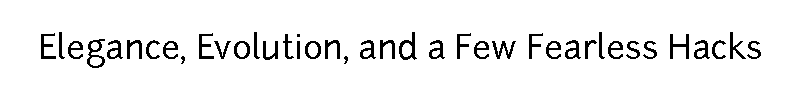
\includegraphics{../images/frontmatter/subtitle.eps}
\\[13.5cm]
\vspace{0.5cm}
\hspace{6.5cm}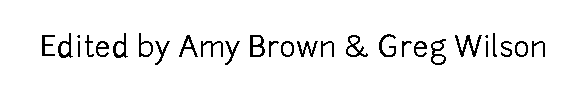
\includegraphics{../images/frontmatter/eds.eps}

\newpage
% copyright page 

\thispagestyle{empty}

\small
%% \noindent \textbf{The Architecture of Open Source Applications} \\
%% Edited by Amy Brown and Greg Wilson
\noindent \textbf{オープンソースアプリケーションのアーキテクチャ} \\
編集:Amy Brown and Greg Wilson \\
翻訳:TAKAGI Masahiro

\vspace{0.15cm}

\noindent
%% This work is licensed under the Creative Commons Attribution 3.0
%% Unported license (CC~BY~3.0).  You are free:
この日本語訳はCreative Commons表示3.0非移植ライセンス(CC~BY~3.0)のもとで公開します。あなたは以下の条件に従う限り、自由に

\begin{aosaitemize}
  %% \item to Share---to copy, distribute and transmit the work
  %% \item to Remix---to adapt the work
  \item 本作品を複製、頒布、展示、実演することができます。
  \item 二次的著作物を作成することができます。
  \item 本作品を営利目的で利用することができます。
\end{aosaitemize}

\noindent
%% under the following conditions:
あなたが従うべき条件は以下の通りです。

\begin{aosaitemize}
  %% \item Attribution---you must attribute the work in the manner
  %%   specified by the author or licensor (but not in any way that
  %%   suggests that they endorse you or your use of the work).
  \item 表示---あなたは原著作者のクレジットを表示しなければなりません。
\end{aosaitemize}

\noindent
%% with the understanding that:
以下のような理解に基づいています。

\begin{aosaitemize}

  %% \item Waiver---Any of the above conditions can be waived if you get
  %%   permission from the copyright holder.
  \item 放棄---この作品について著作権者等の権利者から別途許可を得た場合は、上記の許諾条件は適用されません。

  %% \item Public Domain---Where the work or any of its elements is in
  %%   the public domain under applicable law, that status is in no way
  %%   affected by the license.
  \item パブリック・ドメイン---作品やその要素が、適用される法律の下でパブリックドメインに属する場合、その状態がこのライセンスによって影響されることはありません。

  %% \item Other Rights---In no way are any of the following rights
  %%   affected by the license:
  \item そのほかの諸権利---ライセンスによって、以下の諸権利が影響を受けるということは全くありません。
    \begin{aosaitemize}

      %% \item Your fair dealing or fair use rights, or other applicable
      %%   copyright exceptions and limitations;
      \item あなたのフェア・ディーリングやフェア・ユースの権利、そのほか著作権の例外・制限規定

      \item The author's moral rights;

      \item Rights other persons may have either in the work itself or
        in how the work is used, such as publicity or privacy rights.

    \end{aosaitemize}

  %% \item Notice---For any reuse or distribution, you must make clear to
  %%   others the license terms of this work. The best way to do this is
  %%   with a link to \url{http://creativecommons.org/licenses/by/3.0/}.
  \item Notice---再利用や頒布にあたっては、この作品の使用許諾条件を他の人々に明らかにしなければなりません。一番よい方法は、\url{http://creativecommons.org/licenses/by/3.0/}へのリンクを示すことです。

\end{aosaitemize}

%% \noindent To view a copy of this license, visit
%% \url{http://creativecommons.org/licenses/by/3.0/} or send a letter to Creative
%% Commons, 444 Castro Street, Suite 900, Mountain View, California,
%% 94041, USA.\\
\noindent このライセンスのコピーを見るには、
\url{http://creativecommons.org/licenses/by/3.0/}を見るか、手紙をCreative
Commons, 444 Castro Street, Suite 900, Mountain View, California,
94041, USA.に送ってください。\\

\vspace{0.15cm}

\noindent
%% The full text of this book is available online at \url{http://www.aosabook.org/}.\\
%% All royalties from its sale will be donated to Amnesty International.\\
本書の全文は、\url{http://www.aosabook.org/}でオンラインで読めます。\\
(英語版の)印税はすべて、アムネスティ・インターナショナルに寄付されます。\\

\vfill

%% \noindent Product and company names mentioned herein may be the trademarks of
%% their respective owners.\\
\noindent 本書に記載されている製品名や会社名は、各社の登録商標あるいは商標である可能性があります。\\

\vspace{0.15cm}

%% \noindent While every precaution has been taken in the preparation of this
%% book, the editors and authors assume no responsibility for errors or omissions,
%% or for damages resulting from the use of the information contained herein.\\
\noindent 本書の製作にあたっては十分に注意を払いましたが、編集者や執筆者そして翻訳者は本書の内容についてなんらかの保証をするものではなく、その内容に基づくいかなる被害に関しても一切の責任を負いません。\\

\vspace{0.15cm}

%% \noindent The cover image is a photograph by Peter Dutton. The photograph is
%% licensed under the Creative Commons Attribution-NonCommercial-ShareAlike 2.0
%% Generic license. To view a copy of this license, visit
%% \url{http://creativecommons.org/licenses/by-nc-sa/2.0/} or send a letter to
%% CreativeCommons, 444 Castro Street, Suite 900, Mountain View, California,
%% 94041, USA. \\
\noindent 表紙の画像はPeter Duttonが撮影した写真です。この写真はCreative Commons表示 - 非営利 - 継承 2.0 一般でライセンスされています。このライセンスのコピーを見るには、
\url{http://creativecommons.org/licenses/by-nc-sa/2.0/}を見るか、手紙を
CreativeCommons, 444 Castro Street, Suite 900, Mountain View, California,
94041, USA.に送ってください。\\

\vspace{1cm}

\noindent Revision Date: \today \\

%% \noindent ISBN: 978-1-257-63801-7
\normalsize

\newpage
% Dedication page

\thispagestyle{empty}

\vspace*{5cm}
\begin{center}
%% \hspace{0cm}Dedicated to Brian Kernighan,\\
%% who has taught us all so much;\\
%% and to prisoners of conscience everywhere.
\hspace{0cm}我々に多くのことを教えてくれたBrian Kernighanに\\
そして世界中にいる良心の囚人たちに
\end{center}

\newpage

% Blank page here
\thispagestyle{empty}
\mbox{}    % need to have *something* in here or Latex "helpfully" removes page



\tableofcontents

%% \begin{aosachapter}{Introduction}{s:intro}{Amy Brown and Greg Wilson}
%% Based on EN-Revision r229
\begin{aosachapter}{導入}{s:intro}{Amy Brown \& Greg Wilson}

%% Carpentry is an exacting craft, and people can spend their entire
%% lives learning how to do it well.  But carpentry is not architecture:
%% if we step back from pitch boards and miter joints, buildings as a
%% whole must be designed, and doing that is as much an art as it is a
%% craft or science.
大工仕事は非常に奥の深いものであり、人はみな、上達するための方法を一生涯かけて学び続けることになる。しかし、大工仕事と建築様式は異なる。ピッチ板や留め継ぎの世界から一歩離れて見渡せば、建造物全体を見た設計が必要になる。そしてそれは、技術的・科学的であるのと同程度に芸術の要素もある。

%% Programming is also an exacting craft, and people can spend their entire lives
%% learning how to do it well.  But programming is not software architecture. 
%% Many programmers spend years thinking about
%% (or wrestling with) larger design issues: Should this application be
%% extensible?  If so, should that be done by providing a scripting
%% interface, through some sort of plugin mechanism, or in some other way
%% entirely?  What should be done by the client, what should be left to
%% the server, and is ``client-server'' even a useful way to think about
%% this application?  These are not programming questions, any more than
%% where to put the stairs is a question of carpentry.
プログラミングもまた奥の深い作業であり、人はみな、上達するための方法を一生涯かけて学び続けることになる。しかし、プログラミングとソフトウェアアーキテクチャは異なる。多くのプログラマは、何年もかけて大規模な設計の問題に取り組む。「このアプリケーションを拡張可能にすべきだろうか?」「仮にそうだとして、その手法はどうする?スクリプトで拡張できるようにするのかプラグイン的な仕組みを取り入れるのか、あるいはまったく異なる別の方法を考える?」「クライアント側でやるべき処理とサーバー側でやるべき処理の切り分けはどうする?そもそもこのアプリケーションを``クライアント・サーバー''型で考えるのは適切なのか?」といった問題だ。これらの問いは、プログラミングに関するものではない。「階段をどこに配置するか」という問いが大工仕事とは関係ないのと同じことだ。

%% Building architecture and software architecture have a lot in common,
%% but there is one crucial difference.  While architects study
%% thousands of buildings in their training and during their careers,
%% most software developers only ever get to know a handful of large
%% programs well.  And more often than not, those are programs they wrote
%% themselves.  They never get to see the great programs of history, or
%% read critiques of those programs' designs written by experienced
%% practitioners.  As a result, they repeat one another's mistakes rather
%% than building on one another's successes.
建築様式とソフトウェアアーキテクチャには共通点も多いが、決定的な違いがひとつある。建築家はその生涯を通じて何千ものビルについて研究を重ねるが、大半のソフトウェア開発者はほんの一握りの大規模ソフトウェアしか知ることがない。しかも、その数少ないソフトウェアは自分たちが書いたものであることが多い。ソフトウェア開発者は歴史上の偉大なプログラムを振り返ることもないし、そういったプログラムの設計に関する熟練者の批評を読むこともない。その結果、先人の成功例を参考にすることもできずに同じ過ちを繰り返す。

%% This book is our attempt to change that.  Each chapter describes the
%% architecture of an open source application: how it is structured, how
%% its parts interact, why it's built that way, and what lessons have
%% been learned that can be applied to other big design problems.  The
%% descriptions are written by the people who know the software
%% best, people with years or decades of experience designing and
%% re-designing complex applications.  The applications themselves range
%% in scale from simple drawing programs and web-based spreadsheets to
%% compiler toolkits and multi-million line visualization packages.  Some
%% are only a few years old, while others are approaching their thirtieth
%% anniversary.  What they have in common is that their creators have
%% thought long and hard about their design, and are willing to share
%% those thoughts with you.  We hope you enjoy what they have written.
そんな状況をどうにかしたいと思って本書を書いた。各章では、オープンソースアプリケーションのアーキテクチャについて解説している。どのような構造になっているのか、各パーツがどのように絡み合っているのか、なぜその方式を採用したのか、他の設計上の問題に適用できそうな教訓は何か、といった内容だ。執筆者はそのソフトウェアをもっともよく知る人たちで、何年あるいは何十年もの間、複雑なアプリケーションの設計を経験してきた。本書ではさまざまなアプリケーションを取り上げる。シンプルなドローツールやウェブベースの表計算ソフトもあれば、コンパイラツールキットや数百万行規模の視覚化パッケージもある。数年前に生まれたばかりのアプリケーションもあれば、30周年を迎えるアプリケーションもある。すべてのアプリケーションに共通しているのは、作者が長い時間をかけて真剣に設計を考えたこと。そしてその考えを皆で分かち合いたいと考えているということだ。きっと読者のみなさんにも楽しんでもらえるだろう。

%% \section*{Contributors}
\section*{執筆者}

%% \indent \indent \emph{Eric P\@. Allman (Sendmail)}: Eric Allman is the
%% original author of sendmail, syslog, and trek, and the co-founder
%% of Sendmail, Inc.  He has been writing open source software since
%% before it had a name, much less became a ``movement''.  He is a
%% member of the \emph{ACM Queue} Editorial Review Board and the Cal
%% Performances Board of Trustees.  His personal web site
%% is \url{http://www.neophilic.com/~eric}.
\indent \indent \emph{Eric P\@. Allman (Sendmail)}: Eric Allmanはsendmailやsyslogそしてtrekの原作者であり、Sendmail, Inc.の共同創業者でもある。彼がオープンソースソフトウェアを書き始めたころにはまだ``オープンソース''などという名前はついておらず、ましてや今のような``ブーム''にはなっていなかった。彼は\emph{ACM Queue} Editorial Review BoardおよびCal Performances Board of Trusteesのメンバーである。個人サイトは\url{http://www.neophilic.com/~eric}だ。

%% \pagebreak

%% \emph{Keith Bostic (Berkeley DB)}: Keith was a member of the University
%% of California Berkeley Computer Systems Research Group, where he was the
%% architect of the 2.10BSD release and a principal developer of 4.4BSD and
%% related releases.  He received the USENIX Lifetime Achievement Award (``The
%% Flame''), which recognizes singular contributions to the Unix community, as well
%% as a Distinguished Achievement Award from the University of California,
%% Berkeley, for making the 4BSD release open source.  Keith was the
%% architect and one of the original developers of Berkeley DB, the open source
%% embedded database system.  
\emph{Keith Bostic (Berkeley DB)}: Keithはカリフォルニア大学バークレー校のComputer Systems Research Groupのメンバーだった。そこで2.10BSDリリースのアーキテクトや4.4BSDおよび関連リリースの開発リーダーをつとめた。彼はUSENIX Lifetime Achievement Award (``The Flame'')を受賞した。これはUnixコミュニティへの並はずれた貢献を認められたものだ。また、カリフォルニア大学バークレー校からDistinguished Achievement Awardも受賞している。これは4BSDリリースをオープンソースにしたことに対するものだ。KeithはBerkeley DBのアーキテクトかつ開発者の一員だった。Berkeley DBは、オープンソースの組み込みデータベースシステムである。

%% \emph{Amy Brown (editorial)}: Amy has a bachelor's degree in Mathematics
%% from the University of Waterloo, and worked in the software industry for ten
%% years.  She now writes and edits books, sometimes about software. She also
%% sings and organizes other people's lives---professionally and recreationally.
\emph{Amy Brown (編集担当)}: Amyはウォータールー大学で数学の学士号を取得し、ソフトウェア業界で10年の勤務経験を持つ。現在は、書籍の執筆や編集に携わりつつ時にはソフトウェアも書く。彼女は歌手でもあり、他の人のライブを仕切ったりもする - プロもいれば趣味の人もいる。

%% \emph{C. Titus Brown (Continuous Integration)}: Titus has worked in
%% evolutionary modeling, physical meteorology, developmental biology, genomics,
%% and bioinformatics. He is now an Assistant Professor at Michigan State
%% University, where he has expanded his interests into several new areas,
%% including reproducibility and maintainability of scientific software. He is
%% also a member of the Python Software Foundation, and blogs at
%% \url{http://ivory.idyll.org}.
\emph{C. Titus Brown (Continuous Integration)}: Titusは、進化的モデリングや物理気象学、発生生物学、ゲノミクス、そしてバイオインフォマティクスを研究している。現在はミシガン州立大学の准教授であり、科学的ソフトウェアの再現性や保守性にまで興味の範囲を広げている。彼はPython Software Foundationのメンバーでもあり、ブログは\url{http://ivory.idyll.org}にある。

%% \emph{Roy Bryant (Snowflock)}: In 20 years as a software
%% architect and CTO, Roy designed systems including Electronics
%% Workbench (now National Instruments' Multisim) and the Linkwalker
%% Data Pipeline, which won Microsoft's worldwide Winning Customer
%% Award for High-Performance Computing in 2006. After selling his
%% latest startup, he returned to the University of Toronto to do
%% graduate studies in Computer Science with a research focus on
%% virtualization and cloud computing. Most recently, he published
%% his Kaleidoscope extensions to Snowflock at ACM's Eurosys
%% Conference in 2011.  His personal web site
%% is \url{http://www.roybryant.net/}.
\emph{Roy Bryant (Snowflock)}: ソフトウェアアーキテクトおよびCToとして20年の経験を持つRoyは、Electronics Workbench(現在のNational Instruments' Multisim)やLinkwalker Data Pipelineといったシステムを設計した。Linkwalker Data Pipelineは、Microsoft's worldwide Winning Customer Award for High-Performance Computingを2006年に受賞した。最後に在籍したスタートアップを売却した彼はトロント大学に戻り、大学院でコンピュータサイエンスを研究している。専門は、ビジュアライゼーションとクラウドコンピューティングだ。最近は、ACMのEurosys Conference in 2011でSnowflock用のKaleidoscope拡張について発表した。個人サイトは\url{http://www.roybryant.net/}である。

%% \emph{Russell Bryant (Asterisk)}: Russell is the Engineering
%% Manager for the Open Source Software team at Digium, Inc. He has
%% been a core member of the Asterisk development team since the Fall
%% of 2004. He has since contributed to almost all areas of Asterisk
%% development, from project management to core architectural design
%% and development.  He blogs at
%% \url{http://www.russellbryant.net}.
\emph{Russell Bryant (Asterisk)}: RussellはDigium, Inc.のオープンソースソフトウェアチームでエンジニアリングマネージャーを務めている。また、2004年の秋からAsterisk開発チームのコアメンバーとして活動している。これまでに、Asteriskの開発におけるほぼすべての分野に貢献をしてきた。プロジェクトの運営からアーキテクチャ設計、そして開発まで。彼のブログは\url{http://www.russellbryant.net}である。

%% \emph{Rosangela Canino-Koning (Continuous Integration)}:
%% After 13 years of slogging in the software industry trenches,
%% Rosangela returned to university to pursue a Ph.D.\ in Computer
%% Science and Evolutionary Biology at Michigan State University. In
%% her copious spare time, she likes to read, hike, travel, and hack
%% on open source bioinformatics software.  She blogs at
%% \url{http://www.voidptr.net}.
\emph{Rosangela Canino-Koning (Continuous Integration)}: ソフトウェア業界の最前線での13年間を経てRosangelaは大学に戻り、ミシガン州立大学でコンピュータサイエンスと進化生物学の博士号取得を目指している。空き時間には読書やハイキング、旅行などを楽しむほか、オープンソースのバイオインフォマティクスソフトウェアをハックすることもある。彼女のブログは\url{http://www.voidptr.net}である。

%% \emph{Francesco Cesarini (Riak)}: Francesco Cesarini has
%% used Erlang on a daily basis since 1995, having worked in various
%% turnkey projects at Ericsson, including the OTP R1 release. He is
%% the founder of Erlang Solutions and co-author of
%% O'Reilly's \emph{Erlang Programming}. He currently works as
%% Technical Director at Erlang Solutions, but still finds the time
%% to teach graduates and undergraduates alike at Oxford University in
%% the UK and the IT University of Gotheburg in Sweden.
\emph{Francesco Cesarini (Riak)}: Francesco CesariniがErlangを常用しはじめたのは1995年のことだった。その後もEricssonでさまざまなプロジェクトに参加し、OTP R1リリースにもかかわっている。彼はErlang Solutionsの創設者であり、O'Reillyの\emph{Erlang Programming}の共著者でもある。現在はErlang Solutionsのテクニカルディレクターとして働いているが、イギリスのオックスフォード大学やスウェーデンのヨーテボリ大学で学生や院生を教えることもある。

%% \emph{Robert Chansler (HDFS)}: Robert is a Senior Manager for Software
%% Development at Yahoo!  After graduate studies in distributed systems
%% at Carnegie-Mellon University, he worked on compilers (Tartan Labs),
%% printing and imaging systems (Adobe Systems), electronic commerce
%% (Adobe Systems, Impresse), and storage area network management
%% (SanNavigator, McDATA). Returning to distributed systems and HDFS, Rob
%% found many familiar problems, but all of the numbers had two or three
%% more zeros.
\emph{Robert Chansler (HDFS)}: RobertはYahoo!に在籍するソフトウェア開発のシニアマネージャーである。カーネギーメロン大学の大学院で分散システムを研究した彼はその後、コンパイラ(Tartan Labs)、印刷・画像処理システム(Adobe Systems)、電子商取引(Adobe Systems, Impresse)、SAN管理(SanNavigator, McDATA)などにかかわった。分散システムやHDFSの世界に戻ってきた彼は、解決すべき課題が以前とあまり変わっていないことに気付いた。しかし、登場する数値はどれもみな、ゼロが2つか3つ多くなっていた。

%% \emph{James Crook (Audacity)}: James is a contract software
%% developer based in Dublin, Ireland. Currently he is working on
%% tools for electronics design, though in a previous life he
%% developed bioinformatics software.  He has many audacious plans
%% for Audacity, and he hopes some, at least, will see the light of day.
\emph{James Crook (Audacity)}: Jamesはアイルランドのダブリンに住むソフトウェア開発者。現在は電子工学設計用のツールにかかわっているが、かつてはバイオインフォマティクスソフトウェアを開発していたこともある。彼はAudacityに関する多くの野望を抱えており、その中のいくつかだけでも日の目を見ることを望んでいる。

%% \pagebreak

%% \emph{Chris Davis (Graphite)}: Chris is a software
%% consultant and Google engineer who has been designing and building
%% scalable monitoring and automation tools for over 12 years. Chris
%% originally wrote Graphite in 2006 and has lead the open source
%% project ever since. When he's not writing code he enjoys cooking,
%% making music, and doing research. His research interests include
%% knowledge modeling, group theory, information theory, chaos
%% theory, and complex systems.
\emph{Chris Davis (Graphite)}: Chrisはソフトウェアコンサルタントであり、Googleのエンジニアとしてスケーラブルな監視・自動化ツールの設計と構築に12年以上携わっている。ChrisがGraphiteを書き始めたのは2006年で、それ以降ずっとこのプロジェクトを率いている。コードを書いていないときの彼は、料理や作曲そして研究などをしている。彼の研究分野は、知識モデリングや群論、情報理論、カオス理論、そして複雑系などだ。

%% \emph{Juliana Freire (VisTrails)}: Juliana is an Associate Professor
%% of Computer Science at the University of Utah. Before that, she was member
%% of technical staff at the Database Systems Research Department at Bell
%% Laboratories (Lucent Technologies) and an Assistant Professor at
%% OGI/OHSU\@. Her research interests include provenance, scientific data
%% management, information integration, and Web mining.  She is a
%% recipient of an NSF CAREER and an IBM Faculty award.  Her research has
%% been funded by the National Science Foundation, Department of Energy,
%% National Institutes of Health, IBM, Microsoft and Yahoo!
\emph{Juliana Freire (VisTrails)}: Julianaは、ユタ大学のコンピュータサイエンスの准教授である。それ以前には、ベル研究所(ルーセント・テクノロジーズ)のデータベースシステム研究部門に在籍したりオレゴン健康科学大学/オレゴン科学技術大学院大学に準教授として在籍したりしていた。彼女の研究分野は、起源や科学データ管理、情報統合、そしてウェブマイニングなどだ。彼女はNSF CAREERおよびIBM Faculty Awardを受賞している。また、彼女の研究に対して国立科学財団やエネルギー省、国立衛生研究所、そしてIBMやMicrosoft、Yahoo!が資金提供している。

%% \emph{Berk Geveci (VTK)}: Berk is the Director of Scientific
%% Computing at Kitware. He is responsible for leading the
%% development effort of ParaView, an award-winning visualization
%% application based on VTK\@. His research interests include large
%% scale parallel computing, computational dynamics, finite elements
%% and visualization algorithms.
\emph{Berk Geveci (VTK)}: Berkは、Kitwareで科学計算のリーダーを務めている。彼はParaViewの開発リーダーでもある。ParaViewは、VTK\@をベースとした視覚化アプリケーションである。彼の研究分野は、大規模なパラレルコンピューティングや計算力学、有限要素、そして視覚化アルゴリズムだ。

%% \emph{Andy Gross (Riak)}: Andy Gross is Principal Architect at Basho
%% Technologies, managing the design and development of Basho's Open
%% Source and Enterprise data storage systems. Andy started at Basho in
%% December of 2007 with 10 years of software and distributed systems
%% engineering experience.  Prior to Basho, Andy held senior distributed
%% systems engineering positions at Mochi Media, Apple, Inc., and Akamai
%% Technologies.
\emph{Andy Gross (Riak)}: Andy GrossはBasho Technologiesのアーキテクト長であり、Bashoのオープンソースおよびエンタープライズデータストレージシステムの設計と開発を仕切っている。AndyがBashoを立ち上げたのは2007年12月。10年におよぶソフトウェア開発や分散システムエンジニアリングの経験を経た後のことだった。Bashoの前にAndyは、分散システムエンジニアリングの上級技術者としてMochi MediaやApple, Inc.、Akamai Technologiesなどに勤めていた。

%% \emph{Bill Hoffman (CMake)}: Bill is CTO and co-Founder of
%% Kitware, Inc.  He is a key developer of the CMake project, and has
%% been working with large C++ systems for over 20 years.
\emph{Bill Hoffman (CMake)}: BillはKitware, Inc.のCTOを務める共同創業者である。彼はCMakeプロジェクトの主要な開発者であり、大規模なC++システムに20年以上携わってきた経験を持つ。

%% \emph{Cay Horstmann (Violet)}: Cay is a professor of
%% computer science at San Jose State University, but every so often
%% he takes a leave of absence to work in industry or teach in a
%% foreign country.  He is the author of many books on programming
%% languages and software design, and the original author of the
%% Violet and GridWorld open-source programs.
\emph{Cay Horstmann (Violet)}: Cayはサンノゼ州立大学でコンピュータサイエンスの教授を務めるが、しょっちゅう休暇をとっては業界で働いていたり外国で教えていたりする。プログラミング言語やソフトウェア設計に関する多くの著作があり、オープンソースのVioletやGridWorldの原作者でもある。

%% \emph{Emil Ivov (Jitsi)}: Emil is the founder and project
%% lead of the Jitsi project (previously SIP Communicator). He is
%% also involved with other initiatives like the ice4j.org and JAIN
%% SIP projects. Emil obtained his Ph.D.\ from the University of
%% Strasbourg in early 2008, and has been focusing primarily on Jitsi
%% related activities ever since.
\emph{Emil Ivov (Jitsi)}: EmilはJitsiプロジェクト(かつてはSIP Communicatorと呼ばれていた)の創設者であり、プロジェクトを率いている。彼は、ice4j.orgやJAIN SIPプロジェクトなど他の場所でも活躍している。Emilは2008年初めにストラスブール大学で博士号を取得した。それ以降は、Jitsi関連の活動に重点を置いている。

%% \emph{David Koop (VisTrails)}: David is a Ph.D.\ candidate in computer
%% science at the University of Utah (finishing in the summer of
%% 2011). His research interests include visualization, provenance, and
%% scientific data management. He is a lead developer of the VisTrails
%% system, and a senior software architect at VisTrails, Inc.
\emph{David Koop (VisTrails)}: Davidはユタ大学のコンピュータサイエンスの博士候補(2011年夏に修了予定)。彼の研究分野は、視覚化や起源そして科学データ管理だ。彼はVisTrailsシステムのリード開発者であり、VisTrails, Inc.の上級ソフトウェアアーキテクトである。

%% \emph{Hairong Kuang (HDFS)} is a long time contributor and committer
%% to the Hadoop project, which she has worked on passionately, currently
%% at Facebook and previously at Yahoo! Prior to working in industry, she was an
%% Assistant Professor at California State Polytechnic University,
%% Pomona. She received a Ph.D.\ in Computer Science from the University of
%% California at Irvine.  Her interests include cloud computing, mobile
%% agents, parallel computing, and distributed systems.
\emph{Hairong Kuang (HDFS)} は、貢献者およびコミッターとして長期にわたってHadoopプロジェクトに長年かかわってきた。かつてはYahoo!で、そして現在はFacebookで働いている。業界で働くようになる前は、彼女はカリフォルニア州立工科大学ポモナ校の准教授だった。カリフォルニア大学アーバイン校でコンピュータサイエンスの博士号を取得している。彼女の研究分野は、クラウドコンピューティングやモバイルエージェント、パラレルコンピューティング、そして分散システムである。

%% \emph{H.\ Andr\'{e}s Lagar-Cavilla (Snowflock)}:
%% Andr\'{e}s is a software systems researcher who does
%% experimental work on virtualization, operating systems, security,
%% cluster computing, and mobile computing. He has a B.A.Sc.\ from
%% Argentina, and an M.Sc.\ and Ph.D.\ in Computer Science from University
%% of Toronto, and can be found online
%% at \url{http://lagarcavilla.org}.
\emph{H.\ Andr\'{e}s Lagar-Cavilla (Snowflock)}: Andr\'{e}sはソフトウェアシステムの研究者で、視覚化やオペレーティングシステム、セキュリティ、クラスタコンピューティング、モバイルコンピューティングなどを対象としている。学士号はアルゼンチンで、そしてコンピュータサイエンスの修士号と博士号はトロント大学で取得した。オンラインでは\url{http://lagarcavilla.org}で活動している。

%% \emph{Chris Lattner (LLVM)}: Chris is a software developer
%% with a diverse range of interests and experiences, particularly in
%% the area of compiler tool chains, operating systems, graphics and
%% image rendering.  He is the designer and lead architect of the
%% Open Source LLVM Project.
%% See \url{http://nondot.org/~sabre/}
%% for more about Chris and his projects.
\emph{Chris Lattner (LLVM)}: Chrisはソフトウェア開発者で、幅広い分野の経験を持つ。コンパイラツール群やオペレーティングシステム、そしてグラフィックや画像レンダリングが得意分野だ。彼は、オープンソースのLLVMプロジェクトの設計者でありリードアーキテクトである。Chrisや彼のプロジェクトに関する詳細な情報は\url{http://nondot.org/~sabre/}で得られる。

%% \emph{Alan Laudicina (Thousand Parsec)}: Alan is an M.Sc.\ 
%% student in computer science at Wayne State University, where he
%% studies distributed computing. In his spare time he codes, learns
%% programming languages, and plays poker.  You can find more about
%% him at \url{http://alanp.ca/}.
\emph{Alan Laudicina (Thousand Parsec)}: Alanはウェイン州立大学の修士課程の学生で、分散コンピューティングを学んでいる。空き時間には、コードを書いたりプログラミング言語を学んだり、あるいはポーカーをプレイしたりする。詳細な情報は\url{http://alanp.ca/}で得られる。

%% \emph{Danielle Madeley (Telepathy)}: Danielle is an
%% Australian software engineer working on Telepathy and other magic
%% for Collabora Ltd. She has bachelor's degrees in electronic
%% engineering and computer science. She also has an extensive
%% collection of plush penguins.  She blogs
%% at \url{http://blogs.gnome.org/danni/}.
\emph{Danielle Madeley (Telepathy)}: Danielleはオーストラリアのソフトウェアエンジニアで、Collabora Ltd.でTelepathyその他の開発にかかわっている。彼女は電子工学とコンピュータサイエンスの学士号を持っており、Plush Penguinを収集している。ブログは\url{http://blogs.gnome.org/danni/}である。

%% \emph{Adam Marcus (NoSQL)}: Adam is a Ph.D.\ student focused on the
%% intersection of database systems and social computing at MIT's Computer Science
%% and Artificial Intelligence Lab.  His recent work ties traditional database
%% systems to social streams such as Twitter and human computation platforms such
%% as Mechanical Turk. He likes to build usable open source systems from his
%% research prototypes, and prefers tracking open source storage systems to long
%% walks on the beach. He blogs at \url{http://blog.marcua.net}.
\emph{Adam Marcus (NoSQL)}: Adamは博士課程の学生で、データベースシステムとソーシャルコンピューティングの共通部分をMITコンピュータ科学・人工知能研究所で研究している。最近の研究内容は、伝統的なデータベースシステムとTwitterのようなソーシャルストリーム・Mechanical Turkのようなヒューマンコンピューティング環境との関係だ。研究用のプロトタイプを便利なオープンソースシステムに仕上げるのが好き。オープンソースのストレージシステムを追いかけているほうがビーチを歩くよりも好き。ブログは\url{http://blog.marcua.net}である。

%% \emph{Kenneth Martin (CMake)}: Ken is currently Chairman
%% and CFO of Kitware, Inc., a research and development company based
%% in the US\@. He co-founded Kitware in 1998 and since then has helped
%% grow the company to its current position as a leading R\&D
%% provider with clients across many government and commercial
%% sectors.
\emph{Kenneth Martin (CMake)}: Kenは現在Kitware, Inc.の会長とCFOを務める。Kitware, Inc.は米国に基盤をおく研究開発会社である。彼はKitwareを1998年に立ち上げた共同創業者であり、会社を現在のポジションに引き上げるのに貢献した。今や同社は一流のR\&Dプロバイダであり、政府機関や商業関係などさまざまな分野にまたがるクライアントを抱えている。

%% \emph{Aaron Mavrinac (Thousand Parsec)}: Aaron is a
%% Ph.D.\ candidate in electrical and computer engineering at the
%% University of Windsor, researching camera networks, computer
%% vision, and robotics. When there is free time, he fills some of it
%% working on Thousand Parsec and other free software, coding in
%% Python and C, and doing too many other things to get good at any
%% of them.  His web site is \url{http://www.mavrinac.com}.
\emph{Aaron Mavrinac (Thousand Parsec)}: Aaronは電子工学とコンピュータ工学をウィンザー大学で学ぶ博士候補で、カメラネットワークやコンピュータビジョン、そしてロボット工学を研究している。空き時間には、Thousand Parsecやその他のフリーソフトウェアに関する活動をしたりPythonやCのコードを書いたりその他さまざまなことに手を出している。彼のウェブサイトは\url{http://www.mavrinac.com}である。

%% \emph{Kim Moir (Eclipse)}: Kim works at the IBM Rational
%% Software lab in Ottawa as the Release Engineering lead for the
%% Eclipse and Runtime Equinox projects and is a member of the
%% Eclipse Architecture Council.  Her interests lie in build
%% optimization, Equinox and building component based software.
%% Outside of work she can be found hitting the pavement with her
%% running mates, preparing for the next road race.  She blogs at
%% \url{http://relengofthenerds.blogspot.com/}.
\emph{Kim Moir (Eclipse)}: KimはオタワにあるIBM Rational Softwareの研究所でEclipseやEquinoxプロジェクトのリリースエンジニアリングを率いる。またEclipse Architecture Councilのメンバーでもある。彼女が興味を持っている分野は、ビルドの最適化やEquinoxそしてコンポーネントベースのソフトウェアを作ることだ。オフのときにはランニング仲間と道路を走り、次のロードレースに備えている。彼女のブログは\url{http://relengofthenerds.blogspot.com/}である。

%% \emph{Dirkjan Ochtman (Mercurial)}: Dirkjan graduated as a
%% Master in CS in 2010, and has been working at a financial startup
%% for 3 years. When not procrastinating in his free time, he hacks
%% on Mercurial, Python, Gentoo Linux and a Python CouchDB
%% library. He lives in the beautiful city of Amsterdam.  His
%% personal web site is \url{http://dirkjan.ochtman.nl/}.
\emph{Dirkjan Ochtman (Mercurial)}: Dirkjanは2010年にコンピュータサイエンスの修士課程を修了した。金融関係のスタートアップ企業での勤務経験は3年になる。自由な時間ができると、MercurialやPython、Gentoo LinuxそしてPythonのCouchDBライブラリをハックする。彼はアムステルダムの美しい都市に住んでいる。個人サイトは\url{http://dirkjan.ochtman.nl/}である。

%% \emph{Sanjay Radia (HDFS)}: Sanjay is the architect of the Hadoop
%% project at Yahoo!, and a Hadoop committer and Project Management
%% Committee member at the Apache Software Foundation. Previously he held
%% senior engineering positions at Cassatt, Sun Microsystems and INRIA
%% where he developed software for distributed systems and grid/utility
%% computing infrastructures. Sanjay has a Ph.D.\ in Computer Science from
%% University of Waterloo, Canada.
\emph{Sanjay Radia (HDFS)}: SanjayはYahoo!でHadoopプロジェクトのアーキテクトを務める。Hadoopのコミッターであり、Apache Software FoundationのProject Management Committeeのメンバーでもある。かつてはCassattやSun MicrosystemsそしてINRIAに勤務していた経験もあり、分散システムやグリッドコンピューティング基盤の開発に携わっていた。Sanjayは、カナダのウォータールー大学でコンピュータサイエンスの博士号を取得している。

%% \emph{Chet Ramey (Bash)}: Chet has been involved with bash
%% for more than twenty years, the past seventeen as primary
%% developer.  He is a longtime employee of Case Western Reserve
%% University in Cleveland, Ohio, from which he received his B.Sc.\  and
%% M.Sc.\ degrees.  He lives near Cleveland with his family and pets,
%% and can be found online at \url{http://tiswww.cwru.edu/~chet}.
\emph{Chet Ramey (Bash)}: Chetは20年以上bashにかかわっており、過去17年はメイン開発者だった。オハイオ州クリーブランドにあるケース・ウェスタン・リザーブ大学の永年勤続者である彼は、学士号と修士号もそこで取得した。クリーブランド近郊に家族やペットとともに住み、オンラインでは\url{http://tiswww.cwru.edu/~chet}にいる。

%% \emph{Emanuele Santos (VisTrails)}: Emanuele is a research scientist
%% at the University of Utah. Her research interests include scientific
%% data management, visualization, and provenance. She received her
%% Ph.D.\ in Computing from the University of Utah in 2010. She is also a
%% lead developer of the VisTrails system.
\emph{Emanuele Santos (VisTrails)}: Emanueleはユタ大学で研究をする科学者で、研究分野は科学データ管理や視覚化、起源である。彼女は2010年に、ユタ大学でコンピューティングの博士号を取得している。彼女はVisTrailsシステムのリード開発者でもある。

%% \emph{Carlos Scheidegger (VisTrails)}: Carlos has a Ph.D.\ in
%% Computing from the University of Utah, and is now a researcher at
%% AT\&T Labs--Research. Carlos has won best paper awards at IEEE
%% Visualization in 2007, and Shape Modeling International in 2008. His
%% research interests include data visualization and analysis, geometry
%% processing and computer graphics.
\emph{Carlos Scheidegger (VisTrails)}: Carlosはユタ大学でコンピューティングの博士号を取得し、今はAT\&T Labsの研究部門で研究者として働いている。2007年のIEEE Visualizationと2008年のShape Modeling Internationalでは最優秀論文に選ばれた。彼の研究分野は、データの視覚化と解析やジオメトリ処理、そしてコンピュータグラフィックスだ。

%% \emph{Will Schroeder (VTK)}: Will is President and
%% co-Founder of Kitware, Inc. He is a computational scientist by
%% training and has been one of the key developers of VTK\@. He enjoys
%% writing beautiful code, especially when it involves computational
%% geometry or graphics.
\emph{Will Schroeder (VTK)}: WillはKitware, Inc.の社長で共同創業者でもある。コンピュータサイエンスの教育を受けており、VTK\@の主要な開発者のひとりだ。彼は美しいコードを書くことを好む。特に計算幾何学やグラフィックに関するコードでは。

%% \emph{Margo Seltzer (Berkeley DB)}: Margo is the Herchel
%% Smith Professor of Computer Science at Harvard's School of
%% Engineering and Applied Sciences and an Architect at Oracle
%% Corporation.  She was one of the principal designers of Berkeley
%% DB and a co-founder of Sleepycat Software.  Her research interests
%% are in filesystems, database systems, transactional systems, and
%% medical data mining.  Her professional life is online at
%% \url{http://www.eecs.harvard.edu/~margo}, and she blogs at
%% \url{http://mis-misinformation.blogspot.com/}.
\emph{Margo Seltzer (Berkeley DB)}: Margoはハーバード工学・応用科学大学院でコンピュータサイエンスの教授を務め、Oracle Corporationでアーキテクトとしても働いている。彼女はBerkeley DBの設計者のひとりであり、Sleepycat Softwareの共同創業者でもある。彼女の研究分野は、ファイルシステムやデータベースシステム、トランザクションシステム、そして医療データマイニングである。研究者としての顔は\url{http://www.eecs.harvard.edu/~margo}で見られ、ブログは\url{http://mis-misinformation.blogspot.com/}にある。

%% \emph{Justin Sheehy (Riak)}: Justin is the CTO of Basho
%% Technologies, the company behind the creation of Webmachine and
%% Riak. Most recently before Basho, he was a principal scientist at
%% the MITRE Corporation and a senior architect for systems
%% infrastructure at Akamai. At both of those companies he focused on
%% multiple aspects of robust distributed systems, including
%% scheduling algorithms, language-based formal models, and
%% resilience.
\emph{Justin Sheehy (Riak)}: JustinはBasho TechnologiesのCTO。同社はWebmachineやRiakの制作にかかわっている。Bashoの前職は、MITRE Corporationの科学者そしてAkamaiのシステム基盤担当シニアアーキテクトだった。両社で彼が力を注いでいたのは堅牢な分散システムに関するさまざまな内容だった。スケジューリングのアルゴリズムや言語ベースの形式モデル、そして弾性などが含まれる。

%% \emph{Richard Shimooka (Battle for Wesnoth)}: Richard is a Research
%% Associate at Queen's University's Defence Management Studies Program in
%% Kingston, Ontario. He is also a Deputy Administrator and Secretary for the
%% Battle for Wesnoth. Richard has written several works examining the
%% organizational cultures of social groups, ranging from governments to open
%% source projects.
\emph{Richard Shimooka (Battle for Wesnoth)}: Richardは、オンタリオ州キングストンにあるクイーンズ大学のDefence Management Studies Programで研究員を務めている。彼はまた、Battle for Wesnothの管理者代理かつ長官でもある。Richardの著作には、ソーシャルグループ(政府からオープンソースプロジェクトまでの幅広いもの)の組織文化に関して調査したものがいくつかある。

%% \emph{Konstantin V. Shvachko (HDFS)}, a veteran HDFS developer, is a
%% principal Hadoop architect at eBay. Konstantin specializes in
%% efficient data structures and algorithms for large-scale distributed
%% storage systems. He discovered a new type of balanced trees, S-trees,
%% for optimal indexing of unstructured data, and was a primary developer
%% of an S-tree-based Linux filesystem, treeFS, a prototype of
%% reiserFS. Konstantin holds a Ph.D.\ in computer science from Moscow
%% State University, Russia. He is also a member of the Project
%% Management Committee for Apache Hadoop.
\emph{Konstantin V. Shvachko (HDFS)} はベテランのHDFS開発者で、eBayのHadoopアーキテクトのリーダーである。Konstantinの専門分野は、大規模な分散ストレージシステムのための効率的なデータ構造やアルゴリズムである。彼は平衡木の新しい方式であるS-treeを考案した。これは構造化されていないデータの索引付けに最適化されたものだ。また彼は、S-treeベースのLinuxファイルシステムであるtreeFSの初期の開発者だった。treeFSは、後のreiserFSの原型となった。Konstantinは、ロシアのモスクワ大学でコンピュータサイエンスの博士号を取得している。また、Apache HadoopのProject Management Committeeのメンバーでもある。

%% \emph{Claudio Silva (VisTrails)}: Claudio is a full professor of
%% computer science at the University of Utah. His research interests are
%% in visualization, geometric computing, computer graphics, and
%% scientific data management. He received his Ph.D.\ in computer science
%% from the State University of New York at Stony Brook in 1996. Later in
%% 2011, he will be joining the Polytechnic Institute of New York
%% University as a full professor of computer science and engineering.
\emph{Claudio Silva (VisTrails)}: Claudioは、ユタ大学のコンピュータサイエンスの正教授である。彼の研究分野は、視覚化や幾何学的コンピューティング、コンピュータグラフィックス、そして科学データ管理などだ。彼は1996年に、ニューヨーク州立大学ストーニブルック校でコンピュータサイエンスの博士号を取得した。2011年後半には、ニューヨーク大学ポリテクニック研究室にコンピュータサイエンスおよびエンジニアリングの正教授として合流する予定だ。

%% \emph{Suresh Srinivas (HDFS)}: Suresh works on HDFS as a software
%% architect at Yahoo! He is a Hadoop committer and PMC member at Apache
%% Software Foundation. Prior to Yahoo!, he worked at Sylantro Systems,
%% developing scalable infrastructure for hosted communication
%% services. Suresh has a bachelor's degree in Electronics and
%% Communication from National Institute of Technology Karnataka, India.
\emph{Suresh Srinivas (HDFS)}: Sureshは、Yahoo!のソフトウェアアーキテクトとしてHDFSにかかわっている。彼はHadoopのコミッターであり、Apache Software FoundationのPMCのメンバーでもある。Yahoo!の前にはSylantro Systemsで働いており、コミュニケーションサービスのホスティングのためのスケーラブルな基盤を開発していた。Sureshは、インドのカルナタカにあるナショナル工科大学でエレクトロニクスと通信の学位を取得した。

%% \emph{Simon Stewart (Selenium)}: Simon lives in London and
%% works as a Software Engineer in Test at Google. He is a core
%% contributor to the Selenium project, was the creator of WebDriver
%% and is enthusiastic about open source. Simon enjoys beer and
%% writing better software, sometimes at the same time.  His personal
%% home page is \url{http://www.pubbitch.org/}.
\emph{Simon Stewart (Selenium)}: Simonはロンドン在住で、Googleのソフトウェアテストエンジニアとして働いている。彼はSeleniumプロジェクトの主要な貢献者である。WebDriverの作者でもある彼は、オープンソースにほれ込んでいる。Simonが好きなのはビールを楽しむこととソフトウェアを書くことで、ときにはそれらを同時にすることもある。個人ホームページは\url{http://www.pubbitch.org/}である。

%% \emph{Audrey Tang (SocialCalc)}: Audrey is a self-educated programmer
%% and translator based in Taiwan.  She curently works at Socialtext,
%% where her job title is ``Untitled Page'', as well as at Apple as
%% contractor for localization and release engineering.  She previously
%% designed and led the Pugs project, the first working Perl 6
%% implementation; she has also served in language design committees for
%% Haskell, Perl 5, and Perl 6, and has made numerous contributions to
%% CPAN and Hackage.  She blogs at \url{http://pugs.blogs.com/audreyt/}.
\emph{Audrey Tang (SocialCalc)}: Audreyは、台湾在住のプログラマーであり翻訳家でもある。現在の勤務先はSocialtextで、彼女のそこでの役職は``Untitled Page''だ。また、Appleのローカライズやリリースエンジニアリングも請け負っている。彼女はかつてPugsプロジェクトを率いていた。これは実際に動作するPerl 6の初めての実装だった。また、CPANやHackageにも多大な貢献をしている。彼女のブログは\url{http://pugs.blogs.com/audreyt/}である。

%% \pagebreak

%% \emph{Huy T.\ Vo (VisTrails)}: Huy is receiving his Ph.D.\ from the
%% University of Utah in May 2011. His research interests include
%% visualization, dataflow architecture and scientific data
%% management. He is a senior developer at VisTrails, Inc. He also holds
%% a Research Assistant Professor appointment with the Polytechnic
%% Institute of New York University.
\emph{Huy T.\ Vo (VisTrails)}: Huyは、2011年5月にユタ大学で博士号を取得した。彼の研究分野は、視覚化やデータフローアーキテクチャ、そして科学データ管理などである。VisTrails, Inc.で上級開発者として働く。彼はまた、ニューヨーク大学ポリテクニック研究室で博士研究員となることも決まっている。

%% \emph{David White (Battle for Wesnoth)}: David is the founder and lead
%% developer of Battle for Wesnoth. David has been involved with several Open
%% Source video game projects, including Frogatto which he also co-founded. David
%% is a performance engineer at Sabre Holdings, a leader in travel technology. 
\emph{David White (Battle for Wesnoth)}: Davidは、Battle for Wesnothの創設者でありリード開発者である。Davidはこれまでにもいくつかのオープンソースビデオゲームプロジェクトにかかわってきた。共同で立ち上げたFrogattoもそのひとつだ。彼はSabre Holdingsのパフォーマンスエンジニアであり、旅行技術のリーダーでもある。

%% \emph{Greg Wilson (editorial)}: Greg has worked over the
%% past 25 years in high-performance scientific computing, data
%% visualization, and computer security, and is the author or editor
%% of several computing books (including the 2008 Jolt Award
%% winner \emph{Beautiful Code}) and two books for children.
%% Greg received a Ph.D.\ in Computer Science from the University of
%% Edinburgh in 1993.
\emph{Greg Wilson (編集担当)}: Gregは過去25年にわたって高性能科学計算やデータの視覚化、コンピュータセキュリティなどにかかわってきた。数冊のコンピュータ関連書籍(2008年のJolt Awardを受賞した\emph{Beautiful Code}など)に著者あるいは編集者としてかかわっており、こども向けの本も二冊出版している。Gregは1993年にエジンバラ大学でコンピュータサイエンスの博士号を取得した。

%% \emph{Tarek Ziad\'{e} (Python Packaging)}: Tarek lives in Burgundy, France.
%% He's a Senior Software Engineer at Mozilla, building servers in Python. In his
%% spare time, he leads the packaging effort in Python.
\emph{Tarek Ziad\'{e} (Python Packaging)}: Tarekはフランスのブルゴーニュに住む。Mozillaの上級ソフトウェアエンジニアであり、サーバーをPythonで構築している。空き時間には、Pythonのパッケージングを率いている。

%% \section*{Acknowledgments}
\section*{謝辞}

%% We would like to thank our reviewers:\\
レビュアーのみなさんに感謝する。\\

\begin{tabular}{lll}
Eric Aderhold		& Muhammad Ali			& Lillian Angel		\\
Robert Beghian		& Taavi Burns			& Luis Pedro Coelho	\\
David Cooper		& Mauricio de Simone		& Jonathan Deber	\\
Patrick Dubroy		& Igor Foox			& Alecia Fowler		\\
Marcus Hanwell		& Johan Harjono			& Vivek Lakshmanan	\\
Greg Lapouchnian	& Laurie MacDougall Sookraj	& Josh McCarthy		\\
Jason Montojo		& Colin Morris			& Christian Muise	\\
Victor Ng		& Nikita Pchelin		& Andrew Petersen	\\
Andrey Petrov		& Tom Plaskon			& Pascal Rapicault	\\
Todd Ritchie		& Samar Sabie			& Misa Sakamoto		\\
David Scannell		& Clara Severino		& Tim Smith		\\
Kyle Spaans		& Sana Tapal			& Tony Targonski	\\
Miles Thibault		& David Wright			& Tina Yee
\end{tabular}

~\\

%% \noindent We would also like to thank Jackie Carter, who helped with the early stages of editing.
\noindent また、編集の初期段階での助けとなったJackie Carterにも感謝する。

%% \section*{Contributing}
\section*{貢献}

%% Dozens of volunteers worked hard to create this book, but there is
%% still lots to do.  You can help by reporting errors, by helping to
%% translate the content into other languages, or by describing the
%% architecture of other open source projects.  Please contact us at
%% \code{aosa@aosabook.org} if you would like to get involved.
何十人ものボランティアのおかげで本書を作ることができたが、まだやり残したことは多い。間違いの指摘、他の言語への翻訳、他のオープンソースプロジェクトのアーキテクチャに関する記述の追加などを歓迎する。協力してくれる場合は\code{aosa@aosabook.org}まで連絡してほしい。

\end{aosachapter}


\mainmatter
\begin{aosachapter}{Asterisk}{s:asterisk}{Russell Bryant}
%% Based on EN-Revision r229

%% Asterisk\footnote{\url{http://www.asterisk.org/}} is an open source telephony
%% applications platform distributed under the GPLv2. In short, it is a
%% server application for making, receiving, and performing custom
%% processing of phone calls.
Asterisk\footnote{\url{http://www.asterisk.org/}}はGPLv2で配布されているオープンソースによる電話通信のプラットフォームである。
簡単に言うと、電話を掛けたり、受けたり、カスタム処理を実行したりするためのサーバアプリケーションである。

%% The project was started by Mark Spencer in 1999. Mark had a company
%% called Linux Support Services and he needed a phone system to help
%% operate his business. He did not have a lot of money to spend on
%% buying one, so he just made his own. As the popularity of Asterisk
%% grew, Linux Support Services shifted focus to Asterisk and changed
%% its name to Digium, Inc.
このプロジェクトは 1999年にMark Spencerによって始められた。Markは自らが興した Linux Support Services社において、電話システムが必要だったのだが、購入するだけの費用が無かったために自作した。Asteriskの人気が上がると、Asteriskに資源を集中するため社名をDigium, Incに改めた。

%% The name Asterisk comes from the Unix wildcard character,
%% \code{*}. The goal for the Asterisk project is to do everything
%% telephony. Through pursuing this goal, Asterisk now supports a long
%% list of technologies for making and receiving phone calls. This
%% includes many VoIP (Voice over IP) protocols, as well as both analog
%% and digital connectivity to the traditional telephone network, or the
%% PSTN (Public Switched Telephone Network). This ability to get many
%% different types of phone calls into and out of the system is one of
%% Asterisk's main strengths.
Asteriskの名前の由来は、UNIXにおけるワイルドカード文字\code{*}にある。Asteriskプロジェクトの目標はすべての電話テクノロジを実装する事である。この目標に向けて、Asteriskは、電話を掛けたり、受けたりするための多くのテクノロジをサポートしている。これらのテクノロジには、従来のアナログおよびデジタルの電話ネットワークであるPSTN(Public Switched Telephone Network)はもちろん、多くのVoIP(Voice over IP)プロトコルも含まれる。このような異なる種類の電話テクノロジを実装していること、異なる電話テクノロジ同士を接続できる事がAsteriskの主な強みである。

%% Once phone calls are made to and from an Asterisk system, there are
%% many additional features that can be used to customize the processing
%% of the phone call. Some features are larger pre-built common
%% applications, such as voicemail. There are other smaller features that
%% can be combined together to create custom voice applications, such as
%% playing back a sound file, reading digits, or speech recognition.
Asteriskシステムに電話が掛かってきたり、Asteriskから電話を掛けたりするとき、通話処理をカスタマイズするのに使える多くの追加機能がある。ボイスメールのような完成されたアプリケーションもある一方、音声ファイルを流したり、数字を読んだり、音声認識といった、組み合せて使うことでカスタムの音声アプリケーションを構築するのに使えるようなより小規模の機能群もある。

%% \begin{aosasect1}{Critical Architectural Concepts}
\begin{aosasect1}{重要なアーキテクチャ・コンセプト}

%% This section discusses some architectural concepts that are critical
%% to all parts of Asterisk. These ideas are at the foundation of
%% the Asterisk architecture.
このセクションでは、Asterisk全体に影響するアーキテクチャのコンセプトについて述べる。
ここで述べる考え方は、Asteriskアーキテクチャの根幹を構成する。

%% \begin{aosasect2}{Channels}
\begin{aosasect2}{チャネル}

%% A channel in Asterisk represents a connection between the Asterisk
%% system and some telephony endpoint
%% (\aosafigref{fig.asterisk.simpleCall}). The most common example is
%% when a phone makes a call into an Asterisk system. This connection is
%% represented by a single channel. In the Asterisk code, a channel
%% exists as an instance of the \code{ast\_channel} data structure.  This
%% call scenario could be a caller interacting with voicemail, for
%% example.
Asteriskにおけるチャネルは、Asteriskシステムと電話端末の接続をあらわす(\aosafigref{fig.asterisk.simpleCall})。最も単純な例は、電話機がAsteriskシステムを呼び出す時である。この場合の接続は、一つのチャネルであらわされる。Asteriskのコードでは、チャネルは\code{ast\_channel} 構造体のインスタンスとして存在する。この呼び出しシナリオは、発信者がボイスメールを使うときの例である。

%% \aosafigure[225pt]{../images/asterisk/singleChannel.eps}{A Single Call Leg, Represented by a Single Channel}{fig.asterisk.simpleCall}
\aosafigure[225pt]{../images/asterisk/singleChannel.eps}{片方向通話, 単一チャネル}{fig.asterisk.simpleCall}

\end{aosasect2}

%% \begin{aosasect2}{Channel Bridging}
\begin{aosasect2}{チャネル・ブリッジ}

%% Perhaps a more familiar call scenario would be a connection between
%% two phones, where a person using phone A has called a person on phone
%% B\@. In this call scenario, there are two telephony endpoints connected
%% to the Asterisk system, so two channels exist for this call
%% (\aosafigref{fig.asterisk.twoChannels}).
おそらく、より馴染のある通話シナリオは電話機同士の接続であろう。このシナリオでは、電話機Aを使っている人が電話機B\@を呼び出す。すなわち2台の電話端末がAsteriskシステムに接続しているため、二つのチャネルが存在する(\aosafigref{fig.asterisk.twoChannels})。

\aosafigure[400pt]{../images/asterisk/twoChannels.eps}{2つのチャネルによって表される双方向通話}{fig.asterisk.twoChannels}

%% When Asterisk channels are connected like this, it is referred to as a
%% channel bridge. Channel bridging is the act of connecting channels
%% together for the purpose of passing media between them. The media
%% stream is most commonly an audio stream. However, there may also be a
%% video or a text stream in the call. Even in the case where there is
%% more than one media stream (such as both audio and video), it is still
%% handled by a single channel for each end of the call in Asterisk. In
%% \aosafigref{fig.asterisk.twoChannels}, where there are two channels
%% for phones A and B, the bridge is responsible for passing the media
%% coming from phone A to phone B, and similarly, for passing the media
%% coming from phone B to phone A\@. All media streams are negotiated
%% through Asterisk. Anything that Asterisk does not understand
%% and have full control over is not allowed. This means that Asterisk 
%% can do recording,
%% audio manipulation, and translation between different technologies.
このようにAsteriskチャネルが接続される事をチャネル・ブリッジと呼ぶ。チャネル・ブリッジは、チャネル同士をつなげて、メディアを流す事を目的としている。流れるメディアは音声が主になるが、ビデオやテキストも可能であるし、ひとつ以上のメディア(音声とビデオなど)のこともある。このような場合も、Asteriskでは、一つのチャネルとして扱われる。\aosafigref{fig.asterisk.twoChannels}では、2つのチャネルがそれぞれ、電話A、Bに接続されている。このブリッジは、電話機Aから電話機Bへのメディア・ストリームおよび電話機Bから電話機A\@へのメディア・ストリームを通すことに責任を持つ。すべてのメディア・ストリームは、Asteriskと交渉されるため、Asteriskが理解できない、またはフルにコントロールできないメディア・ストリームは許可されない。これは、Asteriskにおいて録音や音声処理、異なるテクノロジ間の変換が可能であることを意味する。

%% When two channels are bridged together, there are two methods that may
%% be used to accomplish this: generic bridging and native bridging.
%% A generic bridge is one that works regardless of what
%% channel technologies are in use. It passes all audio and signalling
%% through the Asterisk abstract channel interfaces. While this is the
%% most flexible bridging method, it is also the least efficient due to
%% the levels of abstraction necessary to accomplish the task.
%% \aosafigref{fig.asterisk.twoChannels} illustrates a generic bridge.
2つのチャネルをブリッジにより接続する形式は2通りある。ジェネリック・ブリッジとネイティブ・ブリッジである。
ジェネリック・ブリッジは、チャネル・テクノロジに何が使われていようが動作する。すべての音声とシグナリングは、Asterisk抽象チャネル・インタフェースを通してやりとりされる。これは、もっとも柔軟性の高い接続であるが、実現するために高いレベルの抽象化が必要であり、効率性を犠牲にしている。\aosafigref{fig.asterisk.twoChannels}は、ジェネリック・ブリッジを表現している。

%% A native bridge is a technology specific method of connecting channels
%% together. If two channels are connected to Asterisk using the same
%% media transport technology, there may be a way to connect them that is
%% more efficient than going through the abstraction layers in Asterisk
%% that exist for connecting different technologies together. For
%% example, if specialized hardware is being used for connecting to the
%% telephone network, it may be possible to bridge the channels on the
%% hardware so that the media does not have to flow up through the
%% application at all. In the case of some VoIP protocols, it is possible
%% to have endpoints send their media streams to each other directly,
%% such that only the call signalling information continues to flow
%% through the server.
ネイティブ・ブリッジは、テクノロジ固有のチャネル同士を接続するときに使われる手法である。2つのチャネルが、同じメディア・トランスポート・テクノロジを使ってAsteriskに接続されるときには、異なるテクノロジ同士を接続する時に使用するAsterisk抽象レイヤを通しての接続よりも、より効果的な接続方法がある。例えば、電話ネットワークに接続するのに特別のハードウェアが使われるときは、アプリケーションを全く通らずにチャネル同士をハードウェア上でブリッジする事が可能である。いくつかのVoIPプロトコルの場合には、呼制御信号の情報はサーバを通して流れるが、メディア・ストリームはエンドポイント間で相互に直接送受信させることも可能である。

%% The decision between generic bridging and native bridging is done by
%% comparing the two channels when it is time to bridge them. If both
%% channels indicate that they support the same native bridging method,
%% then that will be used. Otherwise, the generic bridging method will be
%% used. To determine whether or not two channels support the same native
%% bridging method, a simple C function pointer comparison is used. It's
%% certainly not the most elegant method, but we have not yet hit any
%% cases where this was not sufficient for our needs. Providing a native
%% bridge function for a channel is discussed in more detail in
%% \aosasecref{sec.asterisk.drivers}.
%% \aosafigref{fig.asterisk.nativeBridge} illustrates an example of a
%% native bridge.
ジェネリック・ブリッジかネイティブ・ブリッジかの選択は、ブリッジが必要になったときに、2つのチャネルの比較で決定される。二つのチャネルが同じネイティブ・ブリッジ技術をサポートする事がわかると、ネイティブ・ブリッジが使われる。その他の場合は、ジェネリック・ブリッジが使われる。2つのチャネルが同じネイティブ・ブリッジをサポートするかどうかの決定は、単純にC言語の関数ポインタの比較で行われる。これは、もっともエレガントな手法というわけではないが、この方法が我々のニーズを満たさなかったことは今のところない。ネイティブ・ブリッジ機能については、\aosasecref{sec.asterisk.drivers}で詳しく説明する。
\aosafigref{fig.asterisk.nativeBridge}は、ネイティブ・ブリッジの例を表現している。

%% \aosafigure{../images/asterisk/nativeBridge.eps}{Example of a Native Bridge}{fig.asterisk.nativeBridge}
\aosafigure{../images/asterisk/nativeBridge.eps}{ネイティブ・ブリッジの例}{fig.asterisk.nativeBridge}

\end{aosasect2}

%% \begin{aosasect2}{Frames}
\begin{aosasect2}{フレーム}

%% Communication within the Asterisk code during a call is done by using
%% frames, which are instances of the \code{ast\_frame} data
%% structure. Frames can either be media frames or signalling frames.
%% During a basic phone call, a stream of media frames containing audio
%% would be passing through the system. Signalling frames are used to send
%% messages about call signalling events, such as a digit being pressed, a
%% call being put on hold, or a call being hung up.
通話中のコミュニケーションは、Asteriskのコードではフレームで表現されている。これは、\code{ast\_frame}構造体のインスタンスである。フレームはメディア・フレームにもシグナリング・フレームにも使われる。音声メディア・フレームのストリームは基本的にシステムを通過する。シグナリング・フレームは、押された番号や保留中、呼切断などの呼制御イベントを送信するのに使われる。

%% The list of available frame types is statically defined. Frames are
%% marked with a numerically encoded type and subtype.  A full list can
%% be found in the source code in \code{include/asterisk/frame.h}; some
%% examples are:
利用可能なフレーム・タイプのリストは静的に定義される。フレーム・タイプは、タイプおよびサブタイプで記されて、数値の形式で保存される。フレーム・タイプの全リストはソースコードの \code{include/asterisk/frame.h}にある。代表的な例を以下に示す。

\begin{aosaitemize}

  %% \item \code{VOICE}: These frames carry a portion of an audio stream.
  \item \code{VOICE}: オーディオ・ストリーム・フレーム

  %% \item \code{VIDEO}: These frames carry a portion of a video stream.
  \item \code{VIDEO}: ビデオ・ストリーム・フレーム

  %% \item \code{MODEM}: The encoding used for the data in this frame,
  %% such as T.38 for sending a FAX over IP\@.  The primary usage of this
  %% frame type is for handling a FAX\@. It is important that frames of
  %% data be left completely undisturbed so that the signal can be
  %% successfully decoded at the other end. This is different than
  %% AUDIO frames, because in that case, it is acceptable to transcode
  %% into other audio codecs to save bandwidth at the cost of audio
  %% quality.
  \item \code{MODEM}: IP上でFAXを送信するためのT.38のようなデータに対する符号化を表わす\@。このフレーム・タイプの主な使用対象はFAXの処理である。この信号が相手側で正しく復号できるように、フレームのデータが絶対に変更されないことが重要である。これは、AUDIOフレームが帯域幅を稼ぐために音声品質を犠牲にしてコーデックを変換することが許されるという点で異なる。

  %% \item \code{CONTROL}: The call signalling message that this frame
  %% indicates.  These frames are used to indicate call signalling
  %% events. These events include a phone being answered, hung up, put
  %% on hold, etc.
  \item \code{CONTROL}: 呼制御メッセージを表わす。このフレームは、呼制御イベントを示すのに使われる。これらのイベントには、応答や切断、保留などがある。

  %% \item \code{DTMF\_BEGIN}: Which digit just started.  This frame is
  %%   sent when a caller presses a DTMF key\footnote{DTMF stands for
  %%   Dual-Tone Multi-Frequency. This is the tone that is sent in the
  %%   audio of a phone call when someone presses a key on their
  %%   telephone.} on their phone.
  \item \code{DTMF\_BEGIN}: 番号の始まり。このフレームは、発信者がDTMFキー\footnote{DTMFはDual-Tone Multi-Frequencyを表わす。これは電話機のキーを押したときにオーディオの形式で送信されるトーン信号である。} を押したとき送信される。

  %% \item \code{DTMF\_END}: Which digit just ended.  This frame is sent
  %% when a caller stops pressing a DTMF key on their phone.
  \item \code{DTMF\_END}: 番号の終わり。このフレームは、発信者がDTMFキーを押し終わったときに送信される。

\end{aosaitemize}

\end{aosasect2}

\end{aosasect1}

%% \begin{aosasect1}{Asterisk Component Abstractions}
\begin{aosasect1}{Asterisk抽象コンポーネント}

%% Asterisk is a highly modularized application. There is a core
%% application that is built from the source in the \code{main/}
%% directory of the source tree. However, it is not very useful by
%% itself.  The core application acts primarily as a module registry. It
%% also has code that knows how to connect all of the abstract interfaces
%% together to make phone calls work. The concrete implementations of
%% these interfaces are registered by loadable modules at runtime.
Asteriskは高度にモジュール化が進んだアプリケーションである。ソースツリー中の\code{main/}ディレクトリ以下にコア・アプリケーションがある。しかし、これ自体は、大変有益というわけではない。コア・アプリケーションは、基本的にモジュール・レジストリとして振る舞う。通話をうまく動かすための抽象インターフェースとの接続用のコードも存在する。これらインタフェースの具体的な実装は実行時にローダブルモジュールによって登録される。

%% By default, all modules found in a predefined Asterisk modules
%% directory on the filesystem will be loaded when the main application
%% is started. This approach was chosen for its simplicity. However,
%% there is a configuration file that can be updated to specify exactly
%% which modules to load and in what order to load them. This makes the
%% configuration a bit more complex, but provides the ability to specify
%% that modules that are not needed should not be loaded. The primary
%% benefit is reducing the memory footprint of the application. However,
%% there are some security benefits, as well. It is best not to load a
%% module that accepts connections over a network if it is not actually
%% needed.
デフォルトでは、メイン・アプリケーションが起動するときに、ファイルシステム上のあらかじめ定められた場所にある全てのAsteriskモジュールがロードされる。このアプローチは、簡素化のために導入された。しかし、はっきりとロードするモジュールをどの順番でロードするかを指定することができるコンフィグレーション・ファイルもある。これは、コンフィグレーションを少し複雑にするが、不要なモジュールをロードしないように指定できる能力を提供する。このことは、アプリケーションのメモリ・フットプリント削減が主な利点であるが、セキュリティ面での利点もいくつかある。ネットワーク接続に必要なモジュール以外は、ロードしないのがベストである。

%% When the module loads, it registers all of its implementations of
%% component abstractions with the Asterisk core application. There are
%% many types of interfaces that modules can implement and register with
%% the Asterisk core. A module is allowed to register as many of these
%% different interfaces as it would like. Generally, related
%% functionality is grouped into a single module.
モジュールはロードされるときにAsteriskコア・アプリケーションに抽象コンポーネントの実装を登録する。モジュールがAsteriskコアに対して実装および登録できるインタフェースはたくさんある。モジュールは自身が登録したいインタフェースは種別が異なっていれば全て登録することができる。一般的に、関連する機能は一つのモジュールにまとめられる。

%% \begin{aosasect2}{Channel Drivers}
\begin{aosasect2}{チャネル・ドライバ}
\label{sec.asterisk.drivers}

%% The Asterisk channel driver interface is the most complex and most
%% important interface available. The Asterisk channel API provides the
%% telephony protocol abstraction which allows all other Asterisk
%% features to work independently of the telephony protocol in use. This
%% component is responsible for translating between the Asterisk channel
%% abstraction and the details of the telephony technology that it
%% implements.
Asteriskチャネル・ドライバのインタフェースは、最も複雑かつ重要である。AsteriskチャネルAPIは、電話プロトコルの抽象化を提供する。抽象化により使用する電話プロトコルと独立してAsterisk機能が動けるようになる。このコンポーネントは、Asterisk抽象チャネルと実行される電話テクノロジの細部の間を通訳する責務を持つ。

%% The definition of the Asterisk channel driver interface is called the
%% \code{ast\_channel\_tech} interface. It defines a set of methods that
%% must be implemented by a channel driver. The first method that a
%% channel driver must implement is an \code{ast\_channel} factory
%% method, which is the \code{requester} method in
%% \code{ast\_channel\_tech}. When an Asterisk channel is created, either
%% for an incoming or outgoing phone call, the implementation of
%% \code{ast\_channel\_tech} associated with the type of channel needed
%% is responsible for instantiation and initialization of the
%% \code{ast\_channel} for that call.
Asteriskチャネル・ドライバ・インタフェースの定義は\code{ast\_channel\_tech}インタフェースと呼ばれる。これは、チャネル・ドライバによって実装されなければならない一連のメソッドを定義する。チャネル・ドライバが実装しなければならない最初のメソッドは、\code{ast\_channel} ファクトリ・メソッドであり、具体的には\code{ast\_channel\_tech}の中の \code{requester}メソッドである。Asteriskチャネルが生成されるとき、これが受話であろうが発話であろうが、要求されたチャネルの種類に対応した\code{ast\_channel\_tech}の実装は、この電話に対する\code{ast\_channel}をインスタンス化、初期化する責務を持つ。

%% Once an \code{ast\_channel} has been created, it has a reference to
%% the \code{ast\_channel\_tech} that created it.  There are many other
%% operations that must be handled in a technology-specific way. When
%% those operations must be performed on an \code{ast\_channel}, the
%% handling of the operation is deferred to the appropriate method from
%% \code{ast\_channel\_tech}. \aosafigref{fig.asterisk.twoChannels} shows
%% two channels in Asterisk. \aosafigref{fig.asterisk.channelLayers}
%% expands on this to show two bridged channels and how the channel
%% technology implementations fit into the picture.
 \code{ast\_channel}が生成される時、生成元の\code{ast\_channel\_tech}への参照も作られる。テクノロジ固有の方法で扱われるべき多くのオペレーションがある。これらのオペレーションが \code{ast\_channel}のなかで実行されるときには、オペレーションのハンドリングは、\code{ast\_channel\_tech}の適切なメソッドに委ねられる。 \aosafigref{fig.asterisk.twoChannels}は、2つのAsteriskチャネルを示している。 \aosafigref{fig.asterisk.channelLayers}は、これを展開して、二つのブリッジされたチャネルとチャネル・テクノロジの実装がどのようにかみ合うのかを図示している。

%% \aosafigure{../images/asterisk/channelLayers.eps}{Channel Technology and Abstract Channel Layers}{fig.asterisk.channelLayers}
\aosafigure{../images/asterisk/channelLayers.eps}{チャネル・テクノロジと抽象チャネル・レイヤ}{fig.asterisk.channelLayers}

%% The most important methods in \code{ast\_channel\_tech} are:
 \code{ast\_channel\_tech}の中で最も重要なメソッドを以下に示す。

\begin{aosaitemize}

%% \item \code{requester}: This callback is used to
%% request a channel driver to instantiate an
%% \code{ast\_channel} object and initialize it as
%% appropriate for this channel type.
\item \code{requester}: このコールバックは、チャネル・ドライバにチャネルタイプに対して適切な\code{ast\_channel}オブジェクトのインスタンス化と初期化を要求する。

%% \item \code{call}: This callback is used to initiate an
%% outbound call to the endpoint represented by an
%% \code{ast\_channel}.
\item \code{call}: このコールバックは、\code{ast\_channel}に示されているエンドポイントへの発信を開始するのに使われる。

%% \item \code{answer}: This is called when Asterisk
%% decides that it should answer the inbound call associated with this
%% \code{ast\_channel}.
\item \code{answer}: Asteriskが本\code{ast\_channel}への着信に応答すると決めたときに呼ばれる。

%% \item \code{hangup}: This is called when the system has
%% determined that the call should be hung up. The channel driver will
%% then communicate to the endpoint that the call is over in a protocol
%% specific manner.
\item \code{hangup}: システムが呼切断すると決めたときに呼ばれる。チャネル・ドライバは、通話が終わったことをプロトコル特有の方法でエンドポイントに伝える。

%% \item \code{indicate}: Once a call is up, there are a
%% number of other events that may occur that need to be signalled to an
%% endpoint. For example, if the device is put on hold, this callback
%% is called to indicate that condition. There may be a protocol
%% specific method of indicating that the call has been on hold, or the
%% channel driver may simply initiate the playback of music on hold to
%% the device.
\item \code{indicate}: 通話が始まると、エンドポイントに伝えるべき多くの制御イベントが発生する。例えば、デバイスが保留になると、この状態を伝えるために本コールバックが呼ばれる。通話が保留になった事を示す方法は、プロトコル毎に異なる。チャネル・ドライバは、デバイスに保留音を流し始めるだけの事もある。

%% \item \code{send\_digit\_begin}: This function is called
%% to indicate the beginning of a digit (DTMF) being sent to this
%% device.
\item \code{send\_digit\_begin}: この関数はデバイスへの数字(DTMF)送信が始まった事を示すときに呼ばれる。

%% \item \code{send\_digit\_end}: This function is called to
%% indicate the end of a digit (DTMF) being sent to this device.
\item \code{send\_digit\_end}: この関数はデバイスへの数字(DTMF)送信が終わった事を示すときに呼ばれる。

%% \item \code{read}: This function is called by the
%% Asterisk core to read back an \code{ast\_frame} from this
%% endpoint. An \code{ast\_frame} is an abstraction in
%% Asterisk that is used to encapsulate media (such as audio or video),
%% as well as to signal events.
\item \code{read}: この関数は、デバイスが送った\code{ast\_frame} をリードするためにAsteriskコアによって呼ばれる。\code{ast\_frame} は、メディア(オーディオ、ビデオなど)や呼制御信号をカプセル化するのにAsteriskで使用される抽象化である。

%% \item \code{write}: This function is used to send an
%% \code{ast\_frame} to this device. The channel driver will
%% take the data and packetize it as appropriate for the telephony
%% protocol that it implements and pass it along to the
%% endpoint.
\item \code{write}: この関数は、デバイスに\code{ast\_frame}を送信するのに使われる。チャネル・ドライバは、データを取得して電話プロトコルに対応した形に、パケット化してエンドポイントに送信する。

%% \item \code{bridge}: This is the native bridge callback
%% for this channel type. As discussed before, native bridging is when
%% a channel driver is able to implement a more efficient bridging
%% method for two channels of the same type instead of having all
%% signalling and media flow through additional unnecessary abstraction
%% layers. This is incredibly important for performance reasons.
\item \code{bridge}: このチャネル・タイプに対するネイティブ・ブリッジのコールバックである。ネイティブ・ブリッジは、前に述べたように、2つのチャネルが同じ種類のときに、呼制御信号やメディアが不要な抽象レイヤを流れるかわりに、チャネル・ドライバがより効率的なブリッジ方法を実行できるときに使用する。これは、性能面で大変重要である。

\end{aosaitemize}

\noindent
%% Once a call is over, the abstract channel handling code that lives in
%% the Asterisk core will invoke the \code{ast\_channel\_tech hangup}
%% callback and then destroy the \code{ast\_channel} object.
通話が終了すると、Asteriskコア内の抽象チャネルを扱うコードは、\code{ast\_channel\_tech hangup}コールバックを起動し \code{ast\_channel}オブジェクトを破棄する。

\end{aosasect2}

%% \begin{aosasect2}{Dialplan Applications}
\begin{aosasect2}{ダイヤルプラン・アプリケーション}

%% Asterisk administrators set up call routing using the Asterisk
%% dialplan, which resides in the \code{/etc/as\-terisk/extensions.conf}
%% file. The dialplan is made up of a series of call rules called
%% extensions. When a phone call comes in to the system, the dialed
%% number is used to find the extension in the dialplan that should be
%% used for processing the call.  The extension includes a list of
%% dialplan applications which will be executed on the channel. The
%% applications available for execution in the dialplan are maintained in
%% an application registry. This registry is populated at runtime as
%% modules are loaded.
Asteriskアドミニストレータは、Asteriskダイヤルプランを使って通話手順を設定する。ダイヤルプランは\code{/etc/as\-terisk/extensions.conf}に存在する。ダイヤルプランはエクステンションと呼ばれる一連の通話ルールを構成する。呼び出しがシステムに到着すると、呼び出し処理をするために、ダイヤル番号を使ってダイヤルプラン内の対応するエクステンションを探索する。エクステンションは、チャネル上で実行するダイヤルプラン・アプリケーションのリストを持っている。ダイヤルプランで実行可能なアプリケーションは、アプリケーション・レジストリが保持している。このレジストリはモジュールがロードされるときに登録される。

%% Asterisk has nearly two hundred included applications. The definition
%% of an application is very loose. Applications can use any of the
%% Asterisk internal APIs to interact with the channel. Some applications
%% do a single task, such as \code{Playback}, which plays back a sound
%% file to the caller. Other applications are much more involved and
%% perform a large number of operations, such as the \code{Voicemail}
%% application.
Asteriskは200近いアプリケーションを持つ。アプリケーションの定義は大変ルーズである。アプリケーションはチャネルとインタラクトするためにAsteriskの内部APIを自由に使うことができる。発信者にサウンド・ファイルを流す\code{Playback}のような単純なタスクを行うアプリケーションもあるし、 \code{Voicemail}のようなより複雑で大規模なアプリケーションもある。

%% Using the Asterisk dialplan, multiple applications can be used
%% together to customize call handling. If more extensive customization
%% is needed beyond what is possible in the provided dialplan language,
%% there are scripting interfaces available that allow call handling to
%% be customized using any programming language. Even when using these
%% scripting interfaces with another programming language, dialplan
%% applications are still invoked to interact with the channel.
Asteriskダイヤルプランを使って複数のアプリケーションを組み合せると、カスタムの通話処理が可能である。提供されたダイヤルプラン言語で実現できるカスタム化よりも複雑なものが必要なときには、都合の良いプログラミング言語を使ってカスタムの通話処理が可能なスクリプト・インタフェースもある。これらのスクリプトのためインタフェースを使って他のプログラム言語が使われる時でも、ダイヤルプラン・アプリケーションはチャネルと相互作用するために起動される。

%% Before we get into an example, let's have a look at the syntax of an
%% Asterisk dialplan that handles calls to the number \code{1234}. Note
%% that the choice of \code{1234} here is arbitrary. It invokes three
%% dialplan applications. First, it answers the call. Next, it plays back
%% a sound file. Finally, it hangs up the call.
次の例に入る前に、番号 \code{1234}への通話を扱うAsteriskダイヤルプランの文法について説明する。 \code{1234}は無作為の選択である。これは、3つのダイヤルプラン・アプリケーションを起動する。最初に、呼応答し、次に、サウンド・ファイルを再生し、最後に呼切断を行う。

\begin{verbatim}
; Define the rules for what happens when someone dials 1234.
;
exten => 1234,1,Answer()
    same => n,Playback(demo-congrats)
    same => n,Hangup()
\end{verbatim}

%% \noindent The \code{exten} keyword is used to define the extension.  On the
%% right side of the \code{exten} line, the \code{1234} means that we are
%% defining the rules for when someone calls \code{1234}.  The next
%% \code{1} means this is the first step that is taken when that number
%% is dialed. Finally, \code{Answer} instructs the system to answer the
%% call.  The next two lines that begin with the \code{same} keyword are
%% rules for the last extension that was specified, which in this case is
%% \code{1234}.  The \code{n} is short for saying that this is the next
%% step to take.  The last item on those lines specifies what action to
%% take.
\noindent \code{exten} キーワードはエクステンションを定義するのに使われる。\code{exten}行の右側において、\code{1234}は誰かが\code{1234}を呼び出したときのルールを定義している。次の\code{1}は、この番号にダイヤルされたときに最初に実行されるステップである事を示している。最後に、\code{Answer}はシステムが呼に応答することを指示する。次の \code{same}キーワードで始まる2行は、直前に指定したエクステンションと同じであることを示す。本例では、\code{1234}に対するエクステンションである事を示している。\code{n}は、次のステップであることを示す短縮表現である。各行の最後の項目には実行する動作を指定する。

%% Here is another example of using the Asterisk dialplan. In this case,
%% an incoming call is answered. The caller is played a beep, and then up
%% to 4 digits are read from the caller and stored into the \code{DIGITS}
%% variable. Then, the digits are read back to the caller. Finally, the
%% call is ended.
次は、Asteriskダイヤルプランを使った別の例である。このケースは次のような流れである。着呼に対して応答する。発信者にビープ音を鳴らし、発信者からの数字を4桁読み、\code{DIGITS}変数に格納される。さらに、格納された4桁の数字が、発信者に音声で通知される。最後に終話する。

\begin{verbatim}
exten => 5678,1,Answer()
    same => n,Read(DIGITS,beep,4)
    same => n,SayDigits(${DIGITS})
    same => n,Hangup()
\end{verbatim}

%% As previously mentioned, the definition of an application is very
%% loose---the function prototype registered is very simple:
前に触れたように、アプリケーションの定義は、大変ルーズである。登録された関数プロトタイプは非常に単純である:

\begin{verbatim}
int (*execute)(struct ast_channel *chan, const char *args);
\end{verbatim}

\noindent
%% However, the application implementations use virtually all of the
%% APIs found in \code{include/asterisk/}.
しかしながら、アプリケーションの実装は、実際上、\code{include/asterisk/}にある全てのAPIsを使用する。

\end{aosasect2}

%% \begin{aosasect2}{Dialplan Functions}
\begin{aosasect2}{ダイヤルプラン・ファンクション}

%% Most dialplan applications take a string of arguments.  While some
%% values may be hard coded, variables are used in places where behavior
%% needs to be more dynamic.  The following example shows a dialplan
%% snippet that sets a variable and then prints out its value to the
%% Asterisk command line interface using the \code{Verbose} application.
多くのダイヤルプラン・アプリケーションは、文字列型の引数をとる。決め打ちの場合もあるし、動的な振る舞いの場合には、変数も使われる。次の例は、変数を設定して、\code{Verbose}アプリケーションを使って、その値をAsteriskコマンドライン・インタフェースに表示するダイヤルプランの断片である。

\begin{verbatim}
exten => 1234,1,Set(MY_VARIABLE=foo)
    same => n,Verbose(MY_VARIABLE is ${MY_VARIABLE})
\end{verbatim}

%% Dialplan functions are invoked by using the same syntax as the
%% previous example. Asterisk modules are able to register dialplan
%% functions that can retrieve some information and return it to the
%% dialplan. Alternatively, these dialplan functions can receive data
%% from the dialplan and act on it. As a general rule, while dialplan
%% functions may set or retrieve channel meta data, they do not do any
%% signalling or media processing. That is left as the job of dialplan
%% applications.
ダイヤルプラン・ファンクションは、前の例と同じ構文を使って起動される。Astersiskモジュールは、ダイヤルプラン・ファンクションを登録することができる。ダイヤルプラン・ファンクションは、情報を引き出してダイヤルプランに反映させることができる。ダイヤルプラン・ファンクションは、ダイヤルプランからデータを受けて実行する事もできる。一般的なルールとして、ダイヤルプラン・ファンクションは、チャネル・メタデータをセットしたり引き出したりはできるが、呼制御やメディア処理は行わない。これは、ダイヤルプラン・アプリケーションの仕事として残されている。

%% The following example demonstrates usage of a dialplan function.
%% First, it prints out the CallerID of the current channel to the
%% Asterisk command line interface. Then, it changes the CallerID by
%% using the \code{Set} application. In this example, \code{Verbose}
%% and \code{Set} are applications, and \code{CALLERID} is a function.
次は、ダイヤルプラン・ファンクションの利用例である。最初に、現在のチャネルの発信者IDをAsteriskコマンドライン・インタフェースに表示する。次に\code{Set}アプリケーションを使って発信者IDを変更する。この例では、\code{Verbose}と\code{Set}はアプリケーションであり、 \code{CALLERID}がファンクションである。

\begin{verbatim}
exten => 1234,1,Verbose(The current CallerID is ${CALLERID(num)})
    same => n,Set(CALLERID(num)=<256>555-1212)
\end{verbatim}

%% \noindent A dialplan function is needed here instead of just a simple variable
%% since the CallerID information is stored in data structures on the
%% instance of \code{ast\_channel}. The dialplan function code knows how
%% to set and retrieve the values from these data structures.
\noindent ここでは、発信者番号情報が、\code{ast\_channel}のインスタンスのデータ構造体に保存されているため、ダイヤルプラン・ファンクションが必要であった。ダイヤルプラン・ファンクション・コードは、これらのデータ構造体にデータを設定したり引き出したりする方法を知っている。

%% Another example of using a dialplan function is for adding custom
%% information into the call logs, which are referred to as CDRs (Call
%% Detail Records). The \code{CDR} function allows the retrieval of call
%% detail record information, as well as adding custom information.
もうひとつのダイヤルプラン・ファンクションの例は、通話記録にカスタム情報を加える。これは、CDR(Call Detail Records)と呼ばれる。\code{CDR}ファンクションは、通話詳細記録情報の引き出しやカスタム情報の追加を可能にする。

\begin{verbatim}
exten => 555,1,Verbose(Time this call started: ${CDR(start)})
    same => n,Set(CDR(mycustomfield)=snickerdoodle)
\end{verbatim}

\end{aosasect2}

\pagebreak

%% \begin{aosasect2}{Codec Translators}
\begin{aosasect2}{符号化方式変換}

%% In the world of VOIP, many different codecs are used for
%% encoding media to be sent across networks. The variety of choices
%% offers tradeoffs in media quality, CPU consumption, and bandwidth
%% requirements. Asterisk supports many different codecs and knows how to
%% translate between them when necessary.
VOIPの世界では、異なる符号媒体のネットワークをまたがって送信するために、様々な種類の符号化方式が使われる。符号化方式は、メディアの品質、CPU消費量、帯域幅のトレードオフの中から選択される。Asteriskは多くの符号化方式をサポートし、必要ならば、これらの符号化方式を相互に変換可能である。

%% When a call is set up, Asterisk will attempt to get two endpoints to
%% use a common media codec so that transcoding is not required.
%% However, that is not always possible. Even if a common codec is being
%% used, transcoding may still be required. For example, if Asterisk is
%% configured to do some signal processing on the audio as it passes
%% through the system (such as to increase or decrease the volume level),
%% Asterisk will need to transcode the audio back to an uncompressed form
%% before it can perform the signal processing. Asterisk can also be
%% configured to do call recording. If the configured format for the
%% recording is different than that of the call, transcoding will be
%% required.
通話がセットアップされると、Asteriskは符号化方式変換が不要になるように両端の端末に共通の符号化方式を選択することを試みる。しかし、必ずしも可能というわけではない。共通の符号化方式が使われていても、符号化方式変換が使われる事もある。例えば、Asteriskは、音声がシステムを通過するときに(ボリューム調節などの)信号処理を行うように構成することも可能である。このときに、Asteriskは、信号処理を行う前に、音声を非圧縮形式に変換する必要がある。Asteriskは、通話録音も可能である。録音に指定した符号化方式が通話の符号化方式と異なるときは、符号化方式変換が必要となる。

%% \begin{aosabox}{Codec Negotiation}
\begin{aosabox}{符号化方式交渉}

%% The method used to negotiate which codec will be used for a media
%% stream is specific to the technology used to connect the call to
%% Asterisk. In some cases, such as a call on the traditional telephone
%% network (the PSTN), there may not be any negotiation to do. However,
%% in other cases, especially using IP protocols, there is a negotiation
%% mechanism used where capabilities and preferences are expressed and a
%% common codec is agreed upon.
メディア・ストリームにどの符号化方式を使用するかの交渉は、Asteriskに通話を接続するテクノロジに依存する。従来の電話通信ネットワーク(いわゆるPSTN)上の通話のようなケースでは、交渉の余地は無いと思われる。しかし、特にIPプロトコルを使うようなケースでは、利用可能な符号化方式や優先度を示して、符号化方式を交渉する機構により、符号化方式の合意が取られる。

%% For example, in the case of SIP (the most commonly used VOIP
%% protocol) this is a high level view of how codec negotiation is
%% performed when a call is sent to Asterisk.
例えば、SIP(最も一般的なVOIPプロトコル)の場合、通話がAsteriskに届いたときに、符号化方式の交渉が行われる。

\begin{aosaenumerate}

  %% \item An endpoint sends a new call request to Asterisk which includes
  %% the list of codecs it is willing to use.
  \item 端末がAsteriskに通話要求を送信するときに、使いたい符号化方式のリストも含める。

  %% \item Asterisk consults its configuration provided by the
  %% administrator which includes a list of allowed codecs in preferred
  %% order. Asterisk will respond by choosing the most preferred codec
  %% (based on its own configured preferences) that is listed as allowed
  %% in the Asterisk configuration and was also listed as supported in
  %% the incoming request.
  \item Asteriskは、アドミニストレータが用意した、優先度順に並んだ利用可能な符号化方式のリストを参照する。Asteriskはこのリストと端末の要求したリストから最も好ましい符号化方式を選択して応答する。

\end{aosaenumerate}

%% One area that Asterisk does not handle very well is that of more
%% complex codecs, especially video. Codec negotiation demands have
%% gotten more complicated over the last ten years. We have more work to
%% do to be able to better deal with the newest audio codecs and to be
%% able to support video much better than we do today. This is one of the
%% top priorities for new development for the next major release of
%% Asterisk.
Asteriskが充分に扱えない分野のひとつに、ビデオのようなより複雑な符号化方式がある。過去10年で、符号化方式の交渉に対する要求は、より複雑化してきた。最新の音声符号化方式や、サポートするビデオ符号化方式の改善には、多くの作業が残っている。これは、Asteriskの次のメジャーリリースに向けた開発作業の最優先項目のひとつである。

\end{aosabox}

%% Codec translator modules provide one or more implementations of the
%% \code{ast\_translator} interface. A translator has source and
%% destination format attributes. It also provides a callback that will
%% be used to convert a chunk of media from the source to the destination
%% format. It knows nothing about the concept of a phone call. It only
%% knows how to convert media from one format to another.
符号化方式変換モジュールは、一つ以上の\code{ast\_translator}インタフェースの実装を利用する。変換モジュールは、変換元と変換先の属性を持つ。また、変換元フォーマットから変換先フォーマットへのメディア・チャンクの変換に使われるコールバックも実装する。変換モジュールは、電話の概念については、関知せず、メディアの変換のみに関わる。

%% For more detailed information about the translator API, see
%% \code{include/asterisk/translate.h} and
%% \code{main/translate.c}. Implementations of the translator abstraction
%% can be found in the \code{codecs} directory.
符号化方式変換APIのより詳細情報は、\code{include/asterisk/translate.h}と\code{main/translate.c}にある。符号化方式変換の抽象化部の実装は、\code{codecs}ディレクトリにある。

\end{aosasect2}

\end{aosasect1}

%% \begin{aosasect1}{Threads}
\begin{aosasect1}{スレッド}

%% Asterisk is a very heavily multithreaded application. It uses the
%% POSIX threads API to manage threads and related services such as
%% locking.  All of the Asterisk code that interacts with threads does so
%% by going through a set of wrappers used for debugging purposes. Most
%% threads in Asterisk can be classified as either a Network Monitor
%% Thread, or a Channel Thread (sometimes also referred to as a PBX
%% thread, because its primary purpose is to run the PBX for a channel).
Asteriskは、マルチスレッドを多用するアプリケーションである。Asteriskは、スレッドを管理するのにPOSIXスレッドAPIとロックなどの関連サービスを使っている。スレッドを扱うすべてのAsteriskのコードは、デバッグ目的で、一連のラッパーを通している。Asterisk内のほとんどのスレッドは、ネットワーク監視スレッドか、チャネルスレッド(PBXスレッドとも呼ばれる。主目的がチャネルに対するPBX機能の実行である事に起因する)に分類される。

%% \begin{aosasect2}{Network Monitor Threads}
\begin{aosasect2}{ネットワーク監視スレッド}

%% Network monitor threads exist in every major channel driver in
%% Asterisk. They are responsible for monitoring whatever network they
%% are connected to (whether that is an IP network, the PSTN, etc.) and
%% monitor for incoming calls or other types of incoming requests. They
%% handle the initial connection setup steps such as authentication and
%% dialed number validation. Once the call setup has been completed, the
%% monitor threads will create an instance of an Asterisk channel
%% (\code{ast\_channel}), and start a channel thread to handle the call
%% for the rest of its lifetime.
ネットワーク監視スレッドは、Asteriskの主要チャネル・ドライバ毎に存在する。ネットワーク監視スレッドは、接続されたネットワーク(IPやPSTNなど)を監視し、呼着信や他の着信要求を監視する。本スレッドは、コネクションの初期セットアップを行い、認証やダイヤルされた番号の検証を行う。呼のセットアップが完了すると、監視スレッドは、Asteriskチャネル(\code{ast\_channel})のインスタンスを生成し、チャネル・スレッドを始動させて呼の切断までの残りの制御を行わせる。

\end{aosasect2}

%% \begin{aosasect2}{Channel Threads}
\begin{aosasect2}{チャネル・スレッド}

%% As discussed earlier, a channel is a fundamental concept in
%% Asterisk. Channels are either inbound or outbound. An inbound channel
%% is created when a call comes in to the Asterisk system. These channels
%% are the ones that execute the Asterisk dialplan. A thread is created
%% for every inbound channel that executes the dialplan. These threads
%% are referred to as channel threads.
前に述べたように、チャネルは、Asteriskの基本概念である。チャネルは、着信にも発信にも対応する。着信チャネルは、呼がAsteriskシステムに届いたときに生成される。これらのチャネルは、Asteriskダイヤルプランを実行する。ダイヤルプランを実行する着信チャネル毎に、スレッドが生成される。これらのスレッドは、チャネル・スレッドと呼ばれる。

%% Dialplan applications always execute in the context of a channel
%% thread. Dialplan functions \emph{almost} always do, as well. It is
%% possible to read and write dialplan functions from an asynchronous
%% interface such as the Asterisk CLI\@. However, it is still always the
%% channel thread that is the owner of the \code{ast\_channel} data
%% structure and controls the object lifetime.
ダイヤルプラン・アプリケーションは、常にチャネル・スレッドのコンテキストで実行される。ダイヤルプラン・ファンクションも\emph{ほとんど}常に、チャネル・スレッドのコンテキストで実行される。Asterisk CLI\@のような非同期インタフェースからダイヤルプラン・ファンクションを読んだり書いたりする事が可能である。しかし、\code{ast\_channel}データ構造の所有者は、常にチャネル・スレッドであり、同スレッドが\code{ast\_channel}オブジェクトの生成・消滅もコントロールする。

\end{aosasect2}

\end{aosasect1}

%% \begin{aosasect1}{Call Scenarios}
\begin{aosasect1}{通話シナリオ}

%% The previous two sections introduced important interfaces for Asterisk
%% components, as well as the thread execution model. In this section,
%% some common call scenarios are broken down to demonstrate how Asterisk
%% components operate together to process phone calls.
前の2節では、Asteriskコンポーネントに対する重要なインタフェースとスレッド実行モデルを紹介した。本節では、複数のAsteriskコンポーネントがどのように協調して通話処理するのかを示すために、いくつかの一般的な通話シナリオに分けて示す。

%% \begin{aosasect2}{Checking Voicemail}
\begin{aosasect2}{ボイスメールのチェック}

%% One example call scenario is when someone calls into the phone system
%% to check their Voicemail. The first major component involved in this
%% scenario is the channel driver. The channel driver will be responsible
%% for handling the incoming call request from the phone, which will
%% occur in the channel driver's monitor thread. Depending on the
%% telephony technology being used to deliver the call to the system,
%% there may be some sort of negotiation required to set up the
%% call. Another step of setting up the call is determining the intended
%% destination for the call. This is usually specified by the number that was dialed
%% by the caller.  However, in some cases there is no specific number
%% available since the technology used to deliver the call does not
%% support specifying the dialed number. An example of this would be an
%% incoming call on an analog phone line.
一例として、誰かが電話システムを呼び出して、ボイスメールをチェックする通話シナリオを示す。本シナリオでの最初の主要コンポーネントは、チャネル・ドライバである。チャネル・ドライバは、電話からの着呼要求の処理に責任を持つ。これは、チャネル・ドライバの監視スレッドで行われる。呼をシステムに運ぶのに使われる電話テクノロジによっては、通話をセットアップするのに必要な交渉が行われる事もある。呼のセットアップのもう一つのステップは、通話先の決定である。これは、通常、発信者がダイヤルした番号により決定される。しかし、あるケースでは、通話の伝送テクノロジがダイヤル番号の明示をサポートしないため、番号特定ができない事もある。アナログ電話の着信が一つの例である。

%% If the channel driver verifies that the Asterisk configuration has
%% extensions defined in the dialplan (the call routing configuration)
%% for the dialed number, it will then allocate an Asterisk channel
%% object (\code{ast\_channel}) and create a channel thread. The channel
%% thread has the primary responsibility for handling the rest of the
%% call (\aosafigref{fig.asterisk.callSetupSequence}).
ダイヤルプラン中のエクステンションにダイヤルされた番号が存在することをチャネル・ドライバが確認すると、チャネル・ドライバはAsteriskチャネル・オブジェクト(\code{ast\_channel})を割り当て、チャネル・スレッドを起動する。チャネル・スレッドは、残りの通話処理の責任を任せられる(\aosafigref{fig.asterisk.callSetupSequence})。

%% \aosafigureTop[300pt]{../images/asterisk/callSetupSequence.eps}{Call Setup Sequence Diagram}{fig.asterisk.callSetupSequence}
\aosafigureTop[300pt]{../images/asterisk/callSetupSequence.eps}{呼設定シーケンス図}{fig.asterisk.callSetupSequence}

%% The main loop of the channel thread handles dialplan execution. It
%% goes to the rules defined for the dialed extension and executes the
%% steps that have been defined. The following is an example extension
%% expressed in the \code{extensions.conf} dialplan syntax.  This
%% extension answers the call and executes the \code{VoicemailMain}
%% application when someone dials \code{*123}. This application is what a
%% user would call to be able to check messages left in their mailbox.
チャネル・スレッドのメインループは、ダイヤルプランの実行を扱う。ダイヤルされたエクステンションに対して定義されたルールを探索して、定義されたステップに従って順次実行する。次に示すエクステンションの例は、\code{extensions.conf}ダイヤルプラン内で。このエクステンションは、誰かが、\code{*123}にダイヤルしたときに、呼び出しに応答し、\code{VoicemailMain}アプリケーションを実行する。このアプリケーションは、ユーザが自分宛のメールボックスに残されたメッセージをチェックするものである。

\begin{verbatim}
exten => *123,1,Answer()
    same => n,VoicemailMain()
\end{verbatim}

%% \noindent When the channel thread executes the \code{Answer} application,
%% Asterisk will answer the incoming call. Answering a call requires
%% technology specific processing, so in addition to some generic answer
%% handling, the \code{answer} callback in the associated
%% \code{ast\_channel\_tech} structure is called to handle answering the
%% call. This may involve sending a special packet over an IP network,
%% taking an analog line off hook, etc.
\noindent チャネル・スレッドが\code{Answer}アプリケーションを実行すると、Asteriskは着信に応答する。呼び出しに応答するには、テクノロジ固有の処理を必要とする。よって、いくつかの一般的な応答処理に加えて、\code{ast\_channel\_tech}構造体に関連した\code{answer}コールバックが応答処理のために呼ばれる。これは、IPネットワーク上に特定のパケットを送信する処理やアナログ電話でのオフフック処理などである。

%% The next step is for the channel thread to execute
%% \code{VoicemailMain}
%% (\aosafigref{fig.asterisk.blockDiagramVoicemail}). This application is
%% provided by the \code{app\_voicemail} module. One important thing to
%% note is that while the Voicemail code handles a lot of call
%% interaction, it knows nothing about the technology that is being used
%% to deliver the call into the Asterisk system. The Asterisk channel
%% abstraction hides these details from the Voicemail implementation.
次のステップでは、チャネル・スレッドは、\code{VoicemailMain}(\aosafigref{fig.asterisk.blockDiagramVoicemail})を実行する。このアプリケーションは、\code{app\_voicemail}モジュールによって供給される。特筆するべき点は、ボイスメールのコードが通話に応対している間、ボイスメール自体は、Asteriskシステムへの呼び出しを伝送するテクノロジについては何も知らないということである。Asterisk抽象チャネルは、ボイスメールの実行処理から、これらの詳細を隠蔽している。

%% There are many features involved in providing a caller access to their
%% Voicemail. However, all of them are primarily implemented as reading
%% and writing sound files in response to input from the caller,
%% primarily in the form of digit presses. DTMF digits can be delivered
%% to Asterisk in many different ways. Again, these details are handled
%% by the channel drivers. Once a key press has arrived in Asterisk, it
%% is converted into a generic key press event and passed along to the
%% Voicemail code.
発信者が、自身のボイスメールにアクセスする処理には多くの機能が含まれる。しかし、基本的には、発信者からの数字キーの入力に応答して、サウンド・ファイルを読み込んだり、書き込んだりするような処理である。DTMF信号は、多くの異なる方式でAsteriskに運ばれる。繰り返しになるが、これらの詳細方式の部分は、チャネル・ドライバで行われる。キー入力がAsteriskに届くと、共通のキー入力イベントに変換されてからボイスメールのコードに届く。

%% One of the important interfaces in Asterisk that has been discussed is
%% that of a codec translator. These codec implementations are very
%% important to this call scenario. When the Voicemail code would like to
%% play back a sound file to the caller, the format of the audio in the
%% sound file may not be the same format as the audio being used in the
%% communication between the Asterisk system and the caller. If it must
%% transcode the audio, it will build a translation path of one or more
%% codec translators to get from the source to the destination format.
これまで述べてきた中で、Asteriskの主要インターフェースの一つは、符号化方式変換である。これらの符号化の実装は、この呼び出しシナリオでは大変重要である。ボイスメールのコードが発信者に対してサウンド・ファイルを再生したいとき、サウンド・ファイルのオーディオ形式は、Asteriskと発信者の間で使われているフォーマットと異なるときもある。オーディオ形式を変換する必要がある時、一つ以上の変換器を使って、変換元から変換先の形式への符号化変換のパスを構築する。

%% \aosafigure{../images/asterisk/voicemail.eps}{A Call to \code{VoicemailMain}}{fig.asterisk.blockDiagramVoicemail}
\aosafigure{../images/asterisk/voicemail.eps}{\code{VoicemailMain}への呼び出し}{fig.asterisk.blockDiagramVoicemail}

%% At some point, the caller will be done interacting with the Voicemail
%% system and hang up. The channel driver will detect that this has
%% occurred and convert this into a generic Asterisk channel signalling
%% event. The Voicemail code will receive this signalling event and will
%% exit, since there is nothing left to do once the caller hangs up.
%% Control will return back to the main loop in the channel thread to
%% continue dialplan execution. Since in this example there is no further
%% dialplan processing to be done, the channel driver will be given an
%% opportunity to handle technology specific hangup processing and then
%% the \code{ast\_channel} object will be destroyed.
どこかの時点で発信者は、ボイスメール・システムとやり取りして呼切断を行う。チャネル・ドライバは、これを検出してAsteriskチャネル呼制御の共通イベントへと変換する。この呼制御イベントを受信すると、ボイスメールのコードは残り作業が無いため終了する。制御がチャネル・スレッドのメインループに戻って、ダイヤルプランの実行を続ける。この例では、これ以上のダイヤルプラン処理がないため、チャネル・ドライバはテクノロジ固有の呼切断処理を与えられる。これにより、\code{ast\_channel}オブジェクトは破棄される。

\end{aosasect2}

%% \begin{aosasect2}{Bridged Call}
\begin{aosasect2}{ブリッジ・コール}

%% Another very common call scenario in Asterisk is a bridged call
%% between two channels. This is the scenario when one phone calls
%% another through the system. The initial call setup process is
%% identical to the previous example. The difference in handling begins
%% when the call has been set up and the channel thread begins executing
%% the dialplan.
Asteriskにおける、もう一つの、よくある通話シナリオは、二つのチャネル間のブリッジ・コールである。これは2者間での通話のシナリオである。呼設定処理の最初の部分は、前例と同じである。処理の違いは、通話が設定されて、チャネル・スレッドが、ダイヤルプランを実行し始めるときから生じる。

%% The following dialplan is a simple example that results in a bridged
%% call. Using this extension, when a phone dials \code{1234}, the
%% dialplan will execute the \code{Dial} application, which is the main
%% application used to initiate an outbound call.
次のダイヤルプランは、ブリッジ・コールになる典型的な例である。このエクステンションを使うと、電話機が、\code{1234}をダイヤルすると、ダイヤルプランは、\code{Dial}アプリケーションを実行する。これは、発信を開始するときのメイン・アプリケーションである。

\begin{verbatim}
exten => 1234,1,Dial(SIP/bob)
\end{verbatim}

%% \noindent The argument specified to the \code{Dial} application says that the
%% system should make an outbound call to the device referred to as
%% \code{SIP/bob}. The \code{SIP} portion of this argument specifies that
%% the SIP protocol should be used to deliver the call. \code{bob} will
%% be interpreted by the channel driver that implements the SIP protocol,
%% \code{chan\_sip}.  Assuming the channel driver has been properly
%% configured with an account called \code{bob}, it will know how to
%% reach Bob's phone.
\noindent \code{Dial}アプリケーションへの引数は、システムに、\code{SIP/bob}への発信を促す。この引数の\code{SIP}の部分は、通話に使われるプロトコルがSIPである事を示している。\code{bob}の部分は、SIPプロトコルを実装したチャネル・ドライバ\code{chan\_sip}によって、解釈される。チャネル・ドライバが、\code{bob}へのアカウントを正しく設定していると仮定すると、Bobの電話機への呼の伝送方法を知ることになる。

%% The \code{Dial} application will ask the Asterisk core to allocate a
%% new Asterisk channel using the \code{SIP/bob} identifier. The core
%% will request that the SIP channel driver perform technology specific
%% initialization. The channel driver will also initiate the process of
%% making a call out to the phone. As the request proceeds, it will pass
%% events back into the Asterisk core, which will be received by the
%% \code{Dial} application. These events may include a response that the
%% call has been answered, the destination is busy, the network is
%% congested, the call was rejected for some reason, or a number of other
%% possible responses. In the ideal case, the call will be answered. The
%% fact that the call has been answered is propagated back to the inbound
%% channel. Asterisk will not answer the part of the call that came into
%% the system until the outbound call was answered.  Once both channels
%% are answered, the bridging of the channels begins
%% (\aosafigref{fig.asterisk.genericBridge}).
\code{Dial}アプリケーションは、\code{SIP/bob}識別子を使ってAsteriskコアに対して新しいAsteriskチャネルを割り当てる。コアは、SIPチャネル・ドライバに対してテクノロジ固有の初期化処理を行うように指示する。チャネル・ドライバは、電話の呼び出しを行う処理を起動する。リクエストが進ときに、Asteriskコアに対してイベントの発生を知らせる。これは、さらに、\code{Dial}アプリケーションまで届けられる。これらのイベントは、呼応答、ビジー、輻輳、何らかの理由での拒絶など多くの応答種別が含まれる。理想的なケースでは、呼び出しは応答される。インバウンド・チャネルを通じて呼が応答された事は伝わる。システムが、アウトバウンドコールへの応答が完了するまで、Asteriskは、この呼に対しては応答しない。両チャネルが、応答するとチャネル・ブリッジが始まる(\aosafigref{fig.asterisk.genericBridge})。

%% \aosafigure{../images/asterisk/bridgedCall.eps}{Block Diagram of a Bridged Call in a Generic Bridge}{fig.asterisk.genericBridge}
\aosafigure{../images/asterisk/bridgedCall.eps}{ジェネリック・ブリッジのブリッジ・コールにおけるブロック図}{fig.asterisk.genericBridge}

%% During a channel bridge, audio and signalling events from one channel
%% are passed to the other until some event occurs that causes the bridge
%% to end, such as one side of the call hanging up. The sequence diagram
%% in \aosafigref{fig.asterisk.frameProcessSequence} demonstrates the key
%% operations that are performed for an audio frame during a bridged
%% call.
チャネル・ブリッジを行っている間、片方のチャネルからのオーディオとシグナリング・イベントは、もう一方のチャネルに通される。これは、片側からの呼切断などのブリッジの終了を示すイベントが起こるまで続けられる。\aosafigref{fig.asterisk.frameProcessSequence}に示したシーケンス図は、ブリッジ・コールの間オーディオ・フレームに対して実行される主な流れを表している。

%% \aosafigure[375pt]{../images/asterisk/bridgeFrameProcessSequence.eps}{Sequence Diagram for Audio Frame Processing During a Bridge}{fig.asterisk.frameProcessSequence}
\aosafigure[375pt]{../images/asterisk/bridgeFrameProcessSequence.eps}{ブリッジ中のオーディオ・フレーム処理のシーケンス図}{fig.asterisk.frameProcessSequence}

%% Once the call is done, the hangup process is very similar to the
%% previous example. The major difference here is that there are two
%% channels involved. The channel technology specific hangup processing
%% will be executed for both channels before the channel thread stops
%% running.
通話が終わると、切断処理は前の例とほとんど同じように進められる。主な違いは、チャネルが二つあることである。チャネル・テクノロジ固有の切断処理は、チャネル・スレッドが実行を止める前に実行される。

\end{aosasect2}

\end{aosasect1}

\begin{aosasect1}{Final Comments}

%% The architecture of Asterisk is now more than ten years old.  However,
%% the fundamental concepts of channels and flexible call handling using
%% the Asterisk dialplan still support the development of complex
%% telephony systems in an industry that is continuously evolving. One
%% area that the architecture of Asterisk does not address very well is
%% scaling a system across multiple servers. The Asterisk development
%% community is currently developing a companion project called Asterisk
%% SCF (Scalable Communications Framework) which is intended to address
%% these scalability concerns. In the next few years, we expect to see
%% Asterisk, along with Asterisk SCF, continue to take over significant
%% portions of the telephony market, including much larger installations.
Asteriskのアーキテクチャは、誕生してから10年を越える歳月が経っている。しかし、拡大を続ける産業においても、チャネルの基本概念とAsteriskダイヤルプランを使った呼制御の柔軟性は、複雑な電話通信システムの開発をサポートし続けている。Aseteriskのアーキテクチャで充分でない分野のひとつに、複数のサーバに渡るスケーリングがある。Asterisk開発コミュニティは、このスケーラビリティを改善するためのAsterisk SCF(Scalable Communications Framework)と呼んでいる兄弟プロジェクトを進めている。数年内には、AsteriskとAsterisk SCFが統合されて、より大規模システムへの採用が進み、電話市場における重要性を増すと考えている。

\end{aosasect1}

\end{aosachapter}

\begin{aosachapter}{Audacity}{s:audacity}{James Crook}
%% Based on EN-Revision r229

%% Audacity is a popular sound recorder and audio editor.  It is a
%% capable program while still being easy to use.  The majority of users
%% are on Windows but the same Audacity source code compiles to run on
%% Linux and Mac too.
Audacityは、よく知られたサウンドレコーダー/オーディオエディタだ。多機能なプログラムでありながら、使いやすさも維持している。大半のユーザーはWindows上で使っているが、AudacityのソースコードをコンパイルしてLinuxやMacでも使える。

%% Dominic Mazzoni wrote the original version of Audacity in 1999 while
%% he was a research student at Carnegie Mellon University.  Dominic
%% wanted to create a platform on which to develop and debug audio
%% processing algorithms.  The software grew to become useful in its own
%% right in many other ways.  Once Audacity was released as open source
%% software, it attracted other developers.  A small, gradually-changing
%% team of enthusiasts have modified, maintained, tested, updated,
%% written documentation for, helped users with, and translated
%% Audacity's interface into other languages over the years.
Dominic Mazzoniが最初にAudacityを書いたのは1999年のこと。当時の彼はカーネギーメロン大学の研究生で、音響処理アルゴリズムの開発やデバッグに使うプラットフォームを作ろうとしていた。その後このソフトは成長し、当初の目的以外にもいろいろな方面で役立つようになった。Audacityがオープンソースソフトウェアとして公開されると、多くの開発者がそれにひきつけられた。熱心なファンたちが参加し、Audacityの改良や保守、テスト、更新、ドキュメント作成、ユーザーのサポートなどを行うようになった。また、長い年月をかけて、ユーザーインターフェイスも他の言語に翻訳された。

%% One goal is that its user interface should be discoverable:
%% people should be able to sit down without a manual and start using it
%% right away, gradually discovering its features.  This principle has
%% been crucial in giving Audacity greater consistency to the user
%% interface than there otherwise would be.  For a project in which many
%% people have a hand this kind of unifying principle is more important
%% than it might seem at first.
Audacityのひとつの目標は、ユーザーインターフェイスを``発見可能''なものにするということだ。特にマニュアルを読まずともすぐに使い始めることができ、使っていくうちにいろいろな機能を発見できるようになることを目指している。この方針もあり、Audacityは他のソフトに比べてユーザーインターフェイスの一貫性をより重視している。多くの人がかかわるプロジェクトでは、このような統一指針が思いのほか重要となる。

%% It would be good if the architecture of Audacity had a similar guiding
%% principle, a similar kind of discoverability.  The closest we have to
%% that is ``try and be consistent''.  When adding new code, developers try
%% to follow the style and conventions of code nearby.  In practice,
%% though, the Audacity code base is a mix of well-structured and less
%% well-structured code.  Rather than an overall architecture the analogy
%% of a small city is better: there are some impressive buildings but you
%% will also find run-down neighborhoods that are more like a shanty
%% town.
Audacityのアーキテクチャにも同様の指針や発見可能性があればどんなによいことか。それに近いこととして我々が言えるのは``試して、そして合わせよ''ということだ。新しいコードを追加するとき、開発者はその周辺のコードを見てその形式や規約に合わせようとする。しかし実際のところ、Audacityのコードベースには、しっかり構成されたコードとそうでないコードが入り混じっている。全体のアーキテクチャを、小さな都市になぞらえて考えるとわかりやすい。印象的な建造物がいくつかある一方で、そのそばには荒廃した貧民街も見受けられるという具合だ。

%% \begin{aosasect1}{Structure in Audacity}
\begin{aosasect1}{Audacityの構造}

%% Audacity is layered upon several libraries.  While most new
%% programming in Audacity code doesn't require a detailed knowledge of
%% exactly what is going on in these libraries, familiarity with their
%% APIs and what they do is important.  The two most important libraries
%% are PortAudio which provides a low-level audio interface in a
%% cross-platform way, and wxWidgets which provides GUI components in a
%% cross-platform way.
Audacityは、いくつかのライブラリによる階層構造になっている。Audacityのコードに新しいプログラムを追加するときにはこれらのライブラリに関する詳細な知識は不要だが、ライブラリのAPIやその役割に親しんでおくことは大切だ。中でも最も重要なライブラリはPortAudioとwxWidgetsだ。PortAudioはローレベルのオーディオインターフェイスをクロスプラットフォームで提供し、wxWidgetsはGUIコンポーネントを同じくクロスプラットフォームで提供する。

%% When reading Audacity's code,
%% it helps to realize that only a fraction of the code is essential.
%% Libraries contribute a lot of optional features---though people who
%% use those features might not consider them optional.  For example, as
%% well as having its own built-in audio effects, Audacity supports
%% LADSPA (Linux Audio Developer's Simple Plugin API) for dynamically
%% loadable plugin audio effects.  The VAMP API in Audacity does the same
%% thing for plugins that analyze audio.  Without these APIs, Audacity
%% would be less feature-rich, but it does not absolutely depend on these
%% features.
Audacityのコードを読むときには、本質的に不可欠なコードは一部だけであることを知っておけば理解の助けになる。さまざまなオプション機能を提供しているのは各種のライブラリだ---ユーザーはそれをオプション機能だとは考えないかもしれないが。たとえば、組み込みのオーディオエフェクト以外にAudacityはLADSPA (Linux Audio Developer's Simple Plugin API)をサポートしており、オーディオエフェクトのプラグインを動的に読み込むことができる。AudacityのVAMP APIは、オーディオ解析用のプラグインのために同じ仕組みを用意している。これらのAPIがなければAudacityの機能はあまり豊富とはいえなくなるだろうが、プラグインの機能に依存しないものとなる。

%% Other optional libraries used by Audacity are libFLAC, libogg,
%% and libvorbis.  These provide various audio compression formats.  MP3
%% format is catered for by dynamically loading the LAME or FFmpeg
%% library.  Licensing restrictions prevent these very popular
%% compression libraries from being built-in.
Audacityが使うその他のオプションライブラリにはlibFLACやliboggそしてlibvorbisがある。これらは、さまざまなオーディオ圧縮フォーマットに対応する機能を提供する。MP3フォーマットへの対応は、LAMEあるいはFFmpegライブラリを動的に読み込むことで行う。ライセンス上の制約のため、これら主要圧縮フォーマットのライブラリはAudacity本体に組み込むことができない。

%% Licensing is behind some other decisions about Audacity libraries and
%% structure.  For example, support for VST plugins
%% is not built in because of licensing restrictions.
%% We would also like to use the very efficient FFTW
%% fast Fourier transform code in some of our code.  However, we only
%% provide that as an option for people who compile Audacity themselves,
%% and instead fall back to a slightly slower version in our normal
%% builds.  As long as Audacity accepts plugins, it can be and has been
%% argued that Audacity cannot use FFTW\@.  FFTW's authors do not want
%% their code to be available as a general service to arbitrary other
%% code.  So, the architectural decision to support plugins leads to a
%% trade-off in what we can offer.  It makes LADSPA plugins possible but
%% bars us from using FFTW in our pre-built executables.
それ以外にも、ライセンスの影響がAudacityのライブラリや構造にあらわれているところがいくつかある。たとえば、VSTプラグインに対応していないのはライセンスの制約のためだ。また、非常に効率的な高速フーリエ変換ライブラリであるFFTWをいくつかの箇所で使っているが、これはAudacityをソースからコンパイルする人でないと使えない。バイナリ版では、多少速度の落ちる別の実装を使うことになっている。Audacityがプラグインの仕組みを受け付ける限り、AudacityではFFTW\@を使えない。FFTWの作者は、自分のコードを一般的なサービスとして任意のコードで使わせるということを望んでいないのだ。つまり、プラグインをサポートすると決断することで、FFTWを使えないという代償を払うことになる。プラグインをサポートしたおかげでLADSPAプラグインを使えるようになったが、ビルド済みのバイナリ版ではFFTWを使えなくなった。

%% Architecture is also shaped by considerations of how best to use our
%% scarce developer time.  With a small team of developers, we do not
%% have the resources to do, for example, the in-depth analysis of
%% security loopholes that teams working on Firefox and Thunderbird do.
%% However, we do not want Audacity to provide a route to bypass a
%% firewall, so we have a rule not to have TCP/IP connections to or from
%% Audacity at all.  Avoiding TCP/IP cuts out many security concerns.
%% The awareness of our limited resources leads us to better design.  
%% It helps us cut features that would cost us too much in developer 
%% time and focus on what is essential.
アーキテクチャを決める際には、開発者たちの限られた時間をいかにして最大限に生かすかということも検討材料となる。我々開発チームの規模は小さいので、使えるリソースも限られている。たとえばFirefoxやThunderbirdの開発チームがセキュリティホールを詳細に調べるのと同じようなことはできない。しかし我々は、Audacityにファイヤウォールを回避するような抜け道を仕込むつもりはない。そこで、AudacityではTCP/IPコネクションを一切扱わないことに決めた。TCP/IPを切り捨てれば、セキュリティに関して考えるべきことを大幅に減らせる。リソースが限られているのを認識したことで、よりよい設計に向かうことができた。開発者に必要以上の時間をとらせる機能をカットし、より本質的な機能に集中できるようにしたのだ。

%% A similar concern for developers' time applies to scripting languages.
%% We want scripting, but the code implementing the languages does not
%% need to be in Audacity.  It does not make sense to compile copies of
%% each scripting language into Audacity to give users all the choices
%% they could want.\footnote{The one exception to this is the Lisp-based
%% Nyquist language which has been built into Audacity from very early
%% days.  We would like to make it a separate module, bundled with
%% Audacity, but we have not yet had the time to make that change.}
%% We have instead implemented scripting with a single plugin module and a
%% pipe, which we will cover later.
同じく開発者たちの時間を考慮したのが、スクリプト言語の扱いだ。スクリプトでAudacityを操作できるようにしたいが、スクリプト言語を実装するコードはAudacityの中に組み込む必要はない。各言語の処理系をAudacityに組み込んでコンパイルし、ユーザーに好きなものを使わせるというのはあまり意味がない。\footnote{唯一の例外はLispベースの言語Nyquistで、これはAudacityの開発が始まったばかりのころから組み込まれている。できることなら別のモジュールに分割してAudacityにバンドルする形式にしたいところだが、その作業に時間を割く余裕がない。}そのかわりに、スクリプトによる操作はひとつのプラグインモジュールとパイプを使って実装することにした。後ほど説明する。

%% \aosafigure[350pt]{../images/audacity/Layers.eps}{Layers in Audacity}{fig.aud.1}
\aosafigure[350pt]{../images/audacity/Layers.eps}{Audacityの階層}{fig.aud.1}

%% \aosafigref{fig.aud.1} shows some layers and modules in Audacity.  The
%% diagram highlights three important classes within wxWidgets, each of
%% which has a reflection in Audacity.  We're building higher-level
%% abstractions from related lower-level ones.  For example, the
%% BlockFile system is a reflection of and is built on wxWidgets'
%% wxFiles.  It might, at some stage, make sense to split out BlockFiles,
%% ShuttleGUI, and command handling into an intermediate library in their
%% own right.  This would encourage us to make them more general.
\aosafigref{fig.aud.1}は、Audacityのレイヤーとモジュールを図示したものだ。図を見ると3つの重要なクラスがwxWidgets内で強調されており、それぞれに対応するものがAudacityにも用意されている。高レベルの抽象化を、例レベルのクラスに対して行っているのだ。たとえばBlockFileシステムはwxWidgetsのwxFilesに対応するもので、このクラス上に構築されている。おそらく、いずれはBlockFilesやShuttleGUIそしてコマンド処理を仲介ライブラリとして切り出すことになるだろう。そうすれば、より汎用的にできる。

%% Lower down in the diagram is a narrow strip for ``Platform Specific
%% Implementation Layers.'' Both wxWidgets and PortAudio are OS
%% abstraction layers.  Both contain conditional code that chooses
%% between different implementations depending on the target platform.
図の下のほうには``Platform Specific Implementation Layers''という細長い部分がある。wxWidgetsやPortAudioは、どちらもOSを抽象化するレイヤーだ。どちらにも、対象プラットフォームに依存するさまざまな実装にあわせて処理を切り替えるコードが含まれている。

%% The ``Other Supporting Libraries'' category includes a wide collection
%% of libraries.  Interestingly quite a few of these rely on dynamically
%% loaded modules.  Those dynamic modules know nothing of wxWidgets.
``Other Supporting Libraries''のカテゴリに含まれるのは、さまざまなライブラリの集まりだ。興味深いことに、これらの多くは動的に読み込まれたモジュールを信頼している。これらの動的モジュールはwxWidgetsについて何も知らない。

%% On the Windows platform we used to compile Audacity as a single
%% monolithic executable with wxWidgets and Audacity application code in
%% the same executable.  In 2008 we changed over to using a modular
%% structure with wxWidgets as a separate DLL\@.  This is to allow
%% additional optional DLLs to be loaded at run time where those DLLs
%% directly use features of wxWidgets.  Plugins that plug in above the
%% dotted line in the diagram can use wxWidgets.
Windowsプラットフォーム上では、Audacityを単一の一枚岩な実行ファイルとしてコンパイルしていた。つまりwxWidgetsとAudacityアプリケーションが同じ実行ファイルに含まれている状態だ。2008年にこれをモジュラー構造に変更し、wxWidgetsは個別のDLL\@として用意するようにした。これで、さらに別のDLLを実行時に読み込んだときにもそれらのDLLが直接wxWidgetsの機能を使えるようになった。図中の点線より上に組み込むプラグインは、wxWidgetsを使うことができる。

%% The decision to use DLLs for wxWidgets has its downsides.  The
%% distribution is now larger, partly because many unused functions are
%% provided in the DLLs that would previously have been optimized away.
%% Audacity also takes longer to start up because each DLL is loaded
%% separately.  The advantages are considerable.  We expect modules
%% to have similar advantages for us as they do for Apache.  As we see
%% it, modules allow the core of Apache to be very stable while
%% facilitating experimentation, special features and new ideas in the
%% modules.  Modules go a very long way to counteracting the temptation
%% to fork a project to take it in a new direction.  We think it's been a
%% very important architectural change for us.  We're expecting these
%% advantages but have not seen them yet.  Exposing the wxWidgets
%% functions is only a first step and we have more to do to have a
%% flexible modular system.
wxWidgetsをDLL化したことによるマイナス面もある。まず、配布ファイルのサイズが大きくなった。その理由のひとつは、使ってもいない多くの関数がDLLに組み込まれているからである。DLL化する前は、これらは最適化されていた。また、Audacityの起動にやや時間がかかるようになった。各DLLを個別に読み込むためである。しかし、メリットも多い。モジュール化することで、ちょうどApacheのモジュールと同じようなメリットが得られることを期待している。モジュール化したおかげでApache本体は非常に安定するし、その一方で実験的な開発や特殊な機能、新たなアイデアなどはモジュールで試すことができる。モジュールのおかげで、プロジェクトをフォークして別の道を行くという衝動に対抗することができる。モジュール化するという決断は、我々にとって非常に重要なアーキテクチャ変更だったと考えている。これらのメリットが得られるだろうと期待してはいるが、今のところはまだ得られていない。wxWidgetsの機能を公開することは単なるはじめの一歩に過ぎず、我々はより柔軟なモジュラーシステムに向かってさらに進んでいく。

%% The structure of a program like Audacity clearly is not designed up
%% front.  It is something that develops over time.  By and large the
%% architecture we now have works well for us.  We find ourselves
%% fighting the architecture when we try to add features that affect many
%% of the source files.  For example, Audacity currently handles stereo
%% and mono tracks in a special cased way.  If you wanted to modify
%% Audacity to handle surround sound you'd need to make changes in many
%% classes in Audacity.
Audacityのようなプログラムの構造は、前もって明確に設計できるものではない。時間をかけて成長させていくものだ。全体的に見て、現状のアーキテクチャはうまくいっている。ソースファイルの多くの部分に影響する新たな機能を追加するときには、アーキテクチャと対決している気分になる。たとえば、Audacityは現在ステレオとモノラルのトラックをそれぞれ専用の方法で処理している。Audacityを改造してサラウンドサウンドを処理させるようにしようとすれば、Audacity内の多くのクラスに手を入れる必要がある。
\newpage %to keep this sidebar right here.
%% \begin{aosabox}{Going Beyond Stereo: The \code{GetLink} Story}
\begin{aosabox}{ステレオのその先に: \code{GetLink}の物語}

%% Audacity has never had an abstraction for number of channels.  Instead
%% the abstraction it uses is to link audio channels.  There is a
%% function \code{GetLink}that returns the other audio channel in a pair
%% if there are two and that returns NULL if the track is mono.  Code
%% that uses \code{GetLink} typically looks exactly as if it were
%% originally written for mono and later a test of \code{(GetLink() !=
%%   NULL)} used to extend that code to handle stereo.  I'm not sure it
%% was actually written that way, but I suspect it.  There's no looping
%% using \code{GetLink} to iterate through all channels in a linked list.
%% Drawing, mixing, reading and writing all contain a test for the stereo
%% case rather than general code that can work for n channels where n is
%% most likely to be one or two.  To go for the more general code you'd
%% need to make changes at around 100 of these calls to the
%% \code{GetLink} function modifying at least 26 files.
Audacityは、これまでチャンネル数を抽象化したことがなかった。そのかわりに、音声チャンネルに結びつけた抽象化を使っている。\code{GetLink}という関数があり、この関数は、2チャンネルのときはペアのもう一方の音声チャンネルを返し、モノラルのときにはNULLを返す。\code{GetLink}を使うコードは、まるで最初はモノラル用に書いていたものに後から\code{(GetLink() != NULL)}を使ってステレオ処理のコードを継ぎ足したように見える。本当にそうだったのかは不明だが、私はきっとそうだろうと踏んでいる。\code{GetLink}を使って連結リスト内のすべてのチャンネルを反復処理させるといったループはなく、描画やミキシング、そして読み書きのすべてで「ステレオの場合は…」という場合分けが含まれている。もともとのコードが任意のnチャンネルを処理できて、ほとんどの場合はnが1か2になる、というようにはなっていないのだ。より汎用的なコードにしようとおもったら、約100か所にある\code{GetLink}関数の呼び出しに手を入れなければならない。ファイル数にして少なくとも26以上になる。

%% It's easy to search the code to find \code{GetLink} calls and the
%% changes needed are not that complex, so it is not as big a deal to fix
%% this ``problem'' as it might sound at first.  The \code{GetLink} story
%% is not about a structural defect that is hard to fix.  Rather it's
%% illustrative of how a relatively small defect can travel into a lot of
%% code, if allowed to.
\code{GetLink}を呼び出しているところを検索して適切に変更するのはそんなに複雑な作業ではない。この``問題''を修正するのは、最初に感じたほど大がかりな作業ではないだろう。\code{GetLink}の物語は、修正が困難な構造的欠陥に関するものではない。それよりもむしろ、比較的小規模な欠陥がいかにコードを蝕んでいくかを示すものだ。

%% With hindsight it would have been good to make the \code{GetLink}
%% function private and instead provide an iterator to iterate through
%% all channels in a track.  This would have avoided much special case code for
%% stereo, and at the same time made code that uses the
%% list of audio channels agnostic with respect to the list implementation.
今になってみれば、\code{GetLink}関数はprivateにしてそのかわりにイテレータを提供しておいたほうがよかったのだろう。そうすれば、あるトラック内のすべてのチャンネルを順に処理することができる。これでステレオの場合の処理を特別に書くことも防げるし、音声チャンネルのリストを使うコードはリストの実装を知らなくても書けるようになる。

\end{aosabox}

%% The more modular design is likely to drive us towards better hiding of
%% internal structure.  As we define and extend an external API we'll
%% need to look more closely at the functions we're providing.  This will
%% draw our attention to abstractions that we don't want to lock in to an
%% external API.
設計のモジュール化を進めると、内部構造をうまく隠蔽する方向に我々を導いてくれるだろう。外部向けのAPIを定義して拡張することで、アプリケーションが提供する機能について、よりしっかり見つめなければならないことになる。それによって我々は、外部向けAPIにとらわれない抽象化を心がけるようになるだろう。

\end{aosasect1}

%% \begin{aosasect1}{wxWidgets GUI Library}
\begin{aosasect1}{wxWidgets GUIライブラリ}

%% The most significant single library for Audacity user interface
%% programmers is the wxWidgets GUI library, which provides such
%% things as buttons, sliders, check boxes, windows and dialogs.  It provides
%% the most visible cross-platform behavior.  The wxWidgets library has
%% its own string class \code{wxString}, it has cross-platform
%% abstractions for threads, filesystems, and fonts, and a mechanism for
%% localization to other languages, all of which we use.  We advise
%% people new to Audacity development to first download wxWidgets and
%% compile and experiment with some of the samples that come with that
%% library.  wxWidgets is a relatively thin layer on the underlying GUI
%% objects provided by the operating system.
Audacityのユーザーインターフェイスのプログラマーにとって一番重要なライブラリをひとつあげるとすれば、それはwxWidgets GUIライブラリだ。このライブラリは、ボタンやスライダ、チェックボックス、ウィンドウそしてダイアログなどを提供する。つまり、目に見えるクロスプラットフォームな挙動の大半をこのライブラリが提供していることになる。wxWidgetsライブラリには自前の文字列クラス\code{wxString}が用意されており、スレッドやファイルシステムそしてフォントなどをクロスプラットフォームで抽象化する。また他の言語へのローカライズにも対応しており、これらすべての機能をAudacityで使っている。Audacityの開発に新たに参加しようとする人に勧めるのは、まずwxWidgetsをダウンロードしてコンパイルし、付属のサンプルをいくつか試してみることだ。wxWidgetsは、OSが提供するGUIオブジェクトの上に乗る比較的薄めのレイヤーである。

%% To build up complex dialogs wxWidgets provides not only individual
%% widget elements but also sizers that control the elements' sizes
%% and positions.  This is a lot nicer than giving absolute fixed
%% positions to graphical elements.  If the widgets are resized either
%% directly by the user or, say, by using a different font size, the
%% positioning of the elements in the dialogs updates in a very natural
%% way.  Sizers are important for a cross-platform application.  Without
%% them we might have to have custom layouts of dialogs for each
%% platform.
複雑なダイアログを組み立てるために、wxWidgetsでは個々のウィジェットの要素だけでなくサイザー(sizer)も用意している。これは要素のサイズや位置を制御するもので、図形要素に対して固定の座標での位置指定をするよりもずっとよい。ユーザーが直接ウィジェットのサイズ変更したり、フォントサイズを変更したりしても、ダイアログ内の要素の位置は自然に更新される。サイザーは、クロスプラットフォームなアプリケーションにとって重要となる。もしこれがなければ、ダイアログのカスタムレイアウトをプラットフォームごとに用意しなければならなくなるだろう。

%% Often the design for these dialogs is in a resource file that is
%% read by the program.  However in Audacity we exclusively compile
%% dialog designs into the program as a series of calls to wxWidgets
%% functions.  This provides maximum flexibility: that is, dialogs whose
%% exact contents and behavior will be determined by application level
%% code.
ダイアログのデザインをリソースファイルに書き出すこともよくある。このリソースファイルをプログラムから読み込んで使うのだ。しかしAudacityでは、ダイアログの設計はwxWidgetsの関数呼び出しの形でプログラムに埋め込んでいる。これによって最大限の柔軟性を確保している。つまり、ダイアログの正確な内容や振る舞いをアプリケーションレベルのコードで決定できるということだ。

%% You could at one time find places in Audacity where the initial code
%% for creating a GUI had clearly been code-generated using a graphical
%% dialog building tool.  Those tools helped us get a basic design.  Over
%% time the basic code was hacked around to add new features,
%% resulting in many places where new dialogs were created by
%% copying and modifying existing, already hacked-around
%% dialog code.
かつては、AudacityのGUIを作成するコードの中に、グラフィカルなダイアログ作成ツールで自動生成したのが明らかなコードを見かけることもあった。この手のツールは基本的なデザインを作るときには便利だった。時を経てそのコードにも手が入り、新たな機能が追加された。その後新たなダイアログを作るときには、既存のコードをコピーして流用することが多くなった。すでに自動生成結果に手が加えられたダイアログのコードをだ。

%% After a number of years of such development we found that large
%% sections of the Audacity source code, particularly the dialogs for
%% configuring user preferences, consisted of tangled repetitive code.
%% That code, though simple in what it did, was surprisingly hard to
%% follow.  Part of the problem was that the sequence in which dialogs
%% were built up was quite arbitrary: smaller elements were combined into
%% larger ones and eventually into complete dialogs, but the order in
%% which elements were created by the code did not (and did not need to)
%% resemble the order elements were laid out on screen.  The code was
%% also verbose and repetitive.  There was GUI-related code to transfer
%% data from preferences stored on disk to intermediate variables, code
%% to transfer from intermediate variables to the displayed GUI, code to
%% transfer from the displayed GUI to intermediate variables, and code to
%% transfer from intermediate variables to the stored preferences.  There
%% were comments in the code along the lines of \code{//this is a mess},
%% but it was quite some time before anything was done about it.
そんな開発を何年も続けてきた結果、Audacityのソースコードの多く(特に、ユーザーの環境設定用のダイアログまわり)に複雑なコードの重複が目立つようになった。かつてはシンプルだったのかもしれないが、そんなコードを追いかけるのは大変だ。問題のひとつは、ダイアログを組み立てる手順がばらばらだったことだ。小さめの要素を組み合わせて大きな要素を作り、最終的にダイアログが完成するようになっていたが、コードで要素を作成する順番は画面上での要素の配置順と一致していなかった(一致させる必要もなかった)。コードは冗長で、繰り返しも多かった。GUI関連のコードの中には環境設定のデータをディスクから読み出して中間変数に送るものもあったし、中間変数から表示用GUIに送るコードもあった。また、GUIから中間変数にデータを送るコードもあれば、中間変数からディスクに保存するコードもあった。そのコードのそばには「\code{//これはひどい}」とかいうコメントが入っていたが、何か手を付けようとするまでにはかなり時間がかかってしまった。

\end{aosasect1}

%% \begin{aosasect1}{ShuttleGui Layer}
\begin{aosasect1}{ShuttleGuiレイヤー}

%% The solution to untangling all this code was a new class, ShuttleGui,
%% that much reduced the number of lines of code needed to specify a
%% dialog, making the code more readable.  ShuttleGui is an extra layer
%% between the wxWidgets library and Audacity.  Its job is to transfer
%% information between the two.  Here's an example which results in the
%% GUI elements pictured in \aosafigref{fig.aud.2}.
これらのコードのもつれを解決する手段が新たなクラスShuttleGuiだ。これはダイアログの作成に必要なコードの行数を大幅に減らし、コードをより読みやすくする。ShuttleGuiは新たなレイヤーで、wxWidgetsライブラリとAudacityとの間に挟まるものだ。その役割は、wxWidgetsライブラリとAudacityとの間での情報の受け渡しである。例を示そう。これは\aosafigref{fig.aud.2}のようなGUI要素を作成する。

\begin{figure}[h!]
\begin{minipage}[b]{7cm}
\begin{verbatim}
ShuttleGui S;
// GUI Structure
S.StartStatic("Some Title",...);
{
    S.AddButton("Some Button",...);
    S.TieCheckbox("Some Checkbox",...);
}
S.EndStatic();
\end{verbatim}
\end{minipage}
\begin{minipage}[b]{7cm}
% \aosafigure[200pt]{../images/audacity/SomeDialog.eps}{Example Dialog}{fig.aud.2}
\centering
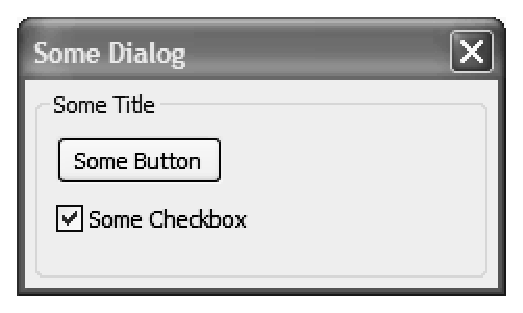
\includegraphics[width={150pt}]{../images/audacity/SomeDialog.eps}
\end{minipage}
%% \caption{Example Dialog}
\caption{ダイアログの例}
\label{fig.aud.2}
\end{figure}

%% This code defines a static box in a dialog and that box contains a
%% button and a checkbox.  The correspondence between the code and the
%% dialog should be clear.  The \code{StartStatic} and \code{EndStatic}
%% are paired calls.  Other similar
%% \code{StartSomething}/\code{EndSomething} pairs, which must match, are
%% used for controlling other aspects of layout of the dialog.  The curly
%% brackets and the indenting that goes with them aren't needed for this
%% to be correct code.  We adopted the convention of adding them in to
%% make the structure and particularly the matching of the paired calls
%% obvious.  It really helps readability in larger examples.
このコードはダイアログ内に静的なボックスを定義し、その中にボタンとチェックボックスをひとつずつ置いている。コードとダイアログの対応は明確だ。\code{StartStatic}と\code{EndStatic}の呼び出しはペアになっている。それ以外にも同様な\code{StartSomething}/\code{EndSomething}のペアがあり、これらは必ずセットで存在しなければならない。これが、ダイアログ上の配置を制御する。波括弧での囲みやその中の字下げは単にコードの見た目だけにかかわるものであり、必須というわけではない。しかし我々は、このように書くよう規約を定めている。コードの構造や\code{StartSomething}/\code{EndSomething}のペアを明確にするためである。コードが巨大になってくると、これが可読性の向上にとても役立つ。

%% The source code shown does not just create the dialog.  The code after
%% the comment ``\code{//GUI Structure}'' can also be used to shuttle
%% data from the dialog out to where the user preferences are stored, and
%% to shuttle data back in.  Previously a lot of the repetitive code came
%% from the need to do this.  Nowadays that code is only written once and
%% is buried within the \code{ShuttleGui} class.
先ほど示したソースコードは、単にダイアログを作るだけではない。コメント``\code{//GUI Structure}''の後に続くコードを使って、ダイアログのデータを設定保存先に送ったり逆にデータを取得したりすることができる。これまでは、同様のことをするためには、同じようなコードを大量に繰り返さねばならなかった。今では、コードを一度だけ書けばあとは\code{ShuttleGui}クラスがうまくやってくれる。

%% There are other extensions to the basic wxWidgets in Audacity.
%% Audacity has its own class for managing toolbars.  Why doesn't it use
%% wxWidget's built in toolbar class?  The reason is historic: Audacity's
%% toolbars were written before wxWidgets provided a toolbar class.
それ以外にもAudacityでは、wxWidgetsの基本機能を拡張するモジュールを使っている。たとえば、Audacityにはツールバーを管理するための自前のクラスがある。なぜwxWidgetの組み込みのツールバークラスを使わなかったのかって?それは、歴史的な理由によるものだ。Audacityのツールバーが書かれたのは、wxWidgetsにツールバークラスが用意されるよりも前のことだったのだ。

\end{aosasect1}

%% \begin{aosasect1}{The TrackPanel}
\begin{aosasect1}{TrackPanel}

%% The main panel in Audacity which displays audio waveforms is the
%% TrackPanel.  This is a custom control drawn by Audacity.  It's made up
%% of components such as smaller panels with track information, a ruler
%% for the timebase, rulers for amplitude, and tracks which may show
%% waveforms, spectra or textual labels.  The tracks can be resized and
%% moved around by dragging.  The tracks containing textual labels make
%% use of our own re-implementation of an editable text box rather than
%% using the built-in text box.  You might think these panels tracks and
%% rulers should each be a wxWidgets component, but they are not.
Audacityのメインパネルで波形を表示しているのがTrackPanelで、これはAudacityのカスタムコントロールだ。このコントロールは、いくつかの小さな部品を組み合わせて作られている。トラック情報を表示するパネルや時間軸のルーラー、振幅のルーラー、そしてトラックの波形やテキストラベルなどだ。トラックのサイズ変更や移動は、マウスのドラッグで行える。トラックにはテキストラベルが含まれているが、これは編集可能なテキストボックスを自前で再実装したものであり、組み込みのテキストボックスではない。これらのパネルやトラック、ルーラーはwxWidgetsのコンポーネントにすべきだと考える人もいるだろう。しかしそのようにはなっていない。

%% \aosafigure{../images/audacity/MainPanelAnnotated.eps}{Audacity Interface with Track Panel Elements Labelled}{fig.aud.3}
\aosafigure{../images/audacity/MainPanelAnnotated.eps}{Audacityのインターフェイスに、Track Panelの要素名を示したもの}{fig.aud.3}

%% The screenshot shown in \aosafigref{fig.aud.3} shows the Audacity user
%% interface.  All the components that have been labelled are custom for
%% Audacity.  As far as wxWidgets is concerned there is one wxWidget
%% component for the TrackPanel.  Audacity code, not wxWidgets, takes
%% care of the positioning and repainting within that.
スクリーンショット\aosafigref{fig.aud.3}にAudacityのユーザーインターフェイスを示す。名前がつけられているコンポーネントはすべて、Audacity用にカスタマイズしたものである。wxWidgetsの観点から見れば、ここにあるwxWidgetのコンポーネントはTrackPanel用のひとつだけだ。その内部の配置や再描画はすべて、wxWidgetではなくAudacity側のコードが面倒を見ている。

%% The way all these components fit together to make the TrackPanel is
%% truly horrible.  (It's the code that's horrible; the end result the
%% user sees looks just fine.)  The GUI and application-specific code is
%% all mixed together, not separated cleanly.  In a good design only our
%% application-specific code should know about left and right audio
%% channels, decibels, muting and soloing.  GUI elements should be
%% application agnostic elements that are reusable in a non-audio
%% application.  Even the purely GUI parts of TrackPanel are a patchwork
%% of special case code with absolute positions and sizes and not enough
%% abstraction.  It would be so much nicer, cleaner and more consistent
%% if these special components were self-contained GUI elements and if
%% they used sizers with the same kinds of interface as wxWidgets uses.
これらのコンポーネントをうまく取りまとめてTrackPanelを作るのは、本当に恐ろしいことだ(恐ろしいのはあくまでもコードのことであって、実際にユーザーが使う完成品はよくできているけどね)。GUIとアプリケーションのコードが入り混じっていて、きれいに分離できていない。きちんと設計するなら、アプリケーションのコードだけが左右のオーディオチャンネルやそのデシベル、ミュート、ソロなどの設定を関知するべきだ。GUIの要素がそれらを関知しているようではいけない。GUIの要素はオーディオ関連以外のアプリケーションでも再利用可能でなければならない。TrackPanel上の部品は、純粋なGUIでさえもつぎはぎだらけのコードになっている。絶対位置やサイズによる場合分けが含まれており、十分に抽象化できていない。これらのコンポーネントが自身でGUI要素を内包してwxWidgetsのsizerのようなインターフェイスを使っていれば、どんなにきれいで一貫性のあるコードになるだろう。

%% To get to such a TrackPanel we'd need a new sizer for wxWidgets that
%% can move and resize tracks or, indeed, any other widget.  wxWidgets
%% sizers aren't yet that flexible.  As a spin off benefit we could use
%% that sizer elsewhere.  We could use it in the toolbars that hold the
%% buttons, making it easy to customize the order of buttons within a
%% toolbar by dragging.
TrackPanelをそんなふうに改良するために、トラックやその他のウィジェットの移動やサイズ変更を行うwxWidgets用の新たなsizerが必要となった。wxWidgetsのsizerは、それを満たすほど柔軟ではない。新たにsizerを作ったおかげで、それを他の部分でも使えるようになった。我々はツールバー上に保持するボタンにもこれを使い、ツールバー上のボタンの並べ替えをドラッグで簡単にできるようにした。

%% Some exploratory work has been done in creating and using such sizers,
%% but not enough.  Some experiments with making the GUI components fully
%% fledged wxWidgets ran into a problem: doing so reduces our control
%% over repainting of the widgets, resulting in flicker when resizing and
%% moving components.  We would need to
%% extensively modify wxWidgets to achieve flicker-free repainting, and
%% better separate the resizing steps from the repainting steps.
新たなsizerを作るために事前調査を行ったが、調査が足りなかったようだ。GUIコンポーネントをwxWidgetsから完全に独立させようとする試みたが、問題が発生した。ウィジェットの再描画がうまく制御できなくなり、コンポーネントのサイズを変更したり移動させたりするとちらつきが発生するようになったのだ。wxWidgetsをベースにして拡張することで再描画時のちらつきを解決し、サイズ変更の処理と再描画の処理をうまく分離させる必要があった。

%% A second reason to be wary of this approach for the TrackPanel is that
%% we already know wxWidgets start running very slowly when there are
%% large numbers of widgets.  This is mostly outside of wxWidget's
%% control.  Each wxWidget, button, and text entry box uses a
%% resource from the windowing system. Each has a handle to access it.
%% Processing large numbers of these takes time.  Processing is slow even
%% when the majority of widgets are hidden or off screen.  We want to be
%% able to use many small widgets on our tracks.
TrackPanelをこの方式で改良するのを躊躇したもうひとつの理由は、ウィジェット数が増えるとwxWidgetsの起動に時間がかかることを既に我々が知っていたからだ。これは、wxWidgetsからはあまり手の施しようのない問題だ。個々のwxWidgetやボタン、テキスト入力ボックスはそれぞれウィンドウシステムのリソースを使っている。そして、個々のリソースは、アクセスするためのハンドルを持っている。多数のハンドルを処理するのには時間がかかる。たとえ大半のウィジェットが非表示あるいはスクリーンの外部にある場合であっても処理が遅くなることは変わらない。我々は、小さなウィジェットを大量に使うつもりだったのだ。

%% The best solution is to use a flyweight pattern, lightweight
%% widgets that we draw ourselves, which do not have corresponding
%% objects that consume windowing system resources or handles.  We would
%% use a structure like wxWidgets's sizers and component widgets, and
%% give the components a similar API but not actually derive from
%% wxWidgets classes.  We'd be refactoring our existing TrackPanel code
%% so that its structure became a lot clearer.  If this were an easy
%% solution it would already have been done, but diverging opinions about
%% exactly what we want to end up with derailed an earlier attempt.
%% Generalizing our current ad hoc approach would take significant design
%% work and coding.  There is a great temptation to leave complex code
%% that already works well enough alone.
最もよい解決策はFlyweightパターンを採用することだ。軽量なウィジェットが自分自身の描画を担当し、対応するオブジェクトを持たないようにすれば、ウィンドウシステムのリソースやハンドルを消費せずに済む。我々はwxWidgetsのsizerやコンポーネントウィジェットと同様の構造を使い、同様のAPIを提供するようにした。しかしそれはwxWidgetsのクラス群を派生させたものではない。我々は既存のTrackPanelのコードをリファクタリングでよりきれいな構造にした。もしこれが簡単な解決法なら既にそうしていただろうが、自分たちがいったい何を求めているのかについての議論が発散した結果、初期の試みから脱線してしまった。現在のアドホックな方式を一般化するには、大変な設計作業とコーディングが必要となる。複雑ではあるけれども今きちんと動いているコードをそのまま残しておきたいという強い誘惑にもかられた。

\end{aosasect1}

%% \begin{aosasect1}{PortAudio Library: Recording and Playback}
\begin{aosasect1}{PortAudioライブラリ: 録音と再生}

%% PortAudio is the audio library that gives Audacity the ability to play
%% and record audio in a cross-platform way.  Without it Audacity would
%% not be able to use the sound card of the device it's running on.
%% PortAudio provides the ring
%% buffers, sample rate conversion when playing/recording and, crucially,
%% provides an API that hides the differences between audio on Mac, Linux
%% and Windows.  Within PortAudio there are alternative implementation
%% files to support this API for each platform.
PortAudioはオーディオライブラリで、Audacityはこれを使って、録音と再生をクロスプラットフォームな方法で提供している。このライブラリがなければ、Audacityは実行環境のサウンドカードを使うことができないだろう。PortAudioが提供する機能にはリングバッファや録音・再生時のサンプルレート変換などがある。重要なのは、そのAPIによってMacやLinuxそしてWindowsにおけるオーディオ処理の差異を隠ぺいできるということだ。PortAudioの内部には、各プラットフォームでAPIに対応するための実装ファイルが別々に用意されている。

%% I've never needed to dig into PortAudio to follow what happens inside.
%% It is, however, useful to know how we interface with PortAudio.
%% Audacity accepts data packets from PortAudio (recording) and sends
%% packets to PortAudio (playback).  It's worth looking at
%% exactly how the sending and
%% receiving happens, and how it fits in with reading and writing to disk
%% and updates to the screen.
私はこれまで、PortAudioの内部に立ち入って何をしているのか追いかける必要などなかった。しかし、AudacityとPortAudioの間でどのようなやりとりをしているかを知っておくと便利だ。Audacityは、PortAudioからデータのパケットを受信(録音)したり、逆にパケットをPortAudioに送信(再生)したりする。送信や受信が実際のところどのように行われているのか、そしてそれがディスクへの読み書きや描画の更新とどのようにつながっているのか。そのあたりは見る価値があるだろう。

%% Several different processes are going on at the same time.  Some
%% happen frequently, transfer small amounts of data, and must be
%% responded to quickly.  Others happen less frequently, transfer larger
%% quantities of data, and the exact timing of when they happen is less
%% critical.  This is an impedance mismatch between the processes,
%% and buffers are used to accommodate it.  A second part of the picture is
%% that we are dealing with audio devices, hard drives,
%% and the screen.  We don't go down to the wire and so have to work with
%% the APIs we're given.  Whilst we would like each of our processes to
%% look similar, for example to have each running from a wxThread, we
%% don't have that luxury (\aosafigref{fig.aud.4}).
いくつかの異なる処理が、同時に発生する。頻繁に発生し、少量のデータをやりとりし、高速な反応を要するものがあれば、あまり頻繁には発生しないが大量のデータをやりとりしなければならないものもある。こちらについては処理がいつ発生するかはそれほど重要ではない。ここに、処理の内容とその対応に使うバッファとの間のインピーダンスミスマッチが発生する。もうひとつ見る価値があるのは、オーディオデバイスやハードディスクそして表示画面などを扱う部分だ。末端まで必死になって追いかけるつもりはなく、与えられたAPIを使って作業をすることになる。各プロセスを同じように見て、たとえばすべてwxThreadから立ち上げるようにしたいものだが、そのような贅沢はできない(\aosafigref{fig.aud.4})。

%% \aosafigureTop[325pt]{../images/audacity/Buffers.eps}{Threads and Buffers in Playback and Recording}{fig.aud.4}
\aosafigureTop[325pt]{../images/audacity/Buffers.eps}{録音・再生時のスレッドとバッファ}{fig.aud.4}

%% One audio thread is started by PortAudio code and interacts directly
%% with the audio device.  This is what drives recording or playback.
%% This thread has to be responsive or packets will get lost.  The
%% thread, under the control of PortAudio code, calls
%% \code{audacityAudioCallback} which, when recording, adds newly arrived
%% small packets to a larger (five second) capture buffer.  When playing
%% back it takes small chunks off a five second playback buffer.  The
%% PortAudio library knows nothing about wxWidgets and so this thread
%% created by PortAudio is a pthread.
ひとつのオーディオスレッドをPortAudioのコードが立ち上げ、それが直接オーディオデバイスとやりとりする。これは、録音や再生を行うものだ。このスレッドは反応が速いものでなければならず、そうでないとパケットを失ってしまう。PortAudioのコードの配下にあるスレッドが\code{audacityAudioCallback}を呼び、録音時には、新たに受け取った小さなパケットを大きめ(5秒)のキャプチャバッファに追加する。再生時には、5秒間の再生バッファから小さな塊を取り出す。PortAudioライブラリはwxWidgetsについては一切知らない。そのため、PortAudioが作ったこのスレッドはpthreadである。

%% A second thread is started by code in Audacity's class AudioIO\@.  When
%% recording, AudioIO takes the data from the capture buffer and appends
%% it to Audacity's tracks so that it will eventually get displayed.
%% Additionally, when enough data has been added, AudioIO writes the data
%% to disk.  This same thread also does the disk reads for audio
%% playback.  The function \code{AudioIO::FillBuffers} is the key
%% function here and depending on the settings of some Boolean variables,
%% handles both recording and playback in the one function.  It's
%% important that the one function handle both directions.  Both the
%% recording and playback parts are used at the same time when doing
%% ``software play through,'' where you overdub what was previously
%% recorded.  In the AudioIO thread we are totally at the mercy of the
%% operating system's disk IO\@.  We may stall for an unknown length of
%% time reading or writing to a disk.  We could not do those reads or
%% writes in \code{audacityAudioCallback} because of the need to be
%% responsive there.
第二のスレッドを立ち上げるのは、AudacityのAudioIO\@クラスだ。録音の際に、AudioIOがデータをキャプチャバッファから受け取り、それをAudacityのトラックに追加して表示させる。さらに、十分な量のデータが追加された時点で、AudioIOがデータをディスクに書き込む。このスレッドは、再生時のディスクからの読み込みも行う。ここで鍵となるのが関数\code{AudioIO::FillBuffers}といくつかのBoolean変数の設定で、録音と再生をこのひとつの関数で行う。重要なのは、このひとつの関数で双方向の処理をしているということだ。録音部と再生部を同時に使うことがある。``software play through''で、以前に録音された内容に対する多重録音を行うときだ。AudioIOのスレッド内では、完全にOSのディスクIO\@にしばられた状態となり、ディスクの読み書きでしばらく待たされることもあるかもしれない。これらの読み書きを\code{audacityAudioCallback}で行うことはできない。この関数は高速な反応を要求されるからである。

%% Communication between these two threads happens via shared variables.
%% Because we control which threads are writing to these variables and
%% when, we avoid the need for more expensive mutexes.
これらふたつのスレッド間の通信は、共有変数を使って行う。どちらの変数がいつ書き込みを行っているのかを制御できているので、ミューテックスを使うようなぜいたくは不要だ。

\pagebreak

%% In both playback and recording, there is an additional requirement:
%% Audacity also needs to update the GUI\@.  This is the least time
%% critical operation.  The update happens in the main GUI thread and is
%% due to a periodic timer that ticks twenty times a second.  This
%% timer's tick causes \code{TrackPanel::OnTimer} to be called, and if
%% updates to the GUI are found to be needed, they are applied.  This
%% main GUI thread is created within wxWidgets rather than by our own
%% code.  It is special in that other threads cannot directly update the
%% GUI\@.  Using a timer to get the GUI thread to check if it needs to
%% update the screen allows us to reduce the number of repaints to a
%% level that is acceptable for a responsive display, and not make too
%% heavy demands on processor time for displaying.
再生と録音の両方で、さらにもうひとつの要件がある。AudacityはGUI\@も更新しなければならないということだ。これは、最もタイムクリティカルでない処理である。描画の更新はメインのGUIスレッドで行われ、1秒間に20回発生する定期的なタイマーで実行される。このタイマーが\code{TrackPanel::OnTimer}を呼び出し、GUIの更新が必要な場所が見つかれば更新する。メインのGUIスレッドは、我々のコードではなくwxWidgetsの中から立ち上げる。他のスレッドからは、直接GUI\@を更新することはできない。タイマーを使ってGUIスレッドを取得し、画面の更新が必要かどうかを調べる。そうすることで、再描画の回数を減らしながらも許容できるレベルの反応を保つ。また、そうすることで、表示用にあまりプロセッサタイムを要求しすぎないようにしている。

%% Is it good design to have an audio device thread, a buffer/disk thread
%% and a GUI thread with periodic timer to handle these audio data
%% transfers?  It is somewhat ad hoc to have these three different
%% threads that are not based on a single abstract base class.  However,
%% the ad-hockery is largely dictated by the libraries we use.  PortAudio
%% expects to create a thread itself.  The wxWidgets framework
%% automatically has a GUI thread.  Our need for a buffer filling thread
%% is dictated by our need to fix the impedance mismatch between the
%% frequent small packets of the audio device thread and the less
%% frequent larger packets of the disk drive.  There is very clear
%% benefit in using these libraries.  The cost in using the libraries is
%% that we end up using the abstractions they provide.  As a result we
%% copy data in memory from one place to another more than is strictly
%% necessary.  In fast data switches I've worked on, I've seen extremely
%% efficient code for handling these kinds of impedance mismatches
%% that is interrupt driven and does not use threads at all.  Pointers to
%% buffers are passed around rather than copying data.  You can only do
%% that if the libraries you are using are designed with a richer buffer
%% abstraction.  Using the existing interfaces, we're forced to use
%% threads and we're forced to copy data.
オーディオデバイス用のスレッドとバッファ/ディスク用のスレッド、そして定期的なタイマーを持つGUIスレッドの三つを使ってオーディオデータのやりとりをするというのは、よい設計と言えるだろうか?これら三種類のスレッドを単一の抽象基底クラスから派生させないのは、多少アドホックにも感じる。しかし、このアドホック性の要因の多くは、使っているライブラリによるものである。PortAudioは、自分自身でスレッドを作ることを想定している。wxWidgetsフレームワークがGUIスレッドを持っているのは、ごく自然なことだ。バッファを埋めるためのスレッドを要する理由は、オーディオデバイスのスレッドで頻繁に発生する小規模のパケットと、あまり頻繁には発生しないディスクドライブの大規模なパケットとの間のインピーダンスミスマッチを解決するためだ。これらのライブラリを使うことには明確な利点がある。逆に、これらのライブラリを使うことで必要となるコストは、結局は各ライブラリが提供する抽象化を使うことになるということだ。結果的に、メモリ内でのデータのコピーの回数が、最低限必要な回数だけでなくさらに増えてしまっている。私がこれまで関わってきた高速なデータ交換の処理ではもっと効率的なコードを見たことがある。そのコードでは、割り込みなどで発生するこの手のインピーダンスミスマッチに対応するのにスレッドなど使っていなかった。データをコピーするのではなく、バッファへのポインタを渡していたのだ。ただ、そんなことができるのは、使っているライブラリがバッファの抽象化をよりリッチに設計している場合だけである。既存のインターフェイスを使う限りはスレッドを使うことを強いられ、そしてデータのコピーを強いられることになる。

\end{aosasect1}

%% \begin{aosasect1}{BlockFiles}
\begin{aosasect1}{BlockFile}

%% One of the challenges faced by Audacity is supporting insertions and
%% deletions into audio recordings that may be hours long.  Recordings
%% can easily be too long to fit in available RAM\@.  If an audio recording
%% is in a single disk file, inserting audio somewhere near the start of
%% that file could mean moving a lot of data to make way.  Copying that
%% data on disk would be time consuming and mean that Audacity could then
%% not respond rapidly to simple edits.
Audacityが直面する困難のひとつが、録音したオーディオデータへのデータの追加や削除だ。オーディオデータの長さは数時間分になることもある。録音データはどんどん長くなり、利用可能なRAM\@の容量を簡単に突破してしまうだろう。録音データをディスク上に単一のファイルとして管理していたとすると、ファイルの先頭あたりにデータを挿入しようとしたときには大量のデータ移動が発生することになる。ディスク上でのデータのコピーには時間がかかる。つまり、Audacityはちょっとした編集でも長々と待たされるソフトウェアになってしまう。

%% Audacity's solution to this is to divide audio files into many
%% BlockFiles, each of which could be around 1 MB\@.  This is the main
%% reason Audacity has its own audio file format, a master file with the
%% extension \code{.aup}.  It is an XML file which coordinates the various
%% blocks.  Changes near the start of a long audio recording might affect
%% just one block and the master \code{.aup} file.
Audacityがこの問題に対処するために使った方法は、オーディオファイルを多数のBlockFileに分割することだ。個々のファイルの大きさは約1 MB\@となる。これが、Audacityが自前のオーディオファイルフォーマットを採用している主な理由だ。マスターファイルの拡張子は\code{.aup}となる。これはXMLファイルで、このファイルがさまざまなブロックを取りまとめている。長いオーディオデータの先頭近くを変更した場合でも、影響を受けるのはたったひとつのブロックとマスターファイル\code{.aup}だけとなる。

%% BlockFiles balance two conflicting forces.  We can insert and delete
%% audio without excessive copying, and during playback we are guaranteed
%% to get reasonably large chunks of audio with each request to the disk.
%% The smaller the blocks, the more potential disk requests to fetch the
%% same amount of audio data; the larger the blocks, the more copying on
%% insertions and deletions.
BlockFileは、対立する二つの勢力の調和をうまく保っている。挿入や削除の際に必要以上のコピーが発生することもないし、再生時には、ディスクへのリクエストのたびに適度に大きなデータの塊を取得できることが保証されている。ブロックが小さくなればなるほど、同じ量のオーディオデータを取得するために必要なディスクへのリクエストの回数が増え、逆に大きくなればなるほど挿入や削除の際のコピーの量が増える。

%% Audacity's BlockFiles never have internal free space and they never
%% grow beyond the maximum block size.  To keep this true when we insert
%% or delete we may end up copying up to one block's worth of data.  When
%% we don't need a BlockFile anymore we delete it.  The BlockFiles are
%% reference counted so if we delete some audio, the relevant BlockFiles
%% will still hang around to support the undo mechanism until we save.
%% There is never a need to garbage collect free space within
%% Audacity BlockFiles, which we would need to do with an all-in-one-file
%% approach.
AudacityのBlockFileは決して内部に空き領域を持たないし、最大のブロックサイズを超えることもない。このルールを守るため、挿入や削除をするときには最大1ブロックまでのデータのコピーが発生する可能性がある。BlockFileが不要になれば、削除する。BlockFileは参照カウンタで管理されているので、オーディオの一部を削除したとしてもそれに関連するBlockFileはまだ残ったままであり、undoに対応できるようにしている。データを保存するまではその状態になる。AudacityのBlockFileには、空き領域のガベージコレクションはまったく不要だ。我々が対応する必要があるのは、オールインワン型のファイルである。

%% Merging and splitting larger chunks of data is the bread and butter of
%% data management systems, from B-trees to Google's BigTable tablets to
%% the management of unrolled linked lists.  \aosafigref{fig.aud.5} shows
%% what happens in Audacity when removing a span of audio near the start.
大きめのデータのマージや分割こそが、データを管理するシステムの本業である。BツリーからGoogleのBigTableのタブレットやUnrolled linked listの管理まで、それは変わらない。\aosafigref{fig.aud.5}は、Audacityでオーディオの開始位置付近を削除したときに何が起こるのかを示している。

%% \aosafigure[200pt]{../images/audacity/BlocksCombined.eps}{Before deletion, \code{.aup} file and BlockFiles hold the sequence ABCDEFGHIJKLMNO. After deletion of FGHI, two BlockFiles are merged.}{fig.aud.5}
\aosafigure[200pt]{../images/audacity/BlocksCombined.eps}{削除する前は\code{.aup}ファイルとBlockFileが保持するのはABCDEFGHIJKLMNO。FGHIを削除すると、ふたつのBlockFileがマージされる。}{fig.aud.5}

%% BlockFiles aren't just used for the audio itself.  There are also
%% BlockFiles that cache summary information.  If Audacity is asked to
%% display a four hour long recording on screen it is not acceptable for
%% it to process the entire audio each time it redraws the screen.
%% Instead it uses summary information which gives the maximum and
%% minimum audio amplitude over ranges of time.  When zoomed in,
%% Audacity is drawing using actual samples.  When zoomed out,
%% Audacity is drawing using summary information.
BlockFileが扱うのはオーディオそのものだけではない。それ以外にも、サマリ情報をキャッシュするBlockFileもある。Audacityで4時間のオーディオデータを表示するときに、画面の再描画のたびにオーディオ全体を読み直すのは考えられない話だ。そういう場合にサマリ情報を代わりに使う。サマリ情報には、その時間の範囲内での最大音量や最小音量が記録されている。表示をズームインしたときは、実際のデータを使って描画を行い、ズームアウトしたときはサマリ情報をもとに描画を行う。

%% A refinement in the BlockFile system is that the blocks needn't be
%% files created by Audacity.  They can be references to subsections of
%% audio files such as a timespan from audio stored in the \code{.wav} format.
%% A user can create an Audacity project, import audio from a \code{.wav} file
%% and mix a number of tracks whilst only creating BlockFiles for the
%% summary information.  This saves disk space and saves time in copying
%% audio.  All told it is, however, a rather bad idea.  Far too many of
%% our users have removed the original audio \code{.wav} file thinking there
%% will be a complete copy in the Audacity project folder.  That's not so
%% and without the original \code{.wav} file the audio project can no longer be
%% played.  The default in Audacity nowadays is to always copy imported
%% audio, creating new BlockFiles in the process.
BlockFileシステムの特徴のひとつに、各ブロックはAudacityが作ったファイルでなくてもかまわないという点がある。たとえば、\code{.wav}形式で保存されたオーディオファイルの特定の時間範囲を指すこともできる。ユーザーがAudacityプロジェクトを立ち上げて\code{.wav}ファイルからオーディオをインポートしていくつかのトラックをミックスしたとしよう。このときに作られるBlockFileはサマリ情報を格納するものだけだ。そのおかげでディスク容量も抑えられるし、オーディオデータをコピーする時間も節約できる。しかしながら、これはあまり良い考えではない。これまでに、多くのユーザーがインポート後に元の\code{.wav}ファイルを削除してしまっていた。Audacityのプロジェクトフォルダに全部コピーされているものと勘違いしていたのだ。実際はそうではなく、元の\code{.wav}ファイルがなければそのプロジェクトは再生できない。そのため、Audacityの現在のデフォルト設定では、インポートしたオーディオを常にコピーして新しいBlockFileを作るようにしている。

%% The BlockFile solution ran into problems on Windows systems where
%% having a large number of BlockFiles performed very poorly.  This appeared
%% to be because Windows was much slower handling
%% files when there were many in the same directory, a similar problem to
%% the slowdown with large numbers of widgets.  A later addition was made
%% to use a hierarchy of subdirectories, never with more than a hundred
%% files in each subdirectory.
BlockFile方式が、Windows上で問題となることがあった。Windows上で大量のBlockFileを扱うと、パフォーマンスが非常に劣化したのだ。原因はおそらく、Windowsでは同一ディレクトリ上にある大量のファイルの処理速度に難があったからだろう。同様の問題が、ウィジェットをたくさん使ったときの速度低下という形でもあらわれた。その後、サブディレクトリ階層を使うように変更を加え、ひとつのディレクトリには最大100個までのファイルしか置かないようにした。

%% The main problem with the BlockFile structure is that it is exposed to
%% end users.  We often hear from users who move the \code{.aup} file and don't
%% realize they also need to move the folder containing all the
%% BlockFiles too.  It would be better if Audacity projects were a single
%% file with Audacity taking responsibility for how the space inside the
%% file is used.  If anything this would increase performance rather than
%% reduce it.  The main additional code needed would be for garbage
%% collection.  A simple approach to that would be to copy the blocks to
%% a new file when saving if more than a set percentage of the file were
%% unused.
BlockFileの構造を使うときの最大の問題は、その構造がエンドユーザーに公開されてしまうことだ。よく聞く話だが、\code{.aup}ファイルを別の場所に移したユーザーが、BlockFileを含むフォルダも一緒に移動させなければならないことに気付かないということがある。Audacityのプロジェクトが単一のファイルにまとまっていて、その内部のスペースやファイル内の利用状況を管理できる状態であればよかっただろう。こうすれば、パフォーマンスはどちらかといえば向上するだろう。追加で必要となるコードは、おそらくガベージコレクションであろう。シンプルなアプローチとしては、ファイルのみ使用領域が設定した割合を上回るときにブロックを新しいファイルへコピーするという方法がある。

\end{aosasect1}

%% \begin{aosasect1}{Scripting}
\begin{aosasect1}{スクリプト}

%% Audacity has an experimental plugin that supports multiple scripting
%% languages.  It provides a scripting interface over a named pipe.  The
%% commands exposed via scripting are in a textual format, as are the
%% responses.  As long as the user's scripting language can write text to
%% and read text from a named pipe, the scripting language can drive
%% Audacity.  Audio and other high-volume data does not need to travel on
%% the pipe (\aosafigref{fig.aud.7}).
Audacityには、複数のスクリプト言語に対応する実験的なプラグインが付属している。このプラグインは、名前付きパイプを使ったスクリプトインターフェイスを提供する。スクリプト用に公開されたコマンドはテキスト形式で、同じくコマンドの応答もテキストとなる。つまり、名前付きパイプへのテキストの書き出しや名前付きパイプからのテキストの読み込みに対応しているスクリプト言語ならなんでも、Audacityを動かせるということだ。オーディオそのものなどの大きなデータにパイプ上を行き来させる必要はない(\aosafigref{fig.aud.7})。

%% \aosafigure[75pt]{../images/audacity/Scripting.eps}{Scripting Plugin Provides Scripting Over a Named Pipe}{fig.aud.7}
\aosafigure[75pt]{../images/audacity/Scripting.eps}{スクリプトプラグインが、名前付きパイプを使ったスクリプト処理機能を提供する}{fig.aud.7}

%% The plugin itself knows nothing about the content of the text traffic
%% that it carries. It is only responsible for conveying it. The plugin
%% interface (or rudimentary extension point) used by the scripting
%% plugin to plug in to Audacity already exposes Audacity commands in
%% textual format.  So, the scripting plugin is small, its main content
%% being code for the pipe.
プラグイン自身は、自分が運ぶテキストの内容については何も知らない。単にそれを運ぶだけだ。スクリプトプラグインが使うプラグインインターフェイス(あるいは原始的な拡張ポイント)は、Audacity側でテキスト形式のコマンドとして公開されている。そのため、スクリプトプラグインは小さなプラグインで、コードの大部分はパイプを扱う処理である。

%% Unfortunately a pipe introduces similar security risks to having a
%% TCP/IP connection---and we've ruled out TCP/IP connections for
%% Audacity on security grounds.  To reduce that risk the plugin is an
%% optional DLL\@.  You have to make a deliberate decision to obtain and
%% use it and it comes with a health/security warning.
残念ながら、パイプを使うということはTCP/IP接続を扱うのと同じセキュリティリスクを負うことになる---セキュリティを考慮してAudacityではTCP/IP接続を扱わないことに決めている。リスクを少しでも下げるために、このプラグインはオプションのDLL\@としている。これを取得して使う前には熟考が必要だ。また、このプラグインを使うときにはセキュリティに関する警告が出る。

%% After the scripting feature had already been started, a suggestion
%% surfaced in the feature requests page of our wiki that we should
%% consider using KDE's D-Bus standard to provide an inter-process call
%% mechanism using TCP/IP\@.  We'd already started going down a different
%% route but it still might make sense to adapt the interface we've ended
%% up with to support D-Bus.
スクリプトの機能を公開した後で、Wikiの機能追加リクエストのページでこんな提案を受けた。KDEのD-Busを使えばTCP/IP\@によるプロセス間通信機能を提供できるのではないか、というものだ。既に別のやりかたで始めたところではあるが、最終的にD-Busをサポートするようになる可能性も残っている。

%% \begin{aosabox}{Origins of Scripting Code}
\begin{aosabox}{スクリプト機能のはじまり}

%% The scripting feature grew from an enthusiast's adaptation of Audacity
%% for a particular need that was heading in the direction of being a
%% fork.  These features, together called CleanSpeech, provide for mp3
%% conversion of sermons.  CleanSpeech adds new effects such as truncate
%% silence---the effect finds and cuts out long silences in audio---and
%% the ability to apply a fixed sequence of existing noise removal
%% effects, normalization and mp3 conversion to a whole batch of audio
%% recordings.  We wanted some of the excellent functionality in this,
%% but the way it was written was too special case for Audacity.
%% Bringing it into mainstream Audacity led us to code for a flexible
%% sequence rather than a fixed sequence.  The flexible sequence could
%% use any of the effects via a look-up table for command names and a
%% \code{Shuttle} class to persist the command parameters to a textual
%% format in user preferences.  This feature is called \emph{batch
%% chains}.  Very deliberately we stopped short of adding conditionals
%% or calculation to avoid inventing an ad hoc scripting language.
スクリプト機能ができたきっかけは、あるAudacityファンから提供された機能だった。それはあるニーズを満たすための機能で、当初はAudacityをフォークする方向に向かっていた。その機能はひとまとめにしてCleanSpeechと呼ばれ、教会での説教をmp3に変換するために作られた。CleanSpeechには無音部分の切り詰め---オーディオ内の長い無音部分を探して切り取る---などの新たなエフェクトやノイズ除去効果のある固定シーケンスを適用する機能があり、オーディオの正規化や録音内容のmp3への変換機能などもあった。中にはぜひ取り込みたくなるような素晴らしい機能もあったが、その実装はAudacity内ではかなり特殊なものだった。それをAudacityの本流に取り込むと、固定シーケンスではなく可変シーケンスのコードを書くことになった。可変シーケンスだと、コマンド名と\code{Shuttle}クラスのルックアップテーブル経由で任意のエフェクトを使い、コマンドのパラメータはテキスト形式でユーザー設定項目に格納することができた。この機能は\emph{バッチチェイン}と名付けられた。条件分岐や計算式を追加して楽をすることを意図的に避け、アドホックなスクリプト言語を作ってしまわないようにした。

%% In retrospect the effort to avoid a fork has been well worthwhile.
%% There is still a CleanSpeech mode buried in Audacity that can be
%% set by modifying a preference. It also cuts down the user interface,
%% removing advanced features. A simplified version of Audacity has been
%% requested for other uses, most notably in schools. The problem is that
%% each person's view of which are the advanced features and which are
%% the essential ones is different.  We've subsequently implemented a
%% simple hack that leverages the translation mechanism.  When the
%% translation of a menu item starts with a ``\#'' it is no longer shown
%% in the menus.  That way people who want to reduce the menus can make
%% choices themselves without recompiling---more general and less
%% invasive than the \code{mCleanspeech} flag in Audacity, which in time we
%% may be able to remove entirely.
今にして思えば、フォークを避けようと努力をする価値はあった。今でもCleanSpeechモードはAudacityに埋め込まれており、環境設定で有効にすることができる。さらにユーザーインターフェイスも減らし、高度な機能は削除した。シンプルにしたバージョンのAudacityは、他の用途で使いたいという要望もくるようになった。中でも特筆すべきなのは学校での採用だった。問題は、どれが高度な機能でどれが必要不可欠な機能なのかについての意見が人によって異なっていたということだ。我々はその後シンプルなハックを行い、翻訳の仕組みを向上させた。メニュー項目の翻訳のうち``\#''で始まるものは、メニューに表示しないようにしたのだ。これで、メニューの項目が多すぎると感じる人も再コンパイルなしでメニューを減らせるようになった---これはより汎用的であり、Audacityの\code{mCleanspeech}フラグほどには侵略的ではない。このフラグは、いつか取り除いてしまいたいものだ。

%% The CleanSpeech work gave us batch chains and the ability to
%% truncate silence.  Both
%% have attracted additional improvement from outside the core team.
%% Batch chains directly led on to the scripting feature.  That in turn
%% has begun the process of supporting more general purpose plugins to
%% adapt Audacity.
CleanSpeechの作業は、我々にバッチチェインと無音切り詰め機能をもたらした。どちらも、コアチーム以外から持ち込まれた魅力的な機能改善だ。バッチチェインはその後のスクリプト機能につながった。それはまた、より汎用的なプラグイン機能をAudacityに持ち込むきっかけにもなった。

\end{aosabox}

\end{aosasect1}

%% \begin{aosasect1}{Real-Time Effects}
\begin{aosasect1}{リアルタイムエフェクト}

%% Audacity does not have real-time effects, that is, audio effects that
%% are calculated on demand as the audio plays.  Instead in Audacity you
%% apply an effect and must wait for it to complete.  Real-time effects
%% and rendering of audio effects in the background whilst the user
%% interface stays responsive are among the most frequently made
%% feature requests for Audacity.
Audacityにはリアルタイムエフェクトの機能はない。再生時にその場で計算してエフェクトをかけるような機能のことだ。Audacityで何かのエフェクトを適用すると、処理が完了するまで待たされることになる。リアルタイムエフェクトを可能にすることやエフェクト処理をバックグラウンドで実行させてその間にもユーザーインターフェイスを機能させることは、Audacityへの機能追加要望としてもっともよくあげられるものだ。

%% A problem we have is that what may be a real-time effect on one
%% machine may not run fast enough to be real-time on a much slower
%% machine.  Audacity runs on a wide range of machines.  We'd like a
%% graceful fallback.  On a slower machine we'd still want to be able to
%% request an effect be applied to an entire track and to then listen to
%% the processed audio near the middle of the track, after a small wait,
%% with Audacity knowing to process that part first.  On a machine too
%% slow to render the effect in real time we'd be able to listen to the
%% audio until playback caught up with the rendering.  To do this we'd
%% need to remove the restrictions that audio effects hold up the user
%% interface and that the order of processing the audio blocks is
%% strictly left to right.
問題は、あるマシン上でリアルタイムエフェクトが機能したとしても、別の遅いマシンではとてもリアルタイムとは言えないような速度しか出ない可能性があるということだ。Audacityはさまざまなマシン上で動作する。そのため、穏やかな代替機能を用意しておきたい。多少処理速度の遅いマシンでもエフェクトをトラック全体にかけられるようにし、トラックの中央近くまでは処理済みのオーディオを聞けるようにしたい。少しウェイトを入れ、Audacityが最初に処理すべき部分を判断することになる。エフェクトをリアルタイムでレンダリングするには遅すぎるマシンでは、再生がレンダリングに追いつくまではオーディオを聞けるようにしておきたい。そのために必要なのは、オーディオエフェクトがユーザーインターフェイスを奪ってしまったり、オーディオブロックの処理を左から右へ順にしなければならなかったりといった制約を取り除くことだ。

%% A relatively recent addition in Audacity called \emph{on demand loading}
%% has many of the elements we need for real time effects, though it
%% doesn't involve audio effects at all.  When you import an audio file
%% into Audacity, it can now make the summary BlockFiles in a background
%% task.  Audacity will show a placeholder of diagonal blue and gray
%% stripes for audio that it has not yet processed and respond to many
%% user commands whilst the audio is still being loaded.  The blocks do
%% not have to be processed in left-to-right order.  The intention has
%% always been that the same code will in due course be used for
%% real-time effects.
比較的最近Audacityに追加された\emph{オンデマンド読み込み}機能には、リアルタイムエフェクトに必要となる要素の多くが含まれている。しかし、オーディオエフェクトにはまったくかかわっていない。オーディオファイルをAudacityにインポートするときに、サマリ情報のBlockFileの作成は今ではバックグラウンドで行われる。Audacityはプレースホルダーとして青とグレーの斜めの縞をオーディオの部分に表示し、まだ処理が完了していないことを示す。そして、オーディオの読み込み中であっても多くのユーザーコマンドに反応することができる。ブロックの処理を左から右へ順に行う必要はない。このコードは、きっとリアルタイムエフェクトにも使われることになるだろうと確信している。

%% On demand loading gives us an evolutionary approach to adding real
%% time effects.  It's a step that avoids some of the complexities of
%% making the effects themselves real-time.  Real-time effects will
%% additionally need overlap between the blocks, otherwise effects like
%% echo will not join up correctly.  We'll also need to allow parameters
%% to vary as the audio is playing.  By doing on demand loading first,
%% the code gets used at an earlier stage than it otherwise would.  It
%% will get feedback and refinement from actual use.
オンデマンド読み込み機能は、リアルタイムエフェクトの実現に向けた一歩となる。エフェクト自身をリアルタイムで行うことに関する複雑性を、いくらか回避してくれるだろう。リアルタイムエフェクトでは、さらにブロック間のオーバーラップが必要となる。そうしないと、エコーのようなエフェクトが正しくつながらない。また、再生中にオーディオのパラメータを変更することにも対応しなければならない。オンデマンド読み込みを最初に実装したおかげで、他に比べて早い段階からコードを使うことができる。実際の使用例からのフィードバックも得られるだろう。

\end{aosasect1}

%% \begin{aosasect1}{Summary}
\begin{aosasect1}{まとめ}

%% The earlier sections of this chapter illustrate how good structure
%% contribute to a program's growth, or how the absence of good structure
%% hinders it.
本章の前半で説明したのは、よりよい構造がいかにプログラムの成長につながるか、そして構造に気を使わないことがいかに開発の妨げになるか、ということだった。

\begin{aosaitemize}

%% \item Third party APIs such as PortAudio and wxWidgets have been of
%%   huge benefit.  They've given us code that works to build on, and
%%   abstracted away many platform differences.  One price we pay for
%%   using them is that we don't get the flexibility to choose the
%%   abstractions.  We have less than pretty code for playback and
%%   recording because we have to handle threading in three different
%%   ways.  The code also does more copying of data than it could do if
%%   we controlled the abstractions.
\item PortAudioやwxWidgetsといったサードパーティのAPIには多大な利点がある。きちんと動作するコードを組み込めるというだけではなく、プラットフォームの差異をうまく抽象化してくれる。サードパーティのAPIを使う代償は、抽象化の方法を自由に選ぶという柔軟性がなくなることだ。再生や録音のコードはとても美しいとは言えないものだが、これは三種類の異なる方法でスレッド管理する必要があったからだ。また、このコードにはデータのコピーが多いが、もし抽象化を自由にできていればもう少し減らせたはずだ。

%% \item The API given to us by wxWidgets tempted us into writing some
%%   verbose, hard to follow application code.  Our solution to that was
%%   to add a facade in front of wxWidgets to give us the abstractions we
%%   wanted and cleaner application code.
\item wxWidgetsが我々にもたらすAPIは、ついつい冗長で追いづらいコードを書きたくなってしまうものだった。その誘惑から逃れるため、我々はwxWidgetsの前にFacadeを用意して自分たちの求める抽象化をできるようにした。これによって、アプリケーションのコードがよりきれいになった。

%% \item In the TrackPanel of Audacity we needed to go outside the
%%   features that could easily be got from existing widgets.  As a
%%   result we rolled our own ad hoc system.  There is a cleaner system
%%   with widgets and sizers and logically distinct application level
%%   objects struggling to come out of the TrackPanel.
\item AudacityのTrackPanelでは、既存のウィジェットから容易に得られる機能を超えたものが必要となった。その結果、自前のアドホックなシステムを用意することになった。ウィジェットやsizerと論理的に区別されたアプリケーションレベルのオブジェクトからなるよりきれいなシステムがTrackPanelから出てくるように戦っている。

%% \item Structural decisions are wider ranging than deciding how to
%%   structure new features.  A decision about what not to include in a
%%   program can be as important.  It can lead to cleaner, safer code.
%%   It's a pleasure to get the benefits of scripting languages like Perl
%%   without having to do the work of maintaining our own copy.
%%   Structural decisions also are driven by plans for future growth.
%%   Our embryonic modular system is expected to lead to more
%%   experimentation by making experiments safer.  On demand loading is
%%   expected to be an evolutionary step towards on demand processing of
%%   real time effects.
\item 構造に関する決定とは、単に新機能をどのように実装するかを決めるだけにとどまらない。プログラムに何を含めないかを決めるのも重要だ。そうすれば、よりきれいで安全なコードにつながる。Perlのようなスクリプト言語の恩恵を受けるときに自分たちのプログラムをいじらなくて済むのはとてもありがたいことだ。構造に関する決定は、将来の成長戦略に基づくものでもある。我々のモジュラーシステムはまだ産まれたばかりのものだが、これを生かしてより多くの実験をより安全に行えることを期待している。また、オンデマンドの読み込み機能は、オンデマンドでのリアルタイムエフェクト処理に進化していくことを期待している。

\end{aosaitemize}

%% The more you look, the more obvious it is that Audacity is a community
%% effort.  The community is larger than just those contributing directly
%% because it depends on libraries, each of which has its own community
%% with its own domain experts.  Having read about the mix of structure
%% in Audacity it probably comes as no surprise that the community
%% developing it welcomes new developers and is well able to handle a
%% wide range of skill levels.
見れば見るほど明らかなのは、Audacityがコミュニティの尽力の成果だということだ。コミュニティとは、単にAudacityに直接貢献している人たちだけを指すのではない。Audacityはさまざまなライブラリに依存しており、個々のライブラリにはそのコミュニティもあればその分野のドメインエキスパートもいるであろうからだ。Audacityのいろいろ入り混じった構造についての記事を読んだ人にとっては何の驚きもないだろうが、コミュニティは新しい開発者の参入を歓迎しており、スキルレベルに応じていろいろなことをすることができる。

%% For me there is no question that the nature of the community behind
%% Audacity is reflected in the strengths and weaknesses of the code.  A
%% more closed group could write high quality code more consistently
%% than we have, but it would be harder to match the range
%% of capabilities Audacity has with fewer people contributing.
私は、Audacityのコミュニティの質がそのコードの強みや弱みに反映されていると信じて疑わない。より閉じたグループで開発すれば今よりも高品質で一貫性のあるコードが書けるかもしれない。しかし、そんなことをすれば貢献者の数も減り、Audacityが持つ幅広い機能に対応するのは難しくなるだろう。

\end{aosasect1}

\end{aosachapter}

\begin{aosachapter}{The Bourne-Again Shell}{s:bash}{Chet Ramey}
%% Based on EN-Revision r229

%% \begin{aosasect1}{Introduction}
\begin{aosasect1}{導入}

%% A Unix shell provides an interface that lets the user interact
%% with the operating system by running commands.
%% But a shell is also a fairly rich
%% programming language: there are constructs for flow control,
%% alternation, looping, conditionals, basic mathematical operations,
%% named functions, string variables, and two-way communication between
%% the shell and the commands it invokes.
Unixのシェルは、ユーザーとOSとの間のコマンドによるインターフェイスを提供する。しかし、シェルはまた、リッチなプログラミング言語でもある。フロー制御やループそして条件分岐といった制御構造もあるし、基本的な数学演算や関数、文字列変数などもあり、シェルとコマンドの間の双方向の通信もある。

%% Shells can be used interactively, from a terminal or terminal emulator
%% such as xterm, and non-interactively, reading commands from a file.
%% Most modern shells, including bash, provide command-line editing, in
%% which the command line can be manipulated using emacs- or vi-like
%% commands while it's being entered, and various forms of a saved
%% history of commands.
シェルは、ターミナルあるいはターミナルエミュレータ(xtermなど)から対話的に使うこともできるし、コマンドをファイルから読み込むこともできる。bashを含むモダンなシェルにはコマンドラインの編集機能があり、コマンドの入力中にemacs風あるいはvi風の操作でコマンドラインをいじることができる。また、さまざまな形式でコマンド履歴を記録する。

%% Bash processing is much like a shell pipeline: after being read from
%% the terminal or a script, data is passed through a number of stages,
%% transformed at each step, until the shell finally executes a command
%% and collects its return status.
Bashの処理はシェルのパイプラインとそっくりだ。ターミナルあるいはスクリプトから読み込んだデータはいくつかのステージを通過し、各ステージで変換され、シェルが最終的にコマンドを実行してその返り値を受け取る。

%% This chapter will explore bash's major components: input processing,
%% parsing, the various word expansions and other command processing, and
%% command execution, from the pipeline perspective.  These components
%% act as a pipeline for data read from the keyboard or from a file,
%% turning it into an executed command.
本章では、bashの主要なコンポーネントである入力処理やパース、さまざまなワードの展開、その他のコマンド処理、そしてコマンドの実行について、パイプラインの観点から探求する。これらのコンポーネントはキーボードやファイルから読み込んだデータのパイプラインとして働き、それを実行されるコマンドに変える。

%% \aosafigure{../images/bash/bash-article-diagram.eps}{Bash Component Architecture}{fig.bash.fig1}
\aosafigure{../images/bash/bash-article-diagram.eps}{Bashのコンポーネントのアーキテクチャ}{fig.bash.fig1}

%% \begin{aosasect2}{Bash}
\begin{aosasect2}{Bash}

%% Bash is the shell that appears in the GNU operating system, commonly
%% implemented atop the Linux kernel, and several other common operating
%% systems, most notably Mac OS X\@.  It offers functional improvements
%% over historical versions of sh for both interactive and programming
%% use.
BashはGNUオペレーティングシステムで使われているシェルであり、一般的にはLinuxカーネル上で実装されている。また、Mac OS X\@などその他の主要OS上でも動く。過去の歴史上のバージョンであるshに対して、対話的な操作においてもプログラミング機能においても改良が施されている。

%% The name is an acronym for Bourne-Again SHell, a pun combining the
%% name of Stephen Bourne (the author of the direct ancestor of the
%% current Unix shell \code{/bin/sh}, which appeared in the Bell Labs
%% Seventh Edition Research version of Unix) with the notion of rebirth
%% through reimplementation.
%% The original author of bash was Brian Fox, an employee of the Free
%% Software Foundation.  I am the current developer and maintainer, a
%% volunteer who works at Case Western Reserve University in Cleveland,
%% Ohio.
名前の由来はBourne-Again SHellの頭文字をとったもので、Stephen Bourne(現在のUnixシェルの先祖である\code{/bin/sh}の作者。このシェルはベル研のVersion 7 Unixで登場した)の名前と再実装によって生まれ変わったことをかけている。bashの最初の作者はBrian Foxで、彼はFree Software Foundationのメンバーだった。私は現在の開発者兼メンテナ—であり、オハイオ州クリーブランドにあるケースウエスタンリザーブ大学に勤務している。

%% Like other GNU software, bash is quite portable.  It currently runs on
%% nearly every version of Unix and a few other operating
%% systems---independently-supported ports exist for hosted Windows
%% environments such as Cygwin and MinGW, and ports to Unix-like systems
%% such as QNX and Minix are part of the distribution.  It only requires
%% a Posix environment to build and run, such as one provided by
%% Microsoft's Services for Unix (SFU).
他のGNUソフトウェアと同様、bashも移植性がきわめて高い。Unixのほぼすべてのバージョンで動作するし、その他のOSでも動作する---独自にサポートしている移植版にはWindows上のCygwinやMinGWといった環境もあるし、QNXやMinixといったUnixライクなシステムへの移植版は配布物に含まれている。ビルドして実行するために必要なのはPosix環境だけである。つまり、MicrosoftのServices for Unix (SFU)などでもよい。

\end{aosasect2}

\end{aosasect1}

%% \begin{aosasect1}{Syntactic Units and Primitives}
\begin{aosasect1}{構文単位およびプリミティブ}

%% \begin{aosasect2}{Primitives}
\begin{aosasect2}{プリミティブ}

%% To bash, there are basically three kinds of tokens: reserved
%% words, words, and operators.  Reserved words are those that have
%% meaning to the shell and its programming language; usually these words
%% introduce flow control constructs, like \code{if} and \code{while}.
%% Operators are composed of one or more metacharacters: characters that
%% have special meaning to the shell on their own, such as \code{|} and
%% \code{{\textgreater}}.  The rest of the shell's input consists of
%% ordinary words, some of which have special meaning---assignment
%% statements or numbers, for instance---depending on where they appear
%% on the command line.
bashには、基本的に三種類のトークンがある。予約語(reserved word)、単語(word)、そして演算子(operator)だ。予約語とはシェルやそのプログラミング言語に対して何らかの意味を持つ単語のことで、フロー制御構文に使われることが多い。たとえば\code{if}や\code{while}がそれにあたる。演算子とはメタ文字を組み合わせたもののことで、メタ文字とはシェル自身に対して特別な意味を持つ文字を指す。\code{|}や\code{{\textgreater}}などだ。それ以外のシェルへの入力は普通の単語で、その中にはコマンドライン内での登場位置によって特殊な意味を持つもの---代入文や数値など---もある。

\end{aosasect2}

%% \begin{aosasect2}{Variables and Parameters}
\begin{aosasect2}{変数およびパラメータ}

%% As in any programming language, shells provide variables: names to
%% refer to stored data and operate on it.  The shell provides basic
%% user-settable variables and some built-in variables referred to as
%% parameters.  Shell parameters generally reflect some aspect of the
%% shell's internal state, and are set automatically or as a side effect
%% of another operation.
他のプログラミング言語と同様、シェルにも変数の機能があり、保存したデータを後で参照したり演算に使ったりすることができる。シェルが提供している変数には、ユーザーが設定可能な基本的な変数と、パラメータとして参照できる組み込みの変数がある。シェルのパラメータは一般的にシェルの内部状態を反映するもので、自動的に設定されたり別の操作の副作用として設定されたりする。

%% Variable values are strings.  Some values are treated specially
%% depending on context; these will be explained later.  Variables are
%% assigned using statements of the form \code{name=value}.  The
%% \code{value} is optional; omitting it assigns the empty string to
%% \code{name}.  If the value is supplied, the shell expands the value
%% and assigns it to \code{name}.  The shell can perform different
%% operations based on whether or not a variable is set, but assigning a
%% value is the only way to set a variable.  Variables that have not been
%% assigned a value, even if they have been declared and given
%% attributes, are referred to as \emph{unset}.
変数の値は文字列である。値の中には状況によって特別な意味を持つものもあるが、それについては後で説明する。変数への代入は、\code{name=value}形式の文を使う。\code{value}は必須ではなく、省略した場合は空の文字列を\code{name}に代入する。valueを指定すると、シェルはその内容を展開して\code{name}に代入する。シェルは、変数が設定されているかどうかによって処理を変えることがある。しかし、変数に値を設定するには値を代入する以外の方法はない。値を代入されていない変数は、たとえ事前に宣言されていたとしても参照すると\emph{unset}となる。

%% A word beginning with a dollar sign introduces a variable or parameter
%% reference.  The word, including the dollar sign, is replaced with the
%% value of the named variable.  The shell provides a rich set of
%% expansion operators, from simple value replacement to changing or
%% removing portions of a variable's value that match a pattern.
ドル記号で始まる単語は、変数あるいはパラメータへの参照を意味する。ドル記号を含めた単語が、その名前の変数の値に置きかえられる。シェルには豊富な展開演算子が用意されており、単純な値の置換だけではなくパターンにマッチする部分を変更したり削除したりすることもできる。

%% There are provisions for local and global variables.  By default, all
%% variables are global.  Any simple command (the most familiar type of
%% command---a command name and optional set of arguments and
%% redirections) may be prefixed by a set of assignment statements to
%% cause those variables to exist only for that command.  The shell
%% implements stored procedures, or shell functions, which can have
%% function-local variables.
変数には、ローカルとグローバルの二種類がある。デフォルトでは、すべての変数はグローバルとなる。単純なコマンド(最も見なれた形式のコマンド---コマンド名の後にオプションで引数やリダイレクトが続く形式)の前には代入文がくることもあり、そのコマンドのためだけに変数が存在することになる。シェルはストアドプロシージャやシェル関数を実装しており、それぞれ関数ローカルな変数を持つことができる。

%% Variables can be minimally typed: in addition to simple string-valued
%% variables, there are integers and arrays.  Integer-typed variables are
%% treated as numbers: any string assigned to them is expanded as an
%% arithmetic expression and the result is assigned as the variable's
%% value.  Arrays may be indexed or associative; indexed arrays use
%% numbers as subscripts, while associative arrays use arbitrary strings.
%% Array elements are strings, which can be treated as integers if
%% desired.  Array elements may not be other arrays.
変数には最低限の型をつけることができる。単純な文字列値の変数に加えて、静数値と配列が使える。整数型の変数は数値として扱われる。文字列を代入するとそれを計算式とみなして展開し、計算結果を変数の値として代入する。配列は、インデックス型と連想型のどちらかになる。インデックス型の配列は数値を添字として使い、連想配列は任意の文字列を添字として使う。配列の要素は文字列であり、望むなら静数値として扱うこともできる。配列の要素に別の配列が入ることはない。

%% Bash uses hash tables to store and retrieve shell variables, and
%% linked lists of these hash tables to implement variable scoping.
%% There are different variable scopes for shell function calls and
%% temporary scopes for variables set by assignment statements preceding
%% a command.  When those assignment statements precede a command that is
%% built into the shell, for instance, the shell has to keep track of the
%% correct order in which to resolve variable references, and the linked
%% scopes allow bash to do that.  There can be a surprising number of
%% scopes to traverse depending on the execution nesting level.
Bashは、ハッシュテーブルを使ってシェル変数の格納や取得を行う。また、そのハッシュテーブルの連結リストで変数のスコープを実装する。シェル関数の呼び出し用にさまざまなスコープがあり、コマンドの前にある代入文で設定した変数用のテンポラリスコープもある。代入文の後にシェルの組み込みコマンドが続くときは、シェルは変数の参照の解決順序を覚えておく必要がある。また、連結したスコープがbashにそれを許可しなければならない。実行のネストレベルによっては、走査するスコープの数が驚くほど多くなることもありえる。

\end{aosasect2}

%% \begin{aosasect2}{The Shell Programming Language}
\begin{aosasect2}{シェルプログラミング言語}

%% A \emph{simple} shell command, one with which most readers are most
%% familiar, consists of a command name, such as \code{echo} or
%% \code{cd}, and a list of zero or more arguments and redirections.
%% Redirections allow the shell user to control the input to and output
%% from invoked commands.  As noted above, users can define variables
%% local to simple commands.
\emph{単純な}シェルコマンド、つまり読者の多くが最も見なれているであろうコマンドは、まず\code{echo}や\code{cd}のようなコマンド名があってその後にゼロ個以上の引数やリダイレクトが続く。リダイレクトを使うと、起動するコマンドへの入力やコマンドからの出力をシェルのユーザーが制御できるようになる。先ほど説明したように、単純なコマンド内のローカル変数を定義することができる。

%% Reserved words introduce more complex shell commands.  There are
%% constructs common to any high-level programming language, such as
%% \code{if-then-else}, \code{while}, a \code{for} loop that iterates
%% over a list of values, and a C-like arithmetic \code{for} loop.
%% These more complex commands allow the shell to execute a
%% command or otherwise test a condition and perform different operations
%% based on the result, or execute commands multiple times.
予約語を使えば、より複雑なシェルコマンドを実行できる。他の高級言語にもよくある制御構造である\code{if-then-else}や\code{while}も使えるし、\code{for}ループで値のリストを順に処理することもできる。また、C言語風にカウンタを用いた\code{for}ループも使える。これらの複雑なコマンドを使えば、ある条件を調べてその結果によって処理を切り替えるようなコマンドを実行することもできるし、あるコマンドを複数回実行することもできる。

%% One of the gifts Unix brought the computing world is the pipeline: a
%% linear list of commands, in which the output of one command in the
%% list becomes the input of the next.  Any shell construct can be used
%% in a pipeline, and it's not uncommon to see pipelines in which a
%% command feeds data to a loop.
Unixが計算機界にもたらした贈り物のひとつがパイプラインである。これを使えば、一連のコマンド群でひとつのコマンドの出力を次のコマンドへの入力とすることができる。シェルの制御構造はすべてパイプラインの中でも使え、あるコマンドがデータをループに送るようなパイプラインを見ることも珍しくない。

%% Bash implements a facility that allows the standard input, standard
%% output, and standard error streams for a command to be redirected to
%% another file or process when the command is invoked.  Shell
%% programmers can also use redirection to open and close files in the
%% current shell environment.
Bashには、あるコマンドの実行時に標準入力や標準出力そして標準エラー出力をリダイレクトして別のファイルやプロセスに送る機能がある。シェルプログラマーは、リダイレクトを使って現在のシェル環境でファイルを開いたり閉じたりすることができる。

%% Bash allows shell programs to be stored and used more than once.
%% Shell functions and shell scripts are both ways to name a group of
%% commands and execute the group, just like executing any other command.
%% Shell functions are declared using a special syntax and stored and
%% executed in the same shell's context; shell scripts are created by
%% putting commands into a file and executing a new instance of the shell
%% to interpret them.  Shell functions share most of the execution
%% context with the shell that calls them, but shell scripts, since they
%% are interpreted by a new shell invocation, share only what is passed
%% between processes in the environment.
Bashでは、シェルのプログラムを保存して再利用することができる。シェル関数やシェルスクリプトは、どちらもコマンド群に名前をつけて実行できるようにしたものであり、他のコマンドと同じように実行できる。シェル関数の宣言は特別な構文で行い、同じシェルのコンテキストで使うことができる。シェルスクリプトはコマンドを書いたファイルとして作り、実行するときにはそれを解釈する新たなシェルのインスタンスを立ち上げる。シェル関数は大半の実行時コンテキストを呼び出し元のシェルと共有するが、シェルスクリプトは新たなシェルを立ち上げて動作するので、環境変数で渡された内容しか共有できない。

\end{aosasect2}

%% \begin{aosasect2}{A Further Note}
\begin{aosasect2}{さらなる注意}

%% As you read further, keep in mind that the shell implements its
%% features using only a few data structures: arrays, trees,
%% singly-linked and doubly-linked lists, and hash tables.  Nearly all of
%% the shell constructs are implemented using these primitives.
さらに読み進めていくうえで覚えておいてほしいのは、シェルがその機能を実装するために使っているデータ構造はほんのわずかであるということだ。配列、ツリー、片方向連結リスト、双方向連結リスト、そしてハッシュテーブル。これだけである。シェルのほぼすべての構造が、これらのプリミティブを用いて実装されている。

%% The basic data structure the shell uses to pass information from one
%% stage to the next, and to operate on data units within each processing
%% stage, is the \code{WORD\_DESC}:
あるステージから次のステージに情報を渡したり各処理ステージでデータを操作したりするときに使う基本的なデータ構造が\code{WORD\_DESC}だ。

\begin{verbatim}
typedef struct word_desc {
  char *word;           /* Zero terminated string. */
  int flags;            /* Flags associated with this word. */
} WORD_DESC;
\end{verbatim}

%% \noindent Words are combined into, for example, argument lists, using simple
%% linked lists:
\noindent 単語を組み合わせて引数リストなどを作るときには、単純な連結リストを使う。

\begin{verbatim}
typedef struct word_list {
  struct word_list *next;
  WORD_DESC *word;
} WORD_LIST;
\end{verbatim}

%% \code{WORD\_LIST}s are pervasive throughout the shell.  A simple
%% command is a word list, the result of expansion is a word list, and
%% the built-in commands each take a word list of arguments.
\code{WORD\_LIST}はシェル全体に広がる。単純なコマンドは単語のリストだし、その展開結果も単語のリスト、そして組み込みのコマンドも引数の一覧を単語のリストで受け取る。

\end{aosasect2}

\end{aosasect1}

%% \begin{aosasect1}{Input Processing}
\begin{aosasect1}{入力の処理}

%% The first stage of the bash processing pipeline is input processing:
%% taking characters from the terminal or a file, breaking them into
%% lines, and passing the lines to the shell parser to transform into
%% commands.  As you would expect, the lines are
%% sequences of characters terminated by newlines.
bashのパイプライン処理における最初のステージは、入力の処理である。ターミナルあるいはファイルから文字を受け取り、それを行単位に分け、各行をパーサに渡してコマンドに変換する。想像がつくだろうが、行とは改行文字で終わる文字列のことだ。

%% \begin{aosasect2}{Readline and Command Line Editing}
\begin{aosasect2}{Readlineおよびコマンドラインの編集}

%% Bash reads input from the terminal when interactive, and from the
%% script file specified as an argument otherwise.  When interactive,
%% bash allows the user to edit command lines as they are typed in, using
%% familiar key sequences and editing commands similar to the Unix emacs
%% and vi editors.
Bashは、対話モードのときにはターミナルから入力を読み込み、それ以外の場合は引数で指定したスクリプトファイルから入力を読み込む。対話モードのときは、ユーザーが入力したコマンドラインを編集することができる。編集時には、Unixのエディタemacsやviとよく似たキーシーケンスや編集コマンドが使える。

%% Bash uses the readline library to implement command line editing.
%% This provides a set of functions allowing users to edit command lines,
%% functions to save command lines as they are entered, to recall
%% previous commands, and to perform csh-like history expansion.  Bash is
%% readline's primary client, and they are developed together, but there
%% is no bash-specific code in readline.  Many other projects have
%% adopted readline to provide a terminal-based line editing interface.
Bashはreadlineライブラリを使ってコマンドラインの編集を実装している。このライブラリが提供する関数を使うと、コマンドラインの編集や入力内容の保存、過去のコマンドの呼び出し、そしてcsh風の履歴の展開ができるようになる。Readlineはもともとbash用に開発されたものであり、今でも一緒に開発が進められているが、readlineにはbash固有のコードは一切含まれていない。多くのプロジェクトが、readlineを使ってターミナルベースの行編集インターフェイスを提供している。

%% Readline also allows users to bind key sequences of unlimited length
%% to any of a large number of readline commands.  Readline has commands
%% to move the cursor around the line, insert and remove text, retrieve
%% previous lines, and complete partially-typed words.  On top of this,
%% users may define macros, which are strings of characters that are
%% inserted into the line in response to a key sequence, using the same
%% syntax as key bindings.  Macros afford readline users a simple string
%% substitution and shorthand facility.
Readlineには、任意の長さのキーシーケンスをreadlineコマンドにバインドする機能もある。Readlineには、カーソルの移動やテキストの挿入・削除、前の行の取得、そして途中まで入力した単語の補完などに対応するコマンドがある。これらのコマンドを使い、ユーザーはキーバインドと同じ構文でマクロを定義できる。マクロとは、キーシーケンスに対応して挿入される文字列のことである。マクロのおかげで、readlineのユーザーはちょっとした文字列置換や作業の短縮をできるようになる。

%% \begin{aosasect3}{Readline Structure}
\begin{aosasect3}{Readlineの構造}

%% Readline is structured as a basic read/dispatch/execute/redisplay
%% loop.  It reads characters from the keyboard using \code{read} or
%% equivalent, or obtains input from a macro.  Each character is used as
%% an index into a keymap, or dispatch table.  Though indexed by a single
%% eight-bit character, the contents of each element of the keymap can be
%% several things.  The characters can resolve to additional keymaps,
%% which is how multiple-character key sequences are possible.  Resolving
%% to a readline command, such as \code{beginning-of-line}, causes that
%% command to be executed.
%% A character bound to the \code{self-insert} command is stored into the
%% editing buffer.
%% It's also possible to bind a key sequence to
%% a command while simultaneously binding subsequences to different
%% commands (a relatively recently-added feature); there is a special
%% index into a keymap to indicate that this is done.  Binding a key
%% sequence to a macro provides a great deal of flexibility, from
%% inserting arbitrary strings into a command line to creating
%% keyboard shortcuts for complex editing sequences.  Readline stores
%% each character bound to \code{self-insert} in the
%% editing buffer, which when displayed may occupy one or more lines on
%% the screen.
Readlineは、読み込み/送出/実行/再表示という基本的なループで構成されている。まず最初に、キーボードからの文字の読み込みを\code{read}などで行うか、あるいはマクロからの入力を取得する。個々の文字は、キーマップ(ディスパッチテーブル)のインデックスとして使われる。キーマップのインデックスは8ビットの1文字であるが、その要素はさまざまなものになり得る。たとえば、キーマップの要素の文字列を別のキーマップとして解決することもある。このようにして、複数文字のキーシーケンスを実装している。また、\code{beginning-of-line}のようなreadlineコマンドとして解決させることもあり、これは、そのコマンドを実行する。\code{self-insert}コマンドにバインドされた文字は、編集バッファに書き込まれる。あるキーシーケンスをひとつのコマンドにバインドすると同時に、そのシーケンスの一部を別のコマンドにバインドすることもできる(これは、比較的最近追加された機能である)。キーマップに特別なインデックスを追加して、これを実現している。キーシーケンスをマクロにバインドすることで、任意の文字列をコマンドラインに追加することから複雑な編集シーケンスのショートカットを作ることまで大きな柔軟性を実現した。Readlineは\code{self-insert}にバインドされた文字を編集バッファに格納する。表示するときには、これが画面の難行かを占めることがある。

%% Readline manages only character buffers and strings using C
%% \code{char}s, and builds multibyte characters out of them if
%% necessary.  It does not use \code{wchar\_t} internally for both speed
%% and storage reasons, and because the editing code existed before
%% multibyte character support became widespread.  When in a locale that
%% supports multibyte characters, readline automatically reads an entire
%% multibyte character and inserts it into the editing buffer.  It's
%% possible to bind multibyte characters to editing commands, but one has
%% to bind such a character as a key sequence; this is possible, but
%% difficult and usually not wanted.  The existing emacs and vi command
%% sets do not use multibyte characters, for instance.
Readlineが管理する文字バッファや文字列はCの\code{char}だけによるものであり、必要に応じてそこからマルチバイト文字を組み立てる。内部的には\code{wchar\_t}は使っていない。速度や記憶容量を考慮したことも理由のひとつだが、編集のコードが書かれた頃にはまだマルチバイト文字のサポートがそれほど広まっていなかったという理由もある。マルチバイト文字をサポートするロケールでは、readlineが自動的にマルチバイト文字全体を読み込んで編集バッファに追加する。マルチバイト文字を編集コマンドとしてバインドすることも可能だが、バインドするときにはキーシーケンスとして指定しなければならない。可能ではあるが難しいことであり、通常はそんなことをしようとは思わないだろう。たとえばemacsやviのコマンドでもマルチバイト文字は使われていない。

%% Once a key sequence finally resolves to an editing command,
%% readline updates the terminal display to reflect the
%% results.
%% This happens regardless of whether the command
%% results in characters being inserted into the buffer, the editing
%% position being moved, or the line being partially or completely
%% replaced.
%% Some bindable editing commands, such as those that modify
%% the history file, do not cause any change to the contents of the
%% editing buffer.
キーシーケンスが最終的に編集コマンドに解決されたら、readlineはターミナルの表示を更新して結果を反映させる。コマンドの結果が文字をバッファに文字を入れるものであったとしても編集位置を移動させるものであったとしても、あるいは行の一部あるいは全体を書き換えるものであったとしても、これは同様に発生する。バインド可能な編集コマンドの中には、履歴ファイルの編集などのように編集バッファには何も変更を加えないものもある。

%% Updating the terminal display, while seemingly simple, is quite
%% involved.  Readline has to keep track of three things: the current
%% contents of the buffer of characters displayed on the screen, the
%% updated contents of that display buffer, and the actual characters
%% displayed.  In the presence of multibyte characters, the characters
%% displayed do not exactly match the buffer, and the redisplay engine
%% must take that into account.  When redisplaying, readline must compare
%% the current display buffer's contents with the updated buffer, figure
%% out the differences, and decide how to most efficiently modify the
%% display to reflect the updated buffer.  This problem has been the
%% subject of considerable research through the years (the
%% \emph{string-to-string correction problem}).  Readline's approach is to
%% identify the beginning and end of the portion of the buffer that
%% differs, compute the cost of updating just that portion, including
%% moving the cursor backward and forward (e.g., will it take more effort
%% to issue terminal commands to delete characters and then insert new
%% ones than to simply overwrite the current screen contents?), perform
%% the lowest-cost update, then clean up by removing any characters
%% remaining at the end of the line if necessary and position the cursor
%% in the correct spot.
ターミナルの表示内容の更新は、一見シンプルなようだが実はかなり複雑だ。Readlineは三つの内容を気にかけねばならない。画面に表示されている文字バッファの現在の状態、表示バッファの更新後の内容、そして実際に表示されている文字だ。マルチバイト文字があるため、表示されている文字はバッファの内容と正確に一致するとは限らず、再表示エンジンはそのことを考慮しなければならない。再表示するときにreadlineは、現在の表示バッファの内容と更新されたバッファを比較して差分を算出し、更新後のバッファを表示に反映させるのに最適な方法を決めなければならない。この問題には長年悩まされてきた(\emph{文字列から文字列への修正問題})。Readlineは次のようにしている。まずバッファの異なる部分の最初と最後の位置を見つけ、その部分だけを更新してカーソルを前後に移動させるコストを算出し(例: ターミナルのコマンドを発行して文字を消してから新しい文字を追加するのと、単に現在の画面表示を上書きしてしまうのとどちらが効率的か?)、もっともコストの低い方法で更新し、必要に応じて最終行の残りの文字を削除してカーソルを正しい位置に移動させる。

%% The redisplay engine is without question the one piece of readline
%% that has been modified most heavily.  Most of the changes have been to
%% add functionality---most significantly, the ability to have
%% non-displaying characters in the prompt (to change colors, for instance)
%% and to cope with characters
%% that take up more than a single byte.
再表示エンジンは、readlineの中で間違いなく最も頻繁に変更が入っている部分であろう。変更の大半は機能追加である---最も重大なのは、プロンプト内で非表示文字(色の変更など)を扱える機能やマルチバイト文字の対応だ。

%% Readline returns the contents of the editing buffer to the calling
%% application, which is then responsible for saving the
%% possibly-modified results in the history list.
Readlineは編集バッファの中身を呼び出し元のアプリケーションに返す。そしてアプリケーションが、おそらく変更されているであろう結果を履歴リストに保存する。

\end{aosasect3}

%% \begin{aosasect3}{Applications Extending Readline}
\begin{aosasect3}{アプリケーション側からのReadlineの拡張}

%% Just as readline offers users a variety of ways to customize and
%% extend readline's default behavior, it provides a number of mechanisms
%% for applications to extend its default feature set.  First, bindable
%% readline functions accept a standard set of arguments and return a
%% specified set of results, making it easy for applications to extend
%% readline with application-specific functions.  Bash, for instance,
%% adds more than thirty bindable commands, from bash-specific word
%% completions to interfaces to shell built-in commands.
Readlineがユーザーに対してその振る舞いをカスタマイズするさまざまな手段を提供しているのと同様に、アプリケーションに対してもその機能群を拡張する仕組みをいくつか用意している。まず、バインド可能なreadlineの関数は標準の引数を受け取ることができ、指定した結果を返すことができる。これを使えば、アプリケーション側でreadlineを拡張してそのアプリケーションに合わせた関数を作りやすくなる。たとえばbashでは30以上のバインドコマンドを追加しており、bash固有の単語補完からシェルの組み込みコマンドへのインターフェイスまでさまざまなものを用意している。

%% The second way readline allows applications to modify its behavior is
%% through the pervasive use of pointers to hook functions with
%% well-known names and calling interfaces.  Applications can replace
%% some portions of readline's internals, interpose functionality in
%% front of readline, and perform application-specific
%% transformations.
アプリケーションからreadlineの振る舞いを変更する二番目の方法は、フック関数へのポインタに既知の名前と呼び出しインターフェイスを使うことだ。アプリケーションがreadlineの内部動作の一部を置き換え、readlineの前に割り込み、アプリケーション固有の変換をさせることができる。

\end{aosasect3}

\end{aosasect2}

%% \begin{aosasect2}{Non-interactive Input Processing}
\begin{aosasect2}{非インタラクティブな入力の処理}

%% When the shell is not using readline, it uses either \code{stdio} or its own
%% buffered input routines to obtain input.  The bash buffered input
%% package is preferable to \code{stdio} when the shell is not interactive
%% because of the somewhat peculiar restrictions Posix imposes on input
%% consumption: the shell must consume only the input necessary to parse
%% a command and leave the rest for executed programs.  This is
%% particularly important when the shell is reading a script from the
%% standard input.  The shell is allowed to buffer input as much as it
%% wants, as long as it is able to roll the file offset back to just
%% after the last character the parser consumes.  As a practical matter,
%% this means that the shell must read scripts a character at a time when
%% reading from non-seekable devices such as pipes, but may buffer as
%% many characters as it likes when reading from files.
シェルがreadlineを使っていない場合は、\code{stdio}あるいは自前のバッファ入力ルーチンを使って入力を取得する。シェルが対話モードでない場合は、\code{stdio}よりもbashのバッファ入力パッケージを使うことをお勧めする。なぜなら、Posixは入力の取り込みに奇妙な制約を課すからである。シェルが取り込むのはコマンドのパースに必要な部分だけで、残りはそのまま実行プログラムに渡さなければならない。これは、シェルがスクリプトを標準入力から読み込んでいるときに特に重要となる。シェルは、入力をバッファリングすることを許されている。ただし、ファイルのオフセットをパーサが処理済みの最後の文字の直後にまで戻せる場合に限る。現実的な意味合いで言うと、これはつまり次のような意味である。パイプなどのシーク不能なデバイスからスクリプトを読み込む場合は一文字ずつ読み込まなければならず、ファイルなどから読み込む場合は好きなだけバッファリングできるということだ。

%% These idiosyncrasies aside, the output of the non-interactive input
%% portion of shell processing is the same as readline: a buffer of
%% characters terminated by a newline.
これらの特殊な点を別として、非インタラクティブな入力のシェルでの処理はreadlineと同様である。つまり、改行文字で区切られる文字列のバッファとして扱う。

\end{aosasect2}

%% \begin{aosasect2}{Multibyte Characters}
\begin{aosasect2}{マルチバイト文字}

%% Multibyte character processing was added to the shell a long time
%% after its initial implementation, and it was done in a way designed to
%% minimize its impact on the existing code.  When in a locale that
%% supports multibyte characters, the shell stores its input in a buffer
%% of bytes (C \code{char}s), but treats these bytes as potentially
%% multibyte characters.  Readline understands how to display multibyte
%% characters (the key is knowing how many screen positions a multibyte
%% character occupies, and how many bytes to consume from a buffer when
%% displaying a character on the screen), how to move forward and
%% backward in the line a character at a time, as opposed to a byte at a
%% time, and so on.  Other than that, multibyte characters don't have
%% much effect on shell input processing.  Other parts of the shell,
%% described later, need to be aware of multibyte characters and take
%% them into account when processing their input.
マルチバイト文字の処理がシェルに追加されたのは、最初に実装が始まってからかなりの時間がたった後のことだった。この機能は、既存のコードに与える影響を最小限にするように設計された。マルチバイトをサポートしたロケールにいるときは、シェルへの入力はバイト(Cの\code{char})のバッファとして格納するが、その中身がマルチバイト文字である可能性も考慮するようになる。Readlineは、マルチバイト文字の表示方法を知っている(鍵となるのは、マルチバイト文字が画面上で一文字あたりどの程度の場所をとるかということと、画面に表示するときにバッファから何バイト取り出すべきかということだ)し、前後に移動するときにもバイト単位ではなく文字単位になることなども知っている。それ以外に、マルチバイト文字がシェルの入力処理に影響を及ぼすことはない。シェルのその他の部分については後ほど説明するが、マルチバイト文字を考慮にいれた処理が必要となる。

\end{aosasect2}

\end{aosasect1}

%% \begin{aosasect1}{Parsing}
\begin{aosasect1}{パース}

%% The initial job of the parsing engine is lexical analysis: to separate
%% the stream of characters into words and apply meaning to the result.
%% The word is the basic unit on which the parser operates.  Words are
%% sequences of characters separated by metacharacters, which include
%% simple separators like spaces and tabs, or characters that are special
%% to the shell language, like semicolons and ampersands.
パースエンジンが最初にする仕事は字句解析、つまり文字のストリームを単語に区切ってそれに意味を与えるということだ。単語は、パーサが何らかの操作をするときの基本単位となる。単語とはメタ文字で区切られた文字列のことである。メタ文字には、スペースやタブといったシンプルな区切り文字のほかにシェル言語で特殊な意味を持つ文字(セミコロンやアンパサンドなど)がある。

%% One historical problem with the shell, as Tom Duff said in his paper
%% about \code{rc}, the Plan 9 shell, is that nobody really knows what
%% the Bourne shell grammar is.  The Posix shell committee deserves
%% significant credit for finally publishing a definitive grammar for a
%% Unix shell, albeit one that has plenty of context dependencies.  That
%% grammar isn't without its problems---it disallows some constructs that
%% historical Bourne shell parsers have accepted without error---but it's
%% the best we have.
シェルについての歴史的な問題は、Tom Duffが\code{rc}(Plan 9のシェル)に関するペーパーで述べたとおり、Bourne shellの文法を完全に理解している人が誰もいないということである。Posixシェル委員会はUnixシェルの完全な文法を公開するというすばらしい業績を残した。しかしこの文法には、コンテキストに依存する部分が大量にある。この文法に問題がないわけではない---過去のBourne shellがエラーなしで許容していた構文のいくつかは許可されていない---が、我々が知る限り最善のものだ。

%% The bash parser is derived from an early version of the Posix grammar,
%% and is, as far as I know, the only Bourne-style shell parser
%% implemented using Yacc or Bison.  This has presented its own set of
%% difficulties---the shell grammar isn't really well-suited to
%% yacc-style parsing and requires some complicated lexical analysis and
%% a lot of cooperation between the parser and the lexical analyzer.
bashのパーサはPosixの文法の初期版に由来するもので、私の知る限りで唯一の、YaccあるいはBisonで実装されたBourneシェルパーサである。それ故の困難も存在する---シェルの文法はyacc形式のパースとはあまり相性がよくなくて、複雑な字句解析を必要とするしパーサと字句解析器との連携も多くなる。

%% In any event, the lexical analyzer takes lines of input from readline
%% or another source, breaks them into tokens at metacharacters,
%% identifies the tokens based on context, and passes them on to the
%% parser to be assembled into statements and commands.  There is a lot
%% of context involved---for instance, the word \code{for} can be a
%% reserved word, an identifier, part of an assignment statement, or
%% other word, and the following is a perfectly valid command:
いずれにせよ、字句解析器は入力をreadlineあるいはその他のソースから受け取り、メタ文字でトークンに切り分け、コンテキストにあわせてトークンを識別し、それをパーサに渡して文やコマンドとして組み立てることになる。多くの部分はコンテキストに依存する---たとえば\code{for}という単語は、予約後かもしれないし識別子かもしれない。あるいは代入文や他の単語の一部かもしれない。次の例はコマンドとしてまったく問題のないものである。

\begin{verbatim}
for for in for; do for=for; done; echo $for
\end{verbatim}

%% \noindent that displays \code{for}.
\noindent これは\code{for}と表示する。

%% At this point, a short digression about aliasing is in order.  Bash
%% allows the first word of a simple command to be replaced with
%% arbitrary text using aliases.  Since they're completely lexical,
%% aliases can even be used (or abused) to change the shell grammar: it's
%% possible to write an alias that implements a compound command that
%% bash doesn't provide.  The bash parser implements aliasing completely
%% in the lexical phase, though the parser has to inform the analyzer
%% when alias expansion is permitted.
ここで、余談としてエイリアスについて説明しよう。Bashでは、シンプルなコマンドの先頭の単語をエイリアスで任意のテキストに置き換えられる。エイリアスは完全に単語なので、エイリアスを使えば(あるいは悪用すれば)シェルの文法を変えてしまうこともできる。たとえば、bashが提供していない複合コマンドをエイリアスで実装することもできる。bashのパーサはエイリアスを完全に解析フェーズで実装しているので、パーサは解析器に対してエイリアスの展開が許可されたことを通知しなければならない。

%% Like many programming languages, the shell allows characters to be
%% escaped to remove their special meaning, so that metacharacters such as
%% \code{\&} can appear in commands.  There are three types of quoting,
%% each of which is slightly different and permits slightly different
%% interpretations of the quoted text: the backslash, which escapes the
%% next character; single quotes, which prevent interpretation of all
%% enclosed characters; and double quotes, which prevent some
%% interpretation but allow certain word expansions (and treats
%% backslashes differently).  The lexical analyzer interprets quoted
%% characters and strings and prevents them from being recognized by the
%% parser as reserved words or metacharacters.  There are also two
%% special cases, \code{\$'...'} and \code{\$"..."}, that expand
%% backslash-escaped characters in the same fashion as ANSI C strings and
%% allow characters to be translated using standard internationalization
%% functions, respectively.  The former is widely used; the latter,
%% perhaps because there are few good examples or use cases, less so.
他の多くのプログラミング言語と同様に、シェルでも文字をエスケープして特殊な意味を取り除くことができる。エスケープすれば、\code{\&}のようなメタ文字をコマンド内で使えるようになる。クォートには三種類の方法があり、クォートしたテキストの扱いがそれぞれ少しずつ異なる。バックスラッシュは、それに続く一文字をエスケープする。シングルクォートは、囲まれた文字をすべてそのまま扱う。ダブルクォートもほぼ同様だが、特定の単語の展開は行う(そしてバックスラッシュの扱いが異なる)。字句解析器は、クォートされた文字や文字列をパーサ側で予約語やメタ文字として扱われないようにする。それ以外に特殊な扱いをするのが\code{\$'...'}と\code{\$"..."}だ。前者はバックスラッシュでエスケープされた文字をANSI Cの文字列と同じように展開し、後者は標準の国際化関数を使って文字を翻訳する。前者は幅広く使われているが、後者はあまり使われていない。実際の使いどころがほとんどないからであろう。

%% The rest of the interface between the parser and lexical analyzer is
%% straightforward.  The parser encodes a certain amount of state and
%% shares it with the analyzer to allow the sort of context-dependent
%% analysis the grammar requires.  For example, the lexical analyzer
%% categorizes words according to the token type: reserved word (in the
%% appropriate context), word, assignment statement, and so on.  In order
%% to do this, the parser has to tell it something about how far it has
%% progressed parsing a command, whether it is processing a
%% multiline string (sometimes called a ``here-document''),
%% whether it's in a case statement or a conditional
%% command, or whether it is processing an extended shell pattern or compound
%% assignment statement.
パーサと字句解析器の残りのインターフェイスはそれほど難しいものではない。パーサはある程度の量の状態を符号化して解析器と共有し、文法上必要となるコンテキスト依存の解析を行う。たとえば、字句解析器はトークンの型に応じて単語を分類している。(適切なコンテキストにおける)予約語、通常の単語、代入文などである。これを実現するために、パーサは字句解析器に次のようなことを伝えなければならない。コマンドのパースがどこまで進んだか、複数行の文字列(``ヒアドキュメント''と呼ばれることもある)を処理しているところかどうか、条件分岐の中にいるかどうか、シェルパターンを展開したものを処理しているのか複合代入文を処理しているのかなどである。

%% Much of the work to recognize the end of the command substitution
%% during the parsing stage is encapsulated into a single function
%% (\code{parse\_comsub}), which knows an uncomfortable amount of shell
%% syntax and duplicates rather more of the token-reading code than is
%% optimal.  This function has to know about here documents, shell
%% comments, metacharacters and word boundaries, quoting, and when
%% reserved words are acceptable (so it knows when it's in a \code{case}
%% statement); it took a while to get that right.
パース段階でのコマンドの置換が終わったことを判断する作業のほとんどは、ひとつの関数(\code{parse\_comsub})にまとめられている。この関数は恐ろしいほどの量になるシェルの構文を知っており、トークン読み込みのコード以上に重複がある。最適化されているとはとても言えない。この関数はヒアドキュメントやシェルのコメントについて知っていなければならないし、それだけでなくメタ文字や単語の区切り、クォート処理、予約語が使えるかどうか(つまり、今\code{case}文の中にいるのかどうか)なども知っていなければならない。これらを正しく処理できるようになるまでには時間がかかった。

%% When expanding a
%% command substitution during word expansion, bash uses the parser to
%% find the correct end of the construct.  This is similar to turning a
%% string into a command for \code{eval}, but in this
%% case the command isn't terminated by the end of the string.  In order
%% to make this work, the parser must recognize a right parenthesis as a
%% valid command terminator, which leads to special cases in a number of
%% grammar productions and requires the lexical analyzer to flag a right
%% parenthesis (in the appropriate context) as denoting EOF\@.  The parser
%% also has to save and restore parser state before recursively invoking
%% \code{yyparse}, since a command substitution can be parsed and
%% executed as part of expanding a prompt string in the middle of reading
%% a command.  Since the input functions implement read-ahead, this
%% function must finally take care of rewinding the bash input pointer to
%% the right spot, whether bash is reading input from a string, a file,
%% or the terminal using readline.  This is important not only so that
%% input is not lost, but so the command substitution expansion functions
%% construct the correct string for execution.
単語の展開の際にコマンド置換を展開するときには、bashはパーサを使って言語構造の終了位置を見つける。文字列を\code{eval}用のコマンドに変換するのに似ているが、この場合は文字列の最後でコマンドが終わるわけではない。これを正しく動作させるには、パーサが右かっこをコマンドの終端を認識しなければならない。これは多くの文法導出に例外条件を追加することにつながり、字句解析器は(適切なコンテキストにおける)右かっこにEOFを表すフラグを立てなければならなくなる。パーサはまた、\code{yyparse}を再帰的に起動する前にパーサの状態を保存しておかなければならない。コマンドの置換は、コマンドを読み込む際のプロンプト文字列の展開の一部として発生することもあるからである。入力関数は先読みを実装しているので、この関数は最終的にbashの入力ポインタを正しい位置まで巻き戻さないといけない。入力を文字列やファイルから読み込んでいるときでもターミナルからreadlineで読み込んでいるときでも同じだ。これが重要なのは、単に入力を読み落とさないようにするためというだけではない。コマンド置換の展開関数が実行用の正しい文字列を組み立てられるようにするためでもある。

%% Similar problems are posed by programmable word completion, which allows
%% arbitrary commands to be executed while parsing another command,
%% and solved by saving and restoring parser state around invocations.
同様の問題が、プログラマブルな単語補完でも発生する。これは、あるコマンドのパース中に別の任意のコマンドを実行できるようにするものだ。この問題を解決するために、起動の館にパーサの状態を保存して後で復元している。

%% Quoting is also a source of incompatibility and debate.  Twenty years
%% after the publication of the first Posix shell standard, members of
%% the standards working group are still debating the proper behavior of
%% obscure quoting.  As before, the Bourne shell is no help other than as
%% a reference implementation to observe behavior.
クォート処理もまた、非互換性や論争の元となるものだ。Posixシェルの標準規格が最初に発表されてから20年がたつが、標準化ワーキンググループのメンバーはいまだにクォート処理の適切な振る舞いについて議論を続けている。先に述べたように、Bourneシェルがその振る舞いの参考にしているのはリファレンス実装だけである。

%% The parser returns a single C structure representing a command (which,
%% in the case of compound commands like loops, may include other
%% commands in turn) and passes it to the next stage of the shell's
%% operation: word expansion.  The command structure is composed of
%% command objects and lists of words.  Most of the word lists are
%% subject to various transformations, depending on their context, as
%% explained in the following sections.
パーサが返すのはコマンドを表すCの構造体(ループのような合成コマンドの場合は、その中にさらに別のコマンドが含まれる場合もある)で、それがシェル操作の次のステージ、つまり単語の展開処理に渡される。コマンド構造体は、コマンドオブジェクトおよび単語のリストで構成されている。単語のリストの大半は、コンテキストによってさまざまに変換される。その詳細は次のセクションで説明する。

\end{aosasect1}

%% \begin{aosasect1}{Word Expansions}
\begin{aosasect1}{単語の展開}

%% After parsing, but before execution, many of the words produced by the
%% parsing stage are subjected to one or more word expansions, so that
%% (for example) \code{\$OSTYPE} is replaced with the string
%% \code{"linux-gnu"}.
パースが終わったら、実行の前に、パース段階で生成された単語の多くを展開することになる。つまり、(たとえば)\code{\$OSTYPE}を文字列\code{"linux-gnu"}に置き換えたりするような処理だ。

%% \begin{aosasect2}{Parameter and Variable Expansions}
\begin{aosasect2}{パラメータおよび変数の展開}

%% Variable expansions are the ones users find most familiar.  Shell
%% variables are barely typed, and, with few exceptions, are treated as
%% strings.  The expansions expand and transform these strings into new
%% words and word lists.
変数の展開は、ユーザーにとってもっともなじみ深いものだ。シェルの変数にはほとんど型付けがなく、わずかな例外を除いて文字列として扱われる。この展開では、パラメータおよび変数の文字列を新たな単語や単語リストに変換する。

%% There are expansions that act on the variable's value itself.
%% Programmers can use these to produce substrings of a variable's
%% value, the value's length, remove portions that match a specified
%% pattern from the beginning or end, replace portions of the value
%% matching a specified pattern with a new string, or modify the case of
%% alphabetic characters in a variable's value.
展開は、変数の値そのものに対して行われる。プログラマーは、これらを使って変数の値の部分文字列を生成したり値の長さを取得したり、指定したパターンにマッチする部分を先頭あるいは末尾から削除したり、値が指定したパターンにマッチする部分を新しい文字で置き換えたり、アルファベットの大文字小文字を変更したりする。

%% In addition, there are expansions that depend on the state of a
%% variable: different expansions or assignments happen based on whether
%% or not the variable is set.  For instance,
%% \code{\$\{parameter:-word\}} will expand to \code{parameter} if it's
%% set, and \code{word} if it's not set or set to the empty string.
さらに、変数の状態に依存する展開処理もある。変数に値が設定されているか否かによって、展開や代入の内容が異なってくる。たとえば\code{\$\{parameter:-word\}}は、もし設定されていれば\code{parameter}と展開されるが、設定されていなかったり空の文字列が設定されている場合は\code{word}と展開される。

\end{aosasect2}

%% \begin{aosasect2}{And Many More}
\begin{aosasect2}{その他いろいろ}

%% Bash does many other kinds of expansion, each of which has its own
%% quirky rules.  The first in processing order is brace expansion, which
%% turns:
Bashはそれ以外にもさまざまな展開を行い、それぞれについて独自の変な規則に従っている。最初に処理されるのはブレースの展開で、これは

\begin{verbatim}
pre{one,two,three}post
\end{verbatim}

%% \noindent into:
\noindent のような文字列を次のように展開する。

\begin{verbatim}
preonepost pretwopost prethreepost
\end{verbatim}

%% There is also command substitution, which is a nice marriage of the
%% shell's ability to run commands and manipulate variables.  The shell
%% runs a command, collects the output, and uses that output as the value
%% of the expansion.
コマンドの置換も行われる。これは、シェルの機能であるコマンドの実行と変数の操作をうまく組み合わせたものだ。シェルがコマンドを実行してその結果を収集し、その出力を使って値の展開をする。

%% One of the problems with command substitution is that it runs the
%% enclosed command immediately and waits for it to complete: there's
%% no easy way for the shell to send input to it.  Bash uses a feature
%% named process substitution, a sort of combination of command
%% substitution and shell pipelines, to compensate for these
%% shortcomings.  Like command substitution, bash runs a command, but
%% lets it run in the background and doesn't wait for it to complete.
%% The key is that bash opens a pipe to the command for reading or
%% writing and exposes it as a filename, which becomes the result of the
%% expansion.
コマンド置換の問題のひとつは、コマンドを直接実行してその処理が完了するまで待ち続けるということだ。シェルからコマンドに対して入力を送る簡単な方法はない。Bashでは、プロセス置換という機能を使うことができる。これはコマンド置換とシェルのパイプラインを組み合わせたような機能で、コマンド置換のこれらの欠点を埋め合わせるために使える。コマンド置換と同様にbashがコマンドを実行するが、そのコマンドはバックグラウンドプロセスで動作し、処理が完了するまで待つことはない。この機能の鍵となるのは、bashがコマンドへのパイプを開いて読み書きをしたり、ファイルとして公開して展開の結果を記録したりするという点だ。

%% Next is tilde expansion.  Originally intended to turn
%% \code{{\textasciitilde}alan} into a
%% reference to Alan's home directory, it has grown over the years into a
%% way to refer to a large number of different directories.
次に行われるのはチルダの展開である。当初の意図は、たとえば\code{{\textasciitilde}alan}をAlanのホームディレクトリに変換するというものであった。しかし年月を経てこの機能は成長し、今ではさまざまなディレクトリを指すようになっている。

%% Finally, there is arithmetic expansion.  \code{\$((expression))}
%% causes \code{expression} to be evaluated according to the same rules
%% as C language expressions.  The result of the expression becomes the
%% result of the expansion.
最後に行われるのが算術式の展開である。\code{\$((expression))}とすると、\code{expression}の部分をC言語の式と同じルールで評価し、その評価結果を使って展開する。

%% Variable expansion is where the difference between single and double
%% quotes becomes most apparent.  Single quotes inhibit all
%% expansions---the characters enclosed by the quotes pass through the
%% expansions unscathed---whereas double quotes permit some expansions
%% and inhibit others.  The word expansions and command, arithmetic, and
%% process substitution take place---the double quotes only affect how
%% the result is handled---but brace and tilde expansion do not.
変数の展開は、シングルクォートとダブルクォートの違いが最も明確にあらわれる処理だ。シングルクォートは一切の展開を禁止する---囲まれた部分は何も変更されずにそのまま展開処理を通過する---が、ダブルクォートの場合はいくつかの展開は許可した上でそれ以外の展開を禁止する。単語の展開やコマンド、算術式、プロセスの置換は行われる---ダブルクォートは、その結果の扱い方にだけ影響を及ぼす---が、ブレースやチルダの展開は行われない。

\end{aosasect2}

%% \begin{aosasect2}{Word Splitting}
\begin{aosasect2}{単語の分割}

%% The results of the word expansions are split using the characters in
%% the value of the shell variable \code{IFS} as delimiters.  This is how
%% the shell transforms a single word into more than one.  Each time one
%% of the characters in \code{\$IFS}\footnote{In most cases, a sequence of one
%% of the characters.} appears in the result, bash splits the word into
%% two.  Single and double quotes both inhibit word splitting.
単語を展開した結果は、シェル変数\code{IFS}内の文字を区切りとして分割される。これを用いて、シェルはひとつの単語を複数の単語に変換する。\code{\$IFS}内のいずれかの文字\footnote{たいていの場合は、いずれかの文字の列となる。}が結果の中に登場するたびに、bashはそこで単語をふたつに分割する。シングルクォートあるいはダブルクォートで囲まれている場合は、この分割は行われない。

\end{aosasect2}

%% \begin{aosasect2}{Globbing}
\begin{aosasect2}{グロブ}

%% After the results are split, the shell interprets each word resulting
%% from the previous expansions as a potential pattern and tries to match
%% it against an existing filename, including any leading directory path.
結果を分割した後でシェルは、展開された単語をパターンとして解釈し、ファイル名(ディレクトリパスも含む)とのマッチを試みる。

\end{aosasect2}

%% \begin{aosasect2}{Implementation}
\begin{aosasect2}{実装}

%% If the basic architecture of the shell parallels a pipeline, the word
%% expansions are a small pipeline unto themselves.  Each stage of word
%% expansion takes a word and, after possibly transforming it, passes it
%% to the next expansion stage.  After all the word expansions have been
%% performed, the command is executed.
シェルの基本構造がパイプラインにそったものなら、単語の展開は自分自身に向けた小さなパイプラインとなる。単語の展開における各ステージは、単語を受け取って何らかの変換を施し、それを次の展開ステージに渡す。すべての単語展開が終わったら、コマンドを実行する。

%% The bash implementation of word expansions builds on the basic data
%% structures already described.  The words output by the parser are
%% expanded individually, resulting in one or more words for each input
%% word.  The \code{WORD\_DESC} data structure has proved versatile
%% enough to hold all the information required to encapsulate the
%% expansion of a single word. The flags are used to encode information
%% for use within the word expansion stage and to pass information from
%% one stage to the next. For instance, the parser uses a flag to tell
%% the expansion and command execution stages that a particular word is a
%% shell assignment statement, and the word expansion code uses flags
%% internally to inhibit word splitting or note the presence of a quoted
%% null string (\code{"\$x"}, where \code{\$x} is unset or has a null
%% value).  Using a single character string for each word being expanded,
%% with some kind of character encoding to represent additional
%% information, would have proved much more difficult.
bashの単語展開の実装は、既に説明済みの基本的なデータ構造をもとにしている。パーサが出力した単語群は個別に展開され、その結果の単語が入力となる。\code{WORD\_DESC}構造体には、単一の単語展開をカプセル化するために必要な情報をすべて保持できる。flagsを使って単語展開ステージに必要な情報を符号化し、情報を次のステージに引き継ぐ。たとえば、展開ステージとコマンド実行ステージでは、パーサがフラグを使って特定の単語がシェルの代入文であることを伝える。また、単語展開のコードでは、このフラグを内部的に使って、単語の分割を禁止したりクォートしたnull文字列(\code{"\$x"}。ただし\code{\$x}は未設定あるいはnull値が設定されている)の存在を示したりする。展開される各単語に対して文字列を用意し、何らかの文字符号化で追加情報を表すようになどしていたら、もっと難しくなっていたことだろう。

%% As with the parser, the word expansion code handles characters whose
%% representation requires more than a single byte.  For example, the
%% variable length expansion (\code{\${\#variable}}) counts the length in
%% characters, rather than bytes, and the code can correctly identify the
%% end of expansions or characters special to expansions in the presence
%% of multibyte characters.
パーサと同様、単語展開のコードもマルチバイト文字を正しく扱うことができる。たとえば、変数の長さの展開(\code{\${\#variable}})は、バイト数ではなく文字数を数える。展開のコードは、展開の終わりやマルチバイト文字列で特別な意味を持つ文字を正しく識別する。

\end{aosasect2}

\end{aosasect1}

%% \begin{aosasect1}{Command Execution}
\begin{aosasect1}{コマンドの実行}

%% The command execution stage of the internal bash pipeline is where the
%% real action happens.  Most of the time, the set of expanded words is
%% decomposed into a command name and set of arguments, and passed to the
%% operating system as a file to be read and executed with the remaining
%% words passed as the rest of the elements of \code{argv}.
bashの内部パイプラインにおけるコマンド実行ステージは、実際のアクションが発生する場所である。ほとんどの場合、展開された単語群はコマンド名と引数群に分けられる。OSに渡すときには、コマンド名の部分が読み込んで実行するファイルとなり、残りの単語は\code{argv}の残りの要素となる。

%% The description thus far has deliberately concentrated on what Posix
%% calls simple commands---those with a command name and a set of
%% arguments.  This is the most common type of command, but bash provides
%% much more.
ここまでの説明は意図的に、Posixが単純なコマンド---コマンド名と引数セットからなるコマンド---を呼ぶ場合に重点を置いている。この手のコマンドが最も一般的であるからそうしたのだが、bashにはそれ以外のコマンドもある。

%% The input to the command execution stage is the command structure
%% built by the parser and a set of possibly-expanded words.  This is
%% where the real bash programming language comes into play.  The
%% programming language uses the variables and expansions discussed
%% previously, and implements the constructs one would expect in a
%% high-level language: looping, conditionals, alternation, grouping,
%% selection, conditional execution based on pattern matching, expression
%% evaluation, and several higher-level constructs specific to the shell.
コマンド実行ステージへの入力は、パーサが組み立てたコマンド構造と、展開された単語群のセットとなる。ここからが、真のbashプログラミング言語の出番だ。このプログラミング言語は先ほど説明したような変数や展開を使うし、高級言語と聞いて一般に思い浮かべるような言語構造を実装している。ループや条件分岐、グルーピング、選択、パターンマッチングによる条件付きの実行、式の評価、そしてシェル特有のいくつかの言語構造などだ。

%% \begin{aosasect2}{Redirection}
\begin{aosasect2}{リダイレクト}

%% One reflection of the shell's role as an interface to the operating
%% system is the ability to redirect input and output to and from the
%% commands it invokes.  The redirection syntax is one of the things that
%% reveals the sophistication of the shell's early users: until very
%% recently, it required users to keep track of the file descriptors they
%% were using, and explicitly specify by number any other than standard
%% input, output, and error.
OSとのインターフェイスとしてのシェルの役割のひとつを反映しているのが、起動したコマンドの入出力に対するリダイレクト機能である。リダイレクトの構文は、初期のシェル利用者の洗練度を表すものだった。つい最近まで、リダイレクトを使う場合は自分が使っているファイルディスクリプタをきちんと把握しておく必要があったのだ。標準入出力と標準エラー出力だけでなく、それ以外のファイルディスクリプタも番号で明示しなければならなかった。

%% A recent addition to the redirection syntax allows users to direct the
%% shell to choose a suitable file descriptor and assign it to a
%% specified variable, instead of having the user choose one.  This
%% reduces the programmer's burden of keeping track of file descriptors,
%% but adds extra processing: the shell has to duplicate file descriptors
%% in the right place, and make sure they are assigned to the specified
%% variable.  This is another example of how information is passed from
%% the lexical analyzer to the parser through to command execution: the
%% analyzer classifies the word as a redirection containing a variable
%% assignment; the parser, in the appropriate grammar production, creates
%% the redirection object with a flag indicating assignment is required;
%% and the redirection code interprets the flag and ensures that the file
%% descriptor number is assigned to the correct variable.
最近追加されたリダイレクト構文によって、シェルに適切なファイルディスクリプタを選ばせてそれを指定した変数に代入できるようになり、ユーザーがファイルディスクリプタを指定する必要はなくなった。そのおかげでプログラマがファイルディスクリプタを意識する面倒は減らせたが、新たな処理が増えた。シェルがファイルディスクリプタを正しい場所に複製し、指定した変数にそれを代入しなければならなくなった。これは、字句解析器からパーサを通してコマンド実行まで情報を渡していく方法を示すもうひとつの例となる。解析器が変数代入を含むリダイレクトとして単語を識別し、パーサは構文の構築時にリダイレクトオブジェクトを作る。このオブジェクトには代入を要するという意味のフラグを立てる。そして、リダイレクトのコードがそのフラグを読み取り、ファイルディスクリプタの番号を正しい変数に代入する。

%% The hardest part of implementing redirection is remembering how to
%% undo redirections.  The shell deliberately blurs the distinction
%% between commands executed from the filesystem that cause the creation
%% of a new process and commands the shell executes itself (builtins),
%% but, no matter how the command is implemented, the effects of
%% redirections should not persist beyond the command's completion\footnote{The
%% \code{exec} builtin is an exception to this rule.}. The shell therefore has
%% to keep track of how to undo the effects of each redirection,
%% otherwise redirecting the output of a shell builtin would change the
%% shell's standard output.  Bash knows how to undo each type of
%% redirection, either by closing a file descriptor that it allocated, or
%% by saving file descriptor being duplicated to and restoring it later
%% using \code{dup2}.  These use the same redirection objects as those
%% created by the parser and are processed using the same functions.
リダイレクトの実装で最も難しい部分は、リダイレクトを取り消す方法を覚えておくことだ。シェルは、ファイルシステムから実行して新しいプロセスを立ち上げるコマンドとシェル自身が実行する(組み込みの)コマンドの区別を意図的に曖昧にしている。しかし、コマンドの実装がどうであろうと、リダイレクトの効果をそのコマンドが完了した後までひきずってはいけない\footnote{組み込みコマンド\code{exec}はこのルールの例外だ。}。したがって、シェルはリダイレクトの効力を取り消す方法を覚えておかなければならない。さもないと、シェルの組み込みコマンドの出力をリダイレクトしたときにシェルの標準出力が変わってしまう。Bashは、リダイレクトの形式ごとにその取り消し方法を知っている。割り当てられたファイルディスクリプタをクローズするか、あるいは複製されたファイルディスクリプタを保存してあとで\code{dup2}を使って復元するかのいずれかだ。これらはいずれもパーサが作った同じリダイレクトオブジェクトを使い、同じ関数で処理される。

%% Since multiple redirections are implemented as simple lists of
%% objects, the redirections used to undo are kept in a separate list.
%% That list is processed when a command completes, but the shell has to
%% take care when it does so, since redirections attached to a shell
%% function or the ``\code{.}'' builtin must stay in effect until that
%% function or builtin completes.  When it doesn't invoke a command, the
%% \code{exec} builtin causes the undo list to simply be discarded,
%% because redirections associated with \code{exec} persist in the shell
%% environment.
複数のリダイレクトを単純にオブジェクトのリストで実装しているので、取り消しに使うリダイレクトは別のリストとして保持する。このリストはコマンドが完了したときに処理されるが、シェルはそれがいつ処理されるのかを気にかけねばならない。シェルの関数や組み込みコマンド``\code{.}''に関連づけられたリダイレクトは関数や組み込みコマンドが完了するまで有効にしておかなければならないからである。コマンドを起動しないときは、組み込みコマンド\code{exec}は取り消し用のリストを破棄する。\code{exec}に関連づけられたリダイレクトはシェルの環境に残り続けるからだ。

%% The other complication is one bash brought on itself.  Historical
%% versions of the Bourne shell allowed the user to manipulate only file
%% descriptors 0-9, reserving descriptors 10 and above for the shell's
%% internal use.  Bash relaxed this restriction, allowing a user to
%% manipulate any descriptor up to the process's open file limit.  This
%% means that bash has to keep track of its own internal file
%% descriptors, including those opened by external libraries and not
%% directly by the shell, and be prepared to move them around on demand.
%% This requires a lot of bookkeeping, some heuristics involving the
%% close-on-exec flag, and yet another list of redirections to be
%% maintained for the duration of a command and then either processed or
%% discarded.
他にもやっかいなことがあるが、それはbashのせいではない。過去のバージョンのBourneシェルでは、ユーザーが操作できるファイルディスクリプタが0から9までだけだった。10以上は、シェルが内部的に使うために予約されていたのだ。Bashではこの制限を緩め、プロセスのファイルオープンの上限に達するまで任意のディスクリプタを操作できるようにした。つまり、bashは自身が保持する内部のファイルディスクリプタ(直接シェルからではなく、外部のライブラリからオープンしたディスクリプタも含む)を覚えておいて必要に応じて移動できるようにしなければならないということになる。管理しなければならないことが増えるし、close-on-execフラグのような仕組みも必要になる。さらに新たなリダイレクトのリストを用意して、コマンドの実行期間や処理済みか破棄されたかなどを管理しなければならない。

\end{aosasect2}

%% \begin{aosasect2}{Builtin Commands}
\begin{aosasect2}{組み込みコマンド}

%% Bash makes a number of commands part of the shell itself.  These
%% commands are executed by the shell, without creating a new process.
Bashには、多数のコマンドがシェル自身の一部として組み込まれている。これらのコマンドはシェルから実行されるもので、新たなプロセスは立ち上げない。

%% The most common reason to make a command a builtin is to maintain or
%% modify the shell's internal state.  \code{cd} is a good example; one
%% of the classic exercises for introduction to Unix classes is to
%% explain why \code{cd} can't be implemented as an external command.
コマンドを組み込みで用意する主な理由は、シェルの内部状態を保ったり変更したりするためだ。\code{cd}がよい例である。Unixの授業で最初に行う典型的な課題は、なぜ\code{cd}が外部コマンドとして実装できないのかを説明させることだ。

%% Bash builtins use the same internal primitives as the rest of the
%% shell.  Each builtin is implemented using a C language function that
%% takes a list of words as arguments.  The words are those output by the
%% word expansion stage; the builtins treat them as command names and
%% arguments.  For the most part, the builtins use the same standard
%% expansion rules as any other command, with a couple of exceptions: the
%% bash builtins that accept assignment statements as arguments (e.g.,
%% \code{declare} and \code{export}) use the same expansion rules for the
%% assignment arguments as those the shell uses for variable assignments.
%% This is one place where the \code{flags} member of the
%% \code{WORD\_DESC} structure is used to pass information between one
%% stage of the shell's internal pipeline and another.
Bashの組み込みコマンドは、シェルのその他の部分と同じ内部プリミティブを使う。組み込みコマンドはC言語の関数を使って実装されており、この関数は単語のリストを引数として受け取る。単語リストは単語展開ステージの出力する結果であり、組み込みコマンド側ではそれをコマンド名とその引数として解釈する。組み込みコマンドが使う展開ルールはほとんどが他のコマンドと同じ標準的なものだが、いくつか例外がある。bashの組み込みコマンドの中で代入文を引数として受け取れるもの(\code{declare}や\code{export}など)は、代入の引数を展開するときにはシェルの変数代入のときと同じルールを使う。ここでも\code{WORD\_DESC}構造体の\code{flags}を使い、シェルの内部パイプライン上でステージからステージへと情報を渡す。

\end{aosasect2}

%% \begin{aosasect2}{Simple Command Execution}
\begin{aosasect2}{単純なコマンドの実行}

%% Simple commands are the ones most commonly encountered.  The search
%% for and execution of commands read from the filesystem, and
%% collection of their exit status, covers many of the shell's remaining
%% features.
単純なコマンドは、最もよく見かける形式のコマンドである。ファイルシステムからのコマンドの読み込みやその実行、そして終了ステータスの取得について説明すれば、ここまで説明してこなかったシェルの機能の多くをカバーすることになる。

%% Shell variable assignments (i.e., words of the form \code{var=value}) are a
%% kind of simple command themselves.  Assignment statements can either
%% precede a command name or stand alone on a command line.  If they
%% precede a command, the variables are passed to the executed command in
%% its environment (if they precede a built-in command or shell function,
%% they persist, with a few exceptions, only as long as the builtin or
%% function executes).  If they're not followed by a command name, the
%% assignment statements modify the shell's state.
シェルの変数への代入(つまり、\code{var=value}形式の単語)は、それ自身が単純なコマンドの一種である。代入文はコマンド名の前に書くこともできるし、コマンドラインでそれ単体で使うこともできる。コマンドの前に書いた場合は、その変数が後に続くコマンドの実行環境内で渡される(組み込みコマンドやシェル関数の前に書いた場合は、いくつかの例外を除いて、その変数が有効なのは組み込みコマンドあるいは関数の実行中だけとなる)。もし代入文のあとにコマンド名を続けなければ、その代入文はシェルの状態を変更する。

%% When presented a command name that is not the name of a shell function
%% or builtin, bash searches the filesystem for an executable file with
%% that name.  The value of the \code{PATH} variable is used as a
%% colon-separated list of directories in which to search.  Command names
%% containing slashes (or other directory separators) are not looked up,
%% but are executed directly.
指定したコマンド名がシェルの関数や組み込みコマンドにないものであった場合、bashはファイルシステムから、その名前の実行可能なファイルを探す。環境変数\code{PATH}の値は、このときの検索先を表すディレクトリをコロン区切りでつなげたリストである。スラッシュ(あるいはそのあのディレクトリ区切り文字)を含むコマンド名は検索対象外となるが、直接実行することはできる。

%% When a command is found using a \code{PATH} search, bash saves the
%% command name and the corresponding full pathname in a hash table,
%% which it consults before conducting subsequent \code{PATH} searches.
%% If the command is not found, bash executes a specially-named function,
%% if it's defined, with the command name and arguments as arguments to
%% the function.  Some Linux distributions use this facility to offer to
%% install missing commands.
\code{PATH}の検索でコマンドが見つかれば、bashはそのコマンド名とフルパス名をハッシュテーブルに保存する。ハッシュテーブルの内容は、その後に\code{PATH}の検索が発生したときに検索の前に参照される。コマンドが見つからない場合、もし特別な名前の関数が定義されていればbashはその関数を実行する。コマンド名と引数を、この関数への引数として渡す。Linuxのディストリビューションの中には、この機能を使って存在しないコマンドをインストールさせようとするものもある。

%% If bash finds a file to execute, it forks and creates a new execution
%% environment, and executes the program in this new environment.  The
%% execution environment is an exact duplicate of the shell environment,
%% with minor modifications to things like signal disposition and files
%% opened and closed by redirections.
実行するファイルが見つかれば、bashはそれをフォークして新しい実行環境を作り、この新しい環境でプログラムを実行する。実行用の環境はシェルの環境を完全に複製したもので、シグナルの処理やリダイレクトでオープンしたりクローズしたりしたファイルなどのちょっとした修正が入っている。

\end{aosasect2}

%% \begin{aosasect2}{Job Control}
\begin{aosasect2}{ジョブ制御}

%% The shell can execute commands in the foreground, in which it waits
%% for the command to finish and collects its exit status, or the
%% background, where the shell immediately reads the next command.  Job
%% control is the ability to move processes (commands being executed)
%% between the foreground and background, and to suspend and resume their
%% execution.  To implement this, bash introduces the concept of a job,
%% which is essentially a command being executed by one or more
%% processes. A pipeline, for instance, uses one process for each of its elements.
%% The process group is a way to join separate processes
%% together into a single job.  The terminal has a process group ID
%% associated with it, so the foreground process group is the one whose
%% process group ID is the same as the terminal's.
シェルによるコマンドの実行には二通りの方法がある。まずはフォアグラウンドでの実行で、これはコマンドが終了するまで待ってその終了ステータスを受け取る。もうひとつはバックグラウンドでの実行で、シェルはすぐに次のコマンドを読み込むことができる。ジョブ制御とは、プロセス(実行されたコマンド)をフォアグラウンドとバックグラウンドの間で移動したり実行の一時停止や再開をしたりする機能のことである。この機能を実装するためにbashはジョブという概念を導入した。ジョブとは、基本的にはひとつあるいは複数のプロセスから実行されたコマンドのことである。たとえばパイプラインでは、構成する各要素に対してひとつずつプロセスを使う。プロセスグループを使い、個々のプロセスをひとつにまとめて単一のジョブとする。ターミナルは自身に関連付けられたプロセスグループのIDを持っている。つまり、フォアグラウンドプロセスグループとは、ターミナルと同じプロセスグループIDを持つプロセスグループのことである。

%% The shell uses a few simple data structures in its job control
%% implementation.  There is a structure to represent a child process,
%% including its process ID, its state, and the status it returned when
%% it terminated.  A pipeline is just a simple linked list of these
%% process structures.  A job is quite similar: there is a list of
%% processes, some job state (running, suspended, exited, etc.), and the
%% job's process group ID\@.  The process list usually consists of a single
%% process; only pipelines result in more than one process being
%% associated with a job.  Each job has a unique process group ID, and
%% the process in the job whose process ID is the same as the job's
%% process group ID is called the process group leader.  The current set
%% of jobs is kept in an array, conceptually very similar to how it's
%% presented to the user.  The job's state and exit status are assembled
%% by aggregating the state and exit statuses of the constituent
%% processes.
シェルは、いくつかのシンプルなデータ構造を使ってジョブ制御を実装している。子プロセスを表す構造体には、そのプロセスIDや状態、終了時に返すステータスなどが含まれている。パイプラインは、単にこのプロセス構造体をシンプルな連結リストにしただけのものだ。ジョブもまったく同様で、プロセスのリストとジョブの状態(実行中、停止中、終了など)、そしてジョブのプロセスグループIDで管理されている。プロセスのリストは、通常は単一のプロセスだけで構成されている。パイプラインの場合だけ、複数のプロセスがジョブに関連付けられる。各ジョブはそれぞれ一意なプロセスグループIDを持っており、ジョブ内のプロセスの中でプロセスグループIDと同じプロセスIDを持つものがプロセスグループリーダーと呼ばれる。現在のジョブセットは配列に保持されていおり、この考え方ははユーザーに対する見せ方と非常に似ている。ジョブの状態や終了ステータスは、そのジョブを構成するプロセスの状態や終了ステータスを集約した結果となる。

%% Like several other things in the shell, the complex part about
%% implementing job control is bookkeeping.  The shell must take care to
%% assign processes to the correct process groups, make sure that child
%% process creation and process group assignment are synchronized, and
%% that the terminal's process group is set appropriately, since the
%% terminal's process group determines the foreground job (and, if it's
%% not set back to the shell's process group, the shell itself won't be
%% able to read terminal input).  Since it's so process-oriented, it's
%% not straightforward to implement compound commands such as
%% \code{while} and \code{for} loops so an entire loop can be stopped and
%% started as a unit, and few shells have done so.
シェルの他の部分と同様、ジョブ制御を実装するときに複雑になる部分は帳簿管理である。シェルはプロセスを正しいプロセスグループに割り当てねばならないし、子プロセスの作成とプロセスグループへの割り当てを同期させなければならない。またターミナルのプロセスグループも適切に設定しなければならない。ターミナルのプロセスグループがフォアグラウンドジョブを決める(そして、もしシェルのプロセスグループが設定されていなければ、シェル自身がターミナルからの入力を読み込めない)からである。これはとてもプロセス指向な考え方なので、\code{while}や\code{for}ループのような複合コマンドを実装してループ全体をひとまとめで開始・停止できるようにするのは難しい。実際、それを実現しているシェルはほとんどない。

\end{aosasect2}

%% \begin{aosasect2}{Compound Commands}
\begin{aosasect2}{複合コマンド}

%% Compound commands consist of lists of one or more simple commands and
%% are introduced by a keyword such as \code{if} or \code{while}.  This
%% is where the programming power of the shell is most visible and
%% effective.
複合コマンドは単純なコマンドのリストで構成されており、\code{if}や\code{while}といったキーワードから始まる。複合コマンドのおかげで、シェルのプログラミングの威力を発揮できるようになる。

%% The implementation is fairly unsurprising.  The parser constructs
%% objects corresponding to the various compound commands, and interprets
%% them by traversing the object.  Each compound command is implemented
%% by a corresponding C function that is responsible for performing the
%% appropriate expansions, executing commands as specified, and altering
%% the execution flow based on the command's return status.  The function
%% that implements the \code{for} command is illustrative.  It must first
%% expand the list of words following the \code{in} reserved word.  The
%% function must then iterate through the expanded words, assigning each
%% word to the appropriate variable, then executing the list of commands
%% in the \code{for} command's body.  The for command doesn't have to
%% alter execution based on the return status of the command, but it does
%% have to pay attention to the effects of the \code{break} and
%% \code{continue} builtins.  Once all the words in the list have been
%% used, the \code{for} command returns.  As this shows, for the most
%% part, the implementation follows the description very closely.
その実装方法は、特に驚くようなものではない。パーサが複合コマンドに対応するオブジェクトを組み立て、コマンドを解釈するときにはそのオブジェクトを走査していくという方法だ。個々の複合コマンドはそれに対応するCの関数として実装されている。この関数が、適切な展開処理や指定したコマンドの実行、そしてコマンドの返り値に応じた実行フローの切り替えなどを行う。\code{for}コマンドを実装する関数を例にして説明しよう。この関数は、まず最初に、予約語\code{in}に続く単語のリストを展開しなければならない。それから、展開された単語を順にとりあげて適切な変数に代入し、\code{for}コマンドの本体にあるコマンドのリストを実行することになる。\code{for}コマンドはコマンドの終了ステータスによって実行を切り替える必要はない。しかし、組み込みコマンド\code{break}や\code{continue}の影響には注意する必要がある。リストにあるすべての単語の処理を終えると、\code{for}コマンドは処理を返す。これでわかるように、実装の大半はそのコマンドの説明と密接につながっている。

\end{aosasect2}

\end{aosasect1}

%% \begin{aosasect1}{Lessons Learned}
\begin{aosasect1}{学んだこと}

%% \begin{aosasect2}{What I Have Found Is Important}
\begin{aosasect2}{大切だとわかったこと}

%% I have spent over twenty years working on bash, and I'd like to think
%% I have discovered a few things.
%% The most important---one that I can't stress enough---is that it's
%% vital to have detailed change logs.  It's good when you can go back to
%% your change logs and remind yourself about why a particular change was
%% made. It's even better when you can tie that change to a particular
%% bug report, complete with a reproducible test case, or a suggestion.
私はこれまで20年以上bashにかかわってきて、いくつかのことに気付いた。最も重要なこと---いくら強調してもしすぎではないだろう---は、ChangeLogを詳しく書いておくべきだということだ。あとでChangeLogを読みなおせば、そのときなぜそんな変更をしたのかを思い出せる。さらに、その変更を特定のバグレポートやそれを再現させるテストケースと結び付けられればすばらしい。

%% If it's appropriate, extensive regression testing is something I would
%% recommend building into a project from the beginning.  Bash has
%% thousands of test cases covering virtually all of its non-interactive
%% features. I have considered building tests for interactive
%% features---Posix has them in its conformance test suite---but did not
%% want to have to distribute the framework I judged it would need.
もし可能であれば、回帰テストをプロジェクトの立ち上げ時から組み込んでおくことをお勧めする。Bashには数千のテストケースがあり、非インタラクティブな機能のほぼすべてをカバーしている。インタラクティブな機能についてのテストを組み込むことも検討した---Posixには独自の適合性テストスイートが存在する---が、それに必要なフレームワークを配布することになるのは避けたかった。

%% Standards are important.  Bash has benefited from being an
%% implementation of a standard.  It's important to participate in the
%% standardization of the software you're implementing.  In addition to
%% discussions about features and their behavior, having a standard to
%% refer to as the arbiter can work well.  Of course, it can also work poorly---it
%% depends on the standard.
標準規格は重要だ。Bashは、標準に従った実装をすることで恩恵を受けている。また、自分が実装しているソフトウェアの標準化作業にかかわることも重要だ。さまざまな機能やその振る舞いについて議論できるだけでなく、規格化するときの参考にする標準を持っていればうまくいく。もちろん、それはうまく動かないかもしれない---規格の内容による。

%% External standards are important, but it's good to have
%% internal standards as well.  I was lucky enough to fall into the GNU
%% Project's set of standards, which provide plenty of good, practical
%% advice about design and implementation.
外部の標準も重要だが、内部的な標準を持つこともまた大切だ。私は幸運なことにGNU Projectの標準規格に組み込まれ、設計や実装に関する現実的で優れたアドバイスを得ることができた。

%% Good documentation is another essential.  If you expect a program to
%% be used by others, it's worth having comprehensive, clear
%% documentation.  If software is successful, there will end up being
%% lots of documentation for it, and it's important that the developer
%% writes the authoritative version.
よくできたドキュメントも不可欠だ。もし自作のプログラムを他の人に使わせるつもりなら、包括的で明確なドキュメントを作るだけの価値はある。そのソフトウェアが成功して広まると、いろいろなところで大量のドキュメントが作られることになる。そのときには、開発者自身が書いた正式なバージョンがあることが重要となる。

%% There's a lot of good software out there.  Use what you can: for
%% instance, gnulib has a lot of convenient library functions (once you
%% can unravel them from the gnulib framework).  So do the BSDs and Mac
%% OS X\@.  Picasso said "Great artists steal" for a reason.
世の中には、よいソフトウェアが豊富にある。使えるものならどんどん使っていこう。たとえばgnulibには、(gnulibフレームワークから取り出せれば)便利なライブラリ関数が大量に用意されている。BSDやMac OS Xでも同様だ。ピカソも言っていたように「偉大な芸術家は盗む」のだ。

%% Engage the user community, but be prepared for occasional criticism,
%% some that will be head-scratching.  An active user community can be a
%% tremendous benefit, but one consequence is that people will become
%% very passionate.  Don't take it personally.
ユーザーコミュニティは大切にしよう。しかし、ときには批判的な声に悩まされることになるかもしれないことに注意。アクティブなユーザーコミュニティからは非常に多くのメリットを得られるが、その結果として人々が熱くなりすぎることもある。個人的に責められているとは思わないことだ。

\end{aosasect2}

%% \begin{aosasect2}{What I Would Have Done Differently}
\begin{aosasect2}{私がそれ以外にやったこと}

%% Bash has millions of users.  I've been educated about the importance
%% of backwards compatibility.  In some sense, backwards compatibility
%% means never having to say you're sorry.  The world, however, isn't
%% quite that simple.  I've had to make incompatible changes from time to
%% time, nearly all of which generated some number of user complaints,
%% though I always had what I considered to be a valid reason, whether
%% that was to correct a bad decision, to fix a design misfeature, or to
%% correct incompatibilities between parts of the shell.  I would have
%% introduced something like formal bash compatibility levels
%% earlier.
Bashには何百万人ものユーザーがおり、後方互換性の重要性を思い知らされている。ある意味では、後方互換性を保てば決して「ごめんなさい」と言わずに済むともいえる。しかし、世の中はそんなに単純ではない。これまでに、互換性を崩す変更をせざるを得なくなることが何度かあった。そしてそのたびに一部のユーザーから苦情を受けた。しかしそれらの変更は、すべて妥当な理由のあるものだった。間違った決定を正すものだったり、設計時の機能漏れを修正するものだったり、シェルの各パーツ間での非互換性を直すものだったりといった変更だ。初期のうちに、公式なbash互換性レベル的な何かを出しておけばよかったのだろう。

%% Bash's development has never been particularly open.  I have become
%% comfortable with the idea of milestone releases (e.g., bash-4.2) and
%% individually-released patches.  There are reasons for doing this: I
%% accommodate vendors with longer release timelines than the free
%% software and open source worlds, and I've had trouble in the past with
%% beta software becoming more widespread than I'd like.  If I had to
%% start over again, though, I would have considered more frequent
%% releases, using some kind of public repository.
Bashの開発は、これまでオープンになったことがなかった。私は、マイルストーンリリース(bash-4.2など)および個別にリリースされるパッチという考え方に満足している。このようにする理由は次の通りだ。私は、フリーソフトウェアやオープンソースの世界よりは長めのリリース間隔を保つベンダーを相手にしている。そして過去に、ベータ版のソフトウェアが思いのほか広まりすぎてトラブルになることがあった。しかし、もし最初からやり直せるのなら、もう少しこまめにリリースしたり何らかの公開リポジトリを用意したりすることも検討するだろう。

%% No such list would be complete without an implementation
%% consideration.  One thing I've considered multiple times, but never
%% done, is rewriting the bash parser using straight recursive-descent
%% rather than using \code{bison}.  I once thought I'd have to do this in
%% order to make command substitution conform to Posix, but I was able to
%% resolve that issue without changes that extensive.  Were I starting
%% bash from scratch, I probably would have written a parser by hand.  It
%% certainly would have made some things easier.
そんなことを挙げていったところで、実現性を考慮しなければ完成しない。今までに何度か検討したけれどもできなかったことがひとつある。それは、bashのパーサを再帰下降で書きなおし、\code{bison}を使わないようにすることだ。そうしないとコマンド置換をPosix準拠にできないのではないかと考えたのだが、最終的にはそんな大規模な変更をしなくても問題を解決できた。もしbashをスクラッチで書きなおすことになったら、おそらくパーサは自分で書くだろう。そのほうがいろいろ楽になるのは明らかだから。

\end{aosasect2}

\end{aosasect1}

%% \begin{aosasect1}{Conclusions}
\begin{aosasect1}{結論}

%% Bash is a good example of a large, complex piece of free software.  It
%% has had the benefit of more than twenty years of development, and is
%% mature and powerful.  It runs nearly everywhere, and is used by
%% millions of people every day, many of whom don't realize it.
Bashは、大規模で複雑なフリーソフトウェアのよい例と言える。20年を超える開発期間を経て成熟し、かつ強力だ。あらゆる場所で動いており、何百万もの人々が毎日使っている。その多くはbashを使っているということを意識していないだろう。

%% Bash has been influenced by many sources, dating back to the original
%% 7th Edition Unix shell, written by Stephen Bourne.  The most
%% significant influence is the Posix standard, which dictates a
%% significant portion of its behavior.  This combination of backwards
%% compatibility and standards compliance has brought its own challenges.
Bashは多くのソースの影響を受けており、古くはVersion 7 Unixのシェル(Stephen Bourneが書いたもの)にまでさかのぼる。最も多くの影響を受けたのはPosix標準規格で、bashの仕様の大部分はPosixに由来するものだ。過去との互換性を保ちつつ標準に準拠するのは困難なことだった。

%% Bash has profited by being part of the GNU Project, which has provided
%% a movement and a framework in which bash exists.  Without GNU, there
%% would be no bash.  Bash has also benefited from its active, vibrant
%% user community.  Their feedback has helped to make bash what it is
%% today---a testament to the benefits of free software.
GNU Projectの一員であることで、Bashは多くの恩恵を受けている。GNUがbashの存在価値を与えてくれたのだ。GNUがなければbashも存在しなかっただろう。また、bashにはアクティブで活気のあるコミュニティがついている。コミュニティのフィードバックがあったからこそ今日のbashがある---まさにフリーソフトウェアのメリットを体現しているというわけだ。

\end{aosasect1}

\end{aosachapter}

\begin{aosachapter}{Berkeley DB}{s:bdb}{Margo Seltzer and Keith Bostic}
%% Based on EN-Revision r229

Conway's Law states that a design reflects the structure of the
organization that produced it. Stretching that a bit, we might
anticipate that a software artifact designed and initially produced by
two people might somehow reflect, not merely the structure of the
organization, but the internal biases and philosophies each brings to
the table. One of us (Seltzer) has spent her career between the worlds
of filesystems and database management systems. If questioned, she'll
argue the two are fundamentally the same thing, and furthermore,
operating systems and database management systems are essentially both
resource managers and providers of convenient abstractions. The
differences are ``merely'' implementation details. The other (Bostic)
believes in the tool-based approach to software engineering and in the
construction of components based on simpler building blocks, because
such systems are invariably superior to monolithic architectures in
the important ``-bilities'': understandability, extensibility,
maintainability, testability, and flexibility.

When you combine those two perspectives, it's not surprising to learn
that together we spent much of the last two decades working on
Berkeley DB---a software library that provides fast, flexible,
reliable and scalable data management.  Berkeley DB provides much of
the same functionality that people expect from more conventional
systems, such as relational databases, but packages it differently.
For example, Berkeley DB provides fast data access, both keyed and
sequential, as well as transaction support and recovery from failure.
However, it provides those features in a library that links directly
with the application that needs those services, rather than being made
available by a standalone server application.

In this chapter, we'll take a deeper look at Berkeley DB and see that
it is composed of a collection of modules, each of which embodies the
Unix ``do one thing well'' philosophy.  Applications that embed
Berkeley DB can use those components directly or they can simply use
them implicitly via the more familiar operations to get, put, and
delete data items.  We'll focus on architecture---how we got started,
what we were designing, and where we've ended up and why. Designs can
(and certainly will!) be forced to adapt and change---what's vital is
maintaining principles and a consistent vision over time. We will also
briefly consider the code evolution of long-term software
projects. Berkeley DB has over two decades of on-going development,
and that inevitably takes its toll on good design.

\begin{aosasect1}{In the Beginning}

Berkeley DB dates back to an era when the Unix operating system was
proprietary to AT\&T and there were hundreds of utilities and libraries
whose lineage had strict licensing constraints. Margo Seltzer was a
graduate student at the University of California, Berkeley, and Keith
Bostic was a member of Berkeley's Computer Systems Research Group. At
the time, Keith was working on removing AT\&T's proprietary software
from the Berkeley Software Distribution.

The Berkeley DB project began with the modest goal of replacing the
in-memory \code{hsearch} hash package and the on-disk \code{dbm/ndbm} hash
packages with a new and improved hash implementation able to operate
both in-memory and on disk, as well as be freely redistributed without
a proprietary license. The \code{hash} library that Margo Seltzer
wrote~\cite{bib:seltzer:hash} was based on
Litwin's Extensible Linear Hashing research. It boasted a clever
scheme allowing a constant time mapping between hash values and page
addresses, as well as the ability to handle large data---items
larger than the underlying hash bucket or filesystem page size,
typically four to eight kilobytes.

If hash tables were good, then Btrees and hash tables would be better.
Mike Olson, also a graduate student at the University of California,
Berkeley, had written a number of Btree implementations, and agreed to
write one more. The three of us transformed Margo's hash software and
Mike's Btree software into an access-method-agnostic API, where
applications reference hash tables or Btrees via database handles
that had handle methods to read and modify data.

Building on these two access methods, Mike Olson and Margo Seltzer
wrote a research paper (\cite{bib:seltzer:libtp}) describing LIBTP, a
programmatic transactional library that ran in an application's
address space.

The hash and Btree libraries were incorporated into the final 4BSD
releases, under the name Berkeley DB 1.85.  Technically, the Btree
access method implements a B+link tree, however, we will use the
term Btree for the rest of this chapter, as that is what the access
method is called.
Berkeley DB 1.85's
structure and APIs will likely be familiar to anyone who has used any
Linux or BSD-based system.

The Berkeley DB 1.85 library was quiescent for a few years, until 1996
when Netscape contracted with Margo Seltzer and Keith Bostic to build
out the full transactional design described in the LIBTP paper and
create a production-quality version of the software. This effort
produced the first transactional version of Berkeley DB, version 2.0.

The subsequent history of Berkeley DB is a simpler and more
traditional timeline: Berkeley DB 2.0 (1997) introduced transactions
to Berkeley DB; Berkeley DB 3.0 (1999) was a re-designed version,
adding further levels of abstraction and indirection to accommodate
growing functionality. Berkeley DB 4.0 (2001) introduced replication
and high availability, and Oracle Berkeley DB 5.0 (2010) added SQL
support.

At the time of writing, Berkeley DB is the most widely used database
toolkit in the world, with hundreds of millions of deployed copies
running in everything from routers and browsers to mailers and
operating systems. Although more than twenty years old, the Berkeley
DB tool-based and object-oriented approach has allowed it to
incrementally improve and re-invent itself to match the requirements
of the software using it. 

\begin{aosabox}{Design Lesson 1}

It is vital for any complex software package's testing and maintenance
that the software be designed and built as a cooperating set of
modules with well-defined API boundaries. The boundaries can (and
should!) shift as needs dictate, but they always need to be there.
The existence of those boundaries prevents the software from becoming
an unmaintainable pile of spaghetti. Butler Lampson once said that all
problems in computer science can be solved by another level of
indirection. More to the point, when asked what it meant for something
to be object-oriented, Lampson said it meant being able to have
multiple implementations behind an API\@. The Berkeley DB design and
implementation embody this approach of permitting multiple
implementations behind a common interface, providing an
object-oriented look and feel, even though the library is written in
C.

\end{aosabox}

\end{aosasect1}

\begin{aosasect1}{Architectural Overview}

In this section, we'll review the Berkeley DB library's architecture,
beginning with LIBTP, and highlight key aspects of its evolution.

\aosafigref{fig.bdb.libtp}, which is taken from Seltzer and Olson's
original paper, illustrates the original LIBTP architecture, while
\aosafigref{fig.bdb.bdb20} presents the Berkeley DB 2.0 designed
architecture.

\aosafigure[300pt]{../images/bdb/libtp.eps}{Architecture of the LIBTP Prototype System}{fig.bdb.libtp}

\aosafigure[300pt]{../images/bdb/bdb20.eps}{Intended Architecture for Berkeley DB-2.0.}{fig.bdb.bdb20}

The only significant difference between the LIBTP implementation and
the Berkeley DB 2.0 design was the removal of the process
manager. LIBTP required that each thread of control register itself with the
library and then synchronized the individual threads/processes rather
than providing subsystem level synchronization. As is discussed in
\aosasecref{sec.bdb.int}, that original design might have served us
better.

\aosafigure{../images/bdb/bdb20-actual.eps}{Actual Berkeley DB 2.0.6 Architecture.}{fig.bdb.bdbact}

The difference between the design and the actual released db-2.0.6
architecture, shown in \aosafigref{fig.bdb.bdbact}, illustrates the
reality of implementing a robust recovery manager. The recovery
subsystem is shown in gray. Recovery includes both the driver
infrastructure, depicted in the recovery box, as well as a set of
recovery redo and undo routines that recover the operations performed
by the access methods. These are represented by the circle labelled
``access method recovery routines.'' There is a consistent design to
how recovery is handled in Berkeley DB 2.0 as opposed to hand-coded
logging and recovery routines in LIBTP particular to specific
access methods.  This
general purpose design also produces a much richer interface between
the various modules.

\aosafigref{fig.bdb.bdb50} illustrates the Berkeley DB-5.0.21
architecture.  The numbers in the diagram reference the APIs listed
in the table in \aosatblref{tbl.bdb.apitab}. Although the original
architecture is still visible, the current architecture shows its age
with the addition of new modules, the decomposition of old modules
(e.g., \code{log} has become \code{log} and \code{dbreg}), and a 
significant increase in
the number of intermodule APIs).

Over a decade of evolution, dozens of commercial releases, and
hundreds of new features later, we see that the architecture is
significantly more complex than its ancestors.  The key things to note
are: First, replication adds an entirely new layer to the system, but
it does so cleanly, interacting with the rest of the system via the
same APIs as does the historical code.  Second, the \code{log} module is
split into \code{log} and \code{dbreg} (database registration).  This is discussed
in more detail in \aosasecref{sec.bdb.log}.  Third, we have placed all
inter-module calls into a namespace identified with leading
underscores, so that applications won't collide with our function
names. We discuss this further in Design Lesson 6.

Fourth, the logging subsystem's API is now cursor based (there is no
\code{log\_get} API; it is replaced by the \code{log\_cursor} API).
Historically, Berkeley DB never had more than one thread of control
reading or writing the log at any instant in time, so the library had
a single notion of the current seek pointer in the log.  This was
never a good abstraction, but with replication it became
unworkable. Just as the application API supports iteration using
cursors, the log now supports iteration using cursors.  Fifth, the
\code{fileop} module inside of the access methods provides support for
transactionally protected database create, delete, and rename
operations. It took us multiple attempts to make the implementation
palatable (it is still not as clean as we would like), and after
reworking it numerous time, we pulled it out into its own module. 

\begin{aosabox}{Design Lesson 2}

A software design is simply one of several ways to force yourself to
think through the entire problem before attempting to solve it.
Skilled programmers use different techniques to this end: some write a
first version and throw it away, some write extensive manual pages or
design documents, others fill out a code template where every
requirement is identified and assigned to a specific function or
comment. For example, in Berkeley DB, we created a complete set of
Unix-style manual pages for the access methods and underlying
components before writing any code. Regardless of the technique used,
it's difficult to think clearly about program architecture after code
debugging begins, not to mention that large architectural changes
often waste previous debugging effort. Software architecture requires
a different mind set from debugging code, and the architecture you
have when you begin debugging is usually the architecture you'll
deliver in that release.

\end{aosabox}

\aosafigure{../images/bdb/bdb50.eps}{Berkeley DB-5.0.21 Architecture}{fig.bdb.bdb50}

\begin{table}[t]\scriptsize\centering
\begin{tabular}[c] { | l | l | l | l | l | }
\hline
\multicolumn{5}{|c|}{Application APIs} \\
\hline
\multicolumn{2}{|c|}{1. DBP handle operations} & \multicolumn{2}{|c|}{2. DB\_ENV Recovery} & 3. Transaction APIs \\
\multicolumn{2}{|l|}{open}  & \multicolumn{2}{|l|}{open(... DB\_RECOVER ...)} & DB\_ENV->txn\_begin \\
\multicolumn{2}{|l|}{get}   & \multicolumn{2}{|l|} { }& DB\_TXN->abort \\
\multicolumn{2}{|l|}{put}   & \multicolumn{2}{|l|} { }& DB\_TXN->commit \\
\multicolumn{2}{|l|}{del}   & \multicolumn{2}{|l|} { }& DB\_TXN->prepare \\
\multicolumn{2}{|l|}{cursor} & \multicolumn{2}{|l|} { }& \\
\hline
\multicolumn{5} { | c | }{APIs Used by the Access Methods} \\
\hline
4. Into Lock        & 5. Into Mpool    & 6. Into Log           & 7. Into Dbreg & \\
\_\_lock\_downgrade & \_\_memp\_nameop & \_\_log\_print\_record & \_\_dbreg\_setup & \\
\_\_lock\_vec       & \_\_memp\_fget   &                    & \_\_dbreg\_net\_id & \\
\_\_lock\_get       & \_\_memp\_fput   &                    & \_\_dbreg\_revoke & \\
\_\_lock\_put       & \_\_memp\_fset   &                    & \_\_dbreg\_teardown & \\
                 & \_\_memp\_fsync  &                    & \_\_dbreg\_close\_id & \\
                 & \_\_memp\_fopen  &                    & \_\_dbreg\_log\_id & \\
                 & \_\_memp\_fclose &                    & & \\
                 & \_\_memp\_ftruncate       &                    & & \\
                 & \_\_memp\_extend\_freelist &                    & & \\
\hline
\multicolumn{5} { | c | }{Recovery APIs} \\
\hline
8. Into Lock     & 9. Into Mpool & 10. Into Log     & 11. Into Dbreg         & 12. Into Txn \\
\_\_lock\_getlocker & \_\_memp\_fget   & \_\_log\_compare    & \_\_dbreg\_close\_files    & \_\_txn\_getckp \\
\_\_lock\_get\_list  & \_\_memp\_fput   & \_\_log\_open       & \_\_dbreg\_mark\_restored  & \_\_txn\_checkpoint \\
                 & \_\_memp\_fset   & \_\_log\_earliest   & \_\_dbreg\_init\_recover   & \_\_txn\_reset \\
                 & \_\_memp\_nameop & \_\_log\_backup     &                        & \_\_txn\_recycle\_id \\
                 &               & \_\_log\_cursor     &                        & \_\_txn\_findlastckp \\
                 &               & \_\_log\_vtruncate  &                        & \_\_txn\_ckp\_read \\
\hline
\multicolumn{5} { | c | }{APIs Used by the Transaction Module} \\
\hline
13. Into Lock    & 14. Into Mpool & 15. Into Log      & 16. Into Dbreg & \\
\_\_lock\_vec       & \_\_memp\_sync   & \_\_log\_cursor       & \_\_dbreg\_invalidate\_files & \\
\_\_lock\_downgrade & \_\_memp\_nameop & \_\_log\_current\_lsn  & \_\_dbreg\_close\_files & \\
                 &               &                    & \_\_dbreg\_log\_files & \\
\hline
\multicolumn{5} { | c | }{API Into the Replication System} \\
\hline
& & 17. From Log       & & 18. From Txn \\
& & \_\_rep\_send\_message & & \_\_rep\_lease\_check \\
& & \_\_rep\_bulk\_message & & \_\_rep\_txn\_applied \\
& &                    & & \_\_rep\_send\_message \\
\hline
\multicolumn{5} { | c | }{API From the Replication System} \\
\hline
19. Into Lock & 20. Into Mpool & 21. Into Log           & 22. Into Dbreg           & 23. Into Txn \\
\_\_lock\_vec    & \_\_memp\_fclose  & \_\_log\_get\_stable\_lsn   & \_\_dbreg\_mark\_restored    & \_\_txn\_recycle\_id \\
\_\_lock\_get    & \_\_memp\_fget    & \_\_log\_cursor           & \_\_dbreg\_invalidate\_files & \_\_txn\_begin \\
\_\_lock\_id     & \_\_memp\_fput    & \_\_log\_newfile          & \_\_dbreg\_close\_files      & \_\_txn\_recover \\
              & \_\_memp\_fsync   & \_\_log\_flush            &                          & \_\_txn\_getckp \\
              &                & \_\_log\_rep\_put          &                          & \_\_txn\_updateckp \\
              &                & \_\_log\_zero             &                          &  \\
              &                & \_\_log\_vtruncate        &                          &  \\
\hline
\end{tabular}
\caption{Berkeley DB 5.0.21 APIs}
\label{tbl.bdb.apitab}
\end{table}

Why architect the transactional library out of components rather than
tune it to a single anticipated use? There are three answers to this
question. First, it forces a more disciplined design. Second, without
strong boundaries in the code, complex software packages inevitably
degenerate into unmaintainable piles of glop. Third, you can never
anticipate all the ways customers will use your software; if you
empower users by giving them access to software components, they will
use them in ways you never considered.

In subsequent sections we'll consider each component of Berkeley DB,
understand what it does and how it fits into the larger picture.

\end{aosasect1}

\begin{aosasect1}{The Access Methods: Btree, Hash, Recno, Queue}

The Berkeley DB access methods provide both keyed lookup of, and
iteration over, variable and fixed-length byte strings.  Btree and
Hash support variable-length key/value pairs. Recno and Queue support
record-number/value pairs (where Recno supports variable-length values
and Queue supports only fixed-length values).

\pagebreak

The main difference between Btree and Hash access methods is that
Btree offers locality of reference for keys, while Hash does not. This
implies that Btree is the right access method for almost all data sets;
however, the Hash access method is appropriate for data sets so large
that not even the Btree indexing structures fit into memory. At that
point, it's better to use the memory for data than for indexing
structures. This trade-off made a lot more sense in 1990 when main
memory was typically much smaller than today.

The difference between Recno and Queue is that Queue supports
record-level locking, at the cost of requiring fixed-length values.
Recno supports variable-length objects, but like Btree and Hash,
supports only page-level locking.

We originally designed Berkeley DB such that the CRUD functionality
(create, read, update and delete) was key-based and the primary
interface for applications. We subsequently added cursors to support
iteration. That ordering led to the confusing and wasteful case of
largely duplicated code paths inside the library.  Over time, this
became unmaintainable and we converted all keyed operations to cursor
operations (keyed operations now allocate a cached cursor, perform the
operation, and return the cursor to the cursor pool).  This is an
application of one of the endlessly-repeated rules of software
development: don't optimize a code path in any way that detracts from
clarity and simplicity until you know that it's necessary to do so. 

\begin{aosabox}{Design Lesson 3}

Software architecture does not age gracefully. Software architecture
degrades in direct proportion to the number of changes made to the
software: bug fixes corrode the layering and new features stress
design. Deciding when the software architecture has degraded
sufficiently that you should re-design or re-write a module is a hard
decision. On one hand, as the architecture degrades, maintenance and
development become more difficult and at the end of that path is a
legacy piece of software maintainable only by having an army of
brute-force testers for every release, because nobody understands how
the software works inside. On the other hand, users will bitterly
complain over the instability and incompatibilities that result from
fundamental changes. As a software architect, your only guarantee is
that someone will be angry with you no matter which path you choose.

\end{aosabox}

We omit detailed discussions of the Berkeley DB access method
internals; they implement fairly well-known Btree and hashing
algorithms (Recno is a layer on top of the Btree code, and Queue is a
file block lookup function, albeit complicated by the addition of
record-level locking).

\end{aosasect1}

\begin{aosasect1}{The Library Interface Layer}
\label{sec.bdb.int}

Over time, as we added additional functionality, we discovered that
both applications and internal code needed the same top-level
functionality (for example, a table join operation uses multiple
cursors to iterate over the rows, just as an application might use a
cursor to iterate over those same rows).

\begin{aosabox}{Design Lesson 4}

It doesn't matter how you name your variables, methods, functions, or
what comments or code style you use; that is, there are a large number
of formats and styles that are ``good enough.'' What does matter, and
matters very much, is that naming and style be consistent. Skilled
programmers derive a tremendous amount of information from code format
and object naming. You should view naming and style inconsistencies as
some programmers investing time and effort to lie to the other
programmers, and vice versa. Failing to follow house coding
conventions is a firing offense.

\end{aosabox}

For this reason, we decomposed the access method APIs into precisely
defined layers. These layers of interface routines perform all of the
necessary generic error checking, function-specific error checking,
interface tracking, and other tasks such as automatic transaction
management. When applications call into Berkeley DB, they call the
first level of interface routines based on methods in the object
handles. (For example, \code{\_\_dbc\_put\_pp}, is the interface call
for the Berkeley DB cursor ``put'' method, to update a data item. The
``\_pp'' is the suffix we use to identify all functions that an
application can call.) 

One of the Berkeley DB tasks performed in the interface layer is
tracking what threads are running inside the Berkeley DB library. This
is necessary because some internal Berkeley DB operations may be
performed only when no threads are running inside the
library. Berkeley DB tracks threads in the library by marking that a
thread is executing inside the library at the beginning of every
library API and clearing that flag when the API call returns. This
entry/exit checking is always performed in the interface layer, as is
a similar check to determine if the call is being performed in a
replicated environment.

The obvious question is ``why not pass a thread identifier into the
library, wouldn't that be easier?'' The answer is yes, it would be a
great deal easier, and we surely wish we'd done just that. But, that
change would have modified every single Berkeley DB application, most
of every application's calls into Berkeley DB, and in many cases would
have required application re-structuring. 

\begin{aosabox}{Design Lesson 5}

Software architects must choose their upgrade battles carefully: users
will accept minor changes to upgrade to new releases (if you guarantee
compile-time errors, that is, obvious failures until the upgrade is
complete; upgrade changes should never fail in subtle ways). But to
make truly fundamental changes, you must admit it's a new code base
and requires a port of your user base. Obviously, new code bases and
application ports are not cheap in time or resources, but neither is
angering your user base by telling them a huge overhaul is really a
minor upgrade.

\end{aosabox}

Another task performed in the interface layer is transaction
generation.  The Berkeley DB library supports a mode where every
operation takes place in an automatically generated transaction (this
saves the application having to create and commit its own explicit
transactions). Supporting this mode requires that every time an
application calls through the API without specifying its own
transaction, a transaction is automatically created.

Finally, all Berkeley DB APIs require argument checking. In Berkeley
DB there are two flavors of error checking---generic checks to
determine if our database has been corrupted during a previous
operation or if we are in the midst of a replication state change (for
example, changing which replica allows writes). There are also checks
specific to an API: correct flag usage, correct parameter usage,
correct option combinations, and any other type of error we can check
before actually performing the requested operation.

This API-specific checking is all encapsulated in functions suffixed
with \code{\_arg}. Thus, the error checking specific to the cursor
\code{put} method is located in the function \code{\_\_dbc\_put\_arg},
which is called by the \code{\_\_dbc\_put\_pp} function.

Finally, when all the argument verification and transaction generation
is complete, we call the worker method that actually performs the
operation (in our example, it would be \code{\_\_dbc\_put}), which is
the same function we use when calling the cursor put functionality
internally.

This decomposition evolved during a period of intense activity, when
we were determining precisely what actions we needed to take when
working in replicated environments. After iterating over the code base
some non-trivial number of times, we pulled apart all this preamble
checking to make it easier to change the next time we identified a
problem with it.

\end{aosasect1}

\begin{aosasect1}{The Underlying Components}

There are four components underlying the access methods: a buffer
manager, a lock manager, a log manager and a transaction
manager. We'll discuss each of them separately, but they all have some
common architectural features.

First, all of the subsystems have their own APIs, and initially each
subsystem had its own object handle with all methods for that
subsystem based on the handle. For example, you could use Berkeley
DB's lock manager to handle your own locks or to write your own remote
lock manager, or you could use Berkeley DB's buffer manager to handle
your own file pages in shared memory. Over time, the
subsystem-specific handles were removed from the API in order to
simplify Berkeley DB applications. Although the subsystems are still
individual components that can be used independently of the other
subsystems, they now share a common object handle, the \code{DB\_ENV}
``environment'' handle. This architectural feature enforces layering
and generalization. Even though the layer moves from time-to-time, and
there are still a few places where one subsystem reaches across into
another subsystem, it is good discipline for programmers to think about
the parts of the system as separate software products in their own right.

Second, all of the subsystems (in fact, all Berkeley DB functions)
return error codes up the call stack.  As a library, Berkeley DB
cannot step on the application's name space by declaring global
variables, not to mention that forcing errors to return in a single
path through the call stack enforces good programmer discipline. 

\begin{aosabox}{Design Lesson 6}

In library design, respect for the namespace is vital. Programmers who
use your library should not need to memorize dozens of reserved names
for functions, constants, structures, and global variables to avoid
naming collisions between an application and the library.

\end{aosabox}

Finally, all of the subsystems support shared memory. Because Berkeley
DB supports sharing databases between multiple running processes, all
interesting data structures have to live in shared memory. The most
significant implication of this choice is that in-memory data
structures must use base address and offset pairs instead of pointers
in order for pointer-based data structures to work in the context of
multiple processes. In other words, instead of indirecting through a
pointer, the Berkeley DB library must create a pointer from a base
address (the address at which the shared memory segment is mapped into
memory) plus an offset (the offset of a particular data structure in
that mapped-in segment). To support this feature, we
wrote a version of the Berkeley Software Distribution \code{queue} package
that implemented a wide variety of linked lists. 

\begin{aosabox}{Design Lesson 7}

Before we wrote a shared-memory linked-list package, Berkeley DB
engineers hand-coded a variety of different data structures in shared
memory, and these implementations were fragile and difficult to
debug. The shared-memory list package, modeled after the BSD list
package (\code{queue.h}), replaced all of those efforts.  Once it was
debugged, we never had to debug another shared memory linked-list
problem.  This illustrates three important design principles: First,
if you have functionality that appears more than once, write the
shared functions and use them, because the mere existence of two
copies of any specific functionality in your code guarantees that one
of them is incorrectly implemented.  Second, when you develop a set of
general purpose routines, write a test suite for the set of routines,
so you can debug them in isolation.  Third, the harder code is to
write, the more important for it to be separately written and
maintained; it's almost impossible to keep surrounding code from
infecting and corroding a piece of code.

\end{aosabox}

\end{aosasect1}

\begin{aosasect1}{The Buffer Manager: Mpool}

The Berkeley DB Mpool subsystem is an in-memory buffer pool of file
pages, which hides the fact that main memory is a limited resource,
requiring the library to move database pages to and from disk when
handling databases larger than memory. Caching database pages in
memory was what enabled the original hash library to significantly
out-perform the historic \code{hsearch} and \code{ndbm}
implementations.

Although the Berkeley DB Btree access method is a fairly traditional
B+tree implementation, pointers between tree nodes are represented as
page numbers, not actual in-memory pointers, because the library's
implementation uses the on-disk format as its in-memory format
as well. The advantage of this representation is that a page can be
flushed from the cache without format conversion; the disadvantage is
that traversing an index structures requires (costlier) repeated
buffer pool lookups rather than (cheaper) memory indirections.

There are other performance implications that result from the
underlying assumption that the in-memory representation of Berkeley DB
indices is really a cache for on-disk persistent data. For example,
whenever Berkeley DB accesses a cached page, it first pins the page in
memory. This pin prevents any other threads or processes from 
evicting it from the buffer pool. Even if an index
structure fits entirely in the cache and need never be flushed to
disk, Berkeley DB still acquires and releases these pins on every
access, because the underlying model provided by Mpool is that of a
cache, not persistent storage.

\begin{aosasect2}{The Mpool File Abstraction}

Mpool assumes it sits atop a filesystem, exporting the file
abstraction through the API\@. For example, \code{DB\_MPOOLFILE} handles
represent an on-disk file, providing methods to get/put pages to/from
the file.  While Berkeley DB supports temporary and purely in-memory
databases, these too are referenced by \code{DB\_MPOOLFILE} handles
because of the underlying Mpool abstractions. The \code{get} and
\code{put} methods are the primary Mpool APIs: \code{get} ensures a
page is present in the cache, acquires a pin on the page and returns a
pointer to the page.  When the library is done with the page, the
\code{put} call unpins the page, releasing it for 
eviction.  Early versions of Berkeley DB did not differentiate between
pinning a page for read access versus pinning a page for write
access. However, in order to increase concurrency, we extended the
Mpool API to allow callers to indicate their intention to update a
page. This ability to distinguish read access from write access was
essential to implement multi-version concurrency control.
A page pinned for reading that happens to be dirty can be written to
disk, while a page pinned for writing cannot, since it may be in an
inconsistent state at any instant.

\end{aosasect2}

\begin{aosasect2}{ Write-ahead Logging}

Berkeley DB uses write-ahead-logging (WAL) as its transaction
mechanism to make recovery after failure possible.  The term
write-ahead-logging defines a policy requiring log records describing
any change be propagated to disk \emph{before} the actual data updates
they describe. Berkeley DB's use of WAL as its transaction mechanism
has important implications for Mpool, and Mpool must balance its
design point as a generic caching mechanism with its need to support
the WAL protocol.

Berkeley DB writes log sequence numbers (LSNs) on all data pages to
document the log record corresponding to the most recent update to a
particular page.  Enforcing WAL requires that before Mpool writes any
page to disk, it must verify that the log record corresponding to the
LSN on the page is safely on disk.  The design challenge is how to
provide this functionality without requiring that all clients of Mpool
use a page format identical to that used by Berkeley DB\@. Mpool
addresses this challenge by providing a collection of \code{set} (and
\code{get}) methods to direct its behavior.  The \code{DB\_MPOOLFILE} method
\code{set\_lsn\_offset} provides a byte offset into a page, indicating
where Mpool should look for an LSN to enforce WAL\@.  If the method is
never called, Mpool does not enforce the WAL protocol. Similarly, the
\code{set\_clearlen} method tells Mpool how many bytes of a page
represent metadata that should be explicitly cleared when a page is
created in the cache. These APIs allow Mpool to provide the
functionality necessary to support Berkeley DB's transactional
requirements, without forcing all users of Mpool to do so. 

\begin{aosabox}{Design Lesson 8}

Write-ahead logging is another example of providing encapsulation and
layering, even when the functionality is never going to be useful to
another piece of software: after all, how many programs care about
LSNs in the cache?  Regardless, the discipline is useful and makes the
software easier to maintain, test, debug and extend.

\end{aosabox}

\end{aosasect2}

\end{aosasect1}

\begin{aosasect1}{The Lock Manager: Lock}

% Granularity of Locks and Degrees of Consistency in a Shared Data Base

Like Mpool, the lock manager was designed as a general-purpose
component: a hierarchical lock manager (see \cite{bib:gray:lock}),
designed to support a hierarchy of objects that can be locked (such as
individual data items), the page on which a data item lives, the file
in which a data item lives, or even a collection of files. As we
describe the features of the lock manager, we'll also explain how
Berkeley DB uses them.  However, as with Mpool, it's important to
remember that other applications can use the lock manager in
completely different ways, and that's OK---it was designed to be
flexible and support many different uses.

The lock manager has three key abstractions: a ``locker'' that identifies
on whose behalf a lock is being acquired, a ``lock\_object'' that
identifies the item being locked, and a ``conflict matrix''.

Lockers are 32-bit unsigned integers. Berkeley DB divides this 32-bit
name space into transactional and non-transactional lockers (although
that distinction is transparent to the lock manager).  When Berkeley
DB uses the lock manager, it assigns locker IDs in the range 0 to
0x7fffffff to non-transactional lockers and the range 0x80000000 to
0xffffffff to transactions. For example, when an application opens a
database, Berkeley DB acquires a long-term read lock on that database
to ensure no other thread of control removes or renames it while it is
in-use. As this is a long-term lock, it does not belong to any
transaction and the locker holding this lock is non-transactional.

Any application using the lock manager needs to assign locker ids, so
the lock manager API provides both \code{DB\_ENV\--{\textgreater}lock\_id}
and \code{DB\_ENV\--{\textgreater}lock\_id\_free} calls to allocate and
deallocate lockers.  So applications need not implement
their own locker ID allocator, although they certainly can.

\begin{aosasect2}{Lock Objects}

Lock objects are arbitrarily long opaque byte-strings that represent
the objects being locked. When two different lockers want to lock a
particular object, they use the same opaque byte string to reference
that object.  That is, it is the application's responsibility to agree
on conventions for describing objects in terms of opaque byte strings.

For example, Berkeley DB uses a DB\_LOCK\_ILOCK structure to describe
its database locks. This structure contains three fields: a file
identifier, a page number, and a type.

In almost all cases, Berkeley DB needs to describe only the particular
file and page it wants to lock. Berkeley DB assigns a unique 32-bit
number to each database at create time, writes it into the database's
metadata page, and then uses it as the database's unique identifier
in the Mpool, locking, and logging subsystems. This is the
\code{fileid} to which we refer in the DB\_LOCK\_ILOCK structure. Not
surprisingly, the page number indicates which page of the particular
database we wish to lock.  When we reference page locks, we set the
type field of the structure to DB\_PAGE\_LOCK\@.  However, we can also
lock other types of objects as necessary. As mentioned earlier, we
sometimes lock a database handle, which requires a DB\_HANDLE\_LOCK
type. The DB\_RECORD\_LOCK type lets us perform record level locking
in the queue access method, and the DB\_DATABASE\_LOCK type lets us
lock an entire database. 
\hspace{-.5cm}
\begin{aosabox}{Design Lesson 9}

Berkeley DB's choice to use page-level locking was made for good
reasons, but we've found that choice to be problematic at times. Page-level locking
limits the concurrency of the application as one thread of control
modifying a record on a database page will prevent other threads of
control from modifying other records on the same page, while
record-level locks permit such concurrency as long as the two threads
of control are not modifying the same record.  Page-level locking
enhances stability as it limits the number of recovery paths that are
possible (a page is always in one of a couple of states during
recovery, as opposed to the infinite number of possible states a page
might be in if multiple records are being added and deleted to a
page). As Berkeley DB was intended for use as an embedded system where
no database administrator would be available to fix things should
there be corruption, we chose stability over increased concurrency.

\end{aosabox}

\end{aosasect2}

\begin{aosasect2}{The Conflict Matrix}

The last abstraction of the locking subsystem we'll discuss is the
conflict matrix. A conflict matrix defines the different types of
locks present in the system and how they interact. Let's call the
entity holding a lock, the holder and the entity requesting a lock the
requester, and let's also assume that the holder and requester have
different locker ids.  The conflict matrix is an array indexed by
\code{[requester][holder]}, where each entry contains a zero if there
is no conflict, indicating that the requested lock can be granted, and
a one if there is a conflict, indicating that the request cannot be
granted.

The lock manager contains a default conflict matrix, which happens to
be exactly what Berkeley DB needs, however, an application is free to
design its own lock modes and conflict matrix to suit its own
purposes.  The only requirement on the conflict matrix is that it is
square (it has the same number of rows and columns) and that the
application use 0-based sequential integers to describe its lock
modes (e.g., read, write, etc.).   \aosatblref{tbl.bdb.two}
 shows the Berkeley DB conflict matrix.

\begin{table}[h]\small\centering
\begin{tabular} { | l | c | c | c | c | c | c | c | c | c | }
\hline
& {\bf Holder} & & & & & & & & \\
{\bf Requester} & {\bf No-Lock}	& {\bf Read} & {\bf Write} & {\bf Wait}	& {\bf iWrite} & {\bf iRead} & {\bf iRW} & {\bf uRead} & {\bf wasWrite}\\
\hline
{\bf No-Lock}	&	&	& &	& & &	& & \\
\hline
{\bf Read}	& 		& 		& \checkmark & 		& \checkmark   & 	     & \checkmark & 	       & \checkmark\\
\hline
{\bf Write}	& 		& \checkmark	& \checkmark & \checkmark & \checkmark & \checkmark   & \checkmark & \checkmark	& \checkmark\\
\hline
{\bf Wait}	& 		& 		& 	   & 		& 	       & 	     & 	 	& 	       & \\
\hline
{\bf iWrite}	& 		& \checkmark	& \checkmark & 		& 	       & 	     & 	 	& \checkmark   & \checkmark\\
\hline
{\bf iRead}	& 		& 		& \checkmark & 		& 	       & 	     & 	 	& 	       & \checkmark\\
\hline
{\bf iRW}	& 		& \checkmark	& \checkmark & 		& 	       & 	     & 	 	& \checkmark   & \checkmark\\
\hline
{\bf uRead}	& 		& 		& \checkmark & 		& \checkmark   & 	     & \checkmark & 	       & \\
\hline
{\bf iwasWrite}	& 		& \checkmark	& \checkmark & 		& \checkmark   & \checkmark  & \checkmark & 	       & \checkmark\\
\hline
\end{tabular}
\caption{Read-Writer Conflict Matrix.}
\label{tbl.bdb.two}
\end{table}

\end{aosasect2}

\begin{aosasect2}{Supporting Hierarchical Locking}

Before explaining the different lock modes in the Berkeley DB conflict
matrix, let's talk about how the locking subsystem supports
hierarchical locking. Hierarchical locking is the ability to lock
different items within a containment hierarchy. For example, files
contain pages, while pages contain individual elements. When modifying
a single page element in a hierarchical locking system, we want to
lock just that element; if we were modifying every element on the
page, it would be more efficient to simply lock the page, and if we
were modifying every page in a file, it would be best to lock the
entire file. Additionally, hierarchical locking must understand the
hierarchy of the containers because locking a page also says something
about locking the file: you cannot modify the file that contains a
page at the same time that pages in the file are being modified.

The question then is how to allow different lockers to lock at
different hierarchical levels without chaos resulting.  The answer
lies in a construct called an intention lock. A locker acquires an
intention lock on a container to indicate the intention to lock things
within that container. So, obtaining a read-lock on a page implies
obtaining an intention-to-read lock on the file. Similarly, to write a
single page element, you must acquire an intention-to-write lock on
both the page and the file. In the conflict matrix above, the \code{iRead},
\code{iWrite}, and \code{iWR} locks are all intention locks that indicate an
intention to read, write or do both, respectively.

Therefore, when performing hierarchical locking, rather than
requesting a single lock on something, it is necessary to request
potentially many locks: the lock on the actual entity as well as
intention locks on any containing entities. This need leads to the
Berkeley DB \code{DB\_ENV\--{\textgreater}lock\_vec} interface, which
takes an array of lock requests and grants them (or rejects them),
atomically.

Although Berkeley DB doesn't use hierarchical locking internally, it
takes advantage of the ability to specify different conflict
matrices, and the ability to specify multiple lock requests at once.
We use the default conflict matrix when providing transactional
support, but a different conflict matrix to provide simple concurrent
access without transaction and recovery support.  We use 
\code{DB\_ENV\--{\textgreater}lock\_vec} to perform lock
coupling, a technique that enhances the concurrency of Btree
traversals~\cite{bib:comer:btree}.  In lock coupling, you hold
one lock only long enough to acquire the next lock.  That is, you lock
an internal Btree page only long enough to read the information that
allows you to select and lock a page at the next level.

\begin{aosabox}{Design Lesson 10}

Berkeley DB's general-purpose design was well rewarded when we added
concurrent data store functionality. Initially Berkeley
DB provided only two modes of operation: either you ran without any
write concurrency or with full transaction support. Transaction
support carries a certain degree of complexity for the developer and
we found some applications wanted improved concurrency without the
overhead of full transactional support. To provide this feature, we
added support for API-level locking that allows concurrency, while
guaranteeing no deadlocks.  This required a new and different lock
mode to work in the presence of cursors. Rather than adding special
purpose code to the lock manager, we were able to create an alternate
lock matrix that supported only the lock modes necessary for the
API-level locking.  Thus, simply by configuring the lock manager
differently, we were able provide the locking support we
needed. (Sadly, it was not as easy to change the access methods; there
are still significant parts of the access method code to handle this
special mode of concurrent access.)

\end{aosabox}

\end{aosasect2}

\end{aosasect1}

\begin{aosasect1}{The Log Manager: Log}
\label{sec.bdb.log}

The log manager provides the abstraction of a structured, append-only
file. As with the other modules, we intended to design a
general-purpose logging facility, however the logging subsystem is
probably the module where we were least successful. 

\begin{aosabox}{Design Lesson 11}

When you find an architectural problem you don't want to fix ``right
now'' and that you're inclined to just let go, remember that being
nibbled to death by ducks will kill you just as surely as being
trampled by elephants. Don't be too hesitant to change entire
frameworks to improve software structure, and when you make the
changes, don't make a partial change with the idea that you'll clean
up later---do it all and then move forward. As has been often
repeated, ``If you don't have the time to do it right now, you won't
find the time to do it later.'' And while you're changing the
framework, write the test structure as well.

\end{aosabox}

A log is conceptually quite simple: it takes opaque byte strings and
writes them sequentially to a file, assigning each a unique
identifier, called a log sequence number (LSN). Additionally, the log
must provide efficient forward and backward traversal and retrieval by
LSN\@.  There are two tricky parts: first, the log must guarantee it is
in a consistent state after any possible failure (where consistent
means it contains a contiguous sequence of uncorrupted log records);
second, because log records must be written to stable storage for
transactions to commit, the performance of the log is usually what
bounds the performance of any transactional application.

As the log is an append-only data structure, it can grow without
bound.  We implement the log as a collection of sequentially numbered
files, so log space may be reclaimed by simply removing old log
files. Given the multi-file architecture of the log, we form LSNs as
pairs specifying a file number and offset within the file. Thus, given
an LSN, it is trivial for the log manager to locate the record: it
seeks to the given offset of the given log file and returns the record
written at that location. But how does the log manager know how many
bytes to return from that location?

\begin{aosasect2}{Log Record Formatting}

The log must persist per-record metadata so that, given an LSN, the
log manager can determine the size of the record to return. At a
minimum, it needs to know the length of the record. We prepend every
log record with a log record header containing the record's length,
the offset of the previous record (to facilitate backward traversal),
and a checksum for the log record (to identify log corruption and the
end of the log file). This metadata is sufficient for the log manager
to maintain the sequence of log records, but it is not sufficient to
actually implement recovery; that functionality is encoded in the
contents of log records and in how Berkeley DB uses those log records.

% Principles of transaction-oriented database recovery

Berkeley DB uses the log manager to write before- and after-images of
data before updating items in the database
\cite{bib:haerder:recovery}.  These log records contain enough
information to either redo or undo operations on the
database. Berkeley DB then uses the log both for transaction abort
(that is, undoing any effects of a transaction when the transaction is
discarded) and recovery after application or system failure.

In addition to APIs to read and write log records, the log manager
provides an API to force log records to disk
(\code{DB\_ENV\--{\textgreater}log\_flush}).  This allows Berkeley DB to
implement write-ahead logging---before evicting a page from Mpool,
Berkeley DB examines the LSN on the page and asks the log manager to
guarantee that the specified LSN is on stable storage. Only then does
Mpool write the page to disk. 

\begin{aosabox}{Design Lesson 12}

Mpool and Log use internal handle methods to facilitate write-ahead
logging, and in some cases, the method declaration is longer than the
code it runs, since the code is often comparing two integral values
and nothing more. Why bother with such insignificant methods, just to
maintain consistent layering?  Because if your code is not so
object-oriented as to make your teeth hurt, it is not object-oriented
enough. Every piece of code should do a small number of things and
there should be a high-level design encouraging programmers to build
functionality out of smaller chunks of functionality, and so on. If
there's anything we have learned about software development in the
past few decades, it is that our ability to build and maintain
significant pieces of software is fragile. Building and maintaining
significant pieces of software is difficult and error-prone, and as
the software architect, you must do everything that you can, as early
as you can, as often as you can, to maximize the information conveyed
in the structure of your software.

\end{aosabox}

Berkeley DB imposes structure on the log records to facilitate
recovery.  Most Berkeley DB log records describe transactional
updates. Thus, most log records correspond to page modifications to a
database, performed on behalf of a transaction. This description
provides the basis for identifying what metadata Berkeley DB must
attach to each log record: a database, a transaction, and a record
type. The transaction identifier and record type fields are present in every
record at the same location.  This allows the recovery system to
extract a record type and dispatch the record to an appropriate
handler that can interpret the record and perform appropriate
actions. The transaction identifier lets the recovery process identify the
transaction to which a log record belongs, so that during the various
stages of recovery, it knows whether the record can be ignored or must
be processed.

\end{aosasect2}

\begin{aosasect2}{Breaking the Abstraction}

There are also a few ``special'' log records.  Checkpoint records are,
perhaps, the most familiar of those special records. Checkpointing is
the process of making the on-disk state of the database consistent as
of some point in time. In other words, Berkeley DB aggressively caches
database pages in Mpool for performance. However, those pages must
eventually get written to disk and the sooner we do so, the more
quickly we will be able to recover in the case of application or
system failure. This implies a trade-off between the frequency of
checkpointing and the length of recovery: the more frequently a system
takes checkpoints, the more quickly it will be able to
recover. Checkpointing is a transaction function, so we'll describe
the details of checkpointing in the next section.  For the purposes of
this section, we'll talk about checkpoint records and how the log
manager struggles between being a stand-alone module and a
special-purpose Berkeley DB component.

In general, the log manager, itself, has no notion of record types, so
in theory, it should not distinguish between checkpoint records and
other records---they are simply opaque byte strings that the log
manager writes to disk. In practice, the log maintains metadata
revealing that it does understand the contents of some records. For
example, during log startup, the log manager examines all the log
files it can find to identify the most recently written log file. It
assumes that all log files prior to that one are complete and intact,
and then sets out to examine the most recent log file and determine
how much of it contains valid log records. It reads from the beginning
of a log file, stopping if/when it encounters a log record header that
does not checksum properly, which indicates either the end of the log
or the beginning of log file corruption. In either case, it determines
the logical end of log.

During this process of reading the log to find the current end, the
log manager extracts the Berkeley DB record type, looking for
checkpoint records. It retains the position of the last checkpoint
record it finds in log manager metadata as a ``favor'' to the
transaction system. That is, the transaction system needs to find the
last checkpoint, but rather than having both the log manager and
transaction manager read the entire log file to do so, the transaction
manager delegates that task to the log manager. This is a classic
example of violating abstraction boundaries in exchange for
performance.

What are the implications of this tradeoff? Imagine that a system
other than Berkeley DB is using the log manager. If it happens to
write the value corresponding to the checkpoint record type in the
same position that Berkeley DB places its record type, then the log
manager will identify that record as a checkpoint record. However,
unless the application asks the log manager for that information (by
directly accessing \code{cached\_ckp\_lsn} field in the log metadata),
this information never affects anything. In short, this is either a
harmful layering violation or a savvy performance optimization.

File management is another place where the separation between the log
manager and Berkeley DB is fuzzy. As mentioned earlier, most Berkeley
DB log records have to identify a database. Each log record could
contain the full filename of the database, but that would be
expensive in terms of log space, and clumsy, because recovery would
have to map that name to some sort of handle it could use to access
the database (either a file descriptor or a database handle). Instead,
Berkeley DB identifies databases in the log by an integer identifier,
called a log file id, and implements a set of functions, called
\code{dbreg} (for ``database registration''), to maintain mappings
between filenames and log file ids. The persistent version of this
mapping (with the record type \code{DBREG\_REGISTER})
is written to log records when the database is opened.  However, we also need
in-memory representations of this mapping to facilitate transaction
abort and recovery. What subsystem should be responsible for
maintaining this mapping?

In theory, the file to log-file-id mapping is a high-level Berkeley DB
function; it does not belong to any of the subsystems, which were
intended to be ignorant of the larger picture. In the original design,
this information was left in the logging subsystems data structures
because the logging system seemed like the best choice. However, after
repeatedly finding and fixing bugs in the implementation, the mapping
support was pulled out of the logging subsystem code and into its own
small subsystem with its own object-oriented interfaces and private
data structures.  (In retrospect, this information should logically
have been placed with the Berkeley DB environment information itself,
outside of any subsystem.) 

\begin{aosabox}{Design Lesson 13}

There is rarely such thing as an unimportant bug. Sure, there's a typo
now and then, but usually a bug implies somebody didn't fully
understand what they were doing and implemented the wrong thing.
When you fix a bug, don't look for the symptom: look for the
underlying cause, the misunderstanding, if you will, because that
leads to a better understanding of the program's architecture as well
as revealing fundamental underlying flaws in the design itself.

\end{aosabox}

\end{aosasect2}

\end{aosasect1}

\begin{aosasect1}{The Transaction Manager: Txn}

Our last module is the transaction manager, which ties together the
individual components to provide the transactional ACID properties of
atomicity, consistency, isolation, and durability. The transaction
manager is responsible for beginning and completing (either committing
or aborting) transactions, coordinating the log and buffer managers to
take transaction checkpoints, and orchestrating recovery. We'll visit
each of these areas in order.

% The transaction concept: virtues and limitations

Jim Gray invented the ACID acronym to
describe the key properties that transactions provide \cite{bib:gray:trans}.  Atomicity
means that all the operations performed within a transaction appear in
the database in a single unit---they either are all present in the
database or all absent. Consistency means that a transaction moves the
database from one logically consistent state to another. For example,
if the application specifies that all employees must be assigned to a
department that is described in the database, then the consistency
property enforces that (with properly written transactions). Isolation
means that from the perspective of a transaction, it appears that the
transaction is running sequentially without any concurrent
transactions running. Finally, durability means that once a
transaction is committed, it stays committed---no failure can cause a
committed transaction to disappear.

The transaction subsystem enforces the ACID properties, with the
assistance of the other subsystems. It uses traditional transaction
begin, commit, and abort operations to delimit the beginning and
ending points of a transaction. It also provides a prepare call, which
facilitates two phase commit, a technique for providing transactional
properties across distributed transactions, which are not discussed in
this chapter. Transaction begin allocates a new transaction identifier
and returns a transaction handle, \code{DB\_TXN}, to the application.
Transaction commit writes a commit log record and then forces the log
to disk (unless the application indicates that it is willing to forego
durability in exchange for faster commit processing), ensuring that
even in the presence of failure, the transaction will be
committed. Transaction abort reads backwards through the log records
belonging to the designated transaction, undoing each operation that
the transaction had done, returning the database to its
pre-transaction state.

\begin{aosasect2}{Checkpoint Processing}

% Principles of transaction-oriented database recovery

The transaction manager is also responsible for taking checkpoints.
There are a number of different techniques in the literature for
taking checkpoints~\cite{bib:haerder:recovery}. Berkeley DB uses a
variant of fuzzy checkpointing.  Fundamentally, checkpointing involves
writing buffers from Mpool to disk. This is a potentially expensive
operation, and it's important that the system continues to process new
transactions while doing so, to avoid long service disruptions. At the
beginning of a checkpoint, Berkeley DB examines the set of currently
active transactions to find the lowest LSN written by any of
them. This LSN becomes the checkpoint LSN\@. The transaction manager
then asks Mpool to flush its dirty buffers to disk; writing those
buffers might trigger log flush operations. After all the buffers are
safely on disk, the transaction manager then writes a checkpoint
record containing the checkpoint LSN\@.  This record states that all the
operations described by log records before the checkpoint LSN are now
safely on disk.  Therefore, log records prior to the checkpoint LSN
are no longer necessary for recovery. This has two implications:
First, the system can reclaim any log files prior to the checkpoint
LSN\@. Second, recovery need only process records after the checkpoint
LSN, because the updates described by records prior to the checkpoint
LSN are reflected in the on-disk state.

Note that there may be many log records between the checkpoint LSN and
the actual checkpoint record.  That's fine, since those records describe
operations that logically happened after the checkpoint and that may
need to be recovered if the system fails.

\end{aosasect2}

\begin{aosasect2}{Recovery}

The last piece of the transactional puzzle is recovery. The goal of
recovery is to move the on-disk database from a potentially
inconsistent state to a consistent state. Berkeley DB uses a fairly
conventional two-pass scheme that corresponds loosely to ``relative to
the last checkpoint LSN, undo any transactions that never committed
and redo any transactions that did commit.'' The details are a bit
more involved.

Berkeley DB needs to reconstruct its mapping between log file ids and
actual databases so that it can redo and undo operations on the
databases. The log contains a full history of \code{DBREG\_REGISTER}
log records, but since databases stay open for a long time and we do
not want to require that log files persist for the entire duration a
database is open, we'd like a more efficient way to access this
mapping. Prior to writing a checkpoint record, the transaction manager
writes a collection of \code{DBREG\_REGISTER} records describing the
current mapping from log file ids to databases.  During recovery,
Berkeley DB uses these log records to reconstruct the file mapping.

When recovery begins, the transaction manager probes the log manager's
\code{cached\_ckp\_lsn} value to determine the location of the last
checkpoint record in the log. This record contains the checkpoint LSN.
Berkeley DB needs to recover from that checkpoint LSN, but in order to
do so, it needs to reconstruct the log file id mapping that existed at
the checkpoint LSN; this information appears in the checkpoint
\emph{prior} to the checkpoint LSN\@. Therefore, Berkeley DB must look
for the last checkpoint record that occurs before the checkpoint LSN.
Checkpoint records contain, not only the checkpoint LSN, but the LSN
of the previous checkpoint to facilitate this process. Recovery begins
at the most recent checkpoint and using the \code{prev\_lsn} field in
each checkpoint record, traverses checkpoint records backwards through
the log until it finds a checkpoint record appearing
before the checkpoint LSN\@. Algorithmically:

\vspace{-0.2cm}
\begin{verbatim}
ckp_record = read (cached_ckp_lsn)
ckp_lsn = ckp_record.checkpoint_lsn
cur_lsn = ckp_record.my_lsn
while (cur_lsn > ckp_lsn) {
    ckp_record = read (ckp_record.prev_ckp)
    cur_lsn = ckp_record.my_lsn
}
\end{verbatim}
\vspace{-0.2cm}

Starting with the checkpoint selected by the previous algorithm,
recovery reads sequentially until the end of the log to reconstruct
the log file id mappings. When it reaches the end of the log, its
mappings should correspond exactly to the mappings that existed when
the system stopped.  Also during this pass, recovery keeps track of
any transaction commit records encountered, recording their 
transaction identifiers. Any transaction for which log records appear, but
whose transaction identifier does not appear in a transaction commit record,
was either aborted or never completed and should be treated as
aborted. When recovery reaches the end of the log, it reverses
direction and begins reading backwards through the log.  For each
transactional log record encountered, it extracts the transaction identifier
and consults the list of transactions that have committed, to
determine if this record should be undone. If it finds that the transaction
identifier does not belong to a committed transaction, it extracts the record
type and calls a recovery routine for that log record, directing it to
undo the operation described. If the record belongs to a committed
transaction, recovery ignores it on the backwards pass. This backward
pass continues all the way back to the checkpoint LSN\footnote{Note that we only
need to go backwards to the checkpoint LSN, not the checkpoint record
preceding it.}. Finally, recovery reads the log one last time in the
forward direction, this time redoing any log records belonging to
committed transactions. When this final pass completes, recovery takes
a checkpoint. At this point, the database is fully consistent and
ready to begin running the application.

Thus, recovery can be summarized as:

\vspace{-0.2cm}

\begin{aosaenumerate}

  \item Find the checkpoint prior to the checkpoint LSN in the most
  recent checkpoint

  \item Read forward to restore log file id mappings and construct a
  list of committed transactions

  \item Read backward to the checkpoint LSN, undoing all operations for
  uncommitted transactions

  \item Read forward, redoing all operations for committed transactions

  \item Checkpoint

\end{aosaenumerate}

\vspace{-0.2cm}

In theory, the final checkpoint is unnecessary. In practice, it bounds
the time for future recoveries and leaves the database in a consistent
state. 

\begin{aosabox}{Design Lesson 14}

Database recovery is a complex topic, difficult to write and harder to
debug because recovery simply shouldn't happen all that often. In his
Turing Award Lecture, Edsger Dijkstra argued that programming was
inherently difficult and the beginning of wisdom is to admit we are
unequal to the task. Our goal as architects and programmers is to use
the tools at our disposal: design, problem decomposition, review,
testing, naming and style conventions, and other good habits, to
constrain programming problems to problems we \emph{can} solve.

\end{aosabox}

\end{aosasect2}

\end{aosasect1}
\newpage
\begin{aosasect1}{Wrapping Up}

Berkeley DB is now over twenty years old. It was arguably the first
general-purpose transactional key/value store and is the grandfather
of the NoSQL movement. Berkeley DB continues as the underlying storage
system for hundreds of commercial products and thousands of Open
Source applications (including SQL, XML and NoSQL engines) and has
millions of deployments across the globe. The lessons we've learned
over the course of its development and maintenance are encapsulated in
the code and summarized in the design tips outlined above. We offer
them in the hope that other software designers and architects will
find them useful.

\end{aosasect1}

\end{aosachapter}

\begin{aosachapter}{CMake}{s:cmake}{Bill Hoffman and Kenneth Martin}
%% Based on EN-Revision r229

%% In 1999 the National Library of Medicine engaged a small company
%% called Kitware to develop a better way to configure, build, and deploy
%% complex software across many different platforms. This work was part
%% of the Insight Segmentation and Registration Toolkit, or
%% ITK\footnote{\url{http://www.itk.org/}}.  Kitware, the engineering
%% lead on the project, was tasked with developing a build system that
%% the ITK researchers and developers could use. The system had to be
%% easy to use, and allow for the most productive use of the researchers'
%% programming time. Out of this directive emerged CMake as a replacement
%% for the aging autoconf/libtool approach to building software.  It was
%% designed to address the weaknesses of existing tools while maintaining
%% their strengths.
1999年、米国医療図書館はKitwareという小さな会社と契約した。
各種のプラットフォーム上にまたがる複雑なソフトウェアの
構成やビルド、そしてデプロイをうまくやる仕組みを開発するためである。
この作業は、Insight Segmentation and Registration Toolkit(ITK)\footnote{\url{http://www.itk.org/}}
の一部であった。プロジェクトのエンジニアリングを率いるKitwareの役割は、
ITKの研究者や開発者が使えるようなビルドシステムの開発だった。
このシステムは使いやすくなければならず、
研究者がプログラミングをするときに最も効率的に使えるようにしなければいけなかった。
そんな指令のもとで生まれたCMakeは、
年代物のautoconf/libtoolによる手法を置き換えるためのツールである。
既存のツールの弱みを克服しつつ、その利点だけは維持するように作られている。

%% In addition to a build system, over the years CMake has evolved into a
%% family of development tools: CMake, CTest, CPack, and CDash. CMake is
%% the build tool responsible for building software. CTest is a test
%% driver tool, used to run regression tests. CPack is a packaging tool
%% used to create platform-specific installers for software built with
%% CMake. CDash is a web application for displaying testing results and
%% performing continuous integration testing.
ビルドシステム以外にも、年月を経てCMakeは、各種開発ツールのファミリーへと進化した。
CMake、CTest、CPack、そしてCDashだ。
CMakeはビルドツールで、ソフトウェアのビルドに利用する。
CTestはテストドライバーで、回帰テストを実行するときに使う。
CPackはパッケージングツールで、CMakeでビルドしたソフトウェアに各種プラットフォーム用のインストーラーを作るときに使う。
CDashはウェブアプリケーションで、テスト結果を表示したり継続的インテグレーションを実行したりする。

%% \begin{aosasect1}{CMake History and Requirements}
\begin{aosasect1}{CMakeの歴史と要件}

%% When CMake was being developed, the normal practice for a project was
%% to have a configure script and Makefiles for Unix platforms, and
%% Visual Studio project files for Windows. This duality of build systems
%% made cross-platform development very tedious for many projects: the
%% simple act of adding a new source file to a project was painful. The
%% obvious goal for developers was to have a single unified build system.
%% The developers of CMake had experience with two approaches of solving
%% the unified build system problem.
CMakeの開発が始まったころに一般の開発プロジェクトで使われていた手段は、
Unix系ならconfigureスクリプトとMakefileだし
WindowsならVisual Studioのプロジェクトだった。
このように二通りのビルドシステムがあるおかげで、
クロスプラットフォームの開発はとても面倒くさいものになっていた。
新しいソースファイルをプロジェクトに追加するだけのことでさえ、
手間のかかる作業だった。当然、開発者にとっては
ビルドシステムが統一されたほうがありがたい。
CMakeの開発では、二通りの手法で統一ビルドシステムの問題に立ち向かった。

%% One approach was the VTK build system of 1999.  That system consisted
%% of a configure script for Unix and an executable called \code{pcmaker}
%% for Windows. \code{pcmaker} was a C program that read in Unix
%% Makefiles and created NMake files for Windows.  The binary executable
%% for \code{pcmaker} was checked into the VTK CVS system repository.  Several
%% common cases, like adding a new library, required changing that source
%% and checking in a new binary.
%% Although this was a unified system in some sense, it had many
%% shortcomings.
そのひとつが、1999年のVTKビルドシステムだ。
このシステムは、Unix用のconfigureスクリプトとWindows用の実行ファイル
\code{pcmaker}で構成されている。
\code{pcmaker}はCで書かれたプログラムで、
UnixのMakefileを読み込んでWindows用のNMakeファイルを出力する。
\code{pcmaker}の実行ファイルはVTK CVSシステムリポジトリにチェックインされていた。
新しいライブラリを追加するなどのありがちな作業をするにも、
ソースを変更して新しいバイナリをチェックインする必要があった。
ある意味では統一システムと言えなくもなかったが、問題も多かった。

%% The other approach the developers had experience with was a
%% \code{gmake} based build system for TargetJr.  TargetJr was a C++
%% computer vision environment originally developed on Sun
%% workstations. Originally TargetJr used the \code{imake} system to
%% create Makefiles. However, at some point, when a Windows port was
%% needed, the \code{gmake} system was created. Both Unix compilers and
%% Windows compilers could be used with this \code{gmake}-based system.
%% The system required several environment variables to be set prior to
%% running \code{gmake}.  Failure to have the correct environment caused
%% the system to fail in ways that were difficult to debug, especially
%% for end users.
開発者が使ったもうひとつの手法は、TargetJr用の
\code{gmake}ベースのビルドシステムだった。
TargetJrはC++で書かれた画像処理環境で、
当初はSunのワークステーション上で開発されていた。
そのころのTargetJrは、\code{imake}システムでMakefileを作っていた。
Windowsへの移植が必要になったときに作られたのが\code{gmake}システムだ。
UnixのコンパイラもWindowsのコンパイラも、
どちらもこの\code{gmake}ベースのシステムを使える。
このシステムでは、\code{gmake}を実行する前に環境変数の設定が必要となる。
環境変数を正しく設定しないと実行に失敗し、その原因を突き止めるのは
(特にエンドユーザーにとっては)とても難しい。

%% Both of these systems suffered from a serious flaw: they forced
%% Windows developers to use the command line. Experienced Windows
%% developers prefer to use integrated development environments (IDEs).
%% This would encourage Windows developers to create IDE files by hand
%% and contribute them to the project, creating the dual build system
%% again.  In addition to the lack of IDE support, both of the systems
%% described above made it extremely difficult to combine software
%% projects. For example, VTK (\aosachapref{s:vtk}) had very few modules for reading images
%% mostly because the build system made it very difficult to use
%% libraries like libtiff and libjpeg.
どちらのシステムにも深刻な問題があった。
Windowsの開発者にコマンドラインを使わせる必要があるということだ。
Windowsの開発者はIDE(統合開発環境)を使いたがることが多い。
その結果どうなったかというと、Windowsの開発者はIDE用のファイルを手で書いて
それをプロジェクトに追加するようになった。
2系統のビルドシステムが存在する時代に逆戻りだ。
IDE対応の問題以外にも、先述のふたつのシステムには
複数のプロジェクトを組み合わせるのがとてつもなく難しいという問題もあった。
たとえばVTK (\aosachapref{s:vtk})には、画像を読み込むモジュールが決定的に欠けていた。
このシステムではlibtiffやlibjpegといったライブラリを使うのがとても難しかったのだ。

%% It was decided that a new build system would be developed for ITK and
%% C++ in general. The basic constraints of the new build system would be
%% as follows:
そこで、ITKとC++用の汎用的なビルドシステムを新たに開発することになった。
新たに作るシステムに必要とされた要件は、次のようなものだ。

\begin{aosaitemize}

  %% \item Depend only on a C++ compiler being installed on the system.
  \item システムにインストールされているC++コンパイラだけに依存すること。

  %% \item It must be able to generate Visual Studio IDE input files.
  \item Visual Studio IDE用のファイルを生成できること。

  %% \item It must be easy to create the basic build system targets,
  %%   including static libraries, shared libraries, executables, and
  %%   plugins.
  \item 基本的なビルドシステムターゲット(スタティックライブラリ・共有ライブラリ・
  実行ファイル・プラグインなど)を簡単に作れること。

  %% \item It must be able to run build time code generators.
  \item ビルド時にコードジェネレーターを実行できること。

  %% \item It must support separate build trees from the source tree.
  \item ひとつのソースツリー内で複数のビルドツリーに分割できること。

  %% \item It must be able to perform system introspection, i.e.,
  %%   be able to determine automatically what the target system
  %%   could and could not do.
  \item システムのイントロスペクションができること。
  つまり、ターゲットシステム上で何ができて何ができないのかを自動判別できること。

  %% \item It must do dependency scanning of C/C++ header files
  %%   automatically.
  \item C/C++ヘッダファイルの依存関係を自動的にスキャンできること。

  %% \item All features would need to work consistently and equally well
  %%   on all supported platforms.
  \item すべての機能が、どのプラットフォームでも同じように安定して動作すること。

\end{aosaitemize}

%% In order to avoid depending on any additional libraries and parsers,
%% CMake was designed with only one major dependency, the C++ compiler
%% (which we can safely assume we have if we're building C++ code). At the
%% time, building and installing scripting languages like Tcl was difficult
%% on many popular UNIX and Windows systems. It can still be an
%% issue today on modern supercomputers and secured computers with no
%% Internet connection, so it can still be difficult to build third-party
%% libraries. Since the build
%% system is such a basic requirement for a package, it was decided that no
%% additional dependencies would be introduced into CMake. This
%% did limit CMake to creating its own simple language, which is a choice
%% that still causes some people to dislike CMake. However, at the time
%% the most popular embedded language was Tcl. If CMake had been a
%% Tcl-based build system, it is unlikely that it would have gained the
%% popularity that it enjoys today.
外部のライブラリやパーサーへの依存を回避するため、CMakeはC++コンパイラだけに
依存するように設計した(C++のコードをビルドするならC++コンパイラは必ずあるだろうという前提だ)。
その当時は、Tclのようなスクリプト言語の環境をUNIXやWindows上に用意するのは
簡単ではなかったのだ。また、現代であっても、
モダンなスーパーコンピューターやインターネットから隔離されたセキュアなコンピューターなど、
サードパーティのライブラリをビルドしづらい環境は存在する。
ビルドシステムはパッケージの基本要件なので、CMakeには
コンパイラ以外の依存関係を持ち込まないように決めたのだ。
そのせいでCMake用のシンプルな言語を作ることができなくて、
それが原因でCMakeを嫌っている人もいる。
しかし、その当時最もよく使われていた組み込み用言語がTclであったことを思い出そう。
もしあのときCMakeがTclベースのビルドシステムを作っていたら、
これほどまでに広まることがあっただろうか?

%% The ability to generate IDE project files is a strong selling point
%% for CMake, but it also limits CMake to providing only the features
%% that the IDE can support natively.  However, the benefits of providing
%% native IDE build files outweigh the limitations.  Although this
%% decision made the development of CMake more difficult, it made the
%% development of ITK and other projects using CMake much easier.
%% Developers are happier and more productive when using the tools they
%% are most familiar with.  By allowing developers to use their preferred
%% tools, projects can take best advantage of their most important
%% resource: the developer.
IDE用のプロジェクトファイルの生成機能は、CMakeの強いセールスポイントとなる。
しかし同時に、CMakeで提供できる機能がIDEがネイティブサポートする機能だけに制限されてしまう。
ただ、そんな制限よりもIDE用のビルドファイルを提供できる利点のほうがずっと上回る。
この方針にしたおかげでCMake自体の開発は難しくなったが、
ITKやその他のプロジェクトでのCMakeを使った開発がとても簡単になった。
開発者にとっては、使いなれたツールを使えるというのは
ありがたいことだし生産性も上がるというものだ。
開発者が自分の好みのツールを使えるようにしたおかげで、
開発プロジェクトで最も大切なリソースである「開発者」
が大きなアドバンテージを得られるようになった。

%% All C/C++ programs require one or more of the following fundamental
%% building blocks of software: executables, static libraries, shared
%% libraries, and plugins. CMake had to provide the ability to create
%% these products on all supported platforms. Although all platforms
%% support the creation of those products, the compiler flags used to
%% create them vary greatly from compiler to compiler and platform to
%% platform.  By hiding the complexity and platform differences behind a
%% simple command in CMake, developers are able to create them on
%% Windows, Unix and Mac. This ability allows developers to focus on the
%% project rather than on the details of how to build a shared library.
すべてのC/C++プログラムは、実行ファイルかスタティックライブラリ、
共有ライブラリ、プラグインのいずれかをビルドすることになる。
CMakeの機能を使えば、これらのプロダクトをすべての対応プラットフォーム上で作成できる。
すべてのプラットフォームがこれらのプロダクトの作成に対応しているとはいえ、
そのときに使うコンパイルフラグはコンパイラによって異なるし、
プラットフォームによっても異なる。
その複雑性やプラットフォーム間の差異をCMakeのシンプルなコマンドの裏側に
隠すことで、開発者はWindowsやUnixそしてMac上での開発ができるようになる。
プロジェクトそのものの開発に注力でき、
共有ライブラリをビルドする方法などの細かいことは意識せずに済むのだ。

%% Code generators provide added complexity to a build system.  From the
%% start, VTK provided a system that automatically wrapped the
%% C++ code into Tcl, Python, and Java by
%% parsing the C++ header files, and automatically generating a wrapping
%% layer.  This requires a build system that can build a C/C++ executable
%% (the wrapper generator), then run that executable at build time to
%% create more C/C++ source code (the wrappers for the particular
%% modules).  That generated source code must then be compiled into
%% executables or shared libraries. All of this has to happen within the
%% IDE environments and the generated Makefiles.
コードジェネレータを搭載しようとすると、ビルドシステムはさらに複雑になる。
VTKには当初から、C++のコードを自動的にラップしてTclやPythonそしてJavaで
使えるようにするシステムがあった。これは、C++のヘッダーファイルを解析して
ラッピングレイヤーを自動生成するものである。そのためには、C/C++の
実行ファイルをビルドできるビルドシステム(ラッパージェネレータ)が必要となり、
ビルド時にそれを実行してC/C++のソースコード
(何らかのモジュール用のラッパー)を生成することになる。
そして、生成されたソースコードをコンパイルして
実行ファイルなり共有ライブラリなりを生成しなければいけない。
これらすべてを、IDE環境や自動生成されたMakefile
で行う必要があるのだ。

%% When developing flexible cross-platform C/C++ software, it is
%% important to program to the features of the system, and not to the
%% specific system. Autotools has a model for doing system introspection
%% which involves compiling small snippets of code, inspecting and
%% storing the results of that compile. Since CMake was meant to be
%% cross-platform it adopted a similar system introspection technique.
%% This allows developers to program to the canonical system instead of
%% to specific systems. This is important to make future portability
%% possible, as compilers and operating systems change over time.  For
%% example, code like this:
柔軟なクロスプラットフォーム対応のC/C++ソフトウェアを開発する際に重要なのは、
システムの機能をプログラムするのであって特定のシステムをプログラムするのではないということだ。
Autotoolsがシステムの状態を把握するために使っているモデルは、
ちょっとしたコード片をコンパイルし、その結果を調べて保存しておくというものだ。
CMakeはクロスプラットフォーム対応を目指しているので、
同様のテクニックでシステムの状態を調べることにした。
これで開発者は、個々のシステムへの対応を気にせず
システム本来の機能のプログラムができるようになる。
これは、将来のポータビリティを確保するためにも重要だ。
というのも、コンパイラやOSは時とともに変わっていくものだからである。
たとえば、こんなコードを考えてみよう。

%% \begin{verbatim}
%% #ifdef linux
%% // do some linux stuff
%% #endif
%% \end{verbatim}
\begin{verbatim}
#ifdef linux
// Linux関連の処理
#endif
\end{verbatim}

%% \noindent Is more brittle than code like this:
\noindent このコードよりも、次のコードのほうが崩れにくい。

%% \begin{verbatim}
%% #ifdef HAS_FEATURE
%% // do something with a feature
%% #endif
%% \end{verbatim}
\begin{verbatim}
#ifdef HAS_FEATURE
// 何かの機能を使った処理
#endif
\end{verbatim}

%% Another early CMake requirement also came from autotools: the ability
%% to create build trees that are separate from the source tree. This
%% allows for multiple build types to be performed on the same source
%% tree. It also prevents the source tree from being cluttered with build
%% files, which often confuses version control systems.
初期のCMakeの要件には、autotoolsから引き継いだものがもうひとつあった。
それが、ソースツリーとは別にビルドツリーを作れる機能である。
この機能を使えば、同じソースツリーに複数のビルド形式を構築できる。
また、ソースツリーとビルドファイルがごちゃごちゃになってしまうことも防げる。
ごちゃごちゃになってしまえば、バージョン管理システムも混乱してしまう。

%% One of the most important features of a build system is the ability to
%% manage dependencies. If a source file is changed, then all products
%% using that source file must be rebuilt. For C/C++ code, the header
%% files included by a \code{.c} or \code{.cpp} file must also be checked
%% as part of the dependencies.  Tracking down issues where only some of
%% the code that should be compiled actually gets compiled as a result of
%% incorrect dependency information can be time consuming.
ビルドシステムで最も重要な機能のひとつが、依存関係の管理である。
あるソースファイルを変更したら、そのソースファイルを使っている
すべてのプロダクトを再ビルドしなければならない。
C/C++のコードなら、\code{.c}ファイルあるいは\code{.cpp}ファイルから
インクルードしているヘッダファイルの変更もチェックする必要がある。
本来コンパイルすべきコードの中にコンパイル漏れがあったせいで
依存関係の情報がおかしくなったなどという問題の原因を追うのは
時間の無駄だ。

%% All of the requirements and features of the new build system had to
%% work equally well on all supported platforms. CMake needed to provide
%% a simple API for developers to create complicated software systems
%% without having to understand platform details. In effect, software
%% using CMake is outsourcing the build complications to the CMake
%% team. Once the vision for the build tool was created with the basic
%% set of requirements, implementation needed to proceed in an agile way.
%% ITK needed a build system almost from day one. The first versions of
%% CMake did not meet all of the requirements set out in the vision, but
%% they were able to build on Windows and Unix.
新しく作るビルドシステムは、
これまでにあげたすべての要件や機能を
すべての対応プラットフォームで同様に実現する必要があった。
CMakeに求められたのは、開発者が複雑なソフトウェアシステムを作るときに
プラットフォームの詳細を知らなくても済むようなシンプルなAPIだった。
事実上、CMakeを使っているソフトウェアは
ビルドに関する複雑なあれこれを
CMakeチームにアウトソースしているに等しい。
これらの基本要件に基づいたビジョンができあがったら、
その実装をアジャイル手法で進めていくなければいけなかった。
というのも、ITKは新しいビルドシステムをすぐにでも必要としていたのだ。
最初のバージョンのCMakeはここまでにあげた要件をすべて満たしているわけではなかったが、
WindowsとUnix上でのビルドはできるものだった。

\end{aosasect1}

%% \begin{aosasect1}{How CMake Is Implemented}
\begin{aosasect1}{CMakeの実装方法}

As mentioned, CMake's development languages are C and C++. To explain
its internals this section will first describe the CMake process from
a user's point of view, then examine its structures.

%% \begin{aosasect2}{The CMake Process}
\begin{aosasect2}{CMakeプロセス}

CMake has two main phases. The first is the ``configure'' step, in which
CMake processes all the input given to it and creates an internal
representation of the build to be performed. Then next phase is the
``generate'' step. In this phase the actual build files are created.

%% \begin{aosasect3}{Environment Variables (or Not)}
\begin{aosasect3}{環境変数(あるいはそれ以外)}

In many build systems in 1999, and even today, shell level environment
variables are used during the build of a project. It is typical that a
project has a PROJECT\_ROOT environment variable that points to the
location of the root of the source tree.  Environment variables are
also used to point to optional or external packages. The trouble with
this approach is that for the build to work, all of these external
variables need to be set each time a build is performed. To solve this
problem CMake has a cache file that stores all of the variables
required for a build in one place. These are not shell or environment
variables, but CMake variables. The first time CMake is run for a
particular build tree, it creates a \code{CMakeCache.txt} file which
stores all the persistent variables for that build. Since the file is
part of the build tree, the variables will always be available to
CMake during each run.

\end{aosasect3}

%% \begin{aosasect3}{The Configure Step}
\begin{aosasect3}{構成ステップ}

During the configure step, CMake first reads the \code{CMakeCache.txt}
if it exists from a prior run.  It then reads \code{CMakeLists.txt},
found in the root of the source tree given to CMake. During the
configure step, the \code{CMakeLists.txt} files are parsed by the
CMake language parser. Each of the CMake commands found in the file is
executed by a command pattern object. Additional \code{CMakeLists.txt}
files can be parsed
during this step by the \code{include} and \code{add\_subdirectory}
CMake commands.
CMake has a C++ object for each of the commands that can be used in
the CMake language. Some examples of commands are \code{add\_library},
\code{if}, \code{add\_executable}, \code{add\_subdirectory}, and
\code{include}. In effect, the entire language of CMake is implemented
as calls to commands. The parser simply converts the CMake input files
into command calls and lists of strings that are arguments to
commands.

The configure step essentially ``runs'' the user-provided CMake
code. After all of the code is executed, and all cache variable values
have been computed, CMake has an in-memory representation of the
project to be built. This will include all of the libraries,
executables, custom commands, and all other information required to
create the final build files for the selected generator. At this
point, the \code{CMakeCache.txt} file is saved to disk for use in
future runs of CMake.

The in-memory representation of the project is a collection of
targets, which are simply things that may be built, such as
libraries and executables. CMake also supports custom
targets: users can define their inputs and outputs, and provide
custom executables or scripts to be run at build time. CMake
stores each target in a \code{cmTarget} object. These objects are
stored in turn in the \code{cmMakefile} object, which is basically a
storage place for all of the targets found in a given directory of the
source tree. The end result is a tree of \code{cmMakefile} objects
containing maps of \code{cmTarget} objects.

\end{aosasect3}

%% \begin{aosasect3}{The Generate Step}
\begin{aosasect3}{生成ステップ}

Once the configure step has been completed, the generate step can take
place. The generate step is when CMake creates the build files for the
target build tool selected by the user. At this point the internal
representation of targets (libraries, executables, custom targets) is
converted to either an input to an IDE build tool like Visual Studio,
or a set of Makefiles to be executed by \code{make}. CMake's internal
representation after the configure step is as generic as possible so
that as much code and data structures as possible can be shared
between different built tools.

An overview of the process can be seen in \aosafigref{fig.cma.pro}.

\aosafigure[200pt]{../images/cmake/process.eps}{Overview of the CMake Process}{fig.cma.pro}

\end{aosasect3}

\end{aosasect2}

%% \begin{aosasect2}{CMake: The Code}
\begin{aosasect2}{CMake: そのコード}

%% \begin{aosasect3}{CMake Objects}
\begin{aosasect3}{CMakeオブジェクト}

CMake is an object-oriented system using inheritance, design patterns
and encapsulation.  The major C++ objects and their relationships can
be seen in \aosafigref{fig.cma.obj}.

\aosafigureTop[350pt]{../images/cmake/objects.eps}{CMake Objects}{fig.cma.obj}

The results of parsing each \code{CMakeLists.txt} file are stored in
the \code{cmMakefile} object. In addition to storing the information
about a directory, the \code{cmMakefile} object controls the parsing
of the \code{CMakeLists.txt} file. The parsing function calls an
object that uses a lex/yacc-based parser for the CMake language.
Since the CMake language syntax changes very infrequently, and lex and yacc
are not always available on systems where CMake is being built, the
lex and yacc output files are processed and stored in the
\code{Source} directory under version control with all of the other
handwritten files.

Another important class in CMake is \code{cmCommand}. This is the base
class for the implementation of all commands in the CMake
language. Each subclass not only provides the implementation for the
command, but also its documentation. As an example, see the
documentation methods on the \code{cmUnsetCommand} class:

\pagebreak

\begin{verbatim}
virtual const char* GetTerseDocumentation()
{
    return "Unset a variable, cache variable, or environment variable.";
}

/**
 * More documentation.
 */

virtual const char* GetFullDocumentation()
{
    return
      "  unset(<variable> [CACHE])\n"
      "Removes the specified variable causing it to become undefined.  "
      "If CACHE is present then the variable is removed from the cache "
      "instead of the current scope.\n"
      "<variable> can be an environment variable such as:\n"
      "  unset(ENV{LD_LIBRARY_PATH})\n"
      "in which case the variable will be removed from the current "
      "environment.";
}
\end{verbatim}

\end{aosasect3}

%% \begin{aosasect3}{Dependency Analysis}
\begin{aosasect3}{依存関係の解析}

CMake has powerful built-in dependency analysis capabilities for
individual Fortran, C and C++ source code files. Since Integrated
Development Environments (IDEs) support and maintain file dependency
information, CMake skips this step for those build systems. For IDE
builds, CMake creates a native IDE input file, and lets the IDE handle
the file level dependency information. The target level dependency information
is translated to the IDE's format for specifying dependency information.

With Makefile-based builds, native make programs do not know how to
automatically compute and keep dependency information up-to-date. For
these builds, CMake automatically computes dependency information for
C, C++ and Fortran files. Both the generation and maintenance of these
dependencies are automatically done by CMake. Once a project is
initially configured by CMake, users only need to run \code{make} and
CMake does the rest of the work.

Although users do not need to know how CMake does this work, it may be
useful to look at the dependency information files for a project. This
information for each target is stored in four files called
\code{depend.make}, \code{flags.make}, \code{build.make}, and
\code{DependInfo.cmake}.  \code{depend.make} stores the dependency
information for all the object files in the directory.
\code{flags.make} contains the compile flags used for the source files
of this target. If they change then the files will be recompiled.
\code{DependInfo.cmake} is used to keep the dependency information
up-to-date and contains information about what files are part of the
project and what languages they are in. Finally, the rules for
building the dependencies are stored in \code{build.make}. If a
dependency for a target is out of date then the depend information
for that target will be recomputed, keeping the dependency information
current. This is done because a change to a .h file could add a new
dependency.

\end{aosasect3}

%% \begin{aosasect3}{CTest and CPack}
\begin{aosasect3}{CTestおよびCPack}

Along the way, CMake grew from a build system into
a family of tools for building, testing, and packaging
software. In addition to command line \code{cmake}, and the CMake GUI
programs, CMake ships with a testing tool CTest, and a packaging tool
CPack. CTest and CPack shared the same code base as CMake, but are
separate tools not required for a basic build.

The \code{ctest} executable is used to run regression tests. A project
can easily create tests for CTest to run with the \code{add\_test}
command. The tests can be run with CTest, which can also be used to
send testing results to the CDash application for viewing on the web.
CTest and CDash together are similar to the Hudson testing tool. They
do differ in one major area: CTest is designed to allow a much more
distributed testing environment.  Clients can be setup to pull source
from version control system, run tests, and send the results to
CDash. With Hudson, client machines must give Hudson ssh access to the
machine so tests can be run.

The \code{cpack} executable is used to create installers for
projects. CPack works much like the build part of CMake: it interfaces
with other packaging tools. For example, on Windows the NSIS packaging
tool is used to create executable installers from a project. CPack
runs the install rules of a project to create the install tree, which
is then given to a an installer program like NSIS\@.  CPack also
supports creating RPM, Debian \code{.deb} files, \code{.tar},
\code{.tar.gz} and self-extracting tar files.

\end{aosasect3}

\end{aosasect2}

%% \begin{aosasect2}{Graphical Interfaces}
\begin{aosasect2}{グラフィカルインターフェイス}

The first place many users first see CMake is one of CMake's user
interface programs. CMake has two main user interface programs:
a windowed Qt-based application, and a command line
curses graphics-based application. These GUIs are
graphical editors for the \code{CMakeCache.txt} file. They are
relatively simple interfaces with two buttons, configure and
generate, used to trigger the main phases of the CMake process. The
curses-based GUI is available on Unix TTY-type platforms and
Cygwin. The Qt GUI is available on all platforms.  The GUIs can be
seen in \aosafigref{fig.cma.gui1} and \aosafigref{fig.cma.gui2}.

\aosafigure[250pt]{../images/cmake/GUI1.eps}{Command Line Interface}{fig.cma.gui1}

\aosafigure[250pt]{../images/cmake/GUI2.eps}{Graphics-based Interface}{fig.cma.gui2}

Both GUIs have cache variable names on the left, and values on the
right. The values on the right can be changed by the user to values
that are appropriate for the build. There are two types of
variables, normal and advanced. By default the normal variables are
shown to the user. A project can determine which variables are
advanced inside the \code{CMakeLists.txt} files for the project. This
allows users to be presented with as few choices as necessary for a
build.

Since cache values can be modified as the commands are executed, the
process of converging on a final build can be iterative. For example,
turning on an option may reveal additional options. For this reason,
the GUI disables the ``generate'' button until the user has had a
chance to see all options at least once. Each time the configure
button is pressed, new cache variables that have not yet been
presented to the user are displayed in red. Once there are
no new cache variables created during a configure run, the generate
button is enabled.

\end{aosasect2}

%% \begin{aosasect2}{Testing CMake}
\begin{aosasect2}{CMakeのテスト}

Any new CMake developer is first introduced to the testing process
used in CMake development. The process makes use of the CMake family
of tools (CMake, CTest, CPack, and CDash).  As the code is developed
and checked into the version control system, continuous integration
testing machines automatically build and test the new CMake code using
CTest. The results are sent to a CDash server which notifies
developers via email if there are any build errors, compiler warnings,
or test failures.

The process is a classic continuous integration testing system. As new
code is checked into the CMake repository, it is automatically tested
on the platforms supported by CMake. Given the large number of
compilers and platforms that CMake supports, this type of testing
system is essential to the development of a stable build system.

For example, if a new developer wants to add support for a new
platform, the first question he or she is asked is whether they can
provide a nightly dashboard client for that system. Without constant
testing, it is inevitable that new systems will stop working after
some period of time.

\end{aosasect2}

\end{aosasect1}

%% \begin{aosasect1}{Lessons Learned}
\begin{aosasect1}{教訓}

CMake was successfully building ITK from day one, and that was the
most important part of the project. If we could redo the development
of CMake, not much would change. However, there are always things that
could have been done better.

%% \begin{aosasect2}{Backwards Compatibility}
\begin{aosasect2}{後方互換性}

Maintaining backwards compatibility is important to the CMake
development team. The main goal of the project is to make building
software easier. When a project or developer chooses CMake for a build
tool, it is important to honor that choice and try very hard to not
break that build with future releases of CMake. CMake 2.6 implemented
a policy system where changes to CMake that would break existing
behavior will warn but still perform the old behavior. Each
\code{CMakeLists.txt} file is required to specify which version of
CMake they are expecting to use.  Newer versions of CMake might warn,
but will still build the project as older versions did.

\end{aosasect2}

%% \begin{aosasect2}{Language, Language, Language}
\begin{aosasect2}{言語、言語、言語}

The CMake language is meant to be very simple. However, it is one of
the major obstacles to adoption when a new project is considering
CMake. Given its organic growth, the CMake language does have a few
quirks. The first parser for the language was not even lex/yacc based
but rather just a simple string parser. Given the chance to do the
language over, we would have spent some time looking for a nice
embedded language that already existed. Lua is the best fit that might
have worked. It is very small and clean. Even if an external language
like Lua was not used, I would have given more consideration to the
existing language from the start.

\end{aosasect2}

%% \begin{aosasect2}{Plugins Did Not Work}
\begin{aosasect2}{プラグインが動かない!}

To provide the ability for extension of the CMake language by
projects, CMake has a plugin class. This allows a project to create
new CMake commands in C. This sounded like a good idea at
the time, and the interface was defined for C so that different
compilers could be used. However, with the advent of multiple API
systems like 32/64 bit Windows and Linux, the compatibility of plugins
became hard to maintain. While extending CMake with the CMake language
is not as powerful, it avoids CMake crashing or not being able
to build a project because a plugin failed to build or load.

\end{aosasect2}

%% \begin{aosasect2}{Reduce Exposed APIs}
\begin{aosasect2}{公開APIの削減}

A big lesson learned during the development of the CMake project is
that you don't have to maintain backward compatibility with something
that users don't have access to. Several times during the development
of CMake, users and customers requested that CMake be made into a
library so that other languages could be bound to the CMake
functionality. Not only would this have fractured the CMake user
community with many different ways to use CMake, but it would have
been a huge maintenance cost for the CMake project.

\end{aosasect2}

\end{aosasect1}

\end{aosachapter}

%% \begin{aosachapter}{Continuous Integration}{s:integration}{C.\ Titus Brown and Rosangela Canino-Koning}
\begin{aosachapter}{継続的インテグレーション}{s:integration}{C.\ Titus Brown and Rosangela Canino-Koning}
%% Based on EN-Revision r229

%% Continuous Integration (CI) systems are systems that build and test
%% software automatically and regularly.  Though their primary benefit
%% lies in avoiding long periods between build and test runs, CI systems
%% can also simplify and automate the execution of many otherwise tedious
%% tasks. These include cross-platform testing, the regular running of slow,
%% data-intensive, or difficult-to-configure tests, verification of
%% proper performance on legacy platforms, detection of infrequently
%% failing tests, and the regular production of up-to-date release
%% products. And, because build and test automation is necessary for
%% implementing continuous integration, CI is often a first step towards
%% a \emph{continuous deployment} framework wherein software updates can be
%% deployed quickly to live systems after testing.
継続的インテグレーション(Continuous Integration: CI)システムとは、ソフトウェアのビルドやテストを自動的かつ定期的に行うシステムのことである。CIシステムを使う最大のメリットは、ビルドやテストの実行間隔が長くなるのを避けられるということだ。それ以外にも、その他の退屈な作業を単純化して自動化させることもできる。たとえば、クロスプラットフォームでのテスト実行、遅かったりデータを扱ったり設定の難しかったりするテストの定期実行、レガシーな環境での適切なパフォーマンスの確保、ごくまれに失敗するテストの検出、そしてリリースする製品の定期的な作成などといった作業がそれにあたる。また、ビルドやテストの自動化は継続的インテグレーションのために必須となるので、CIは\emph{継続的デプロイ}用フレームワークに向けた第一歩にもなる。これは、ソフトウェアを更新したら、テストをしてすぐに稼働中のシステムへ展開できるようにする仕組みである。

%% Continuous integration is a timely subject, not least because of its
%% prominence in the Agile software methodology.  There has been an
%% explosion of open source CI tools in recent years, in and for a
%% variety of languages, implementing a huge range of features in the
%% context of a diverse set of architectural models.  The purpose of this
%% chapter is to describe common sets of features implemented in
%% continuous integration systems, discuss the architectural options
%% available, and examine which features may or may not be easy to
%% implement given the choice of architecture.
昨今アジャイルソフトウェア方法論が広まってきたこともあり、継続的インテグレーションはタイムリーな話題である。オープンソースのCIツールもここ数年急増し、さまざまな言語向けにさまざまな言語で書かれている。そして、さまざまなアーキテクチャモデルに対応した幅広い機能が実装されている。本章では継続的インテグレーションシステムが実装する一般的な機能群について説明し、アーキテクチャに関する選択肢について議論する。そして、選んだアーキテクチャごとにどの機能が実装しやすくてどの機能が実装しづらいのかを検討する。
 
%% Below, we will briefly describe a set of systems that exemplify the
%% extremes of architectural choices available when designing a CI
%% system. The first, Buildbot, is a master/slave system; the second,
%% CDash is a reporting server model; the third Jenkins, uses a hybrid model; and the fourth, Pony-Build, 
%% is a Python-based decentralized reporting server that we will use
%% as a foil for further discussion.
これ以降では、CIシステムを設計する際に選択可能なアーキテクチャのよい例となるシステム群について簡単に説明する。最初に取り上げるBuildbotはマスター/スレーブ型のシステムだ。それに続くCDashはレポートサーバー型、Jenkinsはハイブリッド型、そして最後のPony-BuildはPythonベースの分散型レポートサーバーで、これを使ってさらに議論を深めていく。

%% \begin{aosasect1}{The Landscape}
\begin{aosasect1}{概観}

%% The space of architectures for continuous integration systems seems to
%% be dominated by two extremes: master/slave architectures, in which a
%% central server directs and controls remote builds; and reporting
%% architectures, in which a central server aggregates build reports
%% contributed by clients. All of the continuous integration systems of
%% which we are aware have chosen some combination of features from these
%% two architectures.
継続的インテグレーションシステムのアーキテクチャの世界は二大勢力に支配されているようだ。一方はマスター/スレーブ型のアーキテクチャで、中央のサーバーがリモートのビルドを指揮して制御する。その対極にあるのがレポーティングアーキテクチャで、各クライアントからのレポートを中央のサーバーが集約する。我々の知る範囲では、すべての継続的インテグレーションシステムはこの二種類のアーキテクチャの機能を組み合わせて使っている。

%% Our example of a centralized architecture, Buildbot, is composed of
%% two parts: the central server, or \emph{buildmaster}, which schedules and
%% coordinates builds between one or more connected clients; and the
%% clients, or \emph{buildslaves}, which execute builds. The buildmaster
%% provides a central location to which to connect, along with
%% configuration information about which clients should execute which
%% commands in what order. Buildslaves connect to the buildmaster and
%% receive detailed instructions. Buildslave configuration consists of
%% installing the software, identifying the master server, and providing
%% connection credentials for the client to connect to the master. Builds
%% are scheduled by the buildmaster, and output is streamed from the
%% buildslaves to the buildmaster and kept on the master server for
%% presentation via the Web and other reporting and notification systems.
中央集権型のアーキテクチャの例として取り上げるBuildbotは、ふたつのパーツで構成されている。中央サーバーである\emph{buildmaster}がそこに接続しているクライアントのビルドスケジュールを管理し、クライアント側の\emph{buildslaves}が実際のビルドを行う。buildmasterはクライアントからの接続先となり、各クライアントがどのコマンドをどの順で実行するのかという設定情報を提供する。buildslaveはbuildmasterに接続詞、詳細な指示を受け取る。buildslaveの設定に含まれるのは、ソフトウェアをインストールすることやマスターサーバーの識別、そしてマスターサーバーに接続するための認証情報などである。ビルド予定をたてるのはbuildmasterで、その出力はbuildslaveからbuildmasterに流される。結果はマスターサーバー上に保持され、ウェブ経由で見たり別のレポートシステムや通知システムで見たりすることができる。

%% On the opposite side of the architecture spectrum lies CDash, which is
%% used for the Visualization Toolkit (VTK)/Insight Toolkit (ITK)
%% projects by Kitware, Inc. CDash is essentially a reporting server,
%% designed to store and present information received from client
%% computers running CMake and CTest. With CDash, the clients initiate
%% the build and test suite, record build and test results, and then
%% connect to the CDash server to deposit the information for central
%% reporting.
アーキテクチャ的にその対極にあるのがCDashで、これはKitware, Inc.のVisualization Toolkit (VTK)/Insight Toolkit (ITK)プロジェクトで使われている。CDashは本質的にレポーティングサーバーで、CMakeおよびCTestを実行するクライアントコンピューターから受け取った情報を蓄積して表示するように作られている。CDashでは、クライアント側がビルドとテストスイートを起動し、ビルドとテストの結果を記録し、それからCDashサーバーに接続して情報をレポーティングサーバーに預ける。

%% Finally, a third system, Jenkins (known as Hudson before a name
%% change in 2011), provides both modes of operation. With Jenkins,
%% builds can either be executed independently with the results sent to
%% the master server; or nodes can be slaved to the Jenkins master
%% server, which then schedules and directs the execution of builds.
最後に、三番目の例として取り上げるJenkins (かつてはHudsonと呼ばれていたが2011年に名前が変わった)は、その両方の操作モードを提供している。Jenkinsの場合、ビルドを個別に実行して結果をマスターサーバーに送ることもできるし、ノードをすべてJenkinsマスターサーバーの支配下においてビルドの予定やその実行をマスターサーバーから指示することもできる。

%% Both the centralized and decentralized models have some features in
%% common, and, as Jenkins shows, both models can co-exist in a single
%% implementation. However, Buildbot and CDash exist in stark contrast to
%% each other: apart from the commonalities of building software and
%% reporting on the builds, essentially every other aspect of the
%% architecture is different. Why?
中央集権型モデルと分散型モデルの両方に共通する機能もあり、Jenkinsを見てもわかるとおり、両方のモデルをひとつの実装に共存させることもできる。しかしBuildbotとCDashはお互い全く正反対の存在である。ソフトウェアをビルドしてその結果を報告するという点は共通しているが、それ以外の面では全く異なるアーキテクチャを採用している。なぜだろう?

%% Further, to what extent does the choice of architecture seem to make
%% certain features easier or harder to implement? Do some features
%% emerge naturally from a centralized model? And how extensible are the
%% existing implementations---can they easily be modified to provide new
%% reporting mechanisms, or scale to many packages, or execute builds and
%% tests in a cloud environment?
アーキテクチャの選択によって、特定の機能の実装しやすさ(しにくさ)はどの程度の影響を受けるのだろう? 中央集権型を採用することで必然的に出てくる機能などがあるのだろうか? 既存の実装の拡張しやすさについてはどうだろう---レポーティングの仕組みに手軽に手を入れたり、多数のパッケージを扱うために規模を拡大したり、あるいはビルドやテストをクラウド環境で実行したりといったことはできるのだろうか?

%% \begin{aosasect2}{What Does Continuous Integration Software Do?}
\begin{aosasect2}{継続的インテグレーションソフトウェアの役割は?}

%% The core functionality of a continuous integration system is simple:
%% build software, run tests, and report the results. The build, test,
%% and reporting can be performed by a script running from a scheduled
%% task or cron job: such a script would just check out a new copy of the
%% source code from the VCS, do a build, and then run the tests. Output
%% would be logged to a file, and either stored in a canonical location
%% or sent out via e-mail in case of a build failure. This is simple to
%% implement: in UNIX, for example, this entire process can be
%% implemented for most Python packages in a seven line script:
継続的インテグレーションシステムの中核となる機能は単純だ。ソフトウェアをビルドしてテストを実行し、その結果を報告するだけである。ビルドやテストそして結果報告はスクリプトで行える。これは、スケジュールを組み込んだタスクやcronジョブとして実行する。スクリプトの仕事は、ソースコードの新たなコピーをVCSから取得してビルドし、そしてテストを実行することだ。出力はログファイルに書き込むことになるだろう。ファイルを所定の場所に保存し、ビルドが失敗したときにはメールを送信することになる。この機能を実装するのは簡単だ。UNIXなら、大半のPythonパッケージについてたった7行のスクリプトでこの機能を実現できる。

\begin{verbatim}
cd /tmp && \
svn checkout http://some.project.url && \
cd project_directory && \
python setup.py build && \
python setup.py test || \
echo build failed | sendmail notification@project.domain
cd /tmp && rm -fr project_directory
\end{verbatim}

%% In \aosafigref{fig.integration.internal}, the unshaded rectangles
%% represent discrete subsystems and functionality within the system.
%% Arrows show information flow between the various components.  The
%% cloud represents potential remote execution of build processes.  The
%% shaded rectangles represent potential coupling between the subsystems;
%% for example, build monitoring may include monitoring of the build
%% process itself and aspects of system health (CPU load, I/O load,
%% memory usage, etc.)
\aosafigref{fig.integration.internal}において影付きでない長方形は、システム内にある個別のサブシステムや機能をを表す。矢印は、コンポーネント間の情報の流れを意味する。雲で囲まれている部分は、おそらくリモートで実行されるであろうビルドプロセスを表す。影付きの長方形は、サブシステム間のつながりを表す。たとえば、ビルドの監視にはビルドプロセス自体の監視とシステムの健康状態(CPUの負荷、入出力の負荷、メモリの使用量など)の監視が含まれる。

%% \aosafigureTop{../images/integration/ci-internal.eps}{Internals of a Continuous Integration System}{fig.integration.internal}
\aosafigureTop{../images/integration/ci-internal.eps}{継続的インテグレーションシステムの内部構造}{fig.integration.internal}

%% But this simplicity is deceptive. Real-world CI systems usually
%% do much more. In addition to initiating or receiving the results of
%% remote build processes, continuous integration software may support
%% any of the following additional features:
しかし、単純そうに見えるのは見かけだけである。実際のCIシステムは、通常はこれ以上のことを行っている。リモートのビルドプロセスを立ち上げてその結果を受け取ったりするだけでなく、継続的インテグレーションソフトウェアはこのような追加機能に対応していることもある。

\begin{aosadescription}

  %% \item{Checkout and update:} For large projects, checking out a
  %% new copy of the source code can be costly in terms of bandwidth
  %% and time. Usually, CI systems update an existing working copy in
  %% place, which communicates only the differences from the previous
  %% update. In exchange for this savings, the system must keep track
  %% of the working copy and know how to update it, which usually means
  %% at least minimal integration with a VCS.
  \item{チェックアウトと更新:} 大規模なプロジェクトでは、ソースコードすべてを新たにチェックアウトするのは帯域的にも時間的にもコストがかかることになる。通常、CIシステムは既存の作業コピーをその場で更新することになる。更新の際にやりとりするのは、前回の更新以降の差分だけである。通信量は節約できるが、その代わりにシステム側で作業コピーの状況をわかっていなければならない、更新方法も知る必要がある。つまり、通常は少なくともVCSとは最小限の統合をすることになる。

  %% \item{Abstract build recipes:} A configure/build/test recipe
  %% must be written for the software in question. The underlying
  %% commands will often be different for different operating systems,
  %% e.g. Mac OS X vs. Windows vs. UNIX, which means either specialized
  %% recipes need to be written (introducing potential bugs or
  %% disconnection from the actual build environment) or some suitable
  %% level of abstraction for recipes must be provided by the CI
  %% configuration system.
  \item{ビルドレシピの抽象化:} 設定やビルドそしてテストのレシピは、対象となるソフトウェア用に書かなければならない。もとになるコマンドは(Mac OS XとWindowsとUNIXなど)OSによって異なることが多い。ということは、それぞれのOSに特化したレシピを書く(これはバグのもとになるし、実際のビルド環境とはかけ離れてしまう可能性もある)か、さもなければ何らかの抽象化をしてレシピをCI構成システムから提供できるようにしなければならない。

  %% \item{Storing checkout/build/test status:} It may be desirable
  %% for details of the checkout (files updated, code version), build
  %% (warnings or errors) and test (code coverage, performance, memory
  %% usage) to be stored and used for later analysis. These results can
  %% be used to answer questions across the build architectures (did
  %% the latest check-in significantly affect performance on any
  %% particular architecture?) or over history (has code coverage
  %% changed dramatically in the last month?) As with the build recipe,
  %% the mechanisms and data types for this kind of introspection are
  %% usually specific to the platform or build system.
  \item{チェックアウト/ビルド/テスト の状態の保存:} チェックアウトの詳細(更新されたファイル、コードのバージョンなど)やビルドの情報(警告やエラー)、そしてテストの結果(コードカバレッジ、パフォーマンス、メモリの使用量)などを保存し、あとで解析に使えるようにしたいという要望もあるだろう。これらの結果を使えば、ビルドアーキテクチャをまたがる質問(最新のチェックインのせいで特定のアーキテクチャのパフォーマンスに問題が出ていないか?)や歴史を超えた質問(コードカバレッジは先月に比べて劇的に上昇したか?)にも答えられるようになる。ビルドレシピと同様、この種の調査の仕組みやデータ形式は、プラットフォームやビルドシステムに依存するものとなる。

  %% \item{Release packages:} Builds may produce binary packages or
  %% other products that need to be made externally available. For
  %% example, developers who don't have direct access to the build
  %% machine may want to test the latest build in a specific
  %% architecture; to support this, the CI system needs to be able to
  %% transfer build products to a central repository.
  \item{パッケージのリリース:} ビルドを実行するとバイナリパッケージあるいはその他外部に公開する必要のある何かができあがるかもしれない。たとえば、ビルドマシンに直接アクセスできない開発者が、最新のビルドを特定のアーキテクチャでテストしたくなることもあるだろう。これをサポートするためには、CIシステムがビルドの成果物を中央リポジトリに転送できるようにしておく必要がある。
  
  %% \item{Multiple architecture builds:} Since one goal
  %% of continuous integration is to build on multiple architectures to
  %% test cross-platform functionality, the CI software may need to
  %% track the architecture for each build machine and link
  %% builds and build outcomes to each client.
  \item{複数のアーキテクチャでのビルド:} 継続的インテグレーションの目的のひとつは複数のアーキテクチャでビルドしてクロスプラットフォームな機能をテストすることなので、CIソフトウェアは各ビルドマシンのアーキテクチャを追跡してビルドやビルド結果を各クライアントにリンクしなければならない。

  %% \item{Resource management:} If a build step is resource
  %% intensive on a single machine, the CI system may want to run
  %% conditionally. For example, builds may wait for the absence of
  %% other builds or users, or delay until a particular CPU or memory
  %% load is reached.
  \item{リソース管理:} ビルドの手順が特定のマシンのリソースの状況に依存する場合、CIシステムはビルドを条件付きで実行させたくなることもある。たとえば、他のビルドやユーザーがいない間はビルドを待ったり、CPUやメモリの使用率が一定に達したらビルドを遅らせたりということがあり得る。

  %% \item{External resource coordination:} Integration tests may
  %% depend on non-local resources such as a staging database or a
  %% remote web service. The CI system may therefore need to coordinate
  %% builds between multiple machines to organize access to these
  %% resources.
  \item{外部リソースとの協調:} インテグレーションテストはローカルにないリソースに依存することがある。ステージング環境のデータベースやリモートウェブサービスなどだ。したがって、CIシステムは複数のマシン間で協調し、これらのリソースへのアクセスを整理する必要がある。

  %% \item{Progress reports:} For long build processes, regular
  %% reporting from the build may also be important. If a user is
  %% primarily interested in the results of the first 30 minutes of a 5
  %% hour build and test, then it would be a waste of time to make them
  %% wait until the end of a run to see any results.
  \item{進捗レポート:} 時間がかかるビルド手順については、ビルド状況の定期的な報告も大切である。5時間におよぶビルドやテストの中で主に知りたいのは最初の30分の結果だったとしよう。最後まで実行しないと何も結果を見られないのは時間の無駄になる。

\end{aosadescription}

%% A high-level view of all of these potential components of a CI system
%% is shown in \aosafigref{fig.integration.internal}. CI software usually
%% implements some subset of these components.
CIシステムで必要となりそうな全コンポーネントの概要は\aosafigref{fig.integration.internal}に示したとおりだ。CIソフトウェアは通常、これらのコンポーネントの一部を実装している。

\end{aosasect2}

%% \begin{aosasect2}{External Interactions}
\begin{aosasect2}{外部とのインタラクション}

%% Continuous integration systems also need to interact with other
%% systems. There are several types of potential interactions:
継続的インテグレーションシステムでは、他のシステムとのやりとりも必要となる。考えうるやりとりには、次のような型がある。

\begin{aosadescription}

  %% \item{Build notification}: The outcomes of builds generally
  %% need to be communicated to interested clients, either via pull
  %% (Web, RSS, RPC, etc.) or push notification (e-mail, Twitter,
  %% PubSubHubbub, etc.) This can include notification of all builds,
  %% or only failed builds, or builds that haven't been executed within
  %% a certain period.
  \item{ビルド通知}: ビルドの結果は、一般的にクライアントとのやりとりを要するだろう。プル形式での取得(ウェブ、RSS、RPCなど)あるいはプッシュによる通知(メール、Twitter、PubSubHubbubなど)のいずれかとなる。すべてのビルド結果を通知することもあれば失敗したビルドだけを通知することもある。あるいは、所定の時間内に実行できなかったビルドだけを通知することもある。

  %% \item{Build information}: Build details and products may need
  %% to be retrieved, usually via RPC or a bulk download system. For
  %% example, it may be desirable to have an external analysis system
  %% do an in-depth or more targeted analysis, or report on code
  %% coverage or performance results. In addition, an external test
  %% result repository may be employed to keep track of failing and
  %% successful tests separately from the CI system.
  \item{ビルド情報}: ビルドの詳細やその成果物を取得しなければならないこともあるだろう。通常は、RPCを使うか一括ダウンロードの仕組みを用意する。たとえば、別の解析システムを使ってより詳細な(あるいはより的を絞った)解析を行ったり、コードカバレッジやパフォーマンスの情報を表示させることがある。さらに、テスト結果のリポジトリを別に用意して、CIシステムでの失敗したテストと成功したテストの記録を保存しておくこともあるかもしれない。

  %% \item{Build requests}: External build requests from users or a
  %% code repository may need to be handled. Most VCSs have post-commit
  %% hooks that can execute an RPC call to initiate a build, for
  %% example. Or, users may request builds manually through a Web
  %% interface or other user-initiated RPC.
  \item{ビルド要求}: ユーザーあるいはコードリポジトリからのビルド要求を受け、それに対応する必要があるかもしれない。大半のVCSにはコミット後に何らかの処理をフックする仕組みがあり、たとえばビルド処理を起動するようなRPCコールを実行することができる。あるいは、ユーザーがウェブインターフェイスあるいはRPCを使って手動でビルド要求を出すかもしれない。

  %% \item{Remote control of the CI system}: More generally, the
  %% entire runtime may be modifiable through a more-or-less
  %% well-defined RPC interface. Either ad hoc extensions or a
  %% more formally specified interface may need to be able to drive
  %% builds on specific platforms, specify alternate source branches in order to
  %% build with various patches, and execute additional builds
  %% conditionally. This is useful in support of more general workflow
  %% systems, e.g. to permit commits only after they have passed the
  %% full set of CI tests, or to test patches across a wide variety of
  %% systems before final integration. Because of the variety of bug
  %% tracker, patch systems, and other external systems in use, it may
  %% not make sense to include this logic within the CI system itself.
  \item{CIシステムのリモート制御}: より一般化して、実行環境全体の変更をある程度うまく作られたRPCインターフェイスで行いたいものだ。アドホックな拡張あるいは正式に決められたインターフェイスを使って、特定のプラットフォーム上でのビルドの実行や別のブランチにさまざまなパッチを適用したビルドの実行、あるいは条件付きでのビルドの実行などを実行できる必要がある。この機能があれば、より一般的なワークフローにも対応できるので便利だ。たとえばCIテストに完全にパスした変更だけをコミットできるようにしたり、パッチをさまざまなシステムでテストしてから最終的に取り込むようにしたりといったことができる。バグ追跡システムやパッチシステムその他外部のシステムにはさまざまなものがあるので、このロジックをCIシステム自体に組み込んでしまうのは意味がない。

\end{aosadescription}

\end{aosasect2}

\end{aosasect1}

\begin{aosasect1}{Architectures}

Buildbot and CDash have chosen opposite architectures, and implement
overlapping but distinct sets of features. Below we examine these
feature sets and discuss how features are easier or harder to
implement given the choice of architecture.

\begin{aosasect2}{Implementation Model: Buildbot}

\aosafigure{../images/integration/buildbot.eps}{Buildbot Architecture}{fig.integration.buildbot}

Buildbot uses a master/slave architecture, with a single central
server and multiple build slaves. Remote execution is entirely
scripted by the master server in real time: the master configuration
specifies the command to be executed on each remote system, and runs
them when each previous command is finished. Scheduling and build
requests are not only coordinated through the master but directed
entirely \emph{by} the master. No built-in recipe abstraction exists,
except for basic version control system integration (``our code is in
this repository'') and a distinction between commands that operate on
the build directory vs. within the build directory. OS-specific
commands are typically specified directly in the configuration.

Buildbot maintains a constant connection with each buildslave, and
manages and coordinates job execution between them.  Managing remote
machines through a persistent connection adds significant practical
complexity to the implementation, and has been a long-standing source
of bugs.  Keeping robust long-term network connections running is not
simple, and testing applications which interact with the local GUI is
challenging through a network connection. OS alert windows are
particularly difficult to deal with.  However, this constant
connection makes resource coordination and scheduling straightforward,
because slaves are entirely at the disposal of the master for
execution of jobs.

The kind of tight control designed into the Buildbot model makes
centralized build coordination between resources very easy. Buildbot
implements both master and slave locks on the buildmaster, so that
builds can coordinate system-global and machine-local resources. This
makes Buildbot particularly suitable for large installations that run
system integration tests, e.g. tests that interact with databases or
other expensive resources.

The centralized configuration causes problems for a distributed use
model, however. Each new buildslave must be explicitly allowed for in
the master configuration, which makes it impossible for new
buildslaves to dynamically attach to the central server and offer
build services or build results. Moreover, because each build slave is
entirely driven by the build master, build clients are vulnerable to
malicious or accidental misconfigurations: the master literally
controls the client entirely, within the client OS security
restrictions.

One limiting feature of Buildbot is that there is no simple way to
return build products to the central server. For example, code
coverage statistics and binary builds are kept on the remote
buildslave, and there is no API to transmit them to the central
buildmaster for aggregation and distribution. It is not clear why this
feature is absent. It may be a consequence of the limited set of
command abstractions distributed with Buildbot, which are focused on
executing remote commands on the build slaves. Or, it may be due to
the decision to use the connection between the buildmaster and
buildslave as a control system, rather than as an RPC mechanism.

Another consequence of the master/slave model and this limited
communications channel is that buildslaves do not report system
utilization and the master cannot be configured to be aware of high
slave load.

External CPU notification of build results is handled entirely by the
buildmaster, and new notification services need to be implemented
within the buildmaster itself. Likewise, new build requests must be
communicated directly to the buildmaster.

\end{aosasect2}

\begin{aosasect2}{Implementation Model: CDash}

\aosafigure[300pt]{../images/integration/cdash.eps}{CDash Architecture}{fig.integration.cdash}

In contrast to Buildbot, CDash implements a reporting server model. In
this model, the CDash server acts as a central repository for
information on remotely executed builds, with associated reporting on
build and test failures, code coverage analysis, and memory
usage. Builds run on remote clients on their own schedule, and submit
build reports in an XML format. Builds can be submitted both by
``official'' build clients and by non-core developers or users running
the published build process on their own machines.

This simple model is made possible because of the tight conceptual
integration between CDash and other elements of the Kitware build
infrastructure: CMake, a build configuration system, CTest, a test
runner, and CPack, a packaging system. This software provides a
mechanism by which build, test, and packaging recipes can be
implemented at a fairly high level of abstraction in an OS-agnostic
manner.

CDash's client-driven process simplifies many aspects of the
client-side CI process. The decision to run a build is made by build
clients, so client-side conditions (time of day, high load, etc.) can
be taken into account by the client before starting a build. Clients
can appear and disappear as they wish, easily enabling volunteer
builds and builds ``in the cloud''. Build products can be sent to the
central server via a straightforward upload mechanism.

However, in exchange for this reporting model, CDash lacks many
convenient features of Buildbot. There is no centralized coordination
of resources, nor can this be implemented simply in a distributed
environment with untrusted or unreliable clients. Progress reports are
also not implemented: to do so, the server would have to allow
incremental updating of build status. And, of course, there is no way
to both globally request a build, and guarantee that anonymous clients
\emph{perform} the build in response to a check-in---clients must be
considered unreliable.

Recently, CDash added functionality to enable an ``@Home'' cloud build
system, in which clients offer build services to a CDash server.
Clients poll the server for build requests, execute them upon request,
and return the results to the server.  In the current implementation
(October 2010), builds must be manually requested on the server side,
and clients must be connected for the server to offer their services.
However, it is straightforward to extend this to a more generic
scheduled-build model in which builds are requested automatically by
the server whenever a relevant client is available.  The ``@Home''
system is very similar in concept to the Pony-Build system described
later.

\end{aosasect2}

\begin{aosasect2}{Implementation Model: Jenkins}

Jenkins is a widely used continuous integration system implemented in
Java; until early 2011, it was known as Hudson. It is capable of
acting either as a standalone CI system with execution on a local
system, or as a coordinator of remote builds, or even as a passive
receiver of remote build information. It takes advantage of the JUnit
XML standard for unit test and code coverage reporting to integrate
reports from a variety of test tools. Jenkins originated with Sun, but
is very widely used and has a robust open-source community associated
with it.

Jenkins operates in a hybrid mode, defaulting to master-server build
execution but allowing a variety of methods for executing remote
builds, including both server- and client-initiated builds. Like
Buildbot, however, it is primarily designed for central server
control, but has been adapted to support a wide variety of distributed
job initiation mechanisms, including virtual machine management.

Jenkins can manage multiple remote machines through a connection
initiated by the master via an SSH connection, or from the client via
JNLP (Java Web Start). This connection is two-way, and supports the
communication of objects and data via serial transport. 

Jenkins has a robust plugin architecture that abstracts the details of
this connection, which has allowed the development of many third-party
plugins to support the return of binary builds and more significant
result data.

For jobs that are controlled by a central server, Jenkins has a
``locks'' plugin to discourage jobs from running in parallel, although
as of January 2011 it is not yet fully developed.

\end{aosasect2}

\begin{aosasect2}{Implementation Model: Pony-Build}

\aosafigure{../images/integration/webhooks.eps}{Pony-Build Architecture}{fig.integration.pb}

Pony-Build is a proof-of-concept decentralized CI system written in
Python. It is composed of three core components, which are illustrated
in \aosafigref{fig.integration.pb}. The results server acts as a
centralized database containing build results received from individual
clients. The clients independently contain all configuration
information and build context, coupled with a lightweight client-side
library to help with VCS repository access, build process management,
and the communication of results to the server. The reporting server
is optional, and contains a simple Web interface, both for reporting
on the results of builds and potentially for requesting new builds. In
our implementation, the reporting server and results server run in a
single multithreaded process but are loosely coupled at the API level
and could easily be altered to run independently.

This basic model is decorated with a variety of webhooks and RPC
mechanisms to facilitate build and change notification and build
introspection. For example, rather than tying VCS change notification
from the code repository directly into the build system, remote build
requests are directed to the reporting system, which communicates them
to the results server. Likewise, rather than building push
notification of new builds out to e-mail, instant messaging, and other
services directly into the reporting server, notification is
controlled using the PubSubHubbub (PuSH) active notification
protocol. This allows a wide variety of consuming applications to
receive notification of ``interesting'' events (currently limited to
new builds and failed builds) via a PuSH webhook.

The advantages of this very decoupled model are substantial:

\begin{aosadescription}

  \item{Ease of communication:} The basic architectural
  components and webhook protocols are extremely easy to implement,
  requiring only a basic knowledge of Web programming.

  \item{Easy modification:} The implementation of new
  notification methods, or a new reporting server interface, is
  extremely simple.

  \item{Multiple language support:} Since the various components
  call each other via webhooks, which are supported by most
  programming languages, different components can be implemented in
  different languages.

  \item{Testability:} Each component can be completely isolated
  and mocked, so the system is very testable.

  \item{Ease of configuration:} The client-side requirements are
  minimal, with only a single library file required beyond Python
  itself.

  \item{Minimal server load:} Since the central server has
  virtually no control responsibilities over the clients, isolated
  clients can run in parallel without contacting the server and
  placing any corresponding load it, other than at reporting time.

  \item{VCS integration:} Build configuration is entirely client
  side, allowing it to be included within the VCS.

  \item{Ease of results access:} Applications that wish to
  consume build results can be written in any language capable of an
  XML-RPC request. Users of the build system can be granted access
  to the results and reporting servers at the network level, or via
  a customized interface at the reporting server. The build clients
  only need access to post results to the results server.

\end{aosadescription}

Unfortunately, there are also many serious \emph{disadvantages}, as
with the CDash model:

\begin{aosadescription}

  \item{Difficulty requesting builds:} This difficulty is
  introduced by having the build clients be entirely independent of
  the results server. Clients may poll the results server, to see if
  a build request is operative, but this introduces high load and
  significant latency. Alternatively, command and control
  connections need to be established to allow the server to notify
  clients of build requests directly. This introduces more
  complexity into the system and eliminates the advantages of
  decoupled build clients.

  \item{Poor support for resource locking:} It is easy to
  provide an RPC mechanism for holding and releasing resource locks,
  but much more difficult to enforce client policies. While CI
  systems like CDash assume good faith on the client side, clients
  may fail unintentionally and badly, e.g. without releasing
  locks. Implementing a robust distributed locking system is hard
  and adds significant undesired complexity. For example, in order
  to provide master resource locks with unreliable clients, the
  master lock controller must have a policy in place for clients
  that take a lock and never release it, either because they crash
  or because of a deadlock situation.

  \item{Poor support for real-time monitoring:} Real-time
  monitoring of the build, and control of the build process
  itself, is challenging to implement in a system without a constant
  connection. One significant advantage of Buildbot over the
  client-driven model is that intermediate inspection of long builds
  is easy, because the results of the build are communicated to the
  master interface incrementally. Moreover, because Buildbot retains
  a control connection, if a long build goes bad in the middle
  due to misconfiguration or a bad check-in, it can be interrupted
  and aborted. Adding such a feature into Pony-Build, in which the
  results server has no guaranteed ability to contact the clients,
  would require either constant polling by the clients, or the
  addition of a standing connection to the clients.

\end{aosadescription}

Two other aspects of CIs that were raised by Pony-Build were how best
to implement \emph{recipes}, and how to manage \emph{trust}. These are
intertwined issues, because recipes execute arbitrary code on build
clients.

\end{aosasect2}

\begin{aosasect2}{Build Recipes}

Build recipes add a useful level of abstraction, especially for
software built in a cross-platform language or using a multi-platform
build system. For example, CDash relies on a strict kind of
recipe; most, or perhaps all, software that uses CDash is built
with CMake, CTest, and CPack, and these tools are built to handle
multi-platform issues. This is the ideal situation from the viewpoint
of a continuous integration system, because the CI system can simply
delegate all issues to the build tool chain.

However, this is not true for all languages and build environments. In
the Python ecosystem, there has been increasing standardization around
distutils and distutils2 for building and packaging software, but as
yet no standard has emerged for discovering and running tests, and
collating the results. Moreover, many of the more complex Python
packages add specialized build logic into their system, through a
distutils extension mechanism that allows the execution of arbitrary
code. This is typical of most build tool chains: while there may be a
fairly standard set of commands to be run, there are always exceptions
and extensions.

Recipes for building, testing, and packaging are therefore
problematic, because they must solve two problems: first, they should
be specified in a platform independent way, so that a single recipe
can be used to build software on multiple systems; and second, they
must be customizable to the software being built.

\end{aosasect2}

\begin{aosasect2}{Trust}

This raises a third problem.  Widespread use of recipes by a CI system
introduces a second party that must be trusted by the system: not only
must the software itself be trustworthy (because the CI clients are
executing arbitrary code), but the recipes must also be trustworthy
(because they, too, must be able to execute arbitrary code).

These trust issues are easy to handle in a tightly controlled
environment, e.g. a company where the build clients and CI system are
part of an internal process. In other development environments,
however, interested third parties may want to offer build services,
for example to open source projects. The ideal solution would be to
support the inclusion of standard build recipes in software on a
community level, a direction that the Python community is taking with
distutils2. An alternative solution would be to allow for the use of
digitally signed recipes, so that trusted individuals could write and
distribute signed recipes, and CI clients could check to see if they
should trust the recipes.

\end{aosasect2}

\begin{aosasect2}{Choosing a Model}

In our experience, a loosely coupled RPC or webhook callback-based
model for continuous integration is extremely easy to implement, as
long as one ignores any requirements for tight coordination that would
involve complex coupling. Basic execution of remote checkouts and
builds has similar design constraints whether the build is being
driven locally or remotely; collection of information about the build
(success/failure, etc.) is primarily driven by client-side
requirements; and tracking information by architecture and result
involves the same basic requirements.  Thus a basic CI system can be
implemented quite easily using the reporting model.

We found the loosely coupled model to be very flexible and expandable,
as well. Adding new results reporting, notification mechanisms, and
build recipes is easy because the components are clearly separated and
quite independent. Separated components have clearly delegated tasks
to perform, and are also easy to test and easy to modify.

The only challenging aspect of remote builds in a CDash-like
loosely-coupled model is build coordination: starting and stopping
builds, reporting on ongoing builds, and coordinating resource locks
between different clients is technically demanding compared to the
rest of the implementation.

It is easy to reach the conclusion that the loosely coupled model is
``better'' all around, but obviously this is only true if build
coordination is not needed.  This decision should be made based on the
needs of projects using the CI system.

\end{aosasect2}

\end{aosasect1}

\begin{aosasect1}{The Future}

While thinking about Pony-Build, we came up with a few features that
we would like to see in future continuous integration systems.

\begin{aosadescription}

  \item{A language-agnostic set of build recipes:} Currently,
  each continuous integration system reinvents the wheel by
  providing its own build configuration language, which is
  manifestly ridiculous; there are fewer than a dozen commonly used
  build systems, and probably only a few dozen test
  runners. Nonetheless, each CI system has a new and different way
  of specifying the build and test commands to be run. In fact, this
  seems to be one of the reasons why so many basically identical CI
  systems exist: each language and community implements their own
  configuration system, tailored to their own build and test
  systems, and then layers on the same set of features above that
  system. Therefore, building a domain-specific language (DSL)
  capable of representing the options used by the few dozen commonly
  used build and test tool chains would go a long way toward
  simplifying the CI landscape.

  \item{Common formats for build and test reporting:} There is
  little agreement on exactly what information, in what format, a
  build and test system needs to provide. If a common format or
  standard could be developed it would make it much easier for
  continuous integration systems to offer both detailed and summary
  views across builds. The Test Anywhere Protocol, TAP (from the
  Perl community) and the JUnit XML test output format (from the
  Java community) are two interesting options that are capable of
  encoding information about number of tests run, successes and
  failures, and per-file code coverage details.

  \item{Increased granularity and introspection in reporting:}
  Alternatively, it would be convenient if different build platforms
  provided a well-documented set of hooks into their configuration,
  compilation, and test systems. This would provide an API (rather
  than a common format) that CI systems could use to extract more
  detailed information about builds.

\end{aosadescription}

\begin{aosasect2}{Concluding Thoughts}

The continuous integration systems described above implemented
features that fit their architecture, while the hybrid Jenkins system
started with a master/slave model but added features from the more
loosely coupled reporting architecture.

It is tempting to conclude that architecture dictates function. This
is nonsense, of course. Rather, the choice of architecture seems to
canalize or direct development towards a particular set of
features. For Pony-Build, we were surprised at the extent to which our
initial choice of a CDash-style reporting architecture drove later
design and implementation decisions. Some implementation choices, such
as the avoidance of a centralized configuration and scheduling system
in Pony-Build were driven by our use cases: we needed to allow dynamic
attachment of remote build clients, which is difficult to support with
Buildbot. Other features we didn't implement, such as progress reports
and centralized resource locking in Pony-Build, were desirable but
simply too complicated to add without a compelling requirement.

Similar logic may apply to Buildbot, CDash, and Jenkins. In each case
there are useful features that are absent, perhaps due to
architectural incompatibility. However, from discussions with members
of the Buildbot and CDash communities, and from reading the Jenkins
website, it seems likely that the desired features were chosen first,
and the system was then developed using an architecture that permitted
those features to be easily implemented. For example, CDash serves a
community with a relatively small set of core developers, who develop
software using a centralized model. Their primary consideration is to
keep the software working on a core set of machines, and secondarily
to receive bug reports from tech-savvy users. Meanwhile, Buildbot is
increasingly used in complex build environments with many clients that
require coordination to access shared resources. Buildbot's more
flexible configuration file format with its many options for
scheduling, change notification, and resource locks fits that need
better than the other options. Finally, Jenkins seems aimed at ease of
use and simple continuous integration, with a full GUI for configuring
it and configuration options for running on the local server.

The sociology of open source development is another confounding factor
in correlating architecture with features: suppose developers choose
open source projects based on how well the project architecture and
features fit their use case?  If so, then their contributions will
generally reflect an extension of a use case that already fits the
project well. Thus projects may get locked into a certain feature set,
since contributors are self-selected and may avoid projects with
architectures that don't fit their own desired features. This was
certainly true for us in choosing to implement a new system,
Pony-Build, rather than contributing to Buildbot: the Buildbot
architecture was simply not appropriate for building hundreds or
thousands of packages.

Existing continuous integration systems are generally built around one
of two disparate architectures, and generally implement only a subset
of desirable features.  As CI systems mature and their user
populations grow, we would expect them to grow additional features;
however, implementation of these features may be constrained by the
base choice of architecture.  It will be interesting to see how the
field evolves.

\end{aosasect2}

\begin{aosasect2}{Acknowledgments}

We thank Greg Wilson, Brett Cannon, Eric Holscher, Jesse Noller, and
Victoria Laidler for interesting discussions on CI systems in general,
and Pony-Build in particular.  Several students contributed to
Pony-Build development, including Jack Carlson, Fatima Cherkaoui, Max
Laite, and Khushboo Shakya.

\end{aosasect2}

\end{aosasect1}

\end{aosachapter}

\begin{aosachapter}{Eclipse}{s:eclipse}{Kim Moir}
%% Based on EN-Revision r229

Implementing software modularity is a notoriously difficult task.
Interoperability with a large code base written by a diverse community
is also difficult to manage. At Eclipse, we have managed to succeed on
both counts. In June 2010, the Eclipse Foundation made available its
Helios coordinated release, with over 39 projects and 490 committers
from over 40 companies working together to build upon the
functionality of the base platform. What was the original
architectural vision for Eclipse?  How did it evolve? How does the
architecture of an application serve to encourage community engagement
and growth? Let's go back to the beginning.

On November 7, 2001, an open source project called Eclipse 1.0 was
released. At the time, Eclipse was described as ``an integrated
development environment (IDE) for anything and nothing in
particular.''  This description was purposely generic because the
architectural vision was not just another set of tools, but a
framework; a framework that was modular and scalable. Eclipse provided
a component-based platform that could serve as the foundation for
building tools for developers. This extensible architecture encouraged
the community to build upon a core platform and extend it beyond the
limits of the original vision. Eclipse started as a platform and the
Eclipse SDK was the proof-of-concept product.  The Eclipse SDK allowed
the developers to self-host and use the Eclipse SDK itself to build
newer versions of Eclipse.

The stereotypical image of an open source developer is that of an
altruistic person toiling late into night fixing bugs and implementing
fantastic new features to address their own personal interests. In
contrast, if you look back at the early history of the Eclipse
project, some of the initial code that was donated was based on
VisualAge for Java, developed by IBM\@. The first committers who worked
on this open source project were employees of an IBM subsidiary
called Object Technology International (OTI). These committers were
paid to work full time on the open source project, to answer questions
on newsgroups, address bugs, and implement new features. A consortium
of interested software vendors was formed to expand this open tooling
effort. The initial members of the Eclipse consortium were Borland,
IBM, Merant, QNX Software Systems, Rational Software, RedHat, SuSE,
and TogetherSoft.

By investing in this effort, these companies would have the expertise
to ship commercial products based on Eclipse. This is similar to
investments that corporations make in contributing to the Linux kernel
because it is in their self-interest to have employees improving the
open source software that underlies their commercial offerings. In
early 2004, the Eclipse Foundation was formed to manage and expand the
growing Eclipse community.  This not-for-profit foundation was funded
by corporate membership dues and is governed by a board of
directors. Today, the diversity of the Eclipse community has expanded
to include over 170 member companies and almost 1000 committers.

Originally, people knew ``Eclipse'' as the SDK only but today it is
much more.  In July 2010, there were 250 diverse projects under
development at eclipse.org. There's tooling to support developing with
C/C++, PHP, web services, model driven development, build tooling and
many more. Each of these projects is included in a top-level project
(TLP) which is managed by a project management committee (PMC)
consisting of senior members of the project nominated for the
responsibility of setting technical direction and release goals. In
the interests of brevity, the scope of this chapter will be limited to
the evolution of the architecture of the Eclipse SDK within 
Eclipse\footnote{\url{http://www.eclipse.org}} and Runtime 
Equinox\footnote{\url{http://www.eclipse.org/equinox}} projects. Since Eclipse has
long history, I'll be focusing on early Eclipse, as well as the 3.0,
3.4 and 4.0 releases.

\begin{aosasect1}{Early Eclipse}

At the beginning of the 21st century, there were many tools for
software developers, but few of them worked together. Eclipse sought
to provide an open source platform for the creation of interoperable
tools for application developers. This would allow
developers to focus on writing new tools, instead of
writing to code deal with infrastructure issues like interacting
with the filesystem, providing software updates, and connecting to
source code repositories. Eclipse is perhaps most famous for the Java
Development Tools (JDT). The intent was that these exemplary Java
development tools would serve as an example for people interested in
providing tooling for other languages.

Before we delve into the architecture of Eclipse, let's look at what
the Eclipse SDK looks like to a developer.  Upon starting Eclipse and
selecting the workbench, you'll be presented with the Java
perspective. A perspective organizes the views and editors that are
specific to the tooling that is currently in use.

\aosafigure{../images/eclipse/javaperspective.eps}{Java Perspective}{fig.ecl.jpersp}

Early versions of the Eclipse SDK architecture had three major
elements, which corresponded to three major sub-projects: the
Platform, the JDT (Java Development Tools) and the PDE (Plug-in
Development Environment).

\begin{aosasect2}{Platform}

The Eclipse platform is written using Java and a Java VM is required
to run it. It is built from small units of functionality called
plugins.  Plugins are the basis of the Eclipse component model. A
plugin is essentially a JAR file with a manifest which describes
itself, its dependencies, and how it can be utilized, or
extended. This manifest information was initially stored in
a \code{plug-in.xml} file which resides in the root of the plugin
directory.  The Java development tools provided plugins for
developing in Java. The Plug-in Development Environment (PDE) provides
tooling for developing plugins to extend Eclipse.  Eclipse plugins
are written in Java but could also contain non-code contributions such
as HTML files for online documentation. Each plugin has its own class
loader.  Plugins can express dependencies on other plugins by the
use of \code{requires} statements in the \code{plugin.xml}. Looking at the
\code{plugin.xml} for the \code{org.eclipse.ui} plugin you can see its name
and version specified, as well as the dependencies it needs to import
from other plugins.

\begin{verbatim}
<?xml version="1.0" encoding="UTF-8"?>
<plugin
   id="org.eclipse.ui"
   name="%Plugin.name"
   version="2.1.1"
   provider-name="%Plugin.providerName"
   class="org.eclipse.ui.internal.UIPlugin">

   <runtime>
      <library name="ui.jar">
         <export name="*"/>
         <packages prefixes="org.eclipse.ui"/>
      </library>
   </runtime>
   <requires>
      <import plugin="org.apache.xerces"/>
      <import plugin="org.eclipse.core.resources"/>
      <import plugin="org.eclipse.update.core"/>
      :       :        :
      <import plugin="org.eclipse.text" export="true"/>
      <import plugin="org.eclipse.ui.workbench.texteditor" export="true"/>
      <import plugin="org.eclipse.ui.editors" export="true"/>
   </requires>
</plugin>
\end{verbatim}

In order to encourage people to build upon the Eclipse platform, there
needs to be a mechanism to make a contribution to the platform, and
for the platform to accept this contribution. This is achieved through
the use of extensions and extension points, another element of the
Eclipse component model. The export identifies the interfaces that you
expect others to use when writing their extensions, which limits the
classes that are available outside your plugin to the ones that are
exported. It also provides additional limitations on the resources
that are available outside the plugin, as opposed to making all
public methods or classes available to consumers.  Exported plugins
are considered public API\@. All others are considered private
implementation details. To write a plugin that would contribute a
menu item to the Eclipse toolbar, you can use the \code{actionSets}
extension point in the \code{org.eclipse.ui} plugin.

\scriptsize
\begin{verbatim}
<extension-point id="actionSets" name="%ExtPoint.actionSets"
                 schema="schema/actionSets.exsd"/>
<extension-point id="commands" name="%ExtPoint.commands"
                 schema="schema/commands.exsd"/>
<extension-point id="contexts" name="%ExtPoint.contexts"
                 schema="schema/contexts.exsd"/>
<extension-point id="decorators" name="%ExtPoint.decorators"
                 schema="schema/decorators.exsd"/>
<extension-point id="dropActions" name="%ExtPoint.dropActions"
                 schema="schema/dropActions.exsd"/> =
\end{verbatim}
\normalsize

Your plugin's extension to contribute a menu item to the
\code{org.eclipse.ui.actionSet} extension point would look like:

\begin{verbatim}
<?xml version="1.0" encoding="UTF-8"?>
<plugin
   id="com.example.helloworld"
   name="com.example.helloworld"
   version="1.0.0">
   <runtime>
      <library name="helloworld.jar"/>
   </runtime>
   <requires>
      <import plugin="org.eclipse.ui"/>
   </requires>
   <extension
         point="org.eclipse.ui.actionSets">
      <actionSet
            label="Example Action Set"
            visible="true"
            id="org.eclipse.helloworld.actionSet">
         <menu
               label="Example &Menu"
               id="exampleMenu">
            <separator
                  name="exampleGroup">
            </separator>
         </menu>
         <action
               label="&Example Action"
               icon="icons/example.gif"
               tooltip="Hello, Eclipse world"
               class="com.example.helloworld.actions.ExampleAction"
               menubarPath="exampleMenu/exampleGroup"
               toolbarPath="exampleGroup"
               id="org.eclipse.helloworld.actions.ExampleAction">
         </action>
      </actionSet>
   </extension>
</plugin>
\end{verbatim}

When Eclipse is started, the runtime platform scans the manifests of
the plugins in your install, and builds a plugin registry that is
stored in memory.  Extension points and the corresponding extensions
are mapped by name. The resulting plugin registry can be referenced
from the API provided by the Eclipse platform.  The registry is cached to
disk so that this information can be reloaded the next time Eclipse is
restarted. All plugins are discovered upon startup to populate the
registry but they are not activated (classes loaded) until the code is
actually used. This approach is called lazy activation. The
performance impact of adding additional bundles into your install is
reduced by not actually loading the classes associated with the
plugins until they are needed. For instance, the plugin that
contributes to the org.eclipse.ui.actionSet extension point wouldn't
be activated until the user selected the new menu item in the toolbar.

\aosafigure[300pt]{../images/eclipse/examplemenu.eps}{Example Menu}{fig.ecl.menu}

The code that generates this menu item looks like this:

\begin{verbatim}
package com.example.helloworld.actions;

import org.eclipse.jface.action.IAction;
import org.eclipse.jface.viewers.ISelection;
import org.eclipse.ui.IWorkbenchWindow;
import org.eclipse.ui.IWorkbenchWindowActionDelegate;
import org.eclipse.jface.dialogs.MessageDialog;

public class ExampleAction implements IWorkbenchWindowActionDelegate {
    private IWorkbenchWindow window;

    public ExampleAction() {
    }

    public void run(IAction action) {
        MessageDialog.openInformation(
            window.getShell(),
            "org.eclipse.helloworld",
            "Hello, Eclipse architecture world");
    }

    public void selectionChanged(IAction action, ISelection selection) {
    }

    public void dispose() {
    }

    public void init(IWorkbenchWindow window) {
        this.window = window;
    }
}
\end{verbatim}

Once the user selects the new item in the toolbar, the extension
registry is queried by the plugin implementing the extension point.
The plugin supplying the extension instantiates the contribution, and
loads the plugin. Once the plugin is activated, the \code{ExampleAction}
constructor in our example is run, and then initializes a \code{Workbench}
action delegate. Since the selection in the workbench has changed and
the delegate has been created, the action can change. The message
dialog opens with the message ``Hello, Eclipse architecture world''.

This extensible architecture was one of the keys to the successful
growth of the Eclipse ecosystem. Companies or individuals could
develop new plugins, and either release them as open source or sell
them commercially.

One of the most important concepts about Eclipse is that
\emph{everything is a plugin}. Whether the plugin is included in the
Eclipse platform, or you write it yourself, plugins are all first
class components of the assembled
application. \aosafigref{fig.ecl.plat} shows clusters of related
functionality contributed by plugins in early versions of Eclipse.

\aosafigure[250pt]{../images/eclipse/platform.eps}{Early Eclipse Architecture}{fig.ecl.plat}

The workbench is the most familiar UI element to users of the Eclipse
platform, as it provides the structures that organize how Eclipse
appears to the user on the desktop. The workbench consists of
perspectives, views, and editors.  Editors are associated with file
types so the correct editor is launched when a file is opened. An
example of a view is the ``problems'' view that indicates errors or
warnings in your Java code. Together, editors and views form a
perspective which presents the tooling to the user in an organized
fashion.

The Eclipse workbench is built on the Standard Widget Toolkit (SWT)
and JFace, and SWT deserves a bit of exploration.  Widget toolkits are
generally classified as either native or emulated.  A native widget
toolkit uses operating system calls to build user interface components
such as lists and push buttons.  Interaction with components is
handled by the operating system. An emulated widget toolkit implements
components outside of the operating system, handling mouse and
keyboard, drawing, focus and other widget functionality itself, rather
than deferring to the operating system.  Both designs have different
strengths and weaknesses.

Native widget toolkits are ``pixel perfect.'' Their widgets look and
feel like their counterparts in other applications on the
desktop. Operating system vendors constantly change the look and feel
of their widgets and add new features. Native widget toolkits get
these updates for free.  Unfortunately, native toolkits are difficult
to implement because their underlying operating system widget
implementations are vastly different, leading to inconsistencies and
programs that are not portable.

Emulated widget toolkits either provide their own look and feel, or
try to draw and behave like the operating system. Their great strength
over native toolkits is flexibility (although modern native widget
toolkits such as Windows Presentation Framework (WPF) are equally as
flexible). Because the code to implement a widget is part of the
toolkit rather than embedded in the operating system, a widget can be
made to draw and behave in any manner. Programs that use emulated
widget toolkits are highly portable.  Early emulated widget toolkits
had a bad reputation. They were often slow and did a poor job of
emulating the operating system, making them look out of place on the
desktop.  In particular, Smalltalk-80 programs at the time were easy
to recognize due to their use of emulated widgets. Users were aware
that they were running a ``Smalltalk program'' and this hurt
acceptance of applications written in Smalltalk.

Unlike other computer languages such as C and C++, the first versions
of Java came with a native widget toolkit library called the Abstract
Window Toolkit (AWT). AWT was considered to be limited, buggy and
inconsistent and was widely decried. At Sun and elsewhere, in part
because of experience with AWT, a native widget toolkit that was
portable and performant was considered to be unworkable. The solution
was Swing, a full-featured emulated widget toolkit.

Around 1999, OTI was using Java to implement a product called
VisualAge Micro Edition. The first version of VisualAge Micro Edition
used Swing and OTI's experience with Swing was not positive. Early
versions of Swing were buggy, had timing and memory issues and the
hardware at the time was not powerful enough to give acceptable
performance. OTI had successfully built a native widget toolkit for
Smalltalk-80 and other Smalltalk implementations to gain acceptance of
Smalltalk.  This experience was used to build the first version of
SWT\@. VisualAge Micro Edition and SWT were a success and SWT was the
natural choice when work began on Eclipse.  The use of SWT over Swing
in Eclipse split the Java community. Some saw conspiracies, but
Eclipse was a success and the use of SWT differentiated it from other
Java programs.  Eclipse was performant, pixel perfect and the general
sentiment was, ``I can't believe it's a Java program.''

Early Eclipse SDKs ran on Linux and Windows. In 2010, there is support
for over a dozen platforms. A developer can write an application for
one platform, and deploy it to multiple platforms. Developing a new
widget toolkit for Java was a contentious issue within the Java
community at the time, but the Eclipse committers felt that it was
worth the effort to provide the best native experience on the
desktop. This assertion applies today, and there are millions of lines
of code that depend on SWT.

JFace is a layer on top of SWT that provides tools for common UI
programming tasks, such as frameworks for preferences and
wizards. Like SWT, it was designed to work with many windowing
systems. However, it is pure Java code and doesn't contain any native
platform code.

The platform also provided an integrated help system based upon small
units of information called topics. A topic consists of a label and a
reference to its location.  The location can be an HTML documentation
file, or an XML document describing additional links.  Topics are
grouped together in table of contents (TOCs).  Consider the topics as
the leaves, and TOCs as the branches of organization. To add help
content to your application, you can contribute to the
\code{org.eclipse.help.toc} extension point, as the
\code{org.eclipse.platform.doc.isv} \code{plugin.xml} does below.

\begin{verbatim}
<?xml version="1.0" encoding="UTF-8"?>
<?eclipse version="3.0"?>
<plugin>

<!-- ===================================================================== -->
<!-- Define primary TOC                                                    -->
<!-- ===================================================================== -->
   <extension
         point="org.eclipse.help.toc">
      <toc
            file="toc.xml"
            primary="true">
      </toc>
      <index path="index"/>
   </extension>
<!-- ===================================================================== -->
<!-- Define TOCs                                                           -->
<!-- ===================================================================== -->
   <extension
         point="org.eclipse.help.toc">
      <toc
            file="topics_Guide.xml">
      </toc>
      <toc
            file="topics_Reference.xml">
      </toc>
      <toc
            file="topics_Porting.xml">
      </toc>
      <toc
            file="topics_Questions.xml">
      </toc>
      <toc
            file="topics_Samples.xml">
      </toc>
   </extension>
\end{verbatim}

Apache Lucene is used to index and search the online help content. In
early versions of Eclipse, online help was served as a Tomcat web
application. Additionally, by providing help within Eclipse itself, you
can also use the subset of help plugins to provide a standalone help
server.\footnote{For example: \url{http://help.eclipse.org}.}

Eclipse also provides team support to interact with a source code
repository, create patches and other common tasks.  The workspace
provided collection of files and metadata that stored your work on the
filesystem. There was also a debugger to trace problems in the
Java code, as well as a framework for building language specific
debuggers.

One of the goals of the Eclipse project was to encourage open source
and commercial consumers of this technology to extend the platform to
meet their needs, and one way to encourage this adoption is to provide a
stable API\@. An API can be thought of as a technical contract
specifying the behavior of your application. It also can be thought
of as a social contract. On the Eclipse project, the mantra is, ``API
is forever''. Thus careful consideration must be given when writing an
API given that it is meant to be used indefinitely. A stable API is
a contract between the client or API consumer and the provider. This
contract ensures that the client can depend on the Eclipse platform to
provide the API for the long term without the need for painful
refactoring on the part of the client.  A good API is also flexible
enough to allow the implementation to evolve.

\end{aosasect2}

\begin{aosasect2}{Java Development Tools (JDT)}

The JDT provides Java editors, wizards, refactoring support, debugger,
compiler and an incremental builder.  The compiler is also used for
content assist, navigation and other editing features. A Java SDK
isn't shipped with Eclipse so it's up to the user to choose which SDK to
install on their desktop. Why did the JDT team write a separate
compiler to compile your Java code within Eclipse?  They had an
initial compiler code contribution from VisualAge Micro Edition. They
planned to build tooling on top of the compiler, so writing the
compiler itself was a logical decision. This approach also allowed the
JDT committers to provide extension points for extending the
compiler. This would be difficult if the compiler was a command line
application provided by a third party.

Writing their own compiler provided a mechanism to provide support for
an incremental builder within the IDE\@. An incremental builder provides
better performance because it only recompiles files that have changed
or their dependencies. How does the incremental builder work? When
you create a Java project within Eclipse, you are creating resources
in the workspace to store your files.  A builder within Eclipse takes
the inputs within your workspace (\code{.java} files), and creates an
output (\code{.class} files).  Through the build state, the builder
knows about the types (classes or interfaces) in the workspace, and
how they reference each other. The build state is provided to the
builder by the compiler each time a source file is compiled. When an
incremental build is invoked, the builder is supplied with a resource
delta, which describes any new, modified or deleted files. Deleted
source files have their corresponding class files deleted. New or
modified types are added to a queue.  The files in the queue are
compiled in sequence and compared with the old class file to determine
if there are structural changes. Structural changes are modifications
to the class that can impact another type that references it. For
example, changing a method signature, or adding or removing a
method. If there are structural changes, all the types that reference
it are also added to the queue.  If the type has changed at all, the
new class file is written to the build output folder.  The build state
is updated with reference information for the compiled type. This
process is repeated for all the types in the queue until empty. If
there are compilation errors, the Java editor will create problem
markers. Over the years, the tooling that JDT provides has expanded
tremendously in concert with new versions of the Java runtime itself.

\end{aosasect2}

\begin{aosasect2}{Plug-in Development Environment (PDE) }

The Plug-in Development Environment (PDE) provided the tooling to
develop, build, deploy and test plugins and other artifacts that are
used to extend the functionality of Eclipse. Since Eclipse plugins
were a new type of artifact in the Java world there wasn't a build
system that could transform the source into plugins.  Thus the PDE
team wrote a component called PDE Build which examined the
dependencies of the plugins and generated Ant scripts to construct
the build artifacts.

\end{aosasect2}

\end{aosasect1}

\begin{aosasect1}{Eclipse 3.0: Runtime, RCP and Robots}

\begin{aosasect2}{Runtime}

Eclipse 3.0 was probably one of the most important Eclipse releases
due to the number of significant changes that occurred during this
release cycle.  In the pre-3.0 Eclipse architecture, the Eclipse component
model consisted of plugins that could interact with each other in two
ways.  First, they could express their dependencies by the use of
the \code{requires} statement in their \code{plugin.xml}.  If plugin
A requires plugin B, plugin A can see all the Java classes and
resources from B, respecting Java class visibility conventions.  Each
plugin had a version, and they could also specify the versions of
their dependencies.  Secondly, the component model provided
\emph{extensions} and \emph{extension points}.  Historically, Eclipse
committers wrote their own runtime for the Eclipse SDK to manage
classloading, plugin dependencies and extensions and extension
points. 

The Equinox project was created as a new incubator project at Eclipse.
The goal of the Equinox project was to replace the Eclipse component
model with one that already existed, as well as provide
support for dynamic plugins. The solutions under consideration
included JMX, Jakarta Avalon and OSGi. JMX was not a fully developed component
model so it was not deemed appropriate. Jakarta Avalon wasn't chosen
because it seemed to be losing momentum as a project. In addition to
the technical requirements, it was also important to consider the
community that supported these technologies.  Would they be willing to
incorporate Eclipse-specific changes? Was it actively developed and
gaining new adopters?  The Equinox team felt that the community around
their final choice of technology was just as important as the
technical considerations.

After researching and evaluating the available alternatives, the
committers selected OSGi. Why OSGi?  It had a semantic versioning
scheme for managing dependencies. It provided a framework for
modularity that the JDK itself lacked. Packages that were available to
other bundles must be explicitly exported, and all others were hidden.
OSGi provided its own classloader so the Equinox team didn't have to
continue to maintain their own. By standardizing on a component model
that had wider adoption outside the Eclipse ecosystem, they felt they
could appeal to a broader community and further drive the adoption of
Eclipse.

The Equinox team felt comfortable that since OSGi already had an
existing and vibrant community, they could work with that community to
help include the functionality that Eclipse required in a component
model.  For instance, at the time, OSGi only supported listing
requirements at a package level, not a plugin level as Eclipse
required. In addition, OSGi did not yet include the concept of
fragments, which were Eclipse's preferred mechanism for supplying
platform or environment specific code to an existing plugin. For
example, fragments provide code for working with Linux and Windows
filesystems as well as fragments which contribute language
translations. Once the decision was made to proceed with OSGi as the
new runtime, the committers needed an open source framework
implementation. They evaluated Oscar, the precursor to Apache Felix,
and the Service Management Framework (SMF) developed by IBM\@. At the
time, Oscar was a research project with limited deployment.  SMF was
ultimately chosen since it was already used in shipping products and
thus was deemed enterprise-ready. The Equinox implementation serves as
the reference implementation of the OSGi specification.

A compatibility layer was also provided so that existing plugins
would still work in a 3.0 install. Asking developers to rewrite their
plugins to accommodate changes in the underlying infrastructure of
Eclipse 3.0 would have stalled the momentum on Eclipse as a tooling
platform. The expectation from Eclipse consumers was that the platform
should just continue to work.

With the switch to OSGi, Eclipse plugins became known as bundles. A
plugin and a bundle are the same thing: They both provide a modular
subset of functionality that describes itself with metadata in a
manifest.  Previously, dependencies, exported packages and the
extensions and extension points were described in \code{plugin.xml}.
With the move to OSGi bundles, the extensions and extension points
continued to be described in \code{plugin.xml} since they are Eclipse
concepts. The remaining information was described in
the \code{META-INF/MANIFEST.MF}, OSGi's version of the bundle
manifest. To support this change, PDE provided a new manifest editor
within Eclipse.  Each bundle has a name and version. The manifest for
\code{the org.eclipse.ui} bundle looks like this:

\begin{verbatim}
Manifest-Version: 1.0
Bundle-ManifestVersion: 2
Bundle-Name: %Plugin.name
Bundle-SymbolicName: org.eclipse.ui; singleton:=true
Bundle-Version: 3.3.0.qualifier
Bundle-ClassPath: .
Bundle-Activator: org.eclipse.ui.internal.UIPlugin
Bundle-Vendor: %Plugin.providerName
Bundle-Localization: plugin
Export-Package: org.eclipse.ui.internal;x-internal:=true
Require-Bundle: org.eclipse.core.runtime;bundle-version="[3.2.0,4.0.0)",
 org.eclipse.swt;bundle-version="[3.3.0,4.0.0)";visibility:=reexport,
 org.eclipse.jface;bundle-version="[3.3.0,4.0.0)";visibility:=reexport,
 org.eclipse.ui.workbench;bundle-version="[3.3.0,4.0.0)";visibility:=reexport,
 org.eclipse.core.expressions;bundle-version="[3.3.0,4.0.0)"
Eclipse-LazyStart: true
Bundle-RequiredExecutionEnvironment: CDC-1.0/Foundation-1.0, J2SE-1.3
\end{verbatim}

As of Eclipse 3.1, the manifest can also specify a bundle required
execution environment (BREE). Execution environments specify the
minimum Java environment required for the bundle to run. The Java
compiler does not understand bundles and OSGi manifests. PDE provides
tooling for developing OSGi bundles. Thus, PDE parses the bundle's
manifest, and generates the classpath for that bundle. If you
specified an execution environment of J2SE-1.4 in your manifest, and
then wrote some code that included generics, you would be advised of
compile errors in your code. This ensures that your code adheres to
the contract you have specified in the manifest.

OSGi provides a modularity framework for Java. The OSGi framework
manages collections of self-describing bundles and manages their
classloading. Each bundle has its own classloader. The classpath
available to a bundle is constructed by examining the dependencies of
the manifest and generating a classpath available to the bundle. OSGi
applications are collections of bundles. In order to fully embrace of
modularity, you must be able to express your dependencies in a
reliable format for consumers. Thus the manifest describes exported
packages that are available to clients of this bundle which
corresponds to the public API that was available for consumption.  The
bundle that is consuming that API must have a corresponding import of
the package they are consuming. The manifest also allows you to
express version ranges for your dependencies.  Looking at
the \code{Require-Bundle} heading in the above manifest, you will note
that the \code{org.eclipse.core.runtime} bundle that
\code{org.eclipse.ui} depends on must be at least 3.2.0 and less than
4.0.0.

\aosafigure[200pt]{../images/eclipse/bundlelifecycle.eps}{OSGi Bundle Lifecycle}{fig.ecl.blc}

OSGi is a dynamic framework which supports the installation, starting,
stopping, or uninstallation of bundles. As mentioned before, lazy
activation was a core advantage to Eclipse because plugin classes were
not loaded until they were needed. The OSGi bundle lifecycle also
enables this approach.  When you start an OSGi application, the
bundles are in the installed state. If its dependencies are met, the
bundle changes to the resolved state.  Once resolved, the classes
within that bundle can be loaded and run.  The starting state means
that the bundle is being activated according to its activation
policy. Once activated, the bundle is in the active state, it can
acquire required resources and interact with other bundles. A bundle
is in the stopping state when it is executing its activator stop method
to clean up any resources that were opened when it was active.
Finally, a bundle may be uninstalled, which means that it's not
available for use.

As the API evolves, there needs to be a way to signal changes to your
consumers. One approach is to use semantic versioning of your bundles
and version ranges in your manifests to specify the version ranges for
your dependencies.  OSGi uses a four-part versioning naming scheme as
shown in \aosafigref{fig.ecl.ver}.

\aosafigure[200pt]{../images/eclipse/versioning.eps}{Versioning Naming Scheme}{fig.ecl.ver}

With the OSGi version numbering scheme, each bundle has a unique
identifier consisting of a name and a four part version number. An id
and version together denote a unique set of bytes to the
consumer. By Eclipse convention, if you're making changes to a bundle,
each segment of the version signifies to the consumer the type of
change being made. Thus, if you want to indicate that you intend to
break API, you increment the first (major) segment.  If you have just
added API, you increment the second (minor) segment. If you fix a
small bug that doesn't impact API, the third (service) segment is
incremented. Finally, the fourth or qualifier segment is incremented
to indicate a build id source control repository tag.

In addition to expressing the fixed dependencies between bundles,
there is also a mechanism within OSGi called services which provides
further decoupling between bundles. Services are objects with a set of
properties that are registered with the OSGi service registry. Unlike
extensions, which are registered in the extension registry when Eclipse
scans bundles during startup, services are registered
dynamically. A bundle that is consuming a service needs to import the
package defining the service contract, and the framework determines
the service implementation from the service registry.

Like a main method in a Java class file, there is a specific
application defined to start Eclipse. Eclipse applications are defined
using extensions. For instance, the application to start the Eclipse
IDE itself is \code{org.eclipse.ui.ide.workbench} which is defined in the
\code{org.eclipse.ui.ide.application} bundle.

\begin{verbatim}
<plugin>
    <extension
         id="org.eclipse.ui.ide.workbench"
         point="org.eclipse.core.runtime.applications">
      <application>
         <run
               class="org.eclipse.ui.internal.ide.application.IDEApplication">
         </run>
      </application>
  </extension>
</plugin>
\end{verbatim}

There are many applications provided by Eclipse such as those to run
standalone help servers, Ant tasks, and JUnit tests.

\end{aosasect2}

\begin{aosasect2}{Rich Client Platform (RCP)}

One of the most interesting things about working in an open source
community is that people use the software in totally unexpected ways.
The original intent of Eclipse was to provide a platform and tooling
to create and extend IDEs.  However, in the time leading up to the 3.0
release, bug reports revealed that the community was taking a subset
of the platform bundles and using them to build Rich Client Platform
(RCP) applications, which many people would recognize as Java applications.  Since Eclipse was initially constructed with an
IDE-centric focus, there had to be some refactoring of the bundles to
allow this use case to be more easily adopted by the user
community. RCP applications didn't require all the functionality in
the IDE, so several bundles were split into smaller ones that could be
consumed by the community for building RCP applications.  

Examples of RCP applications in the wild include the use of RCP to monitor the
Mars Rover robots developed by NASA at the Jet Propulsion Laboratory,
Bioclipse for data visualization of bioinformatics and Dutch Railway
for monitoring train performance.  The common thread that ran through
many of these applications was that these teams decided that they
could take the utility provided by the RCP platform and concentrate on
building their specialized tools on top of it. They could save
development time and money by focusing on building their tools on a
platform with a stable API that guaranteed that their technology
choice would have long term support.

\aosafigure[300pt]{../images/eclipse/rcp.eps}{Eclipse 3.0 Architecture}{fig.ecl.rcp}

Looking at the 3.0 architecture in \aosafigref{fig.ecl.rcp}, you will
note that the Eclipse Runtime still exists to provide the application
model and extension registry.  Managing the dependencies between
components, the plugin model is now managed by OSGi. In addition
to continuing to be able to extend Eclipse for their own IDEs,
consumers can also build upon the RCP application framework for more
generic applications.

\end{aosasect2}

\end{aosasect1}

\begin{aosasect1}{Eclipse 3.4}

The ability to easily update an application to a new version and add
new content is taken for granted. In Firefox it happens seamlessly.
For Eclipse it hasn't been so easy. Update Manager was the original
mechanism that was used to add new content to the Eclipse install or
update to a new version.

To understand what changes during an update or install operation,
it's necessary to understand what Eclipse means by ``features''.
A feature is a PDE artifact that defines a set
of bundles that are packaged together in a format that can be built or
installed. Features can also include other features. (See
\aosafigref{fig.ecl.feat}.)

\aosafigure[250pt]{../images/eclipse/eclipse33features.eps}{Eclipse 3.3 SDK Feature Hierarchy}{fig.ecl.feat}

If you wished to update your Eclipse install to a new build that only
incorporated one new bundle, the entire feature had to be updated
since this was the coarse grained mechanism that was used by update
manager.  Updating a feature to fix a single bundle is inefficient.

There are PDE wizards to create features, and build them in your
workspace.  The \code{feature.xml} file defines the bundles included
in the feature, and some simple properties of the bundles. A feature,
like a bundle, has a name and a version. Features can include other
features, and specify version ranges for the features they
include. The bundles that are included in a feature are listed, along
with specific properties. For instance, you can see that the
\code{org.eclipse.launcher.gtk.linux.x86\_64} fragment specifies the operating
system (\code{os}), windowing system (\code{ws}) and architecture
(\code{arch}) where it should be used. Thus upgrading to a new
release, this fragment would only be installed on this platform. These
platform filters are included in the OSGi manifest of this bundle.

\begin{verbatim}
<?xml version="1.0" encoding="UTF-8"?>
<feature
      id="org.eclipse.rcp"
      label="%featureName"
      version="3.7.0.qualifier"
      provider-name="%providerName"
      plugin="org.eclipse.rcp"
      image="eclipse_update_120.jpg">

   <description>
      %description
   </description>

   <copyright>
      %copyright
   </copyright>

   <license url="%licenseURL">
      %license
   </license>
 
   <plugin
         id="org.eclipse.equinox.launcher"
         download-size="0"
         install-size="0"
         version="0.0.0"
         unpack="false"/>

   <plugin
         id="org.eclipse.equinox.launcher.gtk.linux.x86_64"
         os="linux"
         ws="gtk"
         arch="x86_64"
         download-size="0"
         install-size="0"
         version="0.0.0"
         fragment="true"/>
\end{verbatim}

An Eclipse application consists of more than just features and
bundles.  There are platform specific executables to start Eclipse
itself, license files, and platform specific libraries, as shown in
this list of files included in the Eclipse application.

\begin{verbatim}
com.ibm.icu
org.eclipse.core.commands
org.eclipse.core.conttenttype
org.eclipse.core.databinding
org.eclipse.core.databinding.beans
org.eclipse.core.expressions
org.eclipse.core.jobs
org.eclipse.core.runtime
org.eclipse.core.runtime.compatibility.auth
org.eclipse.equinox.common
org.eclipse.equinox.launcher
org.eclipse.equinox.launcher.carbon.macosx
org.eclipse.equinox.launcher.gtk.linux.ppc
org.eclipse.equinox.launcher.gtk.linux.s390
org.eclipse.equinox.launcher.gtk.linux.s390x
org.eclipse.equinox.launcher.gtk.linux.x86
org.eclipse.equinox.launcher.gtk.linux.x86_64
\end{verbatim}

% \aosafigureTop[200pt]{../images/eclipse/rcpfeature33.eps}{Files Included in Eclipse Application}{fig.ecl.inst}

These files couldn't be updated via
update manager, because again, it only dealt with features.
Since many of these files were updated every major release, this meant
that users had to download a new zip each time there was a new release
instead of updating their existing install. This wasn't acceptable to
the Eclipse community. PDE provided support for product files, which
specified all the files needed to build an Eclipse RCP
application. However, update manager didn't have a mechanism to
provision these files into your install which was very frustrating for
users and product developers alike. In March 2008, p2 was released
into the SDK as the new provisioning solution.  In the interest of
backward compatibility, Update Manager was still available for use,
but p2 was enabled by default.

\begin{aosasect2}{p2 Concepts}

Equinox p2 is all about installation units (IU). An IU is a
description of the name and id of the artifact you are
installing. This metadata also describes the capabilities of the
artifact (what is provided) and its requirements (its
dependencies). Metadata can also express applicability filters if an
artifact is only applicable to a certain environment. For instance,
the org.eclipse.swt.gtk.linux.x86 fragment is only applicable if
you're installing on a Linux gtk x86 machine. Fundamentally, metadata
is an expression of the information in the bundle's
manifest. Artifacts are simply the binary bits being installed. A
separation of concerns is achieved by separating the metadata and the
artifacts that they describe. A p2 repository consists of both
metadata and artifact repositories.

\aosafigure{../images/eclipse/p2.eps}{P2 Concepts}{fig.ecl.p2}

A profile is a list of IUs in your install. For instance, your Eclipse
SDK has a profile that describes your current install. From within
Eclipse, you can request an update to a newer version of the build
which will create a new profile with a different set of IUs. A profile
also provides a list of properties associated with the installation,
such as the operating system, windowing system, and architecture
parameters. Profiles also store the installation directory and the
location. Profiles are held by a profile registry, which can store
multiple profiles. The director is responsible for invoking
provisioning operations. It works with the planner and the engine. The
planner examines the existing profile, and determines the operations
that must occur to transform the install into its new state. The
engine is responsible for carrying out the actual provisioning
operations and installing the new artifacts on disk.  Touchpoints are
part of the engine that work with the runtime implementation of the
system being installed. For instance, for the Eclipse SDK, there is an
Eclipse touchpoint which knows how to install bundles. For a Linux
system where Eclipse is installed from RPM binaries, the engine would
deal with an RPM touchpoint. Also, p2 can perform installs in-process
or outside in a separate process, such as a build.

There were many benefits to the new p2 provisioning system. Eclipse
install artifacts could be updated from release to release. Since
previous profiles were stored on disk, there was also a way to revert
to a previous Eclipse install. Additionally, given a profile and a
repository, you could recreate the Eclipse install of a user that was
reporting a bug to try to reproduce the problem on your own desktop.
Provisioning with p2 provided a way to update and install more than
just the Eclipse SDK, it was a platform that applied to RCP and OSGi
use cases as well.  The Equinox team also worked with the members of
another Eclipse project, the Eclipse Communication Framework (ECF) to
provide reliable transport for consuming artifacts and metadata in p2
repositories.

There were many spirited discussions within the Eclipse community when p2
was released into the SDK\@. Since update manager was a less than
optimal solution for provisioning your Eclipse install, Eclipse
consumers had the habit of unzipping bundles into their install and
restarting Eclipse. This approach resolves your bundles on a best
effort basis. It also meant that any conflicts in your install were
being resolved at runtime, not install time.  Constraints should be
resolved at install time, not run time. However, users were often
oblivious to these issues and assumed since the bundles existed on
disk, they were working.  Previously, the update sites that Eclipse
provided were a simple directory consisting of JARred bundles and
features.  A simple \code{site.xml} file provided the names of the
features that were available to be consumed in the site.  With the
advent of p2, the metadata that was provided in the p2 repositories
was much more complex. To create metadata, the build process needed to
be tweaked to either generate metadata at build time or run a
generator task over the existing bundles. Initially, there was a lack
of documentation available describing how to make these changes.  As
well, as is always the case, exposing new technology to a wider
audience exposed unexpected bugs that had to be addressed. However, by
writing more documentation and working long hours to address these
bugs, the Equinox team was able to address these concerns and now p2
is the underlying provision engine behind many commercial
offerings. As well, the Eclipse Foundation ships its coordinated
release every year using a p2 aggregate repository of all the
contributing projects.

\end{aosasect2}

\end{aosasect1}

\begin{aosasect1}{Eclipse 4.0}

Architecture must continually be examined to evaluate if it is still
appropriate. Is it able to incorporate new technology? Does it
encourage growth of the community?  Is it easy to attract new
contributors?  In late 2007, the Eclipse project committers decided
that the answers to these questions were no and they embarked on
designing a new vision for Eclipse. At the same time, they realized
that there were thousands of Eclipse applications that depended on the
existing API\@.  An incubator technology project was created in late
2008 with three specific goals: simplify the Eclipse programming
model, attract new committers and enable the platform to take
advantage of new web-based technologies while providing an open
architecture.

\aosafigure{../images/eclipse/e4.eps}{Eclipse 4.0 SDK Early Adopter Release}{fig.ecl.e4}

Eclipse 4.0 was first released in July 2010 for early adopters to
provide feedback. It consisted of a combination of SDK bundles that
were part of the 3.6 release, and new bundles that graduated from the
technology project.  Like 3.0, there was a compatibility layer so that
existing bundles could work with the new release. As always, there was
the caveat that consumers needed to be using the public API in order
to be assured of that compatibility.  There was no such guarantee if
your bundle used internal code. The 4.0 release provided the Eclipse 4
Application Platform which provided the following features.

\begin{aosasect2}{Model Workbench}

In 4.0, a model workbench is generated using the Eclipse Modeling
Framework (EMFgc). There is a separation of concerns between the model
and the rendering of the view, since the renderer talks to the model
and then generates the SWT code. The default is to use the SWT
renderers, but other solutions are possible.  If you create an example
4.x application, an XMI file will be created for the default workbench
model. The model can be modified and the workbench will be instantly
updated to reflect the changes in the model. \aosafigref{fig.ecl.mwb}
is an example of a model generated for an example 4.x application.

\aosafigure[350pt]{../images/eclipse/modelledworkbench.pdf}{Model Generated for Example 4.x Application}{fig.ecl.mwb}

\end{aosasect2}

\begin{aosasect2}{Cascading Style Sheets Styling}

Eclipse was released in 2001, before the era of rich Internet
applications that could be skinned via CSS to provide a different look
and feel. Eclipse 4.0 provides the ability to use stylesheets to
easily change the look and feel of the Eclipse application. The
default CSS stylesheets can be found in the \code{css} folder of the
\code{org.eclipse.platform} bundle.

\end{aosasect2}

\begin{aosasect2}{Dependency Injection}

Both the Eclipse extensions registry and OSGi services are examples of service
programming models. By convention, a service programming model contains service
producers and consumers. The broker is responsible for managing the
relationship between producers and consumers.

\aosafigure[200pt]{../images/eclipse/producerconsumer.eps}{Relationship Between Producers and Consumers}{fig.ecl.prc}

\pagebreak

Traditionally, in Eclipse 3.4.x applications, the consumer needed
to know the location of the implementation, and to
understand inheritance within the framework to
consume services. The consumer code was therefore less reusable
because people couldn't override which implementation the consumer
receives. For example, if you wanted to update the message on the
status line in Eclipse 3.x, the code would look like:

\begin{verbatim}
getViewSite().getActionBars().getStatusLineManager().setMessage(msg);
\end{verbatim}

Eclipse 3.6 is built from components, but many of these components are
too tightly coupled. To assemble applications of more loosely coupled
components, Eclipse 4.0 uses dependency injection to provide services
to clients. Dependency injection in Eclipse 4.x is through the use of
a custom framework that uses the the concept of a context that serves
as a generic mechanism to locate services for consumers.  The context
exists between the application and the framework. Contexts are
hierarchical. If a context has a request that cannot be satisfied,
it will delegate the request to the parent context. The Eclipse
context, called \code{IEclipseContext}, stores the available services and
provides OSGi services lookup.  Basically, the context is similar to a
Java map in that it provides a mapping of a name or class to an
object.  The context handles model elements and services.  Every
element of the model, will have a context. Services are published in
4.x by means of the OSGi service mechanism.

\aosafigure[200pt]{../images/eclipse/context.eps}{Service Broker Context}{fig.ecl.con}

Producers add services and objects to the context which stores them.
Services are injected into consumer objects by the context. The
consumer declares what it wants, and the context determines how to
satisfy this request. This approach has made consuming dynamic service
easier. In Eclipse 3.x, a consumer had to attach listeners to be
notified when services were available or unavailable. With Eclipse
4.x, once a context has been injected into a consumer object, any
change is automatically delivered to that object again. In other
words, dependency injection occurs again. The consumer indicates that
it will use the context by the use of Java 5 annotations which adhere
to the JSR~330 standard, such as \code{@inject}, as well as some
custom Eclipse annotations. Constructor, method, and field injection
are supported.  The 4.x runtime scans the objects for these
annotations. The action that is performed depends on the annotation
that's found.

This separation of concerns between context and application allows for
better reuse of components, and absolves the consumer from
understanding the implementation.  In 4.x, the code to update the
status line would look like this:

\begin{verbatim}
@Inject
IStatusLineManager statusLine;
...
statusLine.setMessage(msg);
\end{verbatim}

\end{aosasect2}

\begin{aosasect2}{Application Services}

One of the main goals in Eclipse 4.0 was to simplify the API for
consumers so that it was easy to implement common services. The list
of simple services came to be known as ``the twenty things'' and are
known as the Eclipse Application services. The goal is to offer
standalone APIs that clients can use without having to have a deep
understanding of all the APIs available. They are structured as
individual services so that they can also be used in other languages
other than Java, such as Javascript.  For example, there is an API to
access the application model, to read and modify preferences and
report errors and warnings.

\end{aosasect2}

\end{aosasect1}

\begin{aosasect1}{Conclusion}

The component-based architecture of Eclipse has evolved to incorporate
new technology while maintaining backward compatibility.  This has
been costly, but the reward is the growth of the Eclipse community
because of the trust established that consumers can continue to ship
products based on a stable API.

Eclipse has so many consumers with diverse use cases and our expansive
API became difficult for new consumers to adopt and understand. In
retrospect, we should have kept our API simpler. If 80\% of consumers
only use 20\% of the API, there is a need for simplification which was
one of the reasons that the Eclipse 4.x stream was created.

The wisdom of crowds does reveal interesting use cases, such as
disaggregating the IDE into bundles that could be used to construct
RCP applications.  Conversely, crowds often generate a lot of noise
with requests for edge case scenarios that take a significant amount
of time to implement.

In the early days of the Eclipse project, committers had the luxury of
dedicating significant amounts of time to documentation, examples and
answering community questions. Over time, this responsibility has
shifted to the Eclipse community as a whole.  We could have been
better at providing documentation and use cases to help out the
community, but this has been difficult given the large number of items
planned for every release.  Contrary to the expectation that software
release dates slip, at Eclipse we consistently deliver our releases on
time which allows our consumers to trust that they will be able to do
the same.

By adopting new technology, and reinventing how Eclipse looks and
works, we continue the conversation with our consumers and keep
them engaged in the community. If you're interested in becoming
involved with Eclipse, please visit http://www.eclipse.org.
\end{aosasect1}

\end{aosachapter}

\begin{aosachapter}{Graphite}{s:graphite}{Chris Davis}
%% Based on EN-Revision r229

%% Graphite\footnote{\url{http://launchpad.net/graphite}} performs two
%% pretty simple tasks: storing numbers that change over time and
%% graphing them. There has been a lot of software written over the years
%% to do these same tasks.  What makes Graphite unique is that it
%% provides this functionality as a network service that is both easy to
%% use and highly scalable.  The protocol for feeding data into Graphite
%% is simple enough that you could learn to do it by hand in a few
%% minutes (not that you'd actually want to, but it's a decent litmus
%% test for simplicity).  Rendering graphs and retrieving data points are
%% as easy as fetching a URL\@.  This makes it very natural to integrate
%% Graphite with other software and enables users to build powerful
%% applications on top of Graphite.  One of the most common uses of
%% Graphite is building web-based dashboards for monitoring and analysis.
%% Graphite was born in a high-volume e-commerce environment and its
%% design reflects this.  Scalability and real-time access to data are
%% key goals.
Graphite\footnote{\url{http://launchpad.net/graphite}}
が行うのはたった二つのとてもシンプルな作業だけ。
刻々と変わる値を記録することと、それをグラフ化することだ。
同じようなことをするソフトウェアは、これまでにも数多く存在した。
Graphiteがそれらと一線を画すのは、その機能をネットワークサービスとして
提供しているという点だ。そのおかげで、使いやすいだけでなく
とてもスケーラブルになる。データをGraphiteに渡すときのプロトコルは
非常にシンプルで、ほんの数分もあれば手でも書けるようになるだろう
(実際に手で書こうとは思わないだろうが、それくらいシンプルだということだ)。
グラフをレンダリングしたりデータポイントを取得したりといった操作は
URLにアクセスするのと同じくらい簡単である。そのおかげで、
Graphiteを他のソフトウェアと組み合わせて使うのも簡単だし、
Graphiteを裏で使った強力なアプリケーションを作ることもできる。
Graphiteの最もよくある利用例は、ウェブベースのダッシュボードを作ってデータの監視や分析のために使うというものだ。
Graphiteは大規模なeコマース環境で使うために作られたものであり、それを反映した設計となっている。
スケーラビリティがあること、そしてリアルタイムにデータにアクセスできること。
これが最大の目標だ。

%% The components that allow Graphite to achieve these goals include a
%% specialized database library and its storage format, a caching
%% mechanism for optimizing I/O operations, and a simple yet effective
%% method of clustering Graphite servers. Rather than simply
%% describing how Graphite works today, I will explain how Graphite was
%% initially implemented (quite naively), what problems I ran into, and
%% how I devised solutions to them.
そのためにGraphiteが用意したのが、
特化型のデータベースライブラリとそれ用のストレージフォーマット、
入出力操作の最適化のためのキャッシュ機構、
シンプルながらも効率的な方法でのGraphiteサーバーのクラスタリングといったコンポーネントである。
本章では、単に現時点でのGraphiteの動きを解説するだけでなく、
Graphiteを最初に書いたときの様子(どれだけ世間知らずだったか)や
どんな問題に遭遇したか、そしてそれをどうやって解決したかなどについても説明する。

%% \begin{aosasect1}{The Database Library: Storing Time-Series Data}
\begin{aosasect1}{データベースライブラリ: 時系列データの格納}

%% Graphite is written entirely in Python and consists of three major
%% components: a database library named \code{whisper}, a back-end daemon named
%% \code{carbon}, and a front-end webapp that renders graphs and provides a
%% basic UI\@. While \code{whisper} was written specifically for Graphite, it can
%% also be used independently. It is very similar in design to the
%% round-robin-database used by RRDtool, and only stores time-series
%% numeric data.  Usually we think of databases as server processes that
%% client applications talk to over sockets. However, \code{whisper}, much like
%% RRDtool, is a database library used by applications to manipulate and
%% retrieve data stored in specially formatted files. The most basic
%% \code{whisper} operations are \code{create} to make a new \code{whisper} file,
%% \code{update} to write new data points into a file, and \code{fetch}
%% to retrieve data points.
GraphiteはすべてPythonで書かれており、三つの主要なコンポーネントで構成されている。
データベースライブラリの\code{whisper}、バックエンドデーモンの\code{carbon}、
そしてフロントエンドのウェブアプリケーション。
フロントエンドは、グラフのレンダリングをして基本的なUIを提供する。
\code{whisper}はGraphite用に書かれたものではあるが、それ単体で独立して使うこともできる。
その構造はRRDtoolが使うラウンドロビンデータベースと似ており、
時系列の数値データだけを格納する。通常はデータベースをサーバープロセスと考え、
クライアントアプリケーションはそれに対してソケット越しにやりとりする。
しかし\code{whisper}は、RRDtoolと同様にアプリケーションが利用するデータベースライブラリであり、
特別なフォーマットのファイルに保存されたデータを扱うものだ。
\code{whisper}の基本操作には、
新たな\code{whisper}ファイルを作る\code{create}や
新しいデータポイントをファイルに書き込む\code{update}、
そしてデータポイントを取得する\code{fetch}がある。

%% \aosafigure[300pt]{../images/graphite/whisper-file.eps}{Basic Anatomy of a \code{whisper} File}{fig.gra.whis}
\aosafigure[300pt]{../images/graphite/whisper-file.eps}{\code{whisper}ファイルの基本構造}{fig.gra.whis}

%% As shown in \aosafigref{fig.gra.whis}, \code{whisper} files consist of a
%% header section containing various metadata, followed by one or more
%% archive sections . Each archive is a sequence of consecutive data
%% points which are \code{(timestamp, value)} pairs. When an
%% \code{update} or \code{fetch} operation is performed, \code{whisper}
%% determines the offset in the file where data should be written to or
%% read from, based on the timestamp and the archive configuration.
\aosafigref{fig.gra.whis}に示すとおり、
\code{whisper}ファイルにはヘッダセクションがあってそこにさまざまなメタデータが格納される。
そしてヘッダセクションの後にはいくつかのアーカイブセクションが続く。
各アーカイブは一連のデータポイント群で構成されており、
データポイントは\code{(timestamp, value)}のペアとなる。
\code{update}あるいは\code{fetch}を実行すると、
\code{whisper}はまずデータの読み書きをするファイル内のオフセットを調べる。
このときに利用するのは、タイムスタンプとアーカイブ構成だ。

\end{aosasect1}

%% \begin{aosasect1}{The Back End: A Simple Storage Service}
\begin{aosasect1}{バックエンド: シンプルなストレージサービス}

%% Graphite's back end is a daemon process called \code{carbon-cache}, usually
%% simply referred to as \code{carbon}.  It is built on Twisted, a highly
%% scalable event-driven I/O framework for Python. Twisted enables \code{carbon}
%% to efficiently talk to a large number of clients and handle a large
%% amount of traffic with low overhead.  \aosafigref{fig.gra.carbon}
%% shows the data flow among \code{carbon}, \code{whisper} and the webapp: Client
%% applications collect data and send it to the Graphite back end, \code{carbon},
%% which stores the data using \code{whisper}. This data can then be used by the
%% Graphite webapp to generate graphs.
Graphiteのバックエンドは\code{carbon-cache}という名前のデーモンプロセスで、
通常は\code{carbon}と呼ばれている。このバックエンドはTwistedを使って作られている。
Twistedとは、Python用に書かれた高度にスケーラブルなイベント駆動のI/Oフレームワークである。
Twistedのおかげで、\code{carbon}は大量のクライアントとのやりとりをこなせ、
大量のトラフィックをさばいてもオーバーヘッドは少なくて済む。
\aosafigref{fig.gra.carbon}は、\code{carbon}と\code{whisper}
そしてウェブアプリケーションの間でのデータの流れを表したものである。
クライアントアプリケーションが収集したデータをGraphiteのバックエンドである
\code{carbon}に送信し、そのデータは\code{whisper}を使って格納する。
このデータをGraphiteウェブアプリケーションが活用して、グラフを生成する。

%% \aosafigure[250pt]{../images/graphite/dataflow.eps}{Data Flow}{fig.gra.carbon}
\aosafigure[250pt]{../images/graphite/dataflow.eps}{データの流れ}{fig.gra.carbon}

%% The primary function of \code{carbon} is to store data points for metrics
%% provided by clients. In Graphite terminology, a metric is any
%% measurable quantity that can vary over time (like the CPU utilization
%% of a server or the number of sales of a product). A data point is
%% simply a \code{(timestamp, value)} pair corresponding to the measured
%% value of a particular metric at a point in time. Metrics are uniquely
%% identified by their name, and the name of each metric as well as its
%% data points are provided by client applications. A common type of
%% client application is a monitoring agent that collects system or
%% application metrics, and sends its collected values to \code{carbon} for easy
%% storage and visualization.  Metrics in Graphite have simple
%% hierarchical names, similar to filesystem paths except that a dot is
%% used to delimit the hierarchy rather than a slash or backslash.
%% \code{carbon} will respect any legal name and creates a \code{whisper} file for each
%% metric to store its data points. The \code{whisper} files are stored within
%% \code{carbon}'s data directory in a filesystem hierarchy that mirrors the
%% dot-delimited hierarchy in each metric's name, so that (for example)
%% \code{servers.www01.cpuUsage} maps to
%% \code{.../servers/www01/cpuUsage.wsp}.
\code{carbon}の主機能は、クライアントから渡されたメトリクスを
データポイントとして格納することである。
Graphiteにおける「メトリクス」とは、計測可能な量であって
時間とともに変化するもの(サーバーのCPU使用率や
商品の売上数量など)を意味する。
データポイントとは単なる\code{(timestamp, value)}のペアであり、
ある時点での特定のメトリクスの計測値に対応する。
メトリクスには一意な名前がついており、
メトリクスの名前とそのデータポイントがクライアントから送られてくる。
クライアントアプリケーションとしてよくある形式は、
何らかのシステムやアプリケーションのメトリクスを監視するエージェントとして働くものである。
収集した値を\code{carbon}に送り、データの格納と可視化をお手軽に行う。
Graphiteのメトリクスにはシンプルな階層型の名前がついている。
ファイルシステムのパスと似たものだが、
階層の区切りにはスラッシュやバックスラッシュではなくドットを使う。
\code{carbon}は正当な名前ならすべて受け入れ、
\code{whisper}ファイルをメトリクスごとに作って
そこにデータポイントを格納する。
\code{whisper}ファイル群は\code{carbon}のデータディレクトリに
格納される。そのディレクトリ構成は、メトリクスの名前をドットで区切った
階層を反映したものとなる。つまり、たとえば\code{servers.www01.cpuUsage}
なら\code{.../servers/www01/cpuUsage.wsp}に格納されることになる。

%% When a client application wishes to send data points to Graphite it
%% must establish a TCP connection to \code{carbon}, usually on port
%% 2003\footnote{There is another port over which serialized objects can
%% be sent, which is more efficient than the plain-text format. This is
%% only needed for very high levels of traffic.}.  The client does all
%% the talking; \code{carbon} does not send anything over the connection. The
%% client sends data points in a simple plain-text format while the
%% connection may be left open and re-used as needed. The format is one
%% line of text per data point where each line contains the dotted metric
%% name, value, and a Unix epoch timestamp separated by spaces.  For
%% example, a client might send:
クライアントアプリケーションからデータポイントをGraphite
に送信するには、まず\code{carbon}とのTCPコネクションを確立する必要がある。
通常は、ポート2003を利用する
\footnote{もうひとつ別のポートもあって、シリアライズしたオブジェクトを
送れるようにもなっている。そのほうが、プレーンテキスト形式で送るよりも
効率的になる。ただ、これが必要となるのはトラフィックが非常に激しい場合だけである。}。
話しかけるのはクライアント側だけで、
\code{carbon}がネットワーク越しに何かを送信することはない。
クライアントはデータポイントをシンプルなプレーンテキスト形式で送信し、
コネクションは開いたままにしておいて必要に応じて再利用する。
そのフォーマットはデータポイントごとに1行のテキストにまとめたものであり、
各行にはドット区切りのメトリクス名とその値、
そしてUnixタイムスタンプがスペース区切りで書かれている。
たとえば、クライアントから送るデータの形式はこのようになる。

\begin{verbatim}
servers.www01.cpuUsage 42 1286269200
products.snake-oil.salesPerMinute 123 1286269200
[one minute passes]
servers.www01.cpuUsageUser 44 1286269260
products.snake-oil.salesPerMinute 119 1286269260
\end{verbatim}

%% On a high level, all \code{carbon} does is listen for data in this format and
%% try to store it on disk as quickly as possible using \code{whisper}. Later on
%% we will discuss the details of some tricks used to ensure scalability
%% and get the best performance we can out of a typical hard drive.
上位レベルでとらえた\code{carbon}の仕事は、
この形式のデータを待ち受けて、受け取ったデータを即時に
\code{whisper}でディスクに書き込むというのがすべてだ。
本章では後ほど、スケーラビリティを確保しつつ
一般のハードディスクドライブで最高のパフォーマンスを引き出す
ための小技についても紹介する。

\end{aosasect1}

%% \begin{aosasect1}{The Front End: Graphs On-Demand}
\begin{aosasect1}{フロントエンド: グラフオンデマンド}

%% The Graphite webapp allows users to request custom graphs with a
%% simple URL-based API\@. Graphing parameters are specified in the
%% query-string of an HTTP GET request, and a PNG image is returned in
%% response. For example, the URL:
Graphiteのウェブアプリケーションを使えば、
シンプルなURLベースのAPIを使ってカスタムグラフを作らせることができる。
グラフの各種パラメータの指定にはHTTP GETリクエストのクエリ文字列を使い、
レスポンスとしてPNG画像が戻ってくる。たとえば、次の例を考えよう。

\begin{verbatim}
http://graphite.example.com/render?target=servers.www01.cpuUsage&
width=500&height=300&from=-24h
\end{verbatim}

%% \noindent requests a $500{\times}300$ graph for the metric
%% \code{servers.www01.cpuUsage} and the past 24 hours of data. Actually,
%% only the target parameter is required; all the others are optional and
%% use your default values if omitted.
\noindent
このURLへのリクエスト結果は$500{\times}300$のグラフとなる。
メトリクス\code{servers.www01.cpuUsage}の、過去24時間のデータを描画したものだ。
実際のところ、必須パラメータはtargetだけであり、
それ以外はすべて任意指定だ。省略した場合はデフォルト値を利用する。

%% Graphite supports a wide variety of display options as well as data
%% manipulation functions that follow a simple functional syntax. For
%% example, we could graph a 10-point moving average of the metric in our
%% previous example like this:
Graphiteはさまざまな表示オプションに対応しており、
シンプルな関数型の構文によるデータ操作関数も用意されている。
たとえば、先ほどの例において10ポイント間の移動平均をグラフにしたければ
次のようにすればよい。

\begin{verbatim}
target=movingAverage(servers.www01.cpuUsage,10)
\end{verbatim}

%% \noindent
%% Functions can be nested, allowing for complex expressions and
%% calculations.
\noindent
関数はネストできるので、複雑な表現や計算も可能である。

\pagebreak

%% Here is another example that gives the running total of sales for the
%% day using per-product metrics of sales-per-minute:
もうひとつ別の例を示す。これは、その日の現時点までの売上合計を、
商品ごとの毎分売上数量を使って算出している。

\begin{verbatim}
target=integral(sumSeries(products.*.salesPerMinute))\&from=midnight
\end{verbatim}

%% \noindent
%% The \code{sumSeries} function computes a time-series that is the sum
%% of each metric matching the pattern
%% \code{products.*.salesPerMinute}. Then \code{integral} computes a
%% running total rather than a per-minute count. From here it isn't too
%% hard to imagine how one might build a web UI for viewing and
%% manipulating graphs. Graphite comes with its own Composer UI, shown in
%% \aosafigref{fig.gra.ui}, that does this using Javascript to modify the
%% graph's URL parameters as the user clicks through menus of the
%% available features.
\noindent
\code{sumSeries}関数は、パターン\code{products.*.salesPerMinute}
にマッチする各メトリクスの合計について時系列データを計算する。
そして\code{integral}が、毎分のカウントではなくそこまでの合計を計算する。
ここまでくれば、グラフを表示したり操作したりする
ウェブUIを作るのもそれほど難しくはなさそうだと思えるだろう。
Graphiteには自前のComposer UIが組み込まれている。\aosafigref{fig.gra.ui}
のようなもので、ユーザーがメニューから何かの機能をクリックすると
JavaScriptを使ってグラフのURLパラメータを変更する。

%% \aosafigure{../images/graphite/composer-ui.eps}{Graphite's Composer Interface}{fig.gra.ui}
\aosafigure{../images/graphite/composer-ui.eps}{GraphiteのComposer Interface}{fig.gra.ui}

\end{aosasect1}

%% \begin{aosasect1}{Dashboards}
\begin{aosasect1}{ダッシュボード}

%% Since its inception Graphite has been used as a tool for creating
%% web-based dashboards. The URL API makes this a natural use
%% case. Making a dashboard is as simple as making an HTML page full of
%% tags like this:
その黎明期から、Graphiteはウェブベースのダッシュボードを作るためのツールとして
使い続けられてきた。URL形式のAPIがあるので、これはごく自然な使い方である。
ダッシュボードの作り方はとても単純で、単にこんな感じのタグを使った
HTMLページを作るとの同じ程度の話だ。

\begin{verbatim}
<img src="http://graphite.example.com/render?parameters-for-my-awesome-graph">
\end{verbatim}

%% However, not everyone likes crafting URLs by hand, so Graphite's Composer UI
%% provides a point-and-click method to create a graph from which you can
%% simply copy and paste the URL\@. When coupled with another tool that
%% allows rapid creation of web pages (like a wiki) this becomes easy
%% enough that non-technical users can build their own dashboards pretty
%% easily.
しかし、URLを手で組み立てるのが気に入らない人もいるだろう。
そこで、GraphiteのComposer UIではマウスのクリックだけでグラフを作れる
仕組みを用意した。グラフができあがれば、あとはそのURLをコピーして使うだけで済む。
ウェブページを作成するためのさまざまなツール(Wikiなど)と組み合わせれば、
技術に詳しくないユーザーでも自分用のダッシュボードが簡単に作れるようになる。

\end{aosasect1}

%% \begin{aosasect1}{An Obvious Bottleneck}
\begin{aosasect1}{明らかなボトルネック}

%% Once my users started building dashboards, Graphite quickly began to
%% have performance issues. I investigated the web server logs to see
%% what requests were bogging it down. It was pretty obvious that the
%% problem was the sheer number of graphing requests. The webapp was
%% CPU-bound, rendering graphs constantly. I noticed that there were a
%% lot of identical requests, and the dashboards were to blame.
あるユーザーがダッシュボードを作り始めたとき、
Graphiteがあっという間にパフォーマンスを落としてしまった。
私はウェブサーバーのログを調べ、いったいどんなリクエストが原因なのかを確かめた。
その結果わかったのは、グラフ描画のリクエストが大量に発生しているのが原因だということだった。
絶え間なくグラフのレンダリングをしていたので、
CPUがウェブアプリケーションのボトルネックとなっていたのだ。
まったく同じリクエストが大量に発生していることに気付き、
ダッシュボードに原因があることがわかった。

%% Imagine you have a dashboard with 10 graphs in it and the page
%% refreshes once a minute. Each time a user opens the dashboard in
%% their browser, Graphite has to handle 10 more requests per
%% minute. This quickly becomes expensive.
ダッシュボードに10個のグラフが表示されており、それが1分おきに再読み込みされる様子を想像してみよう。
ユーザーがダッシュボードをブラウザで開くたびに、
Graphiteは毎分10リクエストを余分に処理しなければいけなくなる。
あっという間に負荷は上がってしまう。

%% A simple solution is to render each graph only once and then serve a
%% copy of it to each user. The Django web framework (which Graphite is
%% built on) provides an excellent caching mechanism that can use various
%% back ends such as memcached. Memcached\footnote{\url{http://memcached.org}}
%% is essentially a hash table
%% provided as a network service. Client applications can get and set
%% key-value pairs just like an ordinary hash table. The main benefit of
%% using memcached is that the result of an expensive request (like
%% rendering a graph) can be stored very quickly and retrieved later to
%% handle subsequent requests. To avoid returning the same stale graphs
%% forever, memcached can be configured to expire the cached graphs after
%% a short period. Even if this is only a few seconds, the burden it
%% takes off Graphite is tremendous because duplicate requests are so
%% common.
シンプルな解決策は、それぞれのグラフのレンダリングを一度だけにして、
各ユーザーにはそのコピーを返すようにするという方法だ。
Graphiteが利用しているウェブフレームワークのDjangoには
すばらしいキャッシュ機構が組み込まれており、memcached
などのさまざまなバックエンドを使うようにできる。
memcached\footnote{\url{http://memcached.org}}は、
本質的にはハッシュテーブルをネットワークサービスとして提供する仕組みである。
クライアントアプリケーションからキー・バリューのペアを取得したり設定したりなど、
ふつうのハッシュテーブルと同じことができる。
memcachedを使う最大の利点は、重たいリクエスト(グラフのレンダリングなど)
の結果を手早く保存してそれ以降のリクエストで流用できることだ。
最新状態を反映していないグラフをいつまでも返し続けることを避けるために、
キャッシュしたグラフの有効期限をmemcachedの設定で短めにしておくことができる。
友好期限をほんの数秒にしておいたとしても、Graphiteへの負荷は大きく下がる。
リクエストの重複があまりにも頻発しているからだ。

%% Another common case that creates lots of rendering requests is when a
%% user is tweaking the display options and applying functions in the
%% Composer UI\@. Each time the user changes something, Graphite must
%% redraw the graph. The same data is involved in each request so it
%% makes sense to put the underlying data in the memcache as well.  This
%% keeps the UI responsive to the user because the step of retrieving
%% data is skipped.
レンダリングのリクエストが大量に発生する場面がもうひとつ存在する。
Composer UI上で、表示オプションをいじったり関数を適用したりするときだ。
ユーザーが何かを変更するたびにGraphiteはグラフを再描画しなければいけない。
個々のリクエストは同じデータに関するものなので、もとになるデータを
memcacheに入れておくと効率がよい。こうしておけば、
ユーザーに反応を返すのが遅れずに済む。データの取得処理を飛ばせるからだ。

\end{aosasect1}

%% \begin{aosasect1}{Optimizing I/O}
\begin{aosasect1}{入出力の最適化}

Imagine that you have 60,000 metrics that you send to your Graphite
server, and each of these metrics has one data point per
minute. Remember that each metric has its own \code{whisper} file on the
filesystem. This means \code{carbon} must do one write operation to 60,000
different files each minute.  As long as \code{carbon} can write to one file
each millisecond, it should be able to keep up. This isn't too far
fetched, but let's say you have 600,000 metrics updating each minute,
or your metrics are updating every second, or perhaps you simply
cannot afford fast enough storage. Whatever the case, assume the rate
of incoming data points exceeds the rate of write operations that your
storage can keep up with. How should this situation be handled?

Most hard drives these days have slow seek time\footnote{Solid-state
drives generally have extremely fast seek times compared to
conventional hard drives.}, that is, the delay between doing I/O
operations at two different locations, compared to writing a
contiguous sequence of data. This means the more contiguous writing we
do, the more throughput we get. But if we have thousands of files that
need to be written to frequently, and each write is very small (one
\code{whisper} data point is only 12 bytes) then our disks are definitely
going to spend most of their time seeking.

Working under the assumption that the rate of write operations has a
relatively low ceiling, the only way to increase our data point
throughput beyond that rate is to write multiple data points in a
single write operation. This is feasible because \code{whisper} arranges
consecutive data points contiguously on disk. So I added an
\code{update\_many} function to \code{whisper}, which takes a list of data
points for a single metric and compacts contiguous data points into a
single write operation.  Even though this made each write larger, the
difference in time it takes to write ten data points (120 bytes)
versus one data point (12 bytes) is negligible. It takes quite a few
more data points before the size of each write starts to noticeably
affect the latency.

Next I implemented a buffering mechanism in \code{carbon}. Each incoming data
point gets mapped to a queue based on its metric name and is then
appended to that queue.  Another thread repeatedly iterates through
all of the queues and for each one it pulls all of the data points out
and writes them to the appropriate \code{whisper} file with
\code{update\_many}. Going back to our example, if we have 600,000
metrics updating every minute and our storage can only keep up with 1
write per millisecond, then the queues will end up holding about 10
data points each on average. The only resource this costs us is
memory, which is relatively plentiful since each data point is only a
few bytes.

This strategy dynamically buffers as many datapoints as necessary to sustain
a rate of incoming datapoints that may exceed the rate of I/O operations your
storage can keep up with. A nice advantage of this approach is that it adds a degree of
resiliency to handle temporary I/O slowdowns. If the system needs to
do other I/O work outside of Graphite then it is likely that the rate
of write operations will decrease, in which case \code{carbon}'s queues will
simply grow. The larger the queues, the larger the writes. Since the
overall throughput of data points is equal to the rate of write
operations times the average size of each write, \code{carbon} is able to
keep up as long as there is enough memory for the queues.  \code{carbon}'s
queueing mechanism is depicted in \aosafigref{fig.gra.queue}.

\aosafigure[250pt]{../images/graphite/carbon-queues.eps}{Carbon's Queueing Mechanism}{fig.gra.queue}

\end{aosasect1}

%% \begin{aosasect1}{Keeping It Real-Time}
\begin{aosasect1}{リアルタイム性の維持}

Buffering data points was a nice way to optimize \code{carbon}'s I/O but it
didn't take long for my users to notice a rather troubling side
effect.  Revisiting our example again, we've got 600,000 metrics that
update every minute and we're assuming our storage can only keep up
with 60,000 write operations per minute. This means we will have
approximately 10 minutes worth of data sitting in \code{carbon}'s queues at
any given time.  To a user this means that the graphs they request
from the Graphite webapp will be missing the most recent 10 minutes of
data: Not good!

Fortunately the solution is pretty straight-forward. I simply added a
socket listener to \code{carbon} that provides a query interface for
accessing the buffered data points and then modifies the Graphite
webapp to use this interface each time it needs to retrieve data.  The
webapp then combines the data points it retrieves from \code{carbon} with the
data points it retrieved from disk and voila, the graphs are
real-time. Granted, in our example the data points are updated to the
minute and thus not exactly ``real-time'', but the fact that each data
point is instantly accessible in a graph once it is received by \code{carbon}
is real-time.

\end{aosasect1}

\vspace{-0.1cm} % shrink this space so no orphan at top of next page

%% \begin{aosasect1}{Kernels, Caches, and Catastrophic Failures}
\begin{aosasect1}{カーネル、キャッシュ、壊滅的な障害}

\vspace{-0.1cm} % shrink this space so no orphan at top of next page

As is probably obvious by now, a key characteristic of system
performance that Graphite's own performance depends on is I/O latency.
So far we've assumed our system has consistently low I/O latency
averaging around 1 millisecond per write, but this is a big assumption
that requires a little deeper analysis. Most hard drives simply aren't
that fast; even with dozens of disks in a RAID array there is very
likely to be more than 1 millisecond latency for random access. Yet if
you were to try and test how quickly even an old laptop could write a
whole kilobyte to disk you would find that the write system call
returns in far less than 1 millisecond. Why?

Whenever software has inconsistent or unexpected performance
characteristics, usually either buffering or caching is to blame. In
this case, we're dealing with both. The write system call doesn't
technically write your data to disk, it simply puts it in a buffer
which the kernel then writes to disk later on. This is why the write
call usually returns so quickly. Even after the buffer has been
written to disk, it often remains cached for subsequent reads. Both of
these behaviors, buffering and caching, require memory of
course.

Kernel developers, being the smart folks that they are, decided it
would be a good idea to use whatever user-space memory is currently
free instead of allocating memory outright. This turns out to be a
tremendously useful performance booster and it also explains why no
matter how much memory you add to a system it will usually end up
having almost zero ``free'' memory after doing a modest amount of
I/O\@. If your user-space applications aren't using that memory then
your kernel probably is. The downside of this approach is that this
``free'' memory can be taken away from the kernel the moment a
user-space application decides it needs to allocate more memory for
itself. The kernel has no choice but to relinquish it, losing whatever
buffers may have been there.

So what does all of this mean for Graphite? We just highlighted
\code{carbon}'s reliance on consistently low I/O latency and we also know
that the write system call only returns quickly because the data is
merely being copied into a buffer. What happens when there is not
enough memory for the kernel to continue buffering writes? The writes
become synchronous and thus terribly slow! This causes a dramatic drop
in the rate of \code{carbon}'s write operations, which causes \code{carbon}'s queues
to grow, which eats up even more memory, starving the kernel even
further. In the end, this kind of situation usually results in \code{carbon}
running out of memory or being killed by an angry sysadmin.

To avoid this kind of catastrophe, I added several features to \code{carbon}
including configurable limits on how many data points can be queued
and rate-limits on how quickly various \code{whisper} operations can be
performed.  These features can protect \code{carbon} from spiraling out of
control and instead impose less harsh effects like dropping some data
points or refusing to accept more data points. However, proper values
for those settings are system-specific and require a fair amount of
testing to tune. They are useful but they do not fundamentally solve
the problem.  For that, we'll need more hardware.

\end{aosasect1}

%% \begin{aosasect1}{Clustering}
\begin{aosasect1}{クラスタリング}

Making multiple Graphite servers appear to be a single system from
a user perspective isn't terribly difficult, at least for a na\"{\i}ve
implementation.  The webapp's user interaction primarily consists of
two operations: finding metrics and fetching data points (usually in
the form of a graph). The find and fetch operations of the webapp are
tucked away in a library that abstracts their implementation from the
rest of the codebase, and they are also exposed through HTTP request
handlers for easy remote calls.

The \code{find} operation searches the local filesystem of \code{whisper}
data for things matching a user-specified pattern, just as a filesystem
glob like \code{*.txt} matches files with that extension.
Being a tree structure, the result returned by \code{find} is a
collection of \code{Node} objects, each deriving from either the \code{Branch} or
\code{Leaf} sub-classes of \code{Node}. Directories correspond to branch nodes and
\code{whisper} files correspond to leaf nodes.  This layer of abstraction
makes it easy to support different types of underlying storage
including RRD files\footnote{RRD files are actually branch nodes
because they can contain multiple data sources; an RRD data source
is a leaf node.} and gzipped \code{whisper} files.

The \code{Leaf} interface defines a \code{fetch} method whose
implementation depends on the type of leaf node. In the case of
\code{whisper} files it is simply a thin wrapper around the \code{whisper} library's
own fetch function.  When clustering support was added, the
\code{find} function was extended to be able to make remote find calls
via HTTP to other Graphite servers specified in the webapp's
configuration. The node data contained in the results of these HTTP
calls gets wrapped as \code{RemoteNode} objects which conform to the usual
\code{Node}, \code{Branch}, and \code{Leaf} interfaces. This makes the clustering
transparent to the rest of the webapp's codebase. The \code{fetch}
method for a remote leaf node is implemented as another HTTP call to
retrieve the data points from the node's Graphite server.

All of these calls are made between the webapps the same way a client
would call them, except with one additional parameter specifying that
the operation should only be performed locally and not be
redistributed throughout the cluster.  When the webapp is asked to
render a graph, it performs the \code{find} operation to locate the
requested metrics and calls \code{fetch} on each to retrieve their
data points. This works whether the data is on the local server,
remote servers, or both. If a server goes down, the remote calls
timeout fairly quickly and the server is marked as being out of
service for a short period during which no further calls to it will be
made. From a user standpoint, whatever data was on the lost server
will be missing from their graphs unless that data is duplicated on
another server in the cluster.

%% \begin{aosasect2}{A Brief Analysis of Clustering Efficiency}
\begin{aosasect2}{クラスタリングの効率についてのちょっとした分析}

The most expensive part of a graphing request is rendering the graph.
Each rendering is performed by a single server so adding more servers
does effectively increase capacity for rendering graphs. However, the
fact that many requests end up distributing \code{find} calls to every
other server in the cluster means that our clustering scheme is
sharing much of the front-end load rather than dispersing it.  What we
have achieved at this point, however, is an effective way to
distribute back-end load, as each \code{carbon} instance operates
independently.  This is a good first step since most of the time the
back end is a bottleneck far before the front end is, but clearly the
front end will not scale horizontally with this approach.

In order to make the front end scale more effectively, the number of
remote \code{find} calls made by the webapp must be reduced. Again,
the easiest solution is caching. Just as memcached is already used to
cache data points and rendered graphs, it can also be used to cache
the results of \code{find} requests.  Since the location of metrics is
much less likely to change frequently, this should typically be cached
for longer. The trade-off of setting the cache timeout for \code{find}
results too long, though, is that new metrics that have been added to
the hierarchy may not appear as quickly to the user.

\end{aosasect2}

%% \begin{aosasect2}{Distributing Metrics in a Cluster}
\begin{aosasect2}{クラスタ内での分散メトリクス}

The Graphite webapp is rather homogeneous throughout a cluster, in
that it performs the exact same job on each server. \code{carbon}'s role,
however, can vary from server to server depending on what data you
choose to send to each instance. Often there are many different
clients sending data to \code{carbon}, so it would be quite annoying to
couple each client's configuration with your Graphite cluster's
layout. Application metrics may go to one \code{carbon} server, while
business metrics may get sent to multiple \code{carbon} servers for
redundancy.

To simplify the management of scenarios like this, Graphite comes with
an additional tool called \code{carbon-relay}. Its job is quite simple;
it receives metric data from clients exactly like the standard \code{carbon}
daemon (which is actually named \code{carbon-cache}) but instead of storing
the data, it applies a set of rules to the metric names to determine
which \code{carbon-cache} servers to relay the data to. Each rule consists of
a regular expression and a list of destination servers. For each data
point received, the rules are evaluated in order and the first rule
whose regular expression matches the metric name is used. This way all
the clients need to do is send their data to the \code{carbon-relay} and it
will end up on the right servers.

In a sense \code{carbon-relay} provides replication functionality, though it
would more accurately be called input duplication since it does not
deal with synchronization issues. If a server goes down temporarily,
it will be missing the data points for the time period in which it was
down but otherwise function normally. There are administrative scripts
that leave control of the re-synchronization process in the hands of
the system administrator.

\end{aosasect2}

\end{aosasect1}

%% \begin{aosasect1}{Design Reflections}
\begin{aosasect1}{設計の反映}

My experience in working on Graphite has reaffirmed a belief of mine
that scalability has very little to do with low-level performance but
instead is a product of overall design. I have run into many
bottlenecks along the way but each time I look for improvements in
design rather than speed-ups in performance. I have been asked many
times why I wrote Graphite in Python rather than Java or C++, and my
response is always that I have yet to come across a true need for the
performance that another language could offer. In
\cite{bib:knuth:goto}, Donald Knuth famously said that premature
optimization is the root of all evil.  As long as we assume that our
code will continue to evolve in non-trivial ways then all
optimization\footnote{Knuth specifically meant low-level code
optimization, not macroscopic optimization such as design
improvements.} is in some sense premature.

One of Graphite's greatest strengths and greatest weaknesses is the
fact that very little of it was actually ``designed'' in the
traditional sense.  By and large Graphite evolved gradually, hurdle by
hurdle, as problems arose. Many times the hurdles were foreseeable and
various pre-emptive solutions seemed natural. However it can be useful
to avoid solving problems you do not actually have yet, even if it
seems likely that you soon will. The reason is that you can learn much
more from closely studying actual failures than from theorizing about
superior strategies.  Problem solving is driven by both the empirical
data we have at hand and our own knowledge and intuition. I've found
that doubting your own wisdom sufficiently can force you to look at
your empirical data more thoroughly.

For example, when I first wrote \code{whisper} I was convinced that it would
have to be rewritten in C for speed and that my Python implementation
would only serve as a prototype. If I weren't under a time-crunch I
very well may have skipped the Python implementation entirely. It
turns out however that I/O is a bottleneck so much earlier than CPU
that the lesser efficiency of Python hardly matters at all in
practice.

As I said, though, the evolutionary approach is also a great weakness
of Graphite. Interfaces, it turns out, do not lend themselves well to
gradual evolution. A good interface is consistent and employs
conventions to maximize predictability. By this measure, Graphite's
URL API is currently a sub-par interface in my opinion. Options and
functions have been tacked on over time, sometimes forming small
islands of consistency, but overall lacking a global sense of
consistency. The only way to solve such a problem is through
versioning of interfaces, but this too has drawbacks. Once a new
interface is designed, the old one is still hard to get rid of,
lingering around as evolutionary baggage like the human appendix. It
may seem harmless enough until one day your code gets appendicitis
(i.e. a bug tied to the old interface) and you're forced to
operate. If I were to change one thing about Graphite early on, it
would have been to take much greater care in designing the external
APIs, thinking ahead instead of evolving them bit by bit.

Another aspect of Graphite that causes some frustration is the limited
flexibility of the hierarchical metric naming model. While it is quite
simple and very convenient for most use cases, it makes some
sophisticated queries very difficult, even impossible, to
express. When I first thought of creating Graphite I knew from the
very beginning that I wanted a human-editable URL API for creating
graphs\footnote{This forces the graphs themselves to be open
source. Anyone can simply look at a graph's URL to understand it or
modify it.}. While I'm still glad that Graphite provides this today,
I'm afraid this requirement has burdened the API with excessively
simple syntax that makes complex expressions unwieldy.  A hierarchy
makes the problem of determining the ``primary key'' for a metric
quite simple because a path is essentially a primary key for a node in
the tree. The downside is that all of the descriptive data (i.e.
column data) must be embedded directly in the path. A potential
solution is to maintain the hierarchical model and add a separate
metadata database to enable more advanced selection of metrics with a
special syntax.

\end{aosasect1}

%% \begin{aosasect1}{Becoming Open Source}
\begin{aosasect1}{そしてオープンソースへ…}

Looking back at the evolution of Graphite, I am still surprised both by
how far it has come as a project and by how far it has taken me as a
programmer. It started as a pet project that was only a few hundred
lines of code. The rendering engine started as an experiment, simply
to see if I could write one. \code{whisper} was written over the course of a
weekend out of desperation to solve a show-stopper problem before a
critical launch date. \code{carbon} has been rewritten more times than I care
to remember. Once I was allowed to release Graphite under an open
source license in 2008 I never really expected much response. After a
few months it was mentioned in a CNET article that got picked up by
Slashdot and the project suddenly took off and has been active ever
since.  Today there are dozens of large and mid-sized companies using
Graphite. The community is quite active and
continues to grow. Far from being a finished product, there is a lot
of cool experimental work being done, which keeps it fun to work on
and full of potential.

\end{aosasect1}

\end{aosachapter}

\begin{aosachaptertoc}{The Hadoop Distributed File System}{s:hdfs}{Robert Chansler, Hairong Kuang, Sanjay Radia, \\ Konstantin Shvachko, and Suresh Srinivas}{Robert Chansler, Hairong Kuang, Sanjay Radia, \\ \hspace*{0.9cm} Konstantin Shvachko, and Suresh Srinivas}
%% Based on EN-Revision r229

%% The Hadoop Distributed File System (HDFS) is designed to store very
%% large data sets reliably, and to stream those data sets at high
%% bandwidth to user applications. In a large cluster, thousands of
%% servers both host directly attached storage and execute user
%% application tasks. By distributing storage and computation across many
%% servers, the resource can grow with demand while remaining economical
%% at every size. We describe the architecture of HDFS and report on
%% experience using HDFS to manage 40 petabytes of enterprise data at
%% Yahoo!
Hadoop Distributed File System (HDFS)は、大規模なデータセットを
高い信頼性で格納するために作られたシステムである。
また、そのデータセットを広帯域でユーザーアプリケーションに流せるようにもなっている。
大規模なクラスター環境では、数千台ものサーバーが
自身にアタッチされたストレージを管理したりユーザーアプリケーションのタスクを実行したりする。
ストレージや計算処理を多くのサーバーに分散させることで、
どんな規模であっても必要に応じてリソースを成長させ続けられ、
かつ無駄なく使うことができる。
本章ではHDFSのアーキテクチャについて解説し、
HDFSで40ペタバイトものエンタープライズデータを管理する
Yahoo!の例を紹介する。

%% \begin{aosasect1}{Introduction}
\begin{aosasect1}{はじめに}

%% Hadoop\footnote{\url{http://hadoop.apache.org}} provides a distributed
%% filesystem and a framework for the analysis and transformation of
%% very large data sets using the MapReduce~\cite{bib:dean:mapreduce}
%% paradigm.  While the interface to HDFS is patterned after the Unix
%% filesystem, faithfulness to standards was sacrificed in favor of
%% improved performance for the applications at hand.
Hadoop\footnote{\url{http://hadoop.apache.org}}が提供するのは分散ファイルシステムであり、
さらに、大規模なデータセットをMapReduce~\cite{bib:dean:mapreduce}
のパラダイムで分析したり変換したりするフレームワークも用意している。
HDFSのインターフェイスはUnixのファイルシステムのパターンに従っているが、
アプリケーション側でのパフォーマンスを向上させるためなら
標準の規約から外れることもいとわない。

%% An important characteristic of Hadoop is the partitioning of data and
%% computation across many (thousands) of hosts, and the execution of
%% application computations in parallel close to their data. A Hadoop
%% cluster scales computation capacity, storage capacity and I/O
%% bandwidth by simply adding commodity servers. Hadoop clusters at
%% Yahoo!\ span 40,000 servers, and store 40 petabytes of application
%% data, with the largest cluster being 4000 servers. One hundred other
%% organizations worldwide report using Hadoop.
Hadoopの重要な特徴は、データや計算処理を多数の(数千台もの)ホストに分散できることであり、
アプリケーションから実行した計算処理をデータ側で並列実行できることである。
Hadoopクラスターで計算能力やストレージそしてI/Oの帯域を拡張するには、
そこらにあるごく普通のサーバーを追加するだけでかまわない。
Yahoo!のHadoopクラスターをすべて合わせると40,000台のサーバーで構成されており、
40ペタバイトのデータを管理している。最大のクラスターは4000サーバーである。
それ以外にも、世界中で100社以上がHadoopを採用しているという報告がある。

%% HDFS stores filesystem metadata and application data separately. As
%% in other distributed filesystems, like PVFS~\cite{bib:carns:pvfs},
%% Lustre\footnote{\url{http://www.lustre.org}}, and GFS~\cite{bib:ghemawat:gfs,bib:mckusick:gfs},
%% HDFS stores metadata on a
%% dedicated server, called the NameNode. Application data are stored on
%% other servers called DataNodes.  All servers are fully connected and
%% communicate with each other using TCP-based protocols.  Unlike Lustre
%% and PVFS, the DataNodes in HDFS do not rely on data protection mechanisms
%% such as RAID to make the data durable.  Instead, like GFS, the file
%% content is replicated on multiple DataNodes for reliability. While
%% ensuring data durability, this strategy has the added advantage that
%% data transfer bandwidth is multiplied, and there are more
%% opportunities for locating computation near the needed data.
HDFSは、ファイルシステムのメタデータとアプリケーションのデータを分けて格納する。
PVFS~\cite{bib:carns:pvfs}やLustre\footnote{\url{http://www.lustre.org}}そしてGFS~\cite{bib:ghemawat:gfs,bib:mckusick:gfs}
といった他の分散ファイルシステムと同様、HDFSもメタデータは専用のサーバーに格納しており、これをNameNodeと呼んでいる。
一方、アプリケーションデータを格納する他のサーバー群はDataNodesと呼んでいる。
すべてのサーバーが完全に接続されており、お互いのやりとりにはTCPベースのプロトコルを利用する。
LustreやPVFSとは異なり、HDFSのDataNodesはRAIDなどのデータ保護機構を使わずにデータを永続化する。
そのかわり、GFSと同様に、ファイルの内容を複数のDataNodeにレプリケートして信頼性を確保する。
この方式には、データの永続性を確保するだけでなくそれ以外の利点もある。
データ転送の帯域が拡大し、計算に必要なデータに近い場所で計算をできる可能性が高まるのだ。

\end{aosasect1}

%% \begin{aosasect1}{Architecture}
\begin{aosasect1}{アーキテクチャ}

%% \begin{aosasect2}{NameNode}
\begin{aosasect2}{NameNode}

%% The HDFS namespace is a hierarchy of files and directories. Files and
%% directories are represented on the NameNode by inodes.  Inodes record
%% attributes like permissions, modification and access times, namespace
%% and disk space quotas. The file content is split into large blocks
%% (typically 128 megabytes, but user selectable file-by-file), and each
%% block of the file is independently replicated at multiple DataNodes
%% (typically three, but user selectable file-by-file). The NameNode
%% maintains the namespace tree and the mapping of blocks to DataNodes.
%%  The current design has a single
%% NameNode for each cluster. The cluster can have thousands of DataNodes
%% and tens of thousands of HDFS clients per cluster, as each DataNode
%% may execute multiple application tasks concurrently.
HDFSの名前空間は、ファイルとディレクトリの階層構造になっている。
ファイルとディレクトリは、NameNode上のinodeで表される。
inodeには、各種の属性が記録されている。
パーミッション・変更時刻・アクセス時刻・名前空間・ディスクスペース上の割り当て領域などである。
ファイルの中身は大きめのブロック(一般的には128メガバイトだが、ファイルごとに指定可能)に分割されており、
各ブロックを複数(一般的には3つだが、ファイルごとに指定可能)のDataNodeへと個別にレプリケートできる。
NameNodeでは名前空間ツリーを管理し、ブロックとDataNodeの対応も管理する。
現時点の設計では、クラスターごとにひとつのNameNodeを保持している。
ひとつのクラスターで何千ものDataNodeと何万ものHDFSクライアントを保持でき、
それぞれのDataNodeが複数のアプリケーションタスクを並列実行できる。

\end{aosasect2}

%% \begin{aosasect2}{Image and Journal}
\begin{aosasect2}{イメージおよびジャーナル}

%% The inodes and the list of blocks that define the metadata of the name
%% system are called the \emph{image}. NameNode keeps the entire namespace image
%% in RAM\@. The persistent record of the image stored in the NameNode's
%% local native filesystem is called a checkpoint. The NameNode records
%% changes to HDFS in a write-ahead log called the journal in
%% its local native filesystem. The location of block replicas are not
%% part of the persistent checkpoint.
inode、そして名前システムのメタデータを定義するブロックのリストのことを
\emph{イメージ}と呼ぶ。
NameNodeは、名前空間全体のイメージをRAMに保持する。
イメージの永続レコードをそのNameNodeのローカルにあるネイティブファイルシステム上に
格納したものをチェックポイントと呼ぶ。
NameNodeはHDFSへの変更をログ先行書き込み方式で記録する。
これをジャーナルと呼び、ネイティブファイルシステム上につくられる。
ブロックのレプリカは、永続チェックポイントとは別の場所にある。

%% Each client-initiated transaction is recorded in the journal, and the
%% journal file is flushed and synced before the acknowledgment is sent
%% to the client. The checkpoint file is never changed by the NameNode;
%% a new file is written when a checkpoint is created during
%% restart, when requested by the administrator, or by the CheckpointNode
%% described in the next section. During startup the NameNode initializes
%% the namespace image from the checkpoint, and then replays changes from
%% the journal. A new checkpoint and an empty journal are written back to
%% the storage directories before the NameNode starts serving clients.
クライアント主導で始まったトランザクションはジャーナルに記録され、
ジャーナルファイルのフラッシュと同期が済んでからクライアントへの通知を送信する。
チェックポイントファイルは、決してNameNodeから書き換えられることはない。
新しいファイルが書かれるのは、
再起動中にチェックポイントが作られたり管理者から要求があったり、
あるいは次のセクションで紹介するCheckpointNodeからの要求があったりしたときだ。
スタートアップ時に、NameNodeはチェックポイントから名前空間イメージを立ち上げる。
そしてジャーナルの変更を再生していく。新たなチェックポイントと空のジャーナルを
ストレージのディレクトリに書き出したら、NameNodeはクライアントに対応できるようになる。

%% For improved durability, redundant copies of the checkpoint and
%% journal are typically stored on multiple independent local volumes and
%% at remote NFS servers. The first choice prevents loss from a single
%% volume failure, and the second choice protects against failure of the
%% entire node. If the NameNode encounters an error writing the journal
%% to one of the storage directories it automatically excludes that
%% directory from the list of storage directories. The NameNode
%% automatically shuts itself down if no storage directory is available.
永続性を向上させるため、チェックポイントやジャーナルの冗長なコピーをとっておくことが一般的だ。
複数の独立したローカルボリュームやリモートのNFSサーバーなどにコピーを格納する。
複数のローカルボリュームに置いておけばどれかひとつのボリュームに障害が発生してもデータを失わずに済むし、
リモートのNFSサーバーに置いておけばノード全体の障害からもデータを守れる。
NameNodeがジャーナルをストレージに書き込む際にエラーが発生すると、
自動的にそのストレージをストレージディレクトリのリストから除外するようになる。
また、使えるストレージディレクトリがひとつもなくなった時点で
NameNodeは自動的に自分自身をシャットダウンさせる。

%% The NameNode is a multithreaded system and processes requests
%% simultaneously from multiple clients. Saving a transaction to disk
%% becomes a bottleneck since all other threads need to wait until the
%% synchronous flush-and-sync procedure initiated by one of them is
%% complete.  In order to optimize this process, the NameNode batches
%% multiple transactions. When one of the NameNode's threads initiates a
%% flush-and-sync operation, all the transactions batched at that time
%% are committed together. Remaining threads only need to check that
%% their transactions have been saved and do not need to initiate a
%% flush-and-sync operation.
NameNodeはマルチスレッドに対応しており、複数のクライアントからのリクエストを同時に処理する。
そのため、トランザクションのディスクへの保存がボトルネックとなる。
どれかひとつのスレッドがフラッシュからシンクにいたる手続きを開始すると、
それが完了するまで他のスレッドが待つ必要があるからである。
この流れを最適化するため、NameNodeは複数のトランザクションを一括で処理する。
どれかひとつのNameNodeのスレッドがフラッシュとシンクの操作を始めると、
その時点でコミット済みのすべてのトランザクションをひとまとめにして処理する。
残りのスレッドは、自分のトランザクションが保存されたかどうかだけを確認すればよいのであって、
個別にフラッシュとシンクをする必要はない。

\end{aosasect2}

%% \begin{aosasect2}{DataNodes}
\begin{aosasect2}{DataNodes}

%% Each block replica on a DataNode is represented by two files in the
%% local native filesystem. The first file contains the data itself and
%% the second file records the block's metadata including checksums for
%% the data and the generation stamp. The size of the data file equals
%% the actual length of the block and does not require extra space to
%% round it up to the nominal block size as in traditional
%% filesystems. Thus, if a block is half full it needs only half of the
%% space of the full block on the local drive.
DataNode上の各ブロックのレプリカは、ネイティブファイルシステム上では二つのファイルで表される。
ひとつはデータそのものを含むファイルで、もうひとつはブロックのメタデータを含むファイルだ。
メタデータの中には、データのチェックサムやタイムスタンプが格納されている。
データファイルのサイズは実際のブロックの長さと等しくなる。
昔ながらのファイルシステムみたいに、
規定のブロックサイズにそろえるために余分なスペースが必要などということはない。
したがって、ブロックの中身が半分空っぽだった場合は、
ローカルドライブ上で必要となる容量も半分で済む。

%% During startup each DataNode connects to the NameNode and performs a
%% handshake. The purpose of the handshake is to verify the namespace ID
%% and the software version of the DataNode. If either does not match
%% that of the NameNode, the DataNode automatically shuts down.
各DataNodeは、開始時にNameNodeに接続してハンドシェイクを行う。
ハンドシェイクの目的は、名前空間IDやDataNodeのソフトウェアのバージョンを検証することだ。
そのいずれかがNameNodeのものと一致しない場合、DataNodeは自動的に終了する。

%% The namespace ID is assigned to the filesystem instance when it is
%% formatted. The namespace ID is persistently stored on all nodes of the
%% cluster. Nodes with a different namespace ID will not be able to join
%% the cluster, thus protecting the integrity of the filesystem. A
%% DataNode that is newly initialized and without any namespace ID is
%% permitted to join the cluster and receive the cluster's namespace ID.
名前空間IDは、ファイルシステムのインスタンスに割り当てられる。
また、名前空間IDはクラスタの全ノードに永続的に格納される。
異なる名前空間IDのノードを同じクラスタにまとめることはできないようにして、
ファイルシステムの整合性を守っている。新しく作った
DataNodeでまだ名前空間IDがないものはクラスタに組み込むことができ、
組み込んだクラスタの名前空間IDを受け取る。

%% After the handshake the DataNode registers with the
%% NameNode. DataNodes persistently store their unique storage IDs. The
%% storage ID is an internal identifier of the DataNode, which makes it
%% recognizable even if it is restarted with a different IP address or
%% port. The storage ID is assigned to the DataNode when it registers
%% with the NameNode for the first time and never changes after that.
ハンドシェイクを終えると、DataNodeをNameNodeに登録する。
DataNodesは、自身の一意なストレージIDを永続的に保存する。
ストレージIDはDataNodeの内部IDで、
別のIPアドレスやポートで立ち上げなおしたときにも認識できる。
ストレージIDがDataNodeに割り振られるのは最初に
NameNodeに登録したときであり、それ以降は決して変わらない。

%% A DataNode identifies block replicas in its possession to the NameNode
%% by sending a block report. A block report contains the block ID, the
%% generation stamp and the length for each block replica the server
%% hosts. The first block report is sent immediately after the DataNode
%% registration. Subsequent block reports are sent every hour and provide
%% the NameNode with an up-to-date view of where block replicas are
%% located on the cluster.
DataNodeは、NameNodeの持つブロックレプリカを識別するために、ブロックレポートを送信する。
ブロックレポートの内容は、ブロックIDやタイムスタンプと、サーバーが保持する各ブロックレプリカの長さである。
最初のブロックレポートは、DataNodeを登録した直後に送信される。
それ以降のブロックレポートは一時間ごとに送信され、
NameNodeの情報と、ブロックレプリカがクラスタ上のどこにあるのかの最新情報を提供する。

%% During normal operation DataNodes send heartbeats to the NameNode to
%% confirm that the DataNode is operating and the block replicas it hosts
%% are available. The default heartbeat interval is three seconds. If the
%% NameNode does not receive a heartbeat from a DataNode in ten minutes
%% the NameNode considers the DataNode to be out of service and the block
%% replicas hosted by that DataNode to be unavailable. The NameNode then
%% schedules creation of new replicas of those blocks on other DataNodes.
通常の操作中は、DataNodesからNameNodeにハートビートを送信する。
これによって、DataNodeが動作中であることや
そこで保持するブロックレプリカが利用可能であることを確認する。
デフォルトのハートビート間隔は3秒である。
NameNodeがDataNodeからのハートビートを10分以上受信できなかった場合、
NameNodeはそのDataNodeがダウンしていると判断する。
そして、そのDataNodeが管理するブロックレプリカにはアクセスできないようにする。
その後、そのブロックを他のDataNode上で扱うための新たなレプリカの作成スケジュールを入れる。

%% Heartbeats from a DataNode also carry information about total storage
%% capacity, fraction of storage in use, and the number of data transfers
%% currently in progress. These statistics are used for the NameNode's
%% block allocation and load balancing decisions.
DataNodeからのハートビートでは、それ以外にもさまざまな情報を運ぶ。
ストレージの総容量や実際に使っているストレージの割合、
そして現在進行中のデータ転送の数などである。
これらの統計情報をもとに、NameNodeのブロック配置やロードバランシングに関する決定を下す。

%% The NameNode does not directly send requests to DataNodes. It uses
%% replies to heartbeats to send instructions to the DataNodes.  The
%% instructions include commands to replicate blocks to other nodes,
%% remove local block replicas, re-register and send an immediate block
%% report, and shut down the node.
NameNodeからDataNodeに直接リクエストを送ることはない。
ハートビートへの応答で、DataNodeへの指示を送信する。
この指示に含まれるのは、他のノードへのブロックの複製や
ローカルブロックレプリカの削除、ブロックの再登録と最新状態の報告、
ノードのシャットダウンといったコマンドである。

%% These commands are important for maintaining the overall system
%% integrity and therefore it is critical to keep heartbeats frequent
%% even on big clusters. The NameNode can process thousands of heartbeats
%% per second without affecting other NameNode operations.
これらのコマンドは、システム全体の整合性を保つために重要となる。
従って、大規模なクラスタであってもハートビートは頻繁に送る必要がある。
NameNodeは、秒間数千回ものハートビートを処理しても
その他の操作に影響を及ぼさないようになっている。

\end{aosasect2}

%% \begin{aosasect2}{HDFS Client}
\begin{aosasect2}{HDFSクライアント}

%% User applications access the filesystem using the HDFS client, a
%% library that exports the HDFS filesystem interface.
ユーザーアプリケーションからファイルシステムにアクセスするときに使うのが
HDFSクライアントである。これは、HDFSのファイルシステムのインターフェイスを公開したライブラリだ。

%% Like most conventional filesystems, HDFS supports operations to read,
%% write and delete files, and operations to create and delete
%% directories. The user references files and directories by paths in the
%% namespace. The user application does not need to know that filesystem
%% metadata and storage are on different servers, or that blocks have
%% multiple replicas.
既存の大半のファイルシステムと同様、
HDFSでもファイルの読み書きや削除をサポートしている。
また、ディレクトリを作ったり削除したりすることもできる。
利用者がファイルやディレクトリを指すときには、名前空間内でのパスを使う。
アプリケーション側では、ファイルシステムのメタデータやストレージが
どのサーバーにあるかは知らなくてもよいし、
そのブロックが複数のレプリカを持っているかどうかなども知る必要はない。

%% When an application reads a file, the HDFS client first asks the
%% NameNode for the list of DataNodes that host replicas of the blocks of
%% the file. The list is sorted by the network topology distance from the client. The client
%% contacts a DataNode directly and requests the
%% transfer of the desired block. When a client writes, it first asks the
%% NameNode to choose DataNodes to host replicas of the first block of
%% the file. The client organizes a pipeline from node-to-node and sends
%% the data. When the first block is filled, the client requests new
%% DataNodes to be chosen to host replicas of the next block. A new
%% pipeline is organized, and the client sends the further bytes of the
%% file. Choice of DataNodes for each block is likely to be
%% different. The interactions among the client, the NameNode and the
%% DataNodes are illustrated in \aosafigref{fig.hdfs.file}.
アプリケーションからファイルを読み込むときに、
HDFSクライアントはまず最初にNameNodeに問い合わせる。
そのファイルのブロックのレプリカを持つDataNodesのリストを得るためである。
このリストは、クライアント側から見たネットワークトポロジー上の距離の順に並べ替えられる。
クライアントはDataNodeに直接接触し、
必要なブロックの転送をリクエストする。
クライアントがファイルを書き込むときは、
まずNameNodeに問い合わせて、そのファイルの最初のブロックのレプリカを持つ
DataNodeを調べる。
次にクライアントがノード間のパイプラインを構成し、データを送信する。
最初のブロックがいっぱいになれば、
次のブロックのレプリカを管理する新しいDataNodeをクライアントがリクエストする。
新たなパイプラインが作られ、そしてクライアントがファイルの続きのデータを送信する。
各ブロックで選択するDataNodeはさまざまになる。クライアントと
NameNodeそしてDataNodesの間のやりとりを\aosafigref{fig.hdfs.file}に示す。

%% \aosafigure[275pt]{../images/hdfs/CreateFile.eps}{HDFS Client Creates a New File}{fig.hdfs.file}
\aosafigure[275pt]{../images/hdfs/CreateFile.eps}{HDFSクライアントによる新たなファイルの作成}{fig.hdfs.file}

%% Unlike conventional filesystems, HDFS provides an API that exposes
%% the locations of a file blocks.  This allows applications like the
%% MapReduce framework to schedule a task to where the data are located,
%% thus improving the read performance. It also allows an application to
%% set the replication factor of a file. By default a file's replication
%% factor is three. For critical files or files which are accessed very
%% often, having a higher replication factor improves tolerance against
%% faults and increases read bandwidth.
既存のファイルシステムとは異なる点として、
HDFSにはファイルブロックの場所を公開するAPIが用意されている。
これを使えば、MapReduceフレームワークなどのアプリケーションが
データをどこに配置するかをスケジュールできるようになり、
結果として読み込みのパフォーマンスを向上させることができる。
また、アプリケーション側でファイルのレプリケーション係数を決めることもできる。
デフォルトでは、ひとつのファイルのレプリケーション係数は3である。
クリティカルなファイルや頻繁にアクセスされるファイルの場合は、
レプリケーション係数を大きめにしておけば耐障害性が高まるし
読み込みの帯域も大きくできる。

\end{aosasect2}

%% \begin{aosasect2}{CheckpointNode}
\begin{aosasect2}{CheckpointNode}

%% The NameNode in HDFS, in addition to its primary role serving client
%% requests, can alternatively execute either of two other roles, either
%% a CheckpointNode or a BackupNode. The role is specified at the node
%% startup.
HDFSにおけるNameNodeの主要な役割は
クライアントからのリクエストに対応することだ。
それ以外にも、他の役割であるCheckpointNodeあるいはBackupNode
を演じることもできる。どんな役割を担当するかは、ノードの開始時に指定する。

%% The CheckpointNode periodically combines the existing checkpoint and
%% journal to create a new checkpoint and an empty journal. The
%% CheckpointNode usually runs on a different host from the NameNode
%% since it has the same memory requirements as the NameNode. It
%% downloads the current checkpoint and journal files from the NameNode,
%% merges them locally, and returns the new checkpoint back to the
%% NameNode.
CheckpointNodeは、既存のチェックポイントとジャーナルを定期的に結合し、
新しいチェックポイントと空のジャーナルを作る。
CheckpointNodeは、通常はNameNodeとは別のノードで稼働する。
というのも、NameNodeと同程度のメモリを必要とするからである。
CheckpointNodeは現時点のチェックポイントとジャーナルファイルを
NameNodeからダウンロードし、ローカルでそれをマージして、
新たなチェックポイントをNameNodeに返す。

%% Creating periodic checkpoints is one way to protect the filesystem
%% metadata. The system can start from the most recent checkpoint if all
%% other persistent copies of the namespace image or journal are
%% unavailable. Creating a checkpoint also lets the NameNode truncate the
%% journal when the new checkpoint is uploaded to the NameNode.  HDFS
%% clusters run for prolonged periods of time without restarts during
%% which the journal constantly grows. If the journal grows very large,
%% the probability of loss or corruption of the journal file
%% increases. Also, a very large journal extends the time required to
%% restart the NameNode. For a large cluster, it takes an hour to process
%% a week-long journal. Good practice is to create a daily checkpoint.
定期的なチェックポイントの作成は、ファイルシステムのメタデータを守るひとつの方法でもある。
仮に名前空間イメージやジャーナルの永続コピーがすべて使えなくなったとしても、
直近のチェックポイントからシステムを再開させることができる。
チェックポイントを作れば、新たなチェックポイントをNameNodeに
アップロードした時点でジャーナルを切り詰めさせることもできる。
HDFSクラスタを再起動なしで長期間稼働させると、
ジャーナルがどんどん大きくなっていく。サイズが巨大になると、
ジャーナルファイルを失ったり壊してしまったりする可能性も増える。
また、ジャーナルが巨大になるとNameNodeの再起動にも時間がかかるようになる。
大規模なクラスタでは、一週間のジャーナルを処理するのに一時間ほどかかる。
おすすめは、毎日チェックポイントを作っておくことだ。

\end{aosasect2}

%% \begin{aosasect2}{BackupNode}
\begin{aosasect2}{BackupNode}

%% A recently introduced feature of HDFS is the BackupNode. Like a
%% CheckpointNode, the BackupNode is capable of creating periodic
%% checkpoints, but in addition it maintains an in-memory, up-to-date
%% image of the filesystem namespace that is always synchronized with
%% the state of the NameNode.
HDFSに最近導入された機能がBackupNodeだ。
CheckpointNodeと同様に、BackupNodeにも定期的なチェックポイント作成機能がある。
しかしそれだけでなく、インメモリで最新のファイルシステム名前空間のイメージを保持できる。
これは、NameNodeの現状と常に同期したものとなる。

%% The BackupNode accepts the journal stream of namespace transactions
%% from the active NameNode, saves them in journal on its own storage
%% directories, and applies these transactions to its own namespace image
%% in memory. The NameNode treats the BackupNode as a journal store the
%% same way as it treats journal files in its storage directories. If the
%% NameNode fails, the BackupNode's image in memory and the checkpoint on
%% disk is a record of the latest namespace state.
BackupNodeは、名前空間のトランザクションのジャーナルストリームを
アクティブなNameNodeから受け取り、それを自前のストレージディレクトリ上の
ジャーナルに保存する。そして、そのトランザクションを、
自身が持つインメモリの名前空間イメージに適用する。
NameNodeはBackupNodeをジャーナルの保存場所とみなし、
自分のストレージディレクトリにあるジャーナルファイルと同様に扱う。
NameNodeがダウンしたときは、BackupNodeがインメモリに持つイメージと
ディスク上のチェックポイントが最新状態の記録となる。

%% The BackupNode can create a checkpoint without downloading checkpoint
%% and journal files from the active NameNode, since it already has an
%% up-to-date namespace image in its memory. This makes the checkpoint
%% process on the BackupNode more efficient as it only needs to save the
%% namespace into its local storage directories.
BackupNodeは、アクティブなNameNodeからチェックポイントやジャーナルファイルを
ダウンロードしなくてもチェックポイントを作ることができる。
というのも、既に最新の名前空間イメージをメモリ上に保持しているからである。
そのおかげでBackupNodeでのチェックポイント処理がより効率的に行える。
名前空間の内容をローカルストレージディレクトリに保存するだけで済むからである。

%% The BackupNode can be viewed as a read-only NameNode. It contains all
%% filesystem metadata information except for block locations. It can
%% perform all operations of the regular NameNode that do not involve
%% modification of the namespace or knowledge of block locations. Use of
%% a BackupNode provides the option of running the NameNode without
%% persistent storage, delegating responsibility of persisting the
%% namespace state to the BackupNode.
BackupNodeは、読み込み専用のNameNodeとして見ることもできる。
ブロックの場所を除いたすべてのファイルシステムメタデータの情報を持っているのだ。
名前空間の変更をする操作やブロックの場所がわからないとできない操作を除いて、
通常のNameNodeでできる操作なら何でも実行できる。
BackupNodeを使えば、永続ストレージなしでNameNodeを動かすという選択肢も可能となる。
名前空間の状態を永続化させる役割をBackupNodeに委譲するというわけだ。

\end{aosasect2}

%% \begin{aosasect2}{Upgrades and Filesystem Snapshots}
\begin{aosasect2}{アップグレードおよびファイルシステムスナップショット}

%% During software upgrades the possibility of corrupting the filesystem
%% due to software bugs or human mistakes increases. The purpose of
%% creating snapshots in HDFS is to minimize potential damage to the data
%% stored in the system during upgrades.
ソフトウェアのアップグレードのときには、バグや操作ミスなどで
ファイルシステムが壊れてしまう可能性が高まる。
HDFSでスナップショットをつくる目的は、アップグレードの際に
システムに格納されたデータに与えるダメージを最小限に抑えることだ。

%% The snapshot mechanism lets administrators persistently save the
%% current state of the filesystem, so that if the upgrade results in
%% data loss or corruption it is possible to rollback the upgrade and
%% return HDFS to the namespace and storage state as they were at the
%% time of the snapshot.
スナップショットを使えば、管理者はファイルシステムの現状を永続的に保存できる。
もしアップグレードしたせいでデータが消えてしまったり壊れてしまったりしても、
アップグレードを取り消して名前空間とストレージをスナップショット作成時の状態に戻すことができる。

%% The snapshot (only one can exist) is created at the cluster
%% administrator's option whenever the system is started. If a snapshot
%% is requested, the NameNode first reads the checkpoint and journal
%% files and merges them in memory. Then it writes the new checkpoint and
%% the empty journal to a new location, so that the old checkpoint and
%% journal remain unchanged.
スナップショットはただ一つだけ保持することができるもので、
システムが立ち上がるときにクラスタ管理者のオプションで作られる。
スナップショットを作るようリクエストを受けると、
NameNodeはまずチェックポイントとジャーナルファイルを読み込んで、
メモリ内でそれをマージする。それから、
新たなチェックポイントと空のジャーナルを新しい場所に書き込む。
古いチェックポイントとジャーナルを変更せずに済ませるためだ。

%% During handshake the NameNode instructs DataNodes whether to create a
%% local snapshot. The local snapshot on the DataNode cannot be created
%% by replicating the directories containing the data files as this would require
%% doubling the storage capacity of every DataNode on the
%% cluster. Instead each DataNode creates a copy of the storage directory
%% and hard links existing block files into it. When the DataNode removes
%% a block it removes only the hard link, and block modifications during
%% appends use the copy-on-write technique.  Thus old block replicas
%% remain untouched in their old directories.
ハンドシェイクの際に、ローカルスナップショットを作るかどうかの指示をNameNodeからDataNodesに出す。
DataNode上のローカルスナップショットは、データファイルを含むディレクトリを複製して作るわけにはいかない。
そんなことをすると、クラスタ上のすべてのDataNodeに通常の倍のストレージ容量が必要となってしまうからだ。
そのかわりに、各DataNodeはストレージディレクトリだけをコピーして、
既存のブロックファイルのハードリンクをそこに作成する。
DataNodeがブロックを削除するときにはハードリンクだけを削除し、
追記などでブロックを変更するときにはコピー・オン・ライト方式を使う。
これで、古いブロックのレプリカはそのまま旧ディレクトリに残ることになる。

%% The cluster administrator can choose to roll back HDFS to the snapshot
%% state when restarting the system. The NameNode recovers the checkpoint
%% saved when the snapshot was created. DataNodes restore the previously
%% renamed directories and initiate a background process to delete block
%% replicas created after the snapshot was made. Having chosen to roll
%% back, there is no provision to roll forward. The cluster administrator
%% can recover the storage occupied by the snapshot by commanding the
%% system to abandon the snapshot; for snapshots created during upgrade,
%% this finalizes the software upgrade.
クラスタ管理者は、システムを再起動するときにHDFSをスナップショットの状態に戻すことができる。
このとき、NameNodeはスナップショット作成時に保存したチェックポイントを復元する。
DataNodeは以前にリネームしたディレクトリを復元し、
バックグラウンドプロセスを立ち上げて、
スナップショットを作成した後にできたブロックレプリカを削除する。
ロールバックを選択すると、ロールフォワードはできなくなる。
クラスタ管理者は、スナップショットが占有していたストレージを解放させるために
スナップショットの破棄を指示できる。アップグレードの際に作ったスナップショットについては、
ここまですればアップグレード完了となる。

%% System evolution may lead to a change in the format of the NameNode's
%% checkpoint and journal files, or in the data representation of block
%% replica files on DataNodes. The layout version identifies the data
%% representation formats, and is persistently stored in the NameNode's
%% and the DataNodes' storage directories. During startup each node
%% compares the layout version of the current software with the version
%% stored in its storage directories and automatically converts data from
%% older formats to the newer ones. The conversion requires the mandatory
%% creation of a snapshot when the system restarts with the new software
%% layout version.
システムが進化するにつれて、NameNodeのチェックポイントや
ジャーナルファイルのフォーマットが変わる可能性がある。
あるいは、DataNodeにおけるブロックレプリカファイルでの
データの表現方法も変わるかもしれない。
データの表現フォーマットを示すのがレイアウトバージョンで、
これはNameNodeやDataNodeのストレージディレクトリに格納されている。
各ノードは起動時に、現在のソフトウェアのレイアウトバージョンと
自分のストレージディレクトリのレイアウトバージョンを比較する。
そして、旧バージョンのフォーマットは自動的に新バージョンに変換する。
この自動変換をするには、
新しいレイアウトバージョンのソフトウェアにアップグレードして
システムを立ち上げなおすときにスナップショットを作ることが必須となる。

\end{aosasect2}

\end{aosasect1}

%% \begin{aosasect1}{File I/O Operations and Replica Management}
\begin{aosasect1}{ファイルI/O操作およびレプリカの管理}

%% Of course, the whole point of a filesystem is to store data in
%% files.  To understand how HDFS does this, we must look at how reading
%% and writing works, and how blocks are managed.
当然ながら、ファイルシステムはファイルのデータを格納できてナンボのものだ。
それをHDFSでどう実現しているのかを理解するには、
読み書きをどのように行っているのか、そしてブロックをどのように管理しているのかを知る必要がある。

%% \begin{aosasect2}{File Read and Write}
\begin{aosasect2}{ファイルの読み書き}

%% An application adds data to HDFS by creating a new file and writing
%% the data to it. After the file is closed, the bytes written cannot be
%% altered or removed except that new data can be added to the file by
%% reopening the file for append. HDFS implements a single-writer,
%% multiple-reader model.
アプリケーションからHDFSにデータを追加するときには、
新しいファイルを作ってデータをそこに書き込む。
いったんファイルをクローズしたら、書き込んだデータを変更したり
削除したりすることはできない。ただし、新たなデータを追加することはできる。
この場合は、ファイルを追記モードで再オープンする。
HDFSで実装しているのは、シングルライター・マルチリーダーモデルである。

%% The HDFS client that opens a file for writing is granted a lease for
%% the file; no other client can write to the file.  The writing client
%% periodically renews the lease by sending a heartbeat to the
%% NameNode. When the file is closed, the lease is revoked. The lease
%% duration is bound by a soft limit and a hard limit. Until the soft
%% limit expires, the writer is certain of exclusive access to the
%% file. If the soft limit expires and the client fails to close the file
%% or renew the lease, another client can preempt the lease. If after the
%% hard limit expires (one hour) and the client has failed to renew the
%% lease, HDFS assumes that the client has quit and will automatically
%% close the file on behalf of the writer, and recover the lease. The
%% writer's lease does not prevent other clients from reading the file; a
%% file may have many concurrent readers.
HDFSクライアントがファイルを書き込み用にオープンすると、
そのファイルへの書き込み権限がリースされる。
その間、他のクライアントは同じファイルに書き込めない。
書き込み側のクライアントは、ハートビートをNameNode
に送信することによって定期的にリースを更新する。
ファイルをクローズするときに、リースが破棄される。
リース期間は、ソフトリミットとハードリミットによる制約を受ける。
ソフトリミットに達するまでは、ライターはそのファイルへの排他アクセス権があるものと確信している。
ソフトリミットを超えてからクライアントがファイルのクローズやリースの更新に失敗すると、
別のクライアントがそのリースを横取りできるようになる。
ハードリミット(1時間)を超えてからクライアントがファイルのクローズやリースの更新に失敗すると、
HDFSはそのクライアントが終了したものとみなす。
そのときはライターがファイルを自動的にクローズし、リースを解放する。
ライターがリースを確保している間も、他のクライアントからのファイルの読み込みは可能である。
そのため、ひとつのファイルを同時に複数のリーダーが読むこともあり得る。

%% An HDFS file consists of blocks. When there is a need for a new block,
%% the NameNode allocates a block with a unique block ID and determines a
%% list of DataNodes to host replicas of the block.  The DataNodes form a
%% pipeline, the order of which minimizes the total network distance from
%% the client to the last DataNode. Bytes are pushed to the pipeline as a
%% sequence of packets. The bytes that an application writes first buffer
%% at the client side. After a packet buffer is filled (typically 64 KB),
%% the data are pushed to the pipeline. The next packet can be pushed to
%% the pipeline before receiving the acknowledgment for the previous
%% packets.  The number of outstanding packets is limited by the
%% outstanding packets window size of the client.
HDFSのファイルは複数のブロックで構成されている。
新しいブロックが必要になると、NameNodeは新しいブロックを確保して
一意なブロックIDを割り当て、そのブロックのレプリカを持つDataNode
のリストを決める。DataNodeはパイプラインを形成しており、
その並び順は、クライアントから最後のDataNodeまでの
ネットワーク上の距離が最短になるようにする。
バイトデータをパイプラインに流すときには、一連のパケット群として流す。
アプリケーションから書き込むバイトデータは、まずクライアント側でバッファリングする。
パケットバッファ(通常は64KB)がいっぱいになると、
データをパイプラインに送り出す。
その次のパケットをパイプラインに送り出すのは、
前のパケットの受領通知を受け取った後になる。
未処理のパケットの最大数は、
クライアントの未処理パケットウィンドウのサイズまでに制限される。

%% After data are written to an HDFS file, HDFS does not provide any
%% guarantee that data are visible to a new reader until the file is
%% closed. If a user application needs the visibility guarantee, it can
%% explicitly call the hflush operation. Then the current packet is
%% immediately pushed to the pipeline, and the hflush operation will wait
%% until all DataNodes in the pipeline acknowledge the successful
%% transmission of the packet. All data written before the hflush
%% operation are then certain to be visible to readers.
データがHDFSのファイルに書き込まれても、
そのファイルをクローズするまではリーダーから見えることが保証されない。
アプリケーション側で見えるようになることを保証したければ、
hflushを明示的に呼べばよい。そうすれば、
現在のパケットが即時にパイプラインに送られる。
そして、パイプライン内のすべてのDataNodeがパケットの送信に成功
したことを確認するまで待ち続ける。
これで、hflushより前に書き込まれたすべてのデータは
確実にリーダーから見えるようになる。

%% \aosafigureTop[300pt]{../images/hdfs/Pipeline.pdf}{Data Pipeline While Writing a Block}{fig.hdfs.pipe}
\aosafigureTop[300pt]{../images/hdfs/Pipeline.eps}{ブロックを書き込むときのデータパイプライン}{fig.hdfs.pipe}

%% If no error occurs, block construction goes through three stages as
%% shown in \aosafigref{fig.hdfs.pipe} illustrating a pipeline of three
%% DataNodes (DN) and a block of five packets.  In the picture, bold
%% lines represent data packets, dashed lines represent acknowledgment
%% messages, and thin lines represent control messages to setup and close
%% the pipeline. Vertical lines represent activity at the client and the
%% three DataNodes where time proceeds from top to bottom.  From
%% \code{t0} to \code{t1} is the pipeline setup stage. The interval
%% \code{t1} to \code{t2} is the data streaming stage, where \code{t1} is
%% the time when the first data packet gets sent and \code{t2} is the
%% time that the acknowledgment to the last packet gets received. Here an
%% hflush operation transmits \code{packet 2}.  The hflush indication
%% travels with the packet data and is not a separate operation. The
%% final interval \code{t2} to \code{t3} is the pipeline close stage for
%% this block.
何もエラーが発生しなければ、ブロックの作成は3つのステージを経て行われる。
\aosafigref{fig.hdfs.pipe}にその様子を示した。
3つのDataNode(DN)と5つのパケットからなるブロックのパイプラインである。
図中の太線で示されているのがデータパケット、破線は確認メッセージ、
そして細線はパイプラインの準備や終了用の制御メッセージとなる。
縦線がクライアントと各DataNodeで発生するアクティビティを表し、
時間の経過とともに上から下へと流れていく。
\code{t0}から\code{t1}までが、パイプラインの準備ステージだ。
\code{t1}から\code{t2}までがデータストリーミングステージで、
\code{t1}が最初のデータパケットの送信時刻、
そして\code{t2}が最終パケットの受信確認時刻となる。
またこのとき、hflush命令を\code{packet 2}で送っている。
hflushの指示はパケットデータとともに流れ、個別の命令とはならない。
最後の\code{t2}から\code{t3}までが、このブロックのパイプライン終了ステージである。

%% In a cluster of thousands of nodes, failures of a node (most commonly
%% storage faults) are daily occurrences. A replica stored on a DataNode
%% may become corrupted because of faults in memory, disk, or network.
%% HDFS generates and stores checksums for each data block of an HDFS
%% file. Checksums are verified by the HDFS client while reading to help
%% detect any corruption caused either by client, DataNodes, or
%% network. When a client creates an HDFS file, it computes the checksum
%% sequence for each block and sends it to a DataNode along with the
%% data. A DataNode stores checksums in a metadata file separate from the
%% block's data file. When HDFS reads a file, each block's data and
%% checksums are shipped to the client. The client computes the checksum
%% for the received data and verifies that the newly computed checksums
%% matches the checksums it received. If not, the client notifies the
%% NameNode of the corrupt replica and then fetches a different replica
%% of the block from another DataNode.
何千ものノードからなるクラスタでは、どれかひとつのノードに障害が発生する
(たいていはストレージ障害)なんてことは日常茶飯事だ。
DataNodeに格納されているレプリカは、メモリやディスクあるいはネットワークの障害
などのせいで壊れる可能性がある。
HDFSでは、HDFSファイルの各データブロックのチェックサムを計算して保存する。
HDFSクライアントがチェックサムを検証し、クライアントやDataNodeあるいはネットワークの障害
によるデータの破壊を発見しやすくする。
クライアントがHDFSファイルを作るときには、各ブロックのチェックサムを計算して、
それをデータとともにDataNodeに送信する。
DataNodeではチェックサムをメタデータファイルに保存して、ブロックのデータファイルとは別にする。
HDFSがファイルを読み込むときには、各ブロックのデータとチェックサムをクライアントに送る。
クライアントは受け取ったデータのチェックサムを計算し、
その結果が実際に受け取ったチェックサムと一致することを確かめる。
もし一致しなければ、そのレプリカのNameNodeを通知する。
そして、同じブロックの別のレプリカを別のDataNodeから取得する。

%% When a client opens a file to read, it fetches the list of blocks and
%% the locations of each block replica from the NameNode. The locations
%% of each block are ordered by their distance from the reader. When
%% reading the content of a block, the client tries the closest replica
%% first. If the read attempt fails, the client tries the next replica in
%% sequence. A read may fail if the target DataNode is unavailable, the
%% node no longer hosts a replica of the block, or the replica is found
%% to be corrupt when checksums are tested.
読み込みたいファイルをクライアントがオープンするときには、
ブロックのリストを取得して、各ブロックのレプリカの場所をNameNodeから取得する。
各ブロックの場所は、リーダーからの距離の順になっている。
ブロックの内容を読むときには、一番近いレプリカから順に読もうと試みる。
読み込めなければ、リスト上でその次にあるレプリカからの読み込みを試みる。
読み込みが失敗するのは、DataNodeに到達できなかったり
そのノードが対象ブロックのレプリカを持っていなかったり
見つかったレプリカがチェックサムの検証に失敗したりといった場合だ。

%% HDFS permits a client to read a file that is open for writing. When
%% reading a file open for writing, the length of the last block still
%% being written is unknown to the NameNode. In this case, the client
%% asks one of the replicas for the latest length before starting to read
%% its content.
HDFSでは、書き込み用にオープンされているファイルでも別のクライアントから読み込める。
書き込み用にオープンされているファイルを読み込みときは、
現在書き込み中の最後のブロックの長さはNameNodeからはわからない。
そんな場合は、クライアントがいずれかのレプリカに最新の長さを問い合わせてから
その内容を読み始める。

%% The design of HDFS I/O is particularly optimized for batch processing
%% systems, like MapReduce, which require high throughput for sequential
%% reads and writes. Ongoing efforts will improve read/write response
%% time for applications that require real-time data streaming or random
%% access.
HDFSのI/Oの設計はMapReduceのようなバッチ処理システムに最適化されており、
シーケンシャルリード/ライトについては高いスループットを要求される。
リアルタイムのデータストリーミングやランダムアクセスを必要とするアプリケーション向けに、
読み書きのレスポンスタイムを改善するための作業は今でも続いている。

\end{aosasect2}

%% \begin{aosasect2}{Block Placement}
\begin{aosasect2}{ブロックの配置}

%% For a large cluster, it may not be practical to connect all nodes in a
%% flat topology. A common practice is to spread the nodes across
%% multiple racks. Nodes of a rack share a switch, and rack switches are
%% connected by one or more core switches. Communication between two
%% nodes in different racks has to go through multiple switches. In most
%% cases, network bandwidth between nodes in the same rack is greater
%% than network bandwidth between nodes in different racks.
%% \aosafigref{fig.hdfs.clus} describes a cluster with two racks, each of
%% which contains three nodes.
大規模なクラスタでは、すべてのノードをフラットなトポロジーでつなげるのは非現実的だ。
よくある方法は、複数のラックにまたがってノードを展開する方法である。
ひとつのラック上のノード群はスイッチを共有し、ラックのスイッチがひとつあるいは複数の
コアスイッチと接続される。異なるラック上にあるふたつのノード間の通信は、
複数のスイッチを経由する必要がある。
多くの場合、同一ラック内のノード間のほうが異なるラックの場合よりもネットワーク帯域が広い。
\aosafigref{fig.hdfs.clus}はふたつのラックからなるクラスタの例で、
それぞれのラックに3ノードずつ含まれている。

%% \aosafigure[300pt]{../images/hdfs/Cluster.eps}{Cluster Topology}{fig.hdfs.clus}
\aosafigure[300pt]{../images/hdfs/Cluster.eps}{クラスタのトポロジー}{fig.hdfs.clus}

%% HDFS estimates the network bandwidth between two nodes by their
%% distance. The distance from a node to its parent node is assumed to be
%% one. A distance between two nodes can be calculated by summing the
%% distances to their closest common ancestor.  A shorter distance
%% between two nodes means greater bandwidth they can use to transfer
%% data.
HDFSは、ふたつのノード間のネットワーク帯域の見積もりを、
両者の距離に基づいて行う。あるノードからその親ノードへまでの距離を1として、
ふたつのノードの距離は一番近い共通の祖先からの距離の合計で求める。
ノード間の距離が短いほど、データの転送により多くの帯域を使えることを意味する。

%% HDFS allows an administrator to configure a script that returns a
%% node's rack identification given a node's address. The NameNode is the
%% central place that resolves the rack location of each DataNode. When a
%% DataNode registers with the NameNode, the NameNode runs the configured
%% script to decide which rack the node belongs to. If no such a script
%% is configured, the NameNode assumes that all the nodes belong to a
%% default single rack.
HDFSの管理者は、ノードのアドレスを指定すればそのノードのラック情報を返すような
スクリプトを用意できる。NameNodeが中心となって、各DataNodeのラックの場所を解決する。
DataNodeをNameNodeに登録するときに、NameNodeがそのスクリプトを実行し、
ノードが所属するラックを決める。スクリプトを準備していない場合は、
NameNodeはすべてのノードがデフォルトの単一ラックに属しているものとみなす。

%% The placement of replicas is critical to HDFS data reliability and
%% read/write performance. A good replica placement policy should improve
%% data reliability, availability, and network bandwidth
%% utilization. Currently HDFS provides a configurable block placement
%% policy interface so that the users and researchers can experiment and
%% test alternate policies that are optimal for their applications.
レプリカをどこに配置するかは、HDFSのデータの信頼性や
読み書きのパフォーマンスを考えると重要である。
配置ポリシーをうまく指定できればデータの信頼性や可用性があがるし、
ネットワーク帯域もうまく活用できる。
現在HDFSは、ブロック配置ポリシー設定用のインターフェイスを提供している。
これを使えば、ユーザーや研究者がいろいろなポリシーを試して
自分たちのアプリケーションに最適なポリシーを設定できるようになる。

%% The default HDFS block placement policy provides a tradeoff between
%% minimizing the write cost, and maximizing data reliability,
%% availability and aggregate read bandwidth. When a new block is
%% created, HDFS places the first replica on the node where the writer is
%% located. The second and the third replicas are placed on two different
%% nodes in a different rack. The rest are placed on random nodes with
%% restrictions that no more than one replica is placed at any one node
%% and no more than two replicas are placed in the same rack, if
%% possible. The choice to place the second and third replicas on a
%% different rack better distributes the block replicas for a single file
%% across the cluster. If the first two replicas were placed on the same
%% rack, for any file, two-thirds of its block replicas would be on the
%% same rack.
デフォルトのHDFSブロック配置ポリシーは、
書き込みのコストを最小化することと
データの信頼性や可用性の最大化や読み込み帯域の集約とのトレードオフとなる。
新しいブロックを作成する場合、HDFSはノードの最初のレプリカをライターのある場所に配置する。
第二、第三のレプリカは、別のラックにあるそれぞれ別のノードに配置する。
残りのレプリカはランダムなノードに配置する。ただし、
同一ノード上に複数のレプリカは配置しないし、
同一ラック上にも最大で二つまでのレプリカしか配置しないようにする。
第二、第三のレプリカを別のラックに配置することで、あるひとつのファイルの
レプリカがクラスタをまたがってうまく分散させられるようになる。
もし最初の二つのレプリカが同じラックに入ってしまうと、
どのファイルに対してもブロックレプリカの2/3が同じラックにあることになってしまう。

%% After all target nodes are selected, nodes are organized as a pipeline
%% in the order of their proximity to the first replica. Data are pushed
%% to nodes in this order. For reading, the NameNode first checks if the
%% client's host is located in the cluster. If yes, block locations are
%% returned to the client in the order of its closeness to the
%% reader. The block is read from DataNodes in this preference order.
すべてのターゲットノードが選べたら、ノード群をパイプライン化する。
その順番は、最初のレプリカに近い順となる。
データはこの順でノードに送られていく。
読み込みの場合、NameNodeはまずクライアントのホストがそのクラスタ内にあるかどうかを調べる。
ある場合は、ブロックの場所をクライアントに返す。その順番は、リーダーに近い順となる。
この順に従って、ブロックをDataNodeから読み込む。

%% This policy reduces the inter-rack and inter-node write traffic and
%% generally improves write performance. Because the chance of a rack
%% failure is far less than that of a node failure, this policy does not
%% impact data reliability and availability guarantees. In the usual case
%% of three replicas, it can reduce the aggregate network bandwidth used
%% when reading data since a block is placed in only two unique racks
%% rather than three.
このポリシーに従えば、ラック間やノード間の書き込みトラフィックを軽減でき、
一般に書き込みのパフォーマンスが向上する。
ラックに障害が発生する可能性はノードの障害よりもはるかに低いので、
このポリシーはデータの信頼性や可用性にはあまり影響を及ぼさない。
三つのレプリカを持つ通常の場合、このポリシーを使えばデータ読み込み時の
ネットワーク帯域を集約できる。というのも、あるブロックのある場所が
どこか二つのラックに絞れるからである。

\end{aosasect2}

%% \begin{aosasect2}{Replication Management}
\begin{aosasect2}{レプリケーションの管理}

The NameNode endeavors to ensure that each block always has the
intended number of replicas. The NameNode detects that a block has
become under- or over-replicated when a block report from a DataNode
arrives. When a block becomes over replicated, the NameNode chooses a
replica to remove. The NameNode will prefer not to reduce the number
of racks that host replicas, and secondly prefer to remove a replica
from the DataNode with the least amount of available disk space. The
goal is to balance storage utilization across DataNodes without
reducing the block's availability.

When a block becomes under-replicated, it is put in the replication
priority queue. A block with only one replica has the highest
priority, while a block with a number of replicas that is greater than
two thirds of its replication factor has the lowest priority. A
background thread periodically scans the head of the replication queue
to decide where to place new replicas. Block replication follows a
similar policy as that of new block placement. If the number of
existing replicas is one, HDFS places the next replica on a different
rack.  In case that the block has two existing replicas, if the two
existing replicas are on the same rack, the third replica is placed on
a different rack; otherwise, the third replica is placed on a
different node in the same rack as an existing replica. Here the goal
is to reduce the cost of creating new replicas.

The NameNode also makes sure that not all replicas of a block are
located on one rack. If the NameNode detects that a block's replicas
end up at one rack, the NameNode treats the block as mis-replicated
and replicates the block to a different rack using the same block
placement policy described above. After the NameNode receives the
notification that the replica is created, the block becomes
over-replicated. The NameNode then will decides to remove an old
replica because the over-replication policy prefers not to reduce the
number of racks.

\end{aosasect2}

%% \begin{aosasect2}{Balancer}
\begin{aosasect2}{バランサー}

HDFS block placement strategy does not take into account DataNode disk
space utilization. This is to avoid placing new---more likely to be
referenced---data at a small subset of the DataNodes with a lot of
free storage. Therefore data might not always be placed uniformly
across DataNodes. Imbalance also occurs when new nodes are added to
the cluster.

The balancer is a tool that balances disk space usage on an HDFS
cluster. It takes a threshold value as an input parameter, which is a
fraction between 0 and 1. A cluster is balanced if, for each DataNode,
the utilization of the node\footnote{Defined as the ratio of used
space at the node to total capacity of the node.} differs from the
utilization of the whole cluster\footnote{Defined as the ratio of used
space in the cluster to total capacity of the cluster.} by no more
than the threshold value.

The tool is deployed as an application program that can be run by the
cluster administrator. It iteratively moves replicas from DataNodes
with higher utilization to DataNodes with lower utilization. One key
requirement for the balancer is to maintain data availability. When
choosing a replica to move and deciding its destination, the balancer
guarantees that the decision does not reduce either the number of
replicas or the number of racks.

The balancer optimizes the balancing process by minimizing the
inter-rack data copying. If the balancer decides that a replica A
needs to be moved to a different rack and the destination rack happens
to have a replica B of the same block, the data will be copied from
replica B instead of replica A.

A configuration parameter limits the bandwidth consumed by rebalancing
operations. The higher the allowed bandwidth, the faster a cluster can
reach the balanced state, but with greater competition with
application processes.

\end{aosasect2}

%% \begin{aosasect2}{Block Scanner}
\begin{aosasect2}{ブロックスキャナー}

Each DataNode runs a block scanner that periodically scans its block
replicas and verifies that stored checksums match the block data. In
each scan period, the block scanner adjusts the read bandwidth in
order to complete the verification in a configurable period. If a
client reads a complete block and checksum verification succeeds, it
informs the DataNode. The DataNode treats it as a verification of the
replica.

The verification time of each block is stored in a human-readable log
file. At any time there are up to two files in the top-level DataNode
directory, the current and previous logs. New verification times are
appended to the current file. Correspondingly, each DataNode has an
in-memory scanning list ordered by the replica's verification time.

Whenever a read client or a block scanner detects a corrupt block, it
notifies the NameNode. The NameNode marks the replica as corrupt, but
does not schedule deletion of the replica immediately. Instead, it
starts to replicate a good copy of the block. Only when the good
replica count reaches the replication factor of the block the corrupt
replica is scheduled to be removed. This policy aims to preserve data
as long as possible. So even if all replicas of a block are corrupt,
the policy allows the user to retrieve its data from the corrupt
replicas.

\end{aosasect2}

%% \begin{aosasect2}{Decommissioning}
\begin{aosasect2}{廃止措置}

The cluster administrator specifies list of nodes to be
decommissioned.  Once a DataNode is marked for decommissioning, it
will not be selected as the target of replica placement, but it will
continue to serve read requests. The NameNode starts to schedule
replication of its blocks to other DataNodes. Once the NameNode
detects that all blocks on the decommissioning DataNode are
replicated, the node enters the decommissioned state. Then it can be
safely removed from the cluster without jeopardizing any data
availability.

\end{aosasect2}

%% \begin{aosasect2}{Inter-Cluster Data Copy}
\begin{aosasect2}{クラスタ間データコピー}

When working with large datasets, copying data into and out of a HDFS
cluster is daunting.  HDFS provides a tool called DistCp for large
inter/intra-cluster parallel copying. It is a MapReduce job; each of
the map tasks copies a portion of the source data into the destination
filesystem. The MapReduce framework automatically handles parallel
task scheduling, error detection and recovery.

\end{aosasect2}

\end{aosasect1}

%% \begin{aosasect1}{Practice at Yahoo!}
\begin{aosasect1}{Yahoo!における実例}

Large HDFS clusters at Yahoo!\ include about 4000 nodes. A typical
cluster node has two quad core Xeon processors running at 2.5~GHz,
4--12 directly attached SATA drives (holding two terabytes each), 24~Gbyte of
RAM, and a 1-gigabit Ethernet connection.  Seventy percent of the disk
space is allocated to HDFS\@. The remainder is reserved for the
operating system (Red Hat Linux), logs, and space to spill the output
of map tasks (MapReduce intermediate data are not stored in HDFS).

Forty nodes in a single rack share an IP switch. The rack switches are
connected to each of eight core switches. The core switches provide
connectivity between racks and to out-of-cluster resources. For each
cluster, the NameNode and the BackupNode hosts are specially
provisioned with up to 64 GB RAM; application tasks are never assigned
to those hosts. In total, a cluster of 4000 nodes has 11 PB
(petabytes; 1000 terabytes) of storage available as blocks that are
replicated three times yielding a net 3.7 PB of storage for user
applications. Over the years that HDFS has been in use, the hosts
selected as cluster nodes have benefited from improved
technologies. New cluster nodes always have faster processors, bigger
disks and larger RAM\@. Slower, smaller nodes are retired or relegated
to clusters reserved for development and testing of Hadoop.

On an example large cluster (4000 nodes), there are about 65 million
files and 80 million blocks. As each block typically is replicated
three times, every data node hosts 60 000 block replicas. Each day,
user applications will create two million new files on the
cluster. The 40 000 nodes in Hadoop clusters at Yahoo!\ provide 40 PB
of on-line data storage.

Becoming a key component of Yahoo!'s technology suite meant tackling
technical problems that are the difference between being a research
project and being the custodian of many petabytes of corporate data.
Foremost are issues of robustness and durability of data. But also
important are economical performance, provisions for resource sharing
among members of the user community, and ease of administration by the
system operators.

%% \begin{aosasect2}{Durability of Data}
\begin{aosasect2}{データの永続性}

Replication of data three times is a robust guard against loss of data
due to uncorrelated node failures. It is unlikely Yahoo!\ has ever lost
a block in this way; for a large cluster, the probability of losing a
block during one year is less than 0.005. The key understanding is
that about 0.8 percent of nodes fail each month. (Even if the node is
eventually recovered, no effort is taken to recover data it may have
hosted.) So for the sample large cluster as described above, a node or
two is lost each day. That same cluster will re-create the 60 000
block replicas hosted on a failed node in about two
minutes: re-replication is fast because it is a parallel problem that
scales with the size of the cluster. The probability of several nodes
failing within two minutes such that all replicas of some block are
lost is indeed small.

Correlated failure of nodes is a different threat. The most commonly
observed fault in this regard is the failure of a rack or core switch.
HDFS can tolerate losing a rack switch (each block has a replica on
some other rack). Some failures of a core switch can effectively
disconnect a slice of the cluster from multiple racks, in which case
it is probable that some blocks will become unavailable. In either
case, repairing the switch restores unavailable replicas to the
cluster. Another kind of correlated failure is the accidental or
deliberate loss of electrical power to the cluster. If the loss of
power spans racks, it is likely that some blocks will become
unavailable. But restoring power may not be a remedy because one-half
to one percent of the nodes will not survive a full power-on restart.
Statistically, and in practice, a large cluster will lose a handful of
blocks during a power-on restart.

In addition to total failures of nodes, stored data can be corrupted
or lost. The block scanner scans all blocks in a large cluster each
fortnight and finds about 20 bad replicas in the process. Bad replicas
are replaced as they are discovered.

\end{aosasect2}

%% \begin{aosasect2}{Features for Sharing HDFS}
\begin{aosasect2}{HDFSの共有機能}

As the use of HDFS has grown, the filesystem itself has had to
introduce means to share the resource among a large number of diverse users. 
The first such feature was a permissions framework closely
modeled on the Unix permissions scheme for file and directories. In
this framework, files and directories have separate access permissions
for the owner, for other members of the user group associated with the
file or directory, and for all other users. The principle differences
between Unix (POSIX) and HDFS are that ordinary files in HDFS have
neither execute permissions nor sticky bits.

In the earlier version of HDFS, user identity was weak: you were who
your host said you are. When accessing HDFS, the application client
simply queries the local operating system for user identity and group
membership. In the new framework, the application client must present
to the name system credentials obtained from a trusted
source. Different credential administrations are possible; the initial
implementation uses Kerberos.  The user application can use the same
framework to confirm that the name system also has a trustworthy
identity. And the name system also can demand credentials from each of
the data nodes participating in the cluster.

The total space available for data storage is set by the number of
data nodes and the storage provisioned for each node. Early experience
with HDFS demonstrated a need for some means to enforce the resource
allocation policy across user communities. Not only must fairness of
sharing be enforced, but when a user application might involve
thousands of hosts writing data, protection against applications
inadvertently exhausting resources is also important. For HDFS,
because the system metadata are always in RAM, the size of the
namespace (number of files and directories) is also a finite
resource. To manage storage and namespace resources, each directory
may be assigned a quota for the total space occupied by files in the
sub-tree of the namespace beginning at that directory. A separate
quota may also be set for the total number of files and directories in
the sub-tree.

While the architecture of HDFS presumes most applications will stream
large data sets as input, the MapReduce programming framework can have
a tendency to generate many small output files (one from each reduce
task) further stressing the namespace resource. As a convenience, a
directory sub-tree can be collapsed into a single Hadoop Archive
file. A HAR file is similar to a familiar tar, JAR, or Zip file, but
filesystem operations can address the individual files within the
archive, and a HAR file can be used transparently as the input to a
MapReduce job.

\end{aosasect2}

%% \begin{aosasect2}{Scaling and HDFS Federation}
\begin{aosasect2}{スケーリングおよびHDFS Federation}

Scalability of the NameNode has been a key struggle
\cite{bib:shvachko:hdfs}.  Because the NameNode keeps all the
namespace and block locations in memory, the size of the NameNode heap
limits the number of files and also the number of blocks
addressable. This also limits the total cluster storage that can be
supported by the NameNode. Users are encouraged to create larger
files, but this has not happened since it would require changes in
application behavior. Furthermore, we are seeing new classes of
applications for HDFS that need to store a large number of small
files. Quotas were added to manage the usage, and an archive tool has
been provided, but these do not fundamentally address the
scalability problem.

A new feature allows multiple independent namespaces (and NameNodes)
to share the physical storage within a cluster. Namespaces use blocks
grouped under a Block Pool. Block pools are analogous to logical units (LUNs) in a SAN
storage system and a namespace with its pool of blocks is analogous to
a filesystem volume.

This approach offers a number of advantages besides scalability: it
can isolate namespaces of different applications improving the overall
availability of the cluster. Block pool abstraction allows other
services to use the block storage with perhaps a different namespace
structure. We plan to explore other approaches to scaling such as
storing only partial namespace in memory, and truly distributed
implementation of the NameNode.

Applications prefer to continue using a single namespace. Namespaces
can be mounted to create such a unified view. A client-side mount
table provide an efficient way to do that, compared to a server-side
mount table: it avoids an RPC to the central mount table and is also
tolerant of its failure. The simplest approach is to have shared
cluster-wide namespace; this can be achieved by giving the same
client-side mount table to each client of the cluster. Client-side
mount tables also allow applications to create a private namespace
view. This is analogous to the per-process namespaces that are used to
deal with remote execution in distributed systems
\cite{bib:pike:names,bib:radia:naming,bib:radia:naming2}.

\end{aosasect2}

\end{aosasect1}

%% \begin{aosasect1}{Lessons Learned}
\begin{aosasect1}{教訓}

A very small team was able to build the Hadoop filesystem and make it
stable and robust enough to use it in production.  A large part of the
success was due to the very simple architecture: replicated blocks,
periodic block reports and central metadata server. Avoiding the full
POSIX semantics also helped. Although keeping the entire metadata in
memory limited the scalability of the namespace, it made the NameNode
very simple: it avoids the complex locking of typical filesystems. The
other reason for Hadoop's success was to quickly use the system for
production at Yahoo!, as it was rapidly and incrementally
improved. The filesystem is very robust and the NameNode rarely fails;
indeed most of the down time is due to software upgrades. Only
recently have failover solutions (albeit manual) emerged

Many have been surprised by the choice of Java in building a scalable
filesystem. While Java posed challenges for scaling the NameNode due
to its object memory overhead and garbage collection, Java has been
responsible to the robustness of the system; it has avoided
corruption due to pointer or memory management bugs.

\end{aosasect1}

%% \begin{aosasect1}{Acknowledgment}
\begin{aosasect1}{謝辞}

We thank Yahoo!\ for investing in Hadoop and continuing to
make it available as open source; 80\% of the HDFS and MapReduce code
was developed at Yahoo! We thank all Hadoop committers and
collaborators for their valuable contributions.

\end{aosasect1}

\end{aosachaptertoc}

\begin{aosachapter}{Jitsi}{s:jitsi}{Emil Ivov}
%% Based on EN-Revision r229

Jitsi is an application that allows people to make video and voice
calls, share their desktops, and exchange files and messages. More
importantly it allows people to do this over a number of different
protocols, ranging from the standardized XMPP (Extensible Messaging
and Presence Protocol) and SIP (Session Initiation Protocol) to
proprietary ones like Yahoo! and Windows Live Messenger (MSN).  It
runs on Microsoft Windows, Apple Mac OS X, Linux, and FreeBSD\@. It is
written mostly in Java but it also contains parts written in native
code.  In this chapter, we'll look at Jitsi's OSGi-based architecture,
see how it implements and manages protocols, and look back on what
we've learned from building it.\footnote{To refer directly to the
source as you read, download it from
\url{http://jitsi.org/source}.  If you are using Eclipse or NetBeans,
you can go to \url{http://jitsi.org/eclipse} or
\url{http://jitsi.org/netbeans} for instructions on how configure
them.}

\begin{aosasect1}{Designing Jitsi}

The three most important constraints that we had to keep in mind when
designing Jitsi (at the time called SIP Communicator) were
multi-protocol support, cross-platform operation, and
developer-friendliness.

From a developer's perspective, being multi-protocol comes down to
having a common interface for all protocols. In other words, when a
user sends a message, our graphical user interface needs to always
call the same \code{sendMessage} method regardless of whether the
currently selected protocol actually uses a method called
\code{sendXmppMessage} or \code{sendSipMsg}.

The fact that most of our code is written in Java satisfies, to a
large degree, our second constraint: cross-platform operation. Still,
there are things that the Java Runtime Environment (JRE) does not
support or does not do the way we'd like it to, such as capturing
video from your webcam. Therefore, we need to use DirectShow on
Windows, QTKit on Mac OS X, and Video for Linux 2 on Linux. Just as
with protocols, the parts of the code that control video calls cannot
be bothered with these details (they are complicated enough as it is).

Finally, being developer-friendly means that it should be easy for
people to add new features. There are millions of people using VoIP
today in thousands of different ways; various service providers and
server vendors come up with different use cases and ideas about new
features. We have to make sure that it is easy for them to use Jitsi
the way they want.  Someone who needs to add something new should have
to read and understand only those parts of the project they are
modifying or extending.  Similarly, one person's changes should have
as little impact as possible on everyone else's work.

To sum up, we needed an environment where different parts of the code
are relatively independent from each other. It had to be possible to
easily replace some parts depending on the operating system; have
others, like protocols, run in parallel and yet act the same; and it
had to be possible to completely rewrite any one of those parts and
have the rest of the code work without any changes.  Finally, we
wanted the ability to easily switch parts on and off, as well as the
ability to download plugins over the Internet to our list.

We briefly considered writing our own framework, but soon dropped the
idea. We were itching to start writing VoIP and IM code as soon as
possible, and spending a couple of months on a plugin framework
didn't seem that exciting. Someone suggested OSGi, and it seemed to be
the perfect fit.

\end{aosasect1}

\begin{aosasect1}{Jitsi and the OSGi Framework}

People have written entire books about OSGi, so we're not going to go
over everything the framework stands for. Instead we will only explain
what it gives us and the way we use it in Jitsi.

Above everything else, OSGi is about modules.  Features in OSGi
applications are separated into bundles. An OSGi bundle is little more
than a regular JAR file like the ones used to distribute Java
libraries and applications. Jitsi is a collection of such
bundles. There is one responsible for connecting to Windows Live
Messenger, another one that does XMPP, yet another one that handles
the GUI, and so on.  All these bundles run together in an environment
provided, in our case, by Apache Felix, an open source OSGi
implementation.

All these modules need to work together. The GUI bundle needs to send
messages via the protocol bundles, which in turn need to store them
via the bundles handling message history. This is what OSGi services
are for: they represent the part of a bundle that is visible to
everyone else. An OSGi service is most often a group of Java
interfaces that allow use of a specific functionality like logging,
sending messages over the network, or retrieving the list of recent
calls. The classes that actually implement the functionality are known
as a service implementation. Most of them carry the name of the
service interface they implement, with an ``Impl'' suffix at the end
(e.g., \code{ConfigurationServiceImpl}). The OSGi framework allows
developers to hide service implementations and make sure that they are
never visible outside the bundle they are in. This way, other bundles
can only use them through the service interfaces.

Most bundles also have activators. Activators are simple interfaces
that define a \code{start} and a \code{stop} method. Every time Felix
loads or removes a bundle in Jitsi, it calls these methods so that the
bundle can prepare to run or shut down. When calling these methods
Felix passes them a parameter called BundleContext. The BundleContext
gives bundles a way to connect to the OSGi environment. This way they
can discover whatever OSGi service they need to use, or register one
themselves (\aosafigref{fig.jit.osgi}).

\aosafigure{../images/jitsi/OSGI.eps}{OSGi Bundle Activation}{fig.jit.osgi}

So let's see how this actually works.  Imagine a service that
persistently stores and retrieves properties. In Jitsi this is what we
call the ConfigurationService and it looks like this:

\pagebreak 

\begin{verbatim}
package net.java.sip.communicator.service.configuration;

public interface ConfigurationService
{
  public void setProperty(String propertyName, Object property);
  public Object getProperty(String propertyName);
}
\end{verbatim}

A very simple implementation of the \code{ConfigurationService} looks like
this:

\begin{verbatim}
package net.java.sip.communicator.impl.configuration;

import java.util.*;
import net.java.sip.communicator.service.configuration.*;

public class ConfigurationServiceImpl implements ConfigurationService
{
  private final Properties properties = new Properties();

  public Object getProperty(String name)
  {
    return properties.get(name);
  }

  public void setProperty(String name, Object value)
  {
    properties.setProperty(name, value.toString());
  }
}
\end{verbatim}

\noindent Notice how the service is defined in the
\code{net.java.sip.communicator.\emph{service}} package, while the
implementation is in \code{net.java.sip.communicator.\emph{impl}}. All
services and implementations in Jitsi are separated under these two
packages. OSGi allows bundles to only make some packages visible
outside their own JAR, so the separation makes it easier for bundles
to only \emph{export} their service packages and keep their
implementations hidden.

The last thing we need to do so that people can start using our
implementation is to register it in the \code{BundleContext} and
indicate that it provides an implementation of the
\code{ConfigurationService}. Here's how this happens:

\begin{verbatim}
package net.java.sip.communicator.impl.configuration;

import org.osgi.framework.*;
import net.java.sip.communicator.service.configuration;

public class ConfigActivator implements BundleActivator
{
  public void start(BundleContext bc) throws Exception
  {
    bc.registerService(ConfigurationService.class.getName(), // service name
         new ConfigurationServiceImpl(), // service implementation
         null);
  }
}
\end{verbatim}

\noindent Once the \code{ConfigurationServiceImpl} class is registered in the
\code{BundleContext}, other bundles can start using it. Here's an
example showing how some random bundle can use our configuration
service:

\begin{verbatim}
package net.java.sip.communicator.plugin.randombundle;

import org.osgi.framework.*;
import net.java.sip.communicator.service.configuration.*;

public class RandomBundleActivator implements BundleActivator
{
  public void start(BundleContext bc) throws Exception
  {
    ServiceReference cRef = bc.getServiceReference(
                              ConfigurationService.class.getName());
    configService = (ConfigurationService) bc.getService(cRef);

    // And that's all! We have a reference to the service implementation
    // and we are ready to start saving properties:
    configService.setProperty("propertyName", "propertyValue");
  }
}
\end{verbatim}

\noindent Once again, notice the package. In
\code{net.java.sip.communicator.plugin} we keep bundles that use
services defined by others but that neither export nor implement any
themselves. Configuration forms are a good example of such plugins:
They are additions to the Jitsi user interface that allow users to
configure certain aspects of the application. When users change
preferences, configuration forms interact with the
\code{ConfigurationService} or directly with the bundles responsible
for a feature. However, none of the other bundles ever need to
interact with them in any way (\aosafigref{fig.jit.pkgs}).

\aosafigure[250pt]{../images/jitsi/PKGs.eps}{Service Structure}{fig.jit.pkgs}

\end{aosasect1}

\begin{aosasect1}{Building and Running a Bundle}

Now that we've seen how to write the code in a bundle, it's time to
talk about packaging. When running, all bundles need to indicate three
different things to the OSGi environment: the Java packages they make
available to others (i.e. exported packages), the ones that they would
like to use from others (i.e. imported packages), and the name of
their BundleActivator class. Bundles do this through the manifest of
the JAR file that they will be deployed in.

For the \code{ConfigurationService} that we defined above, the
manifest file could look like this:

\begin{verbatim}
Bundle-Activator: net.java.sip.communicator.impl.configuration.ConfigActivator
Bundle-Name: Configuration Service Implementation
Bundle-Description: A bundle that offers configuration utilities
Bundle-Vendor: jitsi.org
Bundle-Version: 0.0.1
System-Bundle: yes
Import-Package: org.osgi.framework,
Export-Package: net.java.sip.communicator.service.configuration
\end{verbatim}

After creating the JAR manifest, we are ready to create the bundle
itself. In Jitsi we use Apache Ant to handle all build-related
tasks. In order to add a bundle to the Jitsi build process, you need
to edit the \code{build.xml} file in the root directory of the
project.  Bundle JARs are created at the bottom of the
\code{build.xml} file, with \code{bundle-xxx} targets. In order to
build our configuration service we need the following:

\begin{verbatim}
<target name="bundle-configuration">
  <jar destfile="${bundles.dest}/configuration.jar" manifest=
    "${src}/net/java/sip/communicator/impl/configuration/conf.manifest.mf" >

    <zipfileset dir="${dest}/net/java/sip/communicator/service/configuration"
        prefix="net/java/sip/communicator/service/configuration"/>
    <zipfileset dir="${dest}/net/java/sip/communicator/impl/configuration"
        prefix="net/java/sip/communicator/impl/configuration" />
  </jar>
</target>
\end{verbatim}

As you can see, the Ant target simply creates a JAR file using our
configuration manifest, and adds to it the configuration packages from
the \code{service} and \code{impl} hierarchies. Now the only thing
that we need to do is to make Felix load it.

We already mentioned that Jitsi is merely a collection of OSGi
bundles. When a user executes the application, they actually start
Felix with a list of bundles that it needs to load.  You can find that
list in our \code{lib} directory, inside a file called
\code{felix.client.run.properties}. Felix starts bundles in the order
defined by start levels: All those within a particular level are
guaranteed to complete before bundles in subsequent levels start
loading. Although you can't see this in the example code above, our
configuration service stores properties in files so it needs to use
our \emph{FileAccessService}, shipped within the \code{fileaccess.jar}
file. We'll therefore make sure that the ConfigurationService starts
after the FileAccessService:

\begin{verbatim}
...
felix.auto.start.30= \
  reference:file:sc-bundles/fileaccess.jar

felix.auto.start.40= \
  reference:file:sc-bundles/configuration.jar \
  reference:file:sc-bundles/jmdnslib.jar \
  reference:file:sc-bundles/provdisc.jar \
...
\end{verbatim}

If you look at the \code{felix.client.run.properties} file, you'll see
a list of packages at the beginning:

\begin{verbatim}
org.osgi.framework.system.packages.extra= \
  apple.awt; \
  com.apple.cocoa.application; \
  com.apple.cocoa.foundation; \
  com.apple.eawt; \
...
\end{verbatim}

\noindent The list tells Felix what packages it needs to make available to
bundles from the system classpath. This means that packages that are
on this list can be imported by bundles (i.e. added to their
\emph{Import-Package} manifest header) without any being exported by
any other bundle. The list mostly contains packages that come from
OS-specific JRE parts, and Jitsi developers rarely need to add new
ones to it; in most cases packages are made available by bundles.

\end{aosasect1}

\begin{aosasect1}{Protocol Provider Service}

The \code{ProtocolProviderService} in Jitsi defines the way all
protocol implementations behave. It is the interface that other
bundles (like the user interface) use when they need to send and
receive messages, make calls, and share files through the networks
that Jitsi connects to.

The protocol service interfaces can all be found under the
\path{net.java.sip.communicator.service.protocol} package.  There are
multiple implementations of the service, one per supported protocol,
and all are stored in
\code{net.java.sip.communicator.impl.protocol.\-protocol\_name}.

Let's start with the \code{service.protocol} directory. The most
prominent piece is the \emph{ProtocolProviderService} interface.
Whenever someone needs to perform a protocol-related task, they have
to look up an implementation of that service in the
\code{BundleContext}. The service and its implementations allow Jitsi
to connect to any of the supported networks, to retrieve the connection
status and details, and most importantly to obtain references to the
classes that implement the actual communications tasks like chatting
and making calls.

\begin{aosasect2}{Operation Sets}

As we mentioned earlier, the \code{ProtocolProviderService} needs to
leverage the various communication protocols and their
differences. While this is particularly simple for features that all
protocols share, like sending a message, things get trickier for tasks
that only some protocols support. Sometimes these differences come
from the service itself: For example, most of the SIP services out
there do not support server-stored contact lists, while this is a
relatively well-supported feature with all other protocols. MSN and
AIM are another good example: at one time neither of them offered the
ability to send messages to offline users, while everyone else
did. (This has since changed.)

The bottom line is our \code{ProtocolProviderService} needs to have a
way of handling these differences so that other bundles, like the GUI,
act accordingly; there's no point in adding a call button to an AIM
contact if there's no way to actually make a call.

OperationSets to the rescue
(\aosafigref{fig.jit.ops}). Unsurprisingly, they are sets of
operations, and provide the interface that Jitsi bundles use to
control the protocol implementations. The methods that you find in an
operation set interface are all related to a particular feature.
\emph{OperationSetBasicInstantMessaging}, for instance, contains
methods for creating and sending instant messages, and registering
listeners that allow Jitsi to retrieve messages it receives. Another
example, \emph{OperationSetPresence}, has methods for querying the
status of the contacts on your list and setting a status for
yourself. So when the GUI updates the status it shows for a contact,
or sends a message to a contact, it is first able to ask the
corresponding provider whether they support presence and
messaging. The methods that \code{ProtocolProviderService} defines for
that purpose are:

\begin{verbatim}
public Map<String, OperationSet> getSupportedOperationSets();
public <T extends OperationSet> T getOperationSet(Class<T> opsetClass);
\end{verbatim}

OperationSets have to be designed so that it is unlikely that a new
protocol we add has support for only some of the operations defined in
an OperationSet. For example, some protocols do not support server-stored
contact lists even though they allow users to query each other's status. 
Therefore, rather than combining the presence management and buddy list 
retrieval features in \code{OperationSetPresence}, we also defined an
\code{OperationSetPersistentPresence} which is only used with protocols
that can store contacts online. On the other hand, we have yet to come 
across a protocol that only allows sending messages without receiving 
any, which is why things like sending and receiving messages can be 
safely combined.

\aosafigureTop{../images/jitsi/OperationSets.eps}{Operation Sets}{fig.jit.ops}

\end{aosasect2}

\begin{aosasect2}{Accounts, Factories and Provider Instances}

An important characteristic of the \code{ProtocolProviderService} is
that one instance corresponds to one protocol account. Therefore, at
any given time you have as many service implementations in the
\code{BundleContext} as you have accounts registered by the user.

At this point you may be wondering who creates and registers the
protocol providers.  There are two different entities involved. First,
there is \code{ProtocolProviderFactory}. This is the service that
allows other bundles to instantiate providers and then registers them
as services. There is one factory per protocol and every factory is
responsible for creating providers for that particular
protocol. Factory implementations are stored with the rest of the
protocol internals. For SIP, for example we have
\code{net.java.sip.communicator.impl.protocol.sip.ProtocolProviderFactorySipImpl}.

The second entity involved in account creation is the protocol wizard.
Unlike factories, wizards are separated from the rest of the protocol
implementation because they involve the graphical user interface. The
wizard that allows users to create SIP accounts, for example, can be
found in \code{net.java.sip.communicator.plugin.sipaccregwizz}.

\end{aosasect2}

\end{aosasect1}

\begin{aosasect1}{Media Service}

When working with real-time communication over IP, there is one
important thing to understand: protocols like SIP and XMPP, while
recognized by many as the most common VoIP protocols, are not the ones
that actually move voice and video over the Internet. This task is
handled by the Real-time Transport Protocol (RTP).  SIP and XMPP are
only responsible for preparing everything that RTP needs, like
determining the address where RTP packets need to be sent and
negotiating the format that audio and video need to be encoded in
(i.e. codec), etc. They also take care of things like locating users,
maintaining their presence, making the phones ring, and many
others. This is why protocols like SIP and XMPP are often referred to
as signalling protocols.

What does this mean in the context of Jitsi? Well, first of all it
means that you are not going to find any code manipulating audio or
video flows in either the \emph{sip} or \emph{jabber} jitsi packages.
This kind of code lives in our MediaService. The MediaService and its
implementation are located in
\path{net.java.sip.communicator.service.neomedia} and
\path{net.java.sip.communicator.impl.neomedia}.

\begin{aosabox}{Why ``neomedia''?}

The ``neo'' in the neomedia package name indicates that it replaces a
similar package that we used originally and that we then had to
completely rewrite. This is actually how we came up with one of our
rules of thumb: It is hardly ever worth it to spend a lot of time
designing an application to be 100\% future-proof. There is simply no
way of taking everything into account, so you are bound to have to
make changes later anyway. Besides, it is quite likely that a
painstaking design phase will introduce complexities that you will
never need because the scenarios you prepared for never happen.

\end{aosabox}

In addition to the MediaService itself, there are two other interfaces
that are particularly important: MediaDevice and MediaStream.

\begin{aosasect2}{Capture, Streaming, and Playback}

MediaDevices represent the capture and playback devices that we use
during a call (\aosafigref{fig.jit.media}). Your microphone and
speakers, your headset and your webcam are all examples of such
MediaDevices, but they are not the only ones.  Desktop streaming and
sharing calls in Jitsi capture video from your desktop, while a
conference call uses an AudioMixer device in order to mix the audio we
receive from the active participants. In all cases, MediaDevices
represent only a single MediaType. That is, they can only be either
audio or video but never both. This means that if, for example, you
have a webcam with an integrated microphone, Jitsi sees it as two
devices: one that can only capture video, and another one that can
only capture sound.

Devices alone, however, are not enough to make a phone or a video
call.  In addition to playing and capturing media, one has to also be
able to send it over the network. This is where MediaStreams come
in. A MediaStream interface is what connects a MediaDevice to your
interlocutor. It represents incoming and outgoing packets that you
exchange with them within a call.

Just as with devices, one stream can be responsible for only one
MediaType. This means that in the case of an audio/video call Jitsi
has to create two separate media streams and then connect each to the
corresponding audio or video MediaDevice.

\aosafigureTop{../images/jitsi/Media.eps}{Media Streams For Different Devices}{fig.jit.media}

\end{aosasect2}

\begin{aosasect2}{Codecs}

Another important concept in media streaming is that of MediaFormats,
also known as codecs. By default most operating systems let you
capture audio in 48KHz PCM or something similar.  This is what we
often refer to as ``raw audio'' and it's the kind of audio you get in
WAV files: great quality and enormous size. It is quite impractical to
try and transport audio over the Internet in the PCM format.

This is what codecs are for: they let you present and transport audio
or video in a variety of different ways.  Some audio codecs like iLBC,
8KHz Speex, or G.729, have low bandwidth requirements but sound
somewhat muffled.  Others like wideband Speex and G.722 give you great
audio quality but also require more bandwidth. There are codecs that
try to deliver good quality while keeping bandwidth requirements at a
reasonable level.  H.264, the popular video codec, is a good example
of that. The trade-off here is the amount of calculation required
during conversion. If you use Jitsi for an H.264 video call you see a
good quality image and your bandwidth requirements are quite
reasonable, but your CPU runs at maximum.

All this is an oversimplification, but the idea is that codec choice
is all about compromises. You either sacrifice bandwidth, quality, CPU
intensity, or some combination of those. People working with VoIP
rarely need to know more about codecs.

\end{aosasect2}

\begin{aosasect2}{Connecting with the Protocol Providers}

Protocols in Jitsi that currently have audio/video support all use our
MediaServices exactly the same way. First they ask the MediaService
about the devices that are available on the system:

\begin{verbatim}
public List<MediaDevice> getDevices(MediaType mediaType, MediaUseCase useCase);
\end{verbatim}

\noindent The MediaType indicates whether we are interested in audio or video
devices. The MediaUseCase parameter is currently only considered in
the case of video devices. It tells the media service whether we'd
like to get devices that could be used in a regular call
(MediaUseCase.CALL), in which case it returns a list of available
webcams, or a desktop sharing session (MediaUseCase.DESKTOP), in which
case it returns references to the user desktops.

The next step is to obtain the list of formats that are available for
a specific device. We do this through the
\code{MediaDevice.getSupportedFormats} method:

\begin{verbatim}
public List<MediaFormat> getSupportedFormats();
\end{verbatim}

\noindent Once it has this list, the protocol implementation sends it to the
remote party, which responds with a subset of them to indicate which
ones it supports. This exchange is also known as the Offer/Answer
Model and it often uses the Session Description Protocol or some form
of it.

After exchanging formats and some port numbers and IP addresses, VoIP
protocols create, configure and start the MediaStreams. Roughly
speaking, this initialization is along the following lines:

\begin{verbatim}
// first create a stream connector telling the media service what sockets
// to use when transport media with RTP and flow control and statistics
// messages with RTCP
StreamConnector connector =  new DefaultStreamConnector(rtpSocket, rtcpSocket);
MediaStream stream = mediaService.createMediaStream(connector, device, control);

// A MediaStreamTarget indicates the address and ports where our
// interlocutor is expecting media. Different VoIP protocols have their
// own ways of exchanging this information
stream.setTarget(target);

// The MediaDirection parameter tells the stream whether it is going to be
// incoming, outgoing or both
stream.setDirection(direction);

// Then we set the stream format. We use the one that came
// first in the list returned in the session negotiation answer.
stream.setFormat(format);

// Finally, we are ready to actually start grabbing media from our
// media device and streaming it over the Internet
stream.start();
\end{verbatim}

\noindent Now you can wave at your webcam, grab the mic and say, ``Hello
world!''

\end{aosasect2}

\end{aosasect1}

\begin{aosasect1}{UI Service}

So far we have covered parts of Jitsi that deal with protocols,
sending and receiving messages and making calls. Above all, however,
Jitsi is an application used by actual people and as such, one of its
most important aspects is its user interface. Most of the time the
user interface uses the services that all the other bundles in Jitsi
expose. There are some cases, however, where things happen the other
way around.

Plugins are the first example that comes to mind. Plugins in Jitsi
often need to be able to interact with the user. This means they have
to open, close, move or add components to existing windows and panels
in the user interface. This is where our UIService comes into play. It
allows for basic control over the main window in Jitsi and this is how
our icons in the Mac OS X dock and the Windows notification area let
users control the application.

In addition to simply playing with the contact list, plugins can also
extend it. The plugin that implements support for chat encryption
(OTR) in Jitsi is a good example for this. Our OTR bundle needs to
register several GUI components in various parts of the user
interface. It adds a padlock button in the chat window and a
sub-section in the right-click menu of all contacts.

The good news is that it can do all this with just a few method calls.
The OSGi activator for the OTR bundle, OtrActivator, contains the
following lines:

\begin{verbatim}
Hashtable<String, String> filter = new Hashtable<String, String>();

// Register the right-click menu item.
filter(Container.CONTAINER_ID,
    Container.CONTAINER_CONTACT_RIGHT_BUTTON_MENU.getID());

bundleContext.registerService(PluginComponent.class.getName(),
    new OtrMetaContactMenu(Container.CONTAINER_CONTACT_RIGHT_BUTTON_MENU),
    filter);

// Register the chat window menu bar item.
filter.put(Container.CONTAINER_ID,
           Container.CONTAINER_CHAT_MENU_BAR.getID());

bundleContext.registerService(PluginComponent.class.getName(),
           new OtrMetaContactMenu(Container.CONTAINER_CHAT_MENU_BAR),
           filter);
\end{verbatim}

As you can see, adding components to our graphical user interface
simply comes down to registering OSGi services. On the other side of
the fence, our UIService implementation is looking for implementations
of its PluginComponent interface. Whenever it detects that a new
implementation has been registered, it obtains a reference to it and
adds it to the container indicated in the OSGi service filter.

Here's how this happens in the case of the right-click menu
item. Within the UI bundle, the class that represents the right click
menu, MetaContactRightButtonMenu, contains the following lines:

\begin{verbatim}
// Search for plugin components registered through the OSGI bundle context.
ServiceReference[] serRefs = null;

String osgiFilter = "("
    + Container.CONTAINER_ID
    + "="+Container.CONTAINER_CONTACT_RIGHT_BUTTON_MENU.getID()+")";

serRefs = GuiActivator.bundleContext.getServiceReferences(
        PluginComponent.class.getName(),
        osgiFilter);
// Go through all the plugins we found and add them to the menu.
for (int i = 0; i < serRefs.length; i ++)
{
    PluginComponent component = (PluginComponent) GuiActivator
        .bundleContext.getService(serRefs[i]);

    component.setCurrentContact(metaContact);

    if (component.getComponent() == null)
        continue;

    this.add((Component)component.getComponent());
}
\end{verbatim}

\noindent And that's all there is to it. Most of the windows that you see within
Jitsi do exactly the same thing: They look through the bundle context
for services implementing the PluginComponent interface that have a
filter indicating that they want to be added to the corresponding
container.  Plugins are like hitch-hikers holding up signs with the
names of their destinations, making Jitsi windows the drivers who pick
them up.

\end{aosasect1}

\begin{aosasect1}{Lessons Learned}

When we started work on SIP Communicator, one of the most common
criticisms or questions we heard was: ``Why are you using Java? Don't
you know it's slow? You'd never be able to get decent quality for
audio/video calls!'' The ``Java is slow'' myth has even been repeated
by potential users as a reason they stick with Skype instead of trying
Jitsi. But the first lesson we've learned from our work on the project
is that efficiency is no more of a concern with Java than it would
have been with C++ or other native alternatives.

We won't pretend that the decision to choose Java was the result of
rigorous analysis of all possible options. We simply wanted an easy
way to build something that ran on Windows and Linux, and Java and the
Java Media Framework seemed to offer one relatively easy way of doing
so.

Throughout the years we haven't had many reasons to regret this
decision.  Quite the contrary: even though it doesn't make it
completely transparent, Java does help portability and 90\% of the code
in SIP Communicator doesn't change from one OS to the next. This
includes all the protocol stack implementations (e.g.,  SIP, XMPP, RTP,
etc.) that are complex enough as they are. Not having to worry about
OS specifics in such parts of the code has proven immensely useful.

Furthermore, Java's popularity has turned out to be very important
when building our community. Contributors are a scarce resource as it
is.  People need to like the nature of the application, they need to
find time and motivation---all of this is hard to muster. Not
requiring them to learn a new language is, therefore, an advantage.

Contrary to most expectations, Java's presumed lack of speed has
rarely been a reason to go native. Most of the time decisions to use
native languages were driven by OS integration and how much access
Java was giving us to OS-specific utilities.  Below we discuss
the three most important areas where Java fell short.

\begin{aosasect2}{Java Sound vs.\ PortAudio}

Java Sound is Java's default API for capturing and playing audio. It
is part of the runtime environment and therefore runs on all the
platforms the Java Virtual Machine comes for. During its first years
as SIP Communicator, Jitsi used JavaSound exclusively and this
presented us with quite a few inconveniences.

First of all, the API did not give us the option of choosing which
audio device to use. This is a big problem. When using their computer
for audio and video calls, users often use advanced USB headsets or
other audio devices to get the best possible quality. When multiple
devices are present on a computer, JavaSound routes all audio through
whichever device the OS considers default, and this is not good enough
in many cases. Many users like to keep all other applications running
on their default sound card so that, for example, they could keep
hearing music through their speakers. What's even more important is
that in many cases it is best for SIP Communicator to send audio
notifications to one device and the actual call audio to another,
allowing a user to hear an incoming call alert on their speakers even
if they are not in front of the computer and then, after picking up
the call, to start using a headset.

None of this is possible with Java Sound. What's more, the Linux
implementation uses OSS which is deprecated on most of today's Linux
distributions.

We decided to use an alternative audio system. We didn't want to
compromise our multi-platform nature and, if possible, we wanted to
avoid having to handle it all by ourselves. This is where 
PortAudio\footnote{\url{http://portaudio.com/}} came in extremely handy.

When Java doesn't let you do something itself, cross-platform open
source projects are the next best thing. Switching to PortAudio has
allowed us to implement support for fine-grained configurable audio
rendering and capture just as we described it above. It also runs on
Windows, Linux, Mac OS X, FreeBSD and others that we haven't had the
time to provide packages for.

\end{aosasect2}

\begin{aosasect2}{Video Capture and Rendering}

Video is just as important to us as audio. However, this didn't seem
to be the case for the creators of Java, because there is no default
API in the JRE that allows capturing or rendering video. For a while
the Java Media Framework seemed to be destined to become such an API
until Sun stopped maintaining it.

Naturally we started looking for a PortAudio-style video alternative,
but this time we weren't so lucky. At first we decided to go with the
LTI-CIVIL framework from Ken
Larson\footnote{\url{http://lti-civil.org/}}. This is a wonderful
project and we used it for quite a while\footnote{Actually we still have it as
a non-default option.}. However it turned out to be suboptimal
when used in a real-time communications context.

So we came to the conclusion that the only way to provide impeccable
video communication for Jitsi would be for us to implement native
grabbers and renderers all by ourselves. This was not an easy decision
since it implied adding a lot of complexity and a substantial
maintenance load to the project but we simply had no choice: we really
wanted to have quality video calls. And now we do!

Our native grabbers and renderers directly use Video4Linux 2, QTKit
and DirectShow/Direct3D on Linux, Mac OS X, and Windows respectively.

\end{aosasect2}

\begin{aosasect2}{Video Encoding and Decoding}

SIP Communicator, and hence Jitsi, supported video calls from its
first days. That's because the Java Media Framework allowed encoding
video using the H.263 codec and a 176x144 (CIF) format.  Those of you
who know what H.263 CIF looks like are probably smiling right now; few
of us would use a video chat application today if that's all it had to
offer.

In order to offer decent quality we've had to use other libraries like
FFmpeg. Video encoding is actually one of the few places where Java
shows its limits performance-wise. So do other languages, as evidenced
by the fact that FFmpeg developers actually use Assembler in a number
of places in order to handle video in the most efficient way possible.

\end{aosasect2}

\begin{aosasect2}{Others}

There are a number of other places where we've decided that we needed
to go native for better results. Systray notifications with Growl on
Mac OS X and libnotify on Linux are one such example. Others include
querying contact databases from Microsoft Outlook and Apple Address
Book, determining source IP address depending on a destination, using
existing codec implementations for Speex and G.722, capturing desktop
screenshots, and translating chars into key codes.

\end{aosasect2}

The important thing is that whenever we needed to choose a native
solution, we could, and we did. This brings us to our point: Ever
since we've started Jitsi we've fixed, added, or even entirely
rewritten various parts of it because we wanted them to look, feel or
perform better.  However, we've never ever regretted any of the things
we didn't get right the first time. When in doubt, we simply picked
one of the available options and went with it. We could have waited
until we knew better what we were doing, but if we had, there
would be no Jitsi today.

\end{aosasect1}

\begin{aosasect1}{Acknowledgments}

Many thanks to Yana Stamcheva for creating all the diagrams in this
chapter.

\end{aosasect1}

\end{aosachapter}

\begin{aosachapter}{LLVM}{s:llvm}{Chris Lattner}
%% Based on EN-Revision r272

%% This chapter discusses some of the design decisions that shaped
%% LLVM\footnote{\url{http://llvm.org}}, an umbrella project that hosts
%% and develops a set of close-knit low-level toolchain components (e.g.,
%% assemblers, compilers, debuggers, etc.), which are designed to be
%% compatible with existing tools typically used on Unix systems.  The
%% name ``LLVM'' was once an acronym, but is now just a brand for the
%% umbrella project.  While LLVM provides some unique capabilities, and
%% is known for some of its great tools (e.g., the Clang
%% compiler\footnote{\url{http://clang.llvm.org}}, a C/C++/Objective-C
%% compiler which provides a number of benefits over the GCC compiler),
%% the main thing that sets LLVM apart from other compilers is its
%% internal architecture.
本章では、LLVM
\footnote{\url{http://llvm.org}}を形づくるもとになった設計上の判断について議論する。
LLVMは包括的なプロジェクトで、各種の低レベルツールコンポーネント(アセンブラやコンパイラ、デバッガなど)
が密接に結びついている。また、主にUnixシステム上で使われている既存のツール群との互換性を考慮している。
``LLVM''という名前は元々は略語だったが、今ではこのプロジェクトのブランドになっている。
LLVMは独特の機能を提供するし、すばらしいツール
(たとえばClangコンパイラ\footnote{\url{http://clang.llvm.org}}。これはC/C++/Objective-Cのコンパイラで、
GCCに比べていろんな利点がある)
が含まれていることでも有名だが、LLVMがその他のコンパイラと一線を画す最大の要因は、その内部アーキテクチャだ。

%% From its beginning in December 2000, LLVM was designed as a set of
%% reusable libraries with well-defined
%% interfaces~\cite{bib:lattner:cgo}.  At the time, open source
%% programming language implementations were designed as special-purpose
%% tools which usually had monolithic executables. For example, it was
%% very difficult to reuse the parser from a static compiler (e.g., GCC)
%% for doing static analysis or refactoring.  While scripting languages
%% often provided a way to embed their runtime and interpreter into
%% larger applications, this runtime was a single monolithic lump of code
%% that was included or excluded.  There was no way to reuse pieces, and
%% very little sharing across language implementation projects.
LLVMが生まれたのは2000年12月のこと。
再利用可能なライブラリとよくできたインターフェイスをまとめたものとして設計された~\cite{bib:lattner:cgo}。
その頃のオープンソースなプログラミング言語の実装は、
特化型のツールとして設計されていることが多く、
たいていは一枚岩の大きな実行ファイルだった。
たとえば、GCCなどの静的なコンパイラの中からパーサーだけを再利用して
静的解析やリファクタリングを施そうとしても、それはとても難しかったのだ。
スクリプト言語の中にはそのランタイムを別のアプリケーションに組み込めるようになっているものも多かったが、
そのランタイムだって一枚岩なひと固まりのコードで、それをインクルードするかしないかというだけのことだった。
一部だけを再利用する手段はなくて、言語をまたがって実装を共有するプロジェクトなどほとんどなかった。

%% Beyond the composition of the compiler itself, the communities
%% surrounding popular language implementations were usually strongly
%% polarized: an implementation usually provided \emph{either} a
%% traditional static compiler like GCC, Free Pascal, and FreeBASIC,
%% \emph{or} it provided a runtime compiler in the form of an
%% interpreter or Just-In-Time (JIT) compiler.  It was very uncommon to
%% see language implementation that supported both, and if they did,
%% there was usually very little sharing of code.
コンパイラ自体の構成以上に、主要な言語実装を取り巻くコミュニティもまた偏向していた。
GCCやFree PascalそしてFree BASICのような昔ながらの静的コンパイラか、
またはインタプリタやJust-In-Time (JIT)コンパイラのような実行時コンパイラ。
その\emph{どちらかだけ}を提供するというところが多かった。
両方に対応した言語実装はほとんどなかったし、
仮にあったとしても、両方で共有しているコードはごく一部だけだった。

%% Over the last ten years, LLVM has substantially altered this
%% landscape.  LLVM is now used as a common infrastructure to implement a
%% broad variety of statically and runtime compiled languages (e.g., the
%% family of languages supported by GCC, Java, .NET, Python, Ruby,
%% Scheme, Haskell, D, as well as countless lesser known languages).  It
%% has also replaced a broad variety of special purpose compilers, such
%% as the runtime specialization engine in Apple's OpenGL stack and the
%% image processing library in Adobe's After Effects product.  Finally
%% LLVM has also been used to create a broad variety of new products,
%% perhaps the best known of which is the OpenCL GPU programming language
%% and runtime.
この10年で、LLVMがその状況を大きく変えた。
LLVMは今や共通の基盤として使われるようになり、
静的コンパイル型から実行時コンパイル型まで幅広い言語の実装に使われている
(GCCがサポートする言語群の他にも、Javaや.NET、Python、Ruby、Scheme、Haskell、Dなど。
あまり知られていないものも含めると、さらに多くの言語に対応する)。
また、さまざまな特化型コンパイラにとって代わるようになってきた。
AppleのOpenGLスタック内の実行時特殊化エンジンや、
Adobe After Effectsの画像処理ライブラリなどだ。
LLVMはさまざまな分野の新製品開発にも使われるようになっている。
中でも一番有名なのは、GPUプログラミング言語OpenCLとそのランタイムだろう。

%% \begin{aosasect1}{A Quick Introduction to Classical Compiler Design}
\begin{aosasect1}{古典的なコンパイラの設計}

%% The most popular design for a traditional static compiler (like most C
%% compilers) is the three phase design whose major components are the
%% front end, the optimizer and the back end
%% (\aosafigref{fig.llvm.com}). The front end parses source code, checking
%% it for errors, and builds a language-specific Abstract Syntax Tree
%% (AST) to represent the input code.  The AST is optionally converted to
%% a new representation for optimization, and the optimizer and back end
%% are run on the code.
昔ながらの静的コンパイラ(たいていのCコンパイラ)でよくある設計は、
フロントエンド・オプティマイザ・バックエンドの3フェーズにわけるものだ
(\aosafigref{fig.llvm.com})。
フロントエンドは、ソースコードを解析してエラーをチェックし、言語固有の抽象構文木
(AST)を作ってコードを表現する。ASTは最適化に備えて別の表現に変換されることもある。
オプティマイザやバックエンドは、この表現上で動く。

%% \aosafigure{../images/llvm/SimpleCompiler.eps}{Three Major Components of a Three-Phase Compiler}{fig.llvm.com}
\aosafigure{../images/llvm/SimpleCompiler.eps}{3フェーズコンパイラの主要なコンポーネント}{fig.llvm.com}

%% The optimizer is responsible for doing a broad variety of
%% transformations to try to improve the code's running time, such as
%% eliminating redundant computations, and is usually more or less
%% independent of language and target.  The back end (also known as the
%% code generator) then maps the code onto the target instruction set.
%% In addition to making \emph{correct} code, it is responsible for
%% generating \emph{good} code that takes advantage of unusual features
%% of the supported architecture.  Common parts of a compiler back end
%% include instruction selection, register allocation, and instruction
%% scheduling.
オプティマイザの役割は、さまざまな変換(冗長な計算の除去など)を行ってコードの実行時間を短縮することだ。
通常は、言語やターゲットとは独立している。バックエンド(コードジェネレータとも呼ばれる)は、
そのコードをターゲット上の命令セットにマップする。
単に\emph{正しい}コードを作るだけではなく、より\emph{よい}
コードを作ってそのアーキテクチャ独自の機能を活用できるようにするのもバックエンドの役割だ。
コンパイラのバックエンドでの一般的な処理は、
命令の選択やレジスタの確保、命令のスケジューリングなどだ。

%% This model applies equally well to interpreters and JIT compilers.
%% The Java Virtual Machine (JVM) is also an implementation of this
%% model, which uses Java bytecode as the interface between the front end
%% and optimizer.
このモデルは、インタプリタやJITコンパイラにも同様にあてはまる。
Java仮想マシン(JVM)もこのモデルの実装で、
フロントエンドとオプティマイザの間のインターフェイスとしてJavaバイトコードを使っている。

%% \begin{aosasect2}{Implications of this Design}
\begin{aosasect2}{この設計の実装}

%% The most important win of this classical design comes when a compiler
%% decides to support multiple source languages or target
%% architectures. If the compiler uses a common code representation in
%% its optimizer, then a front end can be written for any language that
%% can compile to it, and a back end can be written for any target that
%% can compile from it, as shown in \aosafigref{fig.llvm.rtc}.
この古典的な設計の重要な利点は、コンパイラで複数のソース言語や
ターゲットアーキテクチャをサポートするようになったときに効いてくる。
オプティマイザ内で共通のコード表現を使うようにしてすれば、
どんな言語のフロントエンドだってその形式に変換するように書いておける。
一方バックエンド側も、共通の表現から任意のターゲットへのコンパイルを書けるようになる。
その様子を\aosafigref{fig.llvm.rtc}に示した。

%% \aosafigure{../images/llvm/RetargetableCompiler.eps}{Retargetablity}{fig.llvm.rtc}
\aosafigure{../images/llvm/RetargetableCompiler.eps}{再利用性}{fig.llvm.rtc}

%% With this design, porting the compiler to support a new source
%% language (e.g.,  Algol or BASIC) requires implementing a new front end,
%% but the existing optimizer and back end can be reused.  If these parts
%% weren't separated, implementing a new source language would require
%% starting over from scratch, so supporting \code{N} targets and
%% \code{M} source languages would need N*M compilers.
この設計のコンパイラで新たなソース言語(AlgolやBASICなど)に対応するために必要なのは、
それ用のフロントエンドを実装することだ。オプティマイザやバックエンドは、
既存のものを流用できる。もしこれらのフェーズを分割していなければ、
新たな言語をサポートしようとするたびにスクラッチですべて書かないといけないことになってしまう。
\code{N}種類のターゲットと\code{M}種類のソース言語をサポートするには、
N*M種類のコンパイラが必要になるということだ。

%% Another advantage of the three-phase design (which follows directly
%% from retargetability) is that the compiler serves a broader set of
%% programmers than it would if it only supported one source language and
%% one target. For an open source project, this means that there is a
%% larger community of potential contributors to draw from, which
%% naturally leads to more enhancements and improvements to the compiler.
%% This is the reason why open source compilers that serve many
%% communities (like GCC) tend to generate better optimized machine code
%% than narrower compilers like FreePASCAL\@.  This isn't the case for
%% proprietary compilers, whose quality is directly related to the
%% project's budget.  For example, the Intel ICC Compiler is widely known
%% for the quality of code it generates, even though it serves a narrow
%% audience.
3フェーズ設計には別の利点もある(再利用性から直接導けるものだ)。
それは、単一のソース言語と単一のターゲットしかサポートしていないとしても、
そのコンパイラがより幅広いプログラマーの役に立てるということだ。
オープンソースプロジェクトにとっては、
これはつまり、より多くの貢献者を巻き込めるようになるということだ。
当然、そのほうがコンパイラの機能追加や改良も進めやすくなる。
これこそが、多くのコミュニティで使われるオープンソースのコンパイラ(GCCなど)
のほうがFreePASCALのような限定的なコンパイラよりも高性能のオプティマイザを作れる理由でもある。
プロプライエタリなコンパイラの場合はその限りではない。
コンパイラの品質は、純粋にそのプロジェクトの予算に絡んでくる。
たとえばIntel ICC Compilerが生成するコードが高品質であることは広く知られているが、
このコンパイラの利用者はそんなに多くない。

%% A final major win of the three-phase design is that the skills
%% required to implement a front end are different than those required for
%% the optimizer and back end.  Separating these makes it easier for a
%% ``front-end person'' to enhance and maintain their part of the
%% compiler.  While this is a social issue, not a technical one, it
%% matters a lot in practice, particularly for open source projects
%% that want to reduce the barrier to contributing as much as possible.
3フェーズ設計の主要な利点として最後にもう一つあげられるのが、
各フェーズの実装に求められるスキルがそれぞれ異なるという点だ。
これらを分割しておくことで、「他はともかくフロントエンドならわかるよ」
といおう人でもコンパイラに手を加えたり保守したりできるようになる。
技術的な問題というよりはソーシャルな問題ではあるが、
現実的にはこのあたりが大きく影響してくる。
特にオープンソースプロジェクトの場合、参入障壁はできるだけ低くしておきたいものだ。

\end{aosasect2}

\end{aosasect1}

%% \begin{aosasect1}{Existing Language Implementations}
\begin{aosasect1}{既存の言語の実装}

%% While the benefits of a three-phase design are compelling and
%% well-documented in compiler textbooks, in practice it is almost never
%% fully realized. Looking across open source language implementations
%% (back when LLVM was started), you'd find that the implementations of
%% Perl, Python, Ruby and Java share no code.  Further, projects like the
%% Glasgow Haskell Compiler (GHC) and FreeBASIC are retargetable to
%% multiple different CPUs, but their implementations are very specific
%% to the one source language they support.  There is also a broad
%% variety of special purpose compiler technology deployed to implement
%% JIT compilers for image processing, regular expressions, graphics card
%% drivers, and other subdomains that require CPU intensive work.
3フェーズコンパイラには利点があることは認めざるを得ないし、実際コンパイラの教科書にもそう書かれている。
でも実際のところ、そのメリットを完全に理解している人は少ない。オープンソースの言語の実装を
(LLVM以前にさかのぼって)見てみると、わかるはずだ。
PerlやPython、Ruby、そしてJava。これらの言語間では一切コードを共有していない。
さらに、Glasgow Haskell Compiler (GHC)やFreeBASICといったプロジェクトは
さまざまなCPUに対応した再利用性を持っているが、その実装はたった一つのソース言語しかサポートしていない。
特化型のコンパイラ技術はいろいろ公開されており、画像処理や正規表現、グラフィックカードのドライバ用などの
CPU固有の作業用にJITコンパイラが実装されている。

%% That said, there are three major success stories for this model, the
%% first of which are the Java and .NET virtual machines.  These systems
%% provide a JIT compiler, runtime support, and a very well defined
%% bytecode format.  This means that any language that can compile to the
%% bytecode format (and there are dozens of
%% them\footnote{\url{http://en.wikipedia.org/wiki/List_of_JVM_languages}})
%% can take advantage of the effort put into the optimizer and JIT as
%% well as the runtime.  The tradeoff is that these implementations
%% provide little flexibility in the choice of runtime: they both
%% effectively force JIT compilation, garbage collection, and the use of
%% a very particular object model.  This leads to suboptimal performance
%% when compiling languages that don't match this model closely, such as
%% C (e.g., with the LLJVM project).
とはいえ、このモデルを採用してコードの共有に成功した例もある。ここでは三つの有名な例を取り上げよう。
まずはJavaや.NETの仮想マシンだ。これらのシステムでは、JITコンパイラやランタイムサポート、
そしてうまく考えられたバイトコードフォーマットを提供する。
つまり、どんな言語であっても、このバイトコードフォーマットへの変換さえできれば
(実際、できている言語がいろいろある\footnote{\url{http://en.wikipedia.org/wiki/List_of_JVM_languages}})
、オプティマイザだけでなくJITやランタイムも活用できるということだ。
その代償として、ランタイムの選択によって実装の柔軟性が縛られるという点がある。
JITコンパイルやガベージコレクション、そして採用するオブジェクトモデルなどの制約を受けるということだ。
その結果、このオブジェクトモデルにマッチしない言語、たとえばCなどを(LLVMプロジェクトで)コンパイルするときには、
パフォーマンスが二の次になってしまう。

%% A second success story is perhaps the most unfortunate, but
%% also most popular way to reuse compiler technology: translate the input
%% source to C code (or some other language) and send it through existing
%% C compilers.  This allows reuse of the optimizer and code generator,
%% gives good flexibility, control over the runtime, and is really easy
%% for front-end implementers to understand, implement, and maintain.
%% Unfortunately, doing this prevents efficient implementation of
%% exception handling, provides a poor debugging experience, slows down
%% compilation, and can be problematic for languages that require guaranteed
%% tail calls (or other features not supported by C).
二番目の例は、おそらく最も不運なものだ。しかし、
コンパイラの技術の再利用という点では最も有名な例でもある。
入力のソースをCのコード(あるいは別の言語のコード)に変換して、既存のCコンパイラに渡すというものだ。
これによって、オプティマイザやコードジェネレータの再利用ができるようになり、
柔軟性も上がり、ランタイムも制御できるようになる。
実装する側にとっては、フロントエンドの実装がいちばんわかりやすいし、実装や保守も楽だ。
残念ながら、この方式だと例外処理の実装が非効率的になるし、デバッグ機能も貧弱になる。
コンパイル速度も遅くなるし、末尾再帰の保証(などのCでサポートしていない機能)を要求する言語で問題になる。

%% A final successful implementation of this model is GCC\footnote{A
%% backronym that now stands for ``GNU Compiler Collection''.}.  GCC
%% supports many front ends and back ends, and has an active and broad
%% community of contributors.  GCC has a long history of being a C
%% compiler that supports multiple targets with hacky support for a few
%% other languages bolted onto it.  As the years go by, the GCC community
%% is slowly evolving a cleaner design.  As of GCC~4.4, it has a new
%% representation for the optimizer (known as ``GIMPLE Tuples'') which is
%% closer to being separate from the front-end representation than
%% before.  Also, its Fortran and Ada front ends use a clean AST.
このモデルの実装での成功例として最後に取り上げるのが、GCC\footnote{後付けで、今は``GNU Compiler Collection''の略だということになっている}だ。
GCCはさまざまなフロントエンドとバックエンドに対応しており、幅広いコミュニティが活発に活動している。
GCCは、Cコンパイラとしての長い歴史があり、複数のターゲットに対応している。
そこにちょっとした手を加えて、いくつかの他の言語も組み込まれていた。
時を経て、GCCコミュニティは徐々に設計を改良しはじめた。
GCC~4.4の時点ではオプティマイザの内部表現が新しい形式(``GIMPLE Tuples'')になって、
以前よりもフロントエンドの表現と切り離されたものになった。
また、FortranやAda用のフロントエンドでは、クリーンなASTを使っている。

%% While very successful, these three approaches have strong limitations
%% to what they can be used for, because they are designed as monolithic
%% applications.  As one example, it is not realistically possible to
%% embed GCC into other applications, to use GCC as a runtime/JIT
%% compiler, or extract and reuse pieces of GCC without pulling in most
%% of the compiler.  People who have wanted to use GCC's C++ front end for
%% documentation generation, code indexing, refactoring, and static
%% analysis tools have had to use GCC as a monolithic application that
%% emits interesting information as XML, or write plugins to inject
%% foreign code into the GCC process.
これら三つの例は大成功をしたものだが、
どのアプローチにも使い方に大きな制限がある。もともとモノリシックなアプリケーション用に作られているからだ。
たとえば、GCCを他のアプリケーションに組み込んだりするのは現実的に不可能だろう。
同じく、GCCをJITコンパイラとして使ったりGCCの一部分だけを取り出して再利用したりといったことも不可能だ。
GCCのC++フロントエンドだけを使ってドキュメントの生成やコードのインデキシング、リファクタリング、静的解析などが
したいという人がいたとしても、GCC全体をモノリシックなアプリケーションとして使うしかない。
あるいはプラグインを書いて、外部のコードをGCCのプロセスに注入するということになるだろう。

%% There are multiple reasons why pieces of GCC cannot be reused as
%% libraries, including rampant use of global variables, weakly enforced
%% invariants, poorly-designed data structures, sprawling code base, and
%% the use of macros that prevent the codebase from being compiled to
%% support more than one front-end/target pair at a time.  The hardest
%% problems to fix, though, are the inherent architectural problems that
%% stem from its early design and age.  Specifically, GCC suffers from
%% layering problems and leaky abstractions: the back end walks front-end
%% ASTs to generate debug info, the front ends generate back-end data
%% structures, and the entire compiler depends on global data structures
%% set up by the command line interface.
GCCの一部だけを切り出してライブラリとして再利用できないのには、複数の理由がある。
グローバル変数を使いまくっていること、不変条件の強要が弱いこと、データ構造の設計がまずいこと、
コードが乱雑なこと。
さらに、マクロを使っているせいで、複数のフロントエンドとバックエンドのペアを同時にサポートするようにコンパイルすることができない。
中でも一番修正しにくいのは、初期の設計や当時の時代背景に由来する先天的なアーキテクチャの問題だ。
特に、GCCはレイヤー化の問題と抽象化の漏れに苦しんでいる。
バックエンドはフロントエンドのASTを使ってデバッグ情報を生成するし、
フロントエンドはバックエンドのデータ構造を生成する。
そしてコンパイラ全体がグローバルなデータ構造に依存しており、これはコマンドラインインターフェイスで準備するものだ。

\end{aosasect1}

%% \begin{aosasect1}{LLVM's Code Representation: LLVM IR}
\begin{aosasect1}{LLVMのコード表現: LLVM IR}

%% With the historical background and context out of the way, let's dive
%% into LLVM: The most important aspect of its design is the LLVM
%% Intermediate Representation (IR), which is the form it uses to
%% represent code in the compiler.  LLVM IR is designed to host mid-level
%% analyses and transformations that you find in the optimizer section of
%% a compiler.  It was designed with many specific goals in mind,
%% including supporting lightweight runtime optimizations,
%% cross-function/interprocedural optimizations, whole program analysis,
%% and aggressive restructuring transformations, etc.  The most important
%% aspect of it, though, is that it is itself defined as a first class
%% language with well-defined semantics. To make this concrete, here is a
%% simple example of a \code{.ll} file:
歴史的な経緯やコンテキストはさておいて、LLVMの内部に飛び込んでみよう。
LLVMの設計でいちばん重要な部分が
LLVM Intermediate Representation (IR)だ。これは、コンパイラ内でのコードの表現形式である。
LLVM IRは中間レベルの解析や変換のために作られたもので、コンパイラの中の
オプティマイザの部分で使う。
いろんな目標があった。軽量な実行時最適化、関数や手続きをまたがった最適化、
プログラム全体の解析、積極的な構造変換などだ。
しかし、中でも一番重要だったのは、それ自体をファーストクラスの言語として定義し、
きちんと考えた文法にすることだった。
具体例として、シンプルな\code{.ll}ファイルを示す。

\begin{verbatim}
define i32 @add1(i32 %a, i32 %b) {
entry:
  %tmp1 = add i32 %a, %b
  ret i32 %tmp1
}

define i32 @add2(i32 %a, i32 %b) {
entry:
  %tmp1 = icmp eq i32 %a, 0
  br i1 %tmp1, label %done, label %recurse

recurse:
  %tmp2 = sub i32 %a, 1
  %tmp3 = add i32 %b, 1
  %tmp4 = call i32 @add2(i32 %tmp2, i32 %tmp3)
  ret i32 %tmp4

done:
  ret i32 %b
}
\end{verbatim}

%% \noindent This LLVM IR corresponds to this C code, which provides two different
%% ways to add integers:
\noindent
このLLVM IRは、次のCのコードに対応するものだ。このコードでは、二通りの方法で整数の足し算をしている。

%% \begin{verbatim}
%% unsigned add1(unsigned a, unsigned b) {
%%   return a+b;
%% }

%% // Perhaps not the most efficient way to add two numbers.
%% unsigned add2(unsigned a, unsigned b) {
%%   if (a == 0) return b;
%%   return add2(a-1, b+1);
%% }
%% \end{verbatim}
\begin{verbatim}
unsigned add1(unsigned a, unsigned b) {
  return a+b;
}

// 非効率的な方法での足し算
unsigned add2(unsigned a, unsigned b) {
  if (a == 0) return b;
  return add2(a-1, b+1);
}
\end{verbatim}

%% \noindent As you can see from this example, LLVM IR is a low-level RISC-like
%% virtual instruction set.  Like a real RISC instruction set, it
%% supports linear sequences of simple instructions like add, subtract,
%% compare, and branch.  These instructions are in three address form,
%% which means that they take some number of inputs and produce a result
%% in a different register.\footnote{This is in contrast to a two-address
%% instruction set, like X86, which destructively updates an input
%% register, or one-address machines which take one explicit operand
%% and operate on an accumulator or the top of the stack on a stack
%% machine.} LLVM IR supports labels and generally looks like a weird
%% form of assembly language.
\noindent
この例からわかるとおり、LLVM IRはローレベルなRISC風の仮想命令セットである。
実際のRISC命令セットと同様に、addやsubtract、compare、branchといったシンプルな命令のリニアなシーケンスに対応している。
これらの命令は3アドレス形式で、いくつかの入力を受け取って、
結果を別のレジスタに生成するというものだ。
\footnote{これは、2アドレス形式(X86など、入力レジスタを破壊してしまう方式)
や1アドレスマシン(オペランドだけを指定してアキュムレータを操作したり、
スタックマシン上でスタックの先頭を操作したりするもの)とは対象的だ。}
LLVM IRはラベルをサポートしており、ちょっと見た限りでは風変わりなアセンブリ言語にも見える。

%% Unlike most RISC instruction sets, LLVM is strongly typed with a
%% simple type system (e.g., \code{i32} is a 32-bit integer, \code{i32**}
%% is a pointer to pointer to 32-bit integer) and some details of the
%% machine are abstracted away.  For example, the calling convention is
%% abstracted through \code{call} and \code{ret} instructions and
%% explicit arguments.  Another significant difference from machine code
%% is that the LLVM IR doesn't use a fixed set of named registers, it
%% uses an infinite set of temporaries named with a \% character.
多くのRISC命令セットとは異なり、LLVMはシンプルな型システムによる強い型付け
(たとえば\code{i32}は32ビット整数、\code{i32**}は32ビット整数へのポインタのポインタ)
があり、マシンの詳細は抽象化されている。
たとえば、呼び出し規約の抽象化をしているのが\code{call}命令と\code{ret}命令で、
これらに明示的に引数を指定する。
マシンコードとの大きな違いがもうひとつあって、それはLLVM IRが名前付きレジスタの固定セットを使わないということだ。
代わりに使うのは無限のテンポラリレジスタで、名前には\%文字を使う。

%% Beyond being implemented as a language, LLVM IR is actually defined in
%% three isomorphic forms: the textual format above, an in-memory data
%% structure inspected and modified by optimizations themselves, and an
%% efficient and dense on-disk binary ``bitcode'' format.  The LLVM
%% Project also provides tools to convert the on-disk format from text to
%% binary: \code{llvm-as} assembles the textual \code{.ll} file into a
%% \code{.bc} file containing the bitcode goop and \code{llvm-dis} turns a
%% \code{.bc} file into a \code{.ll} file.
言語としての実装にとどまらず、LLVM IRは実際には三通りの形式で定義されている。
先に示したテキスト形式、オプティマイザがインメモリで扱うときのデータ構造、そして
効率的かつ濃縮した形式でディスク上に格納するバイナリ形式の``bitcode''フォーマットだ。
LLVMプロジェクトでは、ディスク上のフォーマットをテキストからバイナリに変換するツールも用意している。
\code{llvm-as}はテキスト形式の\code{.ll}ファイルをbitcode形式の\code{.bc}ファイルに変換し、
\code{llvm-dis}はその逆で\code{.bc}ファイルから\code{.ll}ファイルに変換する。

%% The intermediate representation of a compiler is interesting because
%% it can be a ``perfect world'' for the compiler optimizer: unlike the
%% front end and back end of the compiler, the optimizer isn't constrained
%% by either a specific source language or a specific target machine.  On
%% the other hand, it has to serve both well: it has to be designed to be
%% easy for a front end to generate and be expressive enough to allow
%% important optimizations to be performed for real targets.
コンパイラの中間表現は興味深いものだ。なぜならそれは、コンパイラのオプティマイザにとって
``理想の世界''だからである。コンパイラのフロントエンドやバックエンドとは違い、
オプティマイザは特定のソース言語やターゲットマシンの制約を受けない。
一方、オプティマイザはその両方を適切に扱えないといけない。
フロントエンドが生成しやすいような設計にしないといけないし、
実際のターゲット上での最適化が十分できるほどの表現力も必要だ。

%% \begin{aosasect2}{Writing an LLVM IR Optimization}
\begin{aosasect2}{LLVM IRの最適化}

%% To give some intuition for how optimizations work, it is useful to
%% walk through some examples.  There are lots of different kinds of
%% compiler optimizations, so it is hard to provide a recipe for how to
%% solve an arbitrary problem.  That said, most optimizations follow a
%% simple three-part structure:
最適化の様子を直感的につかむには、例を使って実際に動きを見るのがいいだろう。
コンパイラの最適化にはいろんなやりかたがあるので、あらゆる問題に対応できるレシピを用意するのは難しい。
とはいえ、ほとんどの最適化はこの三段階の構造になっている。

\begin{aosaitemize}

  %% \item Look for a pattern to be transformed.
  \item 変換できそうなパターンを探す。

  %% \item Verify that the transformation is safe/correct for the matched
  %% instance.
  \item その変換をしても安全か、そして動きが変わらないかを確かめる。

  %% \item Do the transformation, updating the code.
  \item 変換を施し、コードを更新する。

\end{aosaitemize}

%% The most trivial optimization is pattern matching on arithmetic
%% identities, such as: for any integer \code{X}, \code{X-X} is 0,
%% \code{X-0} is \code{X}, \code{(X*2)-X} is \code{X}.  The first
%% question is what these look like in LLVM IR\@.  Some examples are:
いちばんわかりやすい最適化は、数式上のパターンマッチングだ。
たとえば、任意の整数\code{X}について\code{X-X}は0になるし、\code{X-0}は\code{X}、\code{(X*2)-X}は\code{X}になる。
これを実現するための最初の課題は、これらの式がLLVM IR上でどのような表現になるのかを知ることだ。
たとえば、こんなふうになる。

\begin{verbatim}
...
%example1 = sub i32 %a, %a
...
%example2 = sub i32 %b, 0
...
%tmp = mul i32 %c, 2
%example3 = sub i32 %tmp, %c
...
\end{verbatim}

%% For these sorts of ``peephole'' transformations, LLVM provides an
%% instruction simplification interface that is used as utilities by
%% various other higher level transformations.  These particular
%% transformations are in the \code{SimplifySubInst} function and look
%% like this:
この種の「節穴」的な変換用に、LLVMでは命令を単純化するインターフェイスを用意している。
これをユーティリティとして使い、より上位レベルのさまざまな変換を行う。
今回の例の変換は、\code{SimplifySubInst}関数を使って次のようにできる。

%% \begin{verbatim}
%% // X - 0 -> X
%% if (match(Op1, m_Zero()))
%%   return Op0;

%% // X - X -> 0
%% if (Op0 == Op1)
%%   return Constant::getNullValue(Op0->getType());

%% // (X*2) - X -> X
%% if (match(Op0, m_Mul(m_Specific(Op1), m_ConstantInt<2>())))
%%   return Op1;

%% ...

%% return 0;  // Nothing matched, return null to indicate no transformation.
%% \end{verbatim}
\begin{verbatim}
// X - 0 -> X
if (match(Op1, m_Zero()))
  return Op0;

// X - X -> 0
if (Op0 == Op1)
  return Constant::getNullValue(Op0->getType());

// (X*2) - X -> X
if (match(Op0, m_Mul(m_Specific(Op1), m_ConstantInt<2>())))
  return Op1;

...

return 0;  // どれにもマッチしなかったときは、nullを返して何も変換しないことを示す
\end{verbatim}

%% \noindent In this code, Op0 and Op1 are bound to the left and right operands of
%% an integer subtract instruction (importantly, these identities don't
%% necessarily hold for IEEE floating point!).  LLVM is implemented in
%% C++, which isn't well known for its pattern matching capabilities
%% (compared to functional languages like Objective Caml), but it does
%% offer a very general template system that allows us to implement
%% something similar.  The \code{match} function and the \code{m\_}
%% functions allow us to perform declarative pattern matching operations
%% on LLVM IR code.  For example, the \code{m\_Specific} predicate only
%% matches if the left hand side of the multiplication is the same as Op1.
\noindent
このコードでは、Op0とOp1がそれぞれ整数減算命令の左右のオペランドに束縛される
(これらはIEEE浮動小数点にも適用できるとは限らないことに注意!)。
LLVMはC++で実装されているが、C++のパターンマッチは
(Objective Camlなどの関数型言語と比べて)そんなに高機能ではない。
しかしC++には非常に汎用的なテンプレートシステムがあり、
それと同等の仕組みを実装できる。
\code{match}関数と\code{m\_}関数は、
宣言型のパターンマッチ操作をLLVM IRコードに対して行う。
たとえば\code{m\_Specific}述語は、
乗算の左辺がOp1と等しい場合にだけマッチする。

%% Together, these three cases are all pattern matched and the function
%% returns the replacement if it can, or a null pointer if no replacement
%% is possible.  The caller of this function (\code{SimplifyInstruction})
%% is a dispatcher that does a switch on the instruction opcode,
%% dispatching to the per-opcode helper functions.  It is called from
%% various optimizations. A simple driver looks like this:
これら三つのケースがどれもパターンマッチの対象となり、
もし変換可能なら変換結果が返される。変換できなかった場合はnullポインタが返される。
この関数(\code{SimplifyInstruction})の呼び出し元はディスパッチャで、
命令のオペコードに応じてそれぞれのオペコード用のヘルパー関数に振り分ける。
これが、各種最適化の場面で呼ばれる。
シンプルなドライバの例を、次に示す。

\begin{verbatim}
for (BasicBlock::iterator I = BB->begin(), E = BB->end(); I != E; ++I)
  if (Value *V = SimplifyInstruction(I))
    I->replaceAllUsesWith(V);
\end{verbatim}

%% \noindent This code simply loops over each instruction in a block, checking to
%% see if any of them simplify.  If so (because
%% \code{SimplifyInstruction} returns non-null), it uses the
%% \code{replaceAllUsesWith} method to update anything in the code using
%% the simplifiable operation with the simpler form.
\noindent
このコードは単にブロック内の各命令をループして、単純化できるものがあるかどうかを調べる。
もしできるなら(つまり\code{SimplifyInstruction}が非nullを返したら)、
\code{replaceAllUsesWith}メソッドを使ってよりシンプルな形式の操作に置き換える。

\end{aosasect2}

\end{aosasect1}

%% \begin{aosasect1}{LLVM's Implementation of Three-Phase Design}
\begin{aosasect1}{LLVMでの3フェーズ設計の実装}

%% In an LLVM-based compiler, a front end is responsible for parsing,
%% validating and diagnosing errors in the input code, then translating
%% the parsed code into LLVM IR (usually, but not always, by building an
%% AST and then converting the AST to LLVM IR).  This IR is optionally
%% fed through a series of analysis and optimization passes which improve
%% the code, then is sent into a code generator to produce native machine
%% code, as shown in \aosafigref{fig.llvm.lcom}. This is a very
%% straightforward implementation of the three-phase design, but this
%% simple description glosses over some of the power and flexibility
%% that the LLVM architecture derives from LLVM IR.
LLVMベースのコンパイラにおけるフロントエンドの役割は、
入力されたコードのパースと検証そしてエラー診断で、
パース済みのコードをLLVM IRに変換する
(場合によっては、ASTを構築してからそれをLLVM IRに変換することもある)。
このIRを、(オプションで)解析や最適化に回してコードを改善させ、
それからコードジェネレータに送ってネイティブのマシン語を生成する。その様子を\aosafigref{fig.llvm.lcom}に示す。
3フェーズ設計をそのままストレートに実装したものだが、
この単純な説明の中に、LLVMのアーキテクチャがLLVM IRから受け継いだ威力や柔軟性が隠されている。

%% \aosafigure{../images/llvm/LLVMCompiler1.eps}{LLVM's Implementation of the Three-Phase Design}{fig.llvm.lcom}
\aosafigure{../images/llvm/LLVMCompiler1.eps}{LLVMでの3フェーズ設計の実装}{fig.llvm.lcom}

%% \begin{aosasect2}{LLVM IR is a Complete Code Representation}
\begin{aosasect2}{LLVM IRは完全なコード表現である}

%% In particular, LLVM IR is both well specified and the \emph{only}
%% interface to the optimizer.  This property means that all you need to
%% know to write a front end for LLVM is what LLVM IR is, how it works,
%% and the invariants it expects.  Since LLVM IR has a first-class
%% textual form, it is both possible and reasonable to build a front end
%% that outputs LLVM IR as text, then uses Unix pipes to send it through
%% the optimizer sequence and code generator of your choice.
より具体的に言うと、LLVM IRはきちんと規定されていて、かつオプティマイザへの\emph{唯一の}
インターフェイスであるということだ。つまり、LLVMのフロントエンドを書くのに必要となる知識は、
LLVM IRが何者かということとその動作原理そして期待する不変条件だけとなる。
LLVM IRにはファーストクラスのテキスト表現形式があるので、
LLVM IRをテキスト形式で出力するフロントエンドを作ってもかまわないし、それも十分理にかなっている。
それをUnixのパイプに通してオプティマイザやコードジェネレータに渡せばいい。

%% It might be surprising, but this is actually a pretty novel property
%% to LLVM and one of the major reasons for its success in a broad range
%% of different applications.  Even the widely successful and relatively
%% well-architected GCC compiler does not have this property: its GIMPLE
%% mid-level representation is not a self-contained representation.  As a
%% simple example, when the GCC code generator goes to emit DWARF debug
%% information, it reaches back and walks the source level ``tree'' form.
%% GIMPLE itself uses a ``tuple'' representation for the operations in
%% the code, but (at least as of GCC 4.5) still represents operands as
%% references back to the source level tree form.
驚くかもしれない。でもこれこそがLLVMの今までにない特徴となって、
いろんなアプリケーションで幅広く使われるようになった理由にもなったのだ。
大いに成功を収めて比較的きれいなアーキテクチャになっているGCCコンパイラでさえも、
これは実現できなかった。GCCの中間表現であるGIMPLEは、自己完結していなかったのだ。
単純な例をあげると、GCCのコードジェネレータはDWARF形式のデバッグ情報を発行するが、
これはソースレベルの「ツリー」形式にまで達するものだ。
GIMPLE自身は「タプル」表現を使ってコード内の操作を表しているが、
(少なくともGCC 4.5の時点では)オペランドの表現はソースレベルのツリー形式にさかのぼっている。

%% The implications of this are that front-end authors need to know and
%% produce GCC's tree data structures as well as GIMPLE to write a GCC
%% front end.  The GCC back end has similar problems, so they also need to
%% know bits and pieces of how the RTL back end works as well.  Finally,
%% GCC doesn't have a way to dump out ``everything representing my
%% code'', or a way to read and write GIMPLE (and the related data
%% structures that form the representation of the code) in text form.
%% The result is that it is relatively hard to experiment with GCC, and
%% therefore it has relatively few front ends.
これが何を意味するかというと、GCCのフロントエンドを書きたければ、
GIMPLEだけではなくGCCのツリーデータ構造も知らないといけないし、
それを生成しないといけないということだ。
GCCは、バックエンド側でも同様の問題を抱えている。
つまり、バックエンドを書くためにはRTLバックエンドについても多少は知る必要があるということだ。
GCCには「自分のコードを表すすべて」を出力する方法がない。
そして、GIMPLE(および、コードを表すためのそれに関連するデータ構造)をテキスト形式で読み書きする方法もない。
その結果、GCCは比較的扱いにくくなり、フロントエンドの数も多くないということだ。

\end{aosasect2}

%% \begin{aosasect2}{LLVM is a Collection of Libraries}
\begin{aosasect2}{LLVMはライブラリ群である}

%% After the design of LLVM IR, the next most important
%% aspect of LLVM is that it is designed as a set of libraries, rather than as a
%% monolithic command line compiler like GCC or an opaque virtual machine
%% like the JVM or .NET virtual machines.  LLVM is an
%% infrastructure, a collection of useful compiler technology that can be
%% brought to bear on specific problems (like building a C compiler, or
%% an optimizer in a special effects pipeline).  While one of its most
%% powerful features, it is also one of its least understood design
%% points.
LLVM IRそのものの設計は別として、
それ以外でもっとも重要なLLVMの性質は、ライブラリ群として作られているという点だ。
GCCみたいなモノリシックなコマンドラインのコンパイラ、
そしてJVMあるいは.NET仮想マシンのような不透明な仮想マシンとはこの点が異なる。
LLVMは基盤であり、有用なコンパイラ技術を集めたものだ。
これらを使って、さまざまな固有の問題
(Cコンパイラを作ったり、特殊効果パイプライン内でのオプティマイザを作ったりなど)
に対応できる。これは最も強力な機能の一つであるにも関わらず、
最も過小評価されている点でもある。

%% Let's look at the design of the optimizer as an example: it reads LLVM
%% IR in, chews on it a bit, then emits LLVM IR which hopefully will
%% execute faster.  In LLVM (as in many other compilers) the optimizer is
%% organized as a pipeline of distinct optimization passes each of which
%% is run on the input and has a chance to do something.  Common examples
%% of passes are the inliner (which substitutes the body of a function
%% into call sites), expression reassociation, loop invariant code
%% motion, etc.  Depending on the optimization level, different passes
%% are run: for example at -O0 (no optimization) the Clang compiler runs
%% no passes, at -O3 it runs a series of 67 passes in its optimizer (as
%% of LLVM 2.8).
オプティマイザの設計を例にとって考えてみよう。
オプティマイザはLLVM IR形式の入力を読んでいろいろかみ砕き、
同じくLLVM IR形式を出力する。出力のほうが実行速度が速くなっていることだろう。
LLVMのオプティマイザは、その他多くのコンパイラの場合と同じく、
いくつかの最適化パスのパイプラインで構成されている。
各パスが、入力を受け取って何らかの操作をする。
よくあるパスの例は、インライナー(関数の本体を呼び出し側に移動させる)
や式の再構成、ループ内で不変なコードの移動などだ。
最適化のレベルに応じて、実行するパスが変わる。
-O0 (最適化しない)の場合はClangコンパイラはどのパスも実行しないが、
-O3の場合はコンパイラ内で67のパスを実行する(LLVM 2.8時点での値)。

%% Each LLVM pass is written as a C++ class that derives (indirectly)
%% from the \code{Pass} class.  Most passes are written in a single
%% \code{.cpp} file, and their subclass of the \code{Pass} class is
%% defined in an anonymous namespace (which makes it completely private
%% to the defining file).  In order for the pass to be useful, code
%% outside the file has to be able to get it, so a single function (to
%% create the pass) is exported from the file.  Here is a slightly
%% simplified example of a pass to make things concrete.\footnote{ For
%% all the details, please see \emph{Writing an LLVM Pass manual} at
%% \url{http://llvm.org/docs/WritingAnLLVMPass.html}.  }
LLVMのパスはC++のクラスとして書かれており、(間接的に)\code{Pass}クラスを継承している。
ほとんどのパスは単一の\code{.cpp}ファイルにまとめられており、
\code{Pass}クラスのサブクラスは無名名前空間で定義されている
(つまり、定義しているファイル内で完全に閉じたものになる)。
パスを使いやすくするためには、そのファイルの外部のコードからも取得できなければいけない。
そこで、パスを作るための関数をファイルから公開する。
若干単純にした具体例を示す。
\footnote{詳細は、マニュアルの\emph{Writing an LLVM Pass} (\url{http://llvm.org/docs/WritingAnLLVMPass.html})を参照のこと。}

%% \begin{verbatim}
%% namespace {
%%   class Hello : public FunctionPass {
%%   public:
%%     // Print out the names of functions in the LLVM IR being optimized.
%%     virtual bool runOnFunction(Function &F) {
%%       cerr << "Hello: " << F.getName() << "\n";
%%       return false;
%%     }
%%   };
%% }

%% FunctionPass *createHelloPass() { return new Hello(); }
%% \end{verbatim}
\begin{verbatim}
namespace {
  class Hello : public FunctionPass {
  public:
    // 最適化対象の LLVM IR 内にある関数の名前を表示する
    virtual bool runOnFunction(Function &F) {
      cerr << "Hello: " << F.getName() << "\n";
      return false;
    }
  };
}

FunctionPass *createHelloPass() { return new Hello(); }
\end{verbatim}

%% As mentioned, the LLVM optimizer provides dozens of different passes,
%% each of which are written in a similar style.  These passes are
%% compiled into one or more \code{.o} files, which are then built into a
%% series of archive libraries (\code{.a} files on Unix systems). These
%% libraries provide all sorts of analysis and transformation
%% capabilities, and the passes are as loosely coupled as possible: they
%% are expected to stand on their own, or explicitly declare their
%% dependencies among other passes if they depend on some other analysis
%% to do their job.  When given a series of passes to run, the LLVM
%% PassManager uses the explicit dependency information to satisfy these
%% dependencies and optimize the execution of passes.
既に説明したとおり、LLVMのオプティマイザは何十ものパスを提供しており、
それぞれ似たスタイルで書かれている。これらのパスがコンパイルされてひとつあるいは複数の\code{.o}
ファイルになり、それをアーカイブライブラリ(Unixシステムの場合は\code{.a}ファイル)に組み込む。
これらのライブラリが解析や変換などのあらゆる機能を提供し、パスを可能な限り疎結合にする。
つまり、各パスは基本的にそれ単体で動くものとされており、もし他の解析などに依存している場合は他のパスとの依存関係を明示する。
実行する一連のパスを指定すると、LLVMのPassManagerはその依存情報を使って依存関係を見たし、
パスの実行を最適化する。

%% Libraries and abstract capabilities are great, but they don't actually
%% solve problems.  The interesting bit comes when someone wants to build
%% a new tool that can benefit from compiler technology, perhaps a JIT
%% compiler for an image processing language.  The implementer of this
%% JIT compiler has a set of constraints in mind: for example, perhaps
%% the image processing language is highly sensitive to compile-time
%% latency and has some idiomatic language properties that are important
%% to optimize away for performance reasons.
ライブラリや機能の抽象化はすばらしいが、それだけで万事解決というわけではない。
興味深い例を考えてみよう。
誰かがコンパイラの技術を活用する新しいツールを作ろうとしたとする。
たとえば画像処理言語用のJITコンパイラなどだ。
このJITコンパイラを実装する人は、いろんな制約を考慮しないといけない。
たとえば、その画像処理言語がコンパイル時のレイテンシーにとても厳しいものかもしれない。
そして、その言語に独特の特徴があって、パフォーマンス上の理由で最適化できなかったりするかもしれない。

%% The library-based design of the LLVM optimizer allows our implementer
%% to pick and choose both the order in which passes execute, and which
%% ones make sense for the image processing domain: if everything is
%% defined as a single big function, it doesn't make sense to waste time
%% on inlining.  If there are few pointers, alias analysis and memory
%% optimization aren't worth bothering about.  However, despite our best
%% efforts, LLVM doesn't magically solve all optimization problems!
%% Since the pass subsystem is modularized and the PassManager itself
%% doesn't know anything about the internals of the passes, the
%% implementer is free to implement their own language-specific passes to
%% cover for deficiencies in the LLVM optimizer or to explicit
%% language-specific optimization opportunities.
%% \aosafigref{fig.llvn.pass} shows a simple example for our hypothetical
%% XYZ image processing system:
LLVMのオプティマイザはライブラリベースの設計になっているので、
実装する人がどのパスをどの順番で実行するか取捨選択できる。
それは、画像処理のドメインでも理にかなっているだろう。
もしたった一つの大きな関数にすべてまとまっていたら、
その中から必要な部分だけをインラインで切り出すという作業に無駄な時間を費やすことになる。
もしポインタがほとんどなければ、エイリアスの解析やメモリの最適化はそれほど面倒ではない。
でも、いくら最善を尽くしたところで、
LLVMが最適化の問題を魔法のように解決してくれるわけじゃない!
パスのシステムはモジュール化されており、PassManager自身はパスの内部について関知しないので、
実装者はその言語専用のパスでLLVMオプティマイザの不備をカバーする必要はない。
また、明示的にその言語専用の最適化をする必要もない。
\aosafigref{fig.llvn.pass}は、その一例として、架空の画像処理システムXYZを示したものだ。

%% \aosafigure[300pt]{../images/llvm/PassLinkage.eps}{Hypothetical XYZ System using LLVM}{fig.llvn.pass}
\aosafigure[300pt]{../images/llvm/PassLinkage.eps}{LLVMを使った架空のXYZシステム}{fig.llvn.pass}

%% Once the set of optimizations is chosen (and similar decisions are
%% made for the code generator) the image processing compiler is built
%% into an executable or dynamic library.  Since the only reference to
%% the LLVM optimization passes is the simple \code{create} function
%% defined in each \code{.o} file, and since the optimizers live in
%% \code{.a} archive libraries, only the optimization passes \emph{that
%% are actually used} are linked into the end application, not the
%% entire LLVM optimizer.  In our example above, since there is a
%% reference to PassA and PassB, they will get linked in.  Since PassB
%% uses PassD to do some analysis, PassD gets linked in.  However, since
%% PassC (and dozens of other optimizations) aren't used, its code isn't
%% linked into the image processing application.
利用する最適化のセットの選択(と、コードジェネレータについてのそれと同様の選択)
が終わったら、画像処理コンパイラを実行形式にするか動的ライブラリとして組み込む。
LLVMの最適化パスへの唯一の参照は\code{.o}ファイルで定義されたシンプルな\code{create}
関数であり、オプティマイザ自体はアーカイブライブラリ\code{.a}に存在するので、
\emph{実際に利用する}最適化パスだけがアプリケーションにリンクされる。
LLVMオプティマイザ全体がリンクされるわけではない。
先ほどの例ではPassAとPassBへの参照があるので、これらがリンクされる。
また、PassBがPassDを使って何らかの解析をしているので、PassDも組み込まれる。
しかし、PassC (そしてその他の最適化パス)は使われていないので、
これらは画像処理アプリケーションにはリンクされない。

%% This is where the power of the library-based design of LLVM comes into
%% play. This straightforward design approach allows LLVM to provide a
%% vast amount of capability, some of which may only be useful to
%% specific audiences, without punishing clients of the libraries that
%% just want to do simple things. In contrast, traditional compiler
%% optimizers are built as a tightly interconnected mass of code, which
%% is much more difficult to subset, reason about, and come up to speed
%% on. With LLVM you can understand individual optimizers without knowing
%% how the whole system fits together.
ここで、LLVMがライブラリベースであるという特徴が威力を発揮する。
このアプローチで設計していたおかげで、LLVMはいろんな可能性を手に入れた。
ごく一部の人たちだけにしか役立たないようなものもあるが、
それがその他大勢の人(ただ単にシンプルに使いたいだけの人)たちに害を及ぼすことはない。
それとは対照的に、昔ながらのコンパイラのオプティマイザは
大部分のコードが密結合しており、その一部だけを取り出して高速化するのはかなり難しい。
LLVMなら、ある特定のオプティマイザを理解するのにシステム全体に関する知識は不要だ。

%% This library-based design is also the reason why so many people
%% misunderstand what LLVM is all about: the LLVM libraries have many
%% capabilities, but they don't actually \emph{do} anything by themselves.
%% It is up to the designer of the client of the libraries (e.g., the
%% Clang C compiler) to decide how to put the pieces to best use.  This
%% careful layering, factoring, and focus on subset-ability is also why
%% the LLVM optimizer can be used for such a broad range of different
%% applications in different contexts.  Also, just because LLVM provides
%% JIT compilation capabilities, it doesn't mean that every client uses
%% it.
このライブラリベースの設計のせいで、多くの人がLLVMについて誤解しているところもある。
LLVMのライブラリにはいろんな機能があるが、それ単体では実際には\emph{何もしない}。
ライブラリをいかに組み合わせて機能を実現するかは、
ライブラリを使うクライアント(Clang Cコンパイラなど)の設計に依存するということだ。
注意深くレイヤー化され、分割され、それぞれの機能に焦点を合わせていることで、
LLVMのオプティマイザはいろんな場面でいろんなアプリケーションから使えるようになった。
また、LLVMがJITコンパイル機能を提供しているからといって、すべてのクライアントがその機能を使っているというわけでもない。

\end{aosasect2}

\end{aosasect1}

%% \begin{aosasect1}{Design of the Retargetable LLVM Code Generator}
\begin{aosasect1}{再利用性を考慮したLLVMコードジェネレータの設計}

%% The LLVM code generator is responsible for transforming LLVM IR into
%% target specific machine code.  On the one hand, it is the code
%% generator's job to produce the best possible machine code for any
%% given target.  Ideally, each code generator should be completely
%% custom code for the target, but on the other hand, the code generators
%% for each target need to solve very similar problems.  For example,
%% each target needs to assign values to registers, and though each
%% target has different register files, the algorithms used should be
%% shared wherever possible.
LLVMのコードジェネレータの役割は、LLVM IRを各ターゲット向けのマシンコードに変換することだ。
指定されたターゲット向けに向けて、いちばんいいコードを作るというのもコードジェネレータの仕事だ。
理想を言えば、コードジェネレータは個々のターゲットに特化したカスタムコードになるべきだろう。
しかしその一方で、各ターゲット向けのコードジェネレータが解こうとしている問題は、どれも似たようなものだ。
たとえば、値をレジスタに割り当てる必要があるというのはどのターゲットでも同じことだ。
レジスタファイルはターゲットごとに異なるだろうが、そのときに使うアルゴリズムは可能な限り共有しておくべきだろう。

%% Similar to the approach in the optimizer, LLVM's code generator splits
%% the code generation problem into individual passes---instruction
%% selection, register allocation, scheduling, code layout optimization,
%% and assembly emission---and provides many builtin passes that are run
%% by default.  The target author is then given the opportunity to choose
%% among the default passes, override the defaults and implement
%% completely custom target-specific passes as required.  For example,
%% the x86 back end uses a register-pressure-reducing scheduler since it
%% has very few registers, but the PowerPC back end uses a latency
%% optimizing scheduler since it has many of them.  The x86 back end uses
%% a custom pass to handle the x87 floating point stack, and the ARM
%% back end uses a custom pass to place constant pool islands inside
%% functions where needed.  This flexibility allows target authors to
%% produce great code without having to write an entire code generator
%% from scratch for their target.
オプティマイザのときと同様に、LLVMのコードジェネレータも、
コード生成に関する問題を個別のパス
(命令の選択、レジスタの割り当て、スケジューリング、コード配置の最適化、
アセンブリコードの発行など)に分割して、さまざまなパスをデフォルトで使えるよう組み込んでいる。
各ターゲット用のコードジェネレータを作ろうとする人は
デフォルトのパスの中から好きなものを使えるし、
それをオーバーライドしてそのターゲット専用にカスタマイズしてしまってもいい。
たとえばx86用のバックエンドはレジスタ数を節約するスケジューラを使っている。
これはx86のレジスタ数が限られているからだが、一方PowerPC用のバックエンドでは
レイテンシーを最適化したスケジューラを使っている。レジスタには余裕があるからだ。
x86バックエンドではカスタムパスを使ってx87浮動小数点スタックを扱っており、
ARMバックエンドでもカスタムパスを使って定数プールを関数内で必要に応じて配置する。
この柔軟性のおかげで、バックエンドの作者はそのターゲット用のコードジェネレータを
ゼロから書きあげる必要がなくなるというわけだ。

%% \begin{aosasect2}{LLVM Target Description Files}
\begin{aosasect2}{LLVMターゲット記述ファイル}

%% The ``mix and match'' approach allows target authors to choose what
%% makes sense for their architecture and permits a large amount of code
%% reuse across different targets.  This brings up another challenge:
%% each shared component needs to be able to reason about target specific
%% properties in a generic way. For example, a shared register allocator
%% needs to know the register file of each target and the constraints
%% that exist between instructions and their register operands.  LLVM's
%% solution to this is for each target to provide a target description in
%% a declarative domain-specific language (a set of \code{.td} files)
%% processed by the tblgen tool.  The (simplified) build process for the
%% x86 target is shown in \aosafigref{fig.llvm.x86}.
この「いろんなものを組み合わせる」手法のおかげで、
バックエンドの作者はそのアーキテクチャに合わせた選択ができるようになる。
そして、ターゲットをまたがってコードを再利用できるようにもなる。
しかし、その一方で問題も出てくる。
共有コンポーネントは、何らかの汎用的な方法で
ターゲット固有の特性を判断できないといけない。
たとえば、レジスタアロケータを共有する場合は、
ターゲットごとのレジスタファイルの場所や
命令とレジスタオペランドとの間の制約などについて知っておく必要がある。
LLVMは、この問題を解決するために、ターゲットごとの記述をドメイン特化言語
(\code{.td}ファイルの集まり)で提供するようにした。この記述はtblgenで生成する。
x86ターゲット用の(簡略化した)ビルド手順を\aosafigref{fig.llvm.x86}に示す。

%% \aosafigure{../images/llvm/X86Target.eps}{Simplified x86 Target Definition}{fig.llvm.x86}
\aosafigure{../images/llvm/X86Target.eps}{簡略化したx86ターゲット定義}{fig.llvm.x86}

%% The different subsystems supported by the \code{.td} files allow
%% target authors to build up the different pieces of their target. For
%% example, the x86 back end defines a register class that holds all of
%% its 32-bit registers named ``GR32'' (in the \code{.td} files, target
%% specific definitions are all caps) like this:
\code{.td}ファイルがサポートするさまざまなサブシステムを使えば、
バックエンドの作者は各ターゲット用にいろんなピースを作れるようになる。
たとえばx86バックエンドで定義しているレジスタクラスは、
``GR32''(\code{.td}ファイル内では、ターゲット固有の定義は大文字になる)
という名前で32ビットレジスタをすべて保持している。

\begin{verbatim}
def GR32 : RegisterClass<[i32], 32,
  [EAX, ECX, EDX, ESI, EDI, EBX, EBP, ESP,
   R8D, R9D, R10D, R11D, R14D, R15D, R12D, R13D]> { ... }
\end{verbatim}

%% \noindent This definition says that registers in this class can hold 32-bit
%% integer values (``i32''), prefer to be 32-bit aligned, have the
%% specified 16 registers (which are defined elsewhere in the \code{.td}
%% files) and have some more information to specify preferred allocation
%% order and other things.  Given this definition, specific instructions
%% can refer to this, using it as an operand.  For example, the
%% ``complement a 32-bit register'' instruction is defined as:
\noindent
ここで定義しているのは、このクラスに属するレジスタに32ビット整数値(``i32'')を保持できること、
32ビット単位で整列されること、16種類のレジスタがある(その定義は\code{.td}ファイル中のどこかにある)
こと、そして代入の順序などのその他の情報だ。
これを定義しておけば、各命令から参照でき、オペランドとして使えるようになる。
たとえば、「32ビットレジスタの補集合をとる」という命令の定義はこのようになる。

\begin{verbatim}
let Constraints = "$src = $dst" in
def NOT32r : I<0xF7, MRM2r,
               (outs GR32:$dst), (ins GR32:$src),
               "not{l}\t$dst",
               [(set GR32:$dst, (not GR32:$src))]>;
\end{verbatim}

%% \noindent This definition says that NOT32r is an instruction (it uses the
%% \code{I} tblgen class), specifies encoding information (\code{0xF7,
%%   MRM2r}), specifies that it defines an ``output'' 32-bit register
%% \code{\$dst} and has a 32-bit register ``input'' named \code{\$src}
%% (the \code{GR32} register class defined above defines which registers
%% are valid for the operand), specifies the assembly syntax for the
%% instruction (using the \code{\{\}} syntax to handle both AT\&T and
%% Intel syntax), specifies the effect of the instruction and provides
%% the pattern that it should match on the last line.  The ``let''
%% constraint on the first line tells the register allocator that the
%% input and output register must be allocated to the same physical
%% register.
\noindent
この定義では、まずNOT32rが命令であるということを示し(tblgenクラス\code{I}を使っている)、
続けて符号化方式の情報(\code{0xF7,   MRM2r})を指定し、
さらに出力用の32ビットレジスタ\code{\$dst}と入力用の32ビットレジスタ\code{\$src}
(先ほどの定義のレジスタクラス\code{GR32}
で、このオペランドに使えるレジスタがわかる)
を指定する。さらに、その命令のアセンブリ構文
(\code{\{\}}を使ってAT\&TとIntelの両方を扱う)とその命令の効果を指定し、
マッチするパターンを最後の行で指定する。
最初の行の``let''制約は、
入出力用のレジスタをそれぞれ同じ物理レジスタ上に確保する必要があることを
レジスタアロケータに指定する。

%% This definition is a very dense description of the instruction, and
%% the common LLVM code can do a lot with information derived from it (by
%% the \code{tblgen} tool).  This one definition is enough for
%% instruction selection to form this instruction by pattern matching on
%% the input IR code for the compiler.  It also tells the register allocator how
%% to process it, is enough to encode and decode the instruction to
%% machine code bytes, and is enough to parse and print the instruction
%% in a textual form.  These capabilities allow the x86 target to support
%% generating a stand-alone x86 assembler (which is a drop-in replacement
%% for the ``gas'' GNU assembler) and disassemblers from the target
%% description as well as handle encoding the instruction for the JIT.
この定義には命令に関する説明がぎっしり詰まっており、
LLVMのコードは(\code{tblgen}を使って)ここから多くの情報を引き出せる。
命令の選択をするにはこの定義だけで十分で、
入力のIR形式のコードに対するパターンマッチングでこの命令を作る。
また、レジスタアロケータにもその処理方法を伝えられるし、
命令からバイトコードへの符号化や復号もできる。
命令をテキスト形式で表示するにもこの定義だけで十分だ。
これらを使えば、x86用のバックエンドで
(``gas'' GNUアセンブラの一時的な代替として)
スタンドアロンのx86アセンブラ形式を生成させたり
ターゲット記述からのディスアセンブラをサポートしたりもできる。
またJIT用に命令を符号化することもできる。

%% In addition to providing useful functionality, having multiple pieces
%% of information generated from the same ``truth'' is good for other
%% reasons.  This approach makes it almost infeasible for the assembler
%% and disassembler to disagree with each other in either assembly syntax
%% or in the binary encoding.  It also makes the target description
%% easily testable: instruction encodings can be unit tested without
%% having to involve the entire code generator.
便利な機能を提供できることだけに限らず、
複数の情報をたったひとつの「正解」から生成できるということも利点のひとつだ。
この方式にしておけば、アセンブラとディスアセンブラが構文や
バイナリ符号化方式などで食い違うことがまずなくなる。
また、ターゲット記述のテストもしやすい。
命令の符号化を単体テストするときに、コードジェネレータ全体を巻き込まなくても済むようになる。

%% While we aim to get as much target information as possible into the
%% \code{.td} files in a nice declarative form, we still don't have
%% everything. Instead, we require target authors to write some C++ code
%% for various support routines and to implement any target specific
%% passes they might need (like \code{X86FloatingPoint.cpp}, which
%% handles the x87 floating point stack).  As LLVM continues to grow new
%% targets, it becomes more and more important to increase the amount of
%% the target that can be expressed in the \code{.td} file, and we
%% continue to increase the expressiveness of the \code{.td} files to
%% handle this.  A great benefit is that it gets easier and easier write
%% targets in LLVM as time goes on.
ターゲットに関する情報は可能な限り\code{.td}ファイルに取り込んで、
宣言型の書式でまとめられるようにしてきた。しかし、すべてを取り込めたわけではない。
そのかわりに、バックエンドの作者にちょっとしたC++のコードを書いてもらうようにしている。
各種サポートルーチンや、そのターゲットにだけ必要になるようなパス
(x87浮動小数点スタックを扱う\code{X86FloatingPoint.cpp}など)
の実装は、そちらで扱う。LLVMが新たなターゲットに対応して成長するにつれて、
\code{.td}ファイルで表現しきれるターゲットの量を増やすことがより重要になる。
そのために、私たちは\code{.td}ファイルの表現力を向上させ続ける。
表現力が上がれば上がるほど、LLVM用のターゲットがより書きやすくなるだろう。

\end{aosasect2}

\end{aosasect1}

%% \begin{aosasect1}{Interesting Capabilities Provided by a Modular Design}
\begin{aosasect1}{モジュラー設計がもたらす興味深い可能性}

%% Besides being a generally elegant design, modularity provides clients
%% of the LLVM libraries with several interesting capabilities. These
%% capabilities stem from the fact that LLVM provides functionality, but
%% lets the client decide most of the \emph{policies} on how to use it.
全体的に洗練されているという点以外にも、
モジュラー設計の利点はある。LLVMのライブラリを使うクライアントに、
いくつかの興味深い可能性をもたらしてくれるのだ。
そもそもはLLVM自体の機能によるものだが、
クライアント側で、それをどう使うかという\emph{ポリシー}
を決められるというのが大きい。

%% \begin{aosasect2}{Choosing When and Where Each Phase Runs}
\begin{aosasect2}{各フェーズを動かすタイミングを選ぶ}

%% As mentioned earlier, LLVM IR can be efficiently (de)serialized
%% to/from a binary format known as LLVM bitcode.  Since LLVM IR is
%% self-contained, and serialization is a lossless process, we can do
%% part of compilation, save our progress to disk, then continue work at
%% some point in the future.  This feature provides a number of
%% interesting capabilities including support for link-time and
%% install-time optimization, both of which delay code generation from
%% ``compile time''.
先述のとおり、
LLVM IRはバイナリ形式(LLVMビットコード)との間でのフォーマット変換ができる。
LLVM IR自体が自己完結しているうえにフォーマット変換がロスレスな処理であることから、
コンパイル処理の一部だけを行ってその状況をディスクに保存し、
また違うときにその続きを実行するなどということもできる。
この昨日を使えば、リンク時の最適化やインストール時の最適化なども実現できる。
どちらも、「コンパイル時」のコード生成を遅らせるものだ。

%% Link-Time Optimization (LTO) addresses the problem where the compiler
%% traditionally only sees one translation unit (e.g., a \code{.c} file
%% with all its headers) at a time and therefore cannot do optimizations
%% (like inlining) across file boundaries.  LLVM compilers like Clang
%% support this with the \code{-flto} or \code{-O4} command line option.
%% This option instructs the compiler to emit LLVM bitcode to the
%% \code{.o}file instead of writing out a native object file, and delays
%% code generation to link time, shown in \aosafigref{fig.llvm.lto}.
リンク時の最適化(Link-Time Optimization: LTO)は、
コンパイラが伝統的にもつ問題に対応するものだ。
その問題とは、一度に一つの変換ユニット(e.g., a \code{.c} file with all its headers)
しか見ないために、ファイルをまたがる最適化(インライン化など)ができないというものだ。
LLVMのコンパイラ(Clangなど)は、これに対応したコマンドラインオプション\code{-flto}あるいは\code{-O4}を用意している。
このオプションは、ネイティブなオブジェクトファイルではなく\code{.o}ファイルにLLVMビットコードを書き出すよう指示する。
そして、コードの生成はリンク時まで先延ばしにする。その様子を\aosafigref{fig.llvm.lto}に示す。

%% \aosafigure{../images/llvm/LTO.eps}{Link-Time Optimization}{fig.llvm.lto}
\aosafigure{../images/llvm/LTO.eps}{リンク時の最適化}{fig.llvm.lto}

%% Details differ depending on which operating system you're on, but the
%% important bit is that the linker detects that it has LLVM bitcode in
%% the \code{.o} files instead of native object files.  When it sees
%% this, it reads all the bitcode files into memory, links them together,
%% then runs the LLVM optimizer over the aggregate.  Since the optimizer
%% can now see across a much larger portion of the code, it can inline,
%% propagate constants, do more aggressive dead code elimination, and
%% more across file boundaries.  While many modern compilers support LTO,
%% most of them (e.g., GCC, Open64, the Intel compiler, etc.) do so by
%% having an expensive and slow serialization process.  In LLVM, LTO
%% falls out naturally from the design of the system, and works across
%% different source languages (unlike many other compilers) because the
%% IR is truly source language neutral.
OSによって詳細は異なるが、重要なのは、
LLVMビットコードがネイティブオブジェクトファイルではなく\code{.o}ファイルにあるというのを
リンカが気づくということだ。リンカがそれを発見したら、すべてのビットコードをメモリに読み込む。
そしてそれをリンクし、とりまとめた結果に対してLLVMオプティマイザを実行する。
オプティマイザはかなり大きなコード片を扱えるようになり、
インライン化や定数の伝搬、より積極的なデッドコードの破棄などの最適化を
ファイルをまたがって行えるようになる。最近のコンパイラの多くはLTOをサポートしているが、
そのほとんど(GCCやOpen64、Intel compilerなど)は、
コストのかかる低速なシリアライズ処理を使って実現している。
LLVMの場合は、システムの設計からごく自然にLTOが実現でき、
異なるソース言語の組み合わせでも利用できる(他のコンパイラでは無理なことだ)。
これもまた、IRが本当の意味でソース言語に中立だからこそ実現できたことだ。

%% Install-time optimization is the idea of delaying code generation even
%% later than link time, all the way to install time, as shown in
%% \aosafigref{fig.llvm.ito}.  Install time is a very interesting time
%% (in cases when software is shipped in a box, downloaded, uploaded to a
%% mobile device, etc.), because this is when you find out the specifics
%% of the device you're targeting.  In the x86 family for example, there
%% are broad variety of chips and characteristics.  By delaying
%% instruction choice, scheduling, and other aspects of code generation,
%% you can pick the best answers for the specific hardware an application
%% ends up running on.
インストール時の最適化とは、コードの生成をリンク時よりもさらに先延ばしにして、インストールのときに行うというものだ。
その様子を\aosafigref{fig.llvm.ito}に示す。
インストール時というのは
(危機に組み込んだり、ダウンロードしたり、モバイルデバイスにアップロードしたりなど)いろいろ興味深いタイミングだ。
というのも、導入しようとしているデバイスの詳細が判明するのがまさにことときだからである。
x86ファミリーを例に取ると、いろんなチップが存在するしそれぞれ特性は違う。
命令の選択やスケジューリングなどのコード生成がらみの処理を先送りすることで、
最終的にアプリケーションを実行する環境のハードウェアにより特化した選択ができるようになる。

%% \aosafigure{../images/llvm/InstallTime.eps}{Install-Time Optimization}{fig.llvm.ito}
\aosafigure{../images/llvm/InstallTime.eps}{インストール時の最適化}{fig.llvm.ito}

\end{aosasect2}

\vspace{-.5cm}
%% \begin{aosasect2}{Unit Testing the Optimizer}
\begin{aosasect2}{オプティマイザのユニットテスト}

%% Compilers are very complicated, and quality is important, therefore
%% testing is critical.  For example, after fixing a bug that caused a
%% crash in an optimizer, a regression test should be added to make sure
%% it doesn't happen again.  The traditional approach to testing this is
%% to write a \code{.c} file (for example) that is run through the
%% compiler, and to have a test harness that verifies that the compiler
%% doesn't crash.  This is the approach used by the GCC test suite, for
%% example.
コンパイラは非常に込み入ったものであり、高い品質が要求される。
そのため、テストが重要になる。
たとえば、オプティマイザでクラッシュを引き起こすようなバグを修正したとしたら、
同じバグが再発しないようにリグレッションテストも追加しないといけない。
リグレッションテストを書く昔ながらの手法は、
コンパイラを通す(たとえば)\code{.c}ファイルを書いて、
コンパイラがクラッシュしないことを確かめるテストハーネスを用意するというものだ。
この手法は、たとえばGCCのテストスイートでも使われている。

%% The problem with this approach is that the compiler consists of many
%% different subsystems and even many different passes in the optimizer,
%% all of which have the opportunity to change what the input code looks
%% like by the time it gets to the previously buggy code in question.  If
%% something changes in the front end or an earlier optimizer, a test
%% case can easily fail to test what it is supposed to be testing.
この手法の問題は、
コンパイラがさまざまなサブシステムで構成されていて、
オプティマイザにもさまざまなパスがあるということだ。
そのすべてが、バグのあった箇所への入力となるコードに対して何かの変更を加える可能性がある。
フロントエンドやオプティマイザの初期段階で何かを変更すると、
これまでのテストケースが動かなくなりやすい。

%% By using the textual form of LLVM IR with the modular optimizer, the
%% LLVM test suite has highly focused regression tests that can load LLVM
%% IR from disk, run it through exactly one optimization pass, and verify
%% the expected behavior.  Beyond crashing, a more complicated behavioral
%% test wants to verify that an optimization is actually performed.  Here
%% is a simple test case that checks to see that the constant propagation
%% pass is working with add instructions:
LLVM IRのテキスト形式とモジュール式のオプティマイザを使うことで、
LLVMのテストスイートはリグレッションテストに注力できるようになる。
LLVM IRをディスクから読み込んで、特定の最適化パスを実行し、期待される挙動を検証できるのだ。
クラッシュするかしないかというレベルではなく、もっと入り組んだ振る舞いをテストしたいこともある。
最適化が実際に行われているのかというテストなどだ。
ここで、シンプルなテストケースの例を示す。この例は、定数の伝搬の最適化が
add命令に対して働いているかどうかのテストだ。

\begin{verbatim}
; RUN: opt < %s -constprop -S | FileCheck %s
define i32 @test() {
  %A = add i32 4, 5
  ret i32 %A
  ; CHECK: @test()
  ; CHECK: ret i32 9
}
\end{verbatim}

%% \noindent The \code{RUN} line specifies the command to execute: in this case,
%% the \code{opt} and \code{FileCheck} command line tools.  The
%% \code{opt} program is a simple wrapper around the LLVM pass manager,
%% which links in all the standard passes (and can dynamically load
%% plugins containing other passes) and exposes them through to the
%% command line.  The \code{FileCheck} tool verifies that its standard
%% input matches a series of \code{CHECK} directives.  In this case, this
%% simple test is verifying that the \code{constprop} pass is folding the
%% \code{add} of 4 and 5 into 9.
\noindent
\code{RUN}の行では、実行するコマンドを指定する。この例の場合は、
コマンドラインツール\code{opt}と\code{FileCheck}だ。
\code{opt}はLLVMパスマネージャーのシンプルなラッパーで、すべての標準パスをリンクして
(そして、その他のパスを含むプラグインも動的に読み込めて)、それをコマンドラインに公開する。
\code{FileCheck}は、標準入力に与えられた内容が一連の\code{CHECK}ディレクティブにマッチするかどうかを確かめる。
今回の場合は、\code{constprop}パスが4と5の\code{add}を9にまとめるかどうかを調べている。

%% While this might seem like a really trivial example, this is very
%% difficult to test by writing .c files: front ends often do constant
%% folding as they parse, so it is very difficult and fragile to write
%% code that makes its way downstream to a constant folding optimization
%% pass.  Because we can load LLVM IR as text and send it through the
%% specific optimization pass we're interested in, then dump out the
%% result as another text file, it is really straightforward to test
%% exactly what we want, both for regression and feature tests.
何てこともないごく当たり前の例に見えるかもしれないが、
同じことを.cファイルを書いてテストしようとすると非常に難しい。
フロントエンドが定数のたたみ込みをパース時に済ませてしまうことが多いので、
わざわざそれを先延ばしにして、オプティマイザのパスで処理させるコードを書くのはとても難しいし不安定になる。
LLVMの場合は、
LLVM IRをテキスト形式で読み込んで特定のパスに送り、その結果を別のテキストファイルに書き出すだけだ。
リグレッションテストについても機能テストについても、極めて直感的に実現できる。

\end{aosasect2}

%% \begin{aosasect2}{Automatic Test Case Reduction with BugPoint}
\begin{aosasect2}{BugPointによる、自動的なテストケースの削減}

When a bug is found in a compiler or other client of the LLVM
libraries, the first step to fixing it is to get a test case that
reproduces the problem.  Once you have a test case, it is best to
minimize it to the smallest example that reproduces the problem, and
also narrow it down to the part of LLVM where the problem happens,
such as the optimization pass at fault.  While you eventually learn
how to do this, the process is tedious, manual, and particularly
painful for cases where the compiler generates incorrect code but does
not crash.

The LLVM BugPoint
tool\footnote{\url{http://llvm.org/docs/Bugpoint.html}} uses the IR
serialization and modular design of LLVM to automate this process.
For example, given an input \code{.ll} or \code{.bc} file along with a
list of optimization passes that causes an optimizer crash, BugPoint
reduces the input to a small test case and determines which optimizer
is at fault.  It then outputs the reduced test case and the \code{opt}
command used to reproduce the failure.  It finds this by using
techniques similar to ``delta debugging'' to reduce the input and the
optimizer pass list.  Because it knows the structure of LLVM IR,
BugPoint does not waste time generating invalid IR to input to the
optimizer, unlike the standard ``delta'' command line tool.

In the more complex case of a miscompilation, you can specify the
input, code generator information, the command line to pass to the
executable, and a reference output. BugPoint will first determine if
the problem is due to an optimizer or a code generator, and will then
repeatedly partition the test case into two pieces: one that is sent
into the ``known good'' component and one that is sent into the
``known buggy'' component.  By iteratively moving more and more code
out of the partition that is sent into the known buggy code generator,
it reduces the test case.

BugPoint is a very simple tool and has saved countless hours of test
case reduction throughout the life of LLVM\@.  No other open source
compiler has a similarly powerful tool, because it relies on a
well-defined intermediate representation.  That said, BugPoint isn't
perfect, and would benefit from a rewrite.  It dates back to 2002, and
is typically only improved when someone has a really tricky bug to
track down that the existing tool doesn't handle well. It has grown
over time, accreting new features (such as JIT debugging) without a
consistent design or owner.

\end{aosasect2}

\end{aosasect1}

%% \begin{aosasect1}{Retrospective and Future Directions}
\begin{aosasect1}{ふりかえりと今後の方針}

LLVM's modularity wasn't originally designed to directly achieve any
of the goals described here. It was a self-defense mechanism: it was
obvious that we wouldn't get everything right on the first try.  The
modular pass pipeline, for example, exists to make it easier to
isolate passes so that they can be discarded after being replaced by
better implementations\footnote{I often say that none of the
subsystems in LLVM are really good until they have been rewritten at
least once.}.

Another major aspect of LLVM remaining nimble (and a controversial
topic with clients of the libraries) is our willingness to reconsider
previous decisions and make widespread changes to APIs without
worrying about backwards compatibility.  Invasive changes to LLVM IR
itself, for example, require updating all of the optimization passes
and cause substantial churn to the C++ APIs.  We've done this on
several occasions, and though it causes pain for clients, it is the
right thing to do to maintain rapid forward progress.  To make life
easier for external clients (and to support bindings for other
languages), we provide C wrappers for many popular APIs (which are
intended to be extremely stable) and new versions of LLVM aim to
continue reading old \code{.ll} and \code{.bc} files.

Looking forward, we would like to continue making LLVM more modular
and easier to subset.  For example, the code generator is still too
monolithic: it isn't currently possible to subset LLVM based on
features.  For example, if you'd like to use the JIT, but have no need
for inline assembly, exception handling, or debug information
generation, it should be possible to build the code generator without
linking in support for these features.  We are also continuously
improving the quality of code generated by the optimizer and code
generator, adding IR features to better support new language and
target constructs, and adding better support for performing high-level
language-specific optimizations in LLVM.

The LLVM project continues to grow and improve in numerous ways.  It
is really exciting to see the number of different ways that LLVM is
being used in other projects and how it keeps turning up in surprising
new contexts that its designers never even thought about.  The new
LLDB debugger is a great example of this: it uses the
C/C++/Objective-C parsers from Clang to parse expressions, uses the
LLVM JIT to translate these into target code, uses the LLVM
disassemblers, and uses LLVM targets to handle calling conventions
among other things.  Being able to reuse this existing code allows
people developing debuggers to focus on writing the debugger logic, instead of
reimplementing yet another (marginally correct) C++ parser.

Despite its success so far, there is still a lot left to be done, as
well as the ever-present risk that LLVM will become less nimble and
more calcified as it ages.  While there is no magic answer to this
problem, I hope that the continued exposure to new problem domains, a
willingness to reevaluate previous decisions, and to
redesign and throw away code will help.  After all, the goal isn't to
be perfect, it is to keep getting better over time.

\end{aosasect1}

\end{aosachapter}

\addtocontents{toc}{\vspace{\baselineskip}}
\begin{aosachapter}{Mercurial}{s:mercurial}{Dirkjan Ochtman}
%% Based on EN-Revision r229

Mercurial is a modern distributed version control system (VCS), written
mostly in Python with bits and pieces in C for performance. In this
chapter, I will discuss some of the decisions involved in designing
Mercurial's algorithms and data structures. First, allow me to go into
a short history of version control systems, to add necessary context.

\begin{aosasect1}{ A Short History of Version Control}

While this chapter is primarily about Mercurial's software
architecture, many of the concepts are shared with other version
control systems. In order to fruitfully discuss Mercurial, I'd like to
start off by naming some of the concepts and actions in different
version control systems. To put all of this in perspective, I will
also provide a short history of the field.

Version control systems were invented to help developers work on
software systems simultaneously, without passing around full copies
and keeping track of file changes themselves. Let's generalize from
software source code to any tree of files. One of the primary
functions of version control is to pass around changes to the
tree. The basic cycle is something like this:

\begin{aosaenumerate}

  \item Get the latest tree of files from someone else

  \item Work on a set of changes to this version of the tree

  \item Publish the changes so that others can retrieve them

\end{aosaenumerate}

\noindent
The first action, to get a local tree of files, is called a
\emph{checkout}. The store where we retrieve and publish our changes
is called a \emph{repository}, while the result of the checkout is
called a \emph{working directory}, \emph{working tree}, or
\emph{working copy}. Updating a working copy with the latest files
from the repository is simply called \emph{update}; sometimes this
requires \emph{merging}, i.e., combining changes from different users
in a single file. A diff command allows us to review changes between
two revisions of a tree or file, where the most common mode is to
check the local (unpublished) changes in your working copy. Changes
are published by issuing a \emph{commit} command, which will save the
changes from the working directory to the repository.

\begin{aosasect2}{Centralized Version Control}

The first version control system was the Source Code Control System,
SCCS, first described in 1975. It was mostly a way of saving deltas to
single files that was more efficient than just keeping around copies,
and didn't help with publishing these changes to others. It was
followed in 1982 by the Revision Control System, RCS, which was a more
evolved and free alternative to SCCS (and which is still being
maintained by the GNU project).

After RCS came CVS, the Concurrent Versioning System, first released
in 1986 as a set of scripts to manipulate RCS revision files in
groups. The big innovation in CVS is the notion that multiple users can
edit simultaneously, with merges being done after the fact
(concurrent edits). This also required the notion of edit conflicts.
Developers may only commit a new version of some file if it's based
on the latest version available in the repository. If there are changes
in the repository and in my working directory, I have to resolve any
conflicts resulting from those changes (edits changing the same lines).

CVS also pioneered the notions of \emph{branches}, which allow
developers to work on different things in parallel, and \emph{tags},
which enable naming a consistent snapshot for easy reference. While
CVS deltas were initially communicated via the repository on a shared
filesystem, at some point CVS also implemented a client-server
architecture for use across large networks (such as the Internet).

In 2000, three developers got together to build a new VCS, christened
Subversion, with the intention of fixing some of the larger
warts in CVS\@. Most importantly, Subversion works on whole trees at a
time, meaning changes in a revisions should be atomic, consistent,
isolated, and durable. Subversion working copies also retain a
pristine version of the checked out revision in the working directory,
so that the common diff operation (comparing the local tree against
a checked-out changeset) is local and thus fast.

One of the interesting concepts in Subversion is that tags and
branches are part of a project tree. A Subversion project is usually
divided into three areas: \code{tags}, \code{branches}, and
\code{trunk}. This design has proved very intuitive to users who were
unfamiliar with version control systems, although the flexibility
inherent in this design has caused
numerous problems for conversion tools, mostly because \code{tags} and
\code{branches} have more structural representation in other systems.

All of the aforementioned systems are said to be \emph{centralized};
to the extent that they even know how to exchange changes (starting
with CVS), they rely on some other computer to keep track of the
history of the repository. \emph{Distributed} version control systems
instead keep a copy of all or most of the repository history on each
computer that has a working directory of that repository.

\end{aosasect2}

\begin{aosasect2}{Distributed Version Control}

While Subversion was a clear improvement over CVS, there are still a
number of shortcomings. For one thing, in all centralized systems,
committing a changeset and publishing it are effectively the same
thing, since repository history is centralized in one place. This
means that committing changes without network access is
impossible. Secondly, repository access in centralized systems always
needs one or more network round trips, making it relatively slow compared
to the local accesses needed with distributed systems. Third, the systems
discussed above were not very good at tracking merges (some have since
grown better at it). In large groups working concurrently, it's
important that the version control system records what changes have
been included in some new revision, so that nothing gets lost and
subsequent merges can make use of this information. Fourth, the
centralization required by traditional VCSes sometimes seems
artificial, and promotes a single place for integration. Advocates of
distributed VCSes argue that a more distributed system allows for a
more organic organization, where developers can push around and
integrate changes as the project requires at each point in time.

A number of new tools have been developed to address these needs. From
where I sit (the open source world), the most notable three of these
in 2011 are Git, Mercurial and Bazaar. Both Git and Mercurial were
started in 2005 when the Linux kernel developers decided to no longer
use the proprietary BitKeeper system. Both were started by Linux
kernel developers (Linus Torvalds and Matt Mackall, respectively) to
address the need for a version control system that could handle
hundreds of thousands of changesets in tens of thousands of files (for
example, the kernel). Both Matt and Linus were also heavily influenced
by the Monotone VCS\@. Bazaar was developed separately but gained
widespread usage around the same time, when it was adopted by
Canonical for use with all of their projects.

Building a distributed version control system obviously comes with
some challenges, many of which are inherent in any distributed
system. For one thing, while the source control server in centralized
systems always provided a canonical view of history, there is no such
thing in a distributed VCS\@. Changesets can be committed in parallel,
making it impossible to temporally order revisions in any given
repository.

The solution that has been almost universally adopted is to use a
directed acyclic graph (DAG) of changesets instead of a linear
ordering (\aosafigref{fig.hg.dag}). That is, a newly committed
changeset is the child revision of the revision it was based on, and
no revision can depend on itself or its descendant revisions. In this
scheme, we have three special types of revisions: \emph{root
revisions} which have no parents (a repository can have multiple
roots), \emph{merge revisions} which have more than one parent, and
\emph{head revisions} which have no children. Each repository starts
from an empty root revision and proceeds from there along a line of
changesets, ending up in one or more heads. When two users have
committed independently and one of them wants to pull in the changes
from the other, he or she will have to explicitly merge the other's
changes into a new revision, which he subsequently commits as a merge
revision.

\aosafigure[275pt]{../images/mercurial/dag.eps}{Directed Acyclic Graph of Revisions}{fig.hg.dag}

Note that the DAG model helps solve some of the problems that are hard
to solve in centralized version control systems: merge revisions are used to
record information about newly merged branches of the DAG. The
resulting graph can also usefully represent a large group of parallel
branches, merging into smaller groups, finally merging into one
special branch that's considered canonical.

This approach requires that the system keep track of the ancestry
relations between changesets; to facilitate exchange of changeset data,
this is usually done by having changesets keep track of their
parents. To do this, changesets obviously also need some kind of
identifier. While some systems use a UUID or a similar kind of scheme,
both Git and Mercurial have opted to use SHA1 hashes of the contents
of the changesets. This has the additional useful property that the
changeset ID can be used to verify the changeset contents. In fact,
because the parents are included in the hashed data, all history
leading up to any revision can be verified using its hash. Author
names, commit messages, timestamps and other changeset metadata is
hashed just like the actual file contents of a new revision, so that
they can also be verified. And since timestamps are recorded at commit
time, they too do not necessarily progress linearly in any given
repository.

All of this can be hard for people who have previously only used
centralized VCSes to get used to: there is no nice integer to globally
name a revision, just a 40-character hexadecimal string. Moreover,
there's no longer any global ordering, just a local ordering; the only
global ``ordering'' is a DAG instead of a line. Accidentally starting
a new head of development by committing against a parent revision that
already had another child changeset can be confusing when you're used
to a warning from the VCS when this kind of thing happens.

Luckily, there are tools to help visualize the tree ordering, and
Mercurial provides an unambiguous short version of the changeset hash
\emph{and} a local-only linear number to aid identification. The
latter is a monotonically climbing integer that indicates the order in
which changesets have entered the clone. Since this order can be
different from clone to clone, it cannot be relied on for non-local
operations.

\end{aosasect2}

\end{aosasect1}

\begin{aosasect1}{Data Structures}

Now that the concept of a DAG should be somewhat clear, let's try
and see how DAGs are stored in Mercurial. The DAG model is central to
the inner workings of Mercurial, and we actually use several different
DAGs in the repository storage on disk (as well as the in-memory
structure of the code). This section explains what they are and how
they fit together.

\begin{aosasect2}{Challenges}

Before we dive into actual data structures, I'd like to provide some
context about the environment in which Mercurial evolved. The first
notion of Mercurial can be found in an email Matt Mackall sent to the
Linux Kernel Mailing List on April 20, 2005. This happened shortly
after it was decided that BitKeeper could no longer be used for the
development of the kernel. Matt started his mail by outlining some
goals: to be simple, scalable, and efficient.

In~\cite{bib:mackall:better}, Matt claimed that a modern VCS must deal
with trees containing millions of files, handle millions of
changesets, and scale across many thousands of users creating new
revisions in parallel over a span of decades. Having set the goals,
he reviewed the limiting technology factors:

\begin{aosaitemize}

  \item speed: CPU

  \item capacity: disk and memory

  \item bandwidth: memory, LAN, disk, and WAN

  \item disk seek rate

\end{aosaitemize}

Disk seek rate and WAN bandwidth are the limiting factors today, and
should thus be optimized for. The paper goes on to review common
scenarios or criteria for evaluating the performance of such a system
at the file level:

\begin{aosaitemize}

  \item Storage compression: what kind of compression is best suited
  to save the file history on disk? Effectively, what algorithm makes
  the most out of the I/O performance while preventing CPU time
  from becoming a bottleneck?

  \item Retrieving arbitrary file revisions: a number of version control
  systems will store a given revision in such a way that a large
  number of older revisions must be read to reconstruct the newer one
  (using deltas). We want to control this to make sure that retrieving
  old revisions is still fast.

  \item Adding file revisions: we regularly add new revisions. We don't
  want to rewrite old revisions every time we add a new one, because
  that would become too slow when there are many revisions.

  \item Showing file history: we want to be able to review a history of
  all changesets that touched a certain file. This also allows us to
  do annotations (which used to be called \code{blame} in CVS but was
  renamed to \code{annotate} in some later systems to remove the
  negative connotation): reviewing the originating changeset for each
  line currently in a file.

\end{aosaitemize}

The paper goes on to review similar scenarios at the project level.
Basic operations at this level are checking out a revision, committing
a new revision, and finding differences in the working directory. The
latter, in particular, can be slow for large trees (like those of the
Mozilla or NetBeans projects, both of which use Mercurial for their
version control needs).

\end{aosasect2}

\begin{aosasect2}{Fast Revision Storage: Revlogs}

The solution Matt came up with for Mercurial is called the \emph{revlog}
(short for revision log). The revlog is a way of efficiently storing
revisions of file contents (each with some amount of changes compared
to the previous version). It needs to be efficient in both access time
(thus optimizing for disk seeks) and storage space, guided by the common
scenarios outlined in the previous section. To do this, a revlog is
really two files on disk: an index and the data file.

\begin{table}[h!]
  \centering
  \begin{tabular}{|rl|}
    \hline
    6 bytes & hunk offset \\
    2 bytes & flags \\
    4 bytes & hunk length \\
    4 bytes & uncompressed length \\
    4 bytes & base revision \\
    4 bytes & link revision \\
    4 bytes & parent 1 revision \\
    4 bytes & parent 2 revision \\
    32 bytes & hash \\
    \hline
  \end{tabular}
  \caption{Mercurial Record Format}
  \label{tbl.hg.records}
\end{table}

The index consists of fixed-length records, whose contents are
detailed in \aosatblref{tbl.hg.records}. Having fixed-length records
is nice, because it means that having the local revision number allows
direct (i.e., constant-time) access to the revision: we can simply
read to the position (index-length~$\times$~revision) in the index
file, to locate the data. Separating the index from the data also
means we can quickly read the index data without having to seek the
disk through all the file data.

The hunk offset and hunk length specify a chunk of the data file to
read in order to get the compressed data for that revision. To get the
original data we have to start by reading the base revision, and apply
deltas through to this revision. The trick here is the decision on
when to store a new base revision. This decision is based on the
cumulative size of the deltas compared to the uncompressed length of
the revision (data is compressed using zlib to use even less space on
disk). By limiting the length of the delta chain in this way, we make
sure that reconstruction of the data in a given revision does not
require reading and applying lots of deltas.

Link revisions are used to have dependent revlogs point back to the
highest-level revlog (we'll talk more about this in a little bit), and
the parent revisions are stored using the local integer revision
number. Again, this makes it easy to look up their data in the
relevant revlog. The hash is used to save the unique identifier for
this changeset. We have 32 bytes instead of the 20 bytes required for
SHA1 in order to allow future expansion.

\end{aosasect2}

\begin{aosasect2}{The Three Revlogs}

With the revlog providing a generic structure for historic data, we
can layer the data model for our file tree on top of that. It consists
of three types of revlogs: the \emph{changelog}, \emph{manifests}, and
\emph{filelogs}. The changelog contains metadata for each revision,
with a pointer into the manifest revlog (that is, a node id for one
revision in the manifest revlog). In turn, the manifest is a file that
has a list of filenames plus the node id for each file, pointing to a
revision in that file's filelog. In the code, we have classes for
changelog, manifest, and filelog that are subclasses of the generic
revlog class, providing a clean layering of both concepts.

\aosafigure[275pt]{../images/mercurial/revlogs.eps}{Log Structure}{fig.hg.revlog}

A changelog revision looks like this:

\begin{verbatim}
0a773e3480fe58d62dcc67bd9f7380d6403e26fa
Dirkjan Ochtman <dirkjan@ochtman.nl>
1276097267 -7200
mercurial/discovery.py
discovery: fix description line
\end{verbatim}

\noindent This is the value you get from the revlog layer; the changelog layer
turns it into a simple list of values. The initial line provides the
manifest hash, then we get author name, date and time (in the form of
a Unix timestamp and a timezone offset), a list of affected files, and
the description message. One thing is hidden here: we allow arbitrary
metadata in the changelog, and to stay backwards compatible we added
those bits to go after the timestamp.

Next comes the manifest:

\begin{verbatim}
.hgignore\x006d2dc16e96ab48b2fcca44f7e9f4b8c3289cb701
.hgsigs\x00de81f258b33189c609d299fd605e6c72182d7359
.hgtags\x00b174a4a4813ddd89c1d2f88878e05acc58263efa
CONTRIBUTORS\x007c8afb9501740a450c549b4b1f002c803c45193a
COPYING\x005ac863e17c7035f1d11828d848fb2ca450d89794
...
\end{verbatim}

\noindent This is the manifest revision that changeset 0a773e points to
(Mercurial's UI allows us to shorten the identifier to any unambiguous
prefix). It is a simple list of all files in the tree, one per line,
where the filename is followed by a NULL byte, followed by the
hex-encoded node id that points into the file's filelog. Directories
in the tree are not represented separately, but simply inferred from
including slashes in the file paths. Remember that the manifest is
diffed in storage just like every revlog, so this structure should
make it easy for the revlog layer to store only changed files and
their new hashes in any given revision. The manifest is usually
represented as a hashtable-like structure in Mercurial's Python code,
with filenames as keys and nodes as values.

The third type of revlog is the filelog. Filelogs are stored in Mercurial's internal \code{store} directory,
where they're named almost exactly like the file they're tracking. The
names are encoded a little bit to make sure things work across all
major operating systems. For example, we have to deal with casefolding
filesystems on Windows and Mac~OS~X, specific disallowed filenames on
Windows, and different character encodings as used by the various
filesystems. As you can imagine, doing this reliably across operating
systems can be fairly painful. The contents of a filelog revision, on
the other hand, aren't nearly as interesting: just the file contents,
except with some optional metadata prefix (which we use for tracking
file copies and renames, among other minor things).

This data model gives us complete access to the data store in a
Mercurial repository, but it's not always very convenient. While the
actual underlying model is vertically oriented (one filelog per file),
Mercurial developers often found themselves wanting to deal with all
details from a single revision, where they start from a changeset from
the changelog and want easy access to the manifest and filelogs from
that revision.  They later invented another set of classes, layered
cleanly on top of the revlogs, which do exactly that. These are
called \code{contexts}.

One nice thing about the way the separate revlogs are set up is the
ordering. By ordering appends so that filelogs get appended to first,
then the manifest, and finally the changelog, the repository is always
in a consistent state. Any process that starts reading the changelog
can be sure all pointers into the other revlogs are valid, which takes
care of a number of issues in this department. Nevertheless, Mercurial
also has some explicit locks to make sure there are no two processes
appending to the revlogs in parallel.

\end{aosasect2}

\begin{aosasect2}{The Working Directory}

A final important data structure is what we call the
\emph{dirstate}. The dirstate is a representation of what's in the
working directory at any given point. Most importantly, it keeps track
of what revision has been checked out: this is the baseline for all
comparisons from the \code{status} or \code{diff} commands, and also
determines the parent(s) for the next changeset to be committed. The
dirstate will have two parents set whenever the \code{merge} command
has been issued, trying to merge one set of changes into the other.

Because \code{status} and \code{diff} are very common operations (they
help you check the progress of what you've currently got against the
last changeset), the dirstate also contains a cache of the state of
the working directory the last time it was traversed by Mercurial.
Keeping track of last modified timestamps and file sizes makes it
possible to speed up tree traversal. We also need to keep track of the
state of the file: whether it's been added, removed, or merged in the
working directory. This will again help speed up traversing the
working directory, and makes it easy to get this information at commit
time.

\end{aosasect2}

\end{aosasect1}

\begin{aosasect1}{Versioning Mechanics}

Now that you are familiar with the underlying data model and the
structure of the code at the lower levels of Mercurial, let's move up
a little bit and consider how Mercurial implements version control
concepts on top of the foundation described in the previous section.

\begin{aosasect2}{Branches}

Branches are commonly used to separate different lines of development
that will be integrated later. This might be because someone is
experimenting with a new approach, just to be able to always keep the
main line of development in a shippable state (feature branches), or
to be able to quickly release fixes for an old release (maintenance
branches). Both approaches are commonly used, and are supported by all
modern version control systems. While implicit branches are common in
DAG-based version control named branches (where the branch name is
saved in the changeset metadata) are not as common.

Originally, Mercurial had no way to explicitly name branches. Branches
were instead handled by making different clones and publishing them
separately. This is effective, easy to understand, and especially
useful for feature branches, because there is little
overhead. However, in large projects, clones can still be quite
expensive: while the repository store will be hardlinked on most
filesystems, creating a separate working tree is slow and may require
a lot of disk space.

Because of these downsides, Mercurial added a second way to do
branches: including a branch name in the changeset metadata. A
\code{branch} command was added that can set the branch name for the
current working directory, such that that branch name will be used for
the next commit. The normal \code{update} command can be used to
update to a branch name, and a changeset committed on a branch will
always be related to that branch. This approach is called \emph{named
branches}. However, it took a few more Mercurial releases before
Mercurial started including a way to close these branches up
again (closing a branch will hide the branch from view in a list of
branches). Branch closing is implemented by adding an extra field in the changeset
metadata, stating that this changeset closes the branch. If the branch
has more than one head, all of them have to be closed before the
branch disappears from the list of branches in the repository.

Of course, there's more than one way to do it.
Git has a different way of naming branches, using
references. References are names pointing to another object in the
Git history, usually a changeset. This means that Git's branches are
ephemeral: once you remove the reference, there is no trace of the
branch ever having existed, similar to what you would get when using a
separate Mercurial clone and merging it back into another clone. This
makes it very easy and lightweight to manipulate branches locally, and
prevents cluttering of the list of branches.

This way of branching turned out to be very popular, much more popular
than either named branches or branch clones in Mercurial. This has
resulted in the \code{bookmarks}q extension, which will probably be
folded into Mercurial in the future. It uses a simple unversioned file
to keep track of references. The wire protocol used to exchange
Mercurial data has been extended to enable communicating about
bookmarks, making it possible to push them around.

\end{aosasect2}

\begin{aosasect2}{Tags}

At first sight, the way Mercurial implements tags can be a bit
confusing. The first time you add a tag (using the \code{tag}
command), a file called \code{.hgtags} gets added to the repository and
committed. Each line in that file will contain a changeset node id and
the tag name for that changeset node. Thus, the tags file is treated
the same way as any other file in the repository.

There are three important reasons for this. First, it must be possible
to change tags; mistakes do happen, and it should be possible to fix
them or delete the mistake. Second, tags should be part of changeset
history: it's valuable to see when a tag was made, by whom, and for
what reason, or even if a tag was changed. Third, it should be
possible to tag a changeset retroactively. For example, some projects
extensively test drive a release artifact exported from the version
control system before releasing it.

These properties all fall easily out of the \code{.hgtags} design. While some
users are confused by the presence of the \code{.hgtags} file in their
working directories, it makes integration of the tagging mechanism
with other parts of Mercurial (for example, synchronization with other
repository clones) very simple. If tags existed outside the source
tree (as they do in Git, for example), separate mechanisms would have
to exist to audit the origin of tags and to deal with conflicts from
(parallel) duplicate tags. Even if the latter is rare, it's nice to
have a design where these things are not even an issue.

To get all of this right, Mercurial only ever appends new lines to the
\code{.hgtags} file. This also facilitates merging the file if the
tags were created in parallel in different clones. The newest node id
for any given tag always takes precedence, and adding the null node id
(representing the empty root revision all repositories have in common)
will have the effect of deleting the tag. Mercurial will also consider
tags from all branches in the repository, using recency calculations
to determine precedence among them.

\end{aosasect2}

\end{aosasect1}

\begin{aosasect1}{General Structure}

Mercurial is almost completely written in Python, with only a few bits
and pieces in C because they are critical to the performance of the
whole application. Python was deemed a more suitable choice for most
of the code because it is much easier to express high-level concepts
in a dynamic language like Python. Since much of the code is not
really critical to performance, we don't mind taking the hit in
exchange for making the coding easier for ourselves in most parts.

A Python module corresponds to a single file of code. Modules can
contain as much code as needed, and are thus an important way to
organize code. Modules may use types or call functions from other
modules by explicitly importing the other modules. A directory
containing an \code{\_\_init\_\_.py} module is said to be a package,
and will expose all contained modules and packages to the Python
importer.

Mercurial by default installs two packages into the Python path:
\code{mercurial} and \code{hgext}. The \code{mercurial} package
contains the core code required to run Mercurial, while \code{hgext}
contains a number of extensions that were deemed useful enough to be
delivered alongside the core. However, they must still be enabled by
hand in a configuration file if desired (which we will discuss later.)

To be clear, Mercurial is a command-line application. This means that
we have a simple interface: the user calls the \code{hg} script with a
command. This command (like \code{log}, \code{diff} or \code{commit})
may take a number of options and arguments; there are also some
options that are valid for all commands. Next, there are three
different things that can happen to the interface.

\begin{aosaitemize}

  \item \code{hg} will often output something the user asked for or show
  status messages

  \item \code{hg} can ask for further input through command-line prompts

  \item \code{hg} may launch an external program (such as an editor for the
  commit message or a program to help merging code conflicts)

\end{aosaitemize}

\aosafigure{../images/mercurial/modules.eps}{Import Graph}{fig.hg.importgraph}

The start of this process can neatly be observed from the import graph
in \aosafigref{fig.hg.importgraph}. All command-line arguments are
passed to a function in the dispatch module. The first thing that
happens is that a \code{ui} object is instantiated. The \code{ui}
class will first try to find configuration files in a number of
well-known places (such as your home directory), and save the
configuration options in the \code{ui} object. The configuration files
may also contain paths to extensions, which must also be loaded at
this point. Any global options passed on the command-line are also
saved to the \code{ui} object at this point.

After this is done, we have to decide whether to create a repository
object. While most commands require a local repository (represented
by the \code{localrepo} class from the \code{localrepo} module), some
commands may work on remote repositories (either HTTP, SSH, or some
other registered form), while some commands can do their work without
referring to any repository. The latter category includes the
\code{init} command, for example, which is used to initialize a new
repository.

All core commands are represented by a single function in the
\code{commands} module; this makes it really easy to find the code for
any given command. The commands module also contains a hashtable that
maps the command name to the function and describes the options that
it takes. The way this is done also allows for sharing common sets of
options (for example, many commands have options that look like the
ones the \code{log} command uses). The options description allows the
dispatch module to check the given options for any command, and to
convert any values passed in to the type expected by the command
function. Almost every function also gets the \code{ui} object and the
\code{repository} object to work with.

\end{aosasect1}

\begin{aosasect1}{Extensibility}

One of the things that makes Mercurial powerful is the ability to
write extensions for it. Since Python is a relatively easy language to
get started with, and Mercurial's API is mostly quite well-designed
(although certainly under-documented in places), a number of people
actually first learned Python because they wanted to extend Mercurial.

\begin{aosasect2}{Writing Extensions}

Extensions must be enabled by adding a line to one of the
configuration files read by Mercurial on startup; a key is provided
along with the path to any Python module. There are several ways to
add functionality:

\begin{aosaitemize}

  \item adding new commands;

  \item wrapping existing commands;

  \item wrapping the repository used;

  \item wrap any function in Mercurial; and

  \item add new repository types.

\end{aosaitemize}

Adding new commands can be done simply by adding a hashtable called
\code{cmdtable} to the extension module. This will get picked up by
the extension loader, which will add it to the commands table
considered when a command is dispatched. Similarly, extensions can
define functions called \code{uisetup} and \code{reposetup} which are
called by the dispatching code after the UI and repository have been
instantiated. One common behavior is to use a \code{reposetup}
function to wrap the repository in a repository subclass provided by
the extension. This allows the extension to modify all kinds of basic
behavior. For example, one extension I have written hooks into the
uisetup and sets the \code{ui.username} configuration property based on the
SSH authentication details available from the environment.

More extreme extensions can be written to add repository types. For
example, the \code{hgsubversion} project (not included as part of
Mercurial) registers a repository type for Subversion
repositories. This makes it possible to clone from a Subversion
repository almost as if it were a Mercurial repository. It's even
possible to push back to a Subversion repository, although there are a
number of edge cases because of the impedance mismatch between the two
systems. The user interface, on the other hand, is completely
transparent.

For those who want to fundamentally change Mercurial, there is
something commonly called ``monkeypatching'' in the world of dynamic
languages. Because extension code runs in the same address space as
Mercurial, and Python is a fairly flexible language with extensive
reflection capabilities, it's possible (and even quite easy) to modify
any function or class defined in Mercurial. While this can result in
kind of ugly hacks, it's also a very powerful mechanism. For example,
the \code{highlight} extension that lives in \code{hgext} modifies the
built-in webserver to add syntax highlighting to pages in the
repository browser that allow you to inspect file contents.

There's one more way to extend Mercurial, which is much simpler:
\emph{aliases}. Any configuration file can define an alias as a new
name for an existing command with a specific group of options already
set. This also makes it possible to give shorter names to any
commands. Recent versions of Mercurial also include the ability to
call a shell command as an alias, so that you can design complicated
commands using nothing but shell scripting.

\end{aosasect2}

\begin{aosasect2}{Hooks}

Version control systems have long provided hooks as a way for VCS
events to interact with the outside world. Common usage includes
sending off a notification to a continuous integration
system\footnote{See \aosachapref{s:integration}.} or updating the
working directory on a web server so that changes become
world-visible. Of course, Mercurial also includes a subsystem to
invoke hooks like this.

In fact, it again contains two variants. One is more like traditional
hooks in other version control systems, in that it invokes scripts in
the shell. The other is more interesting, because it allows users to
invoke Python hooks by specifying a Python module and a function name
to call from that module. Not only is this faster because it runs in
the same process, but it also hands off \code{repo} and \code{ui} objects, meaning
you can easily initiate more complex interactions inside the VCS.

Hooks in Mercurial can be divided in to pre-command, post-command,
controlling, and miscellaneous hooks. The first two are trivially
defined for any command by specifying a pre-\emph{command} or
post-\emph{command} key in the hooks section of a configuration
file. For the other two types, there's a predefined set of events. The
difference in controlling hooks is that they are run right before
something happens, and may not allow that event to progress further.
This is commonly used to validate changesets in some way on a central
server; because of Mercurial's distributed nature, no such checks can
be enforced at commit time. For example, the Python project uses a
hook to make sure some aspects of coding style are enforced throughout
the code base---if a changeset adds code in a style that is not
allowed, it will be rejected by the central repository.

Another interesting use of hooks is a pushlog, which is used by
Mozilla and a number of corporate organizations. A pushlog
records each push (since a push may contain any number of
changesets) and records who initiated that push and when, providing
a kind of audit trail for the repository.

\end{aosasect2}

\end{aosasect1}

\begin{aosasect1}{Lessons Learned}

One of the first decisions Matt made when he started to develop
Mercurial was to develop it in Python. Python has been great for the
extensibility (through extensions and hooks) and is very easy to code
in. It also takes a lot of the work out of being compatible across
different platforms, making it relatively easy for Mercurial to work
well across the three major OSes. On the other hand, Python is slow
compared to many other (compiled) languages; in particular,
interpreter startup is relatively slow, which is particularly bad for
tools that have many shorter invocations (such as a VCS) rather than
longer running processes.

An early choice was made to make it hard to modify changesets after
committing. Because it's impossible to change a revision without
modifying its identity hash, ``recalling'' changesets after having
published them on the public Internet is a pain, and Mercurial makes
it hard to do so. However, changing unpublished revisions should
usually be fine, and the community has been trying to make this easier
since soon after the release. There are extensions that try to solve
the problem, but they require learning steps that are not very
intuitive to users who have previously used basic Mercurial.

Revlogs are good at reducing disk seeks, and the layered architecture
of changelog, manifest and filelogs has worked very well. Committing
is fast and relatively little disk space is used for revisions.
However, some cases like file renames aren't very efficient due to
the separate storage of revisions for each file; this will eventually
be fixed, but it will require a somewhat hacky layering violation.
Similarly, the per-file DAG used to help guide filelog storage isn't
used a lot in practice, such that some code used to administrate
that data could be considered to be overhead.

Another core focus of Mercurial has been to make it easy to learn.  We
try to provide most of the required functionality in a small set of
core commands, with options consistent across commands. The intention
is that Mercurial can mostly be learned progressively, especially for
those users who have used another VCS before; this philosophy extends
to the idea that extensions can be used to customize Mercurial even
more for a particular use case. For this reason, the developers also
tried to keep the UI in line with other VCSs, Subversion in
particular.  Similarly, the team has tried to provide good
documentation, available from the application itself, with
cross-references to other help topics and commands. We try hard to
provide useful error messages, including hints of what to try instead
of the operation that failed.

Some smaller choices made can be surprising to new users. For example,
handling tags (as discussed in a previous section) by putting them in
a separate file inside the working directory is something many users
dislike at first, but the mechanism has some very desirable properties
(though it certainly has its shortcomings as well). Similarly, other
VCSs have opted to send only the checked out changeset and any
ancestors to a remote host by default, whereas Mercurial sends every
committed changeset the remote doesn't have. Both approaches make some
amount of sense, and it depends on the style of development which one
is the best for you.

As in any software project, there are a lot of trade-offs to be made.
I think Mercurial made good choices, though of course with the benefit
of 20/20 hindsight some other choices might have been more appropriate.
Historically, Mercurial seems to be part of a first generation of
distributed version control systems mature enough to be ready for
general use. I, for one, am looking forward to seeing what the next
generation will look like.

\end{aosasect1}

\end{aosachapter}

%% \begin{aosachapter}{The NoSQL Ecosystem}{s:nosql}{Adam Marcus}
\begin{aosachapter}{NoSQLを取り巻く世界}{s:nosql}{Adam Marcus}
%% Based on EN-Revision r229

%% Unlike most of the other projects in this book, NoSQL is not a tool, but
%% an ecosystem composed of several complimentary and competing tools.
%% The tools branded with the NoSQL monicker provide an alternative to
%% SQL-based relational database systems for storing data. To understand
%% NoSQL, we have to understand the space of available tools, and see how
%% the design of each one explores the space of data storage possibilities.
他の大半の章とは異なり、NoSQLは単体のツールを表す言葉ではない。時には補完しあったり時には競合したりするさまざまなツール群からなる生態系を指す用語である。NoSQLと名付けられたツール群は、SQLベースのリレーショナルデータベースとは異なる方式でデータを格納する仕組みを提供する。NoSQLを理解するには、まずどんなツールが存在するのかを理解し、そしてそれぞれのツールがどのようにデータを格納するのかという設計を知る必要がある。

%% If you are considering using a NoSQL storage system, you should first
%% understand the wide space of options that NoSQL systems span.  NoSQL
%% systems do away with many of the traditional comforts of relational
%% database systems, and operations which were typically encapsulated
%% behind the system boundary of a database are now left to application
%% designers.  This requires you to take on the hat of a systems
%% architect, which requires a more in-depth understanding of how such
%% systems are built.
NoSQLをストレージシステムとして使おうと検討するときにまず理解すべきことは、NoSQLの中にもさまざまなシステムが存在するということである。NoSQLシステムは、伝統的なリレーショナルデータベースシステムが持つ快適な機能の多くを廃止した。そして、これまでデータベース側に隠蔽されていた操作をアプリケーションの設計側に押し出したのだ。つまり、システムアーキテクトの立場で考えると、これらのシステムの仕組みをより深く知っておく必要があるということだ。

%% \begin{aosasect1}{What's in a Name?}
\begin{aosasect1}{その名の由来は?}

%% In defining the space of NoSQL, let's first take a stab at defining
%% the name.  Taken literally, a NoSQL system presents a query interface
%% to the user that is not SQL\@.  The NoSQL community generally takes a
%% more inclusive view, suggesting that NoSQL systems provide
%% alternatives to traditional relational databases, and allow developers
%% to design projects which use \emph{Not Only} a SQL interface. In some
%% cases, you might replace a relational database with a NoSQL
%% alternative, and in others you will employ a mix-and-match approach to
%% different problems you encounter in application development.
NoSQLの世界を語る前に、まずはその名前をきちんと定義してみよう。NoSQLシステムとは、文字通りにとらえるとSQLではない問い合わせインターフェイスを持つシステムのことである。ただ、NoSQLコミュニティではもう少し包括的にとらえている。NoSQLシステムとは今までのリレーショナルデータベースの代替となるものであり、開発者がシステムを設計するときに、SQLにとらわれずに(\emph{Not Only} SQL)いろいろなインターフェイスを使えるようにするものだという考え方である。リレーショナルデータベースをその代替となるNoSQLで完全に置き換えることがあるかもしれないし、両者を組み合わせてアプリケーション開発時のさまざまな問題に対応していくこともあるかもしれない。

%% Before diving into the world of NoSQL, let's explore the cases where
%% SQL and the relational model suit your needs, and others where a NoSQL
%% system might be a better fit.
NoSQLの世界に飛び込む前に少し考えてみよう。SQLや関係モデルが適するのはどのような場面だろうか。そしてNoSQLシステムのほうがより適しているのはどんな場合だろうか。

%% \begin{aosasect2}{SQL and the Relational Model}
\begin{aosasect2}{SQLと関係モデル}

%% SQL is a declarative language for querying data.  A declarative
%% language is one in which a programmer specifies \emph{what} they want
%% the system to do, rather than procedurally defining \emph{how} the
%% system should do it.  A few examples include: find the record for
%% employee 39, project out only the employee name and phone number from
%% their entire record, filter employee records to those that work in
%% accounting, count the employees in each department, or join the data
%% from the employees table with the managers table.
SQLは、データを問い合わせるための宣言型の言語である。宣言型の言語とは、そのシステムに\emph{何を}させたいのかをプログラマーが指定する言語のことである。そのシステムが\emph{どのように}動くべきなのかを手続き的に定義するのではない。いくつか例を示そう。39番の社員を探したり、レコード全体から社員名と電話番号だけを取り出したり、経理部門に属する社員のレコードだけに絞り込んだり、部署ごとの社員数を調べたり、社員テーブルのデータを管理職テーブルと連結させたりといった操作だ。

%% To a first approximation, SQL allows you to ask these questions without
%% thinking about how the data is laid out on disk, which indices to use
%% to access the data, or what algorithms to use to process the data.  A
%% significant architectural component of most relational databases is a
%% \emph{query optimizer}, which decides which of the many logically
%% equivalent query plans to execute to most quickly answer a query.
%% These optimizers are often better than the average database user, but
%% sometimes they do not have enough information or have too simple a
%% model of the system in order to generate the most efficient execution.
おおざっぱに言うと、SQLを使えば、データのディスク上での配置や使うインデックスそしてデータを処理するアルゴリズムを知らなくてもこれらの問いに答えられるということである。多くのリレーショナルデータベースのアーキテクチャ上で重要となるパーツが\emph{クエリオプティマイザ}だ。これは、論理的に等価であるいろいろな問い合わせプランの中から最も効率的な問い合わせができるものを見つける。このオプティマイザは、たいていの場合はふつうのデータベースユーザーよりも賢い。しかし時には、必要な情報が不足していたりデータモデルがあまりにもシンプルすぎたりといった理由で最適な実行計画を生成できないこともある。

%% Relational databases, which are the most common databases used in
%% practice, follow the \emph{relational data model}.  In this model, different
%% real-world entities are stored in different tables.  For example, all
%% employees might be stored in an Employees table, and all departments
%% might be stored in a Departments table.  Each row of a table has
%% various properties stored in columns.  For example, employees might
%% have an employee id, salary, birth date, and first/last names.  Each of these properties
%% will be stored in a column of the Employees table.
現在もっとも一般的に使われているデータベースがリレーショナルデータベースで、これは\emph{関係データモデル}に従っている。このモデルは、現実世界のさまざまなエンティティをそれぞれ別のテーブルに格納する。たとえば、社員の情報はEmployeesテーブルに格納し、部署の情報はDepartmentsテーブルに格納するといったものだ。テーブルの各行は、さまざな項目を保持している。たとえば社員の持つ情報としては社員IDや給与、生年月日、そして姓名などである。これらの項目が、Employeesテーブルの各カラムに格納される。

%% The relational model goes hand-in-hand with SQL\@.  Simple SQL queries,
%% such as filters, retrieve all records whose field matches some test
%% (e.g., employeeid = 3, or salary > \$20000).  More complex constructs
%% cause the database to do some extra work, such as joining data from
%% multiple tables (e.g., what is the name of the department in which
%% employee 3 works?).  Other complex constructs such as aggregates
%% (e.g., what is the average salary of my employees?) can lead to
%% full-table scans.
関係モデルはSQLと密接に関連している。フィルタのような単純なSQL問い合わせは、あるフィールドが何らかの条件(例: employeeid = 3、salary > \$20000)にマッチするレコードをすべて取得する。層少し複雑な構造を使って、データベースに他の作業をさせることもできる。複数のテーブルからのデータの結合(例: 社員番号3番の社員が所属する部署の部署名は?)などである。それ以外にも、集約(例: 従業員の給与の平均額は?)などの操作もでき、この場合はテーブル全体のスキャンが発生する。

%% The relational data model defines highly structured entities with
%% strict relationships between them.  Querying this model with SQL
%% allows complex data traversals without too much custom development.
%% The complexity of such modeling and querying has its limits, though:
関係モデルでは高度に構造化されたエンティティを定義し、さらにそれらの間に厳格なリレーションシップも定義する。このようなモデルに対してSQLで問い合わせをすれば、カスタム開発なしで複雑なデータの取得もできるようになる。しかし、このように複雑なモデルや問い合わせにも制限はある。

\begin{aosaitemize}

  %% \item Complexity leads to unpredictability.  SQL's expressiveness
  %% makes it challenging to reason about the cost of each query, and thus the
  %% cost of a workload.  While simpler query languages might complicate
  %% application logic, they make it easier to provision data storage
  %% systems, which only respond to simple requests.
  \item 複雑さは予測不可能性につながる。SQLは表現力がありすぎるので、個々のクエリのコスト、つまりその作業量に関するコストをきちんと考えないといけなくなる。問い合わせ言語をシンプルにするとアプリケーションのロジックが複雑になってしまうが、データストレージシステムを用意するのは簡単になる。単にシンプルなリクエストに応答できればそれで済むのだから。

  %% \item There are many ways to model a problem.  The relational data
  %% model is strict: the schema assigned to each table specifies the
  %% data in each row.  If we are storing less structured data, or rows
  %% with more variance in the columns they store, the relational model
  %% may be needlessly restrictive.  Similarly, application developers
  %% might not find the relational model perfect for modeling every kind
  %% of data.  For example, a lot of application logic is written in
  %% object-oriented languages and includes high-level concepts such as
  %% lists, queues, and sets, and some programmers would like their
  %% persistence layer to model this.
  \item 問題をモデル化する方法は一つではない。関係データモデルは厳格なモデルであり、各テーブルに設定されたスキーマが個々の行のデータを規定する。あまり構造化されていないデータを格納する場合や行によって格納するカラムにばらつきがある場合などは、関係モデルだと制約が大きすぎることになる。アプリケーションの開発者の視点で考えても、関係モデルがあらゆる種類のデータを完璧にモデリングできるとは言えない。たとえば、アプリケーションのロジックの多くはオブジェクト指向の言語で書かれており、より高レベルの概念であるリストやキュー、セットなどを使っている。プログラマーの中には、永続層でこれらをモデリングしたいという人もいるだろう。

  %% \item If the data grows past the capacity of one server, then the
  %% tables in the database will have to be partitioned across computers.
  %% To avoid JOINs having to cross the network in order to get data in
  %% different tables, we will have to denormalize it.  Denormalization
  %% stores all of the data from different tables that one might want to
  %% look up at once in a single place.  This makes our database look
  %% like a key-lookup storage system, leaving us wondering what other
  %% data models might better suit the data.
  \item データの量が増加して一つのサーバーでは保持しきれなくなると、データベース内のテーブルをパーティションに区切って複数のコンピューターで管理する必要がある。別のテーブルにあるデータを取得するためにネットワークをまたがるJOINをするなどということは回避するには、テーブルを非正規化しなければならない。非正規化とは、さまざまなテーブルにあるデータの中で一度に使いたいものをすべて一か所にまとめて格納するということである。これにより、データベースはまるでキーで検索する方式のストレージシステムのようになるが、他にもっと適したデータモデルがないのかという思いは残る。

\end{aosaitemize}

%% It's generally not wise to discard many years of design considerations
%% arbitrarily.  When you consider storing your data in a database,
%% consider SQL and the relational model, which are backed by decades of
%% research and development, offer rich modeling capabilities, and
%% provide easy-to-understand guarantees about complex operations.  NoSQL
%% is a good option when you have a specific problem, such as large
%% amounts of data, a massive workload, or a difficult data modeling
%% decision for which SQL and relational databases might not have been
%% optimized.
長年にわたって検討されてきた設計を独断で切り捨ててしまうのは、あまりよい考えではない。データをデータベースに格納するときにはSQLと関係モデルを検討しよう。これは何十年にもわたる研究と開発のたまものであり、高度なモデリングができる。また、複雑な操作も容易に理解できることは請け合う。NoSQLが選択肢にあがるのは、何か特有の問題がある場合だ。たとえば大量のデータを扱う必要があったり作業量が膨大になったり、SQLとリレーショナルデータベースではうまく最適化できないようなデータモデリングを採用した場合などである。

\end{aosasect2}

%% \begin{aosasect2}{NoSQL Inspirations}
\begin{aosasect2}{NoSQLのはじまり}

%% The NoSQL movement finds much of its inspiration in papers from the
%% research community.  While many papers are at the core of design
%% decisions in NoSQL systems, two stand out in particular.
NoSQLムーブメントの起源をたどれば、その大半は研究コミュニティの論文に行き着く。NoSQLシステムの設計に関する決断には多くの論文が絡んでいるが、中でも特筆すべきなのが次の二つである。

%% Google's BigTable~\cite{bib:bigtable} presents an interesting data model,
%% which facilitates sorted storage of multi-column historical data.
%% Data is distributed to multiple servers using a hierarchical
%% range-based partitioning scheme, and data is updated with strict
%% consistency (a concept that we will eventually define in
%% \aosasecref{sec.nosql.consistency}).
GoogleのBigTable~\cite{bib:bigtable}は興味深いデータモデルを提示した。このモデルでは、複数列からなる履歴データを分類して格納する。データを複数のサーバーに分散させるために階層型のレンジベースパーティショニング方式を用い、データは厳密な整合性(この概念については\aosasecref{sec.nosql.consistency}で定義する)のもとで更新される。

%% Amazon's Dynamo~\cite{bib:amazon:dynamo} uses a different key-oriented distributed datastore.
%% Dynamo's data model is simpler, mapping keys to application-specific
%% blobs of data.  The partitioning model is more resilient to failure,
%% but accomplishes that goal through a looser data consistency approach
%% called eventual consistency.
AmazonのDynamo~\cite{bib:amazon:dynamo}は、キー指向の分散型データストアを用いる。Dynamoのデータモデルはシンプルで、アプリケーション固有のデータのblobにキーをマッピングする。パーティショニング方式は障害からの回復機能を持つが、それを実現するためにデータの整合性はより緩やかな手法(結果整合性)で管理している。

%% We will dig into each of these concepts in more detail, but it is
%% important to understand that many of them can be mixed and matched.
%% Some NoSQL systems such as HBase\footnote{\url{http://hbase.apache.org/}} sticks closely to the BigTable
%% design. Another NoSQL system named Voldemort\footnote{\url{http://project-voldemort.com/}} replicates many of
%% Dynamo's features.  Still other NoSQL projects such as Cassandra\footnote{\url{http://cassandra.apache.org/}} have
%% taken some features from BigTable (its data model) and others from
%% Dynamo (its partitioning and consistency schemes).
これら二つの概念についてこれから詳細を説明するが、その概念の多くは互いに組み合わせて使えるものだと理解しておくことが大切だ。たとえば、NoSQLシステムのひとつであるHBase\footnote{\url{http://hbase.apache.org/}}は、BigTableの設計に忠実な作りになっている。別のNoSQLシステムであるVoldemort\footnote{\url{http://project-voldemort.com/}}は、Dynamoの機能の多くを再現している。さらに別のNoSQLシステムであるCassandra\footnote{\url{http://cassandra.apache.org/}}の場合は、BigTableから引き継いだ機能(データモデル)もあればDynamoから引き継いだ機能(パーティショニングや整合性管理の方式)もある。

\end{aosasect2}

%% \begin{aosasect2}{Characteristics and Considerations}
\begin{aosasect2}{特徴と検討事項}

%% NoSQL systems part ways with the hefty SQL standard and offer simpler
%% but piecemeal solutions for architecting storage solutions.  These
%% systems were built with the belief that in simplifying how a database
%% operates over data, an architect can better predict the performance of
%% a query.  In many NoSQL systems, complex query logic is left to the
%% application, resulting in a data store with more predictable query
%% performance because of the lack of variability in queries
NoSQLシステムは、大掛かりなSQL標準規格と決別して、ストレージの設計に関してシンプルながらも段階的なソリューションを提供する。その思想は、「データベースがデータを操作する方法を単純化すればするほど、アーキテクトは問い合わせのパフォーマンスを予測しやすくなる」というものだ。NoSQLシステムの多くは、複雑な問い合わせロジックをアプリケーション側に任せている。その結果、データストア側では問い合わせのパフォーマンスを予測しやすくなる。問い合わせの種類が限られてくるからである。

%% NoSQL systems part with more than just declarative queries over the
%% relational data.  Transactional semantics, consistency, and durability
%% are guarantees that organizations such as banks demand of databases.
%% \emph{Transactions} provide an all-or-nothing guarantee when combining
%% several potentially complex operations into one, such as deducting
%% money from one account and adding the money to another.  \emph{Consistency}
%% ensures that when a value is updated, subsequent queries will see the
%% updated value.  \emph{Durability} guarantees that once a value is updated, it
%% will be written to stable storage (such as a hard drive) and
%% recoverable if the database crashes.
NoSQLシステムは、リレーショナルデータに単に宣言型の問い合わせ機能を追加するものとは一線を画する。トランザクション特性や整合性、永続性といった機能は、銀行などの組織のデータベースに求められる要件を満たすことを保証するものだ。\emph{トランザクション}は、複数の込み入った操作をひとまとめにして「すべて成功」か「すべて失敗」かのいずれかになることを保証する。たとえば、ある口座から引き落とした資金を別の口座に入金するなどといった操作がトランザクションの対象となる。\emph{整合性}は、ある値が更新されたときにそれ以降の問い合わせが更新後の値を見られることを保証する。\emph{永続性}は、ある値が更新されたときにそれが安定したストレージ(ハードディスクドライブなど)に書き込まれ、データベースがクラッシュしても復旧可能であることを保証する。

%% NoSQL systems relax some of these guarantees, a decision which, for
%% many non-banking applications, can provide acceptable and predictable
%% behavior in exchange for improved performance.  These relaxations,
%% combined with data model and query language changes, often make it
%% easier to safely partition a database across multiple machines when
%% the data grows beyond a single machine's capability.
NoSQLシステムでは、これらの保証のうちのいくつかをより緩やかにした。金融関連のアプリケーションを除く多くのアプリケーションではそれでも受け入れ可能なレベルであり、保証を緩める引き替えにパフォーマンスを向上させている。このように保証を緩め、そしてデータモデルと問い合わせ言語を変更したことで、データベースをパーティショニングして複数サーバーに分散させることも簡単になった。データの量が増えて一つのマシンではさばききれなくなってもだいじょうぶである。

%% NoSQL systems are still very much in their infancy.  The architectural
%% decisions that go into the systems described in this chapter are a
%% testament to the requirements of various users.  The biggest
%% challenge in summarizing the architectural features of several open
%% source projects is that each one is a moving target.  Keep in mind
%% that the details of individual systems will change. When you pick
%% between NoSQL systems, you can use this chapter to guide your thought
%% process, but not your feature-by-feature product selection.
NoSQLシステムは、まだ生まれたばかりの幼年期にある。本章で取り上げるシステムにおけるアーキテクチャ上の判断は、さまざまなユーザーの要求をとりまとめたものである。さまざまなオープンソースプロジェクトのアーキテクチャをまとめようとしたときに最も大変だったのは、どのシステムも変わりつつあるというところだった。個々のシステムの詳細は変わるものだということを頭に入れておこう。何かのNoSQLシステムを使うことになったときに、本章はどう考えればいいかの指針にはなるだろう。しかし、その製品にどんな機能があるかを知るといった目的には使えない。

%% \pagebreak

%% \noindent As you think about NoSQL systems, here is a roadmap of considerations:
NoSQLシステムについて考えるにあたって、検討すべき点を次にまとめる。

\begin{aosadescription}

  %% \item{Data and query model}: Is your data represented as rows,
  %% objects, data structures, or documents? Can you ask the database to
  %% calculate aggregates over multiple records?
  \item{データモデルとクエリモデル}: データの表現方法は? 行? それともオブジェクト? あるいはデータ構造とかドキュメントとか? データベースに対する問い合わせで複数のレコードを集約できる?

  %% \item{Durability}: When you change a value, does it immediately
  %% go to stable storage?  Does it get stored on multiple machines in
  %% case one crashes?
  \item{永続性}: 値を変更したときに、それはすぐにストレージ上に反映される? ひとつのマシンがクラッシュした場合に備えて複数のマシンに格納する?

  %% \item{Scalability}: Does your data fit on a single server?  Do
  %% the amount of reads and writes require multiple disks to handle the
  %% workload?
  \item{スケーラビリティ}: データは単一のサーバー上に置く? データの読み書きをさばくために複数のディスクを扱う必要がある?

  %% \item{Partitioning}: For scalability, availability, or
  %% durability reasons, does the data need to live on multiple servers?
  %% How do you know which record is on which server?
  \item{パーティショニング}: スケーラビリティや可用性、永続性の観点から、データを複数のサーバーに置く必要がある? どのレコードがどのサーバーにあるのかということをどうやって知る?

  %% \item{Consistency}: If you've partitioned and replicated your
  %% records across multiple servers, how do the servers coordinate when
  %% a record changes?
  \item{整合性}: 複数のサーバーにまたがってデータのパーティショニングや複製を行ったときに、レコードの変更に対して各サーバーはどのように協調する?

  %% \item{Transactional semantics}: When you run a series of
  %% operations, some databases allow you to wrap them in a transaction,
  %% which provides some subset of ACID (Atomicity, Consistency,
  %% Isolation, and Durability) guarantees on the transaction and all
  %% others currently running.  Does your business logic require these
  %% guarantees, which often come with performance tradeoffs?
  \item{トランザクションの特性}: 一連の操作を実行するときに、それをトランザクションとしてまとめることのできるデータベースもある。トランザクションは、実行中の他の操作との間のACID (Atomicity: 原子性、Consistency: 整合性、Isolation: 独立性、Durability: 永続性)の一部あるいはすべてを保証する。これらの保証は一般的にパフォーマンスとのトレードオフとなるが、あなたが扱う業務ロジックはこれらの保証を要するものか?

  %% \item{Single-server performance}: If you want to safely store
  %% data on disk, what on-disk data structures are best-geared toward
  %% read-heavy or write-heavy workloads? Is writing to disk your
  %% bottleneck?
  \item{単一サーバーでのパフォーマンス}: データを安全にディスク上に格納したい場合に、ディスク上でのデータ構造として最適なものは? 読み込みが多い場合と書き込みが多い場合とではどうなる? ディスクへの書き込みがボトルネックになっている?

  %% \item{Analytical workloads}: We're going to pay a lot of
  %% attention to lookup-heavy workloads of the kind you need to run a
  %% responsive user-focused web application.  In many cases, you will
  %% want to build dataset-sized reports, aggregating statistics across
  %% multiple users for example.  Does your use-case and toolchain
  %% require such functionality?
  \item{作業量の分析}: ユーザーにとって使いやすいウェブアプリケーションを作るときには、作業量のチェックに細心の注意を払うことになる。多くの場合、欲しいのはデータセットサイズのレポートで、たとえば複数のユーザーの統計情報を集約したものだろう。あなたの利用法や使うツールは、その手の機能を必要としている?

\end{aosadescription}

%% While we will touch on all of these consideration, the last three, while equally important, see the least attention in this chapter.
これらすべての検討事項について取り上げる予定だが、後半の三点については(どれも同様に重要ではあるけれども)本章ではあまり詳しく扱わない。

\end{aosasect2}

\end{aosasect1}

%% \begin{aosasect1}{NoSQL Data and Query Models}
\begin{aosasect1}{NoSQLのデータモデルおよびクエリモデル}

%% The \emph{data model} of a database specifies how data is logically
%% organized.  Its \emph{query model} dictates how the data can be
%% retrieved and updated.  Common data models are the relational model,
%% key-oriented storage model, or various graph models.  Query languages
%% you might have heard of include SQL, key lookups, and MapReduce.
%% NoSQL systems combine different data and query models, resulting in
%% different architectural considerations.
データベースの\emph{データモデル}とは、データをどのような論理構造で管理するかを示すものである。一方\emph{クエリモデル}は、データの取得や更新をどのように行うのかを決定づける。一般的なデータモデルとしては、関係モデルやキー指向ストレージモデル、そして各種のグラフモデルなどがある。クエリ言語としては、SQLやキールックアップそしてMapReduceなどがおなじみだろう。NoSQLシステムはさまざまなデータモデルとクエリモデルの組み合わせでできており、アーキテクチャ上の検討事項もそれぞれ異なる。

%% \begin{aosasect2}{Key-based NoSQL Data Models}
\begin{aosasect2}{キーベースのNoSQLデータモデル}

%% NoSQL systems often part with the relational model and the full
%% expressivity of SQL by restricting lookups on a dataset to a single
%% field.  For example, even if an employee has many properties, you
%% might only be able to retrieve an employee by her ID\@.  As a result,
%% most queries in NoSQL systems are key lookup-based.  The programmer
%% selects a key to identify each data item, and can, for the most part,
%% only retrieve items by performing a lookup for their key in the
%% database.
NoSQLシステムの多くは、関係モデルやSQLの機能性とは一線を画して、データセットの検索を単一フィールドによるものだけに制限している。たとえば、社員情報にはさまざまな項目があるにもかかわらず、IDによる検索しかできないといった具合だ。その結果として、NoSQLシステムにおける問い合わせの大半は、キーによる検索をベースにしたものとなる。プログラマーは、各データを識別するためのキーを選択する。そしてたいていの場合、できることといえばデータベース内でそのキーによる検索をしてアイテムを取得することくらいなのだ。

%% In key lookup-based systems, complex join operations or multiple-key
%% retrieval of the same data might require creative uses of key names.
%% A programmer wishing to look up an employee by his
%% employee ID and to look up all employees in a department might create
%% two key types.  For example, the key \code{employee:30} would point to an employee
%% record for employee ID 30, and \code{employee\_departments:20} might
%% contain a list of all employees in department 20.  A join operation
%% gets pushed into application logic: to retrieve employees in
%% department 20, an application first retrieves a list of employee IDs
%% from key \code{employee\_departments:20}, and then loops over key
%% lookups for each \code{employee:ID} in the employee list.
キールックアップ方式のシステムでは、複雑な結合操作や複数キーによる同一データの取得などを実現しようとすると、キーの名前にちょっとした工夫を要する。社員を検索する際に「社員IDでの検索」「ある部署に所属する全社員の検索」の二通りを行いたい場合は、二種類のキーを作成することになる。たとえば、キー\code{employee:30}は社員IDが30の社員レコードを指し、キー\code{employee\_departments:20}は部署番号20に属する全社員のリストを含むといった具合だ。結合操作はアプリケーションのロジック側に追い出される。部署番号20に属する全社員を取得するには、アプリケーション側でまず\code{employee\_departments:20}を使って社員IDのリストを取得し、そのリストをループさせて各IDに対して\code{employee:ID}による検索を行う。

%% The key lookup model is beneficial because it means that the database
%% has a consistent query pattern---the entire workload consists of key
%% lookups whose performance is relatively uniform and predictable.
%% Profiling to find the slow parts of an application is simpler, since
%% all complex operations reside in the application code.  On the flip
%% side, the data model logic and business logic are now more closely
%% intertwined, which muddles abstraction.
キールックアップモデルの利点は、データベースへの問い合わせのパターンが一貫したものになるというところである。データベースで行う作業はキールックアップだけであり、これは比較的一様で予測しやすいものである。アプリケーションのボトルネックを探すプロファイリングもシンプルになる。というのも、複雑な操作はアプリケーションのコード側に押し出されているからである。その反面、データモデルのロジックと業務ロジックが密結合してしまい、抽象化は崩れてしまう。

%% Let's quickly touch on the data associated with each key.  Various
%% NoSQL systems offer different solutions in this space.
各キーに関連づけられたデータについて見ていこう。各種NoSQLシステムは、さまざまなソリューションを使っている。

%% \begin{aosasect3}{Key-Value Stores}
\begin{aosasect3}{キー・バリュー ストア}

%% The simplest form of NoSQL store is a \emph{key-value} store.  Each
%% key is mapped to a value containing arbitrary data.  The NoSQL store
%% has no knowledge of the contents of its payload, and simply delivers
%% the data to the application.  In our Employee database example, one
%% might map the key \code{employee:30} to a blob containing JSON or a
%% binary format such as Protocol
%% Buffers\footnote{\url{http://code.google.com/p/protobuf/}},
%% Thrift\footnote{\url{http://thrift.apache.org/}}, or
%% Avro\footnote{\url{http://avro.apache.org/}} in order to encapsulate
%% the information about employee 30.
NoSQLのデータ格納方式の中で最もシンプルなのが\emph{キー・バリュー}ストアだ。個々のキーを、任意のデータを含む値に対応させる。NoSQLシステム自体はその値の中身については何も知らず、単にデータをアプリケーションに渡すだけとなる。先ほどの社員データベースの例で考えると、キー\code{employee:30}をblobに対応させることになる。その中身はJSONかもしれないし、Protocol Buffers\footnote{\url{http://code.google.com/p/protobuf/}}やThrift\footnote{\url{http://thrift.apache.org/}}あるいはAvro\footnote{\url{http://avro.apache.org/}}のようなバイナリフォーマットかもしれない。何らかの形式で、社員IDが30の社員の情報をカプセル化したものとなる。

%% If a developer uses structured formats to store complex data for a
%% key, she must operate against the data in application space: a
%% key-value data store generally offers no mechanisms for querying for
%% keys based on some property of their values.  Key-value stores shine
%% in the simplicity of their query model, usually consisting of
%% \code{set}, \code{get}, and \code{delete} primitives, but discard the
%% ability to add simple in-database filtering capabilities due to the
%% opacity of their values.  Voldemort, which is based on Amazon's
%% Dynamo, provides a distributed key-value store.  BDB\footnote{\url{http://www.oracle.com/technetwork/database/berkeleydb/overview/index.html}} offers a
%% persistence library that has a key-value interface.
構造化されたフォーマットで複雑なデータを表してそれをキーに関連づけた場合は、取り出したデータの処理はアプリケーション側で行う必要がある。キー・バリュー形式のデータストアでは、キーを指定して取り出した価の中の特定の項目を取り出すような仕組みは用意されていない。キー・バリューストアの強みは、そのシンプルなクエリモデルにある。通常は\code{set}、\code{get}そして\code{delete}といったプリミティブで構成されている。一方、データベース内でのシンプルな絞り込み機能を追加する仕組みは持っていない。これは、扱うデータの中身が把握できないからである。VoldemortはAmazonのDynamoをベースにしたシステムであり、分散型キー・バリューストアを提供する。BDB\footnote{\url{http://www.oracle.com/technetwork/database/berkeleydb/overview/index.html}}は、キー・バリュー型のインターフェイスを持つ永続化ライブラリを提供する。

\end{aosasect3}

%% \begin{aosasect3}{Key-Data Structure Stores}
\begin{aosasect3}{キー・データ構造 ストア}

%% Key-data structure stores, made popular by Redis\footnote{\url{http://redis.io/}}, assign each value a
%% type.  In Redis, the available types a value can take on are integer,
%% string, list, set, and sorted set.  In addition to
%% \code{set}/\code{get}/\code{delete}, type-specific commands, such as
%% increment/decrement for integers, or push/pop for lists, add
%% functionality to the query model without drastically affecting
%% performance characteristics of requests.  By providing simple
%% type-specific functionality while avoiding multi-key operations such as
%% aggregation or joins, Redis balances functionality and performance.
キー・データ構造 ストアはRedis\footnote{\url{http://redis.io/}}によって有名になった方式で、値として型を割り当てる。Redisでは、値として使える型はinteger、string、list、setそしてsorted setである。\code{set}/\code{get}/\code{delete}に加えて型ごとに固有のコマンドも用意されている。たとえば整数型ならインクリメントやデクリメント、リストならプッシュやポップなどだ。さらに、クエリモデルにも機能が追加されている。リクエストの種類によってパフォーマンスが劇的に落ちるなどということはない。シンプルな、型ごとの機能を提供する一方で、集約や結合といった複数キーの操作はできない。このようにして、Redisは機能とパフォーマンスのバランスをとっている。

\end{aosasect3}

%% \begin{aosasect3}{Key-Document Stores}
\begin{aosasect3}{キー・ドキュメント ストア}

%% Key-document stores, such as CouchDB\footnote{\url{http://couchdb.apache.org/}}, MongoDB\footnote{\url{http://www.mongodb.org/}}, and Riak\footnote{\url{http://www.basho.com/products_riak_overview.php}}, map a key to
%% some document that contains structured information.  These systems
%% store documents in a JSON or JSON-like format.  They store lists and
%% dictionaries, which can be embedded recursively inside one-another.
キー・ドキュメント ストアにはCouchDB\footnote{\url{http://couchdb.apache.org/}}、MongoDB\footnote{\url{http://www.mongodb.org/}}そしてRiak\footnote{\url{http://www.basho.com/products_riak_overview.php}}などがある。これらは、構造化された情報を含むドキュメントをキーにマップする。これらのシステムは、ドキュメントをJSON形式(あるいはその類似形式)で格納する。リストや辞書も格納し、あるドキュメントの中に別のドキュメントを再帰的に埋め込むこともできる。

%% MongoDB separates the keyspace into collections, so that keys for
%% Employees and Department, for example, do not collide.  CouchDB and
%% Riak leave type-tracking to the developer.  The freedom and complexity
%% of document stores is a double-edged sword: application developers
%% have a lot of freedom in modeling their documents, but
%% application-based query logic can become exceedingly complex.
MongoDBはキー空間をコレクション内で分離しているので、たとえばEmployeesのキーとDepartmentのキーが衝突することはない。CouchDBやRiakは、型の追跡を開発者側に任せている。ドキュメントの格納方法の自由さと複雑さは諸刃の剣である。アプリケーションの開発者はドキュメントのモデリングに関してかなりの自由を与えられているが、アプリケーション側での問い合わせのロジックは著しく複雑化する。

\end{aosasect3}

%% \begin{aosasect3}{BigTable Column Family Stores}
\begin{aosasect3}{BigTableカラムファミリー ストア}

%% HBase and Cassandra base their data model on the one used by Google's
%% BigTable.  In this model, a key identifies a row, which contains data
%% stored in one or more Column Families (CFs).  Within a CF, each row
%% can contain multiple columns.  The values within each column are
%% timestamped, so that several versions of a row-column mapping can live
%% within a CF.
HBaseやCassandraは、GoogleのBigTableが使っているモデルをベースにしたデータモデルを採用している。このモデルでは、キーがひとつの行を指し示す。その行に含まれるデータは、ひとつあるいは複数のカラムファミリー(CF)に格納されている。CFの中で、各行は複数の列を保持できる。列内の値にはタイムスタンプがついており、複数のバージョンの行・列マッピングを一つのCFに保持することができる。

%% Conceptually, one can think of Column Families as storing complex keys
%% of the form (row~ID, CF, column, timestamp), mapping to values which
%% are sorted by their keys.  This design results in data modeling
%% decisions which push a lot of functionality into the keyspace.  It is
%% particularly good at modeling historical data with timestamps.  The
%% model naturally supports sparse column placement since row~IDs that do
%% not have certain columns do not need an explicit NULL value for those
%% columns.  On the flip side, columns which have few or no NULL values
%% must still store the column identifier with each row, which leads to
%% greater space consumption.
概念的には、カラムファミリーを次のようにとらえることができる。つまり、ある形式(行ID、CF、列、タイムスタンプ)の複合キーを格納し、それをキーで並べ替えた複数の値にマップするというものだ。この設計が、多くの機能をキー空間に持たせるというデータモデリングにつながる。この方式は、タイムスタンプを持つヒストリカルなデータのモデリングに適している。もちろん、このモデルはスパース列に対応している。というのも、何も列を持たない行IDが、必ずしも各列にNULL値を持つ必要がないからである。その反面、NULL値をほとんど(あるいはまったく)持たない列でも各行に列IDが必要となる。そのため、要する領域は多くなる。

%% Each project data model differs from the original BigTable model in
%% various ways, but Cassandra's changes are most notable.  Cassandra
%% introduces the notion of a supercolumn within each CF to allow for
%% another level of mapping, modeling, and indexing.  It also does away
%% with a notion of locality groups, which can physically store multiple
%% column families together for performance reasons.
どのプロジェクトのデータモデルもオリジナルのBigTableのモデルとはいろいろな面で異なるが、中でも特筆すべきなのがCassandraにおける変更だろう。Cassandraは、各CFの中にスーパーカラムという概念を導入した。スーパーカラムを使って、違ったレベルでのマッピングやモデリングそしてインデキシングを行えるようにしたのである。また、複数のカラムファミリーをひとまとめに格納してパフォーマンスを稼ぐ仕組みであるローカルグループという概念を廃止した。

\end{aosasect3}

\end{aosasect2}

%% \begin{aosasect2}{Graph Storage}
\begin{aosasect2}{グラフストレージ}

%% One class of NoSQL stores are graph stores.  Not all data is created
%% equal, and the relational and key-oriented data models of storing and
%% querying data are not the best for all data.  Graphs are a fundamental
%% data structure in computer science, and systems such as HyperGraphDB\footnote{\url{http://www.hypergraphdb.org/index}}
%% and Neo4J\footnote{\url{http://neo4j.org/}} are two popular NoSQL storage systems for storing
%% graph-structured data.  Graph stores differ from the other stores we
%% have discussed thus far in almost every way: data models, data
%% traversal and querying patterns, physical layout of data on disk,
%% distribution to multiple machines, and the transactional semantics of
%% queries.  We can not do these stark differences justice given space
%% limitations, but you should be aware that certain classes of data may
%% be better stored and queried as a graph.
NoSQLのデータ格納方式のひとつに、グラフストレージがある。データを作る方法はただ一つとは限らないし、リレーショナルモデルやキー指向のモデルがデータの格納や問い合わせに対して常に最適であるとは限らない。グラフは計算機科学では基本的なデータ構造であり、HyperGraphDB\footnote{\url{http://www.hypergraphdb.org/index}}やNeo4J\footnote{\url{http://neo4j.org/}}はグラフ構造のデータを格納するNoSQLストレージシステムとしてよく知られている。グラフストレージは、これまで取り上げた他のストレージとはあらゆる点で異なる。データモデル、データの走査や問い合わせのパターン、ディスク上での物理的なデータ配置、複数マシンへの分散、クエリのトランザクション特性などがすべて異なるのだ。このように全く異なるものを公正に評価するにはページが足りない。しかし、これだけは意識しておこう。ある種のデータに関しては、グラフとして格納したほうがずっとうまく扱えるということを。

\end{aosasect2}

%% \begin{aosasect2}{Complex Queries}
\begin{aosasect2}{複雑な問い合わせ}

%% There are notable exceptions to key-only lookups in NoSQL systems.
%% MongoDB allows you to index your data based on any number of
%% properties and has a relatively high-level language for specifying
%% which data you want to retrieve.  BigTable-based systems support
%% scanners to iterate over a column family and select particular items by a
%% filter on a column.  CouchDB allows you to create different views of
%% the data, and to run MapReduce tasks across your table to facilitate
%% more complex lookups and updates.  Most of the systems have bindings
%% to Hadoop or another MapReduce framework to perform dataset-scale
%% analytical queries.
NoSQLシステムにおけるキーだけを使ったルックアップには、特筆すべき例外がある。MongoDBでは任意の数のプロパティを使った索引付けができるようになっており、比較的高レベルの問い合わせ言語を使って取得したいデータを指定することもできる。BigTableベースのシステムでは、スキャナーを使ったカラムファミリーの反復処理に対応しており、特定のアイテムを洗濯する際に、カラム上での絞り込みができる。CouchDBではデータに対してさまざまなビューを作ることができ、テーブルに対してMapReduceタスクを実行させ、より複雑なルックアップや更新もできるようにしている。ほとんどのシステムにはHadoopあるいはその他のMapReduceフレームワークへのバインディングがあり、データセットに対して解析的な問い合わせを実行できる。

\end{aosasect2}

%% \begin{aosasect2}{Transactions}
\begin{aosasect2}{トランザクション}

%% NoSQL systems generally prioritize performance over
%% \emph{transactional semantics}.  Other SQL-based systems allow any set
%% of statements---from a simple primary key row retrieval, to a
%% complicated join between several tables which is then subsequently
%% averaged across several fields---to be placed in a transaction.
NoSQLシステムは全般的に、\emph{トランザクションの特性}よりもパフォーマンスを重視している。SQLベースのシステムでは、複数の文の組み合わせ---主キーを指定して行を取得するといった単純な処理から、複数のテーブルを連結していくつかのフィールドの平均を算出するなどの複雑な処理まで---をひとつのトランザクションにまとめられるようになっている。

%% These SQL databases will offer ACID guarantees between transactions.
%% Running multiple operations in a transaction is Atomic (the A in
%% ACID), meaning all or none of the operations happen.  Consistency (the
%% C) ensures that the transaction leaves the database in a consistent,
%% uncorrupted state.  Isolation (the I) makes sure that if two
%% transactions touch the same record, they will do without stepping on
%% each other's feet.  Durability (the D, covered extensively in the next
%% section), ensures that once a transaction is committed, it's stored in
%% a safe place.
SQLデータベースは、トランザクション間でのACIDを保証している。複数の操作をひとまとめにして実行するトランザクションは原子性(Atomic: ACIDのA)がある。つまり、すべての操作が行われるか、なにも行われないかのいずれかになる。整合性(Consistency: ACIDのC)が保証するのは、そのトランザクションがデータベースの一貫性を保ち、状態を破壊しないということだ。独立性(Isolation: ACIDのI)とは、二つのトランザクションが同時に同じレコードを操作したとしてもお互い相手側に影響を及ぼさないということである。永続性(Durability: ACIDのD、次の節で詳述する)が保証するのは、トランザクションが確定したらそれが安全な場所に格納されるということだ。

%% ACID-compliant transactions keep developers sane by making it easy to
%% reason about the state of their data.  Imagine multiple
%% transactions, each of which has multiple steps (e.g., first check the
%% value of a bank account, then subtract \$60, then update the
%% value). ACID-compliant databases often are limited in how they can
%% interleave these steps while still providing a correct result across
%% all transactions.  This push for correctness results in
%% often-unexpected performance characteristics, where a slow transaction
%% might cause an otherwise quick one to wait in line.
ACID準拠のトランザクションは、開発者に安心を与えてくれる。データの状態の確認が容易になるからだ。こんな場面を想像してみよう。複数のトランザクションが並行稼働しており、それぞれが複数のステップからなる処理をしている(たとえば、まず銀行口座の残高を確認してその次に\$60を引き落とし、最後に値を更新するなど)。ACID準拠のデータベースはこれらの処理順序に関して何らかの制限がかかることが多いが、すべてのトランザクションで正しい結果が得られる。正確さを重視した結果、パフォーマンス特性に予期せぬ影響が出ることが多い。処理が遅いトランザクションが一つあるせいで、他のトランザクションもそれにあわせて処理を待つ羽目になるといったものだ。

%% Most NoSQL systems pick performance over full ACID guarantees, but do
%% provide guarantees at the key level: two operations on the same key
%% will be serialized, avoiding serious corruption to key-value pairs.
%% For many applications, this decision will not pose noticeable
%% correctness issues, and will allow quick operations to execute with
%% more regularity.  It does, however, leave more considerations for
%% application design and correctness in the hands of the developer.
大半のNoSQLシステムは、ACIDに完全に準拠することよりもパフォーマンスを向上させることを優先している。しかし、キーのレベルではACIDを保証しており、同じキーに対する二つの操作があればそれは直列化され、キーと値のペアに深刻な被害が及ばないようにしている。多くのアプリケーションではこのレベルで十分で、データの正確性に目立った問題が発生することもない。また、より規則性のある操作を素早く実行できるようになる。しかしこの方針のおかげで、アプリケーションの設計やデータの正確性に関して開発者側で考慮しなければならない点はより多くなる。

%% Redis is the notable exception to the no-transaction trend.  On a
%% single server, it provides a \code{MULTI} command to combine multiple
%% operations atomically and consistently, and a \code{WATCH} command to
%% allow isolation.  Other systems provide lower-level
%% \emph{test-and-set} functionality which provides some isolation
%% guarantees.
トランザクションを軽視する傾向に反する例外として特筆すべきなのがRedisだ。単一サーバー上で、Redisは\code{MULTI}コマンドを提供する。これは、原子性と整合性を保証した状態で複数の操作を組み合わせて実行するものだ。また\code{WATCH}コマンドは独立性を保証する。それ以外のシステムでは、より低レベルな\emph{test-and-set}\footnote{[訳注]「更新前に確かめる」}機能を提供しており、これで同様の独立性を保証している。

\end{aosasect2}

%% \begin{aosasect2}{Schema-free Storage }
\begin{aosasect2}{スキーマフリー ストレージ}

%% A cross-cutting property of many NoSQL systems is the lack of schema
%% enforcement in the database.  Even in document stores and column
%% family-oriented stores, properties across similar entities are not
%% required to be the same.  This has the benefit of supporting less
%% structured data requirements and requiring less performance expense
%% when modifying schemas on-the-fly.  The decision leaves more
%% responsibility to the application developer, who now has to program
%% more defensively.  For example, is the lack of a \code{lastname}
%% property on an employee record an error to be rectified, or a schema
%% update which is currently propagating through the system?  Data and
%% schema versioning is common in application-level code after a few
%% iterations of a project which relies on \emph{sloppy-schema} NoSQL
%% systems.
多くのNoSQLシステムに共通する特徴が、データベース内でスキーマを強要しないということである。ドキュメントやカラムファミリーを格納する方式であっても、各エンティティのプロパティが同じである必要はない。その利点は、構造化されたデータに関してサポートすべき要件が減るということ。そして、スキーマをオンザフライで修正するときにもパフォーマンスの劣化はあまり起こらないということである。そのぶん、アプリケーションの開発者側にはより多くの責務が課せられる。より身構えたプログラムが必要になるのだ。たとえば、社員レコードに\code{lastname}プロパティがなかったとして、それは修正すべきエラーなのだろうか。それとも、スキーマの更新がシステムを通じて伝搬している最中なのだろうか。\emph{sloppy-schema}なNoSQLシステムを使うプロジェクトの場合、数回のイテレーションを終えた後のデータやスキーマのバージョン管理は、アプリケーションレベルのコードで行うことになる。

\end{aosasect2}

\end{aosasect1}

%% \begin{aosasect1}{Data Durability}
\begin{aosasect1}{データの永続性}

%% Ideally, all data modifications on a storage system would immediately
%% be safely persisted and replicated to multiple locations to avoid data
%% loss.  However, ensuring data safety is in tension with performance,
%% and different NoSQL systems make different \emph{data durability}
%% guarantees in order to improve performance.  Failure scenarios are
%% varied and numerous, and not all NoSQL systems protect you against
%% these issues.
理想を言えば、データに何か変更があったときにはそれをすぐに安全な場所に永続化させたいし、複数の場所にレプリカを作るなどしてデータのロスを防ぎたい。しかし、データの安全性を保証しようとするとパフォーマンスに影響が及ぶ。そこで、各種NoSQLシステムはそれとは異なる手法で\emph{データの永続性}を保証しつつパフォーマンスを向上させている。データを失う場面にはさまざまなものがあるし、すべてのNoSQLシステムがこういった問題からあなたを守ってくれるというわけでもない。

%% A simple and common failure scenario is a server restart or power
%% loss.  Data durability in this case involves having moved the data
%% from memory to a hard disk, which does not require power to store
%% data.  Hard disk failure is handled by copying the data to secondary
%% devices, be they other hard drives in the same machine (RAID
%% mirroring) or other machines on the network.  However, a data center
%% might not survive an event which causes correlated failure (a tornado, for example), and some
%% organizations go so far as to copy data to backups in data centers
%% several hurricane widths apart. Writing to hard drives and copying
%% data to multiple servers or data centers is expensive, so different
%% NoSQL systems trade off durability guarantees for performance.
いちばんシンプルかつありがちなシナリオは、サーバーの再起動や停電などだ。このような場合を想定してデータの永続性を確保するには、データをメモリからハードディスクに移すことになる。ハードディスクは、電源を落としてもデータを失わない。ハードディスク障害に対応するには、データを別のデバイスにコピーする。コピー先は、同一マシン上の別のハードディスク(RAIDミラー)だったりネットワーク上の別のマシンだったりする。しかし、データセンターも、ハリケーンなどの自然災害にあえば使えなくなる可能性がある。そこで、ひとつのハリケーンで同時に被害にあうことのない程度に離れた場所にあるデータセンターにバックアップを取るという組織も存在する。データをハードディスクに書き込んで複数のサーバーやデータセンターにコピーするという作業は高くつく。そこで、さまざまなNoSQLシステムはデータの永続性の保証とパフォーマンスを天秤にかけてバランスを取っている。

%% \begin{aosasect2}{Single-server Durability}
\begin{aosasect2}{単一サーバーの永続化}

%% The simplest form of durability is a \emph{single-server durability},
%% which ensures that any data modification will survive a server restart
%% or power loss.  This usually means writing the changed data to disk,
%% which often bottlenecks your workload.  Even if you order your
%% operating system to write data to an on-disk file, the operating
%% system may buffer the write, avoiding an immediate modification on
%% disk so that it can group several writes together into a single
%% operation.  Only when the \code{fsync} system call is issued does the
%% operating system make a best-effort attempt to ensure that buffered
%% updates are persisted to disk.
永続化の型として最もシンプルなのが\emph{単一サーバーの永続化}で、サーバーを再起動したり電源を落としたりしても変更したデータが生き残ることを保証する。通常これは、変更したデータをディスクに書き込むことを意味する。そしてこの処理がボトルネックになることが多い。ディスク上のファイルにデータを書き込むようOSに指示を出したとしても、OSは書き込みをバッファリングしてすぐには書き込まないことがある。複数の書き込み操作を一括処理するためである。\code{fsync}システムコールを実行すれば、バッファにたまった更新をOSディスクに永続化させようと試みる。

%% Typical hard drives can perform 100-200 random accesses (seeks) per
%% second, and are limited to 30-100 MB/sec of sequential writes.  Memory can be orders of magnitudes faster in both scenarios.  Ensuring
%% efficient single-server durability means limiting the number of random
%% writes your system incurs, and increasing the number of sequential
%% writes per hard drive. Ideally, you want a system to minimize the
%% number of writes between \code{fsync} calls, maximizing the number of
%% those writes that are sequential, all the while never telling the user
%% their data has been successfully written to disk until that write has
%% been \code{fsync}ed.  Let's cover a few techniques for improving
%% performance of single-server durability guarantees.
一般的なハードディスクドライブの性能は、一秒あたり100から200のランダムアクセス(シーク)といったものであり、シーケンシャルライトもたかだか30-100 MB/sec程度である。どちらについても、メモリのほうが桁違いに高速である。単一サーバーでの永続化を保証する効率を上げるには、あなたのシステムによるランダムライトの回数を減らし、ハードディスクごとのシーケンシャルライトの回数を増やすようにすればよい。理想的には、一回の\code{fsync}コールあたりの書き込み回数を最小化してシーケンシャルライトの回数を最大化したいものだ。そして、書き込みを\code{fsync}させるまではユーザーに対して書き込み成功を伝えないようにしておきたい。単一サーバーでの永続化を保証するときにパフォーマンスを改善するためのテクニックを、いくつか紹介する。

%% \begin{aosasect3}{Control \code{fsync} Frequency}
\begin{aosasect3}{\code{fsync}の頻度の制御}

%% Memcached\footnote{\url{http://memcached.org/}} is an example of a system which offers no on-disk durability
%% in exchange for extremely fast in-memory operations.  When a server
%% restarts, the data on that server is gone: this makes for a good cache
%% and a poor durable data store.
Memcached\footnote{\url{http://memcached.org/}}は、ディスク上での永続化の保障を放棄する引き換えとして、極めて高速なインメモリでの操作を提供するシステムのひとつである。サーバーを再起動すると、memcached上のデータは消えてしまう。つまり、キャッシュとしてはよくできているが永続化には難があるデータストアとなる。

%% Redis offers developers several options for when to call
%% \code{fsync}. Developers can force an \code{fsync} call after every
%% update, which is the slow and safe choice.  For better performance,
%% Redis can \code{fsync} its writes every N seconds.  In a worst-case
%% scenario, the you will lose last N seconds worth of operations, which
%% may be acceptable for certain uses.  Finally, for use cases where
%% durability is not important (maintaining coarse-grained statistics, or
%% using Redis as a cache), the developer can turn off \code{fsync} calls
%% entirely: the operating system will eventually flush the data to disk,
%% but without guarantees of when this will happen.
Redisの場合は、どのタイミングで\code{fsync}をコールするかについていくつかのオプションを選べるようになっている。更新のたびに\code{fsync}をコールするような設定もできる。これは、低速だが安全な選択肢となる。よりパフォーマンスを稼ぐために、N秒おきに書き込みを\code{fsync}させることも可能だ。この場合、最悪でN秒ぶんの操作をロストしてしまうことになるが、その程度なら受け入れられるという使い方もあるだろう。最後に、永続化を重視しないような場面(おおざっぱな統計情報の保守や、Redisをキャッシュとして使うといった場面)では、\code{fsync}をまったくコールしないようにもできる。適当なタイミングでOSがデータをディスクに書き込むだろうが、それがいつ発生するかはまったく保証しないという選択肢だ。

\end{aosasect3}

%% \begin{aosasect3}{Increase Sequential Writes by Logging}
\begin{aosasect3}{ログ出力によるシーケンシャルライトの増加}

%% Several data structures, such as B+Trees, help NoSQL systems quickly
%% retrieve data from disk.  Updates to those structures result in
%% updates in random locations in the data structures' files, resulting
%% in several random writes per update if you \code{fsync} after each
%% update.  To reduce random writes, systems such as Cassandra, HBase,
%% Redis, and Riak append update operations to a sequentially-written
%% file called a \emph{log}.  While other data structures used by the
%% system are only periodically \code{fsync}ed, the log is frequently
%% \code{fsync}ed.  By treating the log as the ground-truth state of the
%% database after a crash, these storage engines are able to turn random
%% updates into sequential ones.
NoSQLシステムがディスクから高速にデータを取得するために、B+木などのデータ構造が使われている。こういったデータ構造のデータを更新するときには、ファイル内のランダムな場所を更新する。更新のたびに\code{fsync}しようとすると、一回の更新に対して複数のランダムライトが発生することになる。ランダムライトを減らすために、CassandraやHBase、Redis、そしてRiakといったシステムは、更新操作を\emph{log}というファイルにシーケンシャルに書き込んでいる。システムで使っている他のデータ構造は言っての期間ごとに\code{fsync}するのに対して、ログだけは頻繁に\code{fsync}を行う。データベースがクラッシュしたときにはログを正式な状態として扱うことで、ランダムな更新をシーケンシャルライトにまとめている。

%% While NoSQL systems such as MongoDB perform writes in-place in their
%% data structures, others take logging even further.  Cassandra and
%% HBase use a technique borrowed from BigTable of combining their logs
%% and lookup data structures into one \emph{log-structured merge tree}.
%% Riak provides similar functionality with a \emph{log-structured hash
%% table}.  CouchDB has modified the traditional B+Tree so that all
%% changes to the data structure are appended to the structure on
%% physical storage.  These techniques result in improved write
%% throughput, but require a periodic log compaction to keep the log from
%% growing unbounded.
NoSQLシステムの中には、MongoDBのようにその場でデータ構造に書き込みを行うものもあれば、さらにロギングを行うものもある。CassandraやHBaseが使っているテクニックはBigTableを参考にしたもので、ログとルックアップデータ構造をひとつの\emph{log-structured merge tree}にまとめている。Riakは、同党の機能を\emph{log-structured hash table}で提供する。CouchDBは伝統的なB+木に手を加えたものを使っており、すべての変更を物理ストレージ上の構造に追記する。これらのテクニックによって書き込みのスループットは向上するが、定期的にログの最適化をしないとログのサイズがどんどん膨れ上がってしまう。

\end{aosasect3}

%% \begin{aosasect3}{Increase Throughput by Grouping Writes}
\begin{aosasect3}{書き込みのグルーピングによるスループットの向上}

%% Cassandra groups multiple concurrent updates within a short window
%% into a single \code{fsync} call.  This design, called \emph{group
%% commit}, results in higher latency per update, as users have to wait
%% on several concurrent updates to have their own update be
%% acknowledged.  The latency bump comes at an increase in throughput, as
%% multiple log appends can happen with a single \code{fsync}.  As of
%% this writing, every HBase update is persisted to the underlying
%% storage provided by the Hadoop Distributed File System
%% (HDFS)\footnote{\url{http://hadoop.apache.org/hdfs/}}, which has
%% recently seen patches to allow support of appends that respect
%% \code{fsync} and group commit.
Cassandraは、複数の更新を並行してまとめ、一回の\code{fsync}コールの間に実行する。このような設計は\emph{グループコミット}と呼ばれており、更新あたりの待ち時間が長くなってしまう。ユーザーによる更新が受け付けられたかどうかを知るには、並行するいくつかの更新が完了するまで待たなければならない。待ち時間が増える一方で、これはスループットの向上につながる。複数のログ追記処理が一回の\code{fsync}で処理されるからだ。本章の執筆時点では、HBaseの更新はHadoop Distributed File System (HDFS)\footnote{\url{http://hadoop.apache.org/hdfs/}}が提供するストレージに永続化される。最近適用されたパッチで、\code{fsync}やグループコミットを尊重する追記もサポートするようになった。

\end{aosasect3}

\end{aosasect2}

%% \begin{aosasect2}{Multi-server Durability}
\begin{aosasect2}{複数サーバーの永続化}

%% Because hard drives and machines often irreparably fail, copying
%% important data across machines is necessary.  Many NoSQL systems offer
%% multi-server durability for data.
ハードディスクドライブだってマシンだって、壊れてしまって復旧不能になることがある。重要なデータは別のマシンにもコピーしておくことが必須である。多くのNoSQLシステムには、複数のサーバーを使ってデータを永続化する仕組みが存在する。

%% Redis takes a traditional master-slave approach to replicating data.
%% All operations executed against a master are communicated in a
%% log-like fashion to slave machines, which replicate the operations on
%% their own hardware.  If a master fails, a slave can step in and serve
%% the data from the state of the operation log that it received from the
%% master.  This configuration might result in some data loss, as the
%% master does not confirm that the slave has persisted an operation in
%% its log before acknowledging the operation to the user.  CouchDB
%% facilitates a similar form of directional replication, where servers
%% can be configured to replicate changes to documents on other stores.
Redisは、伝統的なマスター/スレーブ型の手法でデータを複製する。マスターに対してなされたすべての操作がログ風の仕組みでスレーブ機に送られ、スレーブ機の上で同じ操作を再現させる。マスター上で障害が発生したら、マスターから受け取ったオペレーションログの状態に基づいてスレーブがデータを提供することになる。この構成では、何らかのデータロスが発生する可能性がある。マスターへの更新の結果をユーザーに返す前に、スレーブ上へのログの永続化が完了したかどうかを確認しないからである。CouchDBは、同様の形式で双方向のレプリケーションを行う。ドキュメントに対する変更を他のマシンに複製するよう、サーバーを設定するのだ。

%% MongoDB provides the notion of replica sets, where some number of
%% servers are responsible for storing each document.  MongoDB gives
%% developers the option of ensuring that all replicas have received
%% updates, or to proceed without ensuring that replicas have the most
%% recent data.  Many of the other distributed NoSQL storage systems
%% support multi-server replication of data.  HBase, which is built on
%% top of HDFS, receives multi-server durability through HDFS\@.  All
%% writes are replicated to two or more HDFS nodes before returning
%% control to the user, ensuring multi-server durability.
MongoDBにはレプリカセットという仕組みがあり、何台かのサーバーで各ドキュメントの格納にかかわる。MongoDBのオプションで、すべてのレプリカが更新を受け取ったことを保証させることもできる。一方、最新のデータがすべてのレプリカに行きわたるのを確認せずに処理を進めることもできる。その他多くの分散型NoSQLストレージシステムは、データのマルチサーバーレプリケーションに対応している。HDFS上に構築されるHBaseは、複数サーバーの永続化をHDFS経由で実現する。すべての書き込みは、ふたつ以上のHDFSノードに複製されるまでユーザーに制御を返さない。これによって、複数サーバーでの永続化を保証している。

%% Riak, Cassandra, and Voldemort support more configurable forms of
%% replication.  With subtle differences, all three systems allow the
%% user to specify \code{N}, the number of machines which should
%% ultimately have a copy of the data, and \code{W}{\textless}\code{N},
%% the number of machines that should confirm the data has been written
%% before returning control to the user.
RiakやCassandraそしてVoldemortでは、より細やかにレプリケーションを設定できる。それぞれ微妙な違いはあるが、これらのシステムでは\code{N}と\code{W}のふたつの値を設定できる。\code{N}は最終的にデータのコピーを保持することになるマシンの台数、そして\code{W}は\code{W}{\textless}\code{N}を満たす数で、少なくともこれだけの台数のマシンにデータが書き込まれた時点でユーザーに制御を戻す。

%% To handle cases where an entire data center goes out of service,
%% multi-server replication across data centers is required.  Cassandra,
%% HBase, and Voldemort have \emph{rack-aware} configurations, which
%% specify the rack or data center in which various machines are located.
%% In general, blocking the user's request until a remote server has
%% acknowledged an update incurs too much latency. Updates are streamed
%% without confirmation when performed across wide area networks to
%% backup data centers.
データセンター全体のサービスが停止してしまう事態に対応するには、複数のデータセンターにまたがるマルチサーバーのレプリケーションが必要になる。CassandraやHBaseそしてVoldemortには\emph{rack-aware}な設定があり、さまざまなマシンがどのラック(あるいはどのデータセンター)に配置されているのかを指定することができる。一般に、リモートサーバーでの処理が完了するまでユーザーのリクエストをブロックすると、待ち時間が長くなってしまう。そこで、WANによる別のデータセンターへのバックアップのときは、処理の完了を確認せずに更新処理を終える。

\end{aosasect2}

\end{aosasect1}

%% \begin{aosasect1}{Scaling for Performance}
\begin{aosasect1}{パフォーマンス向上のためのスケーリング}

%% Having just spoken about handling failure, let's imagine a rosier
%% situation: success!  If the system you build reaches success, your
%% data store will be one of the components to feel stress under load.  A
%% cheap and dirty solution to such problems is to \emph{scale up} your
%% existing machinery: invest in more RAM and disks to handle the
%% workload on one machine.  With more success, pouring money into more
%% expensive hardware will become infeasible.  At this point, you will
%% have to replicate data and spread requests across multiple machines to
%% distribute load.  This approach is called \emph{scale out}, and is
%% measured by the \emph{horizontal scalability} of your system.
エラー処理について語る前に、もっと楽観的な状況を考えてみよう。やった!大成功!という場面だ。あなたが構築したシステムがうまく動き出すと、データストアはそのコンポーネントのひとつとなり、それなりの負荷にさらされることになる。お手軽だがあまり美しくない解決策は、既存の機器を\emph{スケールアップ}することだ。RAMとディスクをさらに調達して、ひとつのマシンでさばける量を増やせばよい。あなたのシステムがさらに成功を収めると、ハードウェアをよいものにして高価なメモリをどんどん投入することにも限界が出てくる。ここまでくると、データをレプリケートして複数マシンで負荷分散をさせるしか方法がなくなる。これは\emph{スケールアウト}とよばれる手法で、システムの\emph{水平スケーラビリティ}の指標となる。

%% The ideal horizontal scalability goal is \emph{linear scalability}, in
%% which doubling the number of machines in your storage system doubles
%% the query capacity of the system.  The key to such scalability is in
%% how the data is spread across machines.  Sharding is the act of
%% splitting your read and write workload across multiple machines to
%% scale out your storage system.  Sharding is fundamental to the design
%% of many systems, namely Cassandra, HBase, Voldemort, and Riak, and
%% more recently MongoDB and Redis.  Some projects such as CouchDB focus
%% on single-server performance and do not provide an in-system solution
%% to sharding, but secondary projects provide coordinators to partition
%% the workload across independent installations on multiple machines.
水平スケーラビリティの理想的な目標は\emph{リニアなスケーラビリティ}、つまり、ストレージシステムのマシン数を二倍にすればそのシステムのクエリ処理性能も二倍になるというものだ。これを実現するためのポイントは、データを複数マシンにどのように振り分けるかということになる。シャーディングという手法は、読み込みと書き込みを複数のマシンに分散させてストレージシステムをスケールアウトさせるものである。シャーディングは多くのシステムで設計の基本となっている。具体的にはCassandraやHBase、Voldemort、Riak、そして最近ではMongoDBやRedisもそうだ。中には、CouchDBのように単一サーバーでのパフォーマンスを重視してシステムではシャーディング機能を提供しないというプロジェクトもある。しかし、セカンダリプロジェクトがコーディネーターとなって、複数のマシンにそれぞれ独立にインストールした環境に処理を振り分けることもできる。

%% Let's cover a few interchangeable terms you might encounter.  We will
%% use the terms \emph{sharding} and \emph{partitioning} interchangeably.
%% The terms \emph{machine}, \emph{server}, or \emph{node} refer to some
%% physical computer which stores part of the partitioned data.  Finally,
%% a \emph{cluster} or \emph{ring} refers to the set of machines which
%% participate in your storage system.
ここで、いくつかの用語についてまとめておこう。ここでは、\emph{シャーディング}と\emph{パーティショニング}を同じ意味で使う。また、\emph{マシン}や\emph{サーバー}そして\emph{ノード}は、分割されたデータを格納する物理的な計算機を指すものとする。最後に、\emph{クラスタ}あるいは\emph{リング}という用語は、ストレージシステムを構成するマシン群を指すものとする。

%% Sharding means that no one machine has to handle the write workload on
%% the entire dataset, but no one machine can answer queries about the
%% entire dataset.  Most NoSQL systems are key-oriented in both their
%% data and query models, and few queries touch the entire dataset
%% anyway.  Because the primary access method for data in these systems
%% is key-based, sharding is typically key-based as well: some function
%% of the key determines the machine on which a key-value pair is
%% stored.  We'll cover two methods of defining the key-machine mapping:
%% hash partitioning and range partitioning.
シャーディングするということは、どのマシンもそれ単体ではデータセット上のすべての書き込みを処理する必要がなくなるということだ。しかしそれと同時に、どのマシンもそれ単体ではデータセットへのすべての問い合わせには対応しきれないということでもある。多くのNoSQLシステムではキー指向のデータモデルやクエリモデルを採用しているので、いずれにせよデータセット全体にまたがるような問い合わせはほとんどない。これらのシステムではデータにアクセスする主要な方法がキーに基づいているので、シャーディングもまたキーに基づいて行うのがよい。キーに対する何らかの関数が、そのキー・バリューペアをどのマシンに格納するのかを決定する。キーとマシンのマッピング方法を二通り紹介しよう。ハッシュパーティショニングとレンジパーティショニングだ。

%% \begin{aosasect2}{Do Not Shard Until You Have To}
\begin{aosasect2}{必要になるまでシャーディングを避ける}

%% Sharding adds system complexity, and where possible, you should avoid
%% it.  Let's cover two ways to scale without sharding: read replicas and
%% caching.
シャーディングはシステムを複雑化させるものであり、可能な限り避けるべきである。ここでは、シャーディングを使わずにスケールさせる方法を二通り取り上げる。リードレプリカとキャッシュだ。

%% \begin{aosasect3}{Read Replicas}
\begin{aosasect3}{リードレプリカ}

%% Many storage systems see more read requests than write requests.  A
%% simple solution in these cases is to make copies of the data on
%% multiple machines.  All write requests still go to a master node.
%% Read requests go to machines which replicate the data, and are often
%% slightly stale with respect to the data on the write master.
ストレージシステムの多くは、読み込みリクエストのほうが書き込みリクエストより多くなる。そんな場合のシンプルな解決策は、データのコピーを複数のマシン上に置くことだ。書き込みリクエストはすべてマスターノードに任せる。読み込みリクエストはデータのレプリカを持つマシンにまわす。ただしこのレプリカは、書き込みサーバー上のデータよりも若干古いものになることが多い。

%% If you are already replicating your data for multi-server durability
%% in a master-slave configuration, as is common in Redis, CouchDB, or
%% MongoDB, the read slaves can shed some load from the write master.
%% Some queries, such as aggregate summaries of your dataset, which might
%% be expensive and often do not require up-to-the-second freshness, can
%% be executed against the slave replicas.  Generally, the less stringent
%% your demands for freshness of content, the more you can lean on read
%% slaves to improve read-only query performance.
もし既にマスター・スレーブ公正で複数サーバーでのデータの永続化を実現している(RedisやCouchDBそしてMongoDBではそれが一般的)のなら、読み込み用のスレーブが書き込み用のマスターの負荷を多少軽減させることができる。ある種のクエリ、たとえばデータセットのサマリーの集計などは、コストのかかる処理である一方で必ずしも最新のデータを必要とはしないことがある。そんなクエリは、スレーブのレプリカに対して実行すればよい。一般に、データが最新である必要性が少なければ少ないほど、その処理を読み込み用スレーブに任せてクエリのパフォーマンスを稼ぎやすくなる。

\end{aosasect3}

%% \begin{aosasect3}{Caching}
\begin{aosasect3}{キャッシュ}

%% Caching the most popular content in your system often works
%% surprisingly well.  Memcached dedicates blocks of memory on multiple
%% servers to cache data from your data store.  Memcached clients take
%% advantage of several horizontal scalability tricks to distribute load
%% across Memcached installations on different servers.  To add memory to
%% the cache pool, just add another Memcached host.
システム上でよく使われるコンテンツをキャッシュすると、たいていの場合は驚くほどうまく機能する。Memcachedは、複数サーバー上にメモリブロックを確保してデータストアのデータをキャッシュする。Memcachedクライアントは、水平スケーラビリティの技を使って別のサーバー上にあるMemcachedに負荷を分散する。キャッシュプールにメモリを追加するには、単にMemcachedが動くホストを追加するだけでよい。

%% Because Memcached is designed for caching, it does not have as much
%% architectural complexity as the persistent solutions for scaling
%% workloads.  Before considering more complicated solutions, think about
%% whether caching can solve your scalability woes.  Caching is not solely
%% a temporary band-aid: Facebook has Memcached installations in the range
%% of tens of terabytes of memory!
Memcachedはキャッシュ用に設計されているので、処理をスケールさせるための永続化ソリューションのアーキテクチャはそれほど複雑ではない。複雑なソリューションの前に、キャッシュでスケーラビリティの問題を解決できないかどうかを検討してみよう。キャッシュ処理は単なるその場しのぎのバンドエイドではない。FacebookではMemcachedで何と数十テラバイトものメモリを確保しているのだってさ!

\end{aosasect3}

%% Read replicas and caching allow you to scale up your read-heavy
%% workloads.  When you start to increase the frequency of writes and
%% updates to your data, however, you will also increase the load on the
%% master server that contains all of your up-to-date data.  For the rest
%% of this section, we will cover techniques for sharding your write
%% workload across multiple servers.
リードレプリカやキャッシュを使えば、読み込み処理をスケールアップさせることができる。しかし、書き込みやデータ更新の頻度が上がり始めたら、最新状態を保持するマスターサーバーへの負荷が増加することになる。このセクションの後半では、書き込み処理を複数サーバーにシャーディングする方法を扱う。

\end{aosasect2}

%% \begin{aosasect2}{Sharding Through Coordinators}
\begin{aosasect2}{コーディネーターによるシャーディング}

%% The CouchDB project focuses on the single-server experience.  Two
%% projects, Lounge and BigCouch, facilitate sharding CouchDB workloads
%% through an external proxy, which acts as a front end to standalone
%% CouchDB instances.  In this design, the standalone installations are
%% not aware of each other.  The coordinator distributes requests to
%% individual CouchDB instances based on the key of the document being
%% requested.
CouchDBプロジェクトは、単一サーバー上での挙動を重視している。LoungeとBigCouchのふたつのプロジェクトは外部のプロキシを通じてCouchDBへの負荷をシャーディングし、単独のCouchDBインスタンスのフロントエンドとして機能する。この構成では、個々のCouchDBがお互いを意識することがない。コーディネーターが、リクエストされたドキュメントのキーに応じて個々のCoucdDBインスタンスにリクエストを分散させる。

%% Twitter has built the notions of sharding and replication into a
%% coordinating framework called Gizzard\footnote{\url{http://github.com/twitter/gizzard}}.  Gizzard takes standalone data stores of any
%% type---you can build wrappers for SQL or NoSQL storage systems---and
%% arranges them in trees of any depth to partition keys by key range.
%% For fault tolerance, Gizzard can be configured to replicate data to
%% multiple physical machines for the same key range.
Twitterは、シャーディングやレプリケーションの概念をまとめたGizzard\footnote{\url{http://github.com/twitter/gizzard}}というフレームワークを構築した。Gizzardは、任意の型のスタンドアロンデータストア(SQLシステムあるいはNoSQLシステムのラッパーを作れる)を受け取り、キーのレンジでパーティショニングして任意の深さのツリーとしてまとめる。耐障害性を高めるため、Gizzardは同じキーレンジのデータを複数の物理マシンにレプリケートするようにも設定できる。

\end{aosasect2}

%% \begin{aosasect2}{Consistent Hash Rings}
\begin{aosasect2}{コンシステントハッシュリング}

%% Good hash functions distribute a set of keys in a uniform manner.
%% This makes them a powerful tool for distributing key-value pairs
%% among multiple servers.  The academic literature on a technique
%% called \emph{consistent hashing} is extensive, and the first
%% applications of the technique to data stores was in systems called
%% \emph{distributed hash tables} (\emph{DHTs}).  NoSQL systems built
%% around the principles of Amazon's Dynamo adopted this distribution
%% technique, and it appears in Cassandra, Voldemort, and Riak.
よくできたハッシュ関数は、キーのセットを統一された形式で分散させる。これは、キー・バリューのペアを複数のサーバーに分散させるための便利なツールとして使える。学術論文上で\emph{コンシステントハッシュ}と呼ばれる技術は広範囲にわたる。このテクニックをデータストアに応用したはじめての例が\emph{分散ハッシュテーブル}(\emph{DHT: Distributed Hash Tables})というシステムだ。AmazonのDynamoの動作原理を参考にしたNoSQLシステムではこの分散テクニックを採用しており、CassandraやVoldemortそしてRiakなどにそれが見られる。

%% \begin{aosasect3}{Hash Rings by Example}
\begin{aosasect3}{ハッシュリングの実例}

%% \aosafigureTop[150pt]{../images/nosql/hashring.eps}{A Distributed Hash Table Ring}{fig.nosql.hashring}
\aosafigureTop[150pt]{../images/nosql/hashring.eps}{分散ハッシュテーブルリング}{fig.nosql.hashring}

%% Consistent hash rings work as follows.  Say we have a hash function
%% \code{H} that maps keys to uniformly distributed large integer values.  We
%% can form a ring of numbers in the range [1, L] that wraps around
%% itself with these values by taking H(key) mod L for some relatively
%% large integer L\@.  This will map each key into the range [1,L].  A
%% consistent hash ring of servers is formed by taking each server's
%% unique identifier (say its IP address), and applying H to it.  You can
%% get an intuition for how this works by looking at the hash ring formed
%% by five servers (\code{A}-\code{E}) in \aosafigref{fig.nosql.hashring}.
コンシステントハッシュリングは、次のように動作する。まず、ハッシュ関数\code{H}があるとしよう。この関数は、キーを均等に分布する大きな整数値にマップする。比較的大きな整数値Lをとって範囲[1, L]の数のリングを作れば、H(key) mod Lをそのリングに含めることができる。これで、各キーが[1, L]の範囲に収まることになる。サーバーのコンシステントハッシュリングは、各サーバーの固有な識別子(そのIPアドレスなど)にHを適用したものを使って構成される。この動作原理を理解しやすくするために、5台のサーバー(\code{A}-\code{E})からなるハッシュリングの例を\aosafigref{fig.nosql.hashring}に示す。

%% There, we picked \code{L = 1000}.  Let's say that \code{H(A) mod
%% L = 7}, \code{H(B) mod L = 234}, \code{H(C) mod L = 447}, \code{H(D)
%% mod L = 660}, and \code{H(E) mod L = 875}.  We can now tell which
%% server a key should live on.  To do this, we map all keys to a server
%% by seeing if it falls in the range between that server and the next
%% one in the ring.  For example, \code{A} is responsible for keys whose
%% hash value falls in the range [7,233], and \code{E} is responsible for
%% keys in the range [875, 6] (this range wraps around on itself at
%% 1000).  So if \code{H('employee30') mod L = 899}, it will be stored by
%% server \code{E}, and if \code{H('employee31') mod L = 234}, it will be
%% stored on server \code{B}.
ここでは、\code{L = 1000}とした。\code{H(A) mod L = 7}、\code{H(B) mod L = 234}、\code{H(C) mod L = 447}、\code{H(D) mod L = 660}、そして\code{H(E) mod L = 875}であるとしよう。これで、キーがどのサーバーに配置されるかがわかるようになった。リング内で、あるサーバーとその次のサーバーの間にキーが収まる場合に、そのサーバーにキーを格納することになる。たとえば、\code{A}が受け持つキーはそのハッシュが[7, 233]の範囲になるものであり、\code{E}が受け持つキーはそのハッシュが[875, 6]の範囲(これは、値が1000の部分をまたがっている)になるものである。つまり、もし\code{H('employee30') mod L = 899}になるのならこのデータはサーバー\code{E}に格納されるし、\code{H('employee31') mod L = 234}になるとしたらこのデータはサーバー\code{B}に格納される。

\end{aosasect3}

%% \begin{aosasect3}{Replicating Data}
\begin{aosasect3}{データのレプリケーション}

%% Replication for multi-server durability is achieved by passing the
%% keys and values in one server's assigned range to the servers
%% following it in the ring.  For example, with a replication factor of
%% 3, keys mapped to the range [7,233] will be stored on servers
%% \code{A}, \code{B}, and \code{C}.  If \code{A} were to fail, its
%% neighbors \code{B} and \code{C} would take over its workload.  In some designs,
%% \code{E} would replicate and take over \code{A}'s workload temporarily, 
%% since its range would expand to include \code{A}'s.
複数サーバーでの永続化のためにレプリケーションをするには、あるサーバーの担当範囲に割り当てられたキーと値のペアをリング内でのその次のサーバーに渡せばよい。たとえば、三重のレプリケーションを行うには、範囲[7,233]にマップされたキーをサーバー\code{A}、\code{B}、そして\code{C}に格納する。仮に\code{A}がダウンしたら、隣にある\code{B}と\code{C}がその範囲を受け持つ。設計によっては、\code{E}にレプリケートして\code{A}の担当分を一時的に受け持つこともある。この場合は担当範囲を拡張して\code{A}の範囲も含めるようにする。

\end{aosasect3}

%% \begin{aosasect3}{Achieving Better Distribution}
\begin{aosasect3}{よりよい振り分け}

%% While hashing is statistically effective at uniformly distributing a
%% keyspace, it usually requires many servers before it distributes
%% evenly.  Unfortunately, we often start with a small number of servers
%% that are not perfectly spaced apart from one-another by the hash
%% function.  In our example, \code{A}'s key range is of length 227,
%% whereas \code{E}'s range is 132.  This leads to uneven load on
%% different servers.  It also makes it difficult for servers to take
%% over for one-another when they fail, since a neighbor suddenly has to
%% take control of the entire range of the failed server.
ハッシュはキー空間を均等分布させるという点では統計的に有効であるが、均等に分布させるには通常はある程度多くのサーバーを必要とする。残念ながら、たいていは少数のサーバーからスタートすることが多い。そしてその段階では、ハッシュ関数がうまくキーを分散させてはくれない。先ほどの例で見ると、\code{A}の担当範囲の長さは227であるのに対して\code{E}の担当範囲は132しかない。こんな状態だと、サーバーによって負荷が違うということになるだろう。また、どれかひとつのサーバーがダウンしたときに代わりを受け持つのも難しくなる。隣のサーバーが、ダウンしたサーバーの担当範囲全体を制御しなければならなくなるからである。

%% To solve the problem of uneven large key ranges, many DHTs including
%% Riak create several `virtual' nodes per physical machine.  For
%% example, with 4 virtual nodes, server \code{A} will act as server
%% \code{A\_1}, \code{A\_2}, \code{A\_3}, and \code{A\_4}.  Each virtual
%% node hashes to a different value, giving it more opportunity to manage
%% keys distributed to different parts of the keyspace.  Voldemort takes
%% a similar approach, in which the number of partitions is manually
%% configured and usually larger than the number of servers, resulting in
%% each server receiving a number of smaller partitions.
担当するキーの範囲にばらつきが出てしまう問題を解決するために、Riakを含む多くのDHTは、物理マシン単位でいくつか`仮想'ノードを作成する。たとえば、4つの仮想ノードを作ったサーバー\code{A}が、サーバー\code{A\_1}、\code{A\_2}、\code{A\_3}、そして\code{A\_4}として動作するといった具合だ。各仮想ノードには異なるハッシュ値が割り当てられ、キー空間の各部分によりうまく分散させられるようにする。Voldemortも同様の手法を採用しており、パーティションの数を手動で設定できるようになっている。通常はサーバーの数よりパーティションの数を多くするので、結果的に各サーバーが複数のパーティションを受け持つことになる。

%% Cassandra does not assign multiple small partitions to each server,
%% resulting in sometimes uneven key range distributions.  For
%% load-balancing, Cassandra has an asynchronous process which adjusts
%% the location of servers on the ring depending on their historic load.
Cassandraは、各サーバーで複数の小さなパーティションを担当するということはしない。そのため、時にはキーの範囲の分散が均一にならないこともある。ロードバランス用として、Cassandraには非同期プロセスが用意されている。このプロセスは、これまでの負荷の履歴に基づいてリング上でのサーバーの配置を調整する。

\end{aosasect3}

\end{aosasect2}

\vspace{-0.2cm} % remove some space to rescue orphan from next page
%% \begin{aosasect2}{Range Partitioning}
\begin{aosasect2}{レンジパーティショニング}
\vspace{-0.1cm} % remove some space to rescue orphan from next page

%% In the range partitioning approach to sharding, some machines in your
%% system keep metadata about which servers contain which key ranges.
%% This metadata is consulted to route key and range lookups to the
%% appropriate servers.  Like the consistent hash ring approach, this
%% range partitioning splits the keyspace into ranges, with each key
%% range being managed by one machine and potentially replicated to
%% others.  Unlike the consistent hashing approach, two keys that are
%% next to each other in the key's sort order are likely to appear in the
%% same partition.  This reduces the size of the routing metadata, as
%% large ranges are compressed to [start, end] markers.
レンジパーティショニング方式によるシャーディングでは、システム内の何台かのマシンが「どのサーバーがどのキー範囲を受け持つか」というメタ情報を保持する。このメタ情報への問い合わせによって、キー範囲の検索と適切なサーバーへの振り分けを行う。コンシステントハッシュリングの手法と同様、レンジパーティショニングもキー空間をいくつかの範囲に分割する。そして各範囲をひとつのマシンが管理し、場合によっては他のマシンにレプリケートしたりする。コンシステントハッシュ方式と違うところは、キーのソート順で隣同士になるキーがほぼ同じパーティションに収まるという点だ。これにより、ルーティング用のメタデータのサイズを軽減できる。範囲を表すには単に[開始位置, 終了位置]の印があればよいだけだからである。

%% In adding active record-keeping of the \emph{range-to-server} mapping,
%% the range partitioning approach allows for more fine-grained control
%% of load-shedding from heavily loaded servers.  If a specific key range
%% sees higher traffic than other ranges, a load manager can reduce the
%% size of the range on that server, or reduce the number of shards that
%% this server serves.  The added freedom to actively manage load comes
%% at the expense of extra architectural components which monitor and
%% route shards.
\emph{キー範囲とサーバー}のマッピング情報を更新し続ける際に、レンジパーティショニング方式では高負荷なサーバーの負荷分散をよりきめ細やかに制御できるようになる。特定のキー範囲が他の範囲に比べてトラフィックが多くなるようなら、ロードマネージャーはそのサーバーが担当する範囲を狭めることもできるし、そのサーバーが担当するシャードの数を減らすこともできる。動的に負荷を調整できるという新たな自由を得るために使ったのは、シャードを監視したりルーティングしたりするための追加コンポーネントだ。

\vspace{-0.1cm} % remove some space to rescue orphan from next page
%% \begin{aosasect3}{The BigTable Way}
\begin{aosasect3}{BigTableの手法}

%% Google's BigTable paper describes a range-partitioning hierarchical
%% technique for sharding data into tablets.  A tablet stores a range of
%% row keys and values within a column family.  It maintains all
%% of the necessary logs and data structures to answer queries about the
%% keys in its assigned range.  Tablet servers serve multiple tablets
%% depending on the load each tablet is experiencing.
GoogleによるBigTableに関する論文には、階層化レンジパーティショニングでデータをタブレットにシャーディングする手法が解説されている。一つのタブレットが、一定範囲の行のキーとカラムファミリー内の値を保持する。タブレットは必要なログをすべて保持し、自分が担当する範囲のキーに関する問い合わせに答えるためのデータ構造もすべて保持する。タブレットサーバーは、各タブレットにかかる負荷に応じて複数のタブレットを担当する。

%% Each tablet is kept at a size of 100-200 MB\@.  As tablets change in size, two 
%% small tablets with adjoining key ranges might be combined, or a large tablet might be
%% split in two.  A master server analyzes tablet size,
%% load, and tablet server availability.  The master adjusts which tablet
%% server serves which tablets at any time.
各タブレットは、100から200MBのサイズを保つ。タブレットのサイズが変われば、隣り合うキー範囲の二つの小さなタブレットを一つにまとめたり、あるいは大きなタブレットを二つに分割したりする。マスターサーバーが、タブレットのサイズや負荷そしてタブレットサーバーの稼働状態を解析する。そして、マスターサーバーは、どのタブレットサーバーがどのタブレットを担当するのかを常時調節する。

%% \aosafigure[300pt]{../images/nosql/bigtable.eps}{BigTable-based Range Partitioning}{fig.nosql.bigtable}
\aosafigure[300pt]{../images/nosql/bigtable.eps}{BigTableベースのレンジパーティショニング}{fig.nosql.bigtable}

%% The master server maintains the tablet assignment in a metadata table.
%% Because this metadata can get large, the metadata table is also
%% sharded into tablets that map key ranges to tablets and tablet servers
%% responsible for those ranges.  This results in a three-layer hierarchy
%% traversal for clients to find a key on its hosting tablet server,
%% as depicted in \aosafigref{fig.nosql.bigtable}.
マスターサーバーは、タブレットの割り当てをメタデータテーブルで管理する。このメタデータはかなり大きくなる可能性があるので、メタデータテーブル自体も複数のタブレットにシャーディングしてキー範囲とタブレットを関連づける。タブレットサーバーが、この範囲の管理を行う。その結果、クライアントは三階層の走査を経てキーの保存先のタブレットサーバーを知ることになる。その様子を\aosafigref{fig.nosql.bigtable}に示す。

%% Let's look at an example.  A client searching for key
%% \code{900} will query server \code{A}, which stores the tablet for
%% metadata level 0.  This tablet identifies the metadata level 1 tablet
%% on server 6 containing key ranges 500-1500.  The client sends a
%% request to server \code{B} with this key, which responds that the
%% tablet containing keys 850-950 is found on a tablet on server
%% C\@.  Finally, the client sends the key request to server \code{C}, and
%% gets the row data back for its query.  Metadata tablets at level 0 and
%% 1 may be cached by the client, which avoids putting undue load on
%% their tablet servers from repeat queries.  The BigTable paper explains
%% that this 3-level hierarchy can accommodate $2^{61}$ bytes worth of storage
%% using 128MB tablets.
実際の例を見てみよう。クライアントがキー\code{900}を検索しようとすると、サーバー\code{A}に問い合わせを行う。このサーバーには、レベル0のメタデータ用のタブレットが格納されている。このタブレットを見れば、レベル1のメタデータあがサーバー6上のタブレットにあることがわかる。このタブレットには500-1500の範囲のキーが含まれる。クライアントはサーバー\code{B}に対してこのキーでリクエストを送る。そして、キー850-950を含むタブレットがサーバーC上にあるという応答を得る。最終的に、クライアントはそのキーについてのリクエストをサーバー\code{C}に送り、問い合わせ結果の行を取得する。レベル0とレベル1のメタデータタブレットはクライアント側でキャッシュしてもかまわない。そうすれば、タブレットサーバーに対する同じような問い合わせの繰り返しを回避できる。BigTableの論文では、この三段階の階層によって$2^{61}$バイトのストレージを128MBのタブレットで対応できるとしている。

\end{aosasect3}

\vspace{-0.1cm} % remove some space to rescue orphan from next page
%% \begin{aosasect3}{Handling Failures}
\begin{aosasect3}{障害の処理}

%% The master is a single point of failure in the BigTable design, but
%% can go down temporarily without affecting requests to tablet servers.
%% If a tablet server fails while serving tablet requests, it is up to
%% the master to recognize this and re-assign its tablets while requests
%% temporarily fail.
BigTableの設計では、マスターが単一障害点になる。しかし、タブレットサーバーへのリクエストに影響が及ばないように一時的にダウンさせることも可能だ。タブレットへのリクエストを処理するタブレットサーバーがダウンすれば、マスターがそれを認識してそのタブレットの担当を切り替えるまではリクエストが一時的に失敗するようになる。

%% In order to recognize and handle machine failures, the BigTable paper
%% describes the use of Chubby, a distributed locking system for managing
%% server membership and liveness.
%% ZooKeeper\footnote{\url{http://hadoop.apache.org/zookeeper/}} is the
%% open source implementation of Chubby, and several Hadoop-based
%% projects utilize it to manage secondary master servers and tablet
%% server reassignment.
マシンの障害を認識して対応するための方法として、BigTableの論文ではChubbyを使っている。これは分散ロックシステムで、サーバーの死活監視を行うものである。ZooKeeper\footnote{\url{http://hadoop.apache.org/zookeeper/}}はChubbyのオープンソース実装で、Hadoopベースのプロジェクトの中には、これを使ってセカンダリマスターサーバーやタブレットサーバーの再配置を行うものもある。

\end{aosasect3}

%% \begin{aosasect3}{Range Partitioning-based NoSQL Projects}
\begin{aosasect3}{レンジパーティショニングベースのNoSQLプロジェクト}

%% HBase employs BigTable's hierarchical approach to range-partitioning.
%% Underlying tablet data is stored in Hadoop's distributed filesystem
%% (HDFS).  HDFS handles data replication and consistency among replicas,
%% leaving tablet servers to handle requests, update storage structures,
%% and initiate tablet splits and compactions.
HBaseは、BigTableの階層方式を使ってレンジパーティショニングを行う。ベースとなるタブレットのデータはHadoopの分散ファイルシステム(HDFS)に格納する。HDFSがデータのレプリケーションやレプリカ間の整合性を管理する。そして、タブレットサーバー側ではリクエストの処理やストレージの更新、タブレットの分割や統合を管理する。

%% MongoDB handles range partitioning in a manner similar to that of
%% BigTable.  Several configuration nodes store and manage the routing
%% tables that specify which storage node is responsible for which key
%% ranges.  These configuration nodes stay in sync through a protocol
%% called \emph{two-phase commit}, and serve as a hybrid of BigTable's
%% master for specifying ranges and Chubby for highly available
%% configuration management.  Separate routing processes, which are
%% stateless, keep track of the most recent routing configuration and
%% route key requests to the appropriate storage nodes.  Storage nodes
%% are arranged in replica sets to handle replication.
MongoDBも、BigTableと同様の方法でレンジパーティショニングを処理する。いくつかの設定ノードがルーティングテーブルを管理して、このルーティングテーブルを使ってどのストレージノードがどの範囲のキーを担当するかを決定する。設定ノード間の同期は\emph{二相コミット}というプロトコルで行い、BigTableのマスターが受け持つ範囲指定機能とChubbyが受け持つ高可用性のための構成管理機能の両方を提供する。ステートレスで動くルーティングプロセスとは別に、直近のルーティング設定を追跡し続けることでキーへのリクエストを適切なストレージノードに振り分ける。ストレージノードはレプリカセット内に置かれ、レプリカセットでレプリケーションを行う。

%% Cassandra provides an order-preserving partitioner if you wish to
%% allow fast range scans over your data.  Cassandra nodes are still arranged
%% in a ring using consistent hashing, but rather than hashing a
%% key-value pair onto the ring to determine the server to which it
%% should be assigned, the key is simply mapped onto the server which
%% controls the range in which the key naturally fits.  For example, keys
%% 20 and 21 would both be mapped to server A in our consistent hash ring
%% in \aosafigref{fig.nosql.hashring}, rather than being hashed and
%% randomly distributed in the ring.
Cassandraでは順序を保持したパーティショニング機能を提供しており、データに対するレンジスキャンを高速に行いたい場合に利用できる。Cassandraのノードもコンシステントハッシュを使ってリング内に配置される。しかし、キー・バリューのペアをハッシュして割り当て先のサーバーを決めるのではなく、キーそのものを単純にサーバーにマップする。そうすることで、キーが必然的にフィットする範囲を制御できるようになる。たとえばキー20と21は、\aosafigref{fig.nosql.hashring}のコンシステントハッシュリング上でどちらもサーバーAにマップされる。ハッシュしてリング内でランダムに分散させるわけではない。

%% Twitter's Gizzard framework for managing partitioned and replicated
%% data across many back ends uses range partitioning to shard data.
%% Routing servers form hierarchies of any depth, assigning ranges of
%% keys to servers below them in the hierarchy.  These servers either
%% store data for keys in their assigned range, or route to yet another
%% layer of routing servers.  Replication in this model is achieved by sending
%% updates to multiple machines for a key range.  Gizzard routing nodes
%% manage failed writes in different manner than other NoSQL systems.
%% Gizzard requires that system designers make all updates idempotent
%% (they can be run twice).  When a storage node fails, routing nodes
%% cache and repeatedly send updates to the node until the update is
%% confirmed.
TwitterのGizzardフレームワークは、分割され、レプリケートされたデータをさまざまなバックエンドにまたがって管理するもので、レンジパーティショニングを使ってデータをシャーディングする。ルーティングサーバーは任意のレベルの階層構造を構成し、キー範囲をその階層下のサーバーに割り当てる。各サーバーは自分に割り当てられたキー範囲のデータを格納したり、別の層のルーティングサーバーに処理を振ったりする。このモデルにおけるレプリケーションは、あるキー範囲の更新を複数のマシンに送信することで実現する。Gizzardのルーティングノードは、書き込みに失敗したときの対応方法が他のNoSQLシステムとは異なる。Gizzardを使ったシステムでは、すべての更新が冪等(何度実行しても結果が変わらない)でなければならない。ストレージノードがダウンしているときは、ルーティングノードがその処理をキャッシュし、更新が確認できるまで何度もその処理を送信し続ける。

\end{aosasect3}

\end{aosasect2}

%% \begin{aosasect2}{Which Partitioning Scheme to Use}
\begin{aosasect2}{どのパーティショニング方式を採用するか}

%% Given the hash- and range-based approaches to sharding, which is
%% preferable?  It depends.  Range partitioning is the obvious choice to
%% use when you will frequently be performing range scans over the keys
%% of your data.  As you read values in order by key, you will not jump
%% to random nodes in the network, which would incur heavy network
%% overhead.  But if you do not require range scans, which sharding
%% scheme should you use?
ハッシュ方式とレンジ方式、シャーディングの手法としてどちらが適切なのかって? それは状況による。明らかにレンジパーティショニングを選ぶべきなのは、たとえばキーによる検索よりも範囲指定による検索が多発するような場面だ。キーの順に値を読み込むことになるので、そうしておけばネットワーク上のあちこちのノードを飛び回る必要がなくなる。ノードを移るときのネットワークのオーバーヘッドは馬鹿にできない。しかし、範囲指定の検索が不要な場合には、どちらの方式を選べばよいのだろう?

%% Hash partitioning gives reasonable distribution of data across nodes,
%% and random skew can be reduced with virtual nodes.  Routing is simple
%% in the hash partitioning scheme: for the most part, the hash function
%% can be executed by clients to find the appropriate server.  With more
%% complicated rebalancing schemes, finding the right node for a key
%% becomes more difficult.
ハッシュパーティショニングを使えば、データを複数のノードに適切に分散させることができる。そして、データの非対称性も仮想ノードで軽減できる。ハッシュパーティショニング方式では、ルーティングもシンプルになる。ほとんどの場合は、クライアント側でハッシュ関数を実行すれば問い合わせ先のサーバーを確定できる。バランスを調整するための仕組みを導入している場合は、あるキーに対して適切なノードを見つけるのは少し難しくなる。

%% Range partitioning requires the upfront cost of maintaining
%% routing and configuration nodes, which can see heavy load and become
%% central points of failure in the absence of relatively complex fault
%% tolerance schemes.  Done well, however, range-partitioned data can be
%% load-balanced in small chunks which can be reassigned in high-load
%% situations.  If a server goes down, its assigned ranges can be
%% distributed to many servers, rather than loading the server's
%% immediate neighbors during downtime.
レンジパーティショニングは、ノードのルーティングや構成を管理するための事前コストが必要となる。この処理の負荷は高くなりがちで、耐障害性をきちんと考慮していないと障害の主因になるだろう。しかし、うまくやれば、レンジパーティショニングで分割したデータは小さいチャンクで負荷分散できるようになり、負荷が高くなったときの調整も可能となる。かりにひとつのサーバーがダウンしたとしても、そこに割り当てられていた範囲を多数のサーバーに分散させることができ、ダウンしたサーバーの直近のサーバーだけに負荷をかけることはない。

\end{aosasect2}

\end{aosasect1}

%% \begin{aosasect1}{Consistency}
\begin{aosasect1}{整合性}
\label{sec.nosql.consistency}

%% Having spoken about the virtues of replicating data to multiple
%% machines for durability and spreading load, it's time to let you in on
%% a secret: keeping replicas of your data on multiple machines
%% consistent with one-another is hard.  In practice, replicas will crash
%% and get out of sync, replicas will crash and never come back, networks
%% will partition two sets of replicas, and messages between machines
%% will get delayed or lost.  There are two major approaches to data
%% consistency in the NoSQL ecosystem.  The first is strong consistency, where all
%% replicas remain in sync.  The second is eventual consistency, where replicas are
%% allowed to get out of sync, but eventually catch up with one-another.
%% Let's first get into why the second option is an appropriate
%% consideration by understanding a fundamental property of distributed
%% computing.  After that, we'll jump into the details of each approach.
これまでは、「データを複数マシンにレプリケートすれば永続化できるし負荷分散もできる」と、その利点だけを説明してきた。このあたりでその実態も書いておこう。複数マシンにデータのレプリカを置いてお互いの整合性を保つというのは、大変な作業だ。実際のところ、レプリカが壊れて同期できなくなることもあるだろうし壊れたデータを復旧できなくなることもあるだろう。ネットワーク上で複数のレプリカセットができてしまったり、マシン間のメッセージが遅延したり途中で消えてしまったりといったこともあり得る。NoSQLの世界でデータの整合性を保つための方法としてよく使われるのは、次の二通りの手法だ。ひとつは強整合性(strong consistency)で、これはすべてのレプリカを同期させる。もうひとつが結果整合性(eventual consistency)で、こちらの方式ではレプリカが同期されていなくてもかまわないが、最終的にはお互い相手側の状態に追いつけるようにしておかなければならない。まず最初に、どんな場合に結果整合性が選択肢に入るのかを分散コンピューティングの本質から考える。その後で、それぞれの手法の詳細を見ていこう。

%% \begin{aosasect2}{A Little Bit About CAP}
\begin{aosasect2}{CAPについて}

%% Why are we considering anything short of strong consistency guarantees
%% over our data?  It all comes down to a property of distributed systems
%% architected for modern networking equipment.  The idea was first
%% proposed by Eric Brewer as the \emph{CAP Theorem}, and later proved by
%% Gilbert and Lynch~\cite{bib:captheorem}.  The theorem first presents three
%% properties of distributed systems which make up the acronym CAP:
データに対する強整合性を保証できなくなることについて、なぜそんなに考慮するのだろう? すべては、今どきのネットワーク機器上で構築された分散システムの特性によるものだ。Eric Brewerが初めて提唱した\emph{CAP定理}は、後にGilbertとLynch~\cite{bib:captheorem}によって証明された。この定理では、まず最初に分散システムの三つの特性を提示する。この頭文字をまとめた頭字語がCAPである。

\begin{aosadescription}

  %% \item{Consistency}: do all replicas of a piece of data always
  %% logically agree on the same version of that data by the time you
  %% read it?  (This concept of consistency is different than the C in ACID.)
  \item{整合性(Consistency)}: あるデータのすべてのレプリカについて、どれを読んでも同じバージョンのデータを得られるか?(ここでいう整合性は、ACIDのCとは異なる)

  %% \item{Availability}: Do replicas respond to read and write requests regardless
  %% of how many replicas are inaccessible?
  \item{可用性(Availability)}: アクセス不能なレプリカがいくつあっても、読み書きのリクエストに対応できるか?

  %% \item{Partition tolerance}: Can the system continue to operate
  %% even if some replicas temporarily lose the ability to communicate
  %% with each other over the network?
  \item{耐分断性(Partition tolerance)}: レプリカの一部が一時的にネットワーク上で他と分断されたときに、それでもシステムを稼働させ続けられるか?

\end{aosadescription}

%% The theorem then goes on to say that a storage system which operates on
%% multiple computers can only achieve two of these properties at the
%% expense of a third.  Also, we are forced to implement partition-tolerant
%% systems.  On current networking
%% hardware using current messaging protocols, packets can be lost,
%% switches can fail, and there is no way to know whether the network is
%% down or the server you are trying to send a message to is unavailable.
%% All NoSQL systems should be partition-tolerant.  The remaining choice
%% is between consistency and availability.  No NoSQL system can provide
%% both at the same time.
そして、定理はさらにこう続く。複数台のコンピュータで構成されるストレージシステムは、この三つのうちの二つまでしか達成できず、その二つを達成するためには残りの一つが犠牲になってしまうのだ、と。また我々は、耐分断性を保証するシステムを実装せざるを得ない。現状のネットワーク機器やメッセージングプロトコルでは、パケットをロストすることもあればスイッチが故障することもある。そして、ネットワークがダウンしていたりメッセージの送信先のサーバーが存在しなかったりといったことを知るすべもない。すべてのNoSQLシステムで、耐分断性が必須となる。残された選択肢は、整合性と可用性のどちらを妥協するかである。両方を保証できるようなNoSQLシステムは存在しない。

%% Opting for consistency means that your replicated data will not be out
%% of sync across replicas.  An easy way to achieve consistency is to
%% require that all replicas acknowledge updates.  If a replica goes down
%% and you can not confirm data updates on it, then you degrade
%% availability on its keys.  This means that until all replicas recover and respond, the user can not
%% receive successful acknowledgment of their update operation.  Thus, opting
%% for consistency is opting for a lack of round-the-clock availability
%% for each data item.
整合性を保証するというのは、レプリカ間でのデータの同期をきちんと保つということだ。これを実現する簡単な方法は、すべてのレプリカに対する更新を確認することである。もしどれか一つのレプリカがダウンして更新確認を受け取れなかった場合は、そのキーの可用性を下げる。つまり、ダウンしたレプリカが復旧して確認の応答を返すまでは、その更新処理が成功したとは見なさないということだ。つまり、整合性を保証しようとすると、各データアイテムに対する24時間体制の可用性は保証できなくなる。

%% Opting for availability means that when a user issues an operation,
%% replicas should act on the
%% data they have, regardless of the state of other replicas.  This may
%% lead to diverging consistency of data across replicas, since they
%% weren't required to acknowledge all updates, and some replicas may
%% have not noted all updates.
可用性を保証するというのは、ユーザーが何らかの操作を実行したときには、他のレプリカの状態がどうであるかにかかわらず自身が持つデータ上で操作を受け付けなければならないということだ。これは、レプリカ間でのデータの整合性を失ってしまうことにつながる。というのも、各レプリカにすべての更新が行き渡っているかどうかの確認がないので、中には一部の更新を受け取れていないレプリカも発生しうるからである。

%% The implications of the CAP theorem lead to the strong consistency and
%% eventual consistency approaches to building NoSQL data stores.  Other
%% approaches exist, such as the relaxed consistency and relaxed
%% availability approach presented in Yahoo!'s PNUTS~\cite{bib:pnuts} system.  None of
%% the open source NoSQL systems we discuss has adopted this technique yet,
%% so we will not discuss it further.
CAP定理からの帰結として、強整合性あるいは結果整合性のいずれかの手法でNoSQLデータストアが作られることになった。それ以外の手法も存在して、たとえばYahoo!のPNUTS~\cite{bib:pnuts}システムでは、緩い整合性と緩い可用性(relaxed consistency and relaxed availability)という手法をとっている。しかし、本章で扱っているオープンソースのNoSQLシステムの中にはまだこの手法を採用しているものが存在しないので、本章ではこの手法は扱わない。

\end{aosasect2}

%% \begin{aosasect2}{Strong Consistency}
\begin{aosasect2}{強整合性}

%% Systems which promote strong consistency ensure that the replicas of a
%% data item will always be able to come to consensus on the value of a
%% key.  Some replicas may be out of sync with one-another, but when the
%% user asks for the value of \code{employee30:salary}, the machines have
%% a way to consistently agree on the value the user sees.  How this
%% works is best explained with numbers.
強整合性を謳うシステムが保証するのは、データ項目のレプリカが常にそのキーの値を保持しているということだ。レプリカの中には、他のレプリカとの同期がとれなくなっているものもあるかもしれない。しかしそんな場合であっても、たとえばユーザーが\code{employee30:salary}の値を問い合わせれば、ユーザーに返す値は常に一貫性のあるものとなる。その原理を、数字で説明しよう。

%% Say we replicate a key on N machines.  Some machine, perhaps one of
%% the \code{N}, serves as a coordinator for each user request.  The
%% coordinator ensures that a certain number of the \code{N} machines has
%% received and acknowledged each request.  When a write or update occurs
%% to a key, the coordinator does not confirm with the user that the
%% write occurred until \code{W} replicas confirm that they have received
%% the update.  When a user wants to read the value for some key, the
%% coordinator responds when at least R have responded with the same
%% value.  We say that the system exemplifies strong consistency if
%% \code{ R+W{\textgreater}N}.
ひとつのキーをN台のマシンにレプリケートしたものとする。あるマシン、おそらく\code{N}台のなかのどれかが、コーディネーターとしてユーザーからのリクエストを処理する。このコーディネーターは、\code{N}台のマシンのうちの一定台数以上が各リクエストを受け付けたことを保証する。あるキーに対する書き込みや更新があれば、少なくとも\code{W}台のマシンがその更新を処理し終えたことを確認するまでコーディネーターはユーザーに応答を返さない。ユーザーが何らかのキーの値を読もうとしたときには、少なくともR台から同じ値を受け取るまでコーディネーターは応答を返さない。このとき、\code{ R+W{\textgreater}N}であればシステムの強整合性を実証できるものとする。

%% Putting some numbers to this idea, let's say that we're replicating
%% each key across N=3 machines (call them \code{A}, \code{B}, and
%% \code{C}).  Say that the key \code{employee30:salary} is initially set
%% to the value \$20,000, but we want to give \code{employee30} a raise
%% to \$30,000.  Let's require that at least \code{W=2} of \code{A},
%% \code{B}, or \code{C} acknowledge each write request for a key.  When
%% \code{A} and \code{B} confirm the write request for \code{(employee30:salary,
%%   \$30,000)}, the coordinator lets the user know that
%% \code{employee30:salary} is safely updated.  Let's assume that machine
%% C never received the write request for \code{employee30:salary}, so it
%% still has the value \$20,000.  When a coordinator gets a read request
%% for key \code{employee30:salary}, it will send that request to all 3
%% machines:
この考え方を、実際に数字を入れて確認しよう。各キーをN=3でレプリケートする(それぞれ\code{A}、\code{B}、\code{C}とする)。キー\code{employee30:salary}の初期値は\$20,000だったが、ここで\code{employee30}を\$30,000に昇給させることになった。要件として、\code{W=2}つまり\code{A}、\code{B}、\code{C}のうちで少なくとも2台が書き込みリクエストを受け付けることとする。このとき\code{A}と\code{B}が書き込みリクエスト\code{(employee30:salary, \$30,000)}を受け付けると、コーディネーターはユーザーに対して\code{employee30:salary}が更新できたと伝える。マシンCが仮に\code{employee30:salary}へのリクエストを受け取れなかったとしよう。つまり、マシンCの値は\$20,000のままである。ここでコーディネーターがキー\code{employee30:salary}に対する読み込みリクエストを受け取ると、そのリクエストを3台のマシンすべてに送信する。

\begin{aosaitemize}

  %% \item If we set \code{R=1}, and machine \code{C} responds first with
  %% \$20,000, our employee will not be very happy.
  \item もし仮に\code{R=1}で最初に応答したのが\code{C}だったとしたら、結果は\$20,000となってこの社員はあまりうれしくないだろう。

  %% \item However, if we set \code{R=2}, the coordinator will see the
  %% value from \code{C}, wait for a second response from \code{A} or
  %% \code{B}, which will conflict with \code{C}'s outdated value, and
  %% finally receive a response from the third machine, which will
  %% confirm that \$30,000 is the majority opinion.
  \item しかし、もし\code{R=2}にしておけばコーディネーターは最初に\code{C}の値を受け取っても\code{A}あるいは\code{B}からの二番目の応答を待ち続ける。どちらが先に来ても先ほどの\code{C}の値と食い違っているのでさらに待ち続け、最終的に三番目のマシンからの応答を受け取った時点で\$30,000が多数派であることを確認できる。

\end{aosaitemize}

%% So in order to achieve strong consistency in this case, we need to set
%% \code{R>=2} so that \code{R+W>3}.
したがって、この場合に強整合性を満たすには、\code{R>=2}にして\code{R+W>3}を満たす必要がある。

%% What happens when \code{W} replicas do not respond to a write request,
%% or \code{R} replicas do not respond to a read request with a
%% consistent response?  The coordinator can timeout eventually and send
%% the user an error, or wait until the situation corrects itself.
%% Either way, the system is considered unavailable for that request for
%% at least some time.
書き込みリクエストで\code{W}台のレプリカから応答が返ってこなかったり、読み込みリクエストで一貫性のある結果が\code{R}台以上のレプリカから得られなかったりした場合には何が起こるのだろう?コーディネーター側としては、最終的にタイムアウトを発生させてユーザーにエラーを返すこともできるし、要件を満たすまでずっと待ち続けることもできる。どちらにしても、そのリクエストについては少なくとも一定期間はアクセス不能とみなされる。

%% Your choice of \code{R} and \code{W} affect how many machines can act
%% strangely before your system becomes unavailable for different actions
%% on a key.  If you force all of your replicas to acknowledge writes,
%% for example, then \code{W=N}, and write operations will hang or fail
%% on any replica failure.  A common choice is \code{R + W = N + 1},
%% the minimum required for strong consistency while still allowing for
%% temporary disagreement between replicas.  Many strong consistency
%% systems opt for \code{W=N} and \code{R=1}, since they then do not have
%% to design for nodes going out of sync.
\code{R}と\code{W}をどのように設定するかによって、何台のマシンが不調になってもキーに対するさまざまな操作が可能になるかが決まる。たとえば書き込み操作はすべてのレプリカにきちんと反映させたいのなら、\code{W=N}とすることになる。この場合、どれか一台でもレプリカが応答しなければ、書き込みはハングしたり失敗したりする。よくある選択肢は\code{R + W = N + 1}とするもので、こうすれば強整合性を維持するために最低限必要な稼働台数を最小に抑えられる。多くの強整合性システムは\code{W=N}そして\code{R=1}という設定を選んでいる。そうすれば、同期に失敗したノードをどうするかを考えずに済むからである。

%% HBase bases its replicated storage on HDFS, a distributed storage layer.  HDFS provides strong consistency
%% guarantees.  In HDFS, a write cannot succeed until it has been
%% replicated to all \code{N} (usually 2 or 3) replicas, so \code{W = N}.
%% A read will be satisfied by a single replica, so \code{R = 1}.  To
%% avoid bogging down write-intensive workloads, data is transferred from
%% the user to the replicas asynchronously in parallel.  Once all
%% replicas acknowledge that they have received copies of the data, the
%% final step of swapping the new data in to the system is performed
%% atomically and consistently across all replicas.
HBaseはHDFS上でストレージをレプリケートする。これは分散型のストレージ層だ。HDFSは強整合性を保証する。HDFSでは、全\code{N}台(通常は2あるいは3)のレプリカに書き込み終えるまで書き込みは成功しない。つまり\code{W = N}である。読み込みはひとつのレプリカだけで応答できるので、\code{R = 1}となる。大量の書き込みによるダウンを避けるため、ユーザーから各レプリカへのデータの転送は、非同期で並列処理される。すべてのレプリカがデータのコピーを受け取ったら、最後にシステム上のデータを新しいものに置き換える処理が行われる。これはアトミックな処理で、全レプリカの整合性を保ったものだ。

\end{aosasect2}

%% \begin{aosasect2}{Eventual Consistency}
\begin{aosasect2}{結果整合性}

%% Dynamo-based systems, which include Voldemort, Cassandra, and Riak,
%% allow the user to specify \code{N}, \code{R}, and \code{W} to their
%% needs, even if \code{R + W {\textless}= N}.  This means that the user
%% can achieve either strong or eventual consistency.  When a user picks
%% eventual consistency, and even when the programmer opts for strong
%% consistency but \code{W} is less than \code{N}, there are periods in
%% which replicas might not see eye-to-eye.  To provide eventual
%% consistency among replicas, these systems employ various tools to
%% catch stale replicas up to speed.  Let's first cover how various
%% systems determine that data has gotten out of sync, then discuss how
%% they synchronize replicas, and finally bring in a few dynamo-inspired
%% methods for speeding up the synchronization process.
DynamoベースのシステムであるVoldemortやCassandraそしてRiakなどでは、ユーザーが必要に応じて\code{N}や\code{R}、\code{W}を指定できるようにしている。\code{R + W {\textless}= N}であってもかまわない。つまり、強整合性と結果整合性のどちらを達成するのかをユーザーが選択できるということだ。ユーザーが結果整合性を選択した場合、仮にプログラマーが強整合性を望んだとしても、\code{W} {\textless} \code{N}ならレプリカを安心して扱えない。レプリカ間での結果整合性を提供するには、システム側でさまざまなツールを使ってレプリカを最新状態に保つことになる。まずは、さまざまなシステムがどのようにしてデータが古くなったことを検出するのかを見ていこう。それから、レプリカを同期する方法を考える。そして最後に、同期プロセスを高速化するためのDynamoの影響を受けた方法をいくつか紹介する。

%% \begin{aosasect3}{Versioning and Conflicts}
\begin{aosasect3}{バージョニングと衝突}

%% Because two replicas might see two different versions of a value for
%% some key, data versioning and conflict detection is important.  The
%% dynamo-based systems use a type of versioning called \emph{vector
%% clocks}.  A vector clock is a vector assigned to each key which
%% contains a counter for each replica.  For example, if
%% servers \code{A}, \code{B}, and \code{C} are the three replicas of
%% some key, the vector clock will have three entries, \code{(N\_A, N\_B,
%% N\_C)}, initialized to \code{(0,0,0)}.
あるキーについて、二つのレプリカが違うバージョンの値を返す可能性がある以上、データのバージョン管理や衝突の検出が重要になる。Dynamoベースのシステムで使っているバージョニング方式が\emph{ベクタークロック}だ。ベクタークロックとは、各キーにベクターを割り当て、そこにレプリカのカウンタを含める方式である。たとえば、何らかのキーのレプリカを\code{A}と\code{B}そして\code{C}で扱うとする。このときベクタークロックには三つのエントリ\code{(N\_A, N\_B, N\_C)}があり、その初期値は\code{(0,0,0)}となる。

%% Each time a replica modifies a key, it increments its counter in the
%% vector.  If B modifies a key that previously had version \code{(39, 1,
%% 5)}, it will change the vector clock to \code{(39, 2, 5)}.  When
%% another replica, say \code{C}, receives an update from B about the
%% key's data, it will compare the vector clock from \code{B} to its own.
%% As long as its own vector clock counters are all less than the ones
%% delivered from \code{B}, then it has a stale version and can overwrite
%% its own copy with \code{B}'s.  If \code{B} and \code{C} have clocks in
%% which some counters are greater than others in both clocks, say
%% \code{(39, 2, 5)} and \code{(39, 1, 6)}, then the servers recognize
%% that they received different, potentially unreconcilable updates over
%% time, and identify a conflict.
レプリカ上でキーの値が変更されるたびに、ベクター内でそれに対応するカウンタが加算される。直前のバージョンが\code{(39, 1, 5)}だったときにBがキーの値を変更すると、ベクタークロックは\code{(39, 2, 5)}に書き換わる。別のレプリカ、たとえば\code{C}がBからそのキーのデータの更新を受け取るときには、\code{B}からのベクタークロックを自分のものと比較する。自分のベクタークロックカウンタのほうが\code{B}から受け取ったものよりも小さい場合、自分のデータは古いバージョンなのであるから\code{B}の内容で上書きできる。\code{B}より\code{C}のほうが大きいカウンタとその逆のカウンタが両方ある場合、たとえば\code{(39, 2, 5)}と\code{(39, 1, 6)}などのようになった場合は、矛盾する更新があったとサーバーが判断して衝突したとみなす。

\end{aosasect3}

%% \begin{aosasect3}{Conflict Resolution}
\begin{aosasect3}{衝突の解決}

%% Conflict resolution varies across the different systems.  The Dynamo
%% paper leaves conflict resolution to the application using the
%% storage system.  Two versions of a shopping cart can be merged into
%% one without significant loss of data, but two versions of a
%% collaboratively edited document might require human reviewer to
%% resolve conflict.  Voldemort follows this model, returning multiple
%% copies of a key to the requesting client application upon conflict.
衝突の解決方法は、システムによってさまざまである。Dynamoの論文では、衝突の解決はストレージシステムを使うアプリケーション側に任せている。二つのバージョンのショッピングカートを一つにまとめるのはそれほど面倒ではないだろうが、共同作業で編集していた文書の複数バージョンをまとめる際の衝突は人間のレビューがないと解決できないだろう。Voldemortはこのモデルを採用しており、あるキーに対して複数のコピーを返し、クライアントアプリケーション側での対応を求める。

%% Cassandra, which stores a timestamp on each key, uses the most
%% recently timestamped version of a key when two versions are in
%% conflict.  This removes the need for a round-trip to the client and
%% simplifies the API. This design makes it difficult to handle
%% situations where conflicted data can be intelligently merged, as in
%% our shopping cart example, or when implementing distributed counters.
%% Riak allows both of the approaches offered by Voldemort and Cassandra.
%% CouchDB provides a hybrid: it identifies a conflict and allows users
%% to query for conflicted keys for manual repair, but deterministically
%% picks a version to return to users until conflicts are repaired.
Cassandraは各キーのタイムスタンプを格納しており、二つのバージョンが衝突する場合は一番タイムスタンプの新しいバージョンを採用する。これによってクライアントとのやりとりの必要をなくし、APIを単純化している。この設計では、衝突したデータを先ほどのショッピングカートの例のように自動マージすることは難しいし、分散カウンタを実装するのも困難だ。Riakは、VoldemortとCassandraのどちらの手法でも使える。CouchDBはハイブリッド方式だ。衝突を検出したら、ユーザー側でそのキーを手動で修復させるよう問い合わせ、衝突が解決するまでは特定のバージョンを確定的に採用してユーザーに返すようになっている。

\end{aosasect3}

%% \begin{aosasect3}{Read Repair}
\begin{aosasect3}{リードリペア}

%% If R replicas return non-conflicting data to a coordinator, the
%% coordinator can safely return the non-conflicting data to the
%% application.  The coordinator may still notice that some of the
%% replicas are out of sync.  The Dynamo paper suggests, and Cassandra,
%% Riak, and Voldemort implement, a technique called \emph{read repair}
%% for handling such situations.  When a coordinator identifies a
%% conflict on read, even if a consistent value has been returned to the
%% user, the coordinator starts conflict-resolution protocols between
%% conflicted replicas.  This proactively fixes conflicts with little
%% additional work.  Replicas have already sent their version of the data to
%% the coordinator, and faster conflict resolution will result in less
%% divergence in the system.
R台のレプリカが衝突していないデータをコーディネーターに返せたら、コーディネーターはその衝突していない値を安全にアプリケーションに返せる。それでもコーディネーターは、同期ができていないレプリカがあることを検出するかもしれない。そんな場合に使えるテクニックとしてDynamoの論文で提案されており、CassandraやRiakそしてVoldemortが実装しているのが\emph{リードリペア}だ。コーディネーターが読み込み時に衝突を検出すると、たとえ整合性のある結果をユーザーに返せたとしても、コーディネーターは衝突したレプリカの衝突解決プロトコルを開始する。これで、追加作業を最小限にしながら能動的に衝突を解消できる。各レプリカは既に自分の持つデータをコーディネーターに送っているので、早期に衝突を解決すればシステム内でのデータの相違を抑えられる。

\end{aosasect3}

%% \begin{aosasect3}{Hinted Handoff}
\begin{aosasect3}{Hinted Handoff}

%% Cassandra, Riak, and Voldemort all employ a technique called
%% \emph{hinted handoff} to improve write performance for situations
%% where a node temporarily becomes unavailable. If one of the replicas
%% for a key does not respond to a write request, another node is
%% selected to temporarily take over its write workload.  Writes for the
%% unavailable node are kept separately, and when the backup node notices
%% the previously unavailable node become available, it forwards all of
%% the writes to the newly available replica.  The Dynamo paper utilizes
%% a 'sloppy quorum' approach and allows the writes accomplished through
%% hinted handoff to count toward the W required write acknowledgments.
%% Cassandra and Voldemort will not count a hinted handoff against W, and
%% will fail a write which does not have W confirmations from the
%% originally assigned replicas.  Hinted handoff is still useful in these
%% systems, as it speeds up recovery when an unavailable node returns.
CassandraやRiakそしてVoldemortはすべて、\emph{Hinted Handoff}というテクニックを使っている。これは、どれか一つのノードが一時的に使えなくなっている状態での書き込みのパフォーマンスを向上させるテクニックだ。あるキーに対応するレプリカの一つが書き込みリクエストに反応しなかったときに、別のノードを選択して一時的にその書き込み処理を引き継がせる。反応しなかったノードへの書き込みは個別に続けられ、反応しなかったノードが復旧したことをバックアップノードが知った時点で、そのレプリカに新しい書き込みをすべて転送する。Dynamoの論文では'sloppy quorum'という手法を利用しており、Hinted Handoffで書き込まれたノードも書き込みの成功判断基準であるWにカウントできるようにしている。CassandraやVoldemortはHinted HandoffのぶんをWにカウントせず、本来割り当てられているレプリカの中でWに満たない場合は書き込みに失敗する。それでもなおHinted Handoffは有用だ。というのも、反応しなくなったノードが復旧したときのリカバリーを高速に行えるからである。

\end{aosasect3}

%% \begin{aosasect3}{Anti-Entropy}
\begin{aosasect3}{Anti-Entropy}

%% When a replica is down for an extended period of time, or the machine
%% storing hinted handoffs for an unavailable replica goes down as well,
%% replicas must synchronize from one-another.  In this case, Cassandra
%% and Riak implement a Dynamo-inspired process called
%% \emph{anti-entropy}.  In anti-entropy, replicas exchange \emph{Merkle
%% Trees} to identify parts of their replicated key ranges which are
%% out of sync.  A Merkle tree is a hierarchical hash verification: if
%% the hash over the entire keyspace is not the same between two
%% replicas, they will exchange hashes of smaller and smaller portions of
%% the replicated keyspace until the out-of-sync keys are identified.
%% This approach reduces unnecessary data transfer between replicas which
%% contain mostly similar data.
あるレプリカのダウン長期間になったり、ダウンしたレプリカをHinted Handoffで引き継いだマシン自体もまたダウンしてしまった場合、レプリカはお互いに同期しなければならない。この場合にCassandraやRiakが使う手順は、Dynamoに影響を受けた\emph{Anti-Entropy}というものだ。Anti-Entropyにおいて、各レプリカは\emph{マークル木(Merkle Trees)}を交換する。これは、担当するキー範囲のうち最新状態と同期できていない部分を識別するものだ。マークル木とは、ハッシュの検証を階層的に行うものだ。もしキー空間全体のハッシュが二つのレプリカで一致しなければ、レプリケートしているキー空間のより小さい部分のハッシュを順に交換していき、同期できていないキーが特定できるまでそれを続ける。この手法により、ほとんど同じ状態で一部だけ違うというレプリカの間でのデータ交換の量を減らせる。

\end{aosasect3}

%% \begin{aosasect3}{Gossip}
\begin{aosasect3}{Gossip}

%% Finally, as distributed systems grow, it is hard to keep track of how
%% each node in the system is doing.  The three Dynamo-based systems
%% employ an age-old high school technique known as \emph{gossip} to keep
%% track of other nodes.  Periodically (every second or so), a node will
%% pick a random node it once communicated with to exchange knowledge of
%% the health of the other nodes in the system.  In providing this
%% exchange, nodes learn which other nodes are down, and know where to
%% route clients in search of a key.
分散システムが成長するにつれ、システム内の個々のノードが何をしているのかを追跡するのが難しくなってくる。Dynamoベースの三つのシステムが他のノードを追跡するために使っているのは、\emph{Gossip}という昔ながらのテクニックだ。定期的(毎秒など)に、あるノードがランダムに別のノードを選んでお互いに通信し、自分が知っている他のノードの健康状態を交換する。このようにすることで各ノードは他のノードがダウンしているかどうかを知ることができ、クライアントからのキーの検索要求をどこに振ればいいかもわかるようになる。

\end{aosasect3}

\end{aosasect2}

\end{aosasect1}

%% \begin{aosasect1}{A Final Word}
\begin{aosasect1}{最後に}

%% The NoSQL ecosystem is still in its infancy, and many of the
%% systems we've discussed will change architectures, designs, and
%% interfaces.  The important takeaways in this chapter are not what
%% each NoSQL system currently does, but rather the design decisions that
%% led to a combination of features that make up these systems.  NoSQL
%% leaves a lot of design work in the hands of the application designer.
%% Understanding the architectural components of these systems will not
%% only help you build the next great NoSQL amalgamation, but also allow
%% you to use current versions responsibly.
NoSQLを取り巻く世界はまだ成熟しておらず、今回議論したシステムの多くもそのアーキテクチャや設計そしてインターフェイスを変えていくかもしれない。本章を読んで得られるものは、個々のNoSQLシステムが現時点で何をしているかということではない。これらのシステムが、どのような決断を経て現在の機能セットに至ったのかということだ。NoSQLは、設計作業の多くをアプリケーション側の設計に委ねた。これらのシステムのアーキテクチャについて理解すれば、単に次世代のすばらしいNoSQLシステムを作るにとどまらず、現時点のバージョンを責任を持って使えるようにする手助けになることだろう。

\end{aosasect1}

%% \begin{aosasect1}{Acknowledgments}
\begin{aosasect1}{謝辞}

%% I am grateful to Jackie Carter, Mihir Kedia, and the anonymous
%% reviewers for their comments and suggestions to improve the chapter.
%% This chapter would also not be possible without the years of dedicated
%% work of the NoSQL community.  Keep building!
Jackie CarterやMihir Kedia、そして匿名のレビューアのみなさんに感謝する。みなさんのコメントや提案が本章の改善に大いに役立った。また本章は、NoSQLコミュニティの長年の作業がなければ存在し得なかった。これからもぜひこの調子で!

\end{aosasect1}

\end{aosachapter}

\begin{aosachapter}{Python Packaging}{s:packaging}{Tarek Ziad\'{e}}
%% Based on EN-Revision r229

\begin{aosasect1}{Introduction}

There are two schools of thought when it comes to installing
applications.  The first, common to Windows and Mac OS X, is that
applications should be self-contained, and their installation should
not depend on anything else.  This philosophy simplifies the
management of applications: each application is its own standalone
``appliance'', and installing and removing them should not disturb the
rest of the OS\@.  If the application needs an uncommon library, that
library is included in the application's distribution.

The second school, which is the norm for Linux-based systems, treats
software as a collection of small self-contained units called
\emph{packages}. Libraries are bundled into packages, any given
library package might depend on other packages.
Installing an application might involve finding and installing
particular versions of dozens of other libraries.  These dependencies
are usually fetched from a central repository that contains thousands
of packages.  This philosophy is why Linux distributions use complex
package management systems like \code{dpkg} and \code{RPM} to track
dependencies and prevent installation of two applications that use
incompatible versions of the same library.

There are pros and cons to each approach.  Having a highly modular
system where every piece can be updated or replaced makes management
easier, because each library is present in a single place, and all
applications that use it benefit when it is updated.  For instance, a
security fix in a particular library will reach all applications that
use it at once, whereas if an application ships with its own library,
that security fix will be more complex to deploy, especially if
different applications use different versions of the library.

But that modularity is seen as a drawback by some developers, because
they're not in control of their applications and dependencies.  It is
easier for them to provide a standalone software appliance to be sure
that the application environment is stable and not subject to
``dependency hell'' during system upgrades.

Self-contained applications also make the developer's life easier when
she needs to support several operating systems.  Some projects go so
far as to release portable applications that remove \emph{any}
interaction with the hosting system by working in a self-contained
directory, even for log files.

Python's packaging system was intended to make the second
philosophy---multiple dependencies for each install---as developer-,
admin-, packager-, and user-friendly as possible. Unfortunately it had
(and has) a variety of flaws which caused or allowed all kinds of
problems: unintuitive version schemes, mishandled data files,
difficulty re-packaging, and more.  Three years ago I and a group of
other Pythoneers decided to reinvent it to address these problems.  We
call ourselves the Fellowship of the Packaging, and this chapter
describes the problems we have been trying to fix, and what our
solution looks like.

\begin{aosabox}{Terminology}

In Python a \emph{package} is a directory containing Python
files. Python files are called \emph{modules}.  That definition makes
the usage of the word ``package'' a bit vague since it is also used by
many systems to refer to a \emph{release} of a project.

Python developers themselves are sometimes vague about this.  One way
to remove this ambiguity is to use the term ``Python packages'' when
we talk about a directory containing Python modules.  The term
``release'' is used to define one version of a project, and the term
``distribution'' defines a source or a binary distribution of a
release as something like a tarball or zip file.

\end{aosabox}

\end{aosasect1}

\begin{aosasect1}{The Burden of the Python Developer}

Most Python programmers want their programs to be usable in any
environment.  They also usually want to use a mix of standard Python
libraries and system-dependent libraries.  But unless you package your
application separately for every existing packaging system, you are
doomed to provide Python-specific releases---a Python-specific release
is a release aimed to be installed within a Python installation no
matter what the underlying Operating System is---and hope that:

\begin{aosaitemize}

  \item packagers for every target system will be able to repackage
  your work,

  \item the dependencies you have will themselves be repackaged in
  every target system, and

  \item system dependencies will be clearly described.

\end{aosaitemize}

Sometimes, this is simply impossible.  For example, Plone (a
full-fledged Python-powered CMS) uses hundreds of small pure Python
libraries that are not always available as packages in every packaging
system out there.  This means that Plone \emph{must} ship everything
that it needs in a portable application. To do this, it uses
\code{zc.buildout}, which collects all its dependencies and creates a
portable application that will run on any system within a single
directory. It is effectively a binary release, since any piece of C
code will be compiled in place.

This is a big win for developers: they just have to describe their
dependencies using the Python standards described below
and use \code{zc.buildout} to
release their application.  But as discussed earlier, this type of
release sets up a fortress within the system, which most Linux sysadmins
will hate.  Windows admins won't mind, but those managing
CentOS or Debian will, because those systems base their management on
the assumption that every file in the system is registered,
classified, and known to admin tools.

Those admins will want to repackage your application according to
their own standards.  The question we need to answer is, ``Can Python
have a packaging system that can be automatically translated into
other packaging systems?''  If so, one application or library can be
installed on any system without requiring extra packaging work.  Here,
``automatically'' doesn't necessarily mean that the work should be
fully done by a script: \code{RPM} or \code{dpkg} packagers will tell
you that's impossible---they always need to add some specifics in the
projects they repackage.  They'll also tell you that they
often have a hard time re-packaging a piece of code because its
developers were not aware of a few basic packaging rules.

Here's one example of what you can do to annoy packagers using the
existing Python packaging system: release a library called
``MathUtils'' with the version name ``Fumanchu''.  The brilliant
mathematician who wrote the library have found it amusing to use
his cats' names for his project versions.  But how can a packager know
that ``Fumanchu'' is his second cat's name, and that the first one was
called ``Phil'', so that the ``Fumanchu'' version comes after the
``Phil'' one?

This may sound extreme, but it can happen with today's tools and
standards.  The worst thing is that tools like \code{easy\_install} or
\code{pip} use their own non-standard registry to keep track of
installed files, and will sort the ``Fumanchu'' and ``Phil'' versions
alphanumerically.

Another problem is how to handle data files.  For example, what if
your application uses an SQLite database?  If you put it inside your
package directory, your application might fail because the system
forbids you to write in that part of the tree.  Doing this will
also compromise the assumptions Linux systems make about where
application data is for backups (\code{/var}).

In the real world, system administrators need to be able to place your
files where they want without breaking your application, and you need
to tell them what those files are.  So let's rephrase the question: is
it possible to have a packaging system in Python that can provide all
the information needed to repackage an application with any
third-party packaging system out there without having to read the
code, and make everyone happy?

\end{aosasect1}

\begin{aosasect1}{The Current Architecture of Packaging}

The \code{Distutils} package that comes with the Python standard
library is riddled with the problems described above.  Since it's the
standard, people either live with it and its flaws, or use more
advanced tools like \code{Setuptools}, which add features on the top of it,
or \code{Distribute}, a fork of \code{Setuptools}. There's also \code{Pip},
a more advanced installer, that relies on \code{Setuptools}.

However, these newer tools are all based on \code{Distutils} and inherit its
problems.  Attempts were made to fix \code{Distutils} in place, but
the code is so deeply used by other tools that any change to it, even
its internals, is a potential regression in the whole Python packaging
ecosystem.

We therefore decided to freeze \code{Distutils} and start the
development of \code{Distutils2} from the same code base, without
worrying too much about backward compatibility.  To understand what
changed and why, let's have a closer look at \code{Distutils}.

\begin{aosasect2}{Distutils Basics and Design Flaws}
\label{sec.packaging.flaws}

\code{Distutils} contains commands, each of which is a class with a
\code{run} method that can be called with some options.  \code{Distutils}
also provides a \code{Distribution} class that contains global values
every command can look at.

To use \code{Distutils}, a developer adds a single Python module to a
project, conventionally called \code{setup.py}. This module contains a
call to \code{Distutils}' main entry point: the \code{setup} function.  This
function can take many options, which are held by a
\code{Distribution} instance and used by commands.  Here's an example
that defines a few standard options like the name and version of the
project, and a list of modules it contains:

\pagebreak

\begin{verbatim}
from distutils.core import setup

setup(name='MyProject', version='1.0', py_modules=['mycode.py'])
\end{verbatim}

\noindent This module can then be used to run \code{Distutils} commands like
\code{sdist}, which creates a source distribution in an archive and
places it in a \code{dist} directory:

\begin{verbatim}
$ python setup.py sdist
\end{verbatim}

\noindent Using the same script, you can install the project using the
\code{install} command:

\begin{verbatim}
$ python setup.py install
\end{verbatim}

\code{Distutils} provides other commands such as:

\begin{aosaitemize}

  \item \code{upload} to upload a distribution into an online repository.

  \item \code{register} to register the metadata of a project in an online
  repository without necessary uploading a distribution,

  \item \code{bdist} to creates a binary distribution, and

  \item \code{bdist\_msi} to create a \code{.msi} file for Windows.

\end{aosaitemize}

\noindent
It will also let you get information about the project via other
command line options.

So installing a project or getting information about it is always done
by invoking \code{Distutils} through this file. For example, to find
out the name of the project:

\begin{verbatim}
$ python setup.py --name
MyProject
\end{verbatim}

\noindent \code{setup.py} is therefore how everyone interacts with the project,
whether to build, package, publish, or install it. The developer
describes the content of his project through options passed to a
function, and uses that file for all his packaging tasks. The file is
also used by installers to install the project on a target system.

\aosafigure[300pt]{../images/packaging/setup-py.eps}{Setup}{fig.packaging.setup}

Having a single Python module used for packaging, releasing,
\emph{and} installing a project is one of \code{Distutils}' main
flaws.  For example, if you want to get the \code{name} from the \code{lxml}
project, \code{setup.py} will do a lot of things besides returning a
simple string as expected:

\begin{verbatim}
$ python setup.py --name
Building lxml version 2.2.
NOTE: Trying to build without Cython, pre-generated 'src/lxml/lxml.etree.c'
needs to be available.
Using build configuration of libxslt 1.1.26
Building against libxml2/libxslt in the following directory: /usr/lib/lxml
\end{verbatim}

\noindent It might even fail to work on some projects, since
developers make the assumption that \code{setup.py} is used only to
install, and that other \code{Distutils} features are only used by
them during development.  The multiple roles of the \code{setup.py}
script can easily cause confusion.

\end{aosasect2}

\begin{aosasect2}{Metadata and PyPI}

When \code{Distutils} builds a distribution, it creates a
\code{Metadata} file that follows the standard described in
PEP~314\footnote{The Python Enhancement Proposals, or PEPs, that we
refer to are summarized at the end of this chapter}.  It contains a
static version of all the usual metadata, like the name of the project
or the version of the release.  The main metadata fields are:

\begin{aosaitemize}

  \item \code{Name}: The name of the project.

  \item \code{Version}: The version of the release.

  \item \code{Summary}: A one-line description.

  \item \code{Description}: A detailed description.

  \item \code{Home-Page}: The URL of the project.

  \item \code{Author}: The author name.

  \item \code{Classifiers}: Classifiers for the project. Python provides a list
  of classifiers for the license, the maturity of the release (beta,
  alpha, final), etc.

  \item \code{Requires}, \code{Provides}, and \code{Obsoletes}:
  Used to define dependencies with modules.

\end{aosaitemize}

\noindent
These fields are for the most part easy to map to equivalents in other
packaging systems.

The Python Package Index (PyPI)\footnote{Formerly known as the
CheeseShop.}, a central repository of packages like CPAN, is able to
register projects and publish releases via \code{Distutils}'
\code{register} and \code{upload} commands.  \code{register} builds
the \code{Metadata} file and sends it to PyPI, allowing people and
tools---like installers---to browse them via web pages or via web
services.

\aosafigure[400pt]{../images/packaging/pypi.eps}{The PyPI Repository}{fig.packaging.pypi}

You can browse projects by \code{Classifiers}, and get the author name
and project URL\@.  Meanwhile, \code{Requires} can be used to define
dependencies on Python modules.  The \code{requires} option can be
used to add a \code{Requires} metadata element to the project:

\begin{verbatim}
from distutils.core import setup

setup(name='foo', version='1.0', requires=['ldap'])
\end{verbatim}

Defining a dependency on the \code{ldap} module is purely declarative:
no tools or installers ensure that such a module exists.  This would be
satisfactory if Python defined requirements at the module level
through a \code{require} keyword like Perl does.  Then it would
just be a matter of the installers browsing the dependencies at PyPI
and installing them; that's basically what CPAN does.  But that's not
possible in Python since a module named \code{ldap} can exist in any
Python project. Since \code{Distutils} allows people to release
projects that can contain several packages and modules, this metadata
field is not useful at all.

Another flaw of \code{Metadata} files is that they are created by a
Python script, so they are specific to the platform they are executed
in.  For example, a project that provides features specific to Windows
could define its \code{setup.py} as:

\begin{verbatim}
from distutils.core import setup

setup(name='foo', version='1.0', requires=['win32com'])
\end{verbatim}

\noindent But this assumes that the project only works under Windows, even if it
provides portable features.  One way to solve this is to make the
\code{requires} option specific to Windows:

\begin{verbatim}
from distutils.core import setup
import sys
\end{verbatim}
\begin{verbatim}
if sys.platform == 'win32':
    setup(name='foo', version='1.0', requires=['win32com'])
else:
    setup(name='foo', version='1.0')
\end{verbatim}

\noindent This actually makes the issue worse. Remember, the script is used to
build source archives that are then released to the world via PyPI.
This means that the static \code{Metadata} file sent to PyPI is
dependent on the platform that was used to compile it.  In other
words, there is no way to indicate statically in the metadata field
that it is platform-specific.

\end{aosasect2}

\begin{aosasect2}{Architecture of PyPI}

\aosafigure[250pt]{../images/packaging/pypi-workflow.eps}{PyPI Workflow}{fig.packaging.workflow}

As indicated earlier, PyPI is a central index of Python projects where
people can browse existing projects by category or register their own
work.  Source or binary distributions can be uploaded and added to an
existing project, and then downloaded for installation or study.  PyPI
also offers web services that can be used by tools like installers.

\begin{aosasect3}{Registering Projects and Uploading Distributions}

Registering a project to PyPI is done with the \code{Distutils}
\code{register} command.  It builds a POST request containing the
metadata of the project, whatever its version is.  The request
requires an Authorization header, as PyPI uses Basic Authentication to
make sure every registered project is associated with a user that has
first registered with PyPI\@.  Credentials are kept in the local
\code{Distutils} configuration or typed in the prompt every time a
\code{register} command is invoked.  An example of its use is:

\begin{verbatim}
$ python setup.py register
running register
Registering MPTools to http://pypi.python.org/pypi
Server response (200): OK
\end{verbatim}

\noindent Each registered project gets a web page with an HTML version of the
metadata, and packagers can upload distributions to PyPI using
\code{upload}:

\begin{verbatim}
$ python setup.py sdist upload
running sdist
...
running upload
Submitting dist/mopytools-0.1.tar.gz to http://pypi.python.org/pypi
Server response (200): OK
\end{verbatim}

It's also possible to point users to another location via the
\code{Download-URL} metadata field rather than uploading files directly to PyPI.

\end{aosasect3}

\begin{aosasect3}{Querying PyPI}

Besides the HTML pages PyPI publishes for web users, it provides two
services that tools can use to browse the content: the Simple Index
protocol and the XML-RPC APIs.

The Simple Index protocol starts at
\url{http://pypi.python.org/simple/}, a plain HTML page that contains
relative links to every registered project:

\begin{verbatim}
<html><head><title>Simple Index</title></head><body>
...
<a href='MontyLingua/'>MontyLingua</a><br/>
<a href='mootiro_web/'>mootiro_web</a><br/>
<a href='Mopidy/'>Mopidy</a><br/>
<a href='mopowg/'>mopowg</a><br/>
<a href='MOPPY/'>MOPPY</a><br/>
<a href='MPTools/'>MPTools</a><br/>
<a href='morbid/'>morbid</a><br/>
<a href='Morelia/'>Morelia</a><br/>
<a href='morse/'>morse</a><br/>
...
</body></html>
\end{verbatim}

\noindent For example, the MPTools project has a \code{MPTools/} link, which
means that the project exists in the index.  The site it points at
contains a list of all the links related to the project:

\begin{aosaitemize}

  \item links for every distribution stored at PyPI

  \item links for every Home URL defined in the \code{Metadata}, for
  each version of the project registered

  \item links for every Download-URL defined in the \code{Metadata}, for
  each version as well.

\end{aosaitemize}

\noindent
The page for MPTools contains:

\begin{verbatim}
<html><head><title>Links for MPTools</title></head>
<body><h1>Links for MPTools</h1>
<a href="../../packages/source/M/MPTools/MPTools-0.1.tar.gz">MPTools-0.1.tar.gz</a><br/>
<a href="http://bitbucket.org/tarek/mopytools" rel="homepage">0.1 home_page</a><br/>
</body></html>
\end{verbatim}

\noindent
Tools like installers that want to find distributions of a project can
look for it in the index page, or simply check if
\url{http://pypi.python.org/simple/PROJECT_NAME/} exists.

This protocol has two main limitations.  First, PyPI is a single
server right now, and while people usually have local copies of its
content, we have experienced several downtimes in the past two years
that have paralyzed developers that are constantly working with
installers that browse PyPI to get all the dependencies a project
requires when it is built. For instance, building a Plone application
will generate several hundreds queries at PyPI to get all the required
bits, so PyPI may act as a single point of failure.

Second, when the distributions are not stored at PyPI and a
Download-URL link is provided in the Simple Index page, installers
have to follow that link and hope that the location will be up and
will really contain the release. These indirections weakens any Simple
Index-based process.

The Simple Index protocol's goal is to give to installers a list of
links they can use to install a project. The project metadata is not
published there; instead, there are XML-RPC methods to get extra
information about registered projects:

\begin{verbatim}
>>> import xmlrpclib
>>> import pprint
>>> client = xmlrpclib.ServerProxy('http://pypi.python.org/pypi')
>>> client.package_releases('MPTools')
['0.1']
>>> pprint.pprint(client.release_urls('MPTools', '0.1'))
[{'comment_text': '',
'downloads': 28,
'filename': 'MPTools-0.1.tar.gz',
'has_sig': False,
'md5_digest': '6b06752d62c4bffe1fb65cd5c9b7111a',
'packagetype': 'sdist',
'python_version': 'source',
'size': 3684,
'upload_time': <DateTime '20110204T09:37:12' at f4da28>,
'url': 'http://pypi.python.org/packages/source/M/MPTools/MPTools-0.1.tar.gz'}]
>>> pprint.pprint(client.release_data('MPTools', '0.1'))
{'author': 'Tarek Ziade',
'author_email': 'tarek@mozilla.com',
'classifiers': [],
'description': 'UNKNOWN',
'download_url': 'UNKNOWN',
'home_page': 'http://bitbucket.org/tarek/mopytools',
'keywords': None,
'license': 'UNKNOWN',
'maintainer': None,
'maintainer_email': None,
'name': 'MPTools',
'package_url': 'http://pypi.python.org/pypi/MPTools',
'platform': 'UNKNOWN',
'release_url': 'http://pypi.python.org/pypi/MPTools/0.1',
'requires_python': None,
'stable_version': None,
'summary': 'Set of tools to build Mozilla Services apps',
'version': '0.1'}
\end{verbatim}

\noindent The issue with this approach is that some of the data that the XML-RPC
APIs are publishing could have been stored as static files and
published in the Simple Index page to simplify the work of client
tools.  That would also avoid the extra work PyPI has to do to handle
those queries.  It's fine to have non-static data like the number of
downloads per distribution published in a specialized web service, but
it does not make sense to have to use two different services to get
all static data about a project.

\end{aosasect3}

\end{aosasect2}

\begin{aosasect2}{Architecture of a Python Installation}

If you install a Python project using \code{python setup.py install},
\code{Distutils}---which is included in the standard library---will
copy the files onto your system.

\begin{aosaitemize}

  \item \emph{Python packages} and modules will land in the Python
  directory that is loaded when the interpreter starts: under the
  latest Ubuntu they will wind up in
  \code{/usr/local/lib/python2.6/dist\-packages/} and under Fedora in
  \code{/usr/local/lib/python2.6/sites-packages/}.

  \item \emph{Data files} defined in a project can land anywhere
  on the system.

  \item The \emph{executable script} will land in a \code{bin} directory
  on the system. Depending on the platform, this could be
  \code{/usr/local/bin} or in a bin directory specific to the Python
  installation.

\end{aosaitemize}

Ever since Python~2.5, the metadata file is copied alongside the modules
and packages as \code{project\-version.egg-info}. For example, the
\code{virtualenv} project could have a
\code{virtualenv-1.4.9.egg\-info} file.  These metadata files can be
considered a database of installed projects, since it's possible to
iterate over them and build a list of projects with their versions.
However, the \code{Distutils} installer does not record the list of
files it installs on the system.  In other words, there is no way to
remove all files that were copied in the system.  This is a shame
since the \code{install} command has a \code{--record} option that can
be used to record all installed files in a text file. However, this
option is not used by default and \code{Distutils}' documentation
barely mentions it.

\end{aosasect2}

\begin{aosasect2}{Setuptools, Pip and the Like}

As mentioned in the introduction, some projects tried to fix some of
the problems with \code{Distutils}, with varying degrees of success.

\begin{aosasect3}{The Dependencies Issue}

PyPI allowed developers to publish Python projects that could include
several modules organized into Python packages. But at the same time,
projects could define module-level dependencies via \code{Require}.
Both ideas are reasonable, but their combination is not.

The right thing to do was to have project-level dependencies, which is
exactly what \code{Setuptools} added as a feature on the top of
\code{Distutils}.  It also provided a script called
\code{easy\_install} to automatically fetch and install dependencies
by looking for them on PyPI\@.  In practice, module-level dependency was
never really used, and people jumped on \code{Setuptools}' extensions.
But since these features were added in options specific to
\code{Setuptools}, and ignored by \code{Distutils} or PyPI,
\code{Setuptools} effectively created its own standard and became a
hack on a top of a bad design.

\code{easy\_install} therefore needs to download the archive of the
project and run its \code{setup.py} script again to get the metadata
it needs, and it has to do this again for every dependency. The
dependency graph is built bit by bit after each download.

Even if the new metadata was accepted by PyPI and browsable online,
\code{easy\_install} would still need to download all archives
because, as said earlier, metadata published at PyPI is specific to
the platform that was used to upload it, which can differ from the
target platform.  But this ability to install a project and its
dependencies was good enough in 90\% of the cases and was a great
feature to have. So \code{Setuptools} became widely used, although it
still suffers from other problems:

\begin{aosaitemize}

  \item If a dependency install fails, there is no rollback and the
  system can end up in a broken state.

  \item The dependency graph is built on the fly during installation, so
  if a dependency conflict is encountered the system can end up in a
  broken state as well.

\end{aosaitemize}

\end{aosasect3}

\begin{aosasect3}{The Uninstall Issue}

\code{Setuptools} did not provide an uninstaller, even though its
custom metadata could have contained a file listing the installed
files.  \code{Pip}, on the other hand, extended \code{Setuptools}'
metadata to record installed files, and is therefore able to
uninstall.  But that's yet another custom set of metadata, which means
that a single Python installation may contain up to four different
flavours of metadata for each installed project:

\begin{aosaitemize}

  \item \code{Distutils}' \code{egg-info}, which is a single metadata
  file.

  \item \code{Setuptools}' \code{egg-info}, which is a directory
  containing the metadata and extra \code{Setuptools} specific
  options.

  \item \code{Pip}'s \code{egg-info}, which is an extended version of
  the previous.

  \item Whatever the hosting packaging system creates.

\end{aosaitemize}

\end{aosasect3}

\end{aosasect2}

\begin{aosasect2}{What About Data Files?}

In \code{Distutils}, data files can be installed anywhere on the
system.  If you define some package data files in \code{setup.py}
script like this:

\begin{verbatim}
setup(...,
  packages=['mypkg'],
  package_dir={'mypkg': 'src/mypkg'},
  package_data={'mypkg': ['data/*.dat']},
  )
\end{verbatim}

\noindent then all files with the \code{.dat} extension in the \code{mypkg}
project will be included in the distribution and eventually installed
along with the Python modules in the Python installation.

For data files that need to be installed outside the Python distribution, 
there's another option that stores files in the archive but puts them in defined
locations:

\begin{verbatim}
setup(...,
    data_files=[('bitmaps', ['bm/b1.gif', 'bm/b2.gif']),
                ('config', ['cfg/data.cfg']),
                ('/etc/init.d', ['init-script'])]
    )
\end{verbatim}

\noindent
This is terrible news for OS packagers for several reasons:

\begin{aosaitemize}

  \item Data files are not part of the metadata, so packagers need to read
  \code{setup.py} and sometimes dive into the project's code.

  \item The developer should not be the one deciding where data files
  should land on a target system.

  \item There are no categories for these data files: images, \code{man}
  pages, and everything else are all treated the same way.

\end{aosaitemize}

A packager who needs to repackage a project with such a file has no
choice but to patch the \code{setup.py} file so that it works as
expected for her platform.  To do that, she must review the code
and change every line that uses those files, since the developer made
an assumption about their location.  \code{Setuptools} and \code{Pip}
did not improve this.

\end{aosasect2}

\end{aosasect1}

\begin{aosasect1}{Improved Standards}

So we ended up with with a mixed up and confused packaging
environment, where everything is driven by a single Python module,
with incomplete metadata and no way to describe everything a project
contains.  Here's what we're doing to make things better.

\begin{aosasect2}{Metadata}

The first step is to fix our \code{Metadata} standard.  PEP~345
defines a new version that includes:

\begin{aosaitemize}

  \item a saner way to define versions

  \item project-level dependencies

  \item a static way to define platform-specific values

\end{aosaitemize}

\begin{aosasect3}{Version}

One goal of the metadata standard is to make sure that all tools that
operate on Python projects are able to classify them the same
way. For versions, it means that every tool should be able to know
that ``1.1'' comes after ``1.0''. But if project have custom
versioning schemes, this becomes much harder.

The only way to ensure consistent versioning is to publish a standard
that projects will have to follow.  The scheme we chose is a
classical sequence-based scheme.  As defined in PEP~386, its format
is:

\begin{verbatim}
N.N[.N]+[{a|b|c|rc}N[.N]+][.postN][.devN]
\end{verbatim}

\noindent where:

\begin{aosaitemize}

  \item \emph{N} is an integer. You can use as many Ns as you want and
  separate them by dots, as long as there are at least two
  (MAJOR.MINOR).

  \item \emph{a}, \emph{b}, \emph{c} and \emph{rc} are \emph{alpha},
  \emph{beta} and \emph{release candidate} markers. They are followed
  by an integer. Release candidates have two markers because we wanted
  the scheme to be compatible with Python, which uses \emph{rc}. But
  we find \emph{c} simpler.

  \item \emph{dev} followed by a number is a dev marker.

  \item \emph{post} followed by a number is a post-release marker.

\end{aosaitemize}

\noindent
Depending on the project release process, dev or post markers can be used for
all intermediate versions between two final releases. Most process use
dev markers.

\pagebreak

Following this scheme, PEP~386 defines a strict ordering:

\begin{aosaitemize}

  \item alpha {\textless} beta {\textless} rc {\textless} final

  \item dev {\textless} non-dev {\textless} post, where non-dev can be a alpha, beta,
  rc or final

\end{aosaitemize}

\noindent
Here's a full ordering example:

\begin{verbatim}
1.0a1 < 1.0a2.dev456 < 1.0a2 < 1.0a2.1.dev456
  < 1.0a2.1 < 1.0b1.dev456 < 1.0b2 < 1.0b2.post345
    < 1.0c1.dev456 < 1.0c1 < 1.0.dev456 < 1.0
      < 1.0.post456.dev34 < 1.0.post456
\end{verbatim}

\noindent
The goal of this scheme is to make it easy for other packaging systems
to translate Python projects' versions into their own schemes.  PyPI
now rejects any projects that upload PEP~345 metadata with version numbers
that don't follow PEP~386.

\end{aosasect3}

\begin{aosasect3}{Dependencies}

PEP~345 defines three new fields that replace PEP~314 \code{Requires},
\code{Provides}, and \code{Obsoletes}. Those fields are
\code{Requires-Dist}, \code{Provides-Dist}, and \code{Obsoletes-Dist},
and can be used multiple times in the metadata.

For \code{Requires-Dist}, each entry contains a string naming some
other \code{Distutils} project required by this distribution.  The
format of a requirement string is identical to that of a
\code{Distutils} project name (e.g., as found in the \code{Name} field)
optionally followed by a version declaration within parentheses.
These \code{Distutils} project names should correspond to names as
found at PyPI, and version declarations must follow the rules
described in PEP~386. Some example are:

\begin{verbatim}
Requires-Dist: pkginfo
Requires-Dist: PasteDeploy
Requires-Dist: zope.interface (>3.5.0)
\end{verbatim}

\noindent \code{Provides-Dist} is used to define extra names contained in the
project.  It's useful when a project wants to merge with another
project. For example the ZODB project can include the
\code{transaction} project and state:

\begin{verbatim}
Provides-Dist: transaction
\end{verbatim}

\noindent \code{Obsoletes-Dist} is useful to mark another project as an obsolete
version:

\begin{verbatim}
Obsoletes-Dist: OldName
\end{verbatim}

\end{aosasect3}

\begin{aosasect3}{Environment Markers}

An environment marker is a marker that can be added at the end of a
field after a semicolon to add a condition about the execution
environment.  Some examples are:

\begin{verbatim}
Requires-Dist: pywin32 (>1.0); sys.platform == 'win32'
Obsoletes-Dist: pywin31; sys.platform == 'win32'
Requires-Dist: foo (1,!=1.3); platform.machine == 'i386'
Requires-Dist: bar; python_version == '2.4' or python_version == '2.5'
Requires-External: libxslt; 'linux' in sys.platform
\end{verbatim}

The micro-language for environment markers is deliberately kept simple
enough for non-Python programmers to understand: it compares strings
with the \code{==} and \code{in} operators (and their opposites), and
allows the usual Boolean combinations.  The fields in PEP~345 that can
use this marker are:

\begin{aosaitemize}
  \item \code{Requires-Python}
  \item \code{Requires-External}
  \item \code{Requires-Dist}
  \item \code{Provides-Dist}
  \item \code{Obsoletes-Dist}
  \item \code{Classifier}
\end{aosaitemize}

\end{aosasect3}

\end{aosasect2}

\begin{aosasect2}{What's Installed?}

Having a single installation format shared among all Python tools is
mandatory for interoperability. If we want Installer A to detect that
Installer B has previously installed project Foo, they both need to
share and update the same database of installed projects.

Of course, users should ideally use a single installer in their
system, but they may want to switch to a newer installer that has
specific features. For instance, Mac OS X ships \code{Setuptools}, so
users automatically have the \code{easy\_install} script. If they
want to switch to a newer tool, they will need it to be backward
compatible with the previous one.

Another problem when using a Python installer on a platform that has a
packaging system like RPM is that there is no way to inform the system
that a project is being installed. What's worse, even if the Python
installer could somehow ping the central packaging system, we would
need to have a mapping between the Python metadata and the system
metadata. The name of the project, for instance, may be different for
each. That can occur for several reasons. The most common one is 
a conflict name: another project outside the Python land already uses
the same name for the RPM. Another cause is that the name used include
a \code{python} prefix that breaks the convention of the platform.
For example, if you name your project \code{foo-python}, there are high
chances that the Fedora RPM will be called \code{python-foo}.

One way to avoid this problem is to leave the global Python
installation alone, managed by the central packaging system, and work
in an isolated environment.  Tools like \code{Virtualenv} allows this.

In any case, we do need to have a single installation format in Python
because interoperability is also a concern for other packaging systems
when they install themselves Python projects.  Once a third-party 
packaging system has registered a newly installed project in its 
own database on the system, it needs to generate the right metadata 
for the Python installaton itself, so projects appear to be installed 
to Python installers or any APIs that query the Python installation.

The metadata mapping issue can be addressed in that case: since an RPM
knows which Python projects it wraps, it can generate the proper
Python-level metadata. For instance, it knows that
\code{python26-webob} is called \code{WebOb} in the PyPI ecosystem.

Back to our standard: PEP~376 defines a standard for installed
packages whose format is quite similar to those used by
\code{Setuptools} and \code{Pip}.  This structure is a directory with
a \code{dist-info} extension that contains:

\begin{aosaitemize}

  \item \code{METADATA}: the metadata, as described in PEP~345, PEP~314
  and PEP~241.

  \item \code{RECORD}: the list of installed files in a csv-like format.

  \item \code{INSTALLER}: the name of the tool used to install the
  project.

  \item \code{REQUESTED}: the presence of this file indicates that the
  project installation was explicitly requested (i.e., not installed
  as a dependency).

\end{aosaitemize}

\noindent
Once all tools out there understand this format, we'll be able to
manage projects in Python without depending on a particular installer
and its features.  Also, since PEP~376 defines the metadata as a
directory, it will be easy to add new files to extend it.  As a matter
of fact, a new metadata file called \code{RESOURCES}, described in the
next section, might be added in a near future without modifying
PEP~376. Eventually, if this new file turns out to be useful for all
tools, it will be added to the PEP.

\end{aosasect2}

\begin{aosasect2}{Architecture of Data Files}

As described earlier, we need to let the packager decide where to put
data files during installation without breaking the developer's
code. At the same time, the developer must be able to work with data
files without having to worry about their location.  Our solution is
the usual one: indirection.

\begin{aosasect3}{Using Data Files}

Suppose your \code{MPTools} application needs to work with a
configuration file.  The developer will put that file in a Python
package and use \code{\_\_file\_\_} to reach it:

\begin{verbatim}
import os

here = os.path.dirname(__file__)
cfg = open(os.path.join(here, 'config', 'mopy.cfg'))
\end{verbatim}

\noindent This implies that configuration files are installed like code, and
that the developer \emph{must} place it alongside her code: in this
example, in a subdirectory called \code{config}.

The new architecture of data files we have designed
uses the project tree as the root
of all files, and allows access to any file in the tree, whether it is
located in a Python package or a simple directory.  This allowed
developers to create a dedicated directory for data files and access
them using \code{pkgutil.open}:

\begin{verbatim}
import os
import pkgutil

# Open the file located in config/mopy.cfg in the MPTools project
cfg = pkgutil.open('MPTools', 'config/mopy.cfg')
\end{verbatim}

\noindent \code{pkgutil.open} looks for the project metadata and see if it
contains a \code{RESOURCES} file. This is a simple map of files to
locations that the system may contain:

\begin{verbatim}
config/mopy.cfg {confdir}/{distribution.name}
\end{verbatim}

\noindent Here the \code{{confdir}} variable points to the
system's configuration directory, and \code{{distribution.name}}
contains the name of the Python project as found in the metadata.

\aosafigure[300pt]{../images/packaging/find-file.eps}{Finding a File}{fig.packaging.findfile}

As long as this \code{RESOURCES} metadata file is created at
installation time, the API will find the location of \code{mopy.cfg}
for the developer.  And since \code{config/mopy.cfg} is the path
relative to the project tree, it means that we can also offer a
development mode where the metadata for the project are generated
in-place and added in the lookup paths for \code{pkgutil}.

\end{aosasect3}

\begin{aosasect3}{Declaring Data Files}

In practice, a project can define where data files should land by
defining a mapper in their \code{setup.cfg} file.  A mapper is a
list of \code{(glob-style pattern, target)} tuples. Each pattern
points to one of several files in the project tree, while the target
is an installation path that may contain variables in brackets.  For
example, \code{MPTools}'s \code{setup.cfg} could look like this:

\begin{verbatim}
[files]
resources =
        config/mopy.cfg {confdir}/{application.name}/
        images/*.jpg    {datadir}/{application.name}/
\end{verbatim}

\noindent
The \code{sysconfig} module will provide and document a specific list
of variables that can be used, and default values for each platform.
For example \code{{confdir}} is \code{/etc} on Linux.  Installers can
therefore use this mapper in conjunction with \code{sysconfig} at
installation time to know where the files should be placed.
Eventually, they will generate the \code{RESOURCES} file mentioned
earlier in the installed metadata so \code{pkgutil} can find back the
files.

\aosafigure[300pt]{../images/packaging/installer.eps}{Installer}{fig.packaging.installer}

\end{aosasect3}

\end{aosasect2}

\begin{aosasect2}{PyPI Improvements}

I said earlier that PyPI was effectively a single point of
failure. PEP~380 addresses this problem by defining a mirroring
protocol so that users can fall back to alternative servers when PyPI
is down. The goal is to allow members of the community to run mirrors
around the world.

\aosafigure[250pt]{../images/packaging/mirroring.eps}{Mirroring}{fig.packaging.mirroring}

The mirror list is provided as a list of host names of the form
\code{X.pypi.python.org}, where \code{X} is in the sequence
\code{a,b,c,...,aa,ab,...}.  \code{a.pypi.python.org} is the master
server and mirrors start with b. A CNAME record
\code{last.pypi.python.org} points to the last host name so clients
that are using PyPI can get the list of the mirrors by looking at the
CNAME.

For example, this call tells use that the last mirror is
\code{h.pypi.python.org}, meaning that PyPI currently has 6 mirrors (b
through h):

\begin{verbatim}
>>> import socket
>>> socket.gethostbyname_ex('last.pypi.python.org')[0]
'h.pypi.python.org'
\end{verbatim}

\noindent Potentially, this protocol allows clients to redirect requests to the
nearest mirror by localizing the mirrors by their IPs, and also fall
back to the next mirror if a mirror or the master server is down.  The
mirroring protocol itself is more complex than a simple rsync because
we wanted to keep downloads statistics accurate and provide minimal
security.

\begin{aosasect3}{Synchronization}

Mirrors must reduce the amount of data transferred between the central
server and the mirror. To achieve that, they \emph{must} use the
\code{changelog} PyPI XML-RPC call, and only refetch the packages that
have been changed since the last time.  For each package P, they
\emph{must} copy documents \code{/simple/P/} and \code{/serversig/P}.

If a package is deleted on the central server, they \emph{must} delete
the package and all associated files. To detect modification of
package files, they may cache the file's ETag, and may request
skipping it using the \code{If-None-Match} header.  Once the
synchronization is over, the mirror changes its \code{/last-modified}
to the current date.

\end{aosasect3}

\begin{aosasect3}{Statistics Propagation}

When you download a release from any of the mirrors, the protocol
ensures that the download hit is transmitted to the master PyPI
server, then to other mirrors.  Doing this ensures that people or
tools browsing PyPI to find out how many times a release was downloaded
will get a value summed across all mirrors.

Statistics are grouped into daily and weekly CSV files in the
\code{stats} directory at the central PyPI itself.  Each mirror needs
to provide a \code{local-stats} directory that contains its own
statistics. Each file provides the number of downloads for each
archive, grouped by use agents.  The central server visits mirrors
daily to collect those statistics, and merge them back into the global
\code{stats} directory, so each mirror must keep \code{/local-stats}
up-to-date at least once a day.

\end{aosasect3}

\begin{aosasect3}{Mirror Authenticity}

With any distributed mirroring system, clients may want to verify that
the mirrored copies are authentic.  Some of the possible threats
include:

\begin{aosaitemize}

  \item the central index may be compromised

  \item the mirrors might be tampered with

  \item a man-in-the-middle attack between the central index and the end
  user, or between a mirror and the end user

\end{aosaitemize}

\noindent
To detect the first attack, package authors need to sign their
packages using PGP keys, so that users can verify that the package
comes from the author they trust.  The mirroring protocol itself only
addresses the second threat, though some attempt is made to detect
man-in-the-middle attacks.

The central index provides a DSA key at the URL \code{/serverkey}, in
the PEM format as generated by \code{openssl dsa -pubout}\footnote{I.e.,
RFC 3280 SubjectPublicKeyInfo,
with the algorithm 1.3.14.3.2.12.}. This URL must not be mirrored,
and clients must fetch the official \code{serverkey} from PyPI
directly, or use the copy that came with the PyPI client
software. Mirrors should still download the key so that they can
detect a key rollover.

For each package, a mirrored signature is provided at
\code{/serversig/package}.  This is the DSA signature of the parallel
URL \code{/simple/package}, in DER form, using SHA-1 with
DSA\footnote{I.e., as a RFC 3279 Dsa-Sig-Value, created by algorithm
  1.2.840.10040.4.3.}.

Clients using a mirror need to perform the following steps to verify a
package:

\begin{enumerate}

  \item Download the \code{/simple} page, and compute its SHA-1 hash.

  \item Compute the DSA signature of that hash.

  \item Download the corresponding \code{/serversig}, and compare it
  byte for byte with the value computed in step 2.

  \item Compute and verify (against the \code{/simple} page) the MD5
  hashes of all files they download from the mirror.

\end{enumerate}

Verification is not needed when downloading from central index, and
clients should not do it to reduce the computation overhead.

About once a year, the key will be replaced with a new one. Mirrors
will have to re-fetch all \code{/serversig} pages. Clients using
mirrors need to find a trusted copy of the new server key. One way to
obtain one is to download it from
\url{https://pypi.python.org/serverkey}.  To detect man-in-the-middle
attacks, clients need to verify the SSL server certificate, which will
be signed by the CACert authority.

\end{aosasect3}

\end{aosasect2}

\end{aosasect1}

\begin{aosasect1}{Implementation Details}

The implementation of most of the improvements described in the previous
section are taking place in \code{Distutils2}.  The \code{setup.py}
file is not used anymore, and a project is completely described in
\code{setup.cfg}, a static \code{.ini}-like file.  By doing this, we
make it easier for packagers to change the behavior of a project
installation without having to deal with Python code.  Here's an
example of such a file:

\begin{verbatim}
[metadata]
name = MPTools
version = 0.1
author = Tarek Ziade
author-email = tarek@mozilla.com
summary = Set of tools to build Mozilla Services apps
description-file = README
home-page = http://bitbucket.org/tarek/pypi2rpm
project-url: Repository, http://hg.mozilla.org/services/server-devtools
classifier = Development Status :: 3 - Alpha
    License :: OSI Approved :: Mozilla Public License 1.1 (MPL 1.1)
\end{verbatim}

\begin{verbatim}
[files]
packages =
        mopytools
        mopytools.tests

extra_files =
        setup.py
        README
        build.py
        _build.py

resources =
    etc/mopytools.cfg {confdir}/mopytools
\end{verbatim}

\noindent \code{Distutils2} use this configuration file to:

\begin{aosaitemize}

  \item generate \code{META-1.2} metadata files that can be used for various
  actions, like registering at PyPI.

  \item run any package management command, like \code{sdist}.

  \item install a \code{Distutils2}-based project.

\end{aosaitemize}

\noindent
\code{Distutils2} also implements \code{VERSION} via its \code{version}
module.

The \code{INSTALL-DB} implementation will find its way to the standard library
in Python 3.3 and will be in the \code{pkgutil} module. In the
interim, a version of this module exists in \code{Distutils2} for
immediate use.  The provided APIs will let us browse an installation
and know exactly what's installed.

These APIs are the basis for some neat \code{Distutils2} features:

\begin{aosaitemize}
  \item installer/uninstaller
  \item dependency graph view of installed projects
\end{aosaitemize}

\end{aosasect1}

\begin{aosasect1}{Lessons learned}

\begin{aosasect2}{It's All About PEPs}

Changing an architecture as wide and complex as Python packaging 
needs to be carefully done by changing standards through a
PEP process. And changing or adding a new PEP takes in my
experience around a year.

One mistake the community made along the way was to deliver tools 
that solved some issues by extending the Metadata and the way Python 
applications were installed without trying to change the impacted 
PEPs.

In other words, depending on the tool you used, the standard library
\code{Distutils} or \code{Setuptools}, applications where installed
differently. The problems were solved for one part of the community 
that used these new tools, but added more problems for the rest of 
the world.
OS Packagers for instance, had to face several Python standards:
the official documented standard and the de-facto standard imposed by 
\code{Setuptools}.

But in the meantime, \code{Setuptols} had the opportunity to experiment
in a realistic scale (the whole community) some innovations in a
very fast pace, and the feedback was invaluable. We were able to 
write down new PEPs with more confidence in what worked and what did not,
and maybe it would have been impossible to do so differently.
So it's all about detecting when some third-party tools are contributing
innovations that are solving problems and that should ignite a PEP
change.

\end{aosasect2}

\begin{aosasect2}{A Package that Enters the Standard Library Has One Foot in the Grave}

I am paraphrasing Guido van Rossum in the section title, but that's
one aspect of the batteries-included philosophy of Python that 
impacts a lot our efforts.

\code{Distutils} is part of the standard library and \code{Distutils2} 
will soon be. A package that's in the standard library is very hard to 
make evolve. There are of course deprecation processes, where you can kill 
or change an API after 2 minor versions of Python. But once an API is 
published, it's going to stay there for years.

So any change you make in a package in the standard library that is 
not a bug fix, is a potential disturbance for the eco-system. So when 
you're doing important changes, you have to create a new package.

I've learned it the hard way with \code{Distutils} since I had to eventually
revert all the changes I had done in it for more that a year and create
\code{Distutils2}. In the future, if our standards change again in a drastic 
way, there are high chances that we will start a standalone \code{Distutils3}
project first, unless the standard library is released on its own at some point.

\end{aosasect2}

\begin{aosasect2}{Backward Compatibility}

Changing the way packaging works in Python is a very long process: the
Python ecosystem contains so many projects based on older packaging
tools that there is and will be a lot of resistance to change.
(Reaching consensus on some of the topics discussed in this chapter
took several years, rather than the few months I originally
expected.)  As with Python 3, it will take years before all projects
switch to the new standard.

That's why everything we are doing has to be backward-compatible with 
all previous tools, installations and standards, which makes the 
implementation of \code{Distutils2} a wicked problem.

For example, if a project that uses the new standards depends on 
another project that don't use them yet, we can't stop the installation
process by telling the end-user that the dependency is in an unkown 
format !

For example, the \code{INSTALL-DB} implementation contains compatibility code 
to browse projects installed by the original \code{Distutils},
\code{Pip}, \code{Distribute}, or \code{Setuptools}.
\code{Distutils2} is also able to install projects created by the
original \code{Distutils} by converting their metadata on the fly.

\end{aosasect2}


\end{aosasect1}

\begin{aosasect1}{References and Contributions}

Some sections in this paper were directly taken from the various PEP
documents we wrote for packaging. You can find the original documents
at \url{http://python.org}:

\begin{aosaitemize}
  \item PEP 241: Metadata for Python Software Packages 1.0: \url{http://python.org/peps/pep-0214.html}
  \item PEP 314: Metadata for Python Software Packages 1.1: \url{http://python.org/peps/pep-0314.html}
  \item PEP 345: Metadata for Python Software Packages 1.2: \url{http://python.org/peps/pep-0345.html}
  \item PEP 376: Database of Installed Python Distributions: \url{http://python.org/peps/pep-0376.html}
  \item PEP 381: Mirroring infrastructure for PyPI: \url{http://python.org/peps/pep-0381.html}
  \item PEP 386: Changing the version comparison module in Distutils: \url{http://python.org/peps/pep-0386.html}
\end{aosaitemize}

I would like to thank all the people that are working on packaging;
you will find their name in every PEP I've mentioned. I would also
like to give a special thank to all members of The Fellowship of the
Packaging.  Also, thanks to Alexis Metaireau, Toshio Kuratomi, Holger
Krekel and Stefane Fermigier for their feedback on this chapter.

The projects that were discussed in this chapter are:

\begin{aosaitemize}
  \item \code{Distutils}: \url{http://docs.python.org/distutils}
  \item \code{Distutils2}: \url{http://packages.python.org/Distutils2}
  \item \code{Distribute}: \url{http://packages.python.org/distribute}
  \item \code{Setuptools}: \url{http://pypi.python.org/pypi/setuptools}
  \item \code{Pip}: \url{http://pypi.python.org/pypi/pip}
  \item \code{Virtualenv}: \url{http://pypi.python.org/pypi/virtualenv}
\end{aosaitemize}

\end{aosasect1}

\end{aosachapter}

\begin{aosachapter}{Riak and Erlang/OTP}{s:riak}{Francesco Cesarini, Andy Gross, and Justin Sheehy}
%% Based on EN-Revision r236

Riak is a distributed, fault tolerant, open source database that
illustrates how to build large scale systems using Erlang/OTP\@.  Thanks
in large part to Erlang's support for massively scalable distributed
systems, Riak offers features that are uncommon in databases, such as
high-availability and linear scalability of both capacity and
throughput.

Erlang/OTP provides an ideal platform for developing systems like Riak
because it provides inter-node communication, message queues, failure
detectors, and client-server abstractions out of the box.  What's
more, most frequently-used patterns in Erlang have been implemented
in library modules, commonly referred to as OTP behaviors. They
contain the generic code framework for concurrency and error handling,
simplifying concurrent programming and protecting
the developer from many common pitfalls. Behaviors are monitored by
supervisors, themselves a behavior, and grouped together in
supervision trees. A supervision tree is packaged in an application,
creating a building block of an Erlang program.

A complete Erlang system such as Riak is a set of loosely coupled
applications that interact with each other. Some of these applications
have been written by the developer, some are part of the standard
Erlang/OTP distribution, and some may be other open source
components. They are sequentially loaded and started by a boot script
generated from a list of applications and versions.

What \emph{differs} among systems are the applications that are part
of the release which is started. In the standard Erlang distribution,
the boot files will start the \emph{Kernel} and \emph{StdLib}
(Standard Library) applications. In some installations, the
\emph{SASL} (Systems Architecture Support Library) application is also
started. SASL contains release and software upgrade tools together
with logging capabilities. Riak is no different, other than starting
the Riak specific applications as well as their runtime dependencies,
which include \emph{Kernel}, \emph{StdLib} and \emph{SASL}. A complete and
ready-to-run build of Riak actually embeds these standard elements of
the Erlang/OTP distribution and starts them all in unison when
\code{riak start} is invoked on the command line. Riak consists of
many complex applications, so this chapter should not be
interpreted as a complete guide. It should be seen as an introduction
to OTP where examples from the Riak source code are used. The figures
and examples have been abbreviated and shortened for demonstration
purposes.

\begin{aosasect1}{An Abridged Introduction to Erlang}

Erlang is a concurrent functional programming language that compiles
to byte code and runs in a virtual machine. Programs consist of
functions that call each other, often resulting in side effects such
as inter-process message passing, I/O and database operations. Erlang
variables are single assignment, i.e., once they have been given
values, they cannot be updated.  The language makes extensive use of
pattern matching, as shown in the factorial example below:

\begin{verbatim}
-module(factorial).
-export([fac/1]).
fac(0) -> 1;
fac(N) when N>0 ->
   Prev = fac(N-1),
   N*Prev.
\end{verbatim}

\noindent Here, the first clause gives the factorial of zero, the second
factorials of positive numbers. The body of each clause is a sequence
of expressions, and the final expression in the body is the result of
that clause. Calling the function with a negative number will result
in a run time error, as none of the clauses match. Not handling this
case is an example of non-defensive programming, a practice encouraged
in Erlang.

Within the module, functions are called in the usual way; outside, the
name of the module is prepended, as in \code{factorial:fac(3)}. It
is possible to define functions with the same name but different
numbers of arguments---this is called their \emph{arity}. In the export
directive in the \code{factorial} module the \code{fac} function of
arity one is denoted by \code{fac/1}.

Erlang supports tuples (also called product types) and lists. Tuples
are enclosed in curly brackets, as in \code{\{ok,37\}}. In tuples, we
access elements by position. Records are another data type; they allow
us to store a fixed number of elements which are then accessed and
manipulated by name. We define a record using the \code{-record(state,
\{id, msg\_list=[]\}).}  To create an instance, we use the
expression \code{Var = \#state\{id=1\}}, and we examine its contents
using \code{Var\#state.id}.  For a variable number of elements, we use
lists defined in square brackets such as in \code{{[}23,34{]}}. The
notation \code{{[}X|Xs{]}} matches a non-empty list with head \code{X}
and tail \code{Xs}. Identifiers beginning with a lower case letter
denote atoms, which simply stand for themselves; the \code{ok} in the
tuple \code{\{ok,37\}} is an example of an atom. Atoms used in this
way are often used to distinguish between different kinds of function
result: as well as \code{ok} results, there might be results of the
form \code{\{error, "Error String"\}}.

Processes in Erlang systems run concurrently in separate memory, and
communicate with each other by message passing. Processes can be used
for a wealth of applications, including gateways to databases, as
handlers for protocol stacks, and to manage the logging of trace
messages from other processes. Although these processes handle
different requests, there will be similarities in how these requests
are handled.

As processes exist only within the virtual machine, a single VM can
simultaneously run millions of processes, a feature Riak exploits
extensively. For example, each request to the database---reads, writes, and
deletes---is modeled as a separate process, an approach that would
not be possible with most OS-level threading implementations.

Processes are identified by process identifiers, called PIDs, but
they can also be registered under an alias; this should only be used
for long-lived ``static'' processes. Registering a process with its
alias allows other processes to send it messages without knowing its
PID. Processes are created using the \code{spawn(Module, Function,
 Arguments)} built-in function (BIF). BIFs are functions integrated
in the VM and used to do what is impossible or slow to execute in pure
Erlang. The \code{spawn/3} BIF takes a \code{Module}, a
\code{Function} and a list of \code{Arguments} as parameters. The call
returns the PID of the newly spawned process and as a side effect,
creates a new process that starts executing the function in the module
with the arguments mentioned earlier.

A message \code{Msg} is sent to a process with process id \code{Pid}
using \code{Pid ! Msg}. A process can find out its PID by calling the
BIF \code{self}, and this can then be sent to other processes for them
to use to communicate with the original process. Suppose that a
process expects to receive messages of the form \code{\{ok, N\}} and
\code{\{error, Reason\}}. To process these it uses a receive
statement:

\begin{verbatim}
receive
   {ok, N} ->
      N+1;
   {error, _} ->
      0
end
\end{verbatim}

\noindent The result of this is a number determined by the pattern-matched
clause. When the value of a variable is not needed in the pattern
match, the underscore wild-card can be used as shown above.

Message passing between processes is asynchronous, and the messages
received by a process are placed in the process's mailbox in the order
in which they arrive. Suppose that now the \code{receive} expression
above is to be executed: if the first element in the mailbox is either
\code{\{ok, N\}} or \code{\{error, Reason\}} the corresponding result
will be returned. If the first message in the mailbox is not of this
form, it is retained in the mailbox and the second is processed in a
similar way. If no message matches, the receive will wait for a
matching message to be received.

Processes terminate for two reasons. If there is no more code to
execute, they are said to terminate with reason \emph{normal}. If a
process encounters a run-time error, it is said to terminate with a
\emph{non-normal} reason. A process terminating will not affect other
processes unless they are linked to it. Processes can link to each
other through the \code{link(Pid)} BIF or when calling the
\code{spawn\_link(Module, Function, Arguments)}. If a process
terminates, it sends an EXIT signal to processes in its link set. If
the termination reason is non-normal, the process terminates itself,
propagating the EXIT signal further. By calling the
\code{process\_flag(trap\_exit, true)} BIF, processes can receive the
EXIT signals as Erlang messages in their mailbox instead of
terminating.

Riak uses EXIT signals to monitor the well-being of helper processes
performing non-critical work initiated by the request-driving finite
state machines. When these helper processes terminate abnormally, the
EXIT signal allows the parent to either ignore the error or restart
the process.

\end{aosasect1}

\begin{aosasect1}{Process Skeletons}

We previously introduced the notion that processes follow a common
pattern regardless of the particular purpose for which the process was
created. To start off, a process has to be spawned and then,
optionally, have its alias registered. The first action of the newly
spawned process is to initialize the process loop data. The loop data
is often the result of arguments passed to the \code{spawn} built-in
function at the initialization of the process. Its loop data is stored
in a variable we refer to as the process state. The state, often
stored in a record, is passed to a receive-evaluate function, running
a loop which receives a message, handles it, updates the state, and
passes it back as an argument to a tail-recursive call. If one of the
messages it handles is a `stop' message, the receiving process will
clean up after itself and then terminate.

This is a recurring theme among processes that will occur regardless
of the task the process has been assigned to perform. With this in
mind, let's look at the differences between the processes that conform
to this pattern:

\begin{aosaitemize}

  \item The arguments passed to the \code{spawn} BIF calls will differ
  from one process to another.

  \item You have to decide whether you should register a process under
  an alias, and if you do, what alias should be used.

  \item In the function that initializes the process state, the actions
  taken will differ based on the tasks the process will perform.

  \item The state of the system is represented by the loop data in every
  case, but the contents of the loop data will vary among processes.

  \item When in the body of the receive-evaluate loop, processes will
  receive different messages and handle them in different ways.

  \item Finally, on termination, the cleanup will vary from process to
  process.

\end{aosaitemize}

So, even if a skeleton of generic actions exists, these actions are
complemented by specific ones that are directly related to the tasks
assigned to the process. Using this skeleton as a template,
programmers can create Erlang processes that act as servers, finite
state machines, event handlers and supervisors. But instead of
re-implementing these patterns every time, they have been placed in
library modules referred to as behaviors. They come as part as the OTP
middleware.

\end{aosasect1}

\begin{aosasect1}{OTP Behaviors}

The core team of developers committing to Riak is spread across nearly
a dozen geographical locations.  Without very tight coordination and
templates to work from, the result would consist of different
client/server implementations not handling special borderline cases
and concurrency-related errors. There would probably be no uniform way
to handle client and server crashes or guaranteeing that a response
from a request is indeed the response, and not just any message that
conforms to the internal message protocol.

OTP is a set of Erlang libraries and design principles providing
ready-made tools with which to develop robust systems. Many of these
patterns and libraries are provided in the form of ``behaviors.''

OTP behaviors address these issues by providing library modules that
implement the most common concurrent design patterns. Behind the
scenes, without the programmer having to be aware of it, the library
modules ensure that errors and special cases are handled in a
consistent way. As a result, OTP behaviors provide a set of
standardized building blocks used in designing and building
industrial-grade systems.

\begin{aosasect2}{Introduction}

OTP behaviors are provided as library modules in the \code{stdlib}
application which comes as part of the Erlang/OTP distribution. The
specific code, written by the programmer, is placed in a separate
module and called through a set of predefined callback functions
standardized for each behavior. This callback module will contain all
of the specific code required to deliver the desired functionality.

OTP behaviors include worker processes, which do the actual
processing, and supervisors, whose task is to monitor workers and
other supervisors. Worker behaviors, often denoted in diagrams as
circles, include servers, event handlers, and finite state
machines. Supervisors, denoted in illustrations as squares, monitor
their children, both workers and other supervisors, creating what is
called a supervision tree.

\aosafigure{../images/riak/supervision-tree.eps}{OTP Riak Supervision Tree}{fig.erlang.supervision}

Supervision trees are packaged into a behavior called an
application. OTP applications are not only the building blocks of
Erlang systems, but are also a way to package reusable
components. Industrial-grade systems like Riak consist of a set of
loosely coupled, possibly distributed applications. Some of these
applications are part of the standard Erlang distribution and some are
the pieces that make up the specific functionality of Riak.

Examples of OTP applications include the Corba ORB or the Simple
Network Management Protocol (SNMP) agent. An OTP application is a
reusable component that packages library modules together with
supervisor and worker processes. From now on, when we refer to an
application, we will mean an OTP application.

The behavior modules contain all of the generic code for each given
behavior type. Although it is possible to implement your own behavior
module, doing so is rare because the ones that come with the
Erlang/OTP distribution will cater to most of the design patterns you
would use in your code. The generic functionality provided in a
behavior module includes operations such as:

\begin{aosaitemize}

  \item spawning and possibly registering the process;

  \item sending and receiving client messages as synchronous or
  asynchronous calls, including defining the internal message protocol;

  \item storing the loop data and managing the process loop; and

  \item stopping the process.

\end{aosaitemize}

The loop data is a variable that will contain the data the behavior
needs to store in between calls. After the call, an updated variant of
the loop data is returned. This updated loop data, often referred to
as the new loop data, is passed as an argument in the next call. Loop
data is also often referred to as the behavior state.

The functionality to be included in the callback module for the
generic server application to deliver the specific required behavior
includes the following:

\begin{aosaitemize}

  \item Initializing the process loop data, and, if the process is
  registered, the process name.

  \item Handling the specific client requests, and, if synchronous, the
  replies sent back to the client.

  \item Handling and updating the process loop data in between the
  process requests.

  \item Cleaning up the process loop data upon termination.

\end{aosaitemize}

\end{aosasect2}

\begin{aosasect2}{Generic Servers}

Generic servers that implement client/server behaviors are defined in
the \code{gen\_server} behavior that comes as part of the standard
library application. In explaining generic servers, we will use the
\code{riak\_core\_node\_watcher.erl} module from the \code{riak\_core}
application. It is a server that tracks and reports on which
sub-services and nodes in a Riak cluster are available. The module
headers and directives are as follows:

\begin{verbatim}
-module(riak_core_node_watcher).
-behavior(gen_server).
%% API
-export([start_link/0,service_up/2,service_down/1,node_up/0,node_down/0,services/0,
         services/1,nodes/1,avsn/0]).
%% gen_server callbacks
-export([init/1,handle_call/3,handle_cast/2,handle_info/2,terminate/2, code_change/3]).

-record(state, {status=up, services=[], peers=[], avsn=0, bcast_tref,
                bcast_mod={gen_server, abcast}}).
\end{verbatim}

We can easily recognize generic servers through the
\code{-behavior(gen\_server).} directive. This directive is used by
the compiler to ensure all callback functions are properly
exported. The record state is used in the server loop data.

\end{aosasect2}

\begin{aosasect2}{Starting Your Server}

With the \code{gen\_server} behavior, instead of using the
\code{spawn} and \code{spawn\_link} BIFs, you will use the
\code{gen\_server:start} and \code{gen\_server:start\_link}
functions. The main difference between \code{spawn} and \code{start}
is the synchronous nature of the call. Using \code{start} instead of
\code{spawn} makes starting the worker process more deterministic and
prevents unforeseen race conditions, as the call will not return the
PID of the worker until it has been initialized. You call the
functions with either of:

\begin{verbatim}
gen_server:start_link(ServerName, CallbackModule, Arguments, Options)
gen_server:start_link(CallbackModule, Arguments, Options)
\end{verbatim}

\noindent \code{ServerName} is a tuple of the format \code{\{local, Name\}} or
\code{\{global, Name\}}, denoting a local or global \code{Name} for the
process alias if it is to be registered. Global names allow servers
to be transparently accessed across a cluster of distributed Erlang
nodes. If you do not want to register the process and instead
reference it using its PID, you omit the argument and use a
\code{start\_link/3} or \code{start/3} function call
instead. \code{CallbackModule} is the name of the module in which
the specific callback functions are placed, \code{Arguments} is a
valid Erlang term that is passed to the \code{init/1} callback
function, while \code{Options} is a list that allows you to set the
memory management flags \code{fullsweep\_after} and \code{heapsize},
as well as other tracing and debugging flags.

In our example, we call \code{start\_link/4}, registering the process
with the same name as the callback module, using the \code{?MODULE}
macro call. This macro is expanded to the name of the module it is
defined in by the preprocessor when compiling the code. It is always
good practice to name your behavior with an alias that is the same as
the callback module it is implemented in. We don't pass any arguments,
and as a result, just send the empty list. The options list is kept
empty:

\begin{verbatim}
start_link() ->
    gen_server:start_link({local, ?MODULE}, ?MODULE, [], []).
\end{verbatim}

\noindent The obvious difference between the \code{start\_link} and \code{start}
functions is that \code{start\_link} links to its parent, most often a
supervisor, while \code{start} doesn't. This needs a special mention
as it is an OTP behavior's responsibility to link itself to the
supervisor. The \code{start} functions are often used when testing
behaviors from the shell, as a typing error causing the shell process
to crash would not affect the behavior. All variants of the
\code{start} and \code{start\_link} functions return \code{\{ok, Pid\}}.

The \code{start} and \code{start\_link} functions will spawn a new
process that calls the \code{init(Arguments)} callback function in the
\code{CallbackModule}, with the \code{Arguments} supplied. The
\code{init} function must initialize the \code{LoopData} of the server
and has to return a tuple of the format \code{\{ok,
LoopData\}}. \code{LoopData} contains the first instance of the loop
data that will be passed between the callback functions. If you want
to store some of the arguments you passed to the \code{init} function, you
would do so in the \code{LoopData} variable. The \code{LoopData} in
the Riak node watcher server is the result of the
\code{schedule\_broadcast/1} called with a record of type \code{state}
where the fields are set to the default values:

\begin{verbatim}
init([]) ->

    %% Watch for node up/down events
    net_kernel:monitor_nodes(true),

    %% Setup ETS table to track node status
    ets:new(?MODULE, [protected, named_table]),

    {ok, schedule_broadcast(#state{})}.
\end{verbatim}

Although the supervisor process might call the \code{start\_link/4}
function, a different process calls the \code{init/1} callback: the
one that was just spawned.  As the purpose of this server is to
notice, record, and broadcast the availability of sub-services within
Riak, the initialization asks the Erlang runtime to notify it of such
events, and sets up a table to store this information in.  This needs
to be done during initialization, as any calls to the server would
fail if that structure did not yet exist. Do only what is necessary
and minimize the operations in your \code{init} function, as the call
to \code{init} is a synchronous call that prevents all of the other
serialized processes from starting until it returns.

\end{aosasect2}

\begin{aosasect2}{Passing Messages}

If you want to send a synchronous message to your server, you use the
\code{gen\_server:call/2} function. Asynchronous calls are made using
the \code{gen\_server:cast/2} function. Let's start by taking two
functions from Riak's service API; we will provide the rest of the
code later. They are called by the client process and result in a
synchronous message being sent to the server process registered with
the same name as the callback module. Note that validating the data
sent to the server should occur on the client side. If the client
sends incorrect information, the server should terminate.

\begin{verbatim}
service_up(Id, Pid) ->
    gen_server:call(?MODULE, {service_up, Id, Pid}).

service_down(Id) ->
    gen_server:call(?MODULE, {service_down, Id}).
\end{verbatim}

\noindent Upon receiving the messages, the \code{gen\_server} process calls the
\code{handle\_call/3} callback function dealing with the messages in
the same order in which they were sent:

\begin{verbatim}
handle_call({service_up, Id, Pid}, _From, State) ->
    %% Update the set of active services locally
    Services = ordsets:add_element(Id, State#state.services),
    S2 = State#state { services = Services },

    %% Remove any existing mrefs for this service
    delete_service_mref(Id),

    %% Setup a monitor for the Pid representing this service
    Mref = erlang:monitor(process, Pid),
    erlang:put(Mref, Id),
    erlang:put(Id, Mref),

    %% Update our local ETS table and broadcast
    S3 = local_update(S2),
    {reply, ok, update_avsn(S3)};

handle_call({service_down, Id}, _From, State) ->
    %% Update the set of active services locally
    Services = ordsets:del_element(Id, State#state.services),
    S2 = State#state { services = Services },

    %% Remove any existing mrefs for this service
    delete_service_mref(Id),

    %% Update local ETS table and broadcast
    S3 = local_update(S2),
    {reply, ok, update_avsn(S3)};
\end{verbatim}

\noindent Note the return value of the callback function. The tuple contains the
control atom \code{reply}, telling the \code{gen\_server} generic code
that the second element of the tuple (which in both of these cases is
the atom \code{ok}) is the reply sent back to the client. The third
element of the tuple is the new \code{State}, which, in a new
iteration of the server, is passed as the third argument to the
\code{handle\_call/3} function; in both cases here it is updated to
reflect the new set of available services. The argument \code{\_From}
is a tuple containing a unique message reference and the client
process identifier. The tuple as a whole is used in library functions
that we will not be discussing in this chapter. In the majority of
cases, you will not need it.

The \code{gen\_server} library module has a number of mechanisms and
safeguards built in that operate behind the scenes. If your client
sends a synchronous message to your server and you do not get a
response within five seconds, the process executing the \code{call/2}
function is terminated. You can override this by using
\code{gen\_server:call(Name, Message, Timeout)} where \code{Timeout}
is a value in milliseconds or the atom \code{infinity}.

The timeout mechanism was originally put in place for deadlock
prevention purposes, ensuring that servers that accidentally call each
other are terminated after the default timeout. The crash report would
be logged, and hopefully would result in the error being debugged and
fixed. Most applications will function appropriately with a timeout of
five seconds, but under very heavy loads, you might have to fine-tune
the value and possibly even use \code{infinity}; this choice is
application-dependent. All of the critical code in Erlang/OTP uses
\code{infinity}.  Various places in Riak use different values for the
timeout: \code{infinity} is common between coupled pieces of the
internals, while \code{Timeout} is set based on a user-passed
parameter in cases where the client code talking to Riak has specified
that an operation should be allowed to time out.

Other safeguards when using the \code{gen\_server:call/2} function
include the case of sending a message to a nonexistent server and
the case of a server crashing before sending its reply. In
both cases, the calling process will terminate. In raw Erlang, sending
a message that is never pattern-matched in a receive clause is a bug
that can cause a memory leak. Two different strategies are used in
Riak to mitigate this, both of which involve ``catchall'' matching
clauses.  In places where the message might be user-initiated, an
unmatched message might be silently discarded.  In places where such a
message could only come from Riak's internals, it represents a bug and
so will be used to trigger an error-alerting internal crash report,
restarting the worker process that received it.

Sending asynchronous messages works in a similar way. Messages are
sent asynchronously to the generic server and handled in the
\code{handle\_cast/2} callback function. The function has to return a
tuple of the format \code{\{reply, NewState\}}. Asynchronous calls are
used when we are not interested in the request of the server and are
not worried about producing more messages than the server can
consume. In cases where we are not interested in a response but want
to wait until the message has been handled before sending the next
request, we would use a \code{gen\_server:call/2}, returning the atom
\code{ok} in the reply. Picture a process generating database entries
at a faster rate than Riak can consume. By using asynchronous calls,
we risk filling up the process mailbox and make the node run out of
memory.  Riak uses the message-serializing properties of synchronous
\code{gen\_server} calls to regulate load, processing the next request
only when the previous one has been handled.  This approach eliminates
the need for more complex throttling code: in addition to enabling
concurrency, \code{gen\_server} processes can also be used to
introduce serialization points.

\end{aosasect2}

\begin{aosasect2}{Stopping the Server}

How do you stop the server? In your \code{handle\_call/3} and
\code{handle\_cast/2} callback functions, instead of returning
\code{\{reply, Reply, NewState\}} or \code{\{noreply, NewState\}}, you
can return \code{\{stop, Reason, Reply, NewState\}} or \code{\{stop,
Reason, NewState\}}, respectively. Something has to trigger this
return value, often a stop message sent to the server. Upon
receiving the stop tuple containing the \code{Reason} and
\code{State}, the generic code executes the \code{terminate(Reason,
State)} callback.

The \code{terminate} function is the natural place to insert the code
needed to clean up the \code{State} of the server and any other
persistent data used by the system. In our example, we send out one
last message to our peers so that they know that this node watcher is
no longer up and watching. In this example, the variable \code{State}
contains a record with the fields \code{status} and \code{peers}:

\begin{verbatim}
terminate(_Reason, State) ->
    %% Let our peers know that we are shutting down
    broadcast(State#state.peers, State#state { status = down }).
\end{verbatim}

Use of the behavior callbacks as library functions and invoking them
from other parts of your program is an extremely bad practice. For
example, you should never call
\path{riak_core_node_watcher:init(Args)} from another module to
retrieve the initial loop data. Such retrievals should be done through
a synchronous call to the server. Calls to behavior callback functions
should originate only from the behavior library modules as a result of
an event occurring in the system, and never directly by the user.

\end{aosasect2}

\end{aosasect1}

\begin{aosasect1}{Other Worker Behaviors}

A large number of other worker behaviors can and have been implemented
using these same ideas.

\begin{aosasect2}{Finite State Machines}

Finite state machines (FSMs), implemented in the \code{gen\_fsm} behavior
module, are a crucial component when implementing protocol stacks in
telecom systems (the problem domain Erlang was originally invented
for). States are defined as callback functions named after the state
that return a tuple containing the next \code{State} and the updated
loop data. You can send events to these states synchronously and
asynchronously. The finite state machine callback module should also
export the standard callback functions such as \code{init},
\code{terminate}, and \code{handle\_info}.

Of course, finite state machines are not telecom specific. In Riak,
they are used in the request handlers. When a client issues a request
such as \code{get}, \code{put}, or \code{delete}, the process
listening to that request will spawn a process implementing the
corresponding \code{gen\_fsm} behavior. For instance, the
\code{riak\_kv\_get\_fsm} is responsible for handling a \code{get}
request, retrieving data and sending it out to the client process. The
FSM process will pass through various states as it determines which
nodes to ask for the data, as it sends out messages to those nodes, and as
it receives data, errors, or timeouts in response.

\end{aosasect2}

\begin{aosasect2}{Event Handlers}

Event handlers and managers are another behavior implemented in the
\code{gen\_event} library module. The idea is to create a centralized
point that receives events of a specific kind. Events can be sent
synchronously and asynchronously with a predefined set of actions
being applied when they are received. Possible responses to events
include logging them to file, sending off an alarm in the form of an
SMS, or collecting statistics. Each of these actions is defined in a
separate callback module with its own loop data, preserved between
calls. Handlers can be added, removed, or updated for every specific
event manager. So, in practice, for every event manager there could
be many callback modules, and different instances of these callback
modules could exist in different managers. Event handlers include
processes receiving alarms, live trace data, equipment related events
or simple logs.

One of the uses for the \code{gen\_event} behavior in Riak is for
managing subscriptions to ``ring events'', i.e., changes to the
membership or partition assignment of a Riak cluster.  Processes on a
Riak node can register a function in an instance of
\code{riak\_core\_ring\_events}, which implements the
\code{gen\_event} behavior.  Whenever the central process managing the
ring for that node changes the membership record for the overall
cluster, it fires off an event that causes each of those callback
modules to call the registered function.  In this fashion, it is
easy for various parts of Riak to respond to changes in one of Riak's
most central data structures without having to add complexity to the
central management of that structure.

Most common concurrency and communication patterns are handled with
the three primary behaviors we've just discussed: \code{gen\_server},
\code{gen\_fsm}, and \code{gen\_event}.  However, in large systems,
some application-specific patterns emerge over time that warrant the
creation of new behaviors.  Riak includes one such behavior,
\code{riak\_core\_vnode}, which formalizes how virtual nodes are
implemented.  Virtual nodes are the primary storage abstraction in
Riak, exposing a uniform interface for key-value storage to the
request-driving FSMs.  The interface for callback modules is specified
using the \code{behavior\_info/1} function, as follows:


\begin{verbatim}
behavior_info(callbacks) ->
    [{init,1},
     {handle_command,3},
     {handoff_starting,2},
     {handoff_cancelled,1},
     {handoff_finished,2},
     {handle_handoff_command,3},
     {handle_handoff_data,2},
     {encode_handoff_item,2},
     {is_empty,1},
     {terminate,2},
     {delete,1}];
\end{verbatim}

\noindent The above example shows the \code{behavior\_info/1} function from
\code{riak\_core\_vnode}.  The list of \code{\{CallbackFunction,
Arity\}} tuples defines the contract that callback modules must
follow.  Concrete virtual node implementations must export these
functions, or the compiler will emit a warning. Implementing your own
OTP behaviors is relatively straightforward. Alongside defining your
callback functions, using the \code{proc\_lib} and \code{sys} modules,
you need to start them with particular functions, handle system
messages and monitor the parent in case it terminates.

\end{aosasect2}

\end{aosasect1}

\begin{aosasect1}{Supervisors}

The supervisor behavior's task is to monitor its children and, based
on some preconfigured rules, take action when they terminate. Children
consist of both supervisors and worker processes. This allows the Riak
codebase to focus on the correct case, which enables the supervisor to
handle software bugs, corrupt data or system errors in a consistent
way across the whole system. In the Erlang world, this non-defensive
programming approach is often referred to the ``let it crash''
strategy. The children that make up the supervision tree can include
both supervisors and worker processes. Worker processes are OTP
behaviors including the \code{gen\_fsm}, \code{gen\_server}, and
\code{gen\_event}. The Riak team, not having to handle borderline
error cases, get to work with a smaller code base. This code base,
because of its use of behaviors, is smaller to start off with, as it
only deals with specific code. Riak has a top-level supervisor like
most Erlang applications, and also has sub-supervisors for groups
of processes with related responsibilities.  Examples include Riak's
virtual nodes, TCP socket listeners, and query-response managers.

\begin{aosasect2}{Supervisor Callback Functions}

To demonstrate how the supervisor behavior is implemented, we will use
the \code{riak\_core\_sup.erl} module. The Riak core supervisor is the
top level supervisor of the Riak core application. It starts a set of
static workers and supervisors, together with a dynamic number of
workers handling the HTTP and HTTPS bindings of the node's RESTful API
defined in application specific configuration files. In a similar way
to \code{gen\_servers}, all supervisor callback modules must include
the \code{-behavior(supervisor).} directive. They are started using
the \code{start} or \code{start\_link} functions which take the
optional \code{ServerName}, the \code{CallBackModule}, and an
\code{Argument} which is passed to the \code{init/1} callback
function.

Looking at the first few lines of code in the
\code{riak\_core\_sup.erl} module, alongside the behavior directive
and a macro we will describe later, we notice the \code{start\_link/3}
function:

\begin{verbatim}
-module(riak_core_sup).
-behavior(supervisor).
%% API
-export([start_link/0]).
%% Supervisor callbacks
-export([init/1]).
-define(CHILD(I, Type), {I, {I, start_link, []}, permanent, 5000, Type, [I]}).
start_link() ->
    supervisor:start_link({local, ?MODULE}, ?MODULE, []).
\end{verbatim}

\noindent Starting a supervisor will result in a new process being spawned, and
the \code{init/1} callback function being called in the callback
module \code{riak\_core\_sup.erl}. The \code{ServerName} is a tuple of
the format \code{\{local, Name\}} or \code{\{global, Name\}}, where
\code{Name} is the supervisor's registered name. In our example, both
the registered name and the callback module are the atom
\code{riak\_core\_sup}, originating form the \code{?MODULE} macro. We
pass the empty list as an argument to \code{init/1}, treating it as a
null value. The \code{init} function is the only supervisor callback
function. It has to return a tuple with format:

\begin{verbatim}
{ok,  {SupervisorSpecification, ChildSpecificationList}}
\end{verbatim}

\noindent where \code{SupervisorSpecification} is a 3-tuple 
\code{\{RestartStrategy, AllowedRestarts, \linebreak MaxSeconds\}} containing
information on how to handle process crashes and
restarts. \code{Restart\-Strategy} is one of three configuration
parameters determining how the behavior's siblings are affected upon
abnormal termination:

\begin{aosaitemize}

  \item \code{one\_for\_one}: other processes in the supervision tree
  are not affected.

  \item \code{rest\_for\_one}: processes started after the terminating
  process are terminated and restarted.

  \item \code{one\_for\_all}: all processes are terminated and restarted.

\end{aosaitemize}

\code{AllowedRestarts} states how many times any of the supervisor
children may terminate in \code{MaxSeconds} before the supervisor
terminates itself (and its children).  When ones terminates,
it sends an EXIT signal to its
supervisor which, based on its restart strategy, handles the termination
accordingly. The supervisor terminating after reaching the maximum
allowed restarts ensures that cyclic restarts and other issues that
cannot be resolved at this level are escalated. Chances are that the
issue is in a process located in a different sub-tree, allowing the
supervisor receiving the escalation to terminate the affected sub-tree
and restart it.

Examining the last line of the \code{init/1} callback function in the
\code{riak\_core\_sup.erl} module, we notice that this particular
supervisor has a one-for-one strategy, meaning that the processes are
independent of each other. The supervisor will allow a maximum of ten
restarts before restarting itself.

\code{ChildSpecificationList} specifies which children the supervisor
has to start and monitor, together with information on how to
terminate and restart them. It consists of a list of tuples of the
following format:

\begin{verbatim}
{Id, {Module, Function, Arguments}, Restart, Shutdown, Type, ModuleList}
\end{verbatim}

\code{Id} is a unique identifier for that particular
supervisor. \code{Module}, \code{Function}, and \code{Arguments} is an
exported function which results in the behavior \code{start\_link}
function being called, returning the tuple of the format \code{\{ok,
Pid\}}. The \code{Restart} strategy dictates what happens
depending on the termination type of the process, which can be:

\begin{aosaitemize}

\item \code{transient} processes, which are never restarted;

  \item \code{temporary} processes, are restarted only if they terminate
  abnormally; and

  \item \code{permanent} processes, which are always restarted, regardless of
  the termination being normal or abnormal.

\end{aosaitemize}

\code{Shutdown} is a value in milliseconds referring to the time the
behavior is allowed to execute in the \code{terminate} function when
terminating as the result of a restart or shutdown. The atom
\code{infinity} can also be used, but for behaviors other than
supervisors, it is highly discouraged. \code{Type} is either the atom
\code{worker}, referring to the generic servers, event handlers and
finite state machines, or the atom \code{supervisor}. Together with
\code{ModuleList}, a list of modules implementing the behavior, they
are used to control and suspend processes during the runtime software
upgrade procedures. Only existing or user implemented behaviors may be
part of the child specification list and hence included in a
supervision tree.

With this knowledge at hand, we should now be able to formulate a
restart strategy defining inter-process dependencies, fault tolerance
thresholds and escalation procedures based on a common
architecture. We should also be able to understand what is going on in
the \code{init/1} example of the \code{riak\_core\_sup.erl}
module. First of all, study the \code{CHILD} macro. It creates the
child specification for one child, using the callback module name as
\code{Id}, making it permanent and giving it a shut down time of 5
seconds. Different child types can be workers or supervisors. Have a
look at the example, and see what you can make out of it:

\begin{verbatim}
-define(CHILD(I, Type), {I, {I, start_link, []}, permanent, 5000, Type, [I]}).

init([]) ->
    RiakWebs = case lists:flatten(riak_core_web:bindings(http),
                                  riak_core_web:bindings(https)) of
                   [] ->
                       %% check for old settings, in case app.config
                       %% was not updated
                       riak_core_web:old_binding();
                   Binding ->
                       Binding
               end,

    Children =
                 [?CHILD(riak_core_vnode_sup, supervisor),
                  ?CHILD(riak_core_handoff_manager, worker),
                  ?CHILD(riak_core_handoff_listener, worker),
                  ?CHILD(riak_core_ring_events, worker),
                  ?CHILD(riak_core_ring_manager, worker),
                  ?CHILD(riak_core_node_watcher_events, worker),
                  ?CHILD(riak_core_node_watcher, worker),
                  ?CHILD(riak_core_gossip, worker) |
                  RiakWebs
                 ],
    {ok, {{one_for_one, 10, 10}, Children}}.
\end{verbatim}

Most of the \code{Children} started by this supervisor are statically
defined workers (or in the case of the \code{vnode\_sup}, a
supervisor).  The exception is the \code{RiakWebs} portion, which is
dynamically defined depending on the HTTP portion of Riak's
configuration file.

With the exception of library applications, every OTP application,
including those in Riak, will have their own supervision tree. In
Riak, various top-level applications are running in the Erlang node,
such as \code{riak\_core} for distributed systems algorithms,
\code{riak\_kv} for key/value storage semantics, \code{webmachine} for
HTTP, and more.  We have shown the expanded tree under
\code{riak\_core} to demonstrate the multi-level supervision going on.
One of the many benefits of this structure is that a given subsystem
can be crashed (due to bug, environmental problem, or intentional
action) and only that subtree will in a first instance be terminated.

The supervisor will restart the needed processes and the overall
system will not be affected. In practice we have seen this work
well for Riak.  A user might figure out how to crash a virtual node,
but it will just be restarted by \code{riak\_core\_vnode\_sup}.  If
they manage to crash that, the \code{riak\_core} supervisor will
restart it, propagating the termination to the top-level supervisor.
This failure isolation and recovery mechanism allows Riak (and Erlang)
developers to straightforwardly build resilient systems.

The value of the supervisory model was shown when one large industrial
user created a very abusive environment in order to find out where
each of several database systems would fall apart.  This environment
created random huge bursts of both traffic and failure conditions.
They were confused when Riak simply wouldn't stop running, even under
the worst such arrangement.  Under the covers, of course, they were
able to make individual processes or subsystems crash in multiple
ways---but the supervisors would clean up and restart things to put
the whole system back into working order every time.

\end{aosasect2}

\begin{aosasect2}{Applications}

The \code{application} behavior we previously introduced is used to
package Erlang modules and resources into reusable components. In OTP,
there are two kinds of applications. The most common form, called
normal applications, will start a supervision tree and all of the
relevant static workers. Library applications such as the Standard
Library, which come as part of the Erlang distribution, contain
library modules but do not start a supervision tree. This is not to
say that the code may not contain processes or supervision trees. It
just means they are started as part of a supervision tree belonging to
another application.

An Erlang system will consist of a set of loosely coupled
applications. Some are written by the developers, some are available
as open source, and others are be part of the Erlang/OTP
distribution. The Erlang runtime system and its tools treat all
applications equally, regardless of whether they are part of the
Erlang distribution or not.

\end{aosasect2}

\end{aosasect1}

\begin{aosasect1}{Replication and Communication in Riak}

Riak was designed for extreme reliability and availability at a
massive scale, and was inspired by Amazon's Dynamo storage system
\cite{bib:amazon:dynamo}.  Dynamo and Riak's architectures combine
aspects of both Distributed Hash Tables (DHTs) and traditional
databases.  Two key techniques that both Riak and Dynamo use are
\emph{consistent hashing} for replica placement and a \emph{gossip
protocol} for sharing common state.

Consistent hashing requires that all nodes in the system know about
each other, and know what partitions each node owns.  This assignment
data could be maintained in a centrally managed configuration file,
but in large configurations, this becomes extremely difficult. Another
alternative is to use a central configuration server, but this
introduces a single point of failure in the system. Instead, Riak uses
a gossip protocol to propagate cluster membership and partition
ownership data throughout the system.

Gossip protocols, also called epidemic protocols, work exactly as they
sound.  When a node in the system wishes to change a piece of shared
data, it makes the change to its local copy of the data and gossips
the updated data to a random peer.  Upon receiving an update, a node
merges the received changes with its local state and gossips again to
another random peer.

When a Riak cluster is started, all nodes must be configured with the
same partition count. The consistent hashing ring is then divided by
the partition count and each interval is stored locally as a
\code{\{HashRange, Owner\}} pair. The first node in a cluster simply
claims all the partitions.  When a new node joins the cluster, it
contacts an existing node for its list of \code{\{HashRange, Owner\}}
pairs.  It then claims (partition count)/(number of nodes) pairs,
updating its local state to reflect its new ownership. The updated
ownership information is then gossiped to a peer. This updated state
then spread throughout the entire cluster using the above algorithm.

By using a gossip protocol, Riak avoids introducing a single point of
failure in the form of a centralized configuration server, relieving
system operators from having to maintain critical cluster
configuration data.  Any node can then use the gossiped partition
assignment data in the system to route requests.  When used together,
the gossip protocol and consistent hashing enable Riak to function as
a truly decentralized system, which has important consequences for
deploying and operating large-scale systems.

\end{aosasect1}

\begin{aosasect1}{Conclusions and Lessons Learned}

Most programmers believe that smaller and simpler codebases are not
only easier to maintain, they often have fewer bugs.  By using
Erlang's basic distribution primitives for communication in a cluster,
Riak can start out with a fundamentally sound asynchronous messaging
layer and build its own protocols without having to worry about that
underlying implementation. As Riak grew into a mature system, some
aspects of its networked communication moved away from use of Erlang's
built-in distribution (and toward direct manipulation of TCP sockets)
while others remained a good fit for the included primitives.  By
starting out with Erlang's native message passing for everything, the
Riak team was able to build out the whole system very quickly.  These
primitives are clean and clear enough that it was still easy later to
replace the few places where they turned out to not be the best fit in
production.

Also, due to the nature of Erlang messaging and the lightweight core
of the Erlang VM, a user can just as easily run 12 nodes on 1 machine
or 12 nodes on 12 machines. This makes development and testing much
easier when compared to more heavyweight messaging and clustering
mechanisms. This has been especially valuable due to Riak's
fundamentally distributed nature. Historically, most distributed
systems are very difficult to operate in a ``development mode'' on a
single developer's laptop. As a result, developers often end up
testing their code in an environment that is a subset of their full
system, with very different behavior. Since a many-node Riak cluster
can be trivially run on a single laptop without excessive resource
consumption or tricky configuration, the development process can more
easily produce code that is ready for production deployment.

The use of Erlang/OTP supervisors makes Riak much more resilient in
the face of subcomponent crashes. Riak takes this further; inspired by
such behaviors, a Riak cluster is also able to easily keep functioning
even when whole nodes crash and disappear from the system. This can
lead to a sometimes-surprising level of resilience.  One example of
this was when a large enterprise was stress-testing various databases
and intentionally crashing them to observe their edge conditions.
When they got to Riak, they became confused.  Each time they would
find a way (through OS-level manipulation, bad IPC, etc) to crash a
subsystem of Riak, they would see a very brief dip in performance and
then the system returned to normal behavior. This is a direct result
of a thoughtful ``let it crash'' approach. Riak was cleanly restarting
each of these subsystems on demand, and the overall system simply
continued to function. That experience shows exactly the sort of
resilience enabled by Erlang/OTP's approach to building programs.

\begin{aosasect2}{Acknowledgments}

This chapter is based on Francesco Cesarini and Simon Thompson's 2009
lecture notes from the central European Functional Programming School
held in Budapest and Kom\'{a}rno. Major contributions were made by
Simon Thompson of the University of Kent in Canterbury, UK. A special
thank you goes to all of the reviewers, who at different stages in the
writing of this chapter provided valuable feedback.

\end{aosasect2}

\end{aosasect1}

\end{aosachapter}

\begin{aosachapter}{Selenium WebDriver}{s:selenium}{Simon Stewart}
%% Based on EN-Revision r229

%% Selenium is a browser automation tool, commonly used for writing
%% end-to-end tests of web applications. A browser automation tool
%% does exactly what you would expect: automate the control of a
%% browser so that repetitive tasks can be automated. It sounds like
%% a simple problem to solve, but as we will see, a lot has to happen
%% behind the scenes to make it work.
Seleniumはブラウザの自動化ツールで、ウェブアプリケーションのエンドツーエンドテストを書くときによく使われる。ブラウザの自動化ツールが行うのは、その名前から想像できるとおりのことだ。ブラウザを制御して、繰り返し行われるタスクを自動化できる。解決しようとしている問題は単純なものだが、本章で説明するとおり、その裏側ではさまざまなことが起こっている。

%% Before describing the architecture of Selenium it helps to understand
%% how the various related pieces of the
%% project fit together. At a very high level, Selenium is a suite of
%% three tools. The first of these tools, Selenium
%% IDE, is an extension for Firefox that allows users to record and
%% playback tests. The record/playback paradigm can be limiting and isn't
%% suitable for many users, so the second tool in the suite, Selenium
%% WebDriver, provides APIs in a variety of languages to allow for more
%% control and the application of standard software development
%% practices. The final tool, Selenium Grid, makes it possible to use the
%% Selenium APIs to control browser instances distributed over a grid of
%% machines, allowing more tests to run in parallel. Within the project,
%% they are referred to as ``IDE'', ``WebDriver'' and ``Grid''. This
%% chapter explores the architecture of Selenium WebDriver.
Seleniumのアーキテクチャについて語る前に、プロジェクト内のさまざまなパーツがどのように関連するのかを説明しておこう。上位レベルから見ると、Seleniumは三つのツールを組み合わせたものである。そのうちの一つであるSelenium IDEはFirefoxの拡張で、これを使うとテストの記録や再生ができる。この「記録/再生」のパラダイムは限定的なものであり、多くのユーザーにとっては物足りないものだ。そこで登場するのが第二のツールであるSelenium WebDriverだ。さまざまな言語向けのAPIを提供しており、より細やかな制御を行うことができるし、標準のソフトウェア開発の流れに組み込むこともできる。最後のツールはSelenium Gridだ。これを使うと、Selenium APIで分散環境にあるブラウザのインスタンスを制御でき、テストを並列に実行できるようになる。Seleniumプロジェクト内では、これらのツールはそれぞれ``IDE''、``WebDriver''そして``Grid''と呼ばれている。本章で扱うのはSelenium WebDriverのアーキテクチャである。

%% This chapter was written during the betas of Selenium 2.0 in late
%% 2010. If you're reading the book after then, then things will have
%% moved forward, and you'll be able to see how the architectural choices
%% described here have unfolded. If you're reading before that date:
%% Congratulations! You have a time machine. Can I have some winning
%% lottery numbers?
本章の内容はSelenium 2.0のベータ版に基づいており、2010年の後半に執筆された。もしそれより後にこれを読んでいるのなら、世間はさらに進んでいることだろう。ここで取り上げたアーキテクチャに関する選択が実際にどのような形で実装されたのかを見られるかもしれない。もし2010年後半よりも前にこれを読んでいるのなら…おめでとう!あなたはついにタイムマシンを手に入れたんだね!頼むから、宝くじの当選番号を教えてくれないかな?

%% \begin{aosasect1}{History}
\begin{aosasect1}{歴史}

%% Jason Huggins started the Selenium project in 2004 while working at
%% ThoughtWorks on their in-house Time and Expenses (T\&E) system, which
%% made extensive use of Javascript. Although Internet Explorer was the
%% dominant browser at the time, ThoughtWorks used a number of
%% alternative browsers (in particular Mozilla variants) and would file
%% bug reports when the T\&E app wouldn't work on their browser of
%% choice. Open Source testing tools at the time were either focused on a
%% single browser (typically IE) or were simulations of a browser (like
%% HttpUnit).  The cost of a license for a commercial tool would have
%% exhausted the limited budget for a small in-house project, so they
%% weren't even considered as viable testing choices.
ジェイソン・ハギンズがSeleniumプロジェクトを立ち上げたのは2004年のこと。そのとき彼はThoughtWorksで社内用の勤怠管理(T\&E: Time and Expenses)システムを開発していた。それは、Javascriptを使いまくるシステムだった。Internet Explorerがシェアを支配していた時代だったが、ThoughtWorksではそれ以外のブラウザも使われており(特にMozilla系が多かった)、T\&Eアプリがそういったブラウザで動かないというバグ報告も受けていた。当時のオープンソースのテストツールといえば、特定のブラウザ(たいていIE)に絞ったものかブラウザをシミュレートするもの(HttpUnitなど)しかなかった。商用のツールのライセンスを購入するというのは、限られた予算の社内システムでは無理な話だった。そのため、そもそも選択肢にすら入っていなかった。

%% Where automation is difficult, it's common to rely on manual
%% testing. This approach doesn't scale when the team is very small or
%% when releases are extremely frequent. It's also a waste of humanity to
%% ask people to step through a script that could be automated. More
%% prosaically, people are slower and more error prone than a machine for
%% dull repetitive tasks.  Manual testing wasn't an option.
自動化が困難なときには手動でのテストに頼るのが一般的だ。しかし、チームの規模が小さいときやリリース頻度が極端に高いときなどにはこの方式はスケールしない。また、自動化できるはずの手順をいちいちやってもらうように頼むのも、彼らの人間性を浪費しているように思える。はっきり言って、人はくだらない繰り返し作業をするのが苦手だ。機械に比べて能率も悪いし間違いも多い。手動でのテストも選択肢から消えた。

%% Fortunately, all the browsers being tested supported Javascript. It
%% made sense to Jason and the team he was working with to write a
%% testing tool in that language which could be used to verify the
%% behavior of the application. Inspired by work being done on
%% FIT\footnote{\url{http://fit.c2.com}}, a table-based syntax was placed
%% over the raw Javascript and this allowed tests to be written by people
%% with limited programming experience using a keyword-driven approach in
%% HTML files. This tool, originally called ``Selenium'' but later
%% referred to as ``Selenium Core'', was released under the Apache 2
%% license in 2004.
幸いなことに、テスト対象のブラウザはすべてJavascriptをサポートしていた。ジェイソンやチームのメンバーがJavascriptを使ってテストツールを書こうとしたのも自然なことだった。そのツールを使って、アプリケーションのふるまいを検証しようとしたのだ。既にあったFIT\footnote{\url{http://fit.c2.com}}の影響を受け、生のJavascriptではなく表形式の構文を採用した。そのおかげて、プログラミングの経験が少ない人でもHTMLファイルにキーワードを書き込んでテストを書けるようになった。このツールは当初``Selenium''と呼ばれていたが、後に``Selenium Core''という名前に変わり、Apache 2ライセンスで2004年に公開された。

%% The table format of Selenium is structured similarly to the
%% ActionFixture from FIT\@. Each row of the table is split into three
%% columns. The first column gives the name of the command to execute,
%% the second column typically contains an element identifier and the
%% third column contains an optional value. For example, this is how to
%% type the string ``Selenium WebDriver'' into an element identified with
%% the name ``q'':
Seleniumの表の書式は、FITのActionFixtureと似ており、テーブルの各行が三つのカラムに分かれている。最初のカラムには実行するコマンド名を指定し、次のカラムには要素のID、そして最後のカラムにはオプションの値を指定する。たとえばこれは、``Selenium WebDriver''という文字列ををnameが``q''である要素に入力する例だ。

\begin{verbatim}
type       name=q       Selenium WebDriver
\end{verbatim}

%% Because Selenium was written in pure Javascript,
%% its initial design required developers to host Core and
%% their tests on the same server as the application under test
%% (AUT) in order to avoid falling foul of the browser's security
%% policies and the Javascript sandbox. This was not always
%% practical or possible.  Worse, although a
%% developer's IDE gives them the ability to swiftly manipulate code and
%% navigate a large codebase, there is no such tool for HTML\@. It rapidly
%% became clear that maintaining even a medium-sized suite of tests was
%% an unwieldy and painful proposition.\footnote{This is very similar to
%% FIT, and James Shore, one of that project's coordinators, helps
%% explain some of the drawbacks at
%% \url{http://jamesshore.com/Blog/The-Problems-With-Acceptance-Testing.html}.}
SeleniumはJavascriptだけで書かれているので、初期の設計ではCoreやテスト群をテスト対象のアプリケーション(AUT)と同じサーバーに置く必要があった。ブラウザのセキュリティポリシーやJavascriptのサンドボックスの制限を回避するためである。しかし、現実的にそれが不可能な場合だってある。さらに悪いことに、開発者用のIDEには巨大なコードベースを縦横無尽に渡り歩くための機能が用意されているのに、HTML用のツールにはそういったものが存在しない。程なくわかったことだが、そんなに大きくないテストスイートの保守ですら面倒できつい作業になった。\footnote{これはFITでも同じだった。プロジェクトのメンバーの一人であるジェイムズ・ショアが、その弱点について\url{http://jamesshore.com/Blog/The-Problems-With-Acceptance-Testing.html}で説明している。}


%% To resolve this and other issues, an HTTP proxy was written so that
%% every HTTP request could be intercepted by Selenium. Using this
%% proxy made it possible to side-step many of the constraints of the ``same host
%% origin'' policy, where a browser won't allow Javascript to make calls
%% to anything other than the server from which the current page has been
%% served, allowing the first weakness to be mitigated. The design opened
%% up the possibility of writing Selenium bindings in multiple languages:
%% they just needed to be able to send HTTP requests to a particular
%% URL\@. The wire format was closely modeled on the table-based syntax of
%% Selenium Core and it, along with the table-based syntax, became
%% known as ``Selenese''. Because the language bindings were controlling
%% the browser at a distance, the tool was called ``Selenium Remote
%% Control'', or ``Selenium RC''.
この問題やその他の問題を解決するために、HTTPプロキシが書かれた。これを使い、すべてのHTTPリクエストをSeleniumで捕捉できるようにしたのだ。このプロキシを使えば、``同一生成元ポリシー''の制約の多くを回避できるようになった。このポリシーは、Javascriptからそのページを提供するサーバー以外への呼び出しを許可しないというものである。これを回避できたことで、最初の弱点は何とかしのげるようになった。この設計のおかげて、Seleniumのバインディングを複数の言語で書けるようにもなった。必要なのは、単に特定のURLにHTTPリクエストを送信する機能だけである。連結用の書式はSelenium Coreの表形式の構文をもとにして作られ、その表形式の構文と併せて後に``Selenese''として知られるようになった。他言語のバインディングはブラウザを遠隔操作するものだったので、このツールは``Selenium Remote Control''あるいは``Selenium RC''と呼ばれることになった。

%% While Selenium was being developed, another browser automation
%% framework was brewing at ThoughtWorks: WebDriver. The initial code for
%% this was released early in 2007. WebDriver was derived from work on
%% projects which wanted to isolate their end-to-end tests from the
%% underlying test tool.  Typically, the way that this isolation is done
%% is via the Adapter pattern.  WebDriver grew out of insight
%% developed by applying this approach consistently over numerous
%% projects, and initially was a wrapper around HtmlUnit. Internet
%% Explorer and Firefox support followed rapidly after release.
Seleniumの開発が進む一方で、別のブラウザ自動化フレームワークもThoughtWorksで生まれていた。それがWebDriverで、最初のコードは2007年始めに公開された。WebDriverは、あるプロジェクトから派生したツールである。そのプロジェクトでは、エンドツーエンドテストをテストツールから分離しようとしていたのだ。一般的な例にならい、分離する方法としてAdapterパターンを使った。WebDriverは、これまでに多数のプロジェクトに適用されてきた結果から生み出されたもので、当初はHtmlUnitに対するラッパーだった。その後、Internet ExplorerやFirefoxのサポートもすぐに追加された。

%% When WebDriver was released there were significant differences between
%% it and Selenium RC, though they sat in the same software niche of an
%% API for browser automation.  The most obvious difference to a user was
%% that Selenium RC had a dictionary-based API, with all methods exposed
%% on a single class, whereas WebDriver had a more object-oriented API\@.
%% In addition, WebDriver only supported Java, whereas Selenium RC
%% offered support for a wide-range of languages.  There were also strong
%% technical differences: Selenium Core (on which RC was based) was
%% essentially a Javascript application, running inside the browser's
%% security sandbox. WebDriver attempted to bind natively to the browser,
%% side-stepping the browser's security model at the cost of
%% significantly increased development effort for the framework itself.
WebDriverが公開されたとき、WebDriverとSelenium RCの間には大きな違いがあった。しかしどちらも、ブラウザの自動化のためのAPIを提供するというニッチを狙っているという点では共通していた。ユーザーから見たときの最大の相違点は、Selenium RCは辞書ベースのAPIですべてのメソッドを単一のクラスで公開しているのに対してWebDriverはよりオブジェクト指向なAPIを提供していることだった。さらに、WebDriverがサポートするのがJavaだけであるのに対してSelenium RCはさまざまな言語に対応していた。それ以外にも技術的な違いがあった。Selenium Core (RCの元になっているもの)は基本的にJavascriptアプリケーションで、ブラウザのセキュリティサンドボックス内で動作する。WebDriverはネイティブにブラウザにバインドすることを試みており、フレームワーク自身の開発に要する労力を犠牲にしてでもブラウザのセキュリティモデルを回避しようとしている。

%% In August, 2009, it was announced that the two projects would merge,
%% and Selenium WebDriver is the result of those merged projects.
%% As I write this, WebDriver supports language bindings for Java, C\#,
%% Python and Ruby. It offers support for Chrome, Firefox, Internet
%% Explorer, Opera, and the Android and iPhone browsers. There are sister
%% projects, not kept in the same source code repository but working
%% closely with the main project, that provide Perl bindings, an
%% implementation for the BlackBerry browser, and for ``headless''
%% WebKit---useful for those times where tests need to run on a
%% continuous integration server without a proper display. The original
%% Selenium RC mechanism is still maintained and allows WebDriver to
%% provide support for browsers that would otherwise be unsupported.
2009年8月、二つのプロジェクトが合流することが発表された。その結果として登場したのがSelenium WebDriverだ。執筆時点では、WebDriverがサポートしている言語はJavaとC\#、Python、そしてRubyである。また、ChromeやFirefox、Internet Explorer、Opera、そしてAndroidやiPhoneのブラウザに対応している。Selenium WebDriverには姉妹プロジェクトもある。ソースコードリポジトリは別だが本体のプロジェクトと密接に連携して開発が進められており、PerlのバインディングやBlackBerryのブラウザ用の実装を用意している。また、``headless(画面なし)''のWebKitにも対応する。これはテストを継続的インテグレーションサーバーで画面なしで実行しなければならないときに便利だ。元々のSelenium RCの仕組みは今でも保守されており、WebDriverが未対応なブラウザもこれでサポートすることができる。

\end{aosasect1}

%% \begin{aosasect1}{A Digression About Jargon}
\begin{aosasect1}{ジャーゴンについての余談}

%% Unfortunately, the Selenium project uses a lot of jargon.  To recap
%% what we've already come across:
残念ながら、Seleniumプロジェクトにはジャーゴンが氾濫している。これまでに登場したものをまとめてみよう。

\begin{aosaitemize}

  %% \item \emph{Selenium Core} is the heart of the original Selenium implementation,
  %% and is a set of Javascript scripts that control the browser. This is
  %% sometimes referred to as ``Selenium'' and sometimes as ``Core''.
  \item \emph{Selenium Core} は当初のSeleniumの実装の中心となる部分のことで、ブラウザを制御するためのJavascript群である。時には``Selenium''と呼ばれることもあるし、``Core''と呼ばれることもある。

  %% \item \emph{Selenium RC} was the name given to the language bindings for Selenium
  %% Core, and is commonly, and confusingly, referred to as just
  %% ``Selenium'' or ``RC''.  It has now been replaced by Selenium
  %% WebDriver, where RC's API is referred to as the ``Selenium 1.x API''.
  \item \emph{Selenium RC} は、Selenium Core用の言語バインディングを表す。紛らわしいことに、これもまた``Selenium''と呼ばれることもあるし``RC''と呼ばれることもある。現在はSelenium WebDriverに置き換わっており、RCのAPIは``Selenium 1.x API''と呼ばれる。

  %% \item \emph{Selenium WebDriver} fits in the same niche as RC did, and has subsumed
  %% the original 1.x bindings.  It refers to both the language bindings
  %% and the implementations of the individual browser controlling
  %% code. This is commonly referred to as just ``WebDriver'' or sometimes
  %% as Selenium 2. Doubtless, this will be contracted to ``Selenium'' over
  %% time.
  \item \emph{Selenium WebDriver} は、かつてRCが扱っていたのと同じニッチを埋めるものであり、1.x系のバインディングを包含している。この言葉は、言語バインディングだけでなく個別のブラウザ制御用コードの実装のことも指す。一般的には単に``WebDriver''と呼ばれており、時にはSelenium 2と呼ばれることもある。そのうち、さらに短縮して``Selenium''と呼ばれるようになるであろうことは疑う余地もない。

\end{aosaitemize}

%% The astute reader will have noticed that ``Selenium'' is used in a
%% fairly general sense. Fortunately, context normally makes it clear
%% which particular Selenium people are referring to.
賢明な読者のみなさんはお気づきだろうが、``Selenium''という用語があまりにもいろんな場面で使われすぎている。しかし幸いなことに、その「Selenium」が何を表すのかは話の流れで明確になることが多い。

%% Finally, there's one more phrase which I'll be using, and there's no
%% graceful way of introducing it: ``driver'' is the name given to a
%% particular implementation of the WebDriver API\@. For example, there is
%% a Firefox driver, and an Internet Explorer driver.
最後に、これから使うであろうフレーズをもうひとつ紹介しておく。``ドライバ''だ。この用語は、WebDriver APIの特定の実装を指す名前として使う。たとえば、FirefoxドライバやInternet Explorerドライバといった使い方をする。

\end{aosasect1}

%% \begin{aosasect1}{Architectural Themes}
\begin{aosasect1}{アーキテクチャについて}

%% Before we start looking at the individual pieces to understand how
%% they're wired together, it's useful to understand the the overarching
%% themes of the architecture and development of the project. Succinctly
%% put, these are:
個々のピースを見てそのつながり具合を理解する前に、まずはプロジェクト全体のアーキテクチャや開発について知っておくと有用だ。簡潔にまとめると、このようになる。

\begin{aosaitemize}

%% \item Keep the costs down.
\item コストを抑える。

%% \item Emulate the user.
\item ユーザーをエミュレートする。

%% \item Prove the drivers work{\ldots}
\item ドライバが動作することを実証する{\ldots}

%% \item {\ldots}but you shouldn't need to understand how everything works.
\item {\ldots}が、それがどのように動作するのかを知る必要はないようにする。

%% \item Lower the bus factor.
\item バス係数を上げる。

%% \item Have sympathy for a Javascript implementation.
\item Javascriptの実装を尊重する。

%% \item Every method call is an RPC call.
\item すべてのメソッドコールはRPCである。

%% \item We are an Open Source project.
\item 我々は、オープンソースプロジェクトである。

\end{aosaitemize}

%% \begin{aosasect2}{Keep the Costs Down}
\begin{aosasect2}{コストを抑える}

%% Supporting X browsers on Y platforms is inherently an expensive
%% proposition, both in terms of initial development and maintenance. If
%% we can find some way to keep the quality of the product high without
%% violating too many of the other principles, then that's the route we
%% favor. This is most clearly seen in our adoption of Javascript where
%% possible, as you'll read about shortly.
○○プラットフォーム上の■■ブラウザをサポートするというのは本質的にコストのかかる提案である。最初の開発の面でも、その後の保守の面でも。その品質を高く保ちつつその他の原則を破らずに済む手段がもしあれば、それこそが我々の目指す道となる。我々が可能な限りJavascriptを採用しているのも、それが理由だ。後ほど詳しく説明する。

\end{aosasect2}

%% \begin{aosasect2}{Emulate the User}
\begin{aosasect2}{ユーザーをエミュレートする}

%% WebDriver is designed to accurately simulate the way that a user will
%% interact with a web application. A common approach for simulating user
%% input is to make use of Javascript to synthesize and fire the series
%% of events that an app would see if a real user were to perform the
%% same interaction. This ``synthesized events'' approach is fraught with
%% difficulties as each browser, and sometimes different versions of the
%% same browser, fire slightly different events with slightly different
%% values. To complicate matters, most browsers won't allow a user to
%% interact in this way with form elements such as file input
%% elements for security reasons.
WebDriverは、ユーザーがウェブアプリケーションとやりとりする内容をそのまま正確にシミュレートするように作られている。ユーザーの入力をシミュレートする一般的な手段は、Javascriptを使って一連のイベントを合成することだ。アプリケーション側からは、ユーザーがその操作をしたのと同じように見える。このような``イベント合成''方式は、面倒なことだらけである。ブラウザによって、また場合によっては同じブラウザでもバージョンによって、発火するイベントが微妙に異なったり微妙に違う値をとったりする。さらに問題を複雑にしているのが、多くのブラウザがこのような手段でのフォーム要素の操作を許可していないという事実だ。たとえばファイルアップロード要素などは、セキュリティの観点から``イベント合成''ができないようになっている。

%% Where possible WebDriver uses the alternative approach of firing
%% events at the OS level. As these ``native events'' aren't generated by
%% the browser this approach circumvents the security restrictions placed
%% on synthesized events and, because they are OS specific, once they are
%% working for one browser on a particular platform reusing the code in
%% another browser is relatively easy. Sadly, this approach is only
%% possible where WebDriver can bind closely with the browser
%% and where the development team have determined how best to send
%% native events without requiring the browser window to be focused
%% (as Selenium tests take a long time to run, and it's useful to be
%% able to use the machine for other tasks as they run). At the time
%% of writing, this means that native events can be used on Linux and
%% Windows, but not Mac OS X.
WebDriverでは、可能な場合はJavascriptを使わずOSレベルでイベントを発火させるという手法をとる。このような``ネイティブイベント''はブラウザが生成するものではないので、イベント合成方式に立ちはだかったセキュリティの制約を回避できる。そして、OSの機能を使っているので、特定のプラットフォーム上のあるブラウザで動作するようになれば、そのコードを再利用して同じプラットフォーム上の別のブラウザに対応させるのも容易である。不幸にも、この手法が使える環境は限られている。WebDriverとブラウザを密接にバインドでき、かつウィンドウにフォーカスを合わせずにブラウザへネイティブイベントを送る方法を開発チームが見つけた場合(Seleniumのテストは実行に時間がかかるので、テストの実行中にはマシン上で他のタスクを実行できるようにしておきたい)にしか使えない。執筆時点では、この条件を満たしてネイティブイベントが使える環境はLinuxとWindowsである。Mac OS Xでは使えない。

%% No matter how WebDriver is emulating user input, we try hard to mimic
%% user behavior as closely as possible. This in contrast to RC, which
%% provided APIs that operated at a level far lower than that which a
%% user works at.
WebDriverがユーザーの入力をどうやってエミュレートするかにかかわらず、我々は可能な限りユーザーのふるまいを再現できるよう努力している。これはRCとは対照的で、RCが提供するAPIは実際のユーザーの作業よりずっと低レベルな操作をするものである。

\end{aosasect2}

%% \begin{aosasect2}{Prove the Drivers Work}
\begin{aosasect2}{ドライバが動作することを実証する}

%% It may be an idealistic, ``motherhood and apple pie'' thing, but I
%% believe there's no point in writing code if it doesn't work. The way
%% we prove the drivers work on the Selenium project is to have an
%% extensive set of automated test cases. These are typically
%% ``integration tests'', requiring the code to be compiled and making
%% use of a browser interacting with a web server, but where possible we
%% write ``unit tests'', which, unlike an integration test can be run
%% without a full recompilation. At the time of writing, there are about
%% 500 integration tests and about 250 unit tests that could be run
%% across each and every browser. We add more as we fix issues and write
%% new code, and our focus is shifting to writing more unit tests.
ある意味理想主義的かもしれないが、動作しないコードなどまったく無意味である。Seleniumプロジェクトでドライバが正しく動作することを実証するために、自動テストのテストケースを豊富にそろえている。その多くは``インテグレーションテスト''であり、コードがコンパイルされていることとブラウザを使ってウェブサーバーとやりとりすることを前提としている。しかし、書ける場面では``ユニットテスト''も書いている。これはインテグレーションテストとは異なり、完全に再コンパイルしなくても実行できる。執筆時点では、約500のインテグレーションと約250のユニットテストがあってそれぞれすべてのブラウザで実行できる。バグ修正や機能追加のときには新たなテストを追加するし、我々としてはもっとユニットテストを書くように力を注いでいる。

%% Not every test is run against every browser. Some test specific
%% capabilities that some browsers don't support, or which are handled in
%% different ways on different browsers. Examples would include the tests
%% for new HTML5 features which aren't supported on all browsers. Despite
%% this, each of the major desktop browsers have a significant subset of
%% tests run against them. Understandably, finding a way to run 500+
%% tests per browser on multiple platforms is a significant challenge,
%% and it's one that the project continues to wrestle with.
すべてのテストがすべてのブラウザで動作するというわけではない。いくつかのブラウザでは対応していない特定の機能を確認するテストもあるし、ブラウザによって処理方法が変わる機能のテストもある。たとえばHTML5の機能のテストがこれにあたる。HTML5の中には、すべてのブラウザが対応しているわけではない機能もある。それにもかかわらず、主要なデスクトップブラウザには、それぞれ大量のテストのサブセットがある。ご存じの通り、500を超えるテストを複数のプラットフォームでブラウザごとに実行するのは大変な作業だ。我々が常に闘い続けている課題でもある。

\end{aosasect2}

%% \begin{aosasect2}{You Shouldn't Need to Understand How Everything Works}
\begin{aosasect2}{すべての動作原理を理解する必要はない}

%% Very few developers are proficient and comfortable in every language
%% and technology we use. Consequently, our architecture needs to allow
%% developers to focus their talents where they can do the most good,
%% without needing them to work on pieces of the codebase where they are
%% uncomfortable.
我々が使っているすべての言語や技術について熟練しているという人はほとんどいない。したがって、我々のアーキテクチャは各開発者が自分の得意分野だけに注力できるようにすべきだ。満足に扱えない不得手な部分をいじらなくても、やりたいことができるようにする。

\end{aosasect2}

%% \begin{aosasect2}{Lower the Bus Factor}
\begin{aosasect2}{バス係数を上げる}

%% There's a (not entirely serious) concept in software development
%% called the ``bus factor''. It refers to the number of key developers
%% who would need to meet some grisly end---presumably by being hit by a
%% bus---to leave the project in a state where it couldn't
%% continue. Something as complex as browser automation could be
%% especially prone to this, so a lot of our architectural decisions are
%% made to raise this number as high as possible.
ソフトウェア開発の世界には``バス係数(bus factor)''と呼ばれる概念がある(まじめなものではない)。この係数は、プロジェクトのコア開発者の数を表す。仮にプロジェクトに何らかの災難(バスに追突されるなど)があったときに、その人が欠けてしまえばプロジェクトが続行不能になるような人のことである。ブラウザの自動化のように複雑な作業は、特にこのようになりやすい。そこで、我々のアーキテクチャに関する決断は、この係数を可能な限り上げる方向に進めている。

\end{aosasect2}

%% \begin{aosasect2}{Have Sympathy for a Javascript Implementation}
\begin{aosasect2}{Javascriptの実装を尊重する}

%% WebDriver falls back to using pure Javascript to drive the browser if
%% there is no other way of controlling it. This means that any API we
%% add should be ``sympathetic'' to a Javascript implementation.
%% As a concrete example, HTML5 introduces LocalStorage, an API for
%% storing structured data on the client-side. This is typically
%% implemented in the browser using SQLite. A natural implementation
%% would have been to provide a database connection to the underlying
%% data store, using something like JDBC\@.
%% Eventually, we settled on an API that closely models the underlying
%% Javascript implementation because something that modeled typical
%% database access APIs wasn't sympathetic to a Javascript implementation.
WebDriverは、他に何も手段がない場合は最終的にピュアJavascriptを使ってブラウザを操作する。つまり、我々が用意するAPIはJavascriptの実装にあわせたものでなければいけないということだ。ここで具体例を示す。HTML5で導入されたLocalStorageは、構造化されたデータをクライアント側に保存するためのAPIである。このAPIのブラウザでの実装には、通常はSQLiteが使われている。我々としての自然な実装は、ベースとなっているデータストアへのデータベース接続を(JDBCなどで)提供することだろう。しかし、最終的に我々が用意したAPIは背後にあるJavascriptの実装を模したものだった。なぜなら、典型的なデータベースアクセス用APIを参考にするとJavascriptの実装とは食い違ってしまうからだ。

\end{aosasect2}

%% \begin{aosasect2}{Every Call Is an RPC Call}
\begin{aosasect2}{すべてのメソッドコールはRPCである}

%% WebDriver controls browsers that are running in other processes. Although
%% it's easy to overlook it, this means that every call that is made
%% through its API is an RPC call and therefore the performance of the
%% framework is at the mercy of network latency. In normal operation,
%% this may not be terribly noticeable---most OSes optimize routing to
%% localhost---but as the network latency between the browser and the
%% test code increases, what may have seemed efficient becomes less so to
%% both API designers and users of that API.
WebDriverが制御するブラウザは、別のプロセスで動いている。見落としがちなことだが、これはつまり、APIからのすべての呼び出しはRPCコールになるということだ。したがって、フレームワークのパフォーマンスはネットワークのレイテンシに大きな影響を受ける。通常の操作では、特に気になるほどの問題は発生しない(たいていのOSは、localhostへのルーティングを最適化している)。しかしブラウザとテストコードの間のネットワークレイテンシが増加すると、APIの設計側もAPIの利用者側も使いづらくなる。

%% This introduces some tension into the design of APIs. A larger API,
%% with coarser functions would help reduce latency by collapsing
%% multiple calls, but this must be balanced by keeping the API
%% expressive and easy to use. For example, there are several checks that
%% need to be made to determine whether an element is visible to an
%% end-user. Not only do we need to take into account various CSS
%% properties, which may need to be inferred by looking at parent
%% elements, but we should probably also check the dimensions of the
%% element. A minimalist API would require each of these checks to be
%% made individually. WebDriver collapses all of them into a single
%% \code{isDisplayed} method.
このせいで、APIの設計に関してちょっとした対立が発生する。大きなAPIで荒い関数群を用意すると、複数のコールをひとまとめにしてレイテンシを下げることができる。しかしこれは、APIを表現力があって使いやすいものにすることとのトレードオフとなる。たとえば、ある要素がエンドユーザーに見えるかどうかを調べるには、いくつかのチェックが必要となる。CSSのさまざまなプロパティを(親要素のプロパティも含めて)考慮するだけでなく、おそらく要素の大きさも調べなければならないだろう。ミニマルなAPIなら、これらのチェックをそれぞれ個別に行うことになるだろう。WebDriverでは、これらのチェックを単一のメソッド\code{isDisplayed}にまとめた。

\end{aosasect2}

%% \begin{aosasect2}{Final Thought: This Is Open Source}
\begin{aosasect2}{結論: オープンソースです}

%% Although it's not strictly an architectural point, Selenium is an Open
%% Source project. The theme that ties all the above points together is
%% that we'd like to make it as easy as possible for a new developer to
%% contribute. By keeping the depth of knowledge required as shallow as
%% possible, using as few languages as necessary and by relying on
%% automated tests to verify that nothing has broken, we hopefully enable
%% this ease of contribution.
アーキテクチャの観点からは少しずれるが、Seleniumはオープンソースプロジェクトである。ここまであげてきたポイントをまとめると、我々が望むのは新しい開発者がプロジェクトに参加しやすいようにするということだ。参加するために必要な知識をできるだけ抑え、知っていてほしい言語の数も最小にして、さらに自動テストを活用して何も壊さないことを確かめる。これらはすべて、新規参入を促すのが狙いである。

%% Originally the project was split into a series of modules, with each
%% module representing a particular browser with additional modules for
%% common code and for support and utility code. Source trees for each
%% binding were stored under these modules. This approach made a lot of
%% sense for languages such as Java and C\#, but was painful to work with
%% for Rubyists and Pythonistas. This translated almost directly into
%% relative contributor numbers, with only a handful of people able and
%% interested to work on the Python and Ruby bindings. To address this,
%% in October and November of 2010 the source code was reorganized with
%% the Ruby and Python code stored under a single top-level directory per
%% language. This more closely matched the expectations of Open Source
%% developers in those languages, and the effect on contributions from
%% the community was noticeable almost immediately.
最初は、このプロジェクトは複数のモジュール群に分かれていた。特定のブラウザ用のモジュールがいくつかあって、さらに全体に共通するコードやユーティリティコードを含むモジュールがあったのだ。各バインディングのソースツリーもこれらのモジュールの配下にあった。この方式はJavaやC\#使いの人たちにとっては便利だったが、RubyistやPythonistaにとってはやりにくいものだった。これはそのまま、各言語の貢献者数の違いとなって現れた。PythonやRubyのバインディングを開発できる人(あるいは開発に興味を持つ人)がほんの少ししかいなかったのだ。これを解決するために、2010年の10月から11月にかけてソースコードの構成を見直し、RubyやPythonのコードはトップレベルに言語ごとのディレクトリを置いてそこで管理するようにした。RubyやPythonの世界にいるオープンソース開発者には、このほうが見慣れた構造だった。そして、それからすぐに、これらの言語のコミュニティからの貢献が目に見えて増加した。

\end{aosasect2}

\end{aosasect1}

%% \begin{aosasect1}{Coping with Complexity}
\begin{aosasect1}{複雑性への対応}

%% Software is a lumpy construct. The lumps are complexity, and as
%% designers of an API we have a choice as where to push that
%% complexity. At one extreme we could spread the complexity as evenly as
%% possible, meaning that every consumer of the API needs to be party to
%% it. The other extreme suggests taking as much of the complexity as
%% possible and isolating it in a single place. That single place would
%% be a place of darkness and terror for many if they have to venture
%% there, but the trade-off is that users of the API, who need not delve
%% into the implementation, have that cost of complexity paid up-front
%% for them.
ソフトウェアは、こぶだらけででこぼこな構造である。その原因は複雑性であり、APIを設計する側の立場で考えると、その複雑性をどこに押し込めるかを判断しなければならない。究極の選択として、複雑性を可能な限りまんべんなく広げるという方法がある。これは、APIの利用者に複雑性をすべて押しつけてしまうというものである。その対極にあるのが、API側で可能な限り複雑性を囲い込み、一か所に隔離してしまうという方法である。囲い込んだ場所は暗黒地帯となり、そこに手を入れるのはとても恐ろしい作業になるだろう。しかしその見返りとして、APIのユーザーは実装に深入りせずに済むようになる。つまり、ユーザーが複雑性に立ち向かうためのコストを設計者側で前払いしたことになる。

%% The WebDriver developers lean more towards finding and isolating the
%% complexity in a few places rather than spreading it out. One reason
%% for this is our users. They're exceptionally good at finding problems
%% and issues, as a glance at our bug list shows, but because many of
%% them are not developers a complex API isn't going to work well. We
%% sought to provide an API that guides people in the right direction. As
%% an example, consider the following methods from the original Selenium
%% API, each of which can be used to set the value of an input element:
WebDriverの開発者は、複雑性を見つけたらそれをできるだけ特定のいくつかの場所に隔離するよう心がけている。そのまま広めることはしない。その理由のひとつはユーザー層である。彼らはバグや問題点を見つけることにかけては並はずれた力を持っている。それは我々のバグリストを見れば明らかだ。しかし、彼らの多くは開発者ではないので、あまり複雑なAPIはうまく使いこなせない。我々が求めるAPIは、利用者を正しい方向に導けるようなものだ。たとえば、オリジナルのSelenium APIのこれらのメソッドについて考えてみよう。これらはどれも、input要素に値を設定するために使うものだ。

\begin{aosaitemize}

\item type

\item typeKeys

\item typeKeysNative

\item keydown

\item keypress

\item keyup

\item keydownNative

\item keypressNative

\item keyupNative

\item attachFile

\end{aosaitemize}

%% Here's the equivalent in the WebDriver API:
同じことを実現するためのWebDriverのAPIは、これだ。

\begin{aosaitemize}

\item sendKeys

\end{aosaitemize}

%% As discussed earlier, this highlights one of the major philosophical
%% differences between RC and WebDriver in that WebDriver is striving to
%% emulate the user, whereas RC offers APIs that deal at a lower level
%% that a user would find hard or impossible to reach. The distinction
%% between \code{typeKeys} and \code{typeKeysNative} is that the former
%% always uses synthetic events, whereas the latter attempts to use the
%% AWT Robot to type the keys. Disappointingly, the AWT Robot sends the
%% key presses to whichever window has focus, which may not necessarily
%% be the browser. WebDriver's native events, by contrast, are sent
%% directly to the window handle, avoiding the requirement that the
%% browser window have focus.
先述のとおり、これはRCとWebDriverの思想の大きな違いのひとつを表している。WebDriverが目指すのがユーザーをエミュレートすることであるのに対して、RCが提供するAPIはより低レベルのものであり、ユーザーの視点では見つけづらかったり到達不能だったりするものである。\code{typeKeys}と\code{typeKeysNative}の違いは、前者が常に合成イベントを使うのに対して後者はAWTのRobotを使ったキータイプを試みるという点である。残念なことに、AWTのRobotがキープレスイベントを送信する先はフォーカスがあたっているウィンドウになる。これは必ずしもブラウザであるとは限らない。WebDriverは、それとは対照的に、ウィンドウハンドルに対して直接イベントを送信する。そのため、ブラウザのウィンドウにフォーカスがあたっている必要はない。

%% \begin{aosasect2}{The WebDriver Design}
\begin{aosasect2}{WebDriverの設計}

%% The team refers to WebDriver's API as being ``object-based''. The
%% interfaces are clearly defined and try to adhere to having only a
%% single role or responsibility, but rather than modeling every single
%% possible HTML tag as its own class we only have a single
%% \code{WebElement} interface. By following this approach developers
%% who are using an IDE which supports auto-completion can be led towards
%% the next step to take. The result is that coding sessions may
%% look like this (in Java):
開発チームでは、WebDriverのAPIが``オブジェクトベース''であるよう心がけている。インターフェイスを明確に定義して単一のロールあるいは責務だけを受け持たせようとする。しかし、考えうるすべてのHTMLタグを個別にモデル化するわけではなく、我々が用意したのは一つの\code{WebElement}インターフェイスだけである。この方針で進めると、自動補完機能を持つIDEを使う開発者に対して次に進むべき道を示せる。コーディングは、(たとえばJavaの場合)このような具合になる。

%% \begin{verbatim}
%% WebDriver driver = new FirefoxDriver();
%% driver.<user hits space>
%% \end{verbatim}
\begin{verbatim}
WebDriver driver = new FirefoxDriver();
driver.<ここでスペースキーを打つ>
\end{verbatim}

%% \noindent At this point, a relatively short list of 13 methods to pick from
%% appears. The user selects one:
\noindent このときに現れるのは、比較的少なめな13種類のメソッドである。その中から適切なものを選ぶことになる。

%% \begin{verbatim}
%% driver.findElement(<user hits space>)
%% \end{verbatim}
\begin{verbatim}
driver.findElement(<ここでスペースキーを打つ>)
\end{verbatim}

%% \noindent Most IDEs will now drop a hint about the type of the argument
%% expected, in this case a ``By''. There are a number of preconfigured
%% factory methods for ``By'' objects declared as static methods on the
%% By itself. Our user will quickly end up with a line of code that looks
%% like:
\noindent たいていのIDEは、ここで引数の型に関するヒントを表示する。この場合は``By''である。``By''オブジェクトには定義済みのファクトリーメソッドが数多く用意されており、By自身のスタティックメソッドとして宣言されている。ユーザーは、あっという間にこのような状態までたどりつけるだろう。

\begin{verbatim}
driver.findElement(By.id("some_id"));
\end{verbatim}

%% \begin{aosabox}{Role-based Interfaces}
\begin{aosabox}{ロールベースのインターフェイス}

%% Think of a simplified \code{Shop} class. Every day, it needs to be
%% restocked, and it collaborates with a \code{Stockist} to deliver this
%% new stock. Every month, it needs to pay staff and taxes. For the sake
%% of argument, let's assume that it does this using an
%% \code{Accountant}. One way of modeling this looks like:
単純な\code{Shop}クラスを考えてみよう。この店では、毎日のように在庫の補充が必要となる。そこで、\code{Stockist}と協調して新たな在庫を配達する。また、従業員への給与の支払いや税金の支払いが毎月発生する。議論の都合上、これらの処理には\code{Accountant}を使うものとしよう。これをモデリングした一例を次に示す。

\begin{verbatim}
public interface Shop {
    void addStock(StockItem item, int quantity);
    Money getSalesTotal(Date startDate, Date endDate);
}
\end{verbatim}

%% We have two choices about where to draw the boundaries when defining
%% the interface between the Shop, the Accountant and the Stockist. We
%% could draw a theoretical line as shown in \aosafigref{fig.sel.int1}.
ShopとAccountantそしてStockistの間のインターフェイスを定義するときにどのあたりに境界線を引くか。この問いにはふたつの選択肢がある。理論上の線を\aosafigref{fig.sel.int1}のように引ける。

%% This would mean that both \code{Accountant} and \code{Stockist} would
%% accept a \code{Shop} as an argument to their respective methods. The
%% drawback here, though, is that it's unlikely that the Accountant
%% really wants to stack shelves, and it's probably not a great idea for
%% the Stockist to realize the vast mark-up on prices that the Shop is
%% adding. So, a better place to draw the line is shown in
%% \aosafigref{fig.sel.int2}.
これはつまり、\code{Accountant}や\code{Stockist}がそれぞれのメソッドの引数として\code{Shop}を受け付けることを意味する。しかし、この方式には問題もある。Accountantがほんとうに在庫棚を使いたがっているとは思えないし、StockistにとってはShopが追加したさまざまな商品の値上げ情報など知らせる必要もない。そこで、もう少しましな線の引き方を\aosafigref{fig.sel.int2}に示す。

%% We'll need two interfaces that the Shop needs to implement, but these
%% interfaces clearly define the role that the Shop fulfills for both the
%% Accountant and the Stockist. They are role-based interfaces:
この場合、Shopはふたつのインターフェイスを実装しなければならない。しかし、これらのインターフェイスは、ShopがAccountantとStockistに対して満たすべきロールを明確に定義している。これが、ロールベースのインターフェイスである。

\begin{verbatim}
public interface HasBalance {
    Money getSalesTotal(Date startDate, Date endDate);
}

public interface Stockable {
    void addStock(StockItem item, int quantity);
}

public interface Shop extends HasBalance, Stockable {
}
\end{verbatim}
\end{aosabox}

%% I find \code{UnsupportedOperationExceptions} and their ilk deeply
%% displeasing, but there needs to be something that allows functionality
%% to be exposed for the subset of users who might need it without
%% cluttering the rest of the APIs for the majority of users. To this
%% end, WebDriver makes extensive use of role-based interfaces. For
%% example, there is a \code{JavascriptExecutor} interface that provides
%% the ability to execute arbitrary chunks of Javascript in the context
%% of the current page. A successful cast of a WebDriver instance to that
%% interface indicates that you can expect the methods on it to work.
\code{UnsupportedOperationExceptions}やその仲間たちはとても不愉快なものだったが、その機能を必要とする一部のユーザーに対して何らかの手段で機能を公開する必要があった。大多数の他のユーザー向けの他のAPIには影響を及ぼさない形式で。そのための手段として、WebDriverではロールベースのインターフェイスを活用した。たとえば\code{JavascriptExecutor}インターフェイスは、任意のJavascriptコード片を現在のページのコンテキストで実行する機能を提供する。WebDriverのインスタンスをこのインターフェイスにあわせてキャストすれば、このインターフェイスの持つメソッドを使える。

%% \aosafigure[235pt]{../images/selenium/role-based-interfaces-one-interface.eps}{Accountant and Stockist Depend on Shop}{fig.sel.int1}
\aosafigure[235pt]{../images/selenium/role-based-interfaces-one-interface.eps}{AccountantとStockistがShopに依存する}{fig.sel.int1}

%% \aosafigure[235pt]{../images/selenium/role-based-interfaces-two-interfaces.eps}{Shop Implements HasBalance and Stockable}{fig.sel.int2}
\aosafigure[235pt]{../images/selenium/role-based-interfaces-two-interfaces.eps}{ShopはHasBalanceとStockableを実装する}{fig.sel.int2}

\end{aosasect2}

%% \begin{aosasect2}{Dealing with the Combinatorial Explosion}
\begin{aosasect2}{組み合わせの激増への対処}

%% One of the first things that is apparent from a moment's thought about
%% the wide range of browsers and languages that WebDriver supports is
%% that unless care is taken it would quickly face an escalating cost of
%% maintenance. With X browsers and Y languages, it would be very easy to
%% fall into the trap of maintaining X${\times}$Y implementations.
ちょっと考えればすぐにわかることだが、WebDriverがさまざまなブランザや言語に対応しているということは、よっぽど注意しないと保守のコストが激増してしまうということである。X種類のブラウザとY種類の言語に対応しようとすると、最悪X${\times}$Y種類の実装を保守するはめになる。

%% Reducing the number of languages that WebDriver supports would be one
%% way to reduce this cost, but we don't want to go down this route for
%% two reasons. Firstly, there's a cognitive load to be paid when
%% switching from one language to another, so it's advantageous to users
%% of the framework to be able to write their tests in the same language
%% that they do the majority of their development work in. Secondly,
%% mixing several languages on a single project is something that teams
%% may not be comfortable with, and corporate coding standards and
%% requirements often seem to demand a technology monoculture (although,
%% pleasingly, I think that this second point is becoming less true over
%% time), therefore reducing the number of supported languages isn't an
%% available option.
WebDriver でサポートする言語を減らすのもひとつの方法ではあるが、その道をゆくつもりはなかった。理由はふたつある。まず、ある言語から別の言語への切り替えには認識を切り替えるコストがかかる。つまり、フレームワークのユーザーにとっては、開発時に使っているのと同じ言語でテストを書ければ好都合になる。次に、ひとつのプロジェクトに複数の言語を混在させるとチーム内で不満が出る可能性がある。場合によっては、会社のコーディング規約などで特定の技術だけを使うよう強制されているかもしれない(しかし、ありがたいことに、最近は二番目の理由はあまり聞かなくなってきた)。したがって、サポートする言語を減らすという選択肢は取れなかった。

%% Reducing the number of supported browsers also isn't an option---there
%% were vociferous arguments when we phased out support for Firefox 2 in
%% WebDriver, despite the fact that when we made this choice it
%% represented less than 1\% of the browser market.
サポートするブラウザを減らすというのも、あり得ない話だ。かつてWebDriverでFirefox 2のサポートを打ち切ったときには大騒ぎになった。当時のブラウザ市場でのFirefox 2のシェアは既に1\%を割っていたというのに。

%% The only choice we have left is to try and make all the browsers look
%% identical to the language bindings: they should offer a uniform
%% interface that can be addressed easily in a wide variety of languages.
%% What is more, we want the language bindings themselves to be as easy
%% to write as possible, which suggests that we want to keep them as slim
%% as possible. We push as much logic as we can into the underlying
%% driver in order to support this: every piece of functionality we fail
%% to push into the driver is something that needs to be implemented in
%% every language we support, and this can represent a significant amount
%% of work.
残された道はひとつ。各言語のバインディングから、すべてのブラウザを同じように扱えるようにするという道だ。統一形式のインターフェイスを用意し、さまざまな言語から容易にアクセスできるようにする。さらに考えたのは、言語バインディングそのものもできる限り書きやすくするということだった。そのためには、言語バインディングをできるだけスリムにしておくことを考えた。これを実現するため、できる限りのロジックをベースとなるドライバ側に押し込めた。ドライバに組み込めなかった機能はすべての言語のバインディング側で実装する必要があり、大変な作業となってしまう。

%% As an example, the IE driver has successfully pushed the
%% responsibility for locating and starting IE into the main driver
%% logic. Although this has resulted in a surprising number of lines of
%% code being in the driver, the language binding for creating a new
%% instance boils down to a single method call into that driver. For
%% comparison, the Firefox driver has failed to make this change. In the
%% Java world alone, this means that we have three major classes that
%% handle configuring and starting Firefox weighing in at around 1300
%% lines of code. These classes are duplicated in every language binding
%% that wants to support the FirefoxDriver without relying on starting a
%% Java server. That's a lot of additional code to maintain.
たとえばIEドライバでは、IEを探して起動する責務をドライバ本体のロジックに組み込めた。その結果としてドライバ側のコードの行数はおそろしいほどに膨れ上がったが、新しいインスタンスを作るための言語バインディングはドライバのメソッドをひとつ呼び出すだけで済むことになった。ちなみに、Firefoxドライバの場合はこの変更に失敗した。Javaの世界だけでも、三つの巨大なクラスでFirefoxの設定や起動を処理していた。行数にして1300行ほどである。Javaサーバーを立てずにFirefoxDriverをサポートしようとすると、すべての言語のバインディングでこれらのクラスが重複することになる。つまり、同じようなコードを大量に保守しなければならないということだ。

\end{aosasect2}

%% \begin{aosasect2}{Flaws in the WebDriver Design}
\begin{aosasect2}{WebDriverの設計の問題点}

%% The downside of the decision to expose capabilities in this way is
%% that until someone knows that a particular interface exists they may
%% not realize that WebDriver supports that type of functionality;
%% there's a loss of explorability in the API\@. Certainly when WebDriver
%% was new we seemed to spend a lot of time just pointing people towards
%% particular interfaces. We've now put a lot more effort into our
%% documentation and as the API gets more widely used it becomes easier
%% and easier for users to find the information they need.
この方式で機能を公開したことによるマイナスは、あるインターフェイスの存在に気づくまではWebDriverがそんな機能を持っていることに気づけないということである。これは、APIの探索性を損ねてしまう。実際、WebDriverが登場したばかりのころは、利用者にそのインターフェイスの存在に気づかせるために多くの時間を費やしていた。最近ではドキュメントにより力を注ぐようになり、APIも幅広く使われるようになったので、ユーザーにとっては必要な情報を見つけやすくなってきた。

%% There is one place where I think our API is particularly poor. We have
%% an interface called \code{RenderedWebElement} which has a strange
%% mish-mash of methods to do with querying the rendered state of the
%% element (\code{isDisplayed}, \code{getSize} and \code{getLocation}),
%% performing operations on it (\code{hover} and drag and drop methods),
%% and a handy method for getting the value of a particular CSS
%% property. It was created because the HtmlUnit driver didn't expose the
%% required information, but the Firefox and IE drivers did. It
%% originally only had the first set of methods but we added the other
%% methods before I'd done hard thinking about how I wanted the API to
%% evolve. The interface is well known now, and the tough choice is
%% whether we keep this unsightly corner of the API given that it's
%% widely used, or whether we attempt to delete it. My preference is not
%% to leave a ``broken window'' behind, so fixing this before we release
%% Selenium 2.0 is important.
%% As a result, by the time you read this chapter,
%% \code{RenderedWebElement} may well be gone.
自分たちのAPIって本当に貧弱だなあと感じる箇所をひとつ紹介しよう。\code{RenderedWebElement}というインターフェイスがあるのだが、これはいろんなメソッドがごちゃ混ぜになったものである。たとえばレンダリング後の要素の状態を取得したり(\code{isDisplayed}や\code{getSize}そして\code{getLocation})、その要素に対して何らかの操作をしたり(\code{hover}やドラッグ\&ドロップなど)、CSSのプロパティの値を取得したりといったことができる。そもそもこのインターフェイスが作られた理由はHtmlUnitドライバが必要な情報を公開していなかったことだが、FirefoxやIEのドライバは情報を公開していた。最初は要素の状態を取得するメソッド群しか提供していなかったが、どんどん他のメソッドが増えていった。メソッドを増やす前に、APIをどのように育てていくかを熟考すべきだったと後悔している。このインターフェイスは今や広く使われているため、どのように対処するかが難しい。見苦しいAPIではあるけれども広く使われているのだからそのまま維持し続けるのか、いっそのこと削除してしまうのか。私は``割れ窓''を放置しておきたくなかった。そこで、Selenium 2.0のリリースまでにこれを何とかすることが重要となった。その結果どうなったか。みなさんがこれを読むころには\code{RenderedWebElement}は削除されているはずだ。

%% From an implementor's point of view, binding tightly to a browser is
%% also a design flaw, albeit an inescapable one. It takes significant
%% effort to support a new browser, and often several attempts need to be
%% made in order to get it right. As a concrete example, the Chrome
%% driver has gone through four complete rewrites, and the IE driver has
%% had three major rewrites too. The advantage of binding tightly to a
%% browser is that it offers more control.
実装側の観点で考えると、ブラウザと密に結合してしまう設計にも問題がある。たとえそれが不可避なものであったとしてもである。新しいブラウザに対応するのは大変な作業になるし、うまく動かすにはたいてい試行錯誤が必要となるだろう。具体例を挙げると、Chromeドライバは4回ほどゼロから書き直したし、IEドライバも3回は大幅に書き直している。ブラウザと密結合する利点は、ブラウザをより細かく制御できるという点である。

\end{aosasect2}

\end{aosasect1}

%% \begin{aosasect1}{Layers and Javascript}
\begin{aosasect1}{レイヤーとJavascript}
\label{sec.selenium.layers}

%% A browser automation tool is essentially built of three moving parts:
ブラウザの自動化ツールは、基本的にこれらの三つの部分から構成されている。

\begin{aosaitemize}

%% \item A way of interrogating the DOM.
\item DOMへの問い合わせ手段。

%% \item A mechanism for executing Javascript.
\item Javascriptを実行する仕組み。

%% \item Some means of emulating user input.
\item ユーザーの入力をエミュレートする何らかの手段。

\end{aosaitemize}

%% This section focuses on the first part: providing a mechanism to
%% interrogate the DOM\@. The lingua franca of the browser is Javascript,
%% and this seems like the ideal language to use when interrogating the
%% DOM\@. Although this choice seems obvious, making it leads to some
%% interesting challenges and competing requirements that need balancing
%% when thinking about Javascript.
このセクションで扱うのは最初の項目、つまりDOMへの問い合わせの仕組みである。ブラウザの世界の共通語はJavascriptであり、これを使ってDOMの問い合わせができれば理想的であろう。この選択は一見明らかなようだが、Javascriptを採用するにはいくつかの問題や競合する要件があり、バランスをとる必要がある。

%% Like most large projects, Selenium makes use of a layered set of
%% libraries.  The bottom layer is Google's Closure Library, which
%% supplies primitives and a modularization mechanism allowing source
%% files to be kept focused and as small as possible. Above this, there
%% is a utility library providing functions that range from simple tasks
%% such as getting the value of an attribute, through determining whether
%% an element would be visible to an end user, to far more complex
%% actions such as simulating a click using synthesized events. Within
%% the project, these are viewed as offering the smallest units of
%% browser automation, and so are called Browser Automation Atoms or
%% atoms. Finally, there are adapter layers that compose atoms in order
%% to meet the API contracts of both WebDriver and Core.
多くの大規模プロジェクトと同様、Seleniumのライブラリ群は階層構造になっている。最下層にあるのがGoogleのClosure Libraryで、これはプリミティブやモジュール化機構を提供する。これを使うと、ソースファイルを集中的に保持しつつサイズを小さくできる。その上に乗るのがユーティリティライブラリで、このライブラリではさまざまな関数を提供する。属性の値を取得したりある要素がユーザーに見えるかどうかを調べたりといった単純なタスクをこなす関数もあれば、同期イベントを使ってクリック操作をシミュレートするなどの複雑な関数もある。プロジェクト全体から見たときに、このライブラリはブラウザ自動化の最小単位の機能を提供するものに見える。そのため、このライブラリはBrowser Automation Atomsあるいはatomsと呼ばれる。最後に、その上に乗るのがアダプタ層である。これが、WebDriverおよびコアとのAPIの役割をする。

%% \aosafigure[150pt]{../images/selenium/atoms.eps}{Layers of Selenium Javascript Library}{fig.sel.atoms}
\aosafigure[150pt]{../images/selenium/atoms.eps}{Selenium Javascriptライブラリの階層}{fig.sel.atoms}

%% The Closure Library was chosen for several reasons. The main one was
%% that the Closure Compiler understands the modularization technique the
%% Library uses. The Closure Compiler is a compiler targeting Javascript
%% as the output language. ``Compilation'' can be as simple as ordering
%% input files in dependency order, concatenating and pretty printing
%% them, or as complex as doing advanced minification and dead code
%% removal. Another undeniable advantage was that several members of the
%% team doing the work on the Javascript code were very familiar with
%% Closure Library.
Closure Libraryが選ばれたのにはいくつか理由がある。最大の理由は、Closure Compilerがそのライブラリの使っているモジュール化技術を理解するということだ。Closure Compilerは、出力言語としてJavascriptを対象としたコンパイラである。``コンパイル''とひとことで言ってもその幅は広い。単に入力ファイルを依存関係の順で並べ替えて連結・整形するだけのこともあれば、高度な最適化や未使用コードの削除まで含めることもある。Closure Libraryには、それ以外にもまぎれもない利点があった。Javascriptのコードを開発するチームのメンバーの中に、Closure Libraryにとても詳しい人が何人かいたのだ。

%% This ``atomic'' library of code is used pervasively throughout the
%% project when there is a requirement to interrogate the DOM\@.  For RC
%% and those drivers largely composed of Javascript, the library is used
%% directly, typically compiled as a monolithic script. For drivers
%% written in Java, individual functions from the WebDriver adapter layer
%% are compiled with full optimization enabled, and the generated
%% Javascript included as resources in the JARs. For drivers written in C
%% variants, such as the iPhone and IE drivers, not only are the
%% individual functions compiled with full optimization, but the
%% generated output is converted to a constant defined in a header which
%% is executed via the driver's normal Javascript execution mechanism on
%% demand. Although this seems like a strange thing to do, it allows the
%% Javascript to be pushed into the underlying driver without needing to
%% expose the raw source in multiple places.
この``核となる''ライブラリは、プロジェクト全般でDOMを扱う必要のある場面に幅広く用いられている。RCや主にJavascriptで書かれたドライバの場合は、このライブラリを直接使う。ひとつのスクリプトにまとめてしまうことが多い。Javaで書かれたドライバの場合は、WebDriverアダプタ層の個々の関数を完全に最適化した状態でコンパイルし、生成されたJavascriptをJARにリソースとして組み込む。C系の言語で書かれたドライバ、たとえばiPhone用やIE用のドライバの場合は、個々の関数を最適化してコンパイルするだけではなく、生成された出力をヘッダで定義する定数に変換する。そしてそれを、ドライバの標準的なJavascript実行機能を使って必要に応じて実行する。奇妙なことに思えるかもしれないが、Javascriptを基盤のドライバに押し込むこともできる。そうすれば、複数の場所で生のソースを公開する必要がなくなる。

%% Because the atoms are used pervasively it's possible to ensure
%% consistent behavior between the different browsers, and because the
%% library is written in Javascript and doesn't require elevated
%% privileges to execute the development cycle, is easy and fast. The
%% Closure Library can load dependencies dynamically, so the Selenium
%% developer need only write a test and load it in a browser, modifying
%% code and hitting the refresh button as required. Once the test is
%% passing in one browser, it's easy to load it in another browser and
%% confirm that it passes there. Because the Closure Library does a good
%% job of abstracting away the differences between browsers, this is
%% often enough, though it's reassuring to know that there are continuous
%% builds that will run the test suite in every supported browser.
atomsは広範囲で使われているので、さまざまなブラウザで一貫したふるまいを保証できる。また、ライブラリがJavascriptで書かれていて実行するのに権限の昇格が不要なので、開発サイクルを手軽にすばやく回せるようになる。Closure Libraryは動的に依存を読み込めるので、Seleniumの開発者はただ単にテストを書いてそれをブラウザに読ませるだけでよい。コードを修正したら、必要に応じて再読み込みさせる。あるブラウザでテストが通れば、あとはそれを他のブラウザでも読ませてテストが通ることを確認するだけである。Closure Libraryがうまい具合にブラウザ間の差異を取り去ってくれているので通常はこれで十分だが、サポート対象の全ブラウザ用のテストスイートを実行する継続的ビルド環境もあることを知ればさらに安心できるだろう。

%% Originally Core and WebDriver had many areas of congruent code---code
%% that performed the same function in slightly different ways. When we
%% started work on the atoms, this code was combed through to try and
%% find the ``best of breed'' functionality. After all, both projects had
%% been used extensively and their code was very robust so throwing away
%% everything and starting from scratch would not only have been wasteful
%% but foolish.  As each atom was extracted, the sites at which it would
%% be used were identified and switched to using the atom. For example,
%% the Firefox driver's \code{getAttribute} method shrunk from
%% approximately 50 lines of code to 6 lines long, including blank lines:
もともと、CoreとWebDriverで同じようなことをしているコードは多かった。同じ機能を微妙に異なる方法で実現していたのだ。atomsを使った開発を始める際に、我々はコードを念入りに調べて``最適なもの''を残そうとした。結局のところ、どちらのプロジェクトについても、幅広く使われていたこともあってコードは非常に堅牢だった。すべての投げ捨ててゼロから書き直すのは無駄だし馬鹿げていた。個々のatomをピックアップして、それを使うであろう場面を調べてatomを使うように切り替えた。たとえばFirefoxドライバの\code{getAttribute}メソッドは、もともと50行ほどあったのが空行込みで6行にまで縮まった。

\begin{verbatim}
FirefoxDriver.prototype.getElementAttribute =
  function(respond, parameters) {
  var element = Utils.getElementAt(parameters.id,
                                   respond.session.getDocument());
  var attributeName = parameters.name;

  respond.value = webdriver.element.getAttribute(element, attributeName);
  respond.send();
};
\end{verbatim}

%% \noindent That second-to-last line, where \code{respond.value} is assigned to,
%% is using the atomic WebDriver library.
\noindent 最後から2行目の\code{respond.value}に代入しているところで、WebDriver用のatomを使っている。

%% The atoms are a practical demonstration of several of the
%% architectural themes of the project. Naturally they enforce the
%% requirement that an implementation of an API be sympathetic to a
%% Javascript implementation. What's even better is that the same library
%% is shared throughout the codebase; where once a bug had to be verified
%% and fixed across multiple implementations, it is now enough to fix the
%% bug in one place, which reduces the cost of change while improving
%% stability and effectiveness. The atoms also make the bus factor of the
%% project more favorable. Since a normal Javascript unit test can be
%% used to check that a fix works the barrier to joining the Open Source
%% project is considerably lower than it was when knowledge of how each
%% driver was implemented was required.
atomsは、このプロジェクトのアーキテクチャに関する主題のいくつかを現実的に実証したものである。当然、APIの実装はJavascriptの実装に従うという要件を強要する。さらによい点は、同じライブラリをコードベース全体で共有しているというところだ。複数のプラットフォームにまたがるバグが検出されて修正することになっても、一か所でバグを修正するだけでよくなる。変更に対するコストは下がり、安定性や効率性も向上した。atomsを使えば、プロジェクトのバス係数をより好ましい方向に進められる。通常のJavascriptのユニットテストツールをつかえば修正がうまく機能するかどうかを検証できるので、プロジェクトへの新規参入障壁はかなり下がるだろう。参加する前に各ドライバの実装の詳細を知っておく必要がなくなる。

%% There is another benefit to using the atoms. A layer emulating the
%% existing RC implementation but backed by WebDriver is an important
%% tool for teams looking to migrate in a controlled fashion to the newer
%% WebDriver APIs. As Selenium Core is atomized it becomes possible to
%% compile each function from it individually, making the task of writing
%% this emulating layer both easier to implement and more accurate.
atomsを使うメリットはそれ以外にもある。既存のRCの実装をエミュレートした(しかし裏側にはWebDriverがいる)レイヤーをうまく使えば、きちんと管理された方法で新しいWebDriverのAPIに移行させることができる。Selenium Coreはatom化されているので、その各関数を個別にコンパイルできるようになった。そのおかげで、このエミュレートレイヤーを書く作業は容易になり、より正確に書けるようになった。

%% It goes without saying that there are downsides to the approach taken.
%% Most importantly, compiling Javascript to a C \code{const} is a very
%% strange thing to do, and it always baffles new contributors to the
%% project who want to work on the C code. It is also a rare developer
%% who has every version of every browser and is dedicated enough to run
%% every test in all of those browsers---it is possible for someone to
%% inadvertently cause a regression in an unexpected place, and it can
%% take some time to identify the problem, particularly if the continuous
%% builds are being flaky.
もちろん、このアプローチには弱点もあることは言うまでもない。中でも最も重大なのが、JavascriptをコンパイルしてCの定数にしてしまうという奇妙な作業だ。これは、Cのコードでプロジェクトに貢献したいと考えている人の気持ちを挫折させてしまうに十分だ。また、すべてのブラウザの全バージョンを持っていてそのすべてで全テストを実行できるような開発者などめったにいない。誰かが不注意で予期せぬ場所にバグを作りこんでしまうこともあり得るし、もし継続的ビルドがうまく機能していなければ、そんなバグが見つかるまでにはある程度の時間を要してしまうだろう。

%% Because the atoms normalize return values between browsers, there can
%% also be unexpected return values. For example, consider this HTML:
atomsはブラウザごとの返り値を正規化するので、予期せぬ値が返ってくることもあり得る。たとえば、このようなHTMLを考えよう。

\begin{verbatim}
<input name="example" checked>
\end{verbatim}

%% \noindent The value of the \code{checked} attribute will depend on the browser
%% being used. The atoms normalize this, and other Boolean attributes
%% defined in the HTML5 spec, to be ``true'' or ``false''. When this atom
%% was introduced to the code base, we discovered many places where
%% people were making browser-dependent assumptions about what the return
%% value should be. While the value was now consistent there was an
%% extended period where we explained to the community what had happened
%% and why.
\noindent \code{checked}属性のvalueが何になるかはブラウザに依存する。atomsはこれを正規化し、その他HTML5仕様で定義されているすべてのBoolean属性の値を``true''か``false''に揃える。このatomをはじめてコードベースに投入したときに気付いたのは、返り値に関してブラウザ依存の値を前提としているコードがいかに多いかということだった。この値は今は一貫しているが、それまでにはコミュニティに対して「何が起こったのか」「なぜそうなったのか」を説明するための期間を要した。

\end{aosasect1}

%% \begin{aosasect1}{The Remote Driver, and the Firefox Driver in Particular}
\begin{aosasect1}{リモートドライバ、中でも特にFirefoxドライバについて}

%% The remote WebDriver was originally a glorified RPC mechanism. It has
%% since evolved into one of the key mechanisms we use to reduce the cost
%% of maintaining WebDriver by providing a uniform interface that
%% language bindings can code against. Even though we've pushed as much
%% of the logic as we can out of the language bindings and into the
%% driver, if each driver needed to communicate via a unique protocol we
%% would still have an enormous amount of code to repeat across all the
%% language bindings.
リモートWebDriverは、当初からRPCの仕組みを尊重していた。それは徐々に成長してWebDriverの主要な仕組みのひとつとなり、保守コストの軽減に役立った。統一インターフェイスを提供することで、各言語のバインディングがそれを使えるようにしたのだ。ロジックのほとんどを言語バインディングからドライバ側に移してはいるが、もしドライバ側から独自のプロトコルでの通信が必要になったときは、それに対応するコードがすべての言語バインディングにまたがって用意されている。

%% The remote WebDriver protocol is used wherever we need to communicate
%% with a browser instance that's running out of process.  Designing this
%% protocol meant taking into consideration a number of concerns. Most of
%% these were technical, but, this being open source, there was also the
%% social aspect to consider.
リモートWebDriverプロトコルは、別プロセスで動いているブラウザのインスタンスとの通信が必要になったときに使うものである。このプロトコルの設計にあたっては、さまざまな内容を検討した。ほとんどは技術的なものだが、オープンソースプロジェクトであることを鑑みて、ソーシャルな面も検討材料のひとつになった。

%% Any RPC mechanism is split into two pieces: the transport and the
%% encoding. We knew that however we implemented the remote WebDriver
%% protocol, we would need support for both pieces in the languages we
%% wanted to use as clients. The first iteration of the design was
%% developed as part of the Firefox driver.
あらゆるRPC機構は、二つの部分に分かれる。トランスポートとエンコーディングだ。リモートWebDriverプロトコルをどのように実装したところで、クライアントとして想定するすべての言語に対してこれら両方のサポートが必要になることはわかっていた。設計の最初のイテレーションでは、Firefoxドライバについて検討した。

%% Mozilla, and therefore Firefox, was always seen as being a
%% multi-platform application by its developers. In order to facilitate
%% the development, Mozilla created a framework inspired by Microsoft's
%% COM that allowed components to be built and bolted together called
%% XPCOM (cross-platform COM). An XPCOM interface is declared using IDL,
%% and there are
%% language bindings for C and Javascript as well as other languages. Because
%% XPCOM is used to construct Firefox, and because XPCOM has Javascript
%% bindings, it's possible to make use of XPCOM objects in Firefox
%% extensions.
Mozillaは(つまりFirefoxも)常に、マルチプラットフォームアプリケーションとして開発されてきた。その開発を促進するために、MozillaはMicrosoftのCOMに似たフレームワークを作った。このフレームワークを使うと、コンポーネントの組み立てや連携がXPCOM(クロスプラットフォームCOM)という仕組みで可能となる。XPCOMのインターフェイスはIDLで宣言されており、CやJavascriptだけでなくその他の言語のバインディングも用意されている。XPCOMはFirefox自体を作るためにも使われており、さらにJavascriptバインディングを持っているので、XPCOMオブジェクトをFirefox拡張で使うことができる。

%% Normal Win32 COM allows interfaces to be accessed remotely. There were
%% plans to add the same ability to XPCOM too, and Darin Fisher added an
%% XPCOM ServerSocket implementation to facilitate this. Although the
%% plans for D-XPCOM never came to fruition, like an appendix, the
%% vestigial infrastructure is still there.  We took advantage of this to
%% create a very basic server within a custom Firefox extension
%% containing all the logic for controlling Firefox. The protocol used
%% was originally text-based and line-oriented, encoding all strings as
%% UTF-2. Each request or response began with a number, indicating how
%% many newlines to count before concluding that the request or reply had
%% been sent. Crucially, this scheme was easy to implement in Javascript
%% as SeaMonkey (Firefox's Javascript engine at the time) stores
%% Javascript strings internally as 16 bit unsigned integers.
Win32 COMには、リモートからアクセスするためのインターフェイスが用意されている。XPCOMにも同様の機能を追加する計画があった。実際、ダーリン・フィッシャーがXPCOM ServerSocketの実装を追加してこれを実現しようとしていた。結局このD-XPCOM計画が日の目を見ることはなかったが、その基盤の痕跡は今でも残っている。我々はこの機能を使い、基本的なサーバー機能をFirefoxの拡張機能として実装した。そしてそこに、Firefoxの制御のためのすべてのロジックを閉じ込めた。利用したプロトコルは、テキストベースで行指向なもので、すべての文字列をUTF-2でエンコードしていた。個々のリクエストやレスポンスは数値から始まる。この数値は、リクエストやレスポンスに達するまでに改行文字がいくつ現れるかを指している。最も重要だったのは、このスキームはJavascriptでSeaMonkey(当時のFirefoxが採用していたJavascriptエンジン)として実装しやすかったということだ。これは、Javascriptの文字列を内部的に符号なし16ビット整数値で格納している。

%% Although futzing with custom encoding protocols over raw sockets is a
%% fun way to pass the time, it has several drawbacks. There were no
%% widely available libraries for the custom protocol, so it needed to be
%% implemented from the ground up for every language that we wanted to
%% support. This requirement to implement more code would make it less
%% likely that generous Open Source contributors would participate in the
%% development of new language bindings. Also, although a line-oriented
%% protocol was fine when we were only sending text-based data around, it
%% brought problems when we wanted to send images (such as screenshots)
%% around.
独自の符号化プロトコルを生のソケットにのせてやりとりするのは、暇つぶしとしてはいいだろう。しかし、いくつかの問題点もある。まず、自前のプロトコルに対応したライブラリは広く出回っていないので、サポートしたいすべての言語についてライブラリをゼロから自前で実装する必要がある。実装すべきコードの量もそのぶん多くなるので、新しい言語のバインディングを作って貢献しようと考える人たちにとっての敷居が高くなってしまう。また、また、行指向のプロトコルはテキストデータを扱う限りは便利なのだが、スクリーンショットなど画像を扱おうとし始めると問題になる。

%% It became very obvious, very quickly that this original RPC mechanism
%% wasn't practical. Fortunately, there was a well-known transport that
%% has widespread adoption and support in almost every language that
%% would allow us to do what we wanted: HTTP.
最初に採用したRPCの仕組みは実践的ではないということが、間もなくはっきりとしてきた。幸いにも、それ以外にもよく知られたトランスポートの仕組みがあった。幅広く採用されており、ほぼすべての言語でサポートされているという、まさに我々の望み通りのもの。それがHTTPだ。

%% Once we had decided to use HTTP for a transport mechanism, the next
%% choice that needed to be made was whether to use a single end-point
%% (\`{a} la SOAP) or multiple end points (in the style of REST) The
%% original Selenese protocol used a single end-point and had encoded
%% commands and arguments in the query string. While this approach worked
%% well, it didn't ``feel'' right: we had visions of being able to
%% connect to a remote WebDriver instance in a browser to view the state
%% of the server. We ended up choosing an approach we call ``REST-ish'':
%% multiple end-point URLs using the verbs of HTTP to help provide
%% meaning, but breaking a number of the constraints required for a truly
%% RESTful system, notably around the location of state and cacheability,
%% largely because there is only one location for the application state
%% to meaningfully exist.
我々はHTTPをトランスポートとして採用することに決めた。次に決める必要があったのが、エンドポイントを単一にする(SOAP風)かあるいは複数にする(REST風)かということだった。当初のSeleniumプロトコルは単一エンドポイント方式で、コマンドと引数を符号化したクエリ文字列を使っていた。この手法はうまく機能していたが、どうも``気分的に''間違っている感じがした。我々が思い描いていたのは、リモートのWebDriverインスタンスにブラウザ内から接続して、サーバーの状態を見られるようにすることだった。そして最終的に採用したのが、``REST的な''手法だった。複数のエンドポイントURLを用意し、HTTPメソッドを使って意味づけをする。しかし、真にRESTfulなシステムに求められる制約のいくつかは満たしていない。状態を保持する場所やキャッシュなどである。その大きな理由は、アプリケーションの状態が存在する箇所はひとつだけだからである。

%% Although HTTP makes it easy to support multiple ways of encoding data
%% based on content type negotiation, we decided that we needed a
%% canonical form that all implementations of the remote WebDriver
%% protocol could work with. There were a handful of obvious choices:
%% HTML, XML or JSON\@. We quickly ruled out XML: although it's a
%% perfectly reasonable data format and there are libraries that support
%% it for almost every language, my perception of how well-liked it is in
%% the Open Source community was that people don't enjoy working with
%% it. In addition, it was entirely possible that although the returned
%% data would share a common ``shape'' it would be easy for additional
%% fields to be added\footnote{For example, the remote server returns a
%% base64-encoded screen grab with every exception as a debugging aid
%% but the Firefox driver doesn't.}. Although these extensions could be
%% modeled using XML namespaces this would start to introduce Yet More
%% Complexity into the client code: something I was keen to avoid.  XML
%% was discarded as an option.  HTML wasn't really a good choice, as we
%% needed to be able to define our own data format, and though an
%% embedded micro-format could have been devised and used that seems like
%% using a hammer to crack an egg.
HTTPを採用したおかげで、符号化されたデータも(コンテンツネゴシエーションに基づく)さまざまな方法でサポートできるようになった。しかし、正式な形式をひとつ用意して、すべてのリモートWebDriverプロトコルがそれに対応できるように実装すべきだと判断した。選択肢としてすぐ候補にあがるのが、HTMLやXMLあるいはJSONである。XMLは真っ先に候補から外した。データフォーマットとしてはよくできているしライブラリのサポートもほぼすべての言語でそろっているとはいえ、経験上オープンソースのコミュニティではあまりXMLが好まれないこともわかっていた。さらに、返されるデータは共通の``形式''ではあるものの、フィールドが追加されることも十分あり得た\footnote{たとえば、リモートサーバーはbase64でエンコードしたスクリーンショットに加えて発生した例外もすべて返し、デバッグの助けにしている。しかしFirefoxドライバはそれを返さない。}。これらの拡張機能でXML名前空間を使ったモデリングもできたが、そんなことをしたらクライアント側のコードが無駄に複雑化してしまう。それだけは避けたかった。そこで、XMLは「オプションで使うこともできる」という扱いになった。HTMLはまったくもってうまい選択だと言えないだろう。我々は自前のデータフォーマットを定義しなければならない。マイクロフォーマットで無理やりフォーマットを埋め込むこともできるが、それはまるで、卵を割るときにハンマーを使うようなものだ。

%% The final possibility considered was Javascript Object Notation
%% (JSON). Browsers can transform a string into an object using either a
%% straight call to \code{eval} or, on more recent browsers, with
%% primitives designed to transform a Javascript object to and from a
%% string securely and without side-effects. From a practical
%% perspective, JSON is a popular data format with libraries for handling
%% it available for almost every language and all the cool kids like
%% it. An easy choice.
最終的に残った候補がJavascript Object Notation (JSON)だった。ブラウザ側での文字列からオブジェクトへの変換は直接\code{eval}を呼ぶだけでいいし、最近のブラウザならJavascriptオブジェクトと文字列の相互変換を安全に副作用なしで行うプリミティブが用意されている。現実的な観点からも、JSONはよく使われているデータフォーマットであり、ほとんどすべての言語でJSON処理用のライブラリが用意されている。また、開発者にも人気が高い。無難な選択肢と言える。

%% The second iteration of the remote WebDriver protocol therefore used
%% HTTP as the transport mechanism and UTF-8 encoded JSON as the default
%% encoding scheme. UTF-8 was picked as the default encoding so that
%% clients could easily be written in languages with limited support for
%% Unicode, as UTF-8 is backwardly compatible with ASCII\@. Commands sent
%% to the server used the URL to determine which command was being sent,
%% and encoded the parameters for the command in an array.
リモートWebDriverプロトコルの第2イテレーションでは、HTTPをトランスポートとして採用し、UTF-8でエンコードしたJSONをデフォルトの符号化スキームとした。UTF-8はデフォルトの符号化方式として選ばれたものであり、Unicodeのサポートがあまり充実していない言語でクライアントを書くのも容易である。というのも、UTF-8はASCIIと後方互換性があるからだ。サーバーに送信するコマンドは、URLを使ってどのコマンドが送信されたのかを判断し、コマンドへのパラメータは配列形式でエンコードする。

%% For example a call to \code{WebDriver.get("http://www.example.com")}
%% mapped to a POST request to a URL encoding the session ID and ending
%% with ``/url'', with the array of parameters looking like
%% \code{{[}'http://www.example.com'{]}}.  The returned result was a
%% little more structured, and had place-holders for a returned value and
%% an error code.  It wasn't long until the third iteration of remote
%% protocol, which replaced the request's array of parameters with a
%% dictionary of named parameters. This had the benefit of making
%% debugging requests significantly easier, and removed the possibility
%% of clients mistakenly mis-ordering parameters, making the system as a
%% whole more robust.  Naturally, it was decided to use normal HTTP error
%% codes to indicate certain return values and responses where they were
%% the most appropriate way to do so; for example, if a user attempts to
%% call a URL with nothing mapped to it, or when we want to indicate the
%% ``empty response''.
たとえば\code{WebDriver.get("http://www.example.com")}の呼び出しは、セッションIDをエンコードして最後に``/url''をつけたURLへのPOSTリクエストにマップされる。このとき、パラメータの配列は\code{{[}'http://www.example.com'{]}}のようになる。返される結果はもう少し構造化されており、返り値やエラーコード用のプレースホルダーが用意されている。この形式は、リモートプロトコルの第3イテレーションまでしか続かなかった。リクエストにおけるパラメータの配列は、そのイテレーションで名前つきパラメータの辞書に変わった。この変更によって、デバッグ用のリクエストがとても簡単に実行できるようになった。また、クライアントがパラメータの順番を間違えてしまう可能性をなくし、システム全体としてより堅牢になった。必然的に、通常のHTTPステータスコードを使って特定の返り値や応答を表すようになった。それが最も適切な方法だったからである。たとえば、どこにもマップされていないURLを呼ぼうとしたときや``空のレスポンス''を表したいときなどに使える。

%% The remote WebDriver protocol has two levels of error handling, one
%% for invalid requests, and one for failed commands. An example of an
%% invalid request is for a resource that doesn't exist on the server, or
%% perhaps for a verb that the resource doesn't understand (such as
%% sending a DELETE command to the the resource used for dealing with the
%% URL of the current page) In those cases, a normal HTTP 4xx response is
%% sent. For a failed command, the responses error code is set to 500
%% (``Internal Server Error'') and the returned data contains a more
%% detailed breakdown of what went wrong.
リモートWebDriverプロトコルには二段階のエラー処理がある。無効なリクエストを扱うものと、コマンドが失敗した場合を扱うものである。無効なリクエストの例としては、サーバー上に存在しないリソースへのリクエストあるいはそのリソースが処理できないメソッドでのリクエスト(たとえば、現在のページのURLを指すリソースに対するDELETEコマンド)などがある。このような場合は、通常のHTTP 4xxレスポンスが送出される。コマンドが失敗した場合には、レスポンスのエラーコードは500 (``Internal Server Error'')となり、返すデータの中により詳しい情報を含めて何が悪かったのかをわかりやすくする。

%% When a response containing data is sent from the server, it takes the
%% form of a JSON object:\\
データを含むレスポンスがサーバーから返されるときには、JSONオブジェクト形式となる。

\begin{tabular}{|lp{4in}|}
\hline
%% Key & Description \\
キー & 説明 \\
\hline
%% sessionId & An opaque handle used by the server to determine where to route session-specific commands. \\
sessionId & 非透過的なハンドル。サーバーがセッション固有のコマンドの送り先を決めるために使う。\\
%% status & A numeric status code summarizing the result of the command. A non-zero value indicates that the command failed. \\
status & コマンドの結果を表す数値のステータスコード。ゼロ以外の値は、コマンドが失敗したことを表す。\\
%% value & The response JSON value. \\
value & レスポンスのJSONデータ。\\
\hline
\end{tabular}

~\\

\noindent
%% An example response would be:
レスポンスは、たとえばこのようになる。

\begin{verbatim}
{
  sessionId: 'BD204170-1A52-49C2-A6F8-872D127E7AE8',
  status: 7,
  value: 'Unable to locate element with id: foo'
}
\end{verbatim}

%% \noindent As can be seen, we encode status codes in the response, with a
%% non-zero value indicating that something has gone horribly awry. The
%% IE driver was the first to use status codes, and the values used in
%% the wire protocol mirror these. Because all error codes are consistent
%% between drivers, it is possible to share error handling code between
%% all the drivers written in a particular language, making the job of
%% the client-side implementors easier.
\noindent 見てわかるとおり、ステータスコードをレスポンス内で符号化しており、ゼロではない値が入っていることから何かがうまくいかなかったことがわかる。IEドライバはまず最初にステータスコードを使い、プロトコル内で使う値はこの値をミラーしている。すべてのエラーコードは各ドライバで共通なので、エラー処理のコードは特定の言語で書いてすべてのドライバで共有できる。これにより、クライアント側の実装がより容易になる。

%% The Remote WebDriver Server is simply a Java servlet that acts as a
%% multiplexer, routing any commands it receives to an appropriate
%% WebDriver instance. It's the sort of thing that a second year graduate
%% student could write. The Firefox driver also implements the remote
%% WebDriver protocol, and its architecture is far more interesting, so
%% let's follow a request through from the call in the language bindings
%% to that back-end until it returns to the user.
Remote WebDriver Serverは単なるJavaサーブレットである。これはマルチプレクサとして動作し、受け付けたコマンドを適切なWebDriverインスタンスに振り向ける。まあ大学院の二年目くらいでも書けるレベルのものだ。FirefoxドライバでもリモートWebDriverプロトコルを実装しており、そのアーキテクチャのほうがずっと興味深い。そこで、言語バインディングから受け取ったリクエストがバックエンドに到達してからユーザーに応答を返すまでの流れを追いかけてみよう。

%% \pagebreak

%% Assuming that we're using Java, and that ``element'' is an instance of
%% WebElement, it all starts here:
ここではJavaを使っているものとする。また``element''がWebElementのインスタンスである。すべてはこの行からはじまる。

\begin{verbatim}
element.getAttribute(``row'');
\end{verbatim}

%% \noindent Internally, the element has an opaque ``id'' that the server-side uses
%% to identify which element we're talking about. For the sake of this
%% discussion, we'll imagine it has the value ``some\_opaque\_id''. This
%% is encoded into a Java \code{Command} object with a \code{Map} holding
%% the (now named) parameters \code{id} for the element ID
%% and \code{name} for the name of the attribute being queried.
\noindent 内部的に、elementは非透過的な``id''を保持している。サーバーサイドではこれを使い、対話相手の要素を識別する。ここでは仮に、idの値が``some\_opaque\_id''であるものとして話を進める。これはJavaの\code{Command}オブジェクトに\code{Map}として符号化されており、(名前付きの)パラメータ\code{id}に要素のID、そして\code{name}に問い合わせ対象の属性の名前を保持する。

%% A quick look up in a table indicates that the correct URL is:
正しいURLを指すテーブル内での検索は、このようになる。

\begin{verbatim}
/session/:sessionId/element/:id/attribute/:name
\end{verbatim}

%% \noindent Any section of the URL that begins with a colon is assumed to be a
%% variable that requires substitution. We've been given the \code{id}
%% and \code{name} parameters already, and the \code{sessionId} is
%% another opaque handle that is used for routing when a server can
%% handle more than one session at a time (which the Firefox driver
%% cannot). This URL therefore typically expands to something like:
\noindent URLのセクションの中でコロンから始まるものはすべて、変数であって後で何かの値で置き換えられるものである。パラメータ\code{id}と\code{name}は既に指定している。\code{sessionId}はもうひとつの非透過的なハンドルで、ルーティングのために使う。これを使えば、サーバーが複数のセッションを同時に扱えるようになる(Firefoxドライバではこれができない)。このURLを展開したものは、たとえばこのようになる。

\begin{verbatim}
http://localhost:7055/hub/session/XXX/element/some_opaque_id/attribute/row
\end{verbatim}

%% As an aside, WebDriver's remote wire protocol was originally developed
%% at the same time as URL Templates were proposed as a draft RFC\@. Both
%% our scheme for specifying URLs and URL Templates allow variables to be
%% expanded (and therefore derived) within a URL\@. Sadly, although URL
%% Templates were proposed at the same time, we only became aware of them
%% relatively late in the day, and therefore they are not used to
%% describe the wire protocol.
余談だが、WebDriverのリモートワイヤプロトコルの開発が始まったのは、URL TemplatesがRFC草案として提案されたのとほぼ同時期だった。我々が考えたURLの指定方法もURL Templatesも、どちらもURL内での変数の展開(そして派生)を許していた。残念なことに、URL Templatesが提案されていることを我々が知ったのはかなり後になってからのことだった。そのため、ワイヤプロトコルの記述にURL Templatesを使うことができなかった。

%% Because the method we're executing is idempotent\footnote{I.e., always
%% returns the same result.}, the correct HTTP method to use is a
%% GET\@. We delegate down to a Java library that can handle HTTP (the
%% Apache HTTP Client) to call the server.
我々の実装するメソッドは冪等\footnote{すなわち、何度実行しても同じ値を返す。}なので、ここで使うべき正しいHTTPメソッドはGETである。このあたりの処理は、HTTPを話せるJavaライブラリ(Apache HTTP Client)に委譲して、そのライブラリにサーバーを呼ばせる。

%% \aosafigure{../images/selenium/firefox-driver-overall-architecture.eps}{Overview of the Firefox Driver Architecture}{fig.sel.ffdr}
\aosafigure{../images/selenium/firefox-driver-overall-architecture.eps}{Firefoxドライバのアーキテクチャ概要}{fig.sel.ffdr}

%% The Firefox driver is implemented as a Firefox extension, the basic
%% design of which is shown in~\aosafigref{fig.sel.ffdr}.
%% Somewhat unusually, it has an embedded HTTP server.  Although
%% originally we used one that we had built ourselves, writing HTTP
%% servers in XPCOM wasn't one of our core competencies, so when the
%% opportunity arose we replaced it with a basic HTTPD written by Mozilla
%% themselves.  Requests are received by the HTTPD and almost straight
%% away passed to a \code{dispatcher} object.
Firefoxドライバは、Firefoxの拡張機能として実装されている。その基本的な設計は\aosafigref{fig.sel.ffdr}のとおりだ。多少風変わりなところがあるとすれば、それはHTTPサーバーを組み込んでいるところだ。元々は自前でこれを実装していたのだが、HTTPサーバーをXPCOMで書くというのは我々の得意分野ではない。そこで、Mozilla自身が用意している基本的なHTTPDでそれを置き換えた。リクエストはこのHTTPDが受け取り、ほぼそのままの形で\code{dispatcher}オブジェクトに渡される。

%% The dispatcher takes the request and iterates over a known list of
%% supported URLs, attempting to find one that matches the request. This
%% matching is done with knowledge of the variable interpolation that
%% went on in the client side. Once an exact match is found, including
%% the verb being used, a JSON object, representing the command to
%% execute, is constructed. In our case it looks like:
ディスパッチャは、リクエストを受け取ってからサポートする既知のURLリストを順にたどり、リクエストにマッチするURLを探す。このマッチングは、クライアント側で行われた変数の置換に基づいて行われる。リクエストメソッドも含めて完全に一致するものが見つかれば、実行するコマンドを表すJSONオブジェクトを組み立てる。今回の場合は、このようなオブジェクトになる。

\begin{verbatim}
{
  'name': 'getElementAttribute',
  'sessionId': { 'value': 'XXX' },
  'parameters': {
    'id': 'some_opaque_key',
    'name': 'rows'
  }
}
\end{verbatim}

%% \noindent This is then passed as a JSON string to a custom XPCOM component we've
%% written called the CommandProcessor. Here's the code:
\noindent 次にこれが、JSON文字列として我々の書いたXPCOMコンポーネントに渡される。このコンポーネントはCommandProcessorと呼ばれている。このようなコードだ。

%% \begin{verbatim}
%% var jsonResponseString = JSON.stringify(json);
%% var callback = function(jsonResponseString) {
%%   var jsonResponse = JSON.parse(jsonResponseString);

%%   if (jsonResponse.status != ErrorCode.SUCCESS) {
%%     response.setStatus(Response.INTERNAL_ERROR);
%%   }

%%   response.setContentType('application/json');
%%   response.setBody(jsonResponseString);
%%   response.commit();
%% };

%% // Dispatch the command.
%% Components.classes['@googlecode.com/webdriver/command-processor;1'].
%%     getService(Components.interfaces.nsICommandProcessor).
%%     execute(jsonString, callback);
%% \end{verbatim}
\begin{verbatim}
var jsonResponseString = JSON.stringify(json);
var callback = function(jsonResponseString) {
  var jsonResponse = JSON.parse(jsonResponseString);

  if (jsonResponse.status != ErrorCode.SUCCESS) {
    response.setStatus(Response.INTERNAL_ERROR);
  }

  response.setContentType('application/json');
  response.setBody(jsonResponseString);
  response.commit();
};

// コマンドをディスパッチする
Components.classes['@googlecode.com/webdriver/command-processor;1'].
    getService(Components.interfaces.nsICommandProcessor).
    execute(jsonString, callback);
\end{verbatim}

%% \pagebreak

%% There's quite a lot of code here, but there are two key points. First,
%% we converted the object above to a JSON string.  Secondly, we pass a
%% callback to the execute method that causes the HTTP response to be
%% sent.
やたら大量のコードがあるが、ポイントとなるのは次のふたつだ。まず、上のオブジェクトをJSON文字列に変換する。次に、コールバックを渡してメソッドを実行させる。これが、送出するHTTPレスポンスを作る。

%% The execute method of the command processor looks up the ``name'' to
%% determine which function to call, which it then does. The first
%% parameter given to this implementing function is a \code{respond}''
%% object (so called because it was originally just the function used to
%% send the response back to the user), which encapsulates not only the
%% possible values that might be sent, but also has a method that allows
%% the response to be dispatched back to the user and mechanisms to find
%% out information about the DOM\@. The second parameter is the value of
%% the \code{parameters} object seen above (in this case, \code{id} and
%% \code{name}). The advantage of this scheme is that each function has a
%% uniform interface that mirrors the structure used on the client
%% side. This means that the mental models used for thinking about the
%% code on each side are similar.  Here's the underlying implementation
%% of \code{getAttribute}, which you've seen before in
%% \aosasecref{sec.selenium.layers}:
コマンドプロセッサで実行するメソッドは、``name''を見てどの関数を呼ぶかを判断し、そしてそれを実行する。この実装関数に渡す最初のパラメータは\code{respond}オブジェクトで(このように呼ばれているのは、もともとこの関数は単にユーザーにレスポンスを返すためだけのものだったからである)、これは返す値をカプセル化するだけではなく、レスポンスをユーザーに送り返せるようにするメソッドやDOMの情報を見つけるための仕組みも用意されている。二番目のパラメータは、先述の\code{parameters}オブジェクトの値(この場合は\code{id}と\code{name})である。この方式のメリットは、各関数が統一インターフェイスを持っていて、それがクライアント側で使うデータ構造を反映しているということだ。つまり、コードを書くときに頭の中で考えるモデルがクライアント側でもサーバー側でも同じようになるのだ。ここに\code{getAttribute}の実装を示す。これは先ほど\aosasecref{sec.selenium.layers}で見たものである。

\begin{verbatim}
FirefoxDriver.prototype.getElementAttribute = function(respond, parameters) {
  var element = Utils.getElementAt(parameters.id,
                                  respond.session.getDocument());
  var attributeName = parameters.name;

  respond.value = webdriver.element.getAttribute(element, attributeName);
  respond.send();
};
\end{verbatim}

%% \noindent In order to make element references consistent, the first line simply
%% looks up the element referred to by the opaque ID in a cache. In the
%% Firefox driver, that opaque ID is a UUID and the ``cache'' is simply a
%% map.  The \code{getElementAt} method also checks to see if the
%% referred to element is both known and attached to the DOM\@. If either
%% check fails, the ID is removed from the cache (if necessary) and an
%% exception is thrown and returned to the user.
\noindent 要素の参照に矛盾を生じさせないようにするために、最初の行は単にキャッシュ内の非透過的なIDが参照する要素を探すだけになっている。Firefoxドライバの場合、この非透過的なIDはUUIDであり、``キャッシュ''は単なるマップである。\code{getElementAt}メソッドは、要素への参照が既知のものであるかどうかとそれがDOMにアタッチされているかどうかもチェックする。どちらかのチェックに失敗すると、そのIDは(必要に応じて)キャッシュから削除され、例外を投げてそれをユーザーに返す。

%% The second line from the end makes use of the browser automation atoms
%% discussed earlier, this time compiled as a monolithic script and
%% loaded as part of the extension.
最後から二行目では、先述のブラウザ自動化用atomを使っている。ここでは一つのスクリプトとしてコンパイルされ、拡張機能の一部として読み込まれている。

%% In the final line, the \code{send} method is called.  This does a
%% simple check to ensure that we only send a response once before it
%% calls the callback given to the execute method. The response is sent
%% back to the user in the form of a JSON string, which is decanted into
%% an object that looks like (assuming that \code{getAttribute} returned
%% ``7'', meaning the element wasn't found):
最後の行で呼ばれているのが\code{send}メソッドだ。このメソッドはシンプルなチェックを行い、executeメソッドで指定したコールバックを呼んでからレスポンスを送出する。レスポンスはJSON文字列形式でユーザーに戻され、それがこのような形式のオブジェクトに移される(\code{getAttribute}の返り値が``7''、つまりその要素が見つからなかったものと仮定する)。

\begin{verbatim}
{
  'value': '7',
  'status': 0,
  'sessionId': 'XXX'
}
\end{verbatim}

%% The Java client then checks the value of the status field. If that
%% value is non-zero, it converts the numeric status code into an
%% exception of the correct type and throws that, using the ``value''
%% field to help set the message sent to the user. If the status is zero
%% the value of the ``value'' field is returned to to the user.
その後、Javaクライアントがstatusフィールドの値をチェックする。もし値がゼロでなければ、数値のステータスコードを適切な型の例外オブジェクトに変換して投げる。その際に、``value''フィールドの値を使ってユーザー向けのメッセージを設定する。statusがゼロの場合は、``value''フィールドの値をユーザーに返す。

%% Most of this makes a certain amount of sense, but there was one piece
%% that an astute reader will raise questions about: why did the
%% dispatcher convert the object it had into a string before calling the
%% \code{execute} method?
ほとんどは、ごく自然な処理だろう。しかし一カ所だけ、賢明な読者なら疑問に思うところがあるはずだ。なぜディスパッチャは、\code{execute}メソッドを呼ぶ前にわざわざオブジェクトを文字列に変換するのだろう?

%% The reason for this is that the Firefox Driver also supports running
%% tests written in pure Javascript. Normally, this would be an extremely
%% difficult thing to support: the tests are running in the context of
%% the browser's Javascript security sandbox, and so may not do a range
%% of things that are useful in tests, such as traveling between domains
%% or uploading files. The WebDriver Firefox extension, however, provides
%% an escape hatch from the sandbox. It announces its presence by adding
%% a \code{webdriver} property to the document element. The WebDriver
%% Javascript API uses this as an indicator that it can add JSON
%% serialized command objects as the value of a \code{command} property on
%% the document element, fire a custom \code{webdriverCommand} event and
%% then listen for a \code{webdriverResponse} event on the same element to
%% be notified that the \code{response} property has been set.
なぜそうしているかというと、FirefoxドライバはJavascriptだけで書かれたテストの実行もサポートしているからである。普通は、これをサポートするのはかなり難しい。テストが実行されるのはブラウザのJavascriptセキュリティサンドボックスの中であり、テストで有用な多くの作業(別ドメインへの移動やファイルのアップロードなど)に制限が出てしまうからである。しかしFirefoxのWebDriver拡張機能では、サンドボックスから脱出するためのハッチを提供している。document要素に\code{webdriver}というプロパティを追加しているのだ。WebDriverのJavascript APIはこれを見て、次のような操作ができると判断する。JSONでシリアライズしたコマンドオブジェクトをdocument要素の\code{command}プロパティに追加して\code{webdriverCommand}イベントを発火させ、何らかの要素での\code{webdriverResponse}イベントの発生を監視する。このイベントが、\code{response}プロパティの値が設定されたことを示す。

%% This suggests that browsing the web in a copy of Firefox with the
%% WebDriver extension installed is a seriously bad idea as it makes it
%% trivially easy for someone to remotely control the browser.
これはつまり、WebDriver拡張機能をインストールしたFirefoxでウェブをブラウズするのは非常に危険だということだ。悪意のある人なら、リモートから容易にブラウザを乗っ取れてしまうからである。

%% Behind the scenes, there is a DOM messenger, waiting for the
%% \code{webdriverCommand} this reads the serialized JSON object and calls
%% the \code{execute} method on the command processor. This time, the
%% callback is one that simply sets the \code{response} attribute on the
%% document element and then fires the expected \code{webdriverResponse}
%% event.
その裏側ではDOMメッセンジャーが動いていて\code{webdriverCommand}を待機している。シリアライズしたJSONオブジェクトをこれが読み込み、コマンドプロセッサの\code{execute}メソッドを呼び出す。このとき、コールバックは単にdocument要素の\code{response}属性に設定されるだけである。それが、期待する\code{webdriverResponse}イベントを発火させる。

\end{aosasect1}

\begin{aosasect1}{The IE Driver}

Internet Explorer is an interesting browser. It's constructed of a
number of COM interfaces working in concert. This extends all the way
into the Javascript engine, where the familiar Javascript variables
actually refer to underlying COM instances. That Javascript
\code{window} is an \code{IHTMLWindow}.  \code{document} is an
instance of the COM interface \code{IHTMLDocument}. Microsoft have
done an excellent job in maintaining existing behavior as they
enhanced their browser. This means that if an application worked with
the COM classes exposed by IE6 it will still continue to work with
IE9.

The Internet Explorer driver has an architecture that's evolved over
time. One of the major forces upon its design has been a requirement
to avoid an installer. This is a slightly unusual requirement, so
perhaps needs some explanation. The first reason not to require an
installer is that it makes it harder for WebDriver to pass the ``5
minute test'', where a developer downloads a package and tries it out
for a brief period of time. More importantly, it is relatively common
for users of WebDriver to not be able to install software on their own
machines. It also means that no-one needs to remember to log on to the
continuous integration servers to run an installer when a project
wants to start testing with IE\@. Finally, running installers just isn't
in the culture of some languages. The common Java idiom is to simply
drop JAR files on to the CLASSPATH, and, in my experience, those
libraries that require installers tend not to be as well-liked or
used.

So, no installer. There are consequences to this choice.

The natural language to use for programming on Windows would be
something that ran on .Net, probably C\#. The IE driver integrates
tightly with IE by making use of the IE COM Automation interfaces that
ship with every version of Windows. In particular, we use COM
interfaces from the native MSHTML and ShDocVw DLLs, which form part of
IE\@. Prior to C\# 4, CLR/COM interoperability was achieved via the use of
separate Primary Interop Assemblies (PIAs) A PIA is essentially a
generated bridge between the managed world of the CLR and that of COM.

Sadly, using C\# 4 would mean using a very modern version of the .Net
runtime, and many companies avoid living on the leading edge,
preferring the stability and known issues of older releases. By using
C\# 4 we would automatically exclude a reasonable percentage of our
user-base. There are also other disadvantages to using a PIA\@. Consider
licensing restrictions.  After consultation with Microsoft, it became
clear that the Selenium project would not have the rights to
distribute the PIAs of either the MSHTML or ShDocVw libraries. Even if
those rights had been granted, each installation of Windows and IE has
a unique combination of these libraries, which means that we would
have needed to ship a vast number of these things. Building the PIAs
on the client machine on demand is also a non-starter, as they require
developer tools that may not exist on a normal user's machine.

So, although C\# would have been an attractive language to do the bulk
of the coding in, it wasn't an option. We needed to use something
native, at least for the communication with IE\@. The next natural
choice for this is C++, and this is the language that we chose in the
end. Using C++ has the advantage that we don't need to use PIAs, but
it does mean that we need to redistribute the Visual Studio C++
runtime DLL unless we statically link against them.  Since we'd need
to run an installer in order to make that DLL available, we statically
link our library for communicating with IE.

That's a fairly high cost to pay for a requirement not to use an
installer. However, going back to the theme of where complexity should
live, it is worth the investment as it makes our users' lives
considerably easier. It is a decision we re-evaluate on an ongoing
basis, as the benefit to the user is a trade-off with the fact that
the pool of people able to contribute to an advanced C++ Open Source
project seems significantly smaller than those able to contribute to
an equivalent C\# project.

The initial design of the IE driver is shown in
\aosafigref{fig.sel.sie}.

\aosafigure{../images/selenium/simple-ie-stack.eps}{Original IE Driver}{fig.sel.sie}

Starting from the bottom of that stack, you can see that we're using
IE's COM Automation interfaces.  In order to make these easier to deal
with on a conceptual level, we wrapped those raw interfaces with a set
of C++ classes that closely mirrored the main WebDriver API\@. In order
to get the Java classes communicating with the C++ we made use of JNI,
with the implementations of the JNI methods using the C++ abstractions
of the COM interfaces.

This approach worked reasonably well while Java was the only client
language, but it would have been a source of pain and complexity if
each language we supported needed us to alter the underlying
library. Thus, although JNI worked, it didn't provide the correct
level of abstraction.

What was the correct level of abstraction? Every language that we
wanted to support had a mechanism for calling down to straight C
code. In C\#, this takes the form of PInvoke. In Ruby there is FFI, and
Python has ctypes. In the Java world, there is an excellent library
called JNA (Java Native Architecture). We needed to expose our API
using this lowest common denominator. This was done by taking our
object model and flattening it, using a simple two or three letter
prefix to indicate the ``home interface'' of the method: ``wd'' for
``WebDriver'' and ``wde'' for WebDriver Element. Thus
\code{WebDriver.get} became \code{wdGet}, and
\code{WebElement.getText} became \code{wdeGetText}. Each method
returns an integer representing a status code, with ``out'' parameters
being used to allow functions to return more meaningful data. Thus we
ended up with method signatures such as:

\begin{verbatim}
int wdeGetAttribute(WebDriver*, WebElement*, const wchar_t*, StringWrapper**)
\end{verbatim}

\noindent To calling code, the \code{WebDriver}, \code{WebElement} and
\code{StringWrapper} are opaque types: we expressed the difference in
the API to make it clear what value should be used as that parameter,
though could just as easily have been ``void *''. You can also see
that we were using wide characters for text, since we wanted to deal
with internationalized text properly.

On the Java side, we exposed this library of functions via an
interface, which we then adapted to make it look like the normal object-oriented
interface presented by WebDriver. For example, the Java definition of
the \code{getAttribute} method looks like:

\begin{verbatim}
public String getAttribute(String name) {
  PointerByReference wrapper = new PointerByReference();
  int result = lib.wdeGetAttribute(
      parent.getDriverPointer(), element, new WString(name), wrapper);

  errors.verifyErrorCode(result, "get attribute of");

  return wrapper.getValue() == null ? null : new StringWrapper(lib, wrapper).toString();
}
\end{verbatim}

\noindent This lead to the design shown in \aosafigref{fig.sel.ient}.

\aosafigure{../images/selenium/ie-stack-no-threads.eps}{Modified IE Driver}{fig.sel.ient}

While all the tests were running on the local machine, this worked out
well, but once we started using the IE driver in the remote WebDriver
we started running into random lock ups. We traced this problem back
to a constraint on the IE COM Automation interfaces. They are designed
to be used in a ``Single Thread Apartment'' model. Essentially, this
boils down to a requirement that we call the interface from the same
thread every time. While running locally, this happens by
default. Java app servers, however, spin up multiple threads to handle
the expected load. The end result? We had no way of being sure that
the same thread would be used to access the IE driver in all cases.

One solution to this problem would have been to run the IE driver in a
single-threaded executor and serialize all access via Futures in the
app server, and for a while this was the design we chose. However, it
seemed unfair to push this complexity up to the calling code, and it's
all too easy to imagine instances where people accidentally make use
of the IE driver from multiple threads. We decided to sink the
complexity down into the driver itself. We did this by holding the IE
instance in a separate thread and using the \code{PostThreadMessage}
Win32 API to communicate across the thread boundary. Thus, at the time
of writing, the design of the IE driver looks like
\aosafigref{fig.sel.fullie}.

\aosafigure{../images/selenium/full-ie-stack.eps}{IE Driver as of Selenium 2.0 alpha 7}{fig.sel.fullie}

This isn't the sort of design that I would have chosen voluntarily,
but it has the advantage of working and surviving the horrors that our
users may chose to inflict upon it.

One drawback to this design is that it can be hard to determine
whether the IE instance has locked itself solid. This may happen if a
modal dialog opens while we're interacting with the DOM, or it may
happen if there's a catastrophic failure on the far side of the thread
boundary. We therefore have a timeout associated with every thread
message we post, and this is set to what we thought was a relatively
generous 2 minutes. From user feedback on the mailing lists, this
assumption, while generally true, isn't always correct, and later
versions of the IE driver may well make the timeout configurable.

Another drawback is that debugging the internals can be deeply
problematic, requiring a combination of speed (after all, you've got
two minutes to trace the code through as far as possible), the
judicious use of break points and an understanding of the expected
code path that will be followed across the thread boundary. Needless
to say, in an Open Source project with so many other interesting
problems to solve, there is little appetite for this sort of grungy
work. This significantly reduces the bus factor of the system, and as
a project maintainer, this worries me.

To address this, more and more of the IE driver is being moved to sit
upon the same Automation Atoms as the Firefox driver and Selenium
Core. We do this by compiling each of the atoms we plan to use and
preparing it as a C++ header file, exposing each function as a
constant. At runtime, we prepare the Javascript to execute from these
constants. This approach means that we can develop and test a
reasonable percentage of code for the IE driver without needing a C
compiler involved, allowing far more people to contribute to finding
and resolving bugs. In the end, the goal is to leave only the
interaction APIs in native code, and rely on the atoms as much as
possible.

Another approach we're exploring is to rewrite the IE driver to make
use of a lightweight HTTP server, allowing us to treat it as a remote
WebDriver. If this occurs, we can remove a lot of the complexity
introduced by the thread boundary, reducing the total amount of code
required and making the flow of control significantly easier to
follow.

\end{aosasect1}

\begin{aosasect1}{Selenium RC}

It's not always possible to bind tightly to a particular browser. In
those cases, WebDriver falls back to the original mechanism used by
Selenium. This means using Selenium Core, a pure Javascript framework,
which introduces a number of drawbacks as it executes firmly in the
context of the Javascript sandbox. From a user of WebDriver's APIs
this means that the list of supported browsers falls into tiers, with
some being tightly integrated with and offering exceptional control,
and others being driven via Javascript and offering the same level of
control as the original Selenium RC.

Conceptually, the design used is pretty simple, as you can see in
\aosafigref{fig.sel.arch}.

\aosafigureTop[250pt]{../images/selenium/selenium-rc.eps}{Outline of Selenium RC's Architecture}{fig.sel.arch}

As you can see, there are three moving pieces here: the client code,
the intermediate server and the Javascript code of Selenium Core
running in the browser. The client side is just an HTTP client that
serializes commands to the server-side piece. Unlike the remote
WebDriver, there is just a single end-point, and the HTTP verb used is
largely irrelevant. This is partly because the Selenium RC protocol is
derived from the table-based API offered by Selenium Core, and this
means that the entire API can be described using three URL query
parameters.

When the client starts a new session, the Selenium server looks up the
requested ``browser string'' to identify a matching browser
launcher. The launcher is responsible for configuring and starting an
instance of the requested browser. In the case of Firefox, this is as
simple as expanding a pre-built profile with a handful of extensions
pre-installed (one for handling a ``quit'' command, and another for
modeling ``document.readyState'' which wasn't present on older
Firefox releases that we still support). The key piece of
configuration that's done is that the server configures itself as a
proxy for the browser, meaning that at least some requests (those for
``/selenium-server'') are routed through it.  Selenium RC can operate
in one of three modes: controlling a frame in a single window
(``singlewindow'' mode), in a separate window controlling the AUT in a
second window (``multiwindow'' mode) or by injecting itself into the
page via a proxy (``proxyinjection'' mode). Depending on the mode of
operation, all requests may be proxied.

Once the browser is configured, it is started, with an initial URL
pointing to a page hosted on the Selenium
server---\code{RemoteRunner.html}. This page is responsible for
bootstrapping the process by loading all the required Javascript files
for Selenium Core. Once complete, the ``runSeleniumTest'' function is
called. This uses reflection of the \code{Selenium} object to
initialize the list of available commands that are available before
kicking off the main command processing loop.

The Javascript executing in the browser opens an XMLHttpRequest to a
URL on the waiting server (\code{/selenium-server/driver}), relying on
the fact that the server is proxying all requests to ensure that the
request actually goes somewhere valid. Rather than making a request,
the first thing that this does is send the response from the
previously executed command, or ``OK'' in the case where the browser
is just starting up. The server then keeps the request open until a
new command is received from the user's test via the client, which is
then sent as the response to the waiting Javascript.  This mechanism
was originally dubbed ``Response/Request'', but would now be more
likely to be called ``Comet with AJAX long polling''.

Why does RC work this way? The server needs to be configured as a
proxy so that it can intercept any requests that are made to it
without causing the calling Javascript to fall foul of the ``Single
Host Origin'' policy, which states that only resources from the same
server that the script was served from can be requested via
Javascript.  This is in place as a security measure, but from the
point of view of a browser automation framework developer, it's pretty
frustrating and requires a hack such as this.

The reason for making an XmlHttpRequest call to the server is
two-fold.  Firstly, and most importantly, until WebSockets, a part of
HTML5, become available in the majority of browsers there is no way to
start up a server process reliably within a browser.  That means that
the server had to live elsewhere. Secondly, an XMLHttpRequest calls
the response callback asynchronously, which means that while we're
waiting for the next command the normal execution of the browser is
unaffected. The other two ways to wait for the next command would have
been to poll the server on a regular basis to see if there was another
command to execute, which would have introduced latency to the users
tests, or to put the Javascript into a busy loop which would have
pushed CPU usage through the roof and would have prevented other
Javascript from executing in the browser (since there is only ever one
Javascript thread executing in the context of a single window).

Inside Selenium Core there are two major moving pieces. These are the
main \code{selenium} object, which acts as the host for all available
commands and mirrors the API offered to users. The second piece is the
\code{browserbot}. This is used by the Selenium object to abstract
away the differences present in each browser and to present an
idealized view of commonly used browser functionality. This means that
the functions in \code{selenium} are clearer and easier to maintain,
whilst the \code{browserbot} is tightly focused.

Increasingly, Core is being converted to make use of the Automation
Atoms. Both \code{selenium} and \code{browserbot} will probably need
to remain as there is an extensive amount of code that relies on using
the APIs it exposes, but it is expected that they will ultimately be
shell classes, delegating to the atoms as quickly as possible.

\end{aosasect1}

\begin{aosasect1}{Looking Back}

Building a browser automation framework is a lot like painting a room;
at first glance, it looks like something that should be pretty easy to
do.  All it takes is a few coats of paint, and the job's done. The
problem is, the closer you get, the more tasks and details emerge, and
the longer the task becomes. With a room, it's things like working
around light fittings, radiators and the skirting boards that start to
consume time.  For a browser automation framework, it's the quirks and
differing capabilities of browsers that make the situation more
complex. The extreme case of this was expressed by Daniel Wagner-Hall
as he sat next to me working on the Chrome driver; he banged his hands
on the desk and in frustration muttered, "It's all edge cases!" It
would be nice to be able to go back and tell myself that, and that the
project is going to take a lot longer than I expected.

I also can't help but wonder where the project would be if we'd
identified and acted upon the need for a layer like the automation
atoms sooner than we did. It would certainly have made some of the
challenges the project faced, internal and external, technically and
socially, easier to deal with. Core and RC were implemented in a
focused set of languages---essentially just Javascript and Java. Jason
Huggins used to refer to this as providing Selenium with a level of
``hackability'', which made it easy for people to get involved with
the project. It's only with the atoms that this level of hackability
has become widely available in WebDriver. Balanced against this, the
reason why the atoms can be so widely applied is because of the
Closure compiler, which we adopted almost as soon as it was released
as Open Source.

It's also interesting to reflect on the things that we got right. The
decision to write the framework from the viewpoint of the user is
something that I still feel is correct. Initially, this paid off as
early adopters highlighted areas for improvement, allowing the utility
of the tool to increase rapidly. Later, as WebDriver gets asked to do
more and harder things and the number of developers using it
increases, it means that new APIs are added with care and attention,
keeping the focus of the project tight. Given the scope of what we're
trying to do, this focus is vital.

Binding tightly to the browser is something that is both right and
wrong.  It's right, as it has allowed us to emulate the user with
extreme fidelity, and to control the browser extremely well. It's
wrong because this approach is extremely technically demanding,
particularly when finding the necessary hook point into the
browser. The constant evolution of the IE driver is a demonstration of
this in action, and, although it's not covered here, the same is true
of the Chrome driver, which has a long and storied history. At some
point, we'll need to find a way to deal with this complexity.

\end{aosasect1}

\begin{aosasect1}{Looking to the Future}

There will always be browsers that WebDriver can't integrate tightly
to, so there will always be a need for Selenium Core. Migrating this
from its current traditional design to a more modular design based on
the same Closure Library that the atoms are using is underway. We also
expect to embed the atoms more deeply within the existing WebDriver
implementations.

One of the initial goals of WebDriver was to act as a building block
for other APIs and tools. Of course, Selenium doesn't live in a
vacuum: there are plenty of other Open Source browser automation
tools. One of these is Watir (Web Application Testing In Ruby), and
work has begun, as a joint effort by the Selenium and Watir
developers, to place the Watir API over the WebDriver core. We're keen
to work with other projects too, as successfully driving all the
browsers out there is hard work. It would be nice to have a solid
kernel that others could build on. Our hope is that the kernel is
WebDriver.

A glimpse of this future is offered by Opera Software, who have
independently implemented the WebDriver API, using the WebDriver test
suites to verify the behavior of their code, and who will be
releasing their own OperaDriver. Members of the Selenium team are also
working with members of the Chromium team to add better hooks and
support for WebDriver to that browser, and by extension to Chrome
too. We have a friendly relationship with Mozilla, who have
contributed code for the FirefoxDriver, and with the developers of the
popular HtmlUnit Java browser emulator.

One view of the future sees this trend continue, with automation hooks
being exposed in a uniform way across many different browsers. The
advantages for people keen to write tests for web applications are
clear, and the advantages for browser manufacturers are also
obvious. For example, given the relative expense of manual testing,
many large projects rely heavily on automated testing. If it's not
possible, or even if it's ``only'' extremely taxing, to test with a
particular browser, then tests just aren't run for it, with knock-on
effects for how well complex applications work with that
browser. Whether those automation hooks are going to be based on
WebDriver is an open question, but we can hope!

The next few years are going to be very interesting. As we're an open
source project, you'd be welcome to join us for the journey at
\url{http://selenium.googlecode.com/}.

\end{aosasect1}

\end{aosachapter}


\begin{aosachapter}{Sendmail}{s:sendmail}{Eric Allman}
%% Based on EN-Revision r229

%% Most people think of electronic mail as the program that they interact
%% with---their mail client, technically known as a Mail User Agent
%% (MUA).  But another important part of electronic mail is the software
%% that actually transfers the mail from the sender to the
%% recipient---the Mail Transfer Agent (MTA).  The first MTA on the
%% Internet, and still the most prevalent, was sendmail.
電子メールのプログラムと聞いて、たいていの人が思い浮かべるのはメールクライアントだろう。厳密には、Mail User Agent (MUA)と呼ばれているものだ。しかし、電子メールを扱うソフトウェアには、もうひとつ重要なものがある。それが、実際に送信者から受信者にメールを配送するソフトウェア---Mail Transfer Agent (MTA)である。インターネット上で最初に登場したMTAであり、現在でも幅広く使われているものがsendmailだ。

%% Sendmail was first created before the Internet officially existed. It
%% has been extraordinarily successful, having grown from 1981, when it
%% wasn't at all obvious that the Internet was going to be more than an
%% academic experiment with only a few hundred hosts, to today, with over
%% 800 million Internet hosts as of January
%% 2011\footnote{\url{http://ftp.isc.org/www/survey/reports/2011/01/}}.
%% Sendmail remains among the most used implementations of SMTP on the Internet.
Sendmailが最初に作られたのは、まだインターネットが公式には存在しなかったころである。そして、それから大成功を収めた。1981年に最初に作られたころ、インターネットはまだ学術的な実験段階で、接続されているホストはたかだか数百台に過ぎなかった。それが今や、2011年1月の時点でインターネットに接続されているホストは8億を超える\footnote{\url{http://ftp.isc.org/www/survey/reports/2011/01/}}。当時、今のこの状況を想像できた人はあまりいなかっただろう。Sendmailは、インターネット上のSMTPの実装として、今でも最も使われているものである。

%% \begin{aosasect1}{Once Upon a Time\ldots}
\begin{aosasect1}{むかしむかし\ldots}

%% The first versions of the program that would become known as sendmail
%% were written in 1980. It started as a quick hack to forward messages
%% between different networks.  The Internet was being developed but was
%% not functional at that time.  In fact, many different networks had been
%% proposed with no obvious consensus emerging.  The Arpanet was in use
%% in the United States and the Internet was being designed as an
%% upgrade, but Europe had thrown its weight behind the OSI (Open Systems
%% Interconnect) effort, and for a while it appeared that OSI might
%% triumph. Both of these used leased lines from the phone companies; in
%% the US that speed was 56 Kbps.
後にsendmailとして知られることになるプログラムの最初のバージョンが書かれたのは1980年のことだった。もともとは、メッセージを別のネットワークに転送するためのちょっとしたハックだった。インターネットは構築されていたが、当時はまだそれほど機能的ではなかった。実際のところ、当時はさまざまなネットワークがコンセンサスを得ないままに提案されていた。アメリカではArpanetが使われており、インターネットはその上位版として設計された。しかしヨーロッパではOSI (Open Systems Interconnect)の取り組みを支持しており、おそらくOSIのほうが勝ちを収めるだろうとみられていたこともあった。どちらも電話会社から借りた専用線を使っており、米国での速度は56 Kbpsだった。

%% Probably the most successful network of the time,
%% in terms of numbers of computers
%% and people connected, was the UUCP network, which was unusual in that
%% it had absolutely no central authority. It was, in some sense, the
%% original peer-to-peer network, which ran over dialup phone lines: 9600
%% bps was about the fastest available for some time. The fastest network
%% (at 3 Mbps) was based on the Ethernet from Xerox, which ran a protocol
%% called XNS (Xerox Network Systems)---but it didn't work outside of a
%% local installation.
おそらく、(接続するマシンやユーザーの数で考えると)当時最も成功していたネットワークはUUCPネットワークだろう。このネットワークの特徴は、中央管理型の権限がどこにもなかったことだ。ある意味では、ピアツーピアのネットワークの元祖と言えるだろう。このネットワークは電話回線でのダイアルアップで動いており、最大で9600 bpsの速度しか出なかった。その当時の最速のネットワーク(3 Mbps)はXeroxのEthernetをベースとしたもので、これはXNS (Xerox Network Systems)というプロトコルで動いていた---しかし、ローカルにインストールした環境以外では動作しなかった。

%% The environment of the time was rather different than what exists
%% today.  Computers were highly heterogeneous, to the extent that there
%% wasn't even complete agreement to use 8-bit bytes.
%% For example, other machines included the PDP-10 (36 bit words, 9 bit bytes),
%% the PDP-11 (16 bit words, 8 bit bytes),
%% the CDC 6000 series (60 bit words, 6 bit characters),
%% the IBM 360 (32 bit words, 8 bit bytes),
%% the XDS 940, the ICL 470, and the Sigma 7.
%% One of the up-and-coming platforms was Unix,
%% which at that time came from Bell Laboratories.
%% Most Unix-based
%% machines had 16-bit addresses spaces: at that time the PDP-11 was the
%% major Unix machine, with the Data General 8/32 and the VAX-11/780 just
%% appearing.  Threads didn't exist---in fact, the concept of dynamic
%% processes was still fairly new (Unix had them, but ``serious'' systems
%% such as IBM's OS/360 did not). File locking was not supported in the
%% Unix kernel (but tricks were possible using filesystem links).
当時の環境は、今とは異なっていた。コンピュータはそれぞれ異質なものであり、そもそも1バイトを8ビットにするかどうかさえ完全には合意されていなかった。たとえばPDP-10(1ワードが36ビット、1バイトが9ビット)、PDP-11(1ワードが16ビット、1バイトが8ビット)、CDC 6000シリーズ(1ワードが60ビット、1文字が6ビット)、IBM 360(1ワードが32ビット、1バイトが8ビット)、そしてXDS 940やICL 470、Sigma 7などがあった。そのころ赤丸急上昇中だったプラットフォームのひとつがUnixで、これはベル研究所が発表したものだった。Unixベースのマシンの大半は16ビットアドレス空間を保持していた。当時のUnixマシンの主流はPDP-11で、Data General 8/32やVAX-11/780が登場してきたころだった。スレッドはまだ存在しなかった---実際のところ、ダイナミックプロセスという概念自体がまだまだ出たてのものだったのだ(Unixにはスレッドがあったが、IBMのOS/360みたいな``本物の''システムにはまだ実装されていなかった)。ファイルのロックはまだUnixカーネルではサポートされていなかった(ファイルシステムのリンクを使うという裏技はあった)。

%% To the extent they existed at all, networks were generally low speed
%% (many based on 9600-baud TTY lines; the truly rich might have had
%% Ethernet available, but for local use only). The venerable socket
%% interface wasn't going to be invented for many years. Public key
%% encryption hadn't been invented either, so most network security as we
%% know it today wasn't feasible.
とりあえずあるにはあったものの、ネットワークは一般的に低速だった(その多くは9600ボーのTTY回線を使っていた。お金持ちの中にはEthernetを使っているところもあったが、それでもローカルネットワークだけの話だった)。あの由緒あるソケットインターフェイスが発明されるのは、それから何年か後のことである。公開鍵による暗号化の仕組みもまだ発明されていなかったので、ネットワークセキュリティに関して我々の知る仕組みのほとんどは実現不可能だった。

%% Network email already existed on Unix, but it was created using
%% hacks.  The primary user agent at the time was the \code{/bin/mail}
%% command (today sometimes referred to as \code{binmail} or
%% \code{v7mail}), but some sites had other user agents such as
%% \code{Mail} from Berkeley, which actually understood how to
%% treat messages as individual items rather than being a glorified
%% \code{cat} program.  Every user agent read (and usually wrote!)
%% \code{/usr/spool/mail} directly; there was no abstraction for how the
%% messages were actually stored.
ネットワーク上を流れる電子メールはUnixで既に実現されていたが、そのためにはちょっとしたハックを要した。当時のユーザーエージェントとして一番よく使われていたのが\code{/bin/mail}コマンド(現在では\code{binmail}や\code{v7mail}と呼ばれることもある)だが、それ以外のユーザーエージェントを使っているところもあった。たとえばバークレーの\code{Mail}は、メッセージを個別のアイテムとして扱う方法を知っていた。単に\code{cat}プログラムに任せるだけではなかった。どのユーザーエージェントも、\code{/usr/spool/mail}ディレクトリを直接読んだり(そして直接書き込んだり!)していた。実際に格納されるメッセージを抽象化することなどなかったのだ。

%% The logic to route a message to the network versus local e-mail was nothing
%% more than seeing if the address contained an exclamation point (UUCP)
%% or a colon (BerkNET). People with Arpanet access had to use a
%% completely separate mail program, which would not interoperate with
%% other networks, and which even stored local mail in a different place
%% and in a different format.
メッセージをネットワークに送るかローカルの電子メールに送るかの振り分けロジックは、単にアドレスを見て中に感嘆符(UUTPの場合)あるいはコロン(BerkNETの場合)が含まれているかどうかを見るだけのことでしかなかった。Arpanetにアクセスする人たちは、完全に個別のメールプログラムを使う必要があった。これは他のネットワークとの相互運用ができず、ローカルメールも別の場所に異なる書式で保存していた。

%% To make things even more interesting, there was virtually no
%% standardization on the format of the messages themselves.  There was
%% general agreement that there would be a block of header fields at the
%% top of the message, that each header field would be on a new line, and
%% that header field names and values would be separated by a
%% colon. Beyond that, there was very little standardization in either the
%% selection of header field names or the syntaxes of individual
%% fields. For example, some systems used \code{Subj:} instead of
%% \code{Subject:}, \code{Date:} fields were different syntaxes, and some
%% systems didn't understand full names in a \code{From:} field. On top
%% of all of this, what was documented was often ambiguous or not quite
%% what was actually in use. In particular, RFC~733 (which purported to
%% describe the format of Arpanet messages) was different from what was
%% actually used in subtle but sometimes important ways, and the method
%% of actually transmitting messages was not officially documented at all
%% (although several RFCs made reference to the mechanism, none defined
%% it). The result was that there was somewhat of a priesthood around
%% messaging systems.
さらにおもしろいのが、この時点ではまだ、メッセージ自体の書式についても事実上標準化されていなかったということだ。大まかに決まっていたのは、メッセージの先頭にヘッダフィールドを置き、各ヘッダフィールドの後には改行を置いて、フィールド名とその値はコロンで区切るということくらいだった。それ以外のこと、たとえばどんなヘッダフィールド名を使うかや個々のフィールドの構文などについてはほとんど標準化されていなかった。たとえば\code{Subject:}の代わりに\code{Subj:}を使うシステムもあったし\code{Date:}フィールドの構文もそれぞればらばらだったし、システムによっては\code{From:}フィールドのフルネームを解釈できないものもあった。さらに、ドキュメントもあいまいなものばかりだったし、ドキュメントが実際の内容と食い違っていることもあった。特にRFC~733(Arpanetメッセージについての説明)は実際に使われている内容と微妙に異なっていた(しかし重要な違いであることもあった)。そして、実際のメッセージ送信の仕組みは実際のところ公式には文書化されていなかった(その仕組みを扱うRFCはいくつかあったが、きちんとした定義はどこにもなかった)。メッセージングシステムまわりはこんなひどい状況だった。

%% In 1979, the INGRES Relational Database Management Project
%% (a.k.a. my day job)
%% got a DARPA grant, and with it a 9600bps Arpanet connection
%% to our PDP-11.
%% At the time it was the only Arpanet connection available in
%% the Computer Science Division,
%% so everyone wanted access to our machine so they could get to the Arpanet.
%% However, that machine was already maxed out,
%% and so we could only make two login ports available for everyone in the
%% department to share.
%% This caused substantial contention and frequent conflicts.
%% However, I noticed that what people wanted most of all was not
%% remote login or file transfer, but e-mail.
1979年、INGRES Relational Database Management Project(私の昼間の業務だった)はDARPAの資金援助を受け、9600bpsのArpanet接続を我々のPDP-11につなげることになった。その当時、コンピュータサービス部門でArpanetに接続しているマシンはそれだけだったので、誰もが我々のマシンを使ってArpanetを使いたがった。しかし、そのマシンはすでに最大限に使い切っており、使えるログインポートはあとふたつしか残っていなかった。そこで、そのふたつを部門内で共有した。そのため、頻繁に争いが発生した。しかし、私は気づいた。我々の大半はリモートログインやファイル転送を求めているのではなく、単に電子メールが使いたいだけだったのだ。

%% Into this, sendmail (initially called delivermail) emerged as an
%% attempt to unify the chaos into one place. Every MUA (mail user agent,
%% or mail client) would just call delivermail to deliver email rather than
%% figuring out how to do it on an ad hoc (and often incompatible) basis.
%% Delivermail/sendmail made no attempt to dictate how local mail should be stored or
%% delivered; it did absolutely nothing except shuffle mail between other
%% programs. (This changed when SMTP was added, as we'll see shortly.)
%% In some sense it was just glue to hold the various mail systems
%% together rather than being a mail system in its own right.
そんなところに、sendmail(当初はdelivermailという名前だった)が登場した。このカオスを何とか統一しようという試みだ。すべてのMUA(Mail User Agent、あるいはメールクライアント)は、単にdelivermailを呼び出すだけでメールを配送することができた。いちいち調査をしてアドホックな(そして、たいてい互換性のない)対応をする必要もない。Delivermail/sendmailは、ローカルメールの保存方法や配送方法に関しては一切関知しなかった。つまり、単に他のプログラムとの間でメールを入れ替える以外のことは何もしなかったのだ(これは、後にSMTPが追加されたことで変わった。詳しくは後ほど)。ある意味では、自分自身がメールシステムであるというよりは、さまざまなメールシステムの間をつなぐ糊に過ぎなかったのだ。

\pagebreak

%% During the development of sendmail the Arpanet was transformed into
%% the Internet. The changes were extensive, from the low level packets
%% on the wire up through application protocols, and did not happen
%% instantly.  Sendmail was literally developed concurrently with the
%% standards, and in some cases influenced them. It's also notable that
%% sendmail has survived and even thrived as ``the network'' (as we think
%% of it today) scaled from a few hundred hosts to hundreds of millions
%% of hosts.
Sendmailの開発を進めるうちに、Arpanetはインターネットに姿を変えた。その変更点は幅広く、ローレベルのパケットからその上にのるアプリケーションプロトコルまですべて変化した。そして、その変化は一斉に起こったわけではなかった。Sendmailの開発は標準規格の策定とまさに文字通り並行して進んでおり、Sendmailが標準規格に影響を及ぼすこともあった。もうひとつ特筆すべき点は、いま我々が思い浮かべる``ネットワーク''がまだ数百台規模だったころから何億台規模に成長するまでの間、sendmailがずっと生き残って成長を続けたという事実である。

%% \begin{aosabox}{Another Network}
\begin{aosabox}{もうひとつのネットワーク}

%% It's worth mentioning that another completely separate
%% mail standard was proposed at the
%% time called X.400, which was a part of ISO/OSI (International
%% Standards Organization/Open Systems Interconnect).  X.400 was a binary
%% protocol, with the message encoded using ASN.1 (Abstract Syntax
%% Notation 1), which is still in use in some Internet protocols today
%% such as LDAP\@. LDAP was in turn a simplification of X.500, which was
%% the directory service used by X.400.  Sendmail made no attempt
%% whatsoever to be directly compatible with X.400, although there were
%% some gateway services extant at the time. Although X.400 was initially
%% adopted by many of the commercial vendors at the time, Internet mail
%% and SMTP
%% ended up winning in the marketplace.
ちなみに、当時まったく別のメール標準規格も提案されていた。それはX.400と呼ばれ、ISO/OSI (International Standards Organization/Open Systems Interconnect)の一部だった。X.400はバイナリプロトコルで、メッセージはASN.1(Abstract Syntax Notation 1)で符号化する。この仕組みは、今でもLDAPなどの一部のインターネットプロトコルで使われている。LDAPはX.500を単純化したものであり、X.500はX.400が使っているディレクトリサービスだ。SendmailはX.400との直接の互換性に関しては一切考慮していない。しかし、両者の橋渡しをするゲートウェイが存在する。X.400は当初から多くの商用ベンダーに採用されていたが、最終的に市場を制したのはインターネットメールとSMTPだった。

\end{aosabox}

\end{aosasect1}

%% \begin{aosasect1}{Design Principles}
\begin{aosasect1}{設計の原則}

%% While developing sendmail, I adhered to several design principles. All
%% of these in some sense came down to one thing: do as little as
%% possible.  This is in sharp contrast to some of the other efforts of
%% the time that had much broader goals and required much larger
%% implementations.
Sendmailの開発中にこだわっている設計指針をいくつか紹介する。これらは結局ひとことでまとめることができて、要するに「無駄なことはしない」ということだ。これは、その当時の流れに反するものだった。当時は、より幅広い目標を達成するために実装をどんどん膨らませる方向に進んでいる人が多かった。

%% \begin{aosasect2}{Accept that One Programmer Is Finite}
\begin{aosasect2}{プログラマには限界があることを受け入れる}

%% I wrote sendmail as a part-time, unpaid project. It was intended to be
%% a quick way of making Arpanet mail more accessible to people at
%% U.C. Berkeley. The key was to forward mail between existing networks,
%% all of which were implemented as standalone programs that were unaware
%% that more than one network even existed. Modifying more than a tiny
%% amount of the existing software was infeasible with only one part-time
%% programmer.  The design had to minimize the amount of existing code
%% that needed to be modified as well as the amount of new code that
%% needed to be written.  This constraint drove most of the rest of the
%% design principles. As it turned out, in most cases they would have
%% been the right thing to do even if there had been a larger team
%% available.
もともとsendmailは、業務としてではなく空き時間を使って書いたものだ。Arpanetメールをカリフォルニア大学バークレー校の人たちがより使いやすくするための手っ取り早い手段として作られた。その肝となるのが既存のネットワーク間でのメールの転送だった。すべての処理はスタンドアロンのプログラムとして実装されており、複数のネットワークが存在することを想定していなかった。既存のソフトウェアにそれなりに手を入れるというのは、一人のプログラマーが空き時間だけでこなすには不可能な作業である。既存のコードをできるだけ変更せずに済み、かつ新しいコードもできるだけ書かずに済むような設計を目指す必要があった。後述する指針の大半も、この考えに基づいている。仮に大規模なチームがいたとしても、この指針は間違いではなかっただろう。

\end{aosasect2}

%% \begin{aosasect2}{Don't Redesign User Agents}
\begin{aosasect2}{ユーザーエージェントの再設計はしない}

%% A Mail User Agent (MUA) is what most end users think of as the ``mail
%% system''---it's the program that they use to read, write, and answer
%% mail. It is quite distinct from the Mail Transfer Agent (MTA), which
%% routes email from the sender to the receiver. At the time sendmail was
%% written, many implementations at least partly combined these two
%% functions, so they were often developed in tandem. Trying to work on
%% both at the same time would have been too much, so Sendmail completely
%% punted on the user interface problem: the only changes to MUAs were to
%% have them invoke sendmail instead of doing their own routing. In
%% particular, there were already several user agents, and people were
%% often quite emotional about how they interacted with mail.
%% Trying to work on both at the same time would have been too much.
%% This
%% separation of the MUA from the MTA is accepted wisdom now, but was far
%% from standard practice at the time.
Mail User Agent (MUA)とは、エンドユーザーの多くが``メールソフト''と聞いて真っ先に思い浮かべるもの---メールの読み書きや返信のために使うプログラムである。Mail Transfer Agent (MTA)はそれとはまったく別で、電子メールを送信者から受信者に向けて配送する役割を果たす。Sendmailが書かれた当時、多くの実装はこれらふたつの機能を組み合わせたものであり、協力して開発を進めていた。両方同時に作業を進めるのはキツかったので、Sendmailではユーザーインターフェイスの問題を完全に投げ捨てた。MUAに対して行った唯一の変更は、自前のルーティング処理の代わりにsendmailを起動させるようにする変更だった。実際、ユーザーエージェントは既にいろいろなものがあったし、実際にメールを操作する部分なのでユーザーの好みも人それぞれだ。MUAをMTAから切り離すという判断は今でこそ受け入れられるだろうが、当時の常識からは完全にかけ離れていた。

\end{aosasect2}

%% \begin{aosasect2}{Don't Redesign the Local Mail Store}
\begin{aosasect2}{ローカルメールストアの再設計はしない}

%% The local mail store (where messages would be saved until the
%% recipient came along to read them) was not formally standardized. Some sites
%% liked to store them in a centralized place, such as \code{/usr/mail},
%% \code{/var/mail}, or \code{/var/spool/mail}. Other sites liked to
%% store them in the recipient's home directory (e.g., as a file called
%% \code{.mail}). Most sites started each message with a line beginning
%% ``From'' followed by a space character (an extraordinarily bad
%% decision, but that was the convention at the time), but sites that
%% were Arpanet-focused usually stored messages separated by a line
%% containing four control-A characters. Some sites attempted to lock the
%% mailbox to prevent collisions, but they used different locking
%% conventions (file locking primitives were not yet available). In
%% short, the only reasonable thing to do was treat local mail storage as
%% a black box.
ローカルメールストア(受信者がメールを読むまでの受信メールの保存場所)は、正式には標準化されていなかった。\code{/usr/mail}や\code{/var/mail}あるいは\code{/var/spool/mail}のような場所で中央管理する方式をとっているところもあれば、受信者のホームディレクトリに(\code{.mail}などといった名前のファイルで)保存しているところもあった。大半のサイトでは``From''で始まってその後スペースが続く行があればそこからメッセージが始まるものとしていた(あまりにも筋が悪すぎるが、当時はそういう決まりだった)が、Arpanetに注力していたサイトでは、control-Aが4文字続く行でメッセージを区切って保管していた。一部のサイトではメールボックスをロックして衝突を回避していたが、サイトによってロックの規約が異なっていた(ファイルロックのプリミティブは当時まだなかった)。要するに、やれることがあるとすれば、ローカルのメールストレージは完全にブラックボックスとして扱うことくらいだった。

%% On nearly all sites, the actual mechanism for doing local mailbox
%% storage was embodied in the \code{/bin/mail} program. This had a
%% (quite primitive) user interface, routing, and storage built into one
%% program. To incorporate sendmail, the routing portion was pulled out
%% and replaced with a call to sendmail.  A \code{-d} flag was added to
%% force final delivery, i.e., it prevented \code{/bin/mail} from calling
%% sendmail to do the routing. In later years the code used to deliver a
%% message to a physical mailbox was extracted into another program
%% called \code{mail.local}. The \code{/bin/mail} program exists today
%% only to include a lowest common denominator for scripts to send
%% mail.
ほぼすべてのサイトで、実際にローカルメールボックスのストレージを扱う処理は\code{/bin/mail}に埋め込まれていた。このプログラムは、(極めて原始的な)ユーザーインターフェイスとルーティング、そしてストレージ操作の処理をひとつにまとめたものである。sendmailと組み合わせるために、ルーティング部分は外に切り出してsendmailを呼び出す処理に切り替えた。最終的な配送を強制するための\code{-d}フラグが追加された。つまり、\code{/bin/mail}がsendmailを呼び出してルーティングするのをやめさせるということだ。後になって、物理的なメールボックスにメッセージを配送するコードが切り出され、\code{mail.local}という別のプログラムになった。現在の\code{/bin/mail}は、メールを送信するための最小限の共通処理だけを残したものになっている。

\end{aosasect2}

%% \begin{aosasect2}{Make Sendmail Adapt to the World, Not the Other Way Around}
\begin{aosasect2}{Sendmailが世界に合わせるのであって、世界をSendmailに合わせるのではない}

%% Protocols such as UUCP and BerkNET were already implemented as
%% separate programs that had their own, sometimes quirky, command line
%% structure. In some cases they were being actively developed at the
%% same time as sendmail. It was clear that reimplementing them (for
%% example, to convert them to standard calling conventions) was going to
%% be painful. This led directly to the principle that sendmail should
%% adapt to the rest of the world rather than trying to make the rest of
%% the world adapt to sendmail.
UUCPやBerkNETといったプロトコルが既に個別のプログラムとして実装されており、それぞれ自前の(時にちょっと奇妙な)コマンドライン構造をもっていた。時には、それらのプログラムもsendmailと同時に活発な開発が進むこともあった。sendmailで再実装してしまう(たとえば、標準の呼び出し規約に変換する)のは、どう見てもつらいだろう。ここから、次の原則が得られる。つまり、sendmailのほうが他の世界に合わせるのであって、他の世界のほうをsendmailの流儀に合わせようとしてはいけないということだ。

\end{aosasect2}

%% \begin{aosasect2}{Change as Little as Possible}
\begin{aosasect2}{変更はできる限り少なく}

%% To the fullest extent possible, during the development of sendmail I
%% didn't touch anything I didn't absolutely have to touch. Besides just
%% not having enough time to do it, there was a culture at Berkeley at
%% the time that eschewed most formal code ownership in favor of a policy
%% of ``the last person who touched the code is the go-to person for that
%% program'' (or more simply, ``you touch it, you own it''). Although
%% that sounds chaotic by most modern-day standards, it worked quite well
%% in a world where no one at Berkeley was assigned full time to work on
%% Unix; individuals worked on parts of the system that they were
%% interested in and committed to and didn't touch the rest of the code
%% base except in dire circumstances.
最大限の注意を払い、sendmailの開発中には、触る必要のないものには一切触らないようにした。単に時間がないというだけの理由ではない。当時のバークレーには、コードの所有者を厳密に定めるのではなく``最後にコードを触った人が、そのプログラムの担当になる''(簡単に言うと``触ったら、責任を持て'')という文化があったのだ。今どきの常識で考えるとあり得ない話だが、これでうまく回っていた。当時のバークレーにはフルタイムでUnixに関わっている人はいなかったのだ。各人が、それぞれ自分が興味を持った部分の作業をしてコミットし、それ以外の部分についてはよっぽどの緊急事態でない限り手を触れなかった。

\end{aosasect2}

%% \begin{aosasect2}{Think About Reliability Early}
\begin{aosasect2}{信頼性をまず考える}

%% The mail system prior to sendmail (including most of the transport
%% systems) wasn't terribly concerned about reliability. For example,
%% versions of Unix prior to 4.2BSD did not have native file locking,
%% although it could be simulated by creating a temporary file and then
%% linking it to a lock file (if the lock file already existed the link
%% call would fail). However, sometimes different programs writing the
%% same data file wouldn't agree on how the locking should be done (for
%% example, they might use a different lock file name or even make no attempt
%% to do locking at all), and so it wasn't
%% that uncommon to lose mail.  Sendmail took the approach that losing
%% mail wasn't an option (possibly a result of my background as a
%% database guy, where losing data is a mortal sin).
sendmail以前のメールシステム(大半のメール配送システムも含む)は、信頼性についてあまりにも無神経すぎた。たとえば、4.2BSDよりも前のバージョンのUnixにはネイティブなファイルロックの仕組みがなかった。その代わりの手段として、テンポラリファイルを使ってファイルロックをシミュレートしていた。つまり、テンポラリファイルを作成してそれをロックファイルにリンクさせたのだ(もしロックファイルが既に存在すれば、リンクのコールが失敗する)。しかし、時には別のプログラムが、ロックファイルとしての扱い方を知らないまま同じファイルに書き込みをしてしまうこともあり(たとえばロックファイル名が違ったり、そもそもロックを考慮していなかったりなど)、メールを失う可能性もあり得るようになってしまう。sendmailでは、メールを失うことなどあり得ないような手法を採用した(これは、もともと私がデータベース屋だったことも関係するかもしれない。データを失うなんてとんでもないという考えだった)。

\end{aosasect2}

%% \begin{aosasect2}{What Was Left Out}
\begin{aosasect2}{その他}

%% There were many things that were not done in the early versions.
%% I did not try to re-architect the mail system
%% or build a completely general solution:
%% functionality could be added as the need arose.
%% Very early versions were not even intended to be completely configurable
%% without access to the source code and a compiler
%% (although this changed fairly early on).
%% In general, the modus operandi for sendmail
%% was to get something working quickly
%% and then enhance working code as needed
%% and as the problem was better understood.
初期のバージョンでは、まだできていないことがたくさんあった。私はメールシステムを一から作り直そうとはしなかったし、完璧なソリューションを構築しようとも思わなかった。単に、必要になったときにその機能を追加するようにしたのだ。最初期のバージョンでは、設定を変更したければソースコードをいじってコンパイルし直せといった具合だった(さすがにそれはすぐになくなったが)。sendmailのやり方は、だいたいこんな感じだ。まず、何か動くものを手早く作る。そして、必要に応じて機能拡張し、問題があれば対応する。

\end{aosasect2}

\end{aosasect1}

%% \begin{aosasect1}{Development Phases}
\begin{aosasect1}{開発フェーズ}

%% Like most long-lived software, sendmail was developed in phases, each
%% with its own basic theme and feeling.
古くからあるソフトウェアはだいたいそうだが、sendmailの開発もいくつかのフェーズに分けることができ、個々のフェーズについて基本テーマや考えがある。

%% \begin{aosasect2}{Wave 1: delivermail}
\begin{aosasect2}{第一波: delivermail}

%% The first instantiation of sendmail was known as delivermail. It was
%% extremely simple, if not simplistic. Its sole job was to forward mail
%% from one program to another; in particular, it had no SMTP support,
%% and so never made any direct network connections. No queuing
%% was necessary because each network already had its own queue, so the
%% program was really just a crossbar switch. Since delivermail had no
%% direct network protocol support, there was no reason for it to run as
%% a daemon---it would be invoked to route each message as it was
%% submitted, pass it to the appropriate program that would implement the
%% next hop, and terminate.  Also, there was no attempt to rewrite
%% headers to match the network to which a message was being
%% delivered. This commonly resulted in messages being forwarded that
%% could not be replied to. The situation was so bad that an entire book
%% was written about addressing mail (called, fittingly,
%% \emph{!\%\@:: A Directory of Electronic Mail Addressing \& Networks}
%% \cite{bib:adams:email}).
sendmailが最初に登場したときには、delivermailと呼ばれていた。単純化しすぎとは言わないまでも、シンプル極まりないものだった。唯一の機能は、あるプログラムから別のプログラムにメールを転送することだった。実際のところSMTPすらサポートしておらず、直接のネットワーク接続も一切行わなかった。キューなんか不要だった。だって、それぞれのネットワークが自分でキューを持っているんだから。プログラムは、単にクロスバースイッチになればよいだけのことだ。delivermailはネットワークプロトコルを直接にはサポートしていなかったので、デーモンとして動かす理由などなかった。メッセージが投稿されるたびに起動してメッセージを仕分け、次のホップを実装する適切なプログラムにそれを渡し、あとは終了するだけでよい。また、ヘッダを書き換えてメッセージの配送先のネットワークにマッチさせるということもしなかった。そのせいで、転送したメッセージに返信することができないということになりがちだった。さすがにそれはまずかったので、メールの処理だけを扱う本が書かれたりした(\emph{!\%\@:: A Directory of Electronic Mail Addressing \& Networks} \cite{bib:adams:email} という、ぴったりな名前がついている)。

%% All configuration in delivermail was compiled in and was based only on
%% special characters in each address.  The characters had
%% precedence. For example, a host configuration might search for an
%% ``@'' sign and, if one was found, send the entire address to a
%% designated Arpanet relay host. Otherwise, it might search for a colon,
%% and send the message to BerkNET with the designated host and user if
%% it found one, then could check for an exclamation point (``!'')
%% signalling that the message should be forwarded to a designated UUCP
%% relay.  Otherwise it would attempt local delivery. This configuration
%% might result in the following:
delivermailはすべてコンパイルされる。また、すべてアドレス内に埋め込まれた特殊文字を利用していた。特殊文字には優先順位があった。たとえば、ホストの設定に関しては``@''記号を探し、もし見つかれば、そのアドレス全体を割り当てられたArpanetリレーホストに送信する。見つからなければ次にコロンを探し、割り当てられたホストとユーザー(見つかれば)にBerkNETでメッセージを送る。そして次に感嘆符(``!'')を探す。これは、そのメッセージをUUCPリレーに転送することを表す。見つからなければ、ローカルへの配送を試みる。この設定をまとめると、次のようになる。

\begin{table}[h!]\centering
\begin{tabular}{|ll|}
\hline
%% Input & Sent To {net, host, user} \\
入力 & 送信先 {ネットワーク、ホスト、ユーザー} \\
\hline
foo@bar & \{Arpanet, bar, foo\} \\
foo:bar & \{Berknet, foo, bar\} \\
foo!bar!baz & \{Uucp, foo, bar!baz\} \\
foo!bar@baz & \{Arpanet, baz, foo!bar\} \\
\hline
\end{tabular}
\end{table}

%% \noindent
%% Note that address delimiters differed in their associativity,
%% resulting in ambiguities that could only be resolved using heuristics.
%% For example, the last example might reasonably be parsed as
%% \{Uucp, foo, bar@baz\} 
%% at another site.
\noindent
アドレスの区切り文字はその組み合わせによって異なり、結果的に曖昧な状態になってしまって経験則でしか解決できなくなることもある。たとえば最後の例は、別のサイトなら\{Uucp, foo, bar@baz\}と解釈されることもあり得るだろう。

%% The configuration was compiled in for several reasons: first, with a
%% 16 bit address space and limited memory, parsing a runtime
%% configuration was too expensive. Second, the systems of the time had
%% been so highly customized that recompiling was a good idea, just to
%% make sure you had the local versions of the libraries (shared
%% libraries did not exist with Unix 6th Edition).
設定をコンパイルする理由はいくつかある。まず、アドレス空間が16ビットでメモリも限られているので、実行時に設定をパースするのはコストがかかりすぎだった。次に、当時のシステムは個々のサイトで非常にカスタマイズされていたので、再コンパイルをするのも理にかなっていた。ローカルに、必要なバージョンのライブラリがあることを確実にするためにである(共有ライブラリは、Unix 6th Editionの時点ではまだなかった)。

%% Delivermail was distributed with 4.0 and 4.1 BSD and was more
%% successful than expected; Berkeley was far from the only site with
%% hybrid network architectures.  It became clear that more work was
%% required.
Delivermailは4.0 BSDおよび4.1 BSDに同梱され、予想以上の好評を得た。ハイブリッドなネットワークアーキテクチャを採用しているのはバークレーだけではなかったというわけだ。その証拠に、いろいろな要求が出てきた。

\end{aosasect2}

%% \begin{aosasect2}{Wave 2: sendmail 3, 4, and 5}
\begin{aosasect2}{第二波: sendmail 3、4、そして5}

%% Versions 1 and 2 were distributed under the delivermail name. In March
%% 1981 work began on version 3, which would be distributed under the
%% sendmail name. At this point the 16-bit PDP-11 was still in common use
%% but the 32-bit VAX-11 was becoming popular, so many of the original
%% constraints associated with small address spaces were starting to be
%% relaxed.
バージョン1とバージョン2は、delivermailという名前で公開された。1981年3月にバージョン3の開発が始まる。このバージョンからは、sendmailという名前で公開されるようになった。この時点ではまだ16ビットのPDP-11が一般的に使われていたが、32ビットのVAX-11もポピュラーになりつつあった。当初の制約の中でもアドレス空間による制約については、これで和らぎはじめた。

%% The initial goals of sendmail were to convert to runtime
%% configuration, allow message modification to provide compatibility
%% across networks for forwarded mail, and have a richer language on
%% which to make routing decisions. The technique used was essentially
%% textual rewriting of addresses (based on tokens rather than
%% character strings),
%% a mechanism used in some expert systems at the time. There was ad hoc
%% code to extract and save any comment strings (in parentheses) as well
%% as to re-insert them after the programmatic rewriting completed. It
%% was also important to be able to add or augment header fields (e.g.,
%% adding a \code{Date} header field or including the full name of the
%% sender in the \code{From} header if it was known).
sendmailの初期の目標は、実行時の設定に変換して別のネットワークへのメッセージの転送をできるよう容易することだった。また、ルーティングを設定するためのリッチな言語を提供することだった。利用していたテクニックは基本的にテキストレベルでのアクセスの書き換え(文字ではなくトークンにもとづいたもの)で、当時の大規模システムでも一般的に使われていたものだ。アドホックなコードを使い、コメント文字列(括弧で囲まれたもの)を切り出して保存した後でプログラムによる書き換えを終えてからもう一度挿入する。ヘッダフィールドを追加したり拡張したり(たとえば\code{Date}ヘッダフィールドを追加したり、送信者のフルネームがわかっている場合は\code{From}ヘッダにそれを含めるなど)できるようにしておくことも大切だ。

%% SMTP development started in November 1981.
%% The Computer Science Research Group (CSRG) at U.C. Berkeley had gotten
%% the DARPA contract to produce a Unix-based platform to support DARPA
%% funded research, with the intent of making sharing between projects
%% easier.  The initial work on the TCP/IP stack was done by that time,
%% although the details of the socket interface were still changing.
%% Basic application protocols such as Telnet and FTP were done, but SMTP
%% had yet to be implemented. In fact, the SMTP protocol wasn't even
%% finalized at that point; there had been a huge debate about how mail
%% should be sent using a protocol to be creatively named Mail Transfer
%% Protocol (MTP). As the debate raged, MTP got more and more complex
%% until in frustration SMTP (Simple Mail Transfer Protocol) was drafted
%% more-or-less by fiat (but not officially published until August 1982).
%% Officially, I was working on the INGRES Relational Database Management
%% System, but since I knew more about the mail system than anyone else
%% around Berkeley at the time, I got talked into implementing SMTP.
SMTPの開発が始まったのは1981年11月のことだった。カリフォルニア大学バークレー校のThe Computer Science Research Group (CSRG)がDARPAと契約を結び、Unixベースのプラットフォーム作ってDARPAが出資する研究をサポートした。その意図は、プロジェクト間の共有をしやすくすることだった。TCP/IPスタックを初めて手がけたのがちょうどこの頃だが、ソケットのインターフェイスの詳細はまだ確定していなかった。TelnetやFTPといった基本的なアプリケーションプロトコルはできていたが、SMTPはまだ実装されていなかったのだ。実際、その時点ではまだSMTPプロトコルの策定に決着がついていなかった。メールをどのように送信すべきかの議論は収束しておらず、プロトコルの名前はMail Transfer Protocol (MTP)と呼ばれていた。議論は白熱し、MTPはどんどん複雑になっていった。結局、業を煮やしてSMTP (Simple Mail Transfer Protocol)の提案が出された。多かれ少なかれ、恣意が入っていた(公式に公開されるのは1982年8月のことだ)。公式には、私がかかわっているのはINGRES Relational Database Management Systemだった。しかし、当時のバークレーの中で私以上にメールシステムを知っている人はいなかったので、SMTPの実装にもかかわることになった。

%% My initial thought was to create a separate SMTP mailer that would
%% have its own queueing and daemon; that subsystem would attach to
%% sendmail to do the routing. However, several features of SMTP made
%% this problematic. For example, the \code{EXPN} and \code{VRFY} commands required
%% access to the parsing, aliasing, and local address verification
%% modules. Also, at the time I thought it was important that the \code{RCPT}
%% command return immediately if the address was unknown, rather than
%% accepting the message and then having to send a delivery failure
%% message later. This turns out to have been a prescient
%% decision. Ironically, later MTAs often got this wrong, exacerbating
%% the spam backscatter problem. These issues drove the decision to
%% include SMTP as part of sendmail itself.
私が最初に考えたのは、SMTPを話すメーラーを別に作って自前のキューを持たせ、デーモンとして動かすことだった。このサブシステムをsendmailにアタッチして、ルーティングを任せる。しかし、SMTPの機能のいくつかのせいで、この案は困難になった。たとえば、\code{EXPN}コマンドや\code{VRFY}コマンドは、パース処理やエイリアス処理そしてローカルアドレスの検証モジュールにアクセスできなければならない。また、当時の私が重視していたのが、\code{RCPT}コマンドは未知のアドレスを受け取ったときにすぐに結果を返すということだった。いったんメッセージを受け付けてから後で配送失敗のメッセージを返すのではいけないと考えたのだ。これは後に、先見の明があったと判明する。皮肉なことに、後のMTAの多くはここを誤り、spamの氾濫を招いてしまっている。これらの問題があったので、SMTPはsendmail本体に含めることに決めた。

%% Sendmail 3 was distributed with 4.1a and 4.1c BSD (beta versions),
%% sendmail 4 was distributed with 4.2 BSD, and sendmail 5 was
%% distributed with 4.3 BSD.
Sendmail 3は4.1a BSDおよび4.1c BSD (ベータ版)に同梱され、sendmail 4は4.2 BSDに含まれた。そしてsendmail 5は4.3 BSDに含まれることになった。

\end{aosasect2}

%% \begin{aosasect2}{Wave 3: The Chaos Years}
\begin{aosasect2}{第三波: カオスな日々}

%% After I left Berkeley and went to a startup company, my time available
%% to work on sendmail rapidly decreased. But the Internet was starting
%% to seriously explode and sendmail was being used in a variety of new
%% (and larger) environments. Most of the Unix system vendors (Sun, DEC,
%% and IBM in particular) created their own versions of sendmail, all of
%% which were mutually incompatible. There were also attempts to build
%% open source versions, notably IDA sendmail and KJS.
バークレーを去ってスタートアップ企業に転職してから、私がsendmailに割ける時間は大幅に減少した。しかし、インターネットの世界はどんどん拡大し続け、sendmailもさまざまな新しい(そして巨大な)環境で使われるようになった。主要Unixベンダーのほとんど(Sun、DEC、そしてIBMなど)は自前のsendmailを用意しており、お互いに互換性がなくなっていた。オープンソースのsendmailを作ろうという試みもあった。特筆すべきはIDA sendmailとKJSだ。

%% IDA sendmail came from Link\"{o}ping University.  IDA included extensions
%% to make it easier to install and manage in larger environments and a
%% completely new configuration system. One of the major new features was
%% the inclusion of dbm(3) database maps to support highly dynamic
%% sites. These were available using a new syntax in the configuration
%% file and were used for many functions including mapping of addresses
%% to and from external syntax (for example, sending out mail as
%% john\_doe@example.com instead of johnd@example.com) and routing.
IDA sendmailは、リンシェーピン大学によるものだ。IDAが含めた拡張は、大規模な環境やまったく新しい構成のシステムへのインストールや管理を容易にするものだった。主な新機能のひとつはdbm(3)データベースを含めたことで、これで活発なサイトもサポートできるようになった。設定ファイルに新しい構文を導入しており、外部のシステムでのアドレスの構文とのマッピング(たとえばjohnd@example.comのかわりにjohn\_doe@example.com宛てにメールを送るなど)やルーティングなどができるようになった。

%% King James Sendmail (KJS, produced by Paul Vixie) was an attempt to
%% unify all the various versions of sendmail that had sprung
%% up. Unfortunately, it never really got enough traction to have the
%% desired effect.  This era was also driven by a plethora of new
%% technologies that were reflected in the mail system. For example,
%% Sun's creation of diskless clusters added the YP (later NIS) directory
%% services and NFS, the Network File System.  In particular, YP had to be
%% visible to sendmail,
%% since aliases were stored in YP rather than in local files.
King James Sendmail (略してKJS。ポール・ヴィクシーが作ったもの)は、そこら中にわき出したさまざまなバージョンのsendmailを統一しようとした試みである。残念ながら、期待していたほどの影響を及ぼすにはとうてい及ばなかった。新しい技術をメールシステムに取り込もうとしすぎて失敗したのだ。たとえば、Sunが作ったディスクレスクラスタに、YP(後のNIS)ディレクトリサービスやNFS(Network File System)を追加したりした。特に、YPはsendmailに見えなければならない。エイリアスをローカルファイルではなくYPに保存していたからである。

\end{aosasect2}

%% \begin{aosasect2}{Wave 4: sendmail 8}
\begin{aosasect2}{第四波: sendmail 8}

%% After several years, I returned to Berkeley as a staff member. My job
%% was to manage a group installing and supporting shared infrastructure
%% for research around the Computer Science department. For that to
%% succeed, the largely ad hoc environments of individual research groups
%% had to be unified in some rational way. Much like the early days of
%% the Internet, different research groups were running on radically
%% different platforms, some of which were quite old. In general, every
%% research group ran its own systems, and although some of them were
%% well managed, most of them suffered from ``deferred maintenance.''
数年を経て、私はふたたびスタッフとしてバークレーに戻ってきた。当時の業務は、計算機科学部の研究用共有基盤のインストールやサポートを管理することだった。そのためには、個々の研究グループでアドホックに構築した大規模な環境を何らかのきちんとした方法で統合する必要があった。インターネットの黎明期と同様、研究グループごとにまったく違うプラットフォームを使っており、中には古すぎるものもあった。一般に、すべての研究グループは独自のシステムを持っていた。しかしほとんどはうまく管理されておらず、大半が``繰越維持費''に悩まされていた。

%% In most cases email was similarly fractured. Each person's email
%% address was ``\path{person@host.berkeley.edu}'', where \code{host} was
%% the name of the workstation in their office or the shared server they
%% used (the campus didn't even have internal subdomains) with the
%% exception of a few special people who had \code{@berkeley.edu} addresses. The
%% goal was to switch to internal subdomains (so all individual hosts
%% would be in the \code{cs.berkeley.edu} subdomain) and have a unified
%% mail system (so each person would have an \code{@cs.berkeley.edu}
%% address). This goal was most easily realized by creating a new version
%% of sendmail that could be used throughout the department.
たいていの場合、電子メールはみな整っていない。各個人の電子メールアドレスは``\path{person@host.berkeley.edu}''のようになっており、\code{host}はオフィスのワークステーション名あるいは共有サーバー名(キャンパス内では内部サブドメインは使っていなかった)だった。例外として、一部の人は\code{@berkeley.edu}アドレスを持っていた。目標は、内部サブドメインを使うようにする(つまり、すべてのホストを\code{cs.berkeley.edu}サブドメインに置く)ことと、統一されたメールシステムを使う(つまり、すべての人が\code{@cs.berkeley.edu}なアドレスを持つ)ことだった。この目標を実現するための最も簡単な方法は、新しいバージョンのsendmailを学部全体で使わせることだった。

%% I began by studying many of the variants of sendmail that had become
%% popular.  My intent was not to start from a different code base but
%% rather to understand the functionality that others had found useful.
%% Many of those ideas found their way into sendmail 8, often with
%% modifications to merge related ideas or make them more generic. For
%% example, several versions of sendmail had the ability to access
%% external databases such as dbm(3) or NIS; sendmail 8 merged these into
%% one ``map'' mechanism that could handle multiple types of databases
%% (and even arbitrary non-database transformations).  Similarly, the
%% ``generics'' database (internal to external name mapping)
%% from IDA sendmail was incorporated.
まずは、多数出回っているsendmailの類似品の中でもよく使われているものについて調べることにした。違いを探すというよりはむしろ、他の類似品にはない便利な機能について理解することを心がけた。その過程で見つかったアイデアを元にしてsendmail 8を作っていった。関連するアイデアをひとまとめにしたり、より汎用的にしたりなどの変更を加えることもよくあった。たとえば、sendmailの類似品の中にはdbm(3)やNISのような外部のデータベースにアクセスできる機能を持つものもあった。sendmail 8では、これらをひとまとめにした``マップ''という仕組みを導入し、複数の形式のデータベース(データベース以外にもどんな変換方式も使える)を処理できるようにしている。同様に、``汎用''データベース(外部の名前マッピングを利用する)機能は、IDAのsendmailから導入した。

%% Sendmail 8 also included a new configuration package using the m4(1)
%% macro processor.
%% This was
%% intended to be more declarative than the sendmail 5 configuration
%% package, which had been largely procedural. That is, the sendmail 5
%% configuration package required the administrator to essentially lay
%% out the entire configuration file by hand, really only using the
%% ``include'' facility from m4 as shorthand. The sendmail 8
%% configuration file allowed the administrator to just declare what
%% features, mailers, and so on were required, and m4 laid out the final
%% configuration file.
Sendmail 8には新たな設定パッケージも導入された。これはm4(1)マクロプロセッサを利用したものだ。sendmail 5の設定パッケージよりもさらに宣言的に記述できるよう心がけ、大部分は手続き型で書けるようになっている。sendmail 5の場合は、管理者が設定ファイルをすべて手で書き換える必要があった。単にm4からのショートカットとして``include''を使うだけであってもだ。sendmail 8の設定ファイルの場合、管理者が宣言できるのは、必要な機能やメーラーなどだけで、最終的な設定ファイルはm4が作成する。

%% Much of \aosasecref{sec.sendmail.evo} discusses the enhancements in
%% sendmail 8.
\aosasecref{sec.sendmail.evo}で、sendmail 8での機能追加について解説する。

\end{aosasect2}

%% \begin{aosasect2}{Wave 5: The Commercial Years}
\begin{aosasect2}{第五波: ビジネスの日々}

%% As the Internet grew and the number of sendmail sites expanded,
%% support for the ever larger user base became more problematic.  For a
%% while I was able to continue support by setting up a group of
%% volunteers (informally called the ``Sendmail Consortium'',
%% a.k.a.\ sendmail.org) who provided free support via e-mail and
%% newsgroup.  But by the late 1990s, the installed base had grown to such
%% an extent that it was nearly impossible to support it on a volunteer
%% basis.  Together with a more business-savvy friend I founded Sendmail,
%% Inc.\footnote{\url{http://www.sendmail.com}},
%% with the expectation of getting new resources to bear on the
%% code.
インターネットが成長するにつれてsendmailを使うサイトも増加し、大量のユーザーをサポートするのが徐々につらくなってきた。しばらくの間は、ボランティアの集まり(非公式にだが、``Sendmail Consortium''あるいはsendmail.orgと呼ばれていた)のおかげで無料サポートを続けることができていた。サポートには電子メールやニューズグループを使っていた。しかし1990年代後半には、インストール数が増えすぎて、もはやボランティアベースでのサポートを続けるのはほぼ無理な状態になっていた。そこで、よりビジネスよりな友人とともにSendmail, Inc.\footnote{\url{http://www.sendmail.com}}を設立し、コードの面倒を見る新たな人材を確保しようとした。

%% Although the commercial product was originally based largely on
%% configuration and management tools, many new features were added to
%% the open-source MTA to support the needs of the commercial world.
%% Notably, the company added support for TLS (connection encryption),
%% SMTP Authentication, site security enhancements such as Denial of
%% Service protection, and most importantly mail filtering plugins (the
%% Milter interface discussed below).
そこで扱っていた商品は、設立当初は設定管理ツールが主だった。しかし、オープンソースのMTAにも、ビジネスの世界の要望に対応するためにさまざまな新機能が追加された。特筆すべき点としては、TLS (connection encryption)やSMTP Authenticationのサポート、Denial of Service対策などサイトのセキュリティ対策の向上、そして最も重要なものとしてはメールのフィルタリング用プラグイン(後述するMilterインターフェイス)などがある。

%% At of this writing the commercial product has expanded to include a large
%% suite of e-mail based applications, nearly all of which are constructed
%% on the extensions added to sendmail during the first few years of the
%% company.
本章の執筆時点では、扱う商品はさらに幅広くなり、電子メールベースの大規模なアプリケーションスイートも含まれるようになっている。そのほぼすべてはsendmailの拡張機能として作られており、創業当初の数年間で作られたものだ。

\end{aosasect2}

%% \begin{aosasect2}{Whatever Happened to sendmail 6 and 7?}
\begin{aosasect2}{sendmail 6や7はどこに行ったの?}

%% Sendmail 6 was essentially the beta for sendmail 8. It was never
%% officially released, but was distributed fairly widely. Sendmail 7
%% never existed at all; sendmail jumped directly to version 8 because
%% all the other source files for the BSD distribution were bumped to
%% version 8 when 4.4 BSD was released in June 1993.
Sendmail 6は、本質的にはsendmail 8のベータ版だった。公式にはリリースされなかったが、かなり広範囲に広まった。Sendmail 7が存在することはなかった。バージョン6からバージョン8に一気に上げたのだ。というのも、1993年6月に4.4 BSDがリリースされたことにあわせて、BSDディストリビューションのファイルをすべてそれにあわせたからである。

\end{aosasect2}

\end{aosasect1}

%% \begin{aosasect1}{Design Decisions}
\begin{aosasect1}{設計に関する決定}

%% Some design decisions were right. Some started out right and became
%% wrong as the world changed. Some were dubious and haven't become any
%% less so.
正しい判断ができたこともあった。当時は正しい判断だったが、その後状況が変わってまずい判断になったものもあった。そして、どちらとも言えない曖昧なものもあった。

%% \begin{aosasect2}{The Syntax of the Configuration File}
\begin{aosasect2}{設定ファイルの構文}

%% The syntax of the configuration file was driven by a couple of issues.
%% First, the entire application had to fit into a 16-bit address space,
%% so the parser had to be small. Second, early configurations were quite
%% short (under one page), so while the syntax was obscure, the file was
%% still comprehensible.  However, as time passed, more operational
%% decisions moved out of the C code into the configuration file, and the
%% file started to grow. The configuration file acquired a reputation for
%% being arcane. One particular frustration for many people was the
%% choice of the tab character as an active syntax item. This was a
%% mistake that was copied from other systems of the time, notably
%% \code{make}. That particular problem became more acute as window
%% systems (and hence cut-and-paste, which usually did not preserve the
%% tabs) became available.
設定ファイルの構文は、次のふたつの要因によって決まった。ひとつは、アプリケーション全体を16ビットアドレス空間におさめるために、パーサを小さくする必要があるということ。もうひとつは、初期の設定はごく少なかった(1ページにおさまる程度)ので、多少構文をあいまいにしても、ファイルがそんなに読みにくくはならなかったということ。しかし、時を経て、より多くの判断がCのコードから設定ファイルに追い出されるようになり、設定ファイルが肥大化し始めた。そして、設定ファイルは「難解なもの」という悪評が広まった。多くの人にとってフラストレーションの元となったのが、タブ文字を構文的に意味のある要素とした判断だ。これは、当時他のツール(\code{make}など)で使われていた構文をそのまま使っただけだが、間違いだった。この問題が深刻化したのは、ウィンドウシステムが登場したころ(つまり、カットアンドペーストが多用されるようになったころ。カットアンドペーストではタブ文字の情報が残らない)からである。

%% In retrospect, as the file got larger and 32-bit machines took over,
%% it would have made sense to reconsider the syntax. There was a time
%% when I thought about doing this but decided against it because I
%% didn't want to break the ``large'' installed base (which at that point
%% was probably a few hundred machines). In retrospect this was a
%% mistake; I had simply not appreciated how large the install base would
%% grow and how many hours it would save me had I changed the syntax
%% early.  Also, when the standards stabilized a fair amount of the
%% generality could have been pushed back into the C code base, thus
%% simplifying the configurations.
今思えば、設定ファイルが巨大化して世の中が32ビットマシンに取って代わられた頃に、設定ファイルの構文を検討しなおしてもよかった。そのように考えた時期もあったのだが、結局そうしなかった。当時すでに``大量に''インストールされていたsendmail環境を壊してしまいたくなかったからである(実際のところ、その時点で実際にインストールされていたマシンは、おそらく数百台程度だっただろう)。この判断は間違っていた。当時の私は、その後インストール数がどれほど伸びるかを想像できなかったし、早めに構文を変更しておくことで今後どれだけの時間を節約できるのかにも思いが及ばなかったのだ。また、標準規格がある程度安定してきた時点で、一般的な項目はもう一度Cのコード側に戻せば、設定ファイルはもう少しシンプルにできただろう。

%% Of particular interest was how more functionality got moved into the
%% configuration file. I was developing sendmail at the same time as the
%% SMTP standard was evolving. By moving operational decisions into the
%% configuration file I was able to respond rapidly to design
%% changes---usually in under 24 hours. I believe that this improved the
%% SMTP standard, since it was possible to get operational experience
%% with a proposed design change quite quickly, but only at the cost of
%% making the configuration file difficult to understand.
当時特に気にしていたのは、どれだけの機能を設定ファイルに追い出せるかということだった。私がsendmailの開発を進めていたのは、ちょうどSMTPの標準規格を定めようとしつつある頃だった。SMTP側で設計の変更があれば、すぐに---通常は24時間以内に---それを設定ファイルに追い出すようにしていた。これは、SMTPの策定にも貢献したと思っている。何か設計の変更が提案されればそれをすぐに実際に試すことができたし、試すためには(難解な)設定ファイルを書くだけで済んだからだ。

\end{aosasect2}

%% \begin{aosasect2}{Rewriting Rules}
\begin{aosasect2}{ルールの書き換え}

%% One of the difficult decisions when writing sendmail was how to do the
%% necessary rewriting to allow forwarding between networks without
%% violating the standards of the receiving network. The transformations
%% required changing metacharacters (for example, BerkNET used colon as a
%% separator, which was not legal in SMTP addresses), rearranging address
%% components, adding or deleting components, etc. For example, the
%% following rewrites would be needed under certain circumstances:
sendmailを書く際に決めづらかったのが、ネットワーク越しの転送を許可するために必要な書き換えを、受信側のネットワークの規約に違反しない方法で行うためにどうすればよいかということだった。ネットワーク越しの通信では、メタ文字の変更(たとえばBerkNETではコロンを区切り文字に使っていたが、コロンはSMTPのアドレスには使えない)やアドレスコンポーネントの並べ替え、そしてコンポーネントの追加や削除などが必要となる。たとえば、状況に応じてこのような書き換えが必要となった。

\begin{table}[h!]\centering
\begin{tabular}{|ll|}
\hline
From & To \\
\hline
a:foo & a.foo@berkeley.edu \\
a!b!c & b!c@a.uucp \\
{\textless}@a.net,@b.org:user@c.com{\textgreater} & {\textless}@b.org:user@c.com{\textgreater} \\
\hline
\end{tabular}
\end{table}

%% Regular expressions were not a good choice because they didn't have
%% good support for word boundaries, quoting, etc. It quickly became
%% obvious that it would be nearly impossible to write regular
%% expressions that were accurate, much less intelligible. In particular,
%% regular expressions reserve a number of metacharacters, including
%% ``.'', ``*'', ``+'', ``{[}'', and ``{]}'', all of which can appear in
%% e-mail addresses. These could have been escaped in configuration files,
%% but I deemed that to be complicated, confusing, and a bit
%% ugly. (This was tried by UPAS from Bell Laboratories, the mailer for
%% Unix Eighth Edition, but it never caught
%% on\footnote{\url{http://doc.cat-v.org/bell_labs/upas_mail_system/upas.pdf}}.)
%% Instead, a scanning phase was necessary to produce tokens that could
%% then be manipulated much like characters in regular expressions. A
%% single parameter describing ``operator characters'', which were
%% themselves both tokens and token separators, was sufficient. Blank
%% spaces separated tokens but were not tokens themselves. The rewriting
%% rules were just pattern match/replace pairs organized into what were
%% essentially subroutines.
正規表現はあまり良い選択ではなかった。というのも、正規表現ではワードの区切りやクォートなどにうまく対応できなかったからである。すぐに明らかになったことだが、これに対応する正規表現を書くのは事実上ほぼ不可能で、とてもわかりにくいものになってしまった。正規表現では、いくつかのメタ文字を予約語として使っている。たとえば``.''や``*''、``+''、``{[}''そして``{]}''がそれにあたるのだが、これらはみな電子メールアドレスの中に登場しうる文字である。設定ファイルでこれらの文字をエスケープしてしまってもよかったのだが、それは複雑で混乱の元になるし、ちょっと見苦しいと思った(ベル研のUPASがこの方式を採用していた。これはUnix Eighth Editionのメーラーとして採用されたが、まったくヒットしなかった\footnote{\url{http://doc.cat-v.org/bell_labs/upas_mail_system/upas.pdf}})。そのかわりにスキャンフェイズが必要となり、そこでトークンを切り出して正規表現のように文字を操作することにした。``オペレータ文字''を表すひとつのパラメータをトークンやトークンの区切りとみなせば十分だった。空白文字はトークンを区切るが、それ自身はトークンにはならない。書き換えルールは単なるパターンマッチと置換の組み合わせであり、原則的にサブルーチンとして組み込まれた。

%% Instead of a large number of metacharacters that had to be escaped to
%% lose their ``magic'' properties (as used in regular expressions), I
%% used a single ``escape'' character that combined with ordinary
%% characters to represent wildcard patterns (to match an arbitrary word,
%% for example).  The traditional Unix approach would be to use
%% backslash, but backslash was already used as a quote character in some
%% address syntaxes. As it turned out, ``\$'' was one of the few
%% characters that had not already been used as a punctuation character
%% in some email syntax.
大量のメタ文字をエスケープしてそれらの``特殊''機能(正規表現で使われているもの)を消し去るかわりに、私は単一の``エスケープ''文字を使うことにした。これを通常の文字と組み合わせて、ワイルドカードパターン(任意の単語にマッチする、など)を表すのだ。伝統的なUnixのアプローチなら、ここでバックスラッシュを使うところだろう。しかし、バックスラッシュは既に一部のアドレス構文でクォート文字として使われていた。いろいろ調べた結果見つかった数少ない候補のひとつが``\$''で、これなら電子メールの構文で特殊文字としては使われていなかった。

%% One of the original bad decisions was, ironically, just a matter of how white
%% space was used. A space character was a separator, just as in most
%% scanned input, and so could have been used freely between tokens in
%% patterns. However, the original configuration files distributed did
%% not include spaces, resulting in patterns that were far harder to
%% understand than necessary. Consider the difference between the
%% following two (semantically identical) patterns:
当初の方針の中で間違っていたと思えるのは、皮肉にも、空白の使い方だった。空白は区切り文字で、これはスキャン対象の入力の大半と同様だった。そこで、パターン内のトークンの間で自由に空白を使うことができた。しかし、元々配布されていた設定ファイルには空白は含まれておらず、結果としてパターンが必要以上に読みづらいものとなってしまった。次のふたつのパターンを比較してみよう(文法的にはどちらも同じ意味だ)。

\begin{verbatim}
$+ + $* @ $+ . $={mydomain}
$++$*@$+.$={mydomain}
\end{verbatim}

\end{aosasect2}

%% \begin{aosasect2}{Using Rewriting for Parsing}
\begin{aosasect2}{書き換えを使ったパース}

%% Some have suggested that sendmail should have used conventional
%% grammar-based parsing techniques to parse addresses rather than
%% rewriting rules and leave the rewriting rules for address modification.
%% On the surface this would seem to make sense, given
%% that the standards define addresses using a grammar.  The main reason
%% for reusing rewriting rules is that in some cases it was necessary to
%% parse header field addresses (e.g., in order to extract the sender
%% envelope from a header when receiving mail from a network that didn't
%% have a formal envelope). Such addresses aren't easy to parse using
%% (say) an LALR(1) parser such as YACC and a traditional scanner because
%% of the amount of lookahead required. For example, parsing the address:
%% \code{allman@foo.bar.baz.com
%%   {\textless}eric@example.com{\textgreater}} requires lookahead by
%% either the scanner or the parser; you can't know that the initial
%% ``allman@\ldots'' is not an address until you see the
%% ``{\textless}''.
%% Since LALR(1) parsers only have one token of lookahead
%% this would have had to be done in the scanner,
%% which would have complicated it substantially.
%% Since the rewriting rules already had arbitrary backtracking
%% (i.e., they could look ahead arbitrarily far),
%% they were sufficient.
sendmailでは文法学にもとづいてアドレスをパースすべきであり、書き換えルールを使うべきではないという提案もあった。書き換えルールを使うのはあくまでもアドレスの書き換えだけにすべきだ、と。聞く限りでは理にかなっているように見える。ただし標準規格でのアドレスの定義が文法学に乗っ取っていればの話だが。書き換えルールを使い回している主な理由は、場合によってはヘッダフィールドのアドレスをパースする必要があるということだ(正式なエンベロープを持たないネットワークから受信したメールで、ヘッダから送信者エンベロープを取り出す場合など)。この手のアドレスのパースは、YACCのようなLALR(1)パーサや伝統的なスキャナでは困難である。というのも、相当な先読みを要求されるからだ。たとえば、\code{allman@foo.bar.baz.com   {\textless}eric@example.com{\textgreater}}のようなアドレスをパースすることを考えると、スキャナあるいはパーサで先読みが必要となる。つまり、最初の``allman@\ldots''がアドレスではないということは、少なくとも``{\textless}''まで読まなければわからない。LALR(1)パーサには先読みトークンがひとつしかないので、これはスキャナで行う必要がある。相当複雑な作業だ。書き換えルールには既にいくらでも後戻りできる(つまり、いくらでも先読みできる)ので、こちらのほうが適している。

%% A secondary reason was that it was relatively easy to make the
%% patterns recognize and fix broken input. Finally, rewriting was more
%% than powerful enough to do the job, and reusing any code was wise. 
第二の理由は、パターンの認識がしやすいうえに壊れた入力も修正しやすかったということだ。最後の理由は、やりたいことをこなすには書き換えでも十分すぎるくらい高機能だったからである。それに、コードを再利用できるならそうするほうが賢いというものだ。

%% One unusual point about the rewriting rules: when doing the pattern
%% matching, it is useful for both the input and the pattern to be
%% tokenized. Hence, the same scanner is used for both the input
%% addresses and the patterns themselves. This requires that the scanner
%% be called with different character type tables for differing input.
書き換えルールに関して特筆すべき点がひとつある。パターンマッチを行うときには入力とパターンをともにトークンに分割したほうが有用だ。そうすれば、入力アドレスとパターンそのものに対して同じスキャナを使える。そのためには、スキャナを呼び出す際に、入力ごとに文字タイプテーブルを切り替えられるようにしなければならない。

\end{aosasect2}

%% \begin{aosasect2}{Embedding SMTP and Queueing in sendmail}
\begin{aosasect2}{SMTPやキューのsendmailへの埋め込み}

%% An ``obvious'' way to implement outgoing (client) SMTP would have been
%% to build it as an external mailer, similarly to UUCP,  But this would
%% raise a number of other questions. For example, would queueing be done
%% in sendmail or in the SMTP client module? If it was done in sendmail
%% then either separate copies of messages would have to be sent to each
%% recipient (i.e., no ``piggybacking'', wherein a single connection can
%% be opened and then multiple \code{RCPT} commands can be sent) or a much
%% richer communication back-path would be necessary to convey the
%% necessary per-recipient status than was possible using simple Unix
%% exit codes. If queueing was done in the client module then there was a
%% potential for large amounts of replication; in particular, at the time
%% other networks such as XNS were still possible
%% contenders. Additionally, including the queue into sendmail itself
%% provided a more elegant way of dealing with certain kinds of failures,
%% notably transient problems such as resource exhaustion.
SMTPの送出側(クライアント側)の実装として``自明な''方法は、UUTPと同様に外部のメーラーとして実装することだ。しかしこの場合、いくつか疑問が出てくる。たとえば、キューイングはsendmailでするのだろうか?それともSMTPクライアントモジュールで行うのだろうか?sendmailで行うのなら、メッセージのコピーを各受信者に送信する(つまり、``piggybacking''はせず、そこで一つの接続を開き、複数の\code{RCPT}コマンドを送る)か、あるいはずっとリッチな逆方向のコミュニケーション手段が必要になる。受信者ごとの状況を知るには、単純にUnixの終了コードを使うだけでは不十分だからである。クライアントモジュール側で行うのなら、大量の複製が発生する可能性が出てくる。特に、当時はXNSなど他のネットワークもまだ候補にあった。さらに、キューをsendmail側に含めれば、よりエレガントな方法で障害に対応できるようになる。特に、リソースの枯渇などの一時的な問題に対応しやすい。

%% Incoming (server) SMTP involved a different set of decisions. At the
%% time, I felt it was important to implement the \code{VRFY} and
%% \code{EXPN} SMTP commands faithfully, which required access to the
%% alias mechanism.  This would once again require a much richer protocol
%% exchange between the server SMTP module and sendmail than was possible
%% using command lines and exit codes---in fact, a protocol akin to SMTP
%% itself.
受け入れ側(サーバー側)のSMTPについては、難しい決断があった。当時の私は、\code{VRFY}や\code{EXPN}といったSMTPコマンドも忠実に実装することを重視していた。これらのコマンドは、エイリアスの仕組みにアクセスできなければならない。これを実現するには、SMTPサーバーモジュールとsendmailとの間でよりリッチなプロトコルの交換が必要となる。これは、単にコマンドラインと終了コードだけで実現できるものではない---実際のところ、SMTP自体はそのようなプロトコルだったのだが。

%% I would be much more inclined today to leave queueing in the core
%% sendmail but move both sides of the SMTP implementation into other
%% processes. One reason is to gain security: once the server side has an
%% open instance of port 25 it no longer needs access to root
%% permissions. Modern extensions such as TLS and DKIM signing complicate
%% the client side (since the private keys should not be accessible to
%% unprivileged users), but strictly speaking root access is still not
%% necessary. Although the security issue is still an issue here, if the
%% client SMTP is running as a non-root user who can read the private
%% keys, that user by definition has special privileges, and hence should
%% not be communicating directly with other sites. All of these issues
%% can be finessed with a bit of work.
今なら、キューイングはsendmailのコアに残すだろうがSMTPのクライアント側、サーバー側の実装はそれぞれ別のプロセスに切り出してしまいたいところだ。その理由のひとつはセキュリティの向上である。サーバー側でいったん25番ポートを開いたインスタンスを持てば、もはやroot権限は不要になる。TLSやDKIM署名のようなモダンな拡張のせいでクライアント側は複雑になるが(権限を持たないユーザーに秘密鍵へのアクセスを許してはいけないから)、厳密に言えばこちらもroot権限は不要だ。しかし、セキュリティの問題は依然問題として残る。クライアント側のSMTPが非rootユーザーで稼働していたとしても、秘密鍵を読めるということは特別な権限を持っていることになる。つまり、他のサイトと直接通信すべきではないということだ。これらの問題はすべて、多少の手間でなんとかできる。

\end{aosasect2}

%% \begin{aosasect2}{The Implementation of the Queue}
\begin{aosasect2}{キューの実装}

%% Sendmail followed the conventions of the time for storing queue files.
%% In fact, the format used is extremely similar to the lpr subsystem of
%% the time.  Each job had two files, one with the control information
%% and one with the data. The control file was a flat text file with the
%% first character of each line representing the meaning of that line.
sendmailは、当時の規約に従ってキューファイルを格納していた。実際のところ、採用したフォーマットは当時のlprサブシステムと極めて似たものだった。各ジョブに対してふたつのファイルがあり、ひとつが制御情報でもうひとつが実際のデータとなっていた。制御ファイルはフラットなテキストファイルで、各行の最初の文字がその行の意味を表していた。

%% When sendmail wanted to process the queue it had to read all of the
%% control files, storing the relevant information in memory, and then
%% sort the list. That worked fine with a relatively small number of
%% messages in the queue, but started to break down at around 10,000
%% queued messages. Specifically, when the directory got large enough to
%% require indirect blocks in the filesystem, there was a serious
%% performance knee that could reduce performance by as much as an order
%% of magnitude. It was possible to ameliorate this problem by having
%% sendmail understand multiple queue directories, but that was at best a
%% hack.
sendmailがキューを処理するときは、制御ファイルをすべて読んだ上で関連する情報をメモリ内に格納し、そしてリストをソートしなければならない。キュー内のメッセージ数が比較的少ないうちは、これはうまく機能した。しかしキュー内のメッセージが10,000前後になった時点から不調になり始めた。特に、ディレクトリが肥大化してファイルシステム内の間接ブロックを要するようになると、そこがパフォーマンスに深刻な影響を及ぼす。大幅にパフォーマンスが落ちてしまうこともあり得る。この問題を改善する手段としてsendmailで複数のキューディレクトリを扱えるようにすることもできた。しかしそうしたところで、せいぜいちょっとしたハック程度の効果しか得られないだろう。

%% An alternative implementation might be to store all the control files
%% in one database file. This wasn't done because when sendmail coding
%% began there was no generally available database package, and when
%% dbm(3) became available it had several flaws, including the inability
%% to reclaim space, a requirement that all keys that hashed together fit
%% on one (512 byte) page, and a lack of locking. Robust database
%% packages didn't appear for many years.
別の実装としては、すべての制御ファイルをひとつのデータベースファイルにまとめることもできただろう。そうしなかった理由は、sendmailを書き始めた頃にはまだ汎用的に使えるデータベースパッケージが存在しなかったことだ。後に登場したdbm(3)にはいくつかの問題があった。たとえば、領域の再配置(すべてのキーを512バイトの単一ページにまとめるために必要)ができないことやロックの仕組みがないことだ。堅牢なデータベースパッケージは、なかなか登場しなかった。

%% Another alternative implementation would have been to have a separate
%% daemon that would keep the state of the queue in memory, probably
%% writing a log to allow recovery. Given the relatively low email
%% traffic volumes of the time, the lack of memory on most machines,
%% the relatively high cost of background processes,
%% and the complexity of implementing such a process,
%% this didn't seem
%% like a good tradeoff at the time.
それ以外にも、別のデーモンを用意してキューの状態をメモリ上に保持させるという方法もあっただろう。そのデーモンがログを書いておけば、リカバリも可能だ。当時はまだ電子メールのトラフィックがそれほど多くなかったこと、そしてメモリを潤沢に搭載したマシンが少なかったこと、バックグラウンドプロセスのコストが比較的高いこと、プロセスの実装が複雑になることなどを考慮すると、当時としてはこの選択肢は割に合わなかった。

%% Another design decision was to store the message header in the queue
%% control file rather than the data file. The rationale was that most
%% headers needed considerable rewriting that varied from destination to
%% destination (and since messages could have more than one destination,
%% they would have to be customized multiple times), and the cost of
%% parsing the headers seemed high, so storing them in a pre-parsed
%% format seemed like a savings. In retrospect this was not a good decision,
%% as was storing the message body in Unix-standard format (with newline
%% endings) rather than in the format in which it was received (which
%% could use newlines, carriage-return/line-feed, bare carriage-return,
%% or line-feed/carriage-return). As the e-mail world evolved and
%% standards were adopted, the need for rewriting diminished, and even
%% seemingly innocuous rewriting has the risk of error.
もうひとつの設計上の判断として、メッセージヘッダをキューのデータファイルではなく制御ファイル側に格納するようにした。その根拠は、ほとんどのヘッダはそれなりの書き換えを要し、書き換え方法も配送先によってさまざまに変わるということ(そしてメッセージの配送先が複数になることもあり、複数回のカスタマイズが必要になる)。そしてヘッダのパースのコストが高そうだったことだ。そこで、パース済みの形式でヘッダを格納しておけばコストを抑えられるだろうと考えた。今思えば、これはあまりよい判断ではなかった。ちょうどメッセージ本文の格納にUnix標準フォーマット(行末がnewline)を使い、受信したメッセージのフォーマット(行末はnewlineかもしれないしcarriage-return/line-feedかもしれない。単にcarriage-returnだけかもしれないしline-feed/carriage-returnかもしれない)を使わなかったように。電子メールの世界が成長して標準が定まっていくにつれて、書き換えの必要性は少なくなった。さらに、どうってことないように見える書き換えであってもエラーのリスクがある。

\end{aosasect2}

%% \begin{aosasect2}{Accepting and Fixing Bogus Input}
\begin{aosasect2}{誤入力の受け入れと修正}

Since sendmail was created in a world of multiple protocols and
disturbingly few written standards, I decided to clean up malformed
messages wherever possible.
This matches the ``Robustness Principle'' (a.k.a. Postel's Law)
articulated in RFC~793\footnote{``Be conservative in what you do,
be liberal in what you accept from others''}.
Some of these changes were obvious and even required:
when sending a
UUCP message to the Arpanet, the UUCP addresses needed to be converted
to Arpanet addresses, if only to allow ``reply'' commands to work
correctly,
line terminations needed to be converted between the conventions used
by various platforms, and so on.
Some were less obvious: if a message was received that did
not include a \code{From:} header field required in the Internet
specifications, should you add a \code{From:} header field, pass the
message on without the \code{From:} header field, or reject the message?  At
the time, my prime consideration was interoperability, so sendmail
patched the message, e.g., by adding the \code{From:} header
field. However, this is claimed to have allowed other broken mail
systems to be perpetuated long past the time when they should have
been fixed or killed off.

I believe my decision was correct for the time, but is problematic
today. A high degree of interoperability was important to let mail
flow unimpeded. Had I rejected malformed messages, most messages at
the time would have been rejected. Had I passed them through unfixed,
recipients would have received messages that they couldn't reply to
and in some cases couldn't even determine who sent the message---that
or the message would have been rejected by another mailer.

Today the standards are written, and for the most part those standards
are accurate and complete. It is no longer the case that most messages
would be rejected, and yet there is still mail software out there that
send out mangled messages. This unnecessarily creates numerous
problems for other software on the Internet.

\end{aosasect2}

%% \begin{aosasect2}{Configuration and the Use of M4}
\begin{aosasect2}{M4の設定と使用}

For a period I was both making regular changes to the sendmail
configuration files and personally supporting many machines. Since a
large amount of the configuration file was the same between different
machines, the use of a tool to build the configuration files was
desirable. The m4 macro processor was included with Unix. It was
designed as a front end for programming languages (notably
ratfor). Most importantly, it had ``include'' capabilities, like
``\#include'' in the C language.
The original configuration files used little
more than this capability and some minor macro expansions.

IDA sendmail also used m4, but in a dramatically different way. In
retrospect I should have probably studied these prototypes in more
detail. They contained many clever ideas, in particular the way they
handled quoting.

Starting with sendmail 6, the m4 configuration files were completely
rewritten to be in a more declarative style and much smaller. This
used considerably more of the power of the m4 processor, which was
problematic when the introduction of GNU m4 changed some of
the semantics in subtle ways.

The original plan was that the m4
configurations would follow the 80/20 rule: they would be simple
(hence 20\% of the work), and would cover 80\% of the cases. This broke
down fairly quickly, for two reasons.
The minor reason was that it turned out to be relatively easy to
handle the vast majority of the cases, at least in the beginning. It
became much harder as sendmail and the world evolved, notably with the
inclusion of features such as TLS encryption and SMTP Authentication,
but those didn't come until quite a bit later.

The important reason was that it was becoming clear that the raw
configuration file was just too difficult for most people to
manage. In essence, the \code{.cf} (raw) format had become assembly
code---editable in principle, but in reality quite opaque. The
``source code'' was an m4 script stored in the \code{.mc} file.

Another important distinction is that the raw format configuration
file was really a programming language. It had procedural code
(rulesets), subroutine calls, parameter expansion, and loops (but no
gotos). The syntax was obscure, but in many ways resembled
the \code{sed} and \code{awk} commands, at
least conceptually. The m4 format was declarative: although it was
possible to drop into the low-level raw language, in practice these
details were hidden from the user.

It isn't clear that this decision was correct or incorrect.
I felt at the time (and still feel) that with complex systems
it can be useful to implement what amounts to a Domain Specific Language (DSL)
for building certain portions of that system.
However, exposing that DSL to end users as a configuration methodology
essentially converts all attempts to configure a system
into a programming problem.
Great power results from this, but at a non-trivial cost.

\end{aosasect2}

\end{aosasect1}

%% \begin{aosasect1}{Other Considerations}
\begin{aosasect1}{その他の検討事項}

Several other architectural and development points deserve to be
mentioned.

%% \begin{aosasect2}{A Word About Optimizing Internet Scale Systems}
\begin{aosasect2}{インターネットにスケールするシステムの最適化に関して一言}

In most network-based systems there is a tension between the client
and the server. A good strategy for the client may be the
wrong thing for the server and vice versa. For example, when possible
the server would like to minimize its processing costs by pushing as
much as possible back to the client, and of course the client feels
the same way but in the opposite direction. For example, a server
might want to keep a connection open while doing spam processing since
that lowers the cost of rejecting a message (which these days is the
common case), but the client wants to move on as quickly as
possible. Looking at the entire system, that is, the Internet as a
whole, the optimum solution may be to balance these two needs.

There have been cases of MTAs that have used strategies that
explicitly favor either the client or the server. They can do this
only because they have a relatively small installed base.  When your
system is used on a significant portion of the Internet you have to
design it in order to balance the load between both sides in an
attempt to optimize the Internet as a whole. This is complicated by
the fact that there will always be MTAs completely skewed in one
direction or the other---for example, mass mailing systems only care
about optimizing the outgoing side.

When designing a system that incorporates both sides of the
connection, it is important to avoid playing favorites. Note that this
is in stark contrast to the usual asymmetry of clients and
services---for example, web servers and web clients are generally not
developed by the same groups.

\end{aosasect2}

%% \begin{aosasect2}{Milter}
\begin{aosasect2}{Milter}

One of the most important additions to sendmail was the milter
(\emph{m}ail f\emph{ilter}) interface.  Milter allows for the use of
offboard plugins (i.e., they run in a separate process) for mail
processing. These were originally designed for anti-spam
processing. The milter protocol runs synchronously with the server
SMTP protocol. As each new SMTP command is received from the client,
sendmail calls the milters with the information from that command. The
milter has the opportunity to accept the command or send a rejection,
which rejects the phase of the protocol appropriate for the SMTP
command. Milters are modeled as callbacks, so as an SMTP command comes
in, the appropriate milter subroutine is called. Milters are threaded,
with a per-connection context pointer handed in to each routine to
allow passing state.

In theory milters could work as loadable modules in the sendmail
address space. We declined to do this for three reasons.  First, the
security issues were too significant: even if sendmail were running as
a unique non-root user id, that user would have access to all of the
state of other messages.  Similarly, it was inevitable that some milter
authors would try to access internal sendmail state.

Second, we wanted to create a firewall between sendmail and the
milters: if a milter crashed, we wanted it to be clear who was at
fault, and for mail to (potentially) continue to flow. Third, it was
much easier for a milter author to debug a standalone process than
sendmail as a whole.

It quickly became clear that the milter was useful for more than
anti-spam processing. In fact, the milter.org\footnote{\url{http://milter.org}}
web site lists milters
for anti-spam, anti-virus, archiving, content monitoring, logging,
traffic shaping, and many other categories, produced by commercial
companies and open source projects. The postfix
mailer\footnote{\url{http://postfix.org}}
has added
support for milters using the same interface. Milters have proven to
be one of sendmail's great successes.

\end{aosasect2}

%% \begin{aosasect2}{Release Schedules}
\begin{aosasect2}{リリーススケジュール}

There is a popular debate between ``release early and often'' and
``release stable systems'' schools of thought. Sendmail has used both
of these at various times. During times of considerable change I was
sometimes doing more than one release a day. My general philosophy was
to make a release after each change. This is similar to providing
public access to the source management system tree. I personally
prefer doing releases over providing public source trees, at least in
part because I use source management in what is now considered an
unapproved way: for large changes, I will check in non-functioning
snapshots while I am writing the code. If the tree is shared I will
use branches for these snapshots, but in any case they are available
for the world to see and can create considerable confusion. Also,
creating a release means putting a number on it, which makes it easier
to track the changes when going through a bug report.
Of course, this requires that releases be easy to generate,
which is not always true.

As sendmail became used in ever more critical production environments
this started to become problematic. It wasn't always easy for others
to tell the difference between changes that I wanted out there for
people to test versus changes that were really intended to be used in
the wild. Labeling releases as ``alpha'' or ``beta'' alleviates but
does not fix the problem. The result was that as sendmail matured it
moved toward less frequent but larger releases. This became especially
acute when sendmail got folded into a commercial company which had
customers who wanted both the latest and greatest but also only stable
versions, and wouldn't accept that the two are incompatible.

This tension between open source developer needs and commercial
product needs will never go away. There are many advantages to
releasing early and often, notably the potentially huge audience of
brave (and sometimes foolish) testers who stress the system in ways
that you could almost never expect to reproduce in a standard
development system. But as a project becomes successful it tends to
turn into a product (even if that product is open source and free),
and products have different needs than projects.

\end{aosasect2}

\end{aosasect1}

%% \begin{aosasect1}{Security}
\begin{aosasect1}{セキュリティ}

Sendmail has had a tumultuous life, security-wise. Some of this is
well deserved, but some not, as our concept of ``security'' changed
beneath us. The Internet started out with a user base of a few
thousand people, mostly in academic and research settings. It was, in
many ways, a kinder, gentler Internet than we know today. The network
was designed to encourage sharing, not to build firewalls (another
concept that did not exist in the early days). The net is now a
dangerous, hostile place, filled with spammers and crackers.
Increasingly it is being described as a war zone, and in war zones
there are civilian casualties.

It's hard to write network servers securely, especially when the
protocol is anything beyond the most simple. Nearly all programs have
had at least minor problems; even common TCP/IP implementations have
been successfully attacked. Higher-level implementation languages have
proved no panacea, and have even created vulnerabilities of their
own. The necessary watch phrase is ``distrust all input,'' no matter
where it comes from. Distrusting input includes secondary input, for
example, from DNS servers and milters. Like most early network
software, sendmail was far too trusting in its early versions.

But the biggest problem with sendmail was that early versions ran with
root permissions. Root permission is needed in order to open the SMTP
listening socket, to read individual users' forwarding information,
and to deliver to individual users' mailboxes and home
directories. However, on most systems today the concept of a mailbox
name has been divorced from the concept of a system user, which
effectively eliminates the need for root access except to open the
SMTP listening socket. Today sendmail has the ability to give up root
permissions before it processes a connection, eliminating this concern
for environments that can support it. It's worth noting that on those
systems that do not deliver directly to users' mailboxes, sendmail can
also run in a chrooted environment, allowing further permission
isolation.

Unfortunately, as sendmail gained a reputation for poor security, it
started to be blamed for problems that had nothing to do with
sendmail.  For example, one system administrator made his \code{/etc}
directory world writable and then blamed sendmail when someone
replaced the \code{/etc/passwd} file. It was incidents like this that
caused us to tighten security substantially, including explicitly
checking the ownerships and modes on files and directories that
sendmail accesses. These were so draconian that we were obliged to
include the \code{DontBlameSendmail} option to (selectively) turn off
these checks.

There are other aspects of security that are not related to protecting
the address space of the program itself. For example, the rise of spam
also caused a rise in address harvesting. The \code{VRFY} and \code{EXPN} commands
in SMTP were designed specifically to validate individual addresses
and expand the contents of mailing lists respectively. These have been
so badly abused by spammers that most sites now turn them off
entirely. This is unfortunate, at least with \code{VRFY}, as this command was
sometimes used by some anti-spam agents to validate the purported
sending address.

Similarly, anti-virus protection was once seen as a desktop problem,
but rose in importance to the point where any commercial-grade MTA had
to have anti-virus checking available.
Other security-related requirements in modern settings
include mandatory encryption of sensitive data,
data loss protection,
and enforcement of regulatory requirements,
for example, for HIPPA.

One of the principles that sendmail took to heart early on was
reliability---every message should either be delivered or reported
back to the sender. But the problem of joe-jobs (attackers forging
the return address on a message, viewed by many as a security issue)
has caused many sites to turn off the
creation of bounce messages. If a failure can be determined while
the SMTP connection is still open, the server can report the problem
by failing the command, but after the SMTP connection is closed an
incorrectly addressed message will silently disappear. To be fair,
most legitimate mail today is single hop, so problems will be
reported, but at least in principle the world has decided that
security wins over reliability.

\end{aosasect1}

%% \begin{aosasect1}{Evolution of Sendmail}
\begin{aosasect1}{Sendmailの進化}
\label{sec.sendmail.evo}

Software doesn't survive in a rapidly changing environment without
evolving to fit the changing environment. New hardware technologies
appear, which push changes in the operating system, which push changes
in libraries and frameworks, which push changes in applications. If an
application succeeds, it gets used in ever more problematic
environments.  Change is inevitable; to succeed you have to accept and
embrace change.  This section describes some of the more important
changes that have occurred as sendmail evolved.

%% \begin{aosasect2}{Configuration Became More Verbose}
\begin{aosasect2}{設定はより冗長に}

The original configuration of sendmail was quite terse. For example,
the names of options and macros were all single characters. There were
three reasons for this. First, it made parsing very simple (important in
a 16-bit environment). Second, there weren't very many options, so it
wasn't hard to come up with mnemonic names.
Third,
the single character convention was already established
with command-line flags.

Similarly, rewriting rulesets were originally numbered instead of
named. This was perhaps tolerable with a small number of rulesets, but
as their number grew it became important that they have more mnemonic
names.

As the environment in which sendmail operated became more complex, and
as the 16-bit environment faded away, the need for a richer
configuration language became evident. Fortunately, it was possible to
make these changes in a backward compatible way. These changes
dramatically improved the understandability of the configuration file.

\end{aosasect2}

%% \begin{aosasect2}{More Connections with Other Subsystems: Greater Integration}
\begin{aosasect2}{他のサブシステムとの接続: さらなる統合}

When sendmail was written the mail system was largely isolated from
the rest of the operating system.  There were a few services that
required integration, e.g., the \code{/etc/passwd} and
\code{/etc/hosts} files.  Service switches had not been invented,
directory services were nonexistent, and configuration was small and
hand-maintained.

That quickly changed. One of the first additions was DNS\@. Although the
system host lookup abstraction (\code{gethostbyname}) worked for
looking up IP addresses, email had to use other queries such as
MX\@. Later, IDA sendmail included an external database lookup
functionality using dbm(3) files.  Sendmail 8 updated that to a
general mapping service that allowed other database types, including
external databases and internal transformations that could not be done
using rewriting (e.g., dequoting an address).

Today, the email system relies on many external services that are, in
general, not designed specifically for the exclusive use of email.
This has moved sendmail toward more abstractions in the code. It has
also made maintaining the mail system more difficult as more ``moving
parts'' are added.

\end{aosasect2}

%% \begin{aosasect2}{Adaptation to a Hostile World}
\begin{aosasect2}{敵対勢力との順応}

Sendmail was developed in a world that seems completely foreign by
today's standards. The user population on the early network were
mostly researchers who were relatively benign, despite the sometimes
vicious academic politics.  Sendmail reflected the world in which it
was created, putting a lot of emphasis on getting the mail through as
reliably as possible, even in the face of user errors.

Today's world is much more hostile. The vast majority of email is
malicious. The goal of an MTA has transitioned from getting the mail
through to keeping the bad mail out. Filtering is probably the first
priority for any MTA today.  This required a number of changes in
sendmail.

For example, many rulesets have been added to allow checking of
parameters on incoming SMTP commands in order to catch problems as
early as possible. It is much cheaper to reject a message when reading
the envelope than after you have committed to reading the entire
message, and even more expensive after you have accepted the message
for delivery. In the early days filtering was generally done by
accepting the message, passing it to a filter program, and then
sending it to another instance of sendmail if the message passed (the
so-called ``sandwich'' configuration). This is just far too expensive
in today's world.

Similarly, sendmail has gone from being a quite vanilla consumer of
TCP/IP connections to being much more sophisticated, doing things like
``peeking'' at network input to see if the sender is transmitting
commands before the previous command has been acknowledged. This
breaks down some of the previous abstractions that were designed to
make sendmail adaptable to multiple network types.  Today, it would
involve considerable work to connect sendmail to an XNS or DECnet
network, for example, since the knowledge of TCP/IP has been built
into so much of the code.

Many configuration features were added to address the hostile world,
such as support for access tables, Realtime Blackhole Lists, address
harvesting mitigation, denial-of-service protection, and spam
filtering.  This has dramatically complicated the task of configuring
a mail system, but was absolutely necessary to adapt to today's world.

\end{aosasect2}

%% \begin{aosasect2}{Incorporation of New Technologies}
\begin{aosasect2}{新技術の採用}

Many new standards have come along over the years that required
significant changes to sendmail. For example, the addition of TLS
(encryption) required significant changes through much of the
code. SMTP pipelining required peering into the low-level TCP/IP
stream to avoid deadlocks. The addition of the submission port (587)
required the ability to listen to multiple incoming ports, including
having different behaviors depending on the arrival port.

Other pressures were forced by circumstances rather than standards.
For example, the addition of the milter interface was a direct
response to spam. Although milter was not a published standard, it was
a major new technology.

In all cases, these changes enhanced the mail system in some way, be
it increased security, better performance, or new
functionality. However, they all came with costs, in nearly all cases
complicating both the code base and the configuration file.

\end{aosasect2}

\end{aosasect1}

%% \begin{aosasect1}{What If I Did It Today?}
\begin{aosasect1}{もし今やりなおせるとしたら?}

Hindsight is 20/20. There are many things I would do differently
today.  Some were unforeseeable at the time (e.g., how spam would
change our perception of e-mail, what modern toolsets would look like,
etc.), and some were eminently predictable. Some were just that in the
process of writing sendmail I learned a lot about e-mail, about TCP/IP,
and about programming itself---everyone grows as they code.

But there are also many things I would do the same, some in
contradiction to the standard wisdom.

%% \begin{aosasect2}{Things I Would Do Differently}
\begin{aosasect2}{違うやりかたにしたいところ}

Perhaps my biggest mistake with sendmail was to not recognize early
enough how important it was going to be. I had several opportunities
to nudge the world in the correct direction but didn't take them; in
fact, in some cases I did damage, e.g., by not making sendmail
stricter about bad input when it became appropriate to do
so. Similarly, I recognized that the configuration file syntax needed
to be improved fairly early on, when there were perhaps a few hundred
sendmail instances deployed, but decided not to change things because
I didn't want to cause the installed user base undue pain. In
retrospect it would have been better to improve things early and
cause temporary pain in order to produce a better long-term result.

%% \begin{aosasect3}{Version 7 Mailbox Syntax}
\begin{aosasect3}{バージョン7のMailboxの構文}

One example of this was the way version 7 mailboxes separated
messages.  They used a line beginning ``From\textvisiblespace'' (where
``\textvisiblespace'' represents the ASCII space character, 0x20) to separate
messages. If a message came in containing the word ``From\textvisiblespace''
at the
beginning of the line, local mailbox software converted it to
``{\textgreater}From\textvisiblespace''.
One refinement on some but not all systems was
to require a preceding blank line, but this could not be relied
upon. To this day, ``{\textgreater}From'' appears in extremely
unexpected places that aren't obviously related to email (but clearly
were processed by email at one time or another). In retrospect I
probably could have converted the BSD mail system to use a new syntax.
I would have been roundly cursed at the time, but I would have saved
the world a heap of trouble.

\end{aosasect3}

%% \begin{aosasect3}{Syntax and Contents of Configuration File}
\begin{aosasect3}{設定ファイルの構文とその中身}

Perhaps my biggest mistake in the syntax of the configuration file was
the use of tab (HT, 0x09) in rewriting rules
to separate the pattern from the
replacement.  At the time I was emulating make, only to learn years
later that Stuart Feldman, the author of make, thought that was one of
his biggest mistakes. Besides being non-obvious when looking at the
configuration on a screen, the tab character doesn't survive
cut-and-paste in most window systems.

Although I believe that rewriting rules were the correct idea (see
below), I would change the general structure of the configuration
file.  For example, I did not anticipate the need for hierarchies in
the configuration (e.g., options that would be set differently for
different SMTP listener ports). At the time the configuration file was
designed there were no ``standard'' formats. Today, I would be inclined
to use an Apache-style configuration---it's clean, neat, and has
adequate expressive power---or perhaps even embed a language such as Lua.

When sendmail was developed the address spaces were small and the
protocols were still in flux. Putting as much as possible into the
configuration file seemed like a good idea. Today, that looks like a
mistake: we have plenty of address space (for an MTA) and the
standards are fairly static.
Furthermore, part of the ``configuration file'' is really code
that needs to be updated in new releases.
The \code{.mc} configuration file fixes that,
but having to rebuild your configuration every time you update the software
is a pain.
A simple solution to this would simply be
to have two configuration files that sendmail would read, one hidden
and installed with each new software release and the other exposed and
used for local configuration.

\end{aosasect3}

%% \begin{aosasect3}{Use of Tools}
\begin{aosasect3}{使うツール}

There are many new tools available today---for example, for
configuring and building the software. Tools can be good leverage if
you need them, but they can also be overkill, making it harder than
necessary to understand the system. For example, you should never use
a yacc(1) grammar when all you need is strtok(3). But reinventing the
wheel isn't a good idea either.  In particular, despite some
reservations I would almost certainly use autoconf today.

\end{aosasect3}

%% \begin{aosasect3}{Backward Compatibility}
\begin{aosasect3}{後方互換性}

With the benefit of hindsight, and knowing how ubiquitous sendmail
became, I would not worry so much about breaking existing
installations in the early days of development.  When existing
practice is seriously broken it should be fixed, not accommodated
for. That said, I would still not do strict checking of all message
formats; some problems can be easily and safely ignored or
patched. For example, I would probably still insert a \code{Message-Id:}
header field into messages that did not have one, but I would be more
inclined to reject messages without a \code{From:} header field rather than
try to create one from the information in the envelope.

\end{aosasect3}

%% \begin{aosasect3}{Internal Abstractions}
\begin{aosasect3}{内部的な抽象化}

There are certain internal abstractions that I would not attempt
again, and others that I would add. For example, I would not use
null-terminated strings, opting instead for a length/value pair,
despite the fact that this means that much of the Standard C Library
becomes difficult to use. The security implications of this alone make
it worthwhile. Conversely, I would not attempt to build exception
handling in C, but I would create a consistent status code system that
would be used throughout the code rather than having routines return
\code{null}, \code{false}, or negative numbers to represent errors.

I would certainly abstract the concept of mailbox names from Unix user
ids. At the time I wrote sendmail the model was that you only sent
messages to Unix users. Today, that is almost never the case; even on
systems that do use that model, there are system accounts that should
never receive e-mail.

\end{aosasect3}

\end{aosasect2}

%% \begin{aosasect2}{Things I Would Do The Same}
\begin{aosasect2}{同じようにしたいところ}

Of course, some things \emph{did} work well\ldots

%% \begin{aosasect3}{Syslog}
\begin{aosasect3}{Syslog}

One of the successful side projects from sendmail was syslog. At the
time sendmail was written, programs that needed to log had a specific
file that they would write. These were scattered around the
filesystem.  Syslog was difficult to write at the time (UDP didn't
exist yet, so I used something called mpx files), but well worth
it. However, I would make one specific change: I would pay more
attention to making the syntax
of logged messages
machine parseable---essentially, I
failed to predict the existence of log monitoring.

\end{aosasect3}

%% \begin{aosasect3}{Rewriting Rules}
\begin{aosasect3}{リライトルール}

Rewriting rules have been much maligned, but I would use them again
(although probably not for as many things as they are used for now).
Using the tab character was a clear mistake, but given the limitations
of ASCII and the syntax of e-mail addresses, some escape character is
probably required\footnote{Somehow I suspect that using Unicode for
configuration would not prove popular.}. In general, the concept of
using a pattern-replace paradigm worked well and was very flexible.

\end{aosasect3}

%% \begin{aosasect3}{Avoid Unnecessary Tools}
\begin{aosasect3}{不要なツールは使わない}

Despite my comment above that I would use more existing tools, I am
reluctant to use many of the run-time libraries available today. In my
opinion far too many of them are so bloated as to be dangerous.
Libraries should be chosen with care, balancing the merits of reuse
against the problems of using an overly powerful tool to solve a
simple problem. One particular tool I would avoid is XML, at least as
a configuration language. I believe that the syntax is too baroque for
much of what it is used for. XML has its place, but it is overused
today.

\end{aosasect3}

%% \begin{aosasect3}{Code in C}
\begin{aosasect3}{コードをCで書く}

Some people have suggested that a more natural implementation language
would be Java or C++. Despite the well-known problems with C, I would
still use it as my implementation language. In part this is personal:
I know C much better than I know Java or C++. But I'm also
disappointed by the cavalier attitude that most object-oriented
languages take toward memory allocation. Allocating memory has many
performance concerns that can be difficult to characterize.  Sendmail
uses object-oriented concepts internally where appropriate (for
example, the implementation of map classes), but in my opinion going
completely object-oriented is wasteful and overly restrictive.

\end{aosasect3}

\end{aosasect2}

\end{aosasect1}

%% \begin{aosasect1}{Conclusions}
\begin{aosasect1}{まとめ}

The sendmail MTA was born into a world of immense upheaval, a sort of
``wild west'' that existed when e-mail was ad hoc and the current mail
standards were not yet formulated.  In the intervening 31 years the
``e-mail problem'' has changed from just working reliably to working
with large messages and heavy load to protecting sites from spam and
viruses and finally today to being used as a platform for a plethora
of e-mail-based applications.  Sendmail has evolved into a work-horse
that is embraced by even the most risk-averse corporations, even as
e-mail has evolved from pure text person-to-person communications into
a multimedia-based mission-critical part of the infrastructure.

The reasons for this success are not always obvious.  Building a
program that survives and even thrives in a rapidly changing world
with only a handful of part-time developers can't be done using
conventional software development methodologies.  I hope I've provided
some insights into how sendmail succeeded.

\end{aosasect1}

\end{aosachapter}

\begin{aosachapter}{SnowFlock}{s:snowflock}{Roy Bryant and Andr\'e{s} Lagar-Cavilla}
%% Based on EN-Revision r272

%% Cloud computing provides an attractively affordable computing
%% platform.  Instead of buying and configuring a physical server, with
%% all the associated time, effort and up front costs, users can rent
%% ``servers'' in the cloud with a few mouse clicks for
%% less than 10 cents per hour. Cloud providers keep their costs low by
%% providing virtual machines (VMs) instead of physical computers. The
%% key enabler is the virtualization software, called a virtual machine
%% monitor (VMM), that emulates a physical machine. Users are safely
%% isolated in their ``guest'' VMs, and are blissfully unaware that they
%% typically share the physical machine (``host'') with many others.
クラウドコンピューティングは、お手頃な価格で魅力的な計算プラットフォームを提供してくれる。
物理的なサーバーを購入して設定するのには時間や手間もかかるし、初期費用も必要だ。
クラウドコンピューティングなら、クラウドにある「サーバー」を簡単にレンタルできる。
マウスを何度かクリックするだけだし、一時間あたりのコストは10セントに満たない。
クラウド事業者がこんなに安価でサーバーを提供できている理由は、
物理的なコンピューターではなく仮想マシン(VM)を使っているからだ。
それを実現する肝となるのが仮想化ソフトウェアで、これは仮想マシンモニター(VMM)
と呼ばれている。物理的なマシンをエミュレートする仕組みだ。
各ユーザーはそれぞれ安全に隔離された「ゲスト」VMを利用する。
ふつうは複数のゲストが一台の物理マシン(「ホスト」)を共有しているのだが、
ありがたいことにユーザーはそれを気にせずに済む。

%% \begin{aosasect1}{Introducing SnowFlock}
\begin{aosasect1}{SnowFlockのご紹介}

%% Clouds are a boon to agile organizations. With physical servers, users
%% are relegated to waiting impatiently while others (slowly) approve the
%% server purchase, place the order, ship the server, and install and
%% configure the Operating System (OS) and application stacks. Instead of
%% waiting weeks for others to deliver, the cloud user retains control of
%% the process and can create a new, standalone server in minutes.
クラウドは、アジャイルな組織にとってはとてもありがたいものである。
物理サーバーの場合を考えてみよう。
まずサーバー購入の稟議書を書いて承認を得て(これ、時間がかかるよね)、
それから発注。そして、サーバーが発送されてきたら
OSやアプリケーションをインストールして設定をする。
その間、実際のユーザーはずっと待ち続けることになる。
クラウドを使えば、実際に使えるようになるまで何週間も待たされることもない。
新しいスタンドアロンのサーバーを、ほんの数分あれば自分の手で作れるのだ。

%% Unfortunately, few cloud servers stand alone.  Driven by the quick
%% instantiation and pay-per-use model, cloud servers are typically
%% members of a variable pool of similarly configured servers performing
%% dynamic and scalable tasks related to parallel computing, data mining,
%% or serving web pages.  Because they repeatedly boot new instances from
%% the same, static template, commercial clouds fail to fully deliver on
%% the promise of true on-demand computation. After instantiating the
%% server, the cloud user must still manage cluster membership and broker
%% the addition of new servers.
残念ながら、それ単体でやっていけるクラウドサーバーはほとんどない。
お手軽インストールの従量課金モデルということもあって、
クラウドサーバーは一般的に、
同じように設定されたサーバー群の一員となることが多い。
これらを使って、並列コンピューティングやデータマイグレーション
そしてウェブページの提供などの動的かつスケーラブルな作業をこなすことになる。
同じ静的テンプレートから新たなインスタンスを繰り返し起動することになるので、
商用クラウドサービスでは真のオンデマンド利用を保証することができない。
いったんサーバーのインスタンスを作ったら、クラスタのメンバー管理をしたり
ブローカーに新たなサーバーを追加したりといった作業が必要となる。

%% SnowFlock addresses these issues with VM Cloning, our proposed cloud
%% API call. In the same way that application code routinely invokes OS
%% services through a syscall interface, it could now also invoke cloud
%% services through a similar interface. With SnowFlock's VM Cloning,
%% resource allocation, cluster management, and application logic can be
%% interwoven programmatically and dealt with as a single logical
%% operation.
SnowFlockは、これらの問題に対応するためにVM Cloningを利用する。
このときに使うのは、私たちが提案するクラウドAPIだ。
アプリケーションのコードがごく普通にシステムコールを使って
OSのサービスを起動するのと同じく、
SnowFlockも同様のインターフェイスでクラウドサービスを起動できるようになったのだ。
SnowFlockのVM Cloningやリソース割り当て、クラスタ管理、
アプリケーションのロジックなどをプログラムで取りまとめられるようになり、
単一の論理操作として扱えるようになった。

%% The VM Cloning call instantiates multiple cloud servers that are
%% identical copies of the originating parent VM up to the point of
%% cloning. Logically, clones inherit all the state of their parent,
%% including OS- and application-level caches. Further, clones are
%% automatically added to an internal private network, thus effectively
%% joining a dynamically scalable cluster. New computation resources,
%% encapsulated as identical VMs, can be created on-the-fly and can be
%% dynamically leveraged as needed.
VM Cloningをコールすると、クローニングの時点での親VMとまったく同じ内容で
複数のクラウドサーバーのインスタンスを作成する。
論理的に、これらのクローンは親のすべての状態を引き継ぐ。OSレベルだけでなく
アプリケーションレベルのキャッシュも含めてである。さらに、
クローンが自動的に内部のプライベートネットワークに追加されるので、
動的でスケーラブルなクラスタにうまく参加できるようになる。
個別のVMにまとめた新たな計算機リソースをその場で作れ、
必要に応じて動的に活用できる。

%% To be of practical use, VM cloning has to be applicable, efficient,
%% and fast. In this chapter we will describe how SnowFlock's
%% implementation of VM Cloning can be effectively interwoven in several
%% different programming models and frameworks, how it can be implemented
%% to keep application runtime and provider overhead to a minimum, and
%% how it can be used to create dozens of new VMs in five seconds or
%% less.
現実的に使えるレベルにするには、ただVMのクローンができるだけではなく、
十分に効率的かつ高速でなければならない。本章ではSnowFlockにおける
VM Cloningの実装を取り上げる。
さまざまなプログラミングモデルやフレームワークをひとつにまとめ、
アプリケーションのランタイムやプロバイダーのオーバーヘッドを最小限に抑え、
何十もの新たなVMを5秒とかからずに作れるようにした、その方法を説明する。

%% With an API for the programmatic control of VM Cloning with bindings
%% in C, C++, Python and Java, SnowFlock is extremely flexible and
%% versatile.  We've successfully used SnowFlock in prototype
%% implementations of several, quite different, systems.  In parallel
%% computation scenarios, we've achieved excellent results by explicitly
%% cloning worker VMs that cooperatively distribute the load across many
%% physical hosts. For parallel applications that use the Message Passing
%% Interface (MPI) and typically run on a cluster of dedicated servers,
%% we modified the MPI startup manager to provide unmodified applications
%% with good performance and much less overhead by provisioning a fresh
%% cluster of clones on demand for each run. Finally, in a quite
%% different use case, we used SnowFlock to improve the efficiency and
%% performance of elastic servers.  Today's cloud-based elastic servers
%% boot new, cold workers as needed to service spikes in demand. By
%% cloning a running VM instead, SnowFlock brings new workers on line 20
%% times faster, and because clones inherit the warm buffers of their
%% parent, they reach their peak performance sooner.
VM Cloningをプログラムで制御するためのAPIを提供しており、
CやC++、PythonそしてJavaのバインディングも用意されている。
そのおかげで、SnowFlockは極めて柔軟で幅広く使えるものになっている。
私たちはこれまでに、SnowFlockをつかってさまざまなシステムのプロトタイプ実装を成功させてきた。
並列処理を要する場面では、多数の物理ホストに対する負荷分散を考慮して
ワーカーVMのクローン先を明示的に選ぶようにして、すばらしい結果を達成した。
Message Passing Interface (MPI)を扱う並列アプリケーションで、
専用サーバーのクラスタ環境で実行されることが多いというものがあった。
このときは、MPIスタートアップマネージャーに手を加えることで、
アプリケーション側を一切変更せずによりよいパフォーマンスと
より低いオーバーヘッドを実現した。クローンによる未使用のクラスタを、
実行時にオンデマンドで配布できるようにしたのだ。
最後にもうひとつ紹介しよう。今までの例とはかなり違う使い方だが、
SnowFlockを使って、伸縮自在なサーバー群(elastic servers)の効率とパフォーマンスを改善したのだ。
いまどきのクラウドベースの伸縮自在なサーバー群は、
サービスの利用量が急増した場合に必要に応じて新たなワーカーを起動するようになっている。
そうではなく、稼働中のVMをクローンすることで、SnowFlockは
新たなワーカーの立ち上げを20倍も高速化した。
また、クローンは稼働中の親サーバーのバッファーも引き継ぐので、
まっさらなサーバーを立ち上げるのに比べてより高速にフル稼働状態に持ち込める。

\end{aosasect1}

%% \begin{aosasect1}{VM Cloning}
\begin{aosasect1}{VMのクローニング}

%% As the name suggests, VM clones are (nearly) identical to their parent
%% VM\@. There are actually some minor but necessary differences to avoid
%% issues such as MAC address collisions, but we'll come back to that
%% later. To create a clone, the entire local disk and memory state must
%% be made available, which brings us to the first major design tradeoff:
%% should we copy that state up-front or on demand?
その名が示す通り、VMのクローンは親VMとほぼ同じものである。
ただ、実際には必要最小限の相違点がある。MACアドレスの衝突みたいな問題を回避するためだ。
それについては後で説明する。
クローンを作るということは、ローカルディスク全体とメモリの状態をコピーして使えるようにするということだ。
ここで、設計上の最初のトレードオフに直面する。
状態のコピーは事前に行うべきだろうか。それともその場でオンデマンドで行うべきだろうか。

%% The simplest way to achieve VM cloning is to adapt the standard VM
%% ``migration'' capability.  Typically, migration is used when a running
%% VM needs to be moved to a different host, such as when the host
%% becomes overloaded or must be brought down for maintenance. Because
%% the VM is purely software, it can be encapsulated in a data file that
%% can then be copied to a new, more appropriate host, where it picks up
%% execution after a brief interruption. To accomplish this,
%% off-the-shelf VMMs create a file containing a ``checkpoint'' of the VM,
%% including its local filesystem, memory image, virtual CPU (VCPU)
%% registers, etc. In migration, the newly booted copy replaces the
%% original, but the process can be altered to produce a clone while
%% leaving the original running. In this ``eager'' process, the entire VM
%% state is transferred up front, which provides the best initial
%% performance, because the entire state of the VM is in place when
%% execution begins.  The disadvantage of eager replication is that the
%% laborious process of copying the entire VM must happen before
%% execution can begin, which significantly slows instantiation.
VMクローニングを実現するためのいちばんシンプルな方法は、
標準的な「マイグレーション」機能を使うことだ。
マイグレーションの使いどころとして一般的なのは、稼働中のVMを別のホストへの移動だ。
今のホストでは負荷に耐えられなくなっただとか、今のホストのメンテナンスで
電源断が発生するなどという場合に利用する。
VMは純粋にソフトウェアなので、ひとつのデータファイルにまとめることができる。
そのファイルを新しいホストにコピーして、少し手を加えた後で起動することになる。
これを実現するために、既製のVMMはVMの「チェックポイント」を含めたファイルを作る。
ローカルファイルシステムの状態やメモリのイメージ、仮想CPU(VCPU)のレジスタの状態なども
含めたファイルである。マイグレーションのときは、
元のVMのかわりに新たなコピーを起動する。ただ、起動プロセスの途中で
クローンを作る処理に入り、元のVMは稼働したままにしておく。
この「貪欲な」手順では、VM全体の状態を事前に転送する。そうすることで、
初期パフォーマンスを最大化している。というのも、
VM全体の状態が実行開始時にそろっているからだ。
この方式のレプリケーションの弱点は、VM全体のコピーという
手間のかかる作業をしてからでないと実行開始できないということ。
つまり、インスタンスを作るのにとても時間がかかるということだ。

%% The other extreme, adopted by SnowFlock, is ``lazy'' state
%% replication.  Instead of copying everything the VM might ever need,
%% SnowFlock transfers only the vital bits needed to begin execution, and
%% transfers state later, only when the clone needs it. This has two
%% advantages.  First, it minimizes the instantiation latency by doing as
%% little work as possible up front. Second, it increases the efficiency
%% by copying only the state that is actually used by the clone. The
%% yield of this benefit, of course, depends on the clone's behavior, but
%% few applications access every page of memory and every file in the
%% local filesystem.
SnowFlockが採用したのは、それとは正反対の「怠惰な」手順による状態のレプリケーションだ。
VMが必要とするであろうすべての内容をコピーするのではなく、
SnowFlockは起動するために最低限必要なものだけをとりあえず転送する。
その他の部分については、クローン側で必要となったときになってはじめて転送する。
この方式には二つの利点がある。
まず、起動にかかる時間が最短になるということ。事前に必要な処理が限られているからである。
次に、効率がよくなるということ。クローンが実際に使う状態だけをコピーするからである。
後者の利点が得られるかどうかは、もちろんクローンの状態に依存する。
しかし、メモリの全ページにアクセスしたりローカルファイルシステム上の
全ファイルにアクセスしたりするようなアプリケーションなどほとんど存在しない。

%% However, the benefits of lazy replication aren't free. Because the
%% state transfer is postponed until the last moment, the clone is left
%% waiting for state to arrive before it can continue execution. This
%% This situation parallels swapping of memory to disk in time-shared workstation:
%% applications are blocked waiting for state to be fetched from a high latency source.
%% In the case of SnowFlock, the
%% blocking somewhat degrades the clone's performance; the severity of
%% the slowdown depends on the application.  For high performance
%% computing applications we've found this degradation has little impact,
%% but a cloned database server may perform poorly at first. It should be
%% noted that this is a transient effect: within a few minutes, most of
%% the necessary state has been transferred and the clone's performance
%% matches that of the parent.
とはいえ、怠惰なレプリケーションが万能なわけではなく、それなりの代償を払うことになる。
状態の転送を最後の最後まで先送りにするので、実行し続けるためには転送が完了するまで待たなければいけない。
この状況は、時分割方式のワークステーションでメモリをディスクにスワップさせるときに似ている。
レイテンシーの高いところから状態を取得してくるまでアプリケーションの処理がブロックされてしまうのだ。
SnowFlockの場合、このブロックによってクローンのパフォーマンスが多少落ちる。
このスローダウンがどの程度の影響を及ぼすかは、アプリケーションによって異なる。
高性能計算アプリケーションに関しては、この問題の影響はほとんどないことが経験上わかっている。
しかし、データベースサーバーをクローンした場合などは出だしのパフォーマンスが
不十分になるだろう。注意すべきなのは、これはあくまでも一時的な問題だということだ。
数分もすれば必要な状態の大半は転送し終えるので、
クローンのパフォーマンスは親と同じ程度になる。

%% As an aside, if you're well versed in VMs, you're likely wondering if
%% the optimizations used by ``live'' migration are useful here. Live
%% migration is optimized to shorten the interval between the original
%% VM's suspension and the resumption of execution by the new copy.  To
%% accomplish this, the Virtual Machine Monitor (VMM) pre-copies the VM's state while the original
%% is still running, so that after suspending it, only the recently
%% changed pages need to be transferred. This technique does not affect
%% the interval between the migration request and the time the copy
%% begins execution, and so would not reduce the instantiation latency of
%% eager VM cloning.
余談だが、VMに詳しい人ならこう思うかもしれない。
「そんなときって、ライブマイグレーションの最適化機能が使えるんじゃないの?」
ライブマイグレーションの最適化とは、元のVMを停止してから新たなコピーを
起動するまでのインターバルを短縮することである。
これを実現するには、元のVMが動いている間に
Virtual Machine Monitor (VMM)がVMの状態をコピーすればよい。
これで、元のVMを停止したときには直近で変更があったページだけを転送すればいいことになる。
ただ、このテクニックを使ったところで、マイグレーションのリクエストから
コピーが立ち上がるまでの所要時間は変わらない。そのため、
貪欲なVMクローニングにおけるインスタンス作成時間の短縮には役立たない。

\end{aosasect1}

%% \begin{aosasect1}{SnowFlock's Approach}
\begin{aosasect1}{SnowFlockの手法}

%% SnowFlock implements VM cloning with a primitive called ``VM Fork'',
%% which is like a standard Unix \code{fork}, but with a few
%% important differences.  First, rather than duplicating a single
%% process, VM Fork duplicates an entire VM, including all of memory, all
%% processes and virtual devices, and the local filesystem.  Second,
%% instead of producing a single copy running on the same physical host,
%% VM Fork can simultaneously spawn many copies in parallel. Finally, VMs
%% can be forked to distinct physical servers, letting you quickly
%% increase your cloud footprint as needed.
SnowFlockは、VMのクローニングを「VMフォーク」というプリミティブで実装している。
これは標準的なUnixの\code{fork}と似ているが、重要な違いがいくつかある。
まず、Unixの\code{fork}は単一のプロセスを複製するが、VMフォークの場合はVM全体を複製する。
メモリやプロセスや仮想デバイス、そしてローカルファイルシステムの状態も含めて複製するのだ。
次に、Unixの\code{fork}は同じ物理ホスト上にコピーをひとつ作るだけだが、
VMフォークの場合は複数のコピーを並列で作成できる。
最後に、VMフォークは別のサーバー上に作ることもできる。
これを利用すれば、クラウド上でのフットプリントを必要に応じて拡大できる。

%% The following concepts are key to SnowFlock:
SnowFlockの鍵となるのが、これらの概念だ。

\begin{aosaitemize}

  %% \item Virtualization: The VM encapsulates the computation
  %% environment, making clouds and machine cloning possible.
  \item 仮想化:VMが計算環境をカプセル化することで、クラウドを作ったりマシンをクローンしたりできるようにする。

  %% \item Lazy Propagation: The VM state isn't copied until it's needed,
  %% so clones come alive in a few seconds.
  \item 緩やかな伝搬:VMの状態は、必要になるまでコピーしない。そうすることで、クローンを数秒で立ち上げられるようにする。

  %% \item Multicast: Clone siblings have similar needs in terms of VM
  %% state. With multicast, dozens of clones start running as quickly
  %% as one.
  \item マルチキャスト:クローンした兄弟たちは、VMの状態が同じになっていなければいけない。
  マルチキャストを使えば、何十ものクローンをすばやく稼働させることができる。

  %% \item Page Faults: When a clone tries to use missing memory, it
  %% faults and triggers a request to the parent. The clone's execution
  %% is blocked until the needed page arrives.
  \item ページフォルト:まだクローン側に存在しないメモリを使おうとしたときは、
  処理を止めて親にリクエストをしなければならない。クローンの実行は、必要なページが届くまでブロックする。

  %% \item Copy on Write (CoW): By taking a copy of its memory and disk
  %% pages before overwriting them, the parent VM can continue to run
  %% while preserving a frozen copy of its state for use by the clones.
  \item コピーオンライト (CoW):メモリやディスクスペースのコピーを取ってから上書きする。
  これで、親VMが処理を続けつつ、それ以前の状態のコピーをクローンが使えるようになる。

\end{aosaitemize}

%% We've implemented SnowFlock using the Xen virtualization system, so
%% it's useful to introduce some Xen-specific terminology for clarity. In
%% a Xen environment, the VMM is called the hypervisor, and VMs are
%% called domains. On each physical machine (host), there is a privileged
%% domain, called ``domain 0'' (dom0), that has full access to the host
%% and its physical devices, and can be used to control additional guest, or ``user'',
%% VMs that are called ``domain U'' (domU).
SnowFlockの実装にはXenを利用した。ここで、Xen特有の用語を念のために紹介しておこう。
Xenの環境ではVMMのことをハイパーバイザと呼び、一方VMのことをドメインと呼ぶ。
物理マシン(ホスト)ごとに特権ドメイン``domain 0'' (dom0)があり、これはホストとその物理デバイスに対する
完全なアクセス権を持つ。また、この特権ドメインを使ってゲスト(あるいは``user'')VMを作ることができる。
このドメインのことを``domain U'' (domU)と呼ぶ。

%% In broad strokes, SnowFlock consists of a set of modifications to the
%% Xen hypervisor that enable it to smoothly recover when missing
%% resources are accessed, and a set of supporting processes and systems
%% that run in dom0 and cooperatively transfer the missing VM state, and
%% some optional modifications to the OS executing inside clone
%% VMs. There are six main components.
Xenハイパーバイザに手を加えて、存在しないリソースへのアクセスがあったときのリカバーをスムーズに行えるようにしたもの。
dom0上で稼働するサポートプロセス群で、存在しないVMの状態を転送するもの。
クローンVM内で実行されるOSに対する修正。
簡単にまとめると、これらがSnowFlockを構成する。
主要なコンポーネントは次の六つだ。

\begin{aosaitemize}

  %% \item VM Descriptor: This small object is used to seed the clone,
  %% and holds the bare-bones skeleton of the VM as needed to begin
  %% execution.  It lacks the guts and muscle needed to perform any
  %% useful work.
  \item VM Descriptor:この小さなオブジェクトを使って
  クローンの種をまき、VMのベアボーンを保持して必要に応じて実行開始できるようにする。
  実際の作業をするために必要な馬力はない。

  %% \item Multicast Distribution System (\code{mcdist}): This
  %% parent-side system efficiently distributes the VM state
  %% information simultaneously to all clones.
  \item Multicast Distribution System (\code{mcdist}):
  これは親側のシステムで、VMの状態に関する情報をすべてのクローンに対して
  効率的に同時分散させる。

  %% \item Memory Server Process: This parent-side process maintains a
  %% frozen copy of the parent's state, and makes it available to all
  %% clones on demand through \code{mcdist}.
  \item Memory Server Process:
  これは親側のプロセスで、親の状態のコピーを管理する。そして、すべてのクローンに対して
  必要に応じて\code{mcdist}経由で提供する。

  %% \item Memtap Process: This clone-side process acts on the clone's
  %% behalf, and communicates with the memory server to request pages
  %% that are needed but missing.
  \item Memtap Process:
  これはクライアント側のプロセスで、クライアントの代わりに働く。
  メモリーサーバーと通信をして、まだ存在しないが必要になったページについてのリクエストを出す。

  %% \item Clone Enlightenment: The guest kernel running inside the
  %% clones can alleviate the on-demand transfer of VM state by
  %% providing hints to the VMM\@. This is optional but highly desirable
  %% for efficiency.
  \item Clone Enlightenment:
  クローンの中で動くゲストカーネルは、オンデマンドでのVM状態の転送を緩和するために
  VMMにヒントを提供できる。これは必須ではないが、効率を考えるとかなりおすすめだ。

  %% \item Control Stack: Daemons run on each physical host to
  %% orchestrate the other components and manage the SnowFlock parent and clone VMs.
  \item Control Stack:
  各物理ホスト上で動くデーモンで、他のコンポーネントをとりまとめる役割を果たす。
  SnowFlockの親とクローンVMを管理する。

\end{aosaitemize}

%% \aosafigure{../images/snowflock/drawing.pdf}{SnowFlock VM Replication Architecture}{fig.snowflock.arch}
\aosafigure{../images/snowflock/drawing.eps}{SnowFlock VMレプリケーションのアーキテクチャ}{fig.snowflock.arch}

%% Pictorially speaking, \aosafigref{fig.snowflock.arch} depicts the
%% process of cloning a VM, showing the the four main steps: (1)
%% suspending the parent VM to produce an architectural descriptor; (2)
%% distributing this descriptor to all target hosts; (3) initiating
%% clones that are mostly empty state-wise; and (4) propagating state
%% on-demand. The figure also depicts the use of multicast distribution
%% with \code{mcdist}, and fetch avoidance via guest enlightenment.
図で説明しよう。\aosafigref{fig.snowflock.arch}はVMのクローン手順を表した図で、
四つの主要な手順を示している。(1) 親VMをサスペンドしてアーキテクチャディスクリプタを作り、
(2) このディスクリプタをすべてのターゲットホストに配布し、
(3) ほぼ空っぽの状態のクローンを立ち上げ、
(4) オンデマンドで状態を伝搬させる。
この図は、\code{mcdist}によるマルチキャスト分散や
ゲストのClone Enlightenmentによるヒントの提供も示している。

%% If you're interested in trying SnowFlock, it's available in two
%% flavors.  The documentation and open source code for the original
%% University of Toronto SnowFlock research project are
%% available\footnote{\url{http://sysweb.cs.toronto.edu/projects/1}}
%% If you'd prefer to take
%% the industrial-strength version for a spin, a free, non-commercial
%% license is available from GridCentric 
%% Inc.\footnote{\url{http://www.gridcentriclabs.com/architecture-of-open-source-applications}}
%% Because SnowFlock includes changes to the hypervisor and requires
%% access to dom0, installing SnowFlock requires privileged access on the
%% host machines. For that reason, you'll need to use your own hardware,
%% and won't be able to try it out as a user in a commercial cloud
%% environment such as Amazon's EC2.
SnowFlockを試してみようと思ったら、選択肢は次の二種類だ。
まずは、ドキュメントつきのオープンソースのコード。これがオリジナルで、トロント大学のSnowFlock研究プロジェクト
\footnote{\url{http://sysweb.cs.toronto.edu/projects/1}}
で公開されている。ちょっと実運用で試してみたいのでそれに耐えるバージョンが欲しいという場合は、
フリーで非商用のライセンスのものがGridCentric  Inc.
\footnote{\url{http://www.gridcentriclabs.com/architecture-of-open-source-applications}}
から公開されている。
SnowFlockはハイパーバイザに手を入れているしdom0にアクセスする必要もあるので、
SnowFlockをインストールするにはホストマシンの特権アカウントが必要だ。
そのため、試すなら自分のハードウェアで使う必要があるだろう。
Amazon EC2などの商用クラウド環境で、ユーザーレベルで試すことはできない。

%% Throughout the next few sections we'll describe the different pieces
%% that cooperate to achieve instantaneous and efficient cloning. All
%% the pieces we will describe fit together as shown in
%% \aosafigref{fig.snowflock.components}.
この後のセクションでは、即座に効率的なクローンを実現するための各パーツについて説明する。
ここで説明するすべてのパーツが\aosafigref{fig.snowflock.components}で示すように組み合わさることになる。

%% \aosafigure{../images/snowflock/drawing-arch.eps}{Software Components of SnowFlock}{fig.snowflock.components}
\aosafigure{../images/snowflock/drawing-arch.eps}{SnowFlockのソフトウェアコンポーネント}{fig.snowflock.components}

\end{aosasect1}

%% \begin{aosasect1}{Architectural VM Descriptor}
\begin{aosasect1}{Architectural VM Descriptor}

The key design decision for SnowFlock is to postpone the replication
of VM state to a lazy runtime operation. In other words, copying the
memory of a VM is a late binding operation, allowing for many
opportunities for optimization.

The first step to carry out this design decision is the generation of
an architectural descriptor of the VM state. This is the seed that
will be used to create clone VMs. It contains the bare minimum
necessary to create a VM and make it schedulable. As the name implies,
this bare minimum consists of data structures needed by the underlying
architectural specification.  In the case of SnowFlock, the
architecture is a combination of Intel x86 processor requirements and
Xen requirements. The architectural descriptor thus contains data
structures such as page tables, virtual registers, device metadata,
wallclock timestamps, etc. We refer the interested reader to~\cite{bib:snowflocktocs}
for an in-depth description of the contents of the
architectural descriptor.

An architectural descriptor has three important properties: First, it
can be created in little time; 200 milliseconds is not
uncommon. Second, it is small, typically three orders of magnitude
smaller than the memory allocation of the originating VM (1 MB for a 1
GB VM). And third, a clone VM can be created from a descriptor in less
than a second (typically 800 milliseconds).

The catch, of course, is that the cloned VMs are missing most of their
memory state by the time they are created from the descriptor. The
following sections explain how we solve this problem---and how we take
advantage of the opportunities for optimization it presents.

\end{aosasect1}

%% \begin{aosasect1}{Parent-Side Components}
\begin{aosasect1}{親側のコンポーネント}

Once a VM is cloned it becomes a parent for its children or
clones.  Like all responsible parents, it needs to look out for the
well-being of its descendants. It does so by setting up a set of
services that provision memory and disk state to cloned VMs on demand.

%% \begin{aosasect2}{Memserver Process}
\begin{aosasect2}{Memserverプロセス}

When the architectural descriptor is created, the VM is stopped in its
tracks throughout the process. This is so the VM memory state settles;
before actually pausing a VM and descheduling from execution,
internal OS drivers quiesce into a state from which clones can
reconnect to the external world in their new enclosing VMs. We take
advantage of this quiescent state to create a ``memory server'',
or \code{memserver}.

The memory server will provide all clones with the bits of memory they
need from the parent. Memory is propagated at the granularity of an
x86 memory page (4 kbytes). In its simplest form, the memory server sits
waiting for page requests from clones, and serves one page at a time,
one clone at a time.

However, this is the very same memory the parent VM needs to use to
keep executing. If we would allow the parent to just go ahead and
modify this memory, we would serve corrupted memory contents to clone
VMs: the memory served would be different from that at the point of
cloning, and clones would be mightily confused. In kernel hacking
terms, this is a sure recipe for stack traces.

To circumvent this problem, a classical OS notion comes to the rescue:
Copy-on-Write, or CoW memory. By enlisting the aid of the Xen
hypervisor, we can remove writing privileges from all pages of memory
in the parent VM\@. When the parent actually tries to modify one page, a
hardware page fault is triggered.  Xen knows why this happened, and
makes a copy of the page. The parent VM is allowed to write to the original
page and continue execution, while the memory server is told to use
the copy, which is kept read-only. In this manner, the memory state at the point of cloning
remains frozen so that clones are not confused, while the parent is
able to proceed with execution. The overhead of CoW is minimal:
similar mechanisms are used by Linux, for example, when creating new
processes.

\end{aosasect2}

%% \begin{aosasect2}{Multicasting with Mcdist}
\begin{aosasect2}{Mcdistによるマルチキャスト}

Clones are typically afflicted with an existential syndrome known as
``fate determinism.'' We expect clones to be created for a single
purpose: for example, to align X chains of DNA against a segment Y of
a database. Further, we expect a set of clones to be created so that
all siblings do the same, perhaps aligning the same X chains against
different segments of the database, or aligning different chains
against the same segment Y\@. Clones will thus clearly exhibit a great
amount of temporal locality in their memory accesses: they will use
the same code and large portions of common data.

We exploit the opportunities for temporal locality through \code{mcdist}, our
own multicast distribution system tailored to SnowFlock. Mcdist uses
IP multicast to simultaneously distribute the same packet to a set of
receivers. It takes advantage of network hardware parallelism to
decrease the load on the memory server. By sending a reply to all
clones on the first request for a page, each clone's requests act as a
prefetch for its siblings, because of their similar memory access
patterns.

Unlike other multicast systems, \code{mcdist} does not have to be reliable,
does not have to deliver packets in an ordered manner, and does not
have to atomically deliver a reply to all intended
receivers. Multicast is strictly an optimization, and delivery need
only be ensured to the clone explicitly requesting a page. The design
is thus elegantly simple: the server simply multicasts responses,
while clients time-out if they have not received a reply for a
request, and retry the request.

Three optimizations specific to SnowFlock are included in \code{mcdist}:

\begin{aosaitemize}

  \item Lockstep Detection: When temporal locality does happen,
  multiple clones request the same page in very close
  succession. The \code{mcdist} server ignores all but the first of such
  requests.

  \item Flow Control: Receivers piggyback their receive rate on
  requests.  The server throttles its sending rate to a weighted
  average of the clients' receive rate. Otherwise, receivers will be
  drowned by too many pages sent by an eager server.

  \item End Game: When the server has sent most pages, it falls back
    to unicast responses. Most requests at this point are retries, and
    thus blasting a page through the wire to all clones is
    unnecessary.

\end{aosaitemize}

\end{aosasect2}

%% \begin{aosasect2}{Virtual Disk}
\begin{aosasect2}{仮想ディスク}

SnowFlock clones, due to their short life span and fate determinism,
rarely use their disk. The virtual disk for a SnowFlock VM houses the
root partition with binaries, libraries and configuration files. Heavy
data processing is done through suitable filesystems such as HDFS
(\aosachapref{s:hdfs}) or PVFS\@. Thus, when SnowFlock clones decide
to read from their root disk, they typically have their requests
satisfied by the kernel filesystem page cache.

Having said that, we still need to provide access to the virtual disk
for clones, in the rare instance that such access is needed. We
adopted the path of least resistance here, and implemented the disk by
closely following the memory replication design. First, the state of
the disk is frozen at the time of cloning. The parent VM keeps using
its disk in a CoW manner: writes are sent to a separate location in
backing storage, while the view of the disk clones expect remains
immutable.  Second, disk state is multicast to all clones, using
\code{mcdist}, with the same 4 KB page granularity, and under the same
expectations of temporal locality. Third, replicated disk state for a
clone VM is strictly transient: it is stored in a sparse flat file
which is deleted once the clone is destroyed.

\end{aosasect2}

\end{aosasect1}

%% \begin{aosasect1}{Clone-Side Components}
\begin{aosasect1}{クローン側のコンポーネント}

Clones are hollow shells when they are created from an architectural
descriptor, so like everybody else, they need a lot of help from their
parents to grow up: the children VMs move out and immediately call
home whenever they notice something they need is missing, asking their
parent to send it over right away.

%% \begin{aosasect2}{Memtap Process}
\begin{aosasect2}{Memtapプロセス}

Attached to each clone after creation, the \code{memtap} process is the
lifeline of a clone. It maps all of the memory of the clone and fills
it on demand as needed.  It enlists some crucial bits of help from the
Xen hypervisor: access permission to the memory pages of the clones is
turned off, and hardware faults caused by first access to a page are
routed by the hypervisor into the \code{memtap} process.

In its simplest incarnation, the \code{memtap} process simply asks the
memory server for the faulting page, but there are more complicated
scenarios as well.  First, \code{memtap} helpers use \code{mcdist}. This means that at any
point in time, any page could arrive by virtue of having been
requested by another clone---the beauty of asynchronous
prefetching. Second, we allow SnowFlock VMs to be multi-processor VMs.
There wouldn't be much fun otherwise. This means that multiple faults
need to be handled in parallel, perhaps even for the same page.
Third, in later versions \code{memtap} helpers can explicitly prefetch a
batch of pages, which can arrive in any order given the lack of
guarantees from the \code{mcdist} server.  Any of these factors could have led
to a concurrency nightmare, and we have all of them.

The entire \code{memtap} design centers on a page presence bitmap. The bitmap
is created and initialized when the architectural descriptor is
processed to create the clone VM\@.
The bitmap is a flat bit array sized by the number of pages the VM's memory can hold. 
Intel processors have handy atomic
bit mutation instructions: setting a bit, or doing a test and set, can
happen with the guarantee of atomicity with respect to other
processors in the same box.  This allows us to avoid
locks in most cases, and thus to provide access to the bitmap by
different entities in different protection domains: the Xen
hypervisor, the \code{memtap} process, and the cloned guest kernel itself.

When Xen handles a hardware page fault due to a first access to a
page, it uses the bitmap to decide whether it needs to alert
\code{memtap}. It also uses the bitmap to enqueue multiple faulting virtual
processors as dependent on the same absent page. Memtap buffers pages
as they arrive.  When its buffer is full or an explicitly requested
page arrives, the VM is paused, and the bitmap is used to discard any
duplicate pages that have arrived but are already present. Any
remaining pages that are needed are then copied into the VM memory,
and the appropriate bitmap bits are set.

\end{aosasect2}

%% \begin{aosasect2}{Clever Clones Avoid Unnecessary Fetches}
\begin{aosasect2}{Clever Clones Avoid Unnecessary Fetches}

We just mentioned that the page presence bitmap is visible to the
kernel running inside the clone, and that no locks are needed to
modify it. This gives clones a powerful ``enlightenment'' tool: they can prevent the
fetching of pages by modifying the bitmap and pretending they are
present. This is extremely useful performance-wise, and safe to do
when pages will be completely overwritten before they are used.

There happens to be a very common situation when this happens and
fetches can be avoided. All memory allocations in the kernel (using
\code{vmalloc}, \code{kzalloc}, \code{get\_free\_page},
user-space \code{brk}, and the like) are ultimately
handled by the kernel page allocator. Typically pages are requested by
intermediate allocators which manage finer-grained chunks: the slab
allocator, the glibc malloc allocator for a user-space process,
etc. However, whether allocation is explicit or implicit,
one key semantic implication
always holds true: no one cares about what the page contained,
because its contents will be arbitrarily overwritten. Why
fetch such a page, then? There is no reason to do so, and empirical
experience shows that avoiding such fetches is tremendously
advantageous.

\end{aosasect2}

\end{aosasect1}

%% \begin{aosasect1}{VM Cloning Application Interface}
\begin{aosasect1}{VMクローニングアプリケーションのインターフェイス}

So far we have focused on the internals of cloning a VM
efficiently. As much fun as solipsistic systems can be, we need to
turn our attention to those who will use the system: applications.

%% \begin{aosasect2}{API Implementation}
\begin{aosasect2}{APIの実装}

VM Cloning is offered to the application via the simple SnowFlock API,
depicted in \aosafigref{fig.snowflock.cloningapi}. Cloning is
basically a two-stage process. You first request an allocation for the
clone instances, although due to the system policies that are in effect, that
allocation may be smaller than requested.  Second, you use the
allocation to clone your VM\@.  A key assumption is that your VM focuses
on a single operation.  VM Cloning is appropriate for
single-application VMs such as a web server or a render farm
component.  If you have a hundred-process desktop environment in which
multiple applications concurrently call VM cloning, you're headed for
chaos.

\begin{table}\centering
  \begin{tabular}{ |l p{7cm}| }
    \hline
    \code{sf\_request\_ticket(n)}
    &
    Requests an allocation for \code{n} clones.  Returns a
    \code{ticket} describing an allocation for \code{m$\leq$n}
    clones.
    \\

    \code{sf\_clone(ticket)}
    &
    Clones, using the \code{ticket} allocation. Returns the clone
    \code{ID}, \code{0$\leq$ID{\textless}m}.
    \\

    \code{sf\_checkpoint\_parent()}
    &
    Prepares an immutable checkpoint \code{C} of the parent VM to be
    used for creating clones at an arbitrarily later time.
    \\

    \code{sf\_create\_clones(C, ticket)}
    &
    Same as \code{sf\_clone}, uses the checkpoint \code{C}.
    Clones will begin execution at the point at which
    the corresponding \code{sf\_checkpoint\_parent()} was invoked.
    \\

    \code{sf\_exit()}
    &
    For children \code{(1$\leq$ID{\textless}m)}, terminates
    the child.
    \\

    \code{sf\_join(ticket)}
    &
    For the parent \code{(ID = 0)}, blocks until all children in the
    \code{ticket} reach their \code{sf\_exit} call.  At that point all
    children are terminated and the \code{ticket} is discarded.
    \\

    \code{sf\_kill(ticket)}
    &
    Parent only, discards \code{ticket} and immediately kills all
    associated children.
    \\
    \hline
  \end{tabular}
  \caption{The SnowFlock VM Cloning API}
  \label{fig.snowflock.cloningapi}
\end{table}

The API simply marshals messages and posts them to the XenStore, a
shared-memory low-throughput interface used by Xen for control plane
transactions. A SnowFlock Local Daemon (SFLD) executes on the
hypervisor and listens for such requests. Messages are unmarshalled,
executed, and requests posted back.

Programs can control VM Cloning directly through the API, which is
available for C, C++, Python and Java. Shell scripts that harness the
execution of a program can use the provided command-line scripts
instead.  Parallel frameworks such as MPI can embed the API: MPI
programs can then use SnowFlock without even knowing, and with no
modification to their source.
Load balancers sitting in front of web or application
servers can use the API to clone the servers they manage.

SFLDs orchestrate the execution of VM Cloning requests. They create
and transmit architectural descriptors, create cloned VMs, launch disk
and memory servers, and launch \code{memtap} helper processes.  They are a
miniature distributed system in charge of managing the VMs in a
physical cluster.

SFLDs defer allocation decisions to a central SnowFlock Master Daemon
(SFMD).  SFMD simply interfaces with appropriate cluster management
software. We did not see any need to reinvent the wheel here, and
deferred decisions on resource allocation, quotas, policies, etc.\  to
suitable software such as Sun Grid Engine or Platform EGO.

\end{aosasect2}

%% \begin{aosasect2}{Necessary Mutations}
\begin{aosasect2}{欠かせない変化}

After cloning, most of the cloned VM's processes have no idea that
they are no longer the parent, and that they are now running in a
copy. In most aspects, this just works fine and causes no
issues. After all, the primary task of the OS is to isolate
applications from low-level details, such as the network identity.
Nonetheless, making the transition smooth requires a set of mechanisms
to be put in place. The meat of the problem is in managing the clone's
network identity; to avoid conflicts and confusion, we must introduce
slight mutations during the cloning process.  Also, because these
tweaks may necessitate higher-level accommodations, a hook is inserted
to allow the user to configure any necessary tasks, such as
(re)mounting network filesystems that rely on the clone's identity.

Clones are born to a world that is mostly not expecting them. The
parent VM is part of a network managed most likely by a DHCP server,
or by any other of the myriad ways sysadmins find to do their
job. Rather than assume a necessarily inflexible scenario, we place
the parent and all clones in their own private virtual network. Clones
from the same parent are all assigned a unique ID, and their IP
address in this private network is automatically set up upon cloning
as a function of the ID\@. This guarantees that no intervention from a
sysadmin is necessary, and that no IP address collisions will ever
happen.

IP reconfiguration is performed directly by a hook we place on the
virtual network driver. However, we also rig the driver to
automatically generate synthetic DHCP responses. Thus, regardless of
your choice of distribution, your virtual network interface will
ensure that the proper IP coordinates are propagated to the guest OS,
even when you are restarting from scratch.

To prevent clones from different parents colliding with each others'
virtual private networks---and to prevent mutual DDoS attacks---clone
virtual network are isolated at the Ethernet (or layer 2) level. We
hijack a range of Ethernet MAC OUIs~\footnote{OUI, or Organizational Unique ID,
is a range of MAC addresses assigned to a vendor.} and dedicate them to clones. The
OUI will be a function of the parent VM\@. Much like the ID of a VM
determines its IP address, it also determines its non-OUI Ethernet MAC
address.  The virtual network driver translates the MAC address the VM
believes it has to the one assigned as a function of its ID, and
filters out all traffic to and from virtual private network with
different OUIs. This isolation is equivalent to that achievable via
\code{ebtables}, although much simpler to implement.

Having clones talk only to each other may be fun, but not fun enough.
Sometimes we will want our clones to reply to HTTP requests from the
Internet, or mount public data repositories. We equip any set of
parent and clones with a dedicated router VM\@. This tiny VM performs
firewalling, throttling and NATing of traffic from the clones to the
Internet. It also limits inbound connections to the parent VM and
well-known ports.  The router VM is lightweight but represents a
single point of centralization for network traffic, which can
seriously limit scalability. The same network rules could be applied
in a distributed fashion to each host upon which a clone VM runs. We
have not released that experimental patch.

SFLDs assign IDs, and teach the virtual network drivers how they
should configure themselves: internal MAC and IP addresses, DHCP
directives, router VM coordinates, filtering rules, etc.

\end{aosasect2}

\end{aosasect1}

%% \begin{aosasect1}{Conclusion}
\begin{aosasect1}{結論}

By tweaking the Xen hypervisor and lazily transferring the VM's state,
SnowFlock can produce dozens of clones of a running VM in a few
seconds. Cloning VMs with SnowFlock is thus instantaneous and
live---it improves cloud usability by automating cluster management
and giving applications greater programmatic control over the cloud
resources. SnowFlock also improves cloud agility by speeding up VM
instantiation by a factor of 20, and by improving the performance of
most newly created VMs by leveraging their parent's warm, in-memory OS
and application caches. The keys to SnowFlock's efficient performance
are heuristics that avoid unnecessary page fetches, and the multicast
system that lets clone siblings cooperatively prefetch their
state. All it took was the clever application of a few tried-and-true
techniques, some sleight of hand, and a generous helping of
industrial-strength debugging.

We learned two important lessons throughout the SnowFlock experience.
The first is the often-underestimated value of the KISS theorem. We
were expecting to implement complicated prefetching techniques to
alleviate the spate of requests for memory pages a clone would issue
upon startup.  This was, perhaps surprisingly, not necessary. The
system performs very well for many workloads based on one single
principle: bring the memory over as needed.  Another example of the
value of simplicity is the page presence bitmap. A simple data
structure with clear atomic access semantics greatly simplifies what
could have been a gruesome concurrency problem, with multiple virtual
CPUs competing for page updates with the asynchronous arrival of pages
via multicast.

The second lesson is that scale does not lie. In other words, be
prepared to have your system shattered and new bottlenecks uncovered
every time you bump your scale by a power of two. This is intimately
tied with the previous lesson: simple and elegant solutions scale well
and do not hide unwelcome surprises as load increases. A prime example
of this principle is our \code{mcdist} system. In large-scale tests, a
TCP/IP-based page distribution mechanism fails miserably for hundreds
of clones. Mcdist succeeds by virtue of its extremely constrained and
well-defined roles: clients only care about their own pages; the
server only cares about maintaining a global flow control. By keeping
\code{mcdist} humble and simple, SnowFlock is able to scale extremely well.

If you are interested in knowing more, you can visit the University of
Toronto site\footnote{\url{http://sysweb.cs.toronto.edu/projects/1}} for the
academic papers and open-source code licensed under GPLv2, and
GridCentric\footnote{\url{http://www.gridcentriclabs.com/}} for an industrial strength
implementation.

\end{aosasect1}

\end{aosachapter}


\begin{aosachapter}{SocialCalc}{s:socialcalc}{Audrey Tang}
%% Based on EN-Revision r367

The history of spreadsheets spans more than 30 years.  The first
spreadsheet program, VisiCalc, was conceived by Dan Bricklin in 1978
and shipped in 1979.  The original concept was quite straightforward:
a table that spans infinitely in two dimensions, its cells populated
with text, numbers, and formulas.  Formulas are composed of normal
arithmetic operators and various built-in functions, and each formula
can use the current contents of other cells as values.

Although the metaphor was simple, it had many applications:
accounting, inventory, and list management
are just a few.  The possibilities were practically limitless.  All
these uses made VisiCalc into the first ``killer app'' of the
personal computer era.

In the decades that followed successors like Lotus 1-2-3 and Excel
made incremental improvements, but the core metaphor stayed the same.
Most spreadsheets were stored as on-disk files, and loaded into memory
when opened for editing.  Collaboration was particularly hard under
the file-based model:

\begin{aosaitemize}

  \item Each user needed to install a version of the spreadsheet editor.

  \item E-mail ping-pong, shared folders, or setting up a dedicated
  version-control system all added bookkeeping overhead.

  \item Change tracking was limited; for example, Excel does not preserve
  history for formatting changes and cell comments.

  \item Updating formatting or formulas in templates required
  painstaking changes to existing spreadsheet files that used that
  template.

\end{aosaitemize}

Fortunately, a new collaboration model emerged to address these issues
with elegant simplicity.  It is the wiki model, invented by Ward
Cunningham in 1994, and popularized by Wikipedia in the early 2000s.

Instead of files, the wiki model features server-hosted pages,
editable in the browser without requiring special software.  Those
hypertext pages can easily link to each other, and even include
portions of other pages to form a larger page.  All participants view
and edit the latest version by default, with revision history
automatically managed by the server.

Inspired by the wiki model, Dan Bricklin started working on WikiCalc
in 2005.  It aims to combine the authoring ease and multi-person
editing of wikis with the familiar visual formatting and calculating
metaphor of spreadsheets.

\begin{aosasect1}{WikiCalc}

The first version of WikiCalc (\aosafigref{fig.soc.screenshot}) had
several features that set it apart from other spreadsheets at the
time:

\begin{aosaitemize}

  \item Plain text, HTML, and wiki-style markup rendering for text data.

  \item Wiki-style text that includes commands to insert links, images,
  and values from cell references.

  \item Formula cells may reference values of other WikiCalc pages
  hosted on other websites.

  \item Ability to create output to be embedded in other web pages, both
  static and live data.

  \item Cell formatting with access to CSS style attributes and CSS
  classes.

  \item Logging of all edit operations as an audit trail.

  \item Wiki-like retention of each new version of a page with roll-back
  capability.

\end{aosaitemize}

\aosafigure[300pt]{../images/socialcalc/wikicalc-screenshot.eps}{WikiCalc 1.0 Interface}{fig.soc.screenshot}

\aosafigure[250pt]{../images/socialcalc/wikicalc-components.eps}{WikiCalc Components}{fig.soc.comp}

\aosafigure[300pt]{../images/socialcalc/wikicalc-flow.eps}{WikiCalc Flow}{fig.soc.flow}

WikiCalc 1.0's internal architecture (\aosafigref{fig.soc.comp}) and
information flow (\aosafigref{fig.soc.flow}) were deliberately simple,
but nevertheless powerful.  The ability to compose a master
spreadsheet from several smaller spreadsheets proved particularly
handy.  For example, imagine a scenario where each salesperson keeps
numbers in a spreadsheet page.  Each sales manager then rolls up their
reps' numbers into a regional spreadsheet, and the VP of sales then
rolls up the regional numbers into a top-level spreadsheet.

Each time one of the individual spreadsheets is updated, all the
roll-up spreadsheets can reflect the update.  If someone wants further
detail, they simply click through to view the spreadsheet behind the
spreadsheet.  This roll-up capability eliminates the redundant and
error-prone effort of updating numbers in multiple places, and ensures
all views of the information stay fresh.

To ensure the recalculations are up-to-date, WikiCalc adopted a
thin-client design, keeping all the state information on the server
side.  Each spreadsheet is represented on the browser as a
\code{{\textless}table{\textgreater}} element; editing a cell will
send an \code{ajaxsetcell} call to the server, and the server then
tells the browser which cells need updating.

Unsurprisingly, this design depends on a fast connection between the
browser and the server.  When the latency is high, users will start to
notice the frequent appearance of ``Loading\ldots'' messages between
updating a cell and seeing its new contents as shown in
\aosafigref{fig.soc.load}. This is especially a problem for users
interactively editing formulas by tweaking the input and expecting to
see results in real time.

\aosafigure[250pt]{../images/socialcalc/wikicalc-loading.eps}{Loading Message}{fig.soc.load}

Moreover, because the \code{{\textless}table{\textgreater}} element
had the same dimensions as the spreadsheet, a $100{\times}100$ grid
would create 10,000 \code{{\textless}td{\textgreater}} DOM objects,
which strains the memory resource of browsers, further limiting the
size of pages.

Due to these shortcomings, while WikiCalc was useful as a stand-alone
server running on localhost, it was not very practical to embed as part
of web-based content management systems.

In 2006, Dan Bricklin teamed up with Socialtext to start developing
SocialCalc, a ground-up rewrite of WikiCalc in Javascript based on
some of the original Perl code.

This rewrite was aimed at large, distributed collaborations, and sought
to deliver a look and feel more like that of a desktop app.  Other design
goals included:

\begin{aosaitemize}

  \item Capable of handling hundreds of thousands of cells.

  \item Fast turnaround time for edit operations.

  \item Client-side audit trail and undo/redo stack.

  \item Better use of Javascript and CSS to provide full-fledged layout
  functionality.

  \item Cross-browser support, despite the more extensive use of
  responsive Javascript.

\end{aosaitemize}

After three years of development and various beta releases, Socialtext
released SocialCalc 1.0 in 2009, successfully meeting the design
goals.  Let's now take a look at the architecture of the SocialCalc
system.

\end{aosasect1}

\begin{aosasect1}{SocialCalc}

\aosafigure[225pt]{../images/socialcalc/socialcalc-screenshot.eps}{SocialCalc Interface}{fig.soc.action}

\aosafigref{fig.soc.action} and \aosafigref{fig.soc.class} show
SocialCalc's interface and classes respectively.  Compared to
WikiCalc, the server's role has been greatly reduced.  Its only
responsibility is responding to HTTP GETs by serving entire
spreadsheets serialized in the save format; once the browser receives
the data, all calculations, change tracking and user interaction are
now implemented in Javascript.

\aosafigure[325pt]{../images/socialcalc/socialcalc-class-diagram.eps}{SocialCalc Class Diagram}{fig.soc.class}

The Javascript components were designed with a layered MVC
(Model/View/Controller) style, with each class focusing on a single
aspect:

\begin{aosadescription}

  \item{\emph{Sheet}} is the data model, representing an in-memory
  structure of a spreadsheet.
  It contains a dictionary from
  coordinates to \emph{Cell} objects, each representing a single cell.
  Empty cells need no entries, and hence consume no memory at all.

  \item{\emph{Cell}} represents a cell's content and formats.  Some
  common properties are shown in \aosatblref{tbl.soc.cellcontents}.

  \item{\emph{RenderContext}} implements the view; it is responsible
  for rendering a sheet into DOM objects.

  \item{\emph{TableControl}} is the main controller, accepting mouse
  and keyboard events.
  As it receives view events such as scrolling
  and resizing, it updates its associated \emph{RenderContext}
  object.  As it receives update events that affects the sheet's
  content, it schedules new commands to the sheet's command queue.

  \item{\emph{SpreadSheetControl}} is the top-level UI with
  toolbars, status bars, dialog boxes and color pickers.

  \item{\emph{SpreadSheetViewer}} is an alternate top-level UI that
  provides a read-only interactive view.

\end{aosadescription}

\begin{table}\centering
  \begin{tabular}{|ll|}
    \hline
    \code{datatype} & \code{t} \\
    \code{datavalue} & \code{1Q84} \\
    \code{color} & \code{black} \\
    \code{bgcolor} & \code{white} \\
    \code{font} & \code{italic bold 12pt Ubuntu} \\
    \code{comment} & \code{Ichi-Kyu-Hachi-Yon} \\
    \hline
  \end{tabular}
  \caption{Cell Contents and Formats}
  \label{tbl.soc.cellcontents}
\end{table}

We adopted a minimal class-based object system with simple
composition/delegation, and make no use of inheritance or object
prototypes.  All symbols are placed under the \code{SocialCalc.*}
namespace to avoid naming conflicts.

Each update on the sheet goes through the \code{ScheduleSheetCommands}
method, which takes a command string representing the edit. (Some
common commands are show in \aosatblref{tbl.soc.commands}.)  The
application embedding SocialCalc may define extra commands on their
own, by adding named callbacks into the
\code{SocialCalc.SheetCommandInfo.CmdExtensionCallbacks} object, and
use the \code{startcmdextension} command to invoke them.

\begin{table}[ht]
\begin{minipage}[b]{0.4\linewidth}\centering

\begin{verbatim}
    set     sheet defaultcolor blue
    set     A width 100
    set     A1 value n 42
    set     A2 text t Hello
    set     A3 formula A1*2
    set     A4 empty
    set     A5 bgcolor green
    merge   A1:B2
    unmerge A1
\end{verbatim}

\end{minipage}
\hspace{0.5cm}
\begin{minipage}[b]{0.6\linewidth}
\centering

\begin{verbatim}
    erase   A2
    cut     A3
    paste   A4
    copy    A5
    sort    A1:B9 A up B down
    name    define Foo A1:A5
    name    desc   Foo Used in formulas like SUM(Foo)
    name    delete Foo
    startcmdextension UserDefined args
\end{verbatim}

\end{minipage}
\caption{SocialCalc Commands}
\label{tbl.soc.commands}
\end{table}

\end{aosasect1}

\begin{aosasect1}{Command Run-loop}

To improve responsiveness, SocialCalc performs all recalculation and
DOM updates in the background, so the user can keep making changes to
several cells while the engine catches up on earlier changes in the
command queue.

\aosafigure[300pt]{../images/socialcalc/socialcalc-command-runloop.eps}{SocialCalc Command Run-loop}{fig.soc.loop}

When a command is running, the \code{TableEditor} object sets its
\code{busy} flag to true; subsequent commands are then pushed into the
\code{deferredCommands} queue, ensuring a sequential order of
execution.  As the event loop diagram in \aosafigref{fig.soc.loop}
shows, the Sheet object keeps sending \code{StatusCallback} events to
notify the user of the current state of command execution, through
each of the four steps:

\begin{aosadescription}

  \item{\emph{ExecuteCommand}}: Sends \code{cmdstart} upon start, and
   \code{cmdend} when the command finishes execution.  If the command
   changed a cell's value indirectly, enter the \emph{Recalc} step.
   Otherwise, if the command changed the visual appearance of one or
   more on-screen cells, enter the \emph{Render} step.  If neither of
   the above applies (for example with the \code{copy} command), skip
   to the \emph{PositionCalculations} step.

\pagebreak

  \item{\emph{Recalc}} \emph{(as{ }needed)}: Sends \code{calcstart} upon start,
  \code{calcorder} every 100ms when checking the dependency chain of
  cells, \code{calccheckdone} when the check finishes, and
  \code{calcfinished} when all affected cells received their
  re-calculated values.  This step is always followed by the \emph{Render}
  step.

  \item{\emph{Render}} \emph{(as{ }needed)}: Sends \code{schedrender} upon
  start, and \code{renderdone} when the
  \code{{\textless}table{\textgreater}} element is updated with
  formatted cells. This step is always followed by \emph{PositionCalculations}.

  \item{\emph{PositionCalculations}}: Sends \code{schedposcalc} upon
  start, and \code{doneposcalc} after updating the scrollbars, the
  current editable cell cursor, and other visual components of the
  \code{TableEditor}.

\end{aosadescription}

Because all commands are saved as they are executed, we naturally get
an audit log of all operations.  The \code{Sheet.CreateAuditString}
method provides a newline-delimited string as the audit trail, with
each command in a single line.

\code{ExecuteSheetCommand} also creates an undo command for each
command it executes.  For example, if the cell A1 contains ``Foo''
and the user executes \code{set A1 text Bar}, then an undo-command
\code{set A1 text Foo} is pushed to the undo stack.  If the user
clicks Undo, then the undo-command is executed to restore A1 to its
original value.

\end{aosasect1}

\begin{aosasect1}{Table Editor}

Now let's look at the TableEditor layer.  It calculates the on-screen
coordinates of its \code{RenderContext}, and manages
horizontal/vertical scroll bars through two \code{TableControl}
instances.

\aosafigure[225pt]{../images/socialcalc/socialcalc-parts.eps}{TableControl Instances Manage Scroll Bars}{fig.soc.parts}

The view layer, handled by the \code{RenderContext} class, also
differs from WikiCalc's design.  Instead of mapping each cell to a
\code{{\textless}td{\textgreater}} element, we now simply create a
fixed-size \code{{\textless}table{\textgreater}} that fits the
browser's visible area, and pre-populate it with
\code{{\textless}td{\textgreater}} elements.

As the user scrolls the spreadsheet through our custom-drawn scroll
bars, we dynamically update the \code{innerHTML} of the pre-drawn
\code{{\textless}td{\textgreater}} elements.  This means we don't need to
create or destroy any \code{{\textless}tr{\textgreater}} or
\code{{\textless}td{\textgreater}} elements in many common cases,
which greatly speeds up response time.

Because \code{RenderContext} only renders the visible region, the size
of Sheet object can be arbitrarily large without affecting its
performance.

\code{TableEditor} also contains a \code{CellHandles} object, which
implements the radial fill/move/slide menu attached to the
bottom-right corner to the current editable cell, known as the ECell,
shown in \aosafigref{fig.soc.ecell}.

\aosafigure[180pt]{../images/socialcalc/socialcalc-cell-handles.eps}{Current Editable Cell, Known as the ECell}{fig.soc.ecell}

The input box is managed by two classes: \code{InputBox} and
\code{InputEcho}.  The former manages the above-the-grid edit row,
while the latter shows an updated-as-you-type preview layer,
overlaying the ECell's content (\aosafigref{fig.soc.input}).

\aosafigure[200pt]{../images/socialcalc/socialcalc-input.eps}{The Input Box is Managed by Two Classes}{fig.soc.input}

Usually, the SocialCalc engine only needs to communicate to the server
when opening a spreadsheet for edit, and when saving it back to
server.  For this purpose, the \code{Sheet.ParseSheetSave} method
parses a save format string into a \code{Sheet} object, and the
\code{Sheet.CreateSheetSave} method serializes a \code{Sheet} object
back into the save format.

Formulas may refer to values from any remote spreadsheet with a URL.
The \code{recalc} command re-fetches the externally referenced
spreadsheets, parses them again with \code{Sheet.ParseSheetSave}, and
stores them in a cache so the user can refer to other cells in the
same remote spreadsheets without re-fetching its content.

\end{aosasect1}

\begin{aosasect1}{Save Format}

The save format is in standard MIME \code{multipart/mixed} format,
consisting of four \code{text/plain; charset=UTF-8} parts, each part
containing newline-delimited text with colon-delimited data fields.
The parts are:

\begin{aosaitemize}

  \item The \code{meta} part lists the types of the other parts.

  \item The \code{sheet} part lists each cell's format and content, each
  column's width (if not default), the sheet's default format, followed
  by a list of fonts, colors and borders used in the sheet.

  \item The optional \code{edit} part saves the \code{TableEditor}'s
  edit state, including ECell's last position, as well as the fixed sizes of
  row/column panes.

  \item The optional \code{audit} part contains the history of
 commands executed in the previous editing session.

\end{aosaitemize}

For example, \aosafigref{fig.soc.save} shows a spreadsheet with three
cells, with \code{1874} in A1 as the ECell, the formula \code{2\^{}2*43}
in A2, and the formula \code{SUM(Foo)} in A3 rendered in bold,
referring to the named range \code{Foo} over \code{A1:A2}.

\aosafigure[180pt]{../images/socialcalc/socialcalc-2046.eps}{A Spreadsheet with Three Cells}{fig.soc.save}

The serialized save format for the spreadsheet looks like this:

\begin{verbatim}
    socialcalc:version:1.0
    MIME-Version: 1.0
    Content-Type: multipart/mixed; boundary=SocialCalcSpreadsheetControlSave
    --SocialCalcSpreadsheetControlSave
    Content-type: text/plain; charset=UTF-8

    # SocialCalc Spreadsheet Control Save
    version:1.0
    part:sheet
    part:edit
    part:audit
    --SocialCalcSpreadsheetControlSave
    Content-type: text/plain; charset=UTF-8

    version:1.5
    cell:A1:v:1874
    cell:A2:vtf:n:172:2^2*43
    cell:A3:vtf:n:2046:SUM(Foo):f:1
    sheet:c:1:r:3
    font:1:normal bold * *
    name:FOO::A1\cA2
    --SocialCalcSpreadsheetControlSave
    Content-type: text/plain; charset=UTF-8

    version:1.0
    rowpane:0:1:14
    colpane:0:1:16
    ecell:A1
    --SocialCalcSpreadsheetControlSave
    Content-type: text/plain; charset=UTF-8

    set A1 value n 1874
    set A2 formula 2^2*43
    name define Foo A1:A2
    set A3 formula SUM(Foo)
    --SocialCalcSpreadsheetControlSave--
\end{verbatim}

\noindent This format is designed to be human-readable, as well as being
relatively easy to generate programmatically.  This makes it possible
for Drupal's Sheetnode plugin to use PHP to convert
between this format and other popular spreadsheet formats, such as
Excel (\code{.xls}) and OpenDocument (\code{.ods}).

Now that we have a good idea about how the pieces in SocialCalc fit
together, let's look at two real-world examples of extending
SocialCalc.

\end{aosasect1}

\begin{aosasect1}{Rich-text Editing}

The first example we'll look at is enhancing SocialCalc's text cells
with wiki markup to display its rich-text rendering right in the
table editor (\aosafigref{fig.soc.rt}).

\aosafigure[200pt]{../images/socialcalc/richtext-screenshot.eps}{Rich Text Rendering in the Table Editor}{fig.soc.rt}

We added this feature to SocialCalc right after its 1.0 release, to
address the popular request of inserting images, links and text
markups using a unified syntax.  Since Socialtext already has an
open-source wiki platform, it was natural to re-use the syntax for
SocialCalc as well.

To implement this, we need a custom renderer for the
\code{textvalueformat} of \code{text-wiki}, and to change the default
format for text cells to use it.

What is this \code{textvalueformat}, you ask?  Read on.

\begin{aosasect2}{Types and Formats}

In SocialCalc, each cell has a \code{datatype} and a \code{valuetype}.
Data cells with text or numbers correspond to text/numeric value
types, and formula cells with \code{datatype="f"} may generate either
numeric or text values.

Recall that on the Render step, the \code{Sheet} object generates HTML
from each of its cells.  It does so by inspecting each cell's
\code{valuetype}: If it begins with t, then the cell's
\code{textvalueformat} attribute determines how generation is done.
If it begins with \code{n}, then the \code{nontextvalueformat} attribute is
used instead.

However, if the cell's \code{textvalueformat} or
\code{nontextvalueformat} attribute is not defined explicitly, then a
default format is looked up from its \code{valuetype}, as shown in
\aosafigref{fig.soc.vformat}.

\aosafigure[300pt]{../images/socialcalc/richtext-formats.eps}{Value Types}{fig.soc.vformat}

% \pagebreak

\noindent Support for the \code{text-wiki} value format is coded in
\code{SocialCalc.format\_text\_for\_display}:

\begin{verbatim}
if (SocialCalc.Callbacks.expand_wiki && /^text-wiki/.test(valueformat)) {
    // do general wiki markup
    displayvalue = SocialCalc.Callbacks.expand_wiki(
        displayvalue, sheetobj, linkstyle, valueformat
    );
}
\end{verbatim}

Instead of inlining the wiki-to-HTML expander in
\code{format\_text\_for\_display}, we will define a new hook in
\code{SocialCalc.Callbacks}.  This is the recommended style
throughout the SocialCalc codebase; it improves modularity by making
it possible to plug in different ways of expanding wikitext, as well
as keeping compatibility with embedders that do not desire this
feature.

\end{aosasect2}

\begin{aosasect2}{Rendering Wikitext}

Next, we'll make use of
Wikiwyg\footnote{\url{https://github.com/audreyt/wikiwyg-js}}, a
Javascript library offering two-way conversions between wikitext and
HTML.

We define the \code{expand\_wiki} function by taking the cell's text,
running it through Wikiwyg's wikitext parser and its HTML emitter:

\begin{verbatim}
var parser = new Document.Parser.Wikitext();
var emitter = new Document.Emitter.HTML();
SocialCalc.Callbacks.expand_wiki = function(val) {
    // Convert val from Wikitext to HTML
    return parser.parse(val, emitter);
}
\end{verbatim}

\pagebreak 
\noindent The final step involves scheduling the \code{set sheet
defaulttextvalueformat text-wiki} command right after the
spreadsheet initializes:


\begin{verbatim}
// We assume there's a <div id="tableeditor"/> in the DOM already
var spreadsheet = new SocialCalc.SpreadsheetControl();
spreadsheet.InitializeSpreadsheetControl("tableeditor", 0, 0, 0);
spreadsheet.ExecuteCommand('set sheet defaulttextvalueformat text-wiki');
\end{verbatim}

\noindent Taken together, the Render step now works as shown in
\aosafigref{fig.soc.render}.

\aosafigure[349pt]{../images/socialcalc/richtext-flow.eps}{Render Step}{fig.soc.render}

That's all!  The enhanced SocialCalc now supports a rich set of wiki
markup syntax:

\begin{verbatim}
*bold* _italic_ `monospace` {{unformatted}}
> indented text
* unordered list
# ordered list
"Hyperlink with label"<http://softwaregarden.com/>
{image: http://www.socialtext.com/images/logo.png}
\end{verbatim}

\noindent Try entering \code{*bold* \_italic\_ `monospace`} in A1, and you'll
see it rendered as rich text (\aosafigref{fig.soc.rtext}).

\aosafigure[150pt]{../images/socialcalc/richtext-example.eps}{Wikywyg Example}{fig.soc.rtext}

\end{aosasect2}

\end{aosasect1}

% \pagebreak

\begin{aosasect1}{Real-time Collaboration}

The next example we'll explore is multi-user, real-time editing on a
shared spreadsheet.  This may seem complicated at first, but thanks to
SocialCalc's modular design all it takes is for each on-line user to
broadcast their commands to other participants.

To distinguish between locally-issued commands and remote commands, we
add an \code{isRemote} parameter to the \code{ScheduleSheetCommands}
method:

\begin{verbatim}
SocialCalc.ScheduleSheetCommands = function(sheet, cmdstr, saveundo, isRemote) {
   if (SocialCalc.Callbacks.broadcast && !isRemote) {
       SocialCalc.Callbacks.broadcast('execute', {
           cmdstr: cmdstr, saveundo: saveundo
       });
   }
   // ...original ScheduleSheetCommands code here...
}
\end{verbatim}

\noindent Now all we need to do is to define a suitable
\code{SocialCalc.Callbacks.broadcast} callback function.  Once it's
in place, the same commands will be executed on all users connected
to the same spreadsheet.

When this feature was first implemented for OLPC (One Laptop Per 
Child\footnote{\url{http://one.laptop.org/}}) by SEETA's Sugar 
Labs\footnote{\url{http://seeta.in/wiki/index.php?title=Collaboration_in_SocialCalc}}
in 2009, the \code{broadcast} function was built with XPCOM calls into
D-Bus/Telepathy, the standard transport for OLPC/Sugar networks (see
\aosafigref{fig.soc.olpc}).

\aosafigure[280pt]{../images/socialcalc/collab-olpc.eps}{OLPC Implementation}{fig.soc.olpc}

That worked reasonably well, enabling XO instances in the same Sugar
network to collaborate on a common SocialCalc spreadsheet.  However,
it is both specific to the Mozilla/XPCOM browser platform, as well as
to the D-Bus/Telepathy messaging platform.

\begin{aosasect2}{Cross-browser Transport}

To make this work across browsers and operating systems, we use the
\code{Web::Hippie}\footnote{\url{http://search.cpan.org/dist/Web-Hippie/}}
framework, a high-level abstraction of JSON-over-WebSocket with
convenient jQuery bindings, with MXHR (Multipart XML HTTP
Request\footnote{\url{http://about.digg.com/blog/duistream-and-mxhr}})
as the fallback transport mechanism if WebSocket is not available.

For browsers with Adobe Flash plugin installed but without native
WebSocket support, we use the
\code{web\_socket.js}\footnote{\url{https://github.com/gimite/web-socket-js}}
project's Flash emulation of WebSocket, which is often faster and more reliable
than MXHR.  The operation flow is shown in \aosafigref{fig.soc.collab}.

\aosafigure{../images/socialcalc/collab-flow.eps}{Cross-Browser Flow}{fig.soc.collab}

\pagebreak

The client-side \code{SocialCalc.Callbacks.broadcast} function is
defined as:

\begin{verbatim}
var hpipe = new Hippie.Pipe();

SocialCalc.Callbacks.broadcast = function(type, data) {
    hpipe.send({ type: type, data: data });
};

$(hpipe).bind("message.execute", function (e, d) {
    var sheet = SocialCalc.CurrentSpreadsheetControlObject.context.sheetobj;
    sheet.ScheduleSheetCommands(
        d.data.cmdstr, d.data.saveundo, true // isRemote = true
    );
    break;
});
\end{verbatim}

\noindent Although this works quite well, there are still two remaining issues
to resolve.

\end{aosasect2}

\begin{aosasect2}{Conflict Resolution}

The first one is a race-condition in the order of commands executed:
If users A and B simultaneously perform an operation affecting the
same cells, then receive and execute commands broadcast from the other
user, they will end up in different states, as shown in
\aosafigref{fig.soc.conflict}.

\aosafigure{../images/socialcalc/collab-conflict.eps}{Race Condition Conflict}{fig.soc.conflict}

We can resolve this with SocialCalc's built-in undo/redo mechanism, as
shown in \aosafigref{fig.soc.resolve}.

\aosafigure{../images/socialcalc/collab-resolution.eps}{Race Condition Conflict Resolution}{fig.soc.resolve}

The process used to resolve the conflict is as follows.  When a client
broadcasts a command, it adds the command to a Pending queue.  When a client
receives a command, it checks the remote command against the Pending queue.

If the Pending queue is empty, then the command is simply executed as a remote
action. If the remote command matches a command in the Pending queue, then the
local command is removed from the queue.

Otherwise, the client checks if there are any queued commands that conflict
with the received command.  If there are conflicting commands, the client first
\code{Undo}es those commands and marks them for later \code{Redo}.  After
undoing the conflicting commands (if any), the remote command is executed as
usual.

When a marked-for-redo command is received from the server, the client will
execute it again, then remove it from the queue.


\end{aosasect2}

\begin{aosasect2}{Remote Cursors}

Even with race conditions resolved, it is still suboptimal to
accidentally overwrite the cell another user is currently editing.  A
simple improvement is for each client to broadcast its cursor position
to other users, so everyone can see which cells are being worked on.

To implement this idea, we add another \code{broadcast} handler to the
\code{MoveECellCallback} event:

\begin{verbatim}
editor.MoveECellCallback.broadcast = function(e) {
    hpipe.send({
        type: 'ecell',
        data: e.ecell.coord
    });
};

$(hpipe).bind("message.ecell", function (e, d) {
    var cr = SocialCalc.coordToCr(d.data);
    var cell = SocialCalc.GetEditorCellElement(editor, cr.row, cr.col);
    // ...decorate cell with styles specific to the remote user(s) on it...
});
\end{verbatim}

To mark cell focus in spreadsheets, it's common to use colored
borders.  However, a cell may already define its own \code{border}
property, and since \code{border} is mono-colored, it can only
represent one cursor on the same cell.

Therefore, on browsers with support for CSS3, we use the \code{box-shadow}
property to represent multiple peer cursors in the same cell:

\begin{verbatim}
/* Two cursors on the same cell */
box-shadow: inset 0 0 0 4px red, inset 0 0 0 2px green;
\end{verbatim}

\aosafigref{fig.soc.borders} shows how the screen would look with four
people editing on the same spreadsheet.

\aosafigure[150pt]{../images/socialcalc/collab-borders.eps}{Four Users Editing One Spreadsheet}{fig.soc.borders}

\end{aosasect2}

\end{aosasect1}

\begin{aosasect1}{Lessons Learned}

We delivered SocialCalc 1.0 on October 19th, 2009, the 30th
anniversary of the initial release of VisiCalc.  The experience of
collaborating with my colleagues at Socialtext under Dan Bricklin's
guidance was very valuable to me, and I'd like to share some lessons
I learned during that time.

\begin{aosasect2}{Chief Designer with a Clear Vision}

In \cite{bib:brooks:design}, Fred Brooks argues that when building
complex systems, the conversation is much more direct if we focus on a
coherent \emph{design concept}, rather than derivative
representations. According to Brooks, the formulation of such a
coherent design concept is best kept in a single person's mind:

\begin{quotation}

  \noindent
  Since conceptual integrity is the most important attribute of a
  great design, and since that comes from one or a few minds working
  \emph{uno animo}, the wise manager boldly entrusts each design task to a
  gifted chief designer.

\end{quotation}

In the case of SocialCalc, having Tracy Ruggles as our chief
user-experience designer was the key for the project to converge
toward a shared vision.  Since the underlying SocialCalc engine was
so malleable, the temptation of feature creep was very real. Tracy's
ability to communicate using design sketches really helped us
present features in a way that feels intuitive to users.

\end{aosasect2}

\begin{aosasect2}{Wikis for Project Continuity}

Before I joined the SocialCalc project, there was already over two
years' worth of ongoing design and development, but I was able to
catch up and start contributing in less than a week, simply due to
the fact that \emph{everything is in the wiki}. From the earliest
design notes to the most up-to-date browser support matrix, the
entire process was chronicled in wiki pages and SocialCalc
spreadsheets.

Reading through the project's workspace brought me quickly to the same
page as others, without the usual hand-holding overhead
typically associated with orienting a new team member.

This would not be possible in traditional open source projects, where
most conversation takes place on IRC and mailing lists and the wiki
(if present) is only used for documentations and links to development
resources.  For a newcomer, it's much more difficult to reconstruct
context from unstructured IRC logs and mail archives.

\end{aosasect2}

\begin{aosasect2}{Embrace Time Zone Differences}

David Heinemeier Hansson, creator of Ruby on Rails, once remarked on
the benefit of distributed teams when he first joined 37signals. "The
seven time zones between Copenhagen and Chicago actually meant that
we got a lot done with few interruptions." With nine time zones
between Taipei and Palo Alto, that was true for us during
SocialCalc's development as well.

We often completed an entire Design-Development-QA feedback cycle
within a 24-hour day, with each aspect taking one person's 8-hour
work day in their local daytime.  This asynchronous style of
collaboration compelled us to produce self-descriptive artifacts
(design sketch, code and tests), which in turn greatly improved our
trust in each other.

\end{aosasect2}

\begin{aosasect2}{Optimize for Fun}

In my 2006 keynote for the CONISLI conference~\cite{bib:tang:fun}, I
summarized my experience leading a distributed team implementing the
Perl 6 language into a few observations.  Among them, \emph{Always
 have a Roadmap}, \emph{Forgiveness {\textgreater} Permission},
\emph{Remove deadlocks}, \emph{Seek ideas, not consensus}, and
\emph{Sketch ideas with code} are particularly relevant for small
distributed teams.

When developing SocialCalc, we took great care in distributing
knowledge among team members with collaborative code ownership, so
nobody would become a critical bottleneck.

Furthermore, we pre-emptively resolved disputes by actually coding up
alternatives to explore the design space, and were not afraid of
replacing fully-working prototypes when a better design arrived.

These cultural traits helped us foster a sense of anticipation and
camaraderie despite the absence of face-to-face interaction, kept
politics to a minimum, and made working on SocialCalc a lot of fun.

\end{aosasect2}

\begin{aosasect2}{Drive Development with Story Tests}

Prior to joining Socialtext, I've advocated the ``interleave tests
with the specification'' approach, as can be seen in the Perl 6
specification\footnote{\url{http://perlcabal.org/syn/S02.html}}, where
we annotate the language specification with the official test suite.
However, it was Ken Pier and Matt Heusser, the QA team for SocialCalc,
who really opened my eyes to how this can be taken to the next level,
bringing tests to the place of \emph{executable specification}.

% \pagebreak

In Chapter 16 of \cite{bib:goucher:test}, Matt explained our
story-test driven development process as follows:

\begin{quotation}

  The basic unit of work is a "story," which is an extremely
  lightweight requirements document. A story contains a brief
  description of a feature along with examples of what needs to happen
  to consider the story completed; we call these examples "acceptance
  tests" and describe them in plain English.

  During the initial cut of the story, the product owner makes a
  good-faith first attempt to create acceptance tests, which are
  augmented by developers and testers before any developer writes
  a line of code.

\end{quotation}

These story tests are then translated into wikitests, a table-based
specification language inspired by Ward Cunningham's FIT
framework\footnote{\url{http://fit.c2.com/}}, which drives automated
testing frameworks such as
\code{Test::WWW::Mechanize}\footnote{\url{http://search.cpan.org/dist/Test-WWW-Mechanize/}}
and
\code{Test::WWW::Selenium}\footnote{\url{http://search.cpan.org/dist/Test-WWW-Selenium/}}.

It's hard to overstate the benefit of having story tests as a common
language to express and validate requirements. It was instrumental in
reducing misunderstanding, and has all but eliminated regressions from
our monthly releases.

\end{aosasect2}

% \pagebreak

\begin{aosasect2}{Open Source With CPAL}

Last but not least, the open source model we chose for SocialCalc
makes an interesting lesson in itself.

% \vspace*{1.4ex}

Socialtext created the Common Public Attribution
License\footnote{\url{https://www.socialtext.net/open/?cpal}} for
SocialCalc.  Based on the Mozilla Public License, CPAL is designed to
allow the original author to require an attribution to be displayed
on the software's user interface, and has a network-use clause that
triggers share-alike provisions when derived work is hosted by a
service over the network.

% \vspace*{1.4ex}

After its approval by both the Open Source
Initiative\footnote{\url{http://opensource.org/}} and the Free
Software Foundation\footnote{\url{http://www.fsf.org}}, we've seen prominent
sites such as Facebook\footnote{\url{https://github.com/facebook/platform}}
and Reddit\footnote{\url{https://github.com/reddit/reddit}} opting to release
their platform's source code under the CPAL, which is very
encouraging.

% \vspace*{1.4ex}

Because CPAL is a ``weak copyleft'' license, developers can freely
combine it with either free or proprietary software, and only need to
release modifications to SocialCalc itself.  This enabled various
communities to adopt SocialCalc and made it more awesome.

% \vspace*{1.4ex}

There are many interesting possibilities with this open-source
spreadsheet engine, and if you can find a way to embed SocialCalc
into your favorite project, we'd definitely love to hear about it.

\end{aosasect2}

\end{aosasect1}

\end{aosachapter}

\begin{aosachapter}{Telepathy}{s:telepathy}{Danielle Madeley}
%% Based on EN-Revision r272

%% Telepathy\footnote{\url{http://telepathy.freedesktop.org/}, or see the
%% developers' manual at \url{http://telepathy.freedesktop.org/doc/book/}} is a
%% modular framework for real-time communications that handles voice, video, text, file
%% transfer, and so on. What's unique about Telepathy is not that it abstracts the
%% details of various instant messaging protocols, but that it provides the idea
%% of communications as a service, in much the same way that printing is a
%% service, available to many applications at once. To achieve this Telepathy
%% makes extensive use of the D-Bus messaging bus and a modular design.
Telepathy\footnote{\url{http://telepathy.freedesktop.org/}、あるいは
\url{http://telepathy.freedesktop.org/doc/book/}にある開発者向けマニュアルを参照}
はリアルタイム通信のためのモジュラーフレームワークで、音声や動画、テキスト、
ファイル転送などを扱える。Telepathyが他のフレームワークと違う点は、
さまざまなインスタントメッセージングプロトコルの詳細を抽象化しているというところではない。
サービスとしての通信(communications as a service)を提供するというアイデアこそが他との違いで、
これはちょうど印刷をサービスとして提供して多くのアプリケーションから使えるようにするという考え方と同じである。
このアイデアを実現するために、TelepathyはD-Busメッセージングバスと
モジュラー設計を幅広く活用した。

%% Communications as a service is incredibly useful, because it allows us
%% to break communications out of a single application. This enables lots
%% of interesting use cases: being able to see a contact's
%% presence in your email application; start communicating with
%% her; launching a file transfer to a contact straight from your file
%% browser; or providing contact-to-contact collaboration within
%% applications, known in Telepathy as \emph{Tubes}.
通信をサービスとして提供できると非常に便利だ。
単一のアプリケーションの枠を超えた通信ができるようになるからだ。
いろんな使い道が考えられる。たとえば、メールアプリケーション上で相手が在席中であることを確認してから
相手とのやりとりを始めたり、ファイルを転送も、ファイルブラウザから相手に直接送れたりする。
アプリケーション内でお互いに共同作業することもできる。これはTelepathy as \emph{Tubes}
(Telepathyを土管として使う)と呼ばれている。

%% Telepathy was created by Robert McQueen in 2005 and since that time
%% has been developed and maintained by several companies and individual
%% contributors including Collabora, the company co-founded by McQueen.
TelepathyはRobert McQueenが2005年に作ったものだ。
それ以降はいくつかの企業や個人で開発と保守を進めている。
その中の一社であるCollaboraは、McQueenが共同設立者の一人となっている企業である。

%% \begin{aosabox}{The D-Bus Message Bus}
\begin{aosabox}{D-Busメッセージバス}

%% D-Bus is an asynchronous message bus for interprocess communication
%% that forms the backbone of most GNU/Linux systems including the GNOME
%% and KDE desktop environments.  D-Bus is a primarily a shared bus
%% architecture: applications connect to a bus (identified by a socket
%% address) and can either transmit a targeted message to another
%% application on the bus, or broadcast a signal to all bus
%% members. Applications on the bus have a bus address, similar to an IP
%% address, and can claim a number of well-known names, like DNS names,
%% for example \code{org.freedesktop.Telepathy.AccountManager}.  All
%% processes communicate via the D-Bus daemon, which handles message
%% passing, and name registration.
D-Busはプロセス間通信用の非同期メッセージバスで、GNOMEやKDEといったデスクトップ環境を含む
ほとんどのGNU/Linuxシステムのバックボーンとなっている。
D-Busはそもそも共有バスアーキテクチャだった。
アプリケーションはソケットアドレスを指定してバスに接続し、
ターゲットメッセージをバス上の別のアプリケーションに送信したり
バス上の全メンバーにシグナルをブロードキャストしたりできる。
バス上のアプリケーションは、IPアドレスと同じような感じのバスアドレスを持つ。
また、名前を付けることもできる。DNSと同じような感じで、たとえば\code{org.freedesktop.Telepathy.AccountManager}
のようになる。すべてのプロセスがD-Busデーモン経由で通信を行う。
このデーモンが、メッセージの受け渡しや名前の登録を処理する。

%% From the user's perspective, there are two buses available on every
%% system.  The system bus is a bus that allows the user to communicate
%% with system-wide components (printers, bluetooth, hardware management,
%% etc.)  and is shared by all users on the system.  The session bus is
%% unique to that user---i.e., there is a session bus per logged-in
%% user---and is used for the user's applications to communicate with
%% each other.  When a lot of traffic is to be transmitted over the bus,
%% it's also possible for applications to create their own private bus,
%% or to create a peer-to-peer, unarbitrated bus with no
%% \code{dbus-daemon}.
ユーザーの視点で見ると、すべてのシステムにはふたつのバスが存在する。
ひとつはシステムバスで、これはユーザーがシステム全体のコンポーネント
(プリンタやBluetooth、ハードウェア管理など)と通信できるようにするためのバスである。
システム上のすべてのユーザーが共有する。
もうひとつはセッションバスで、これは各ユーザーに固有のものである
(つまり、システムにログインしているユーザーの数だけセッションバスが存在する)。
これは、そのユーザーが使うアプリケーションどうしがお互いに通信するために使う。
セッションバス上に大量のトラフィックが流れている場合は、
アプリケーションが自前のプライベートバスを作ることもできる。
あるいは、\code{dbus-daemon}を介さないピアツーピアのバスを作ることもできる。

%% Several libraries implement the D-Bus protocol and can communicate
%% with the D-Bus daemon, including libdbus, GDBus, QtDBus, and
%% python-dbus. These libraries are responsible for sending and receiving
%% D-Bus messages, marshalling types from the language's type system into
%% D-Bus' type format and publishing objects on the bus.  Usually, the
%% libraries also provide convenience APIs for listing connected
%% applications and activatable applications, and requesting well-known
%% names on the bus.  At the D-Bus level, all of these are done by making
%% method calls on an object published by \code{dbus-daemon} itself.
D-Busプロトコルを実装してD-Busデーモンと通信できるようにしたライブラリがいくつか存在する。
libdbusやGDBus、QtDBus、そしてpython-dbusなどだ。これらのライブラリの役割は、
D-Busメッセージの送受信だけでなく各言語の型システムからD-Busの型フォーマットへの変換や
バス上のオブジェクトの公開などもある。
これらのライブラリは、便利なAPIを提供していることも多い。
接続中のアプリケーションの一覧やアクティベート可能なアプリケーションの一覧を表示したり、
バス上での名前を取得したりするためのAPIである。
D-Busレベルでは、これらすべての操作は\code{dbus-daemon}自身が公開するオブジェクト上での
メソッド呼び出しで行う。

%% For more information on D-Bus, see
%% \url{http://www.freedesktop.org/wiki/Software/dbus}.
D-Busについての詳細は\url{http://www.freedesktop.org/wiki/Software/dbus}
を参照してほしい。

\end{aosabox}

%% \begin{aosasect1}{Components of the Telepathy Framework}
\begin{aosasect1}{Telepathy Frameworkのコンポーネント}

%% Telepathy is modular, with each module communicating with the others
%% via a D-Bus messaging bus. Most usually via the user's session bus. This
%% communication is detailed in the Telepathy
%% specification\footnote{\url{http://telepathy.freedesktop.org/spec/}}.
%% The components of the Telepathy framework are as shown in
%% \aosafigref{fig.telepathy.components}:
Telepathyはモジュラー構造で、各モジュール間の通信にはD-Busメッセージングバスを使う。
たいていの場合は、ユーザーのセッションバスである。通信の詳細は
Telepathyの仕様\footnote{\url{http://telepathy.freedesktop.org/spec/}}を参照して欲しい。
Telepathyフレームワークのコンポーネント群を\aosafigref{fig.telepathy.components}に示す。

\begin{aosaitemize}

  %% \item A Connection Manager provides the interface between Telepathy
  %%   and the individual communication services. For instance, there is
  %%   a Connection Manager for XMPP, one for SIP, one for IRC, and so
  %%   on.  Adding support for a new protocol to Telepathy is simply a
  %%   matter of writing a new Connection Manager.
  \item Connection Managerは、Telepathyと個々の通信サービスとの間のインターフェイスを提供する。
  たとえばXMPP用のConnection ManagerもあればSIP用やIRC用などのConnection Managerもあるという具合だ。
  Telepathyで新たなプロトコルに対応しようと思ったら、単にそのプロトコル用のConnection Managerを書けばよい。

  %% \item The Account Manager service is responsible for storing the
  %%   user's communications accounts and establishing a connection to
  %%   each account via the appropriate Connection Manager when
  %%   requested.
  \item Account Managerは、ユーザーの通信用アカウントを格納して各クライアントとの接続を確立する。
  その際に、リクエストがあれば適切なConnection Managerを利用する。

  %% \item The Channel Dispatcher's role is to listen for incoming
  %%   channels signalled by each Connection Manager and dispatch them to
  %%   clients that indicate their ability to handle that type of
  %%   channel, such as text, voice, video, file transfer, tubes.  The
  %%   Channel Dispatcher also provides a service so that applications,
  %%   most importantly applications that are not Telepathy clients, can
  %%   request outgoing channels and have them handled locally by the
  %%   appropriate client. This allows an application, such as an email
  %%   application, to request a text chat with a contact, and have your
  %%   IM client show a chat window.
  \item Channel Dispatcherの役割は、各Connection Managerからの入力チャネルをリスンして
  チャネルの型(テキストや音声、動画、ファイル転送、チューブなど)に応じてそれを処理できるクライアントに振り分ける。
  Channel Dispatcherは、それ以外にもサービスを提供する。
  さまざまなアプリケーション、特にTelepathyクライアントではないアプリケーションから
  出力チャネルにリクエストできるようにして、それをローカルの適切なクライアントで処理させるサービスだ。
  これを使えば、メールソフトなどのアプリケーションがテキストチャットのリクエストを出せるようになり、
  リクエストがあれば、IMクライアントがチャットウィンドウを表示することになる。

  %% \item Telepathy clients handle or observe communications
  %%   channels. They include both user interfaces like IM and VoIP
  %%   clients and services such the chat logger. Clients register
  %%   themselves with the Channel Dispatcher, giving a list of channel
  %%   types they wish to handle or observe.
  \item Telepathyクライアントは、通信チャネルを処理したり監視したりする。
  IMやVoIPクライアントのようなユーザーインターフェイスだけでなく、チャットのロガーのようなサービスも含む。
  クライアントは自分自身をChannel Dispatcherに登録し、自分が処理したいチャネルタイプを伝える。

\end{aosaitemize}

%% Within the current implementation of Telepathy, the Account Manager
%% and the Channel Dispatcher are both provided by a single process known
%% as Mission Control.
現在のTelepathyの実装では、Account ManagerとChannel Dispatcherは
ひとつのプロセスで提供している。このプロセスのことをMission Controlと呼ぶ。

%% \aosafigureTop[250pt]{../images/telepathy/telepathy-components.eps}{Example Telepathy Components}{fig.telepathy.components}
\aosafigureTop[250pt]{../images/telepathy/telepathy-components.eps}{Telepathyコンポーネントの例}{fig.telepathy.components}

%% This modular design was based on Doug McIlroy's philosophy, ``Write
%% programs that do one thing and do it well,'' and has several important
%% advantages:
このモジュラー設計は、Doug McIlroyの哲学「一つのことを行い、またそれをうまくやるプログラムを書け」
に基づいたもので、次のような利点がある。

\pagebreak

\begin{aosadescription}

  %% \item{Robustness:} a fault in one component won't crash the
  %% entire service.
  \item{ロバストネス:}どれかひとつのコンポーネントに障害が発生しても、サービス全体がクラッシュすることはない。

  %% \item{Ease of development:} components can be replaced within
  %% a running system without affecting others. It's possible to test a
  %% development version of one module against another known to be
  %% good.
  \item{開発のしやすさ:}稼働中のシステムのコンポーネントを差し替えたとしても、他の箇所には影響しない。
  開発版のモジュールを、動作検証済みの他のモジュールと組み合わせてテストすることもできる。

  %% \item{Language independence:} components can be written in any
  %% language that has a D-Bus binding. If the best
  %% implementation of a given communications protocol is in a certain
  %% language, you are able to write your Connection Manager in that
  %% language, and still have it available to all Telepathy clients.
  %% Similarly, if you wish to develop your user interface in a certain
  %% language, you have access to all available protocols.
  \item{言語非依存:}コンポーネントは、D-Busバインディングがありさえすればどんな言語でも書ける。
  もし何かの通信プロトコル用の実装としてすぐれたものが何かの言語で用意されているのなら、
  Connection Managerをその言語で書けばよい。他の言語で書いたものも含め、すべてのTelepathyクライアントからそれを使うことができる。
  同様に、何か特定の言語でユーザーインターフェイスを作れば、そこからすべてのプロトコルにアクセスできる。

  %% \item{License independence:} components can be under different
  %% software licenses that would be incompatible if everything was
  %% running as one process.
  \item{ライセンス非依存:}自分で作ったコンポーネントを、まったく別のライセンスで公開することもできる。
  すべてがひとつのプロセスの場合だと非互換になってしまうようなライセンスでも、だいじょうぶだ。

  %% \item{Interface independence:} multiple user interfaces can be
  %% developed on top of the same Telepathy components. This allows native
  %% interfaces for desktop environments and hardware devices
  %% (e.g., GNOME, KDE, Meego, Sugar).
  \item{インターフェイス非依存:}同じTelepathyコンポーネントに対して複数のユーザーインターフェイスを開発できる。
  デスクトップ環境やハードウェアデバイス(GNOMEやKDE、Meego、Sugarなど)ごとにネイティブインターフェイスを用意できるということだ。

  %% \item{Security:} Components run in separate address spaces and
  %% with very limited privileges.  For example, a typical
  %% Connection Manager only needs access to the network and the D-Bus
  %% session bus, making it possible to use something like SELinux to
  %% limit what a component can access.
  \item{セキュリティ:}コンポーネントは個別のアドレス空間で動作し、限られた権限しか持たない。
  たとえば、一般的なConnection Managerが必要な権限はネットワークへのアクセスと
  D-Busセッションバスへのアクセスだけである。それを実現するために、SELinux風の仕組みを使って
  そのコンポーネントがアクセスできる範囲を制限している。

\end{aosadescription}

%% The Connection Manager manages a number of Connections, where each
%% Connection represents a logical connection to a communications
%% service. There is one Connection per configured account.
%% A Connection will contain multiple Channels. Channels are the
%% mechanism through which communications are carried out. A channel
%% might be an IM conversation, voice or video call, file transfer or
%% some other stateful operation.  Connections and channels are discussed
%% in detail in \aosasecref{sec.telepathy.ccc}.
Connection Managerはコネクションを管理し、各コネクションは通信サービスへの論理的な接続を表す。
設定済みのアカウントごとにひとつのコネクションが存在する。
ひとつのコネクションには複数のチャネルが含まれる。
チャネルとは、通信を運ぶ仕組みである。
チャネルは、IMの会話や音声通信、映像通信、ファイル転送などのステートフルな操作となる。
コネクションとチャネルの詳細については\aosasecref{sec.telepathy.ccc}で説明する。

\end{aosasect1}

%% \begin{aosasect1}{How Telepathy uses D-Bus}
\begin{aosasect1}{TelepathyによるD-Busの利用法}

%% Telepathy components communicate via a D-Bus messaging bus, which is
%% usually the user's session bus.  D-Bus provides features common to
%% many IPC systems: each service publishes objects which have
%% a strictly namespaced object path, like
%% \code{/org/freedesktop/Telepathy/AccountManager}\footnote{From here
%% on, \code{/org/freedesktop/Telepathy/} and
%% \code{org.freedesktop.Telepathy} will be abbreviated to \code{ofdT}
%% to save space.}.  Each object implements a number of
%% interfaces. Again strictly namespaced, these have forms like
%% \code{org.freedesktop.DBus.Properties} and \code{ofdT.Connection}.
%% Each interface provides methods, signals and properties that you can
%% call, listen to, or request.
TelepathyコンポーネントはD-Busメッセージングバスを使って通信する。通常はユーザーのセッションバスだ。
D-Busが提供する機能は、他のプロセス間通信システムにもよくあるものだ。
各サービスはオブジェクトを公開し、それぞれがきちんと名前空間に分けられたオブジェクトパスを持つ。
たとえば\code{/org/freedesktop/Telepathy/AccountManager}
\footnote{これ以降は、\code{/org/freedesktop/Telepathy/}や\code{org.freedesktop.Telepathy}を\code{ofdT}と略記する。}
のようなものだ。各オブジェクトはさまざまなインターフェイスを実装する。
これもまたきちんと名前空間に分かれており、
\code{org.freedesktop.DBus.Properties}や\code{ofdT.Connection}
のような形式になる。それぞれのインターフェイスが、メソッドやシグナルそしてプロパティを提供する。
これらを呼んだりリスンしたりリクエストしたりするわけだ。

%% \aosafigure{../images/telepathy/bus-hierarchy-conceptual.eps}{Conceptual Representation of Objects Published by a D-Bus Service}{fig.telepathy.conceptual}
\aosafigure{../images/telepathy/bus-hierarchy-conceptual.eps}{D-Busサービスが公開するオブジェクトの概念表現}{fig.telepathy.conceptual}

%% \begin{aosabox}{Publishing D-Bus Objects}
\begin{aosabox}{D-Busオブジェクトの公開}

%% Publishing D-Bus objects is handled entirely by the D-Bus library
%% being used. In effect it is a mapping from a D-Bus object path to the
%% software object implementing those interfaces.  The paths of objects
%% being published by a service are exposed by the optional
%% \code{org.freedesktop.DBus.Introspectable} interface.
D-Busオブジェクトの公開は、使っているD-Busライブラリが全体を担当する。
実際は、D-Busオブジェクトのパスとそのインターフェイスを実装するソフトウェアオブジェクトとのマッピングである。
サービスが公開するオブジェクトのパスは、オプションの\code{org.freedesktop.DBus.Introspectable}
インターフェイスで公開する。

%% When a service receives an incoming method call with a given
%% destination path (e.g., \code{/ofdT/AccountManager}), the D-Bus
%% library is responsible for locating the software object providing that
%% D-Bus object and then making the appropriate method call on that
%% object.
あるサービスが、指定したパス(\code{/ofdT/AccountManager}など)からのメソッド呼び出しを受け取ると、
D-BusライブラリがそのD-Busオブジェクトを提供するソフトウェアオブジェクトの場所を探し、それに対して適切なメソッド呼び出しを行う。

\end{aosabox}

%% The interfaces, methods, signal and properties provided by Telepathy
%% are detailed in an XML-based D-Bus IDL that has been expanded to
%% include more information.  The specification can be parsed to generate
%% documentation and language bindings.
Telepathyが提供するインターフェイスやメソッド、シグナル、そしてプロパティは
XMLベースのD-Bus IDLで詳述される。それだけでなく、ここにはより詳細な情報も含まれている。
この仕様をパースして、ドキュメントを生成したり言語バインディングを生成したりできる。

%% Telepathy services publish a number of objects onto the bus. Mission
%% Control publishes objects for the Account Manager and Channel
%% Dispatcher so that their services can be accessed. Clients publish a
%% Client object that can be accessed by the Channel Dispatcher. Finally,
%% Connection Managers publish a number of objects: a service object that
%% can be used by the Account Manager to request new connections, an
%% object per open connection, and an object per open channel.
Telepathyサービスは、さまざまなオブジェクトをバス上に公開する。
Mission Controlが公開するのはAccount ManagerやChannel Dispatcher用のオブジェクトで、
これを使えばそれぞれのサービスにアクセスできるようになる。
クライアントが公開するのはClientオブジェクトで、これを使えばChannel Dispatcher
からクライアントにアクセスできるようになる。
最後に、Connection Managersもいくつかのオブジェクトを公開する。
Account Managerが新たなコネクションを要求するために使うサービスオブジェクトや
各コネクションに対応するオブジェクト、そしてチャネルに対応するオブジェクトなどだ。

%% Although D-Bus objects do not have a type (only interfaces), Telepathy
%% simulates types several ways. The object's path tells us whether the
%% object is a connection, channel, client, and so on, though generally
%% you already know this when you request a proxy to it. Each object
%% implements the base interface for that type, e.g.,
%% \code{ofdT.Connection} or \code{ofdT.Channel}.  For channels this is
%% sort of like an abstract base class.  Channel objects then have a
%% concrete class defining their channel type.  Again, this is
%% represented by a D-Bus interface. The channel type can be learned by
%% reading the \code{ChannelType} property on the Channel interface.
D-Busバスオブジェクトは型を持たない(インターフェイスしか持たない)が、
Telepathyはいくつかの方法で型をシミュレートする。
オブジェクトのパスを見れば、そのオブジェクトがコネクションなのかチャネルなのかクライアントなのかといったことはわかる。
しかし普通は、プロキシにオブジェクトをリクエストした時点で既にそのパスを知っているはずだ。
各オブジェクトは、その型に合わせた基底インターフェイスを実装している。\code{ofdT.Connection}や\code{ofdT.Channel}
といったものだ。チャネルにとっては、これは一種の抽象基底クラスのようなものになる。
Channelオブジェクトはそのチャネルの型を定義する具象クラスを持つことになる。
改めて言うが、これはD-Busのインターフェイスで表されるものだ。
チャネルの型について知るには、Channelインターフェイスの\code{ChannelType}プロパティを読めばよい。

%% Finally, each object implements a number of optional interfaces
%% (unsurprisingly also represented as D-Bus interfaces), which depend on
%% the capabilities of the protocol and the Connection Manager.  The
%% interfaces available on a given object are available via the
%% \code{Interfaces} property on the object's base class.
最後にもうひとつ。各オブジェクトはオプションのインターフェイスも実装している
(言うまでもなく、これらもまたD-Busのインターフェイスだ)。
これらは、そのプロトコルやConnection Managerの機能に依存する。
あるオブジェクトで使えるインターフェイスを知るには、
そのオブジェクトの基底クラスの\code{Interfaces}プロパティを調べればよい。

%% For Connection objects of type \code{ofdT.Connection}, the optional
%% interfaces have names like \code{ofdT.Connection.Interface.Avatars}
%% (if the protocol has a concept of avatars),
%% \path{odfT.Connection.Interface.ContactList} (if the protocol provides
%% a contact roster---not all do) and
%% \path{odfT.Connection.Interface.Location} (if a protocol provides
%% geolocation information).  For Channel objects, of type
%% \path{ofdT.Channel}, the concrete classes have interface names of the
%% form \path{ofdT.Channel.Type.Text}, \path{odfT.Channel.Type.Call} and
%% \path{odfT.Channel.Type.FileTransfer}. Like Connections, optional
%% interface have names likes \path{odfT.Channel.Interface.Messages} (if
%% this channel can send and receive text messages) and
%% \path{odfT.Channel.Interface.Group} (if this channel is to a group
%% containing multiple contacts, e.g., a multi-user chat).  So, for
%% example, a text channel implements at least the \path{ofdT.Channel},
%% \path{ofdT.Channel.Type.Text} and \path{Channel.Interface.Messages}
%% interfaces.  If it's a multi-user chat, it will also implement
%% \path{odfT.Channel.Interface.Group}.
\code{ofdT.Connection}型のConnectionオブジェクトの場合、オプションのインターフェイスの名前は
\code{ofdT.Connection.Interface.Avatars} (アバターの概念を持つプロトコルの場合)や
\path{odfT.Connection.Interface.ContactList} (連絡先名簿を提供するプロトコルの場合---そうでないものもある)
そして\path{odfT.Connection.Interface.Location} (位置情報を提供するプロ所ルの場合)となる。
\path{ofdT.Channel}型のChannelオブジェクトの場合は、具象クラスが持つインターフェイスの名前は
\path{ofdT.Channel.Type.Text}や\path{odfT.Channel.Type.Call}そして\path{odfT.Channel.Type.FileTransfer}
といった形式になる。コネクションの場合と同様、オプションのインターフェイスの名前は
\path{odfT.Channel.Interface.Messages} (このチャネルでテキストメッセージの送受信ができる場合)や
\path{odfT.Channel.Interface.Group} (このチャネルの相手が複数の連絡先を含むグループ、たとえばマルチユーザーチャットである場合)
のようになる。つまり、たとえばテキストチャネルの場合は、少なくとも
\path{ofdT.Channel}と\path{ofdT.Channel.Type.Text}そして\path{Channel.Interface.Messages}
インターフェイスを実装していることになる。もしそのチャネルがマルチユーザーチャットであるなら、
さらに\path{odfT.Channel.Interface.Group}も実装しているわけだ。

%% \begin{aosabox}{Why an Interfaces Property and not D-Bus Introspection?}
\begin{aosabox}{D-BusイントロスペクションがあるのになぜInterfacesプロパティなのか}

%% You might wonder why each base class implements an \code{Interfaces}
%% property, instead of relying on D-Bus' introspection capabilities to
%% tell us what interfaces are available.  The answer is that different
%% channel and connection objects may offer different interfaces to each
%% other, depending on the capabilities of the channel or connection, but
%% that most of the implementations of D-Bus introspection assume that
%% all objects of the same object class will have the same interfaces.
%% For example, in \code{telepathy-glib}, the D-Bus interfaces listed by
%% D-Bus introspection are retrieved from the object interfaces a class
%% implements, which is statically defined at compile time.  We work
%% around this by having D-Bus introspection provide data for all the
%% interfaces that could exist on an object, and use the
%% \code{Interfaces} property to indicate which ones actually do.
なぜわざわざ各基底クラスが\code{Interfaces}プロパティを実装しているのだろう?
D-Busのイントロスペクション機能を使えばどんなインターフェイスがあるかはわかるはずなのに。
その理由を説明する。
さまざまなチャネルやコネクションオブジェクトはそれぞれ異なるインターフェイスを持つ可能性があり、
それはチャネルやコネクションの機能に依存している。
しかしD-Busのイントロスペクション機能の大半は、同じクラスのオブジェクトはすべて
同じインターフェイスを持つことを前提としている。
たとえば\code{telepathy-glib}では、D-Busのイントロスペクションが列挙する
D-Busインターフェイスはそのクラスが実装するオブジェクトのインターフェイスから取得したものであり、
コンパイル時に静的に決まるものである。
私たちはこの問題を解決するために、
D-Busのイントロスペクションがオブジェクトに存在しないものも含めてすべてのインターフェイスのデータを提供させるようにした。
そして、\code{Interfaces}プロパティを使って実際に動くものがどれなのかを示すようにした。

\end{aosabox}

%% Although D-Bus itself provides no sanity checking that connection
%% objects only have connection-related interfaces and so forth (since
%% D-Bus has no concept of types, only arbitrarily named interfaces), we
%% can use the information contained within the Telepathy specification
%% to provide sanity checking within the Telepathy language bindings.
D-Bus自体には、コネクションオブジェクトがコネクション関係のインターフェイスだけしか持っていないことを確認する手段がない
(というのもD-Busには型という概念がなく、任意の名前のインターフェイスがあるだけだからである)。
しかし、Telepathyの仕様に含まれる情報を使えば、Telepathyの言語バインディングの中で
そのチェックはできる。

%% \begin{aosabox}{Why and How the Specification IDL was Expanded}
\begin{aosabox}{なぜ、そしてどうやってSpecification IDLを展開するのか}

%% The existing D-Bus specification IDL defines the names, arguments,
%% access restrictions and D-Bus type signatures of methods, properties
%% and signals. It provides no support for documentation, binding hints
%% or named types.
既存のD-Bus specification IDLで定義されているのは名前や引数そしてアクセス制御の他には
メソッドやプロパティそしてシグナルのD-Bus型シグネチャである。
ドキュメンテーションやバインドヒントあるいは型の名前などには対応していない。

%% To resolve these limitations, a new XML namespace was added to provide
%% the required information. This namespace was designed to be generic so
%% that it could be used by other D-Bus APIs. New elements were added to
%% include inline documentation, rationales, introduction and deprecation
%% versions and potential exceptions from methods.
この制約を解決するために、新たなXML名前空間を追加して必要な情報を提供することにした。
この名前空間は汎用的に作られている。他のD-Bus APIからも使えるようにするためだ。
新たに追加された要素を使えば、インラインドキュメントや論理的な意味、
簡単な解説、廃止予定のバージョン、発生しうる例外などといった情報をメソッドに含められるようになる。

%% D-Bus type signatures are the low-level type notation of what is
%% serialized over the bus. A D-Bus type signature may look like
%% \code{(ii)} (which is a structure containing two int32s), or it may be
%% more complex.  For example, \code{a\{sa(usuu)\}}, is a map from string
%% to an array of structures containing uint32, string, uint32, uint32
%% (\aosafigref{fig.telepathy.dbustypes}).  These types, while
%% descriptive of the data format, provide no semantic meaning to the
%% information contained in the type.
D-Busの型シグネチャは低レベルの型記法であり、バス上で何がシリアライズされるのかを表している。
D-Busの型シグネチャは\code{(ii)} (これは、ふたつのint32を含む構造体を表す)
のようなものだったり、あるいはもう少し複雑なものだったりする。
たとえば\code{a\{sa(usuu)\}}は文字列から構造体の配列へのマップで、
その構造にはuint32、string、uint32そしてuint32が含まれる(\aosafigref{fig.telepathy.dbustypes})。
これらの型情報にはデータフォーマットについての説明しか含まれておらず、
その型に含まれる情報の意味はまったくわからない。

%% In an effort to provide semantic clarity for programmers and
%% strengthen the typing for language bindings, new elements were added
%% to name simple types, structs, maps, enums, and flags, providing their
%% type signature, as well as documentation.  Elements were also added in
%% order to simulate object inheritance for D-Bus objects.
プログラマーにとっての意味を明確にして言語バインディングの型付けを強化するために、
新たな要素が追加された。単純な型や構造体、マップ、列挙型、フラグなどについて、
その型シグネチャだけでなくドキュメンテーションも提供できるようにしたのだ。
また、D-Busオブジェクトでのオブジェクト継承をシミュレートするための要素も追加された。

\end{aosabox}

%% \aosafigure[250pt]{../images/telepathy/telepathy-types-unpacked.eps}{D-Bus Types (ii) and a\{sa(usuu)\}}{fig.telepathy.dbustypes}
\aosafigure[250pt]{../images/telepathy/telepathy-types-unpacked.eps}{D-Busの(ii)型およびa\{sa(usuu)\}型}{fig.telepathy.dbustypes}

%% \begin{aosasect2}{Handles}
\begin{aosasect2}{ハンドル}

%% Handles are used in Telepathy to represent identifiers (e.g., contacts
%% and room names). They are an unsigned integer value assigned by the
%% connection manager, such that the tuple (connection, handle type,
%% handle) uniquely refers to a given contact or room.
ハンドルは、Telepathyの中での識別子(連絡先やルーム名など)として利用される。
Connection Managerが割り当てる符号なし整数値で、タプル
(connection, handle type, handle)で連絡先やルームを一意に特定できる。

\pagebreak

%% Because different communications protocols normalize identifiers in
%% different ways (e.g., case sensitivity, resources), handles provide a
%% way for clients to determine if two identifiers are the same. They can
%% request the handle for two different identifiers, and if the handle
%% numbers match, then the identifiers refer to the same contact or room.
通信プロトコルによって識別子の正規化の方法が違う(大文字小文字の区別やリソースの扱いなど)
ので、クライアント側からふたつの識別子が一致するかどうかを知る方法をハンドルが提供する。
異なるふたつの識別子のハンドルをリクエストして、もし両方のハンドル番号が一致していれば
そのふたつの識別子は同じ連絡先あるいはルームを指していることになる。

%% Identifier normalization rules are different for each protocol, so it
%% is a mistake for clients to compare identifier strings to compare
%% identifiers. For example, \code{escher@tuxedo.cat/bed} and
%% \code{escher@tuxedo.cat/litterbox} are two instances of the same
%% contact (\code{escher@tuxedo.cat}) in the XMPP protocol, and therefore
%% have the same handle. It is possible for clients to request channels
%% by either identifier or handle, but they should only ever use handles
%% for comparison.
プロトコルによって識別子の正規化ルールは違うのだから、
クライアント側で識別子の文字列を使った比較をしても無意味だ。
たとえば\code{escher@tuxedo.cat/bed}と\code{escher@tuxedo.cat/litterbox}
は、XMPPプロトコルではどちらも同じ連絡先(\code{escher@tuxedo.cat})
を表すふたつのインスタンスとなる。つまりこれらふたつのハンドルは一致する。
クライアント側からは、チャネルに対して識別子を要求することもできるし
ハンドルを要求することもできる。しかし、
比較に使えるのはハンドルだけであることに注意。

\end{aosasect2}

%% \begin{aosasect2}{Discovering Telepathy Services}
\begin{aosasect2}{Telepathyサービスの検出}

%% Some services, such as the Account Manager and the Channel Dispatcher,
%% which always exist, have well known names that are defined in the
%% Telepathy specification. However, the names of Connection Managers and
%% clients are not well-known, and must be discovered.
Account ManagerやChannel Dispatcherなど、サービスによっては常に存在するものもあり、
これらについてはTelepathyの仕様で名前が定義されている。しかし
Connection Managersやクライアントには既知の名前がないので、使うときにはサービスを探す必要がある。

%% There's no service in Telepathy responsible for the registration of
%% running Connection Managers and Clients. Instead, interested parties
%% listen on the D-Bus for the announcement of a new service.  The D-Bus
%% bus daemon will emit a signal whenever a new named D-Bus service
%% appears on the bus. The names of Clients and Connection Managers begin
%% with known prefixes, defined by the specification, and new names can
%% be matched against these.
Telepathyには、稼働中のConnection Managersやクライアントの登録を受け持つサービスはない。
その代わりに、D-Bus上に新たなサービスが現れたときのアナウンスを聞いて調べることになる。
D-Busバスデーモンは、新たなD-Busサービスがバス上に登場するたびにシグナルを発行する。
クライアントやConnection Managersの名前は使用で定義されたプレフィックスから始まるので、
新たな名前をこのプレフィックスとマッチさせて調べることができる。

%% The advantage of this design is that it's completely stateless. When a
%% Telepathy component is starting up, it can ask the bus daemon (which
%% has a canonical list, based on its open connections) what services are
%% currently running.  For instance, if the Account Manager crashes, it
%% can look to see what connections are running, and reassociate those
%% with its account objects.
この方式のメリットは、完全にステートレスであることだ。
Telepathyコンポーネントが立ち上がるときに、バスデーモン
(コネクションが開いているときには、正式な一覧がある)
に対してどんなサービスが稼働中なのかを問い合わせることができる。
たとえば仮にAccount Managerがクラッシュした場合、
いまどんなコネクションが稼働中なのかを確認してそれをアカウントオブジェクトと再びつなげることができる。

%% \begin{aosabox}{Connections are Services Too}
\begin{aosabox}{コネクションもまたサービス}

%% As well as the Connection Managers themselves, the connections are
%% also advertised as D-Bus services. This hypothetically allows for the
%% Connection Manager to fork each connection off as a separate process,
%% but to date no Connection Manager like this has been implemented.
%% More practically, it allows all running connections to be discovered
%% by querying the D-Bus bus daemon for all services beginning with
%% \code{ofdT.Connection}.
Connection Managers自身と同様、コネクションもまたD-Busのサービスとなる。
この前提だと、Connection Managerは各コネクションを個別のプロセスとしてフォークできるようになる。
しかし現時点では、そんな実装のConnection Managerは存在しない。
より現実的な手段として、すべての稼働中のコネクションを調べるときには
D-Busバスデーモンに対して\code{ofdT.Connection}ではじまるすべてのサービスを問い合わせる。

\end{aosabox}

%% The Channel Dispatcher also uses this method to discover Telepathy
%% clients. These begin with the name \code{ofdT.Client}, e.g.,
%% \code{ofdT.Client.Logger}.
Channel Dispatcherもこの方式を使ってTelepathyクライアントを探す。
クライアントの名前は\code{ofdT.Client}ではじまり、たとえば\code{ofdT.Client.Logger}のようになる。

\end{aosasect2}

%% \begin{aosasect2}{Reducing D-Bus Traffic}
\begin{aosasect2}{D-Busトラフィックの軽減}

%% Original versions of the Telepathy specification created an excessive
%% amount of D-Bus traffic in the form of method calls requesting
%% information desired by lots of consumers on the bus. Later versions of
%% the Telepathy have addressed this through a number of optimizations.
最初のTelepathyの仕様は、大量のD-Busトラフィックが発生するものだった。
メソッドを呼ぼうとすると、バス上の大量のコンシューマーが必要とする情報をリクエストすることになったのだ。
その後のバージョンで、Telepathyはこれに対処するためにさまざまな最適化を施した。

%% Individual method calls were replaced by D-Bus properties. The
%% original specification included separate method calls for object
%% properties: \code{GetInterfaces}, \code{GetChannelType},
%% etc. Requesting all the properties of an object required several
%% method calls, each with its own calling overhead. By using D-Bus
%% properties, everything can be requested at once using the standard
%% \code{GetAll} method.
個々のメソッド呼び出しはD-Busのプロパティに置き換えられた。
当初の仕様では、オブジェクトのプロパティごとに\code{GetInterfaces}や\code{GetChannelType}
といった個別のメソッドがあったのだ。オブジェクトのすべてのプロパティを取得したければ
メソッド呼び出しが何回も発生し、そのたびに呼び出しのオーバーヘッドが発生することになる。
D-Busのプロパティを使うことで、すべてのプロパティを取得するには
標準の\code{GetAll}メソッドを一度使うだけでいいことになった。

%% Furthermore, quite a number of properties on a channel are immutable
%% for the lifetime of the channel. These include things like the
%% channel's type, interfaces, who it's connected to and the requestor.
%% For a file transfer channel, for example, it also includes things like
%% the file size and its content type.
さらに、チャネル上のプロパティの大半は、そのチャネルの活動中は不変なものだ。
チャネルの型やインターフェイス、接続先、リクエスト元などがその一例である。
たとえばファイル転送チャネルなら、それ以外にもファイルサイズやコンテントタイプなども含まれる。

%% A new signal was added to herald the creation of channels (both
%% incoming and in response to outgoing requests) that includes a hash
%% table of the immutable properties.  This can be passed directly to the
%% channel proxy constructor (see \aosasecref{sec.telepathy.readiness}),
%% which saves interested clients from having to request this information
%% individually.
チャネル(入力側もリクエストの送出側も)の作成を事前に通知するシグナルが追加され、
不変なプロパティ用のハッシュテーブルもそこに含むようにした。
これはチャネルプロキシのコンストラクタ(\aosasecref{sec.telepathy.readiness}を参照)
に直接渡せて、これを使えば各クライアントが個別に情報をリクエストせずに済むようになる。

%% User avatars are transmitted across the bus as byte arrays. Although
%% Telepathy already used tokens to refer to avatars, allowing clients to
%% know when they needed a new avatar and to save downloading unrequired
%% avatars, each client had to individually request the avatar via a
%% \code{RequestAvatar} method that returned the avatar as its reply.
%% Thus, when the Connection Manager signalled that a contact had updated
%% its avatar, several individual requests for the avatar would be made,
%% requiring the avatar to be transmitted over the message bus several
%% times.
ユーザーのアバターがバス上を通るときには、バイト配列形式になる。
Telepathyは既にアバターを参照するトークンを使っており、
それを見れば新たなアバターをダウンロードする必要があるかどうかを判断できた。
不要なダウンロードの手間はこれで省けていたが、アバターをダウンロードするときには
各クライアントが個別に\code{RequestAvatar}メソッドを呼ぶ必要があった。
このメソッドは、アバターを返すものだ。つまり、ある連絡先がアバターを更新したと
Connection Managerが通知すると、そのアバターを取得しようとするリクエストがあちこちから別々に発生し、
メッセージバス上を同じアバターが複数回転送されることになっていた。

%% This was resolved by adding a new method which did not return the
%% avatar (it returns nothing). Instead, it placed the avatar in a
%% request queue.  Retrieving the avatar from the network would result in
%% a signal, \code{AvatarRetrieved}, that all interested clients could
%% listen to. This means the avatar data only needs to be transmitted
%% over the bus once, and will be available to all the interested
%% clients. Once the client's request was in the queue, all further
%% client requests can be ignored until the emission of the
%% \code{AvatarRetrieved}.
これを解決するために新たなメソッドを追加した。このメソッドはアバターを返さない(何も返さない)。
そのかわりに、アバターをリクエストキューに追加する。
アバターをネットワークから取得すると\code{AvatarRetrieved}
シグナルが発生する。各クライアントは、このシグナルを待ち受けることができる。
これはつまり、アバターのデータがバス上で転送されるのは一度だけで済むということだ。
それ以降は、すべてのクライアントがそのアバターを使えるようになる。
あるクライアントのリクエストがキューに入れば、
それ以降のクライアントからのリクエストは\code{AvatarRetrieved}
が発行されるまでは無視される。

%% Whenever a large number of contacts need to be loaded (i.e., when
%% loading the contact roster), a significant amount of information needs
%% to be requested: their aliases, avatars, capabilities, and group
%% memberships, and possibly their location, address, and telephone numbers.
%% Previously in Telepathy this would require one method call per
%% information group (most API calls, such as \code{GetAliases} already
%% took a list of contacts), resulting in half a dozen or more method calls.
たくさんの連絡先を読み込む必要がある場合(連絡先一覧を読み込む場合など)は、
大量の情報をリクエストしなければいけない。エイリアス、アバター、所属グループ、
位置、アドレス、電話番号などである。かつてのTelepathyでは
情報グループごとに個別のメソッド呼び出しが必要で
(\code{GetAliases}など大半のAPIは既に連絡先リストを受け取るようになっていた)、
その結果、10回近くもメソッド呼び出しが発生した。

%% To solve this, the \code{Contacts} interface was introduced.  It
%% allowed information from multiple interfaces to be returned via a
%% single method call. The Telepathy specification was expanded to
%% include Contact Attributes: namespaced properties returned by the
%% \code{GetContactAttributes} method that shadowed method calls used to
%% retrieve contact information. A client calls
%% \code{GetContactAttributes} with a list of contacts and interfaces it
%% is interested in, and gets back a map from contacts to a map of
%% contact attributes to values.
これを解決するために\code{Contacts}インターフェイスを導入した。
そのおかげで、複数のインターフェイスからの情報を一度のメソッド呼び出しで返せるようになった。
Telepathyの仕様は拡張され、連絡先の属性も含むようになった。\code{GetContactAttributes}
メソッドが返す名前空間付きのプロパティが、連絡先情報を取得するために使うメソッド呼び出しを覆い隠したのだ。
クライアントは、\code{GetContactAttributes}を呼ぶときに
連絡先一覧と知りたいインターフェイスを渡す。そして、属性と値とのマップを連絡先と関連づけたマップを取得する。

%% A bit of code will make this clearer.  The request looks like this:
コードを見たほうが話が早いだろう。まずリクエストはこのようになる。

\begin{verbatim}
connection[CONNECTION_INTERFACE_CONTACTS].GetContactAttributes(
  [ 1, 2, 3 ], # contact handles
  [ "ofdT.Connection.Interface.Aliasing",
    "ofdT.Connection.Interface.Avatars",
    "ofdT.Connection.Interface.ContactGroups",
    "ofdT.Connection.Interface.Location"
  ],
  False # don't hold a reference to these contacts
)
\end{verbatim}

%% \noindent and the reply might look like this:
\noindent
そしてその応答はこのようになる。

\begin{verbatim}
{ 1: { 'ofdT.Connection.Interface.Aliasing/alias': 'Harvey Cat',
       'ofdT.Connection.Interface.Avatars/token': hex string,
       'ofdT.Connection.Interface.Location/location': location,
       'ofdT.Connection.Interface.ContactGroups/groups': [ 'Squid House' ],
       'ofdT.Connection/contact-id': 'harvey@nom.cat'
     },
  2: { 'ofdT.Connection.Interface.Aliasing/alias': 'Escher Cat',
       'ofdT.Connection.Interface.Avatars/token': hex string,
       'ofdT.Connection.Interface.Location/location': location,
       'ofdT.Connection.Interface.ContactGroups/groups': [],
       'ofdT.Connection/contact-id': 'escher@tuxedo.cat'
     },
  3: { 'ofdT.Connection.Interface.Aliasing/alias': 'Cami Cat',
        ...
     }
}
\end{verbatim}

\end{aosasect2}

\end{aosasect1}

%% \begin{aosasect1}{Connections, Channels and Clients}
\begin{aosasect1}{コネクション、チャネル、そしてクライアント}
\label{sec.telepathy.ccc}

%% \begin{aosasect2}{Connections}
\begin{aosasect2}{コネクション}

%% A Connection is created by the Connection Manager to establish a
%% connection to a single protocol/account. For example, connecting to
%% the XMPP accounts \code{escher@tuxedo.cat} and \code{cami@egg.cat}
%% would result in two Connections, each represented by a D-Bus
%% object. Connections are typically set up by the Account Manager, for
%% the currently enabled accounts.
コネクションを作るのはConnection Managerで、単一のプロトコル/アカウントとの接続を確立する。
たとえばXMPPアカウント\code{escher@tuxedo.cat}および\code{cami@egg.cat}
と接続すると二つのコネクションが作られることになり、それぞれがD-Busオブジェクトとして表される。
コネクションの準備をするのはたいていの場合Account Managerで、
現在有効なアカウントに対して行う。

%% The Connection provides some mandatory functionality for managing and
%% monitoring the connection status and for requesting channels. It can
%% then also provide a number of optional features, depending on the
%% features of the protocol. These are provided as optional D-Bus
%% interfaces (as discussed in the previous section) and listed by the
%% Connection's \code{Interfaces} property.
コネクションは、いくつかの必須機能を提供する。
接続状態の管理や監視、そしてチャネルのリクエストに欠かせないものである。
そしてまた、オプションの機能も提供する。
どんな機能を提供するかは、そのプロトコルの機能に依存する。
これらはオプションのD-Busインターフェイス(先ほど説明したもの)
として提供され、コネクションの\code{Interfaces}プロパティで一覧できる。

%% Typically Connections are managed by the Account Manager, created
%% using the properties of the respective accounts. The Account Manager
%% will also synchronize the user's presence for each account to its
%% respective connection and can be asked to provide the connection path
%% for a given account.
通常は、コネクションを管理するのはAccount Managerで、
対応するアカウントのプロパティを使って作成する。
Account Managerは各アカウントに対してユーザーの存在を
それに対応する接続と同期させ、指定したアカウント用のコネクションパスを答えることができる。

\end{aosasect2}

%% \begin{aosasect2}{Channels}
\begin{aosasect2}{チャネル}

%% Channels are the mechanism through which communications are carried
%% out.  A channel is typically an IM conversation, voice or video call
%% or file transfer, but channels are also used to provide some stateful
%% communication with the server itself, (e.g., to search for chat rooms
%% or contacts). Each channel is represented by a D-Bus object.
チャネルは、実際の通信を行う仕組みである。
通常はIMの会話だったり音声や映像での通話だったりファイル転送だったりするが、
チャネルを使ってサーバー自身とのステートフルな通信(チャットルームや連絡先の検索など)をさせることもできる。
個々のチャネルはD-Busオブジェクトとして表される。

%% Channels are typically between two or more users, one of whom is
%% yourself. They typically have a target identifier, which is either
%% another contact, in the case of one-to-one communication; or a room
%% identifier, in the case of multi-user communication (e.g., a chat
%% room). Multi-user channels expose the \code{Group} interface, which
%% lets you track the contacts who are currently in the channel.
チャネルは一般に複数のユーザーの間でできるものであり、その中の一人があなたとなる。
通常は、ターゲットIDを持っている。これは、一対一の通信の場合は通信の相手を指し、
マルチユーザーの通信(チャットルームなど)の場合はルームIDを指す。
マルチユーザーのチャネルは\code{Group}インテーフェイスを公開しており、
これを使えば現在チャネルに参加している連絡先を追える。

%% Channels belong to a Connection, and are requested from the Connection
%% Manager, usually via the Channel Dispatcher; or they are created by
%% the Connection in response to a network event (e.g., incoming chat),
%% and handed to the Channel Dispatcher for dispatching.
チャネルはコネクションに属し、Connection Managerからのリクエストを(通常はChannel Dispatcher経由で)
受ける。あるいは、ネットワーク上でのイベント(チャットの受信など)に対応してコネクションがチャネルを作ることもある。
そしてそれをChannel Dispatcherに渡してディスパッチさせる。

%% The type of channel is defined by the channel's \code{ChannelType}
%% property. The core features, methods, properties, and signals that are
%% needed for this channel type (e.g., sending and receiving text
%% messages) are defined in the appropriate \code{Channel.Type} D-Bus
%% interface, for instance \code{Channel.Type.Text}. Some channel types
%% may implement optional additional features (e.g., encryption) which
%% appear as additional interfaces listed by the channel's
%% \code{Interfaces} property.  An example text channel that connects the
%% user to a multi-user chatroom might have the interfaces shown in
%% \aosatblref{tbl.telepathy.textchannel}.
チャネルの型を定義するのが、チャネルの\code{ChannelType}プロパティである。
このチャネルの型で必要となるフィーチャ(テキストメッセージの送受信など)やメソッド、プロパティ、シグナルの定義は
適切な\code{Channel.Type} D-Busインターフェイスで行われる。\code{Channel.Type.Text}などである。
チャネルの型によっては、オプションで追加機能(暗号化など)を実装しているものもある。
これらは別のインターフェイスとして、チャネルの\code{Interfaces}プロパティから得られる。
あるユーザーをマルチユーザーのチャットルームに接続させるテキストチャネルを例にして考えよう。
そのインターフェイスは\aosatblref{tbl.telepathy.textchannel}に示すようなものとなる。

\begin{table}[h]\centering
  \begin{tabular}{ |lp{3.0in}| }
   \hline
    %% \code{odfT.Channel} & Features common to all channels \\
    %% \code{odfT.Channel.Type.Text} & The Channel Type, includes features common to text channels \\
    %% \code{odfT.Channel.Interface.Messages} & Rich-text messaging \\
    %% \code{odfT.Channel.Interface.Group} & List, track, invite and approve members in this channel \\
    %% \code{odfT.Channel.Interface.Room} & Read and set properties such as the chatroom's subject \\
    \code{odfT.Channel} & すべてのチャネルに共通するフィーチャ \\
    \code{odfT.Channel.Type.Text} & チャネルの型。テキストチャネルに共通するフィーチャも含む \\
    \code{odfT.Channel.Interface.Messages} & リッチテキストメッセージング \\
    \code{odfT.Channel.Interface.Group} & このチャネルのメンバーの一覧、追跡、招待、そして承認 \\
    \code{odfT.Channel.Interface.Room} & チャットルームの件名などのプロパティの読み込みと設定 \\
   \hline
  \end{tabular}
  %% \caption{Example Text Channel}
  \caption{テキストチャネルの例}
  \label{tbl.telepathy.textchannel}
\end{table}

%% \begin{aosabox}{Contact List Channels: A Mistake}
\begin{aosabox}{コンタクトリストチャネル: 失敗例}

%% In the first versions of the Telepathy specification, contact lists
%% were considered a type of channel. There were several server-defined
%% contact lists (subscribed users, publish-to users, blocked users),
%% that could be requested from each Connection. The members of the list
%% were then discovered using the \code{Group} interface, like for a
%% multi-user chat.
最初のバージョンのTelepathyの仕様では、連絡先リストもチャネルの一種だとしていた。
サーバー側で定義された連絡先リスト(購読ユーザー一覧、配信先ユーザー一覧、ブロック済みユーザー一覧など)
があって、これをコネクションからリクエストできた。
リストのメンバーを取得するには\code{Group}インターフェイスを使う。
ちょうどマルチユーザーのチャットと同じような仕組みだ。

%% Originally this would allow for channel creation to occur only once
%% the contact list had been retrieved, which takes time on some
%% protocols. A client could request the channel whenever it liked, and
%% it would be delivered once ready, but for users with lots of contacts
%% this meant the request would occasionally time out.  Determining the
%% subscription/publish/blocked status of a client required checking
%% three channels.
当初は、チャネルを作るのは連絡先リストを取得するときの一度だけでよかったが、
プロトコルによってはこれは時間のかかる処理だった。
クライアント側からはいつでもチャネルをリクエストでき、準備ができしだいすぐに配送されたが、
多数の連絡先を持つユーザーの場合は、時にリクエストがタイムアウトすることもあった。
あるクライアントの購読/配信/ブロックの状態を知るには、三つのチャネルをチェックしなければいけなかったのだ。

%% Contact Groups (e.g., Friends) were also exposed as channels, one
%% channel per group. This proved extremely difficult for client
%% developers to work with.  Operations like getting the list of groups a
%% contact was in required a significant amount of code in the client.
%% Further, with the information only available via channels, properties
%% such as a contact's groups or subscription state could not be
%% published via the Contacts interface.
連絡先グループ(友人など)もチャネルとして公開され、グループごとにひとつのチャネルになっていた。
クライアント側の開発者にしてみると、これは非常に使いづらいものであることがわかった。
たとえば、グループの一覧を取得しようとすれば、クライアント側で大量のコードを書く必要があったのだ。
さらに、情報がチャネル経由でしか得られないので、ある連絡先のグループや購読の状態を
Contactsインターフェイス経由で公開できないことになる。

%% Both channel types have since been replaced by interfaces on the
%% Connection itself which expose contact roster information in ways more
%% useful to client authors, including subscription state of a contact
%% (an enum), groups a contact is in, and contacts in a group.  A signal
%% indicates when the contact list has been prepared.
そのため、どちらのチャネル型についても結局はコネクション自身のインターフェイスに
置き換えた。こうすることで、連絡先情報や各連絡先の購読状況、所属グループ、グループのメンバーなどを
より有用な形式でクライアント側に公開できるようになった。
連絡先リストの準備ができたら、シグナルで通知する。

\end{aosabox}

\end{aosasect2}

%% \begin{aosasect2}{Requesting Channels, Channel Properties and Dispatching}
\begin{aosasect2}{チャネルのリクエスト、チャネルのプロパティそしてディスパッチ}

%% Channels are requested using a map of properties you wish the desired
%% channel to possess. Typically, the channel request will include the
%% channel type, target handle type (contact or room) and target.
%% However, a channel request may also include properties such as the
%% filename and filesize for file transfers, whether to initially include
%% audio and video for calls, what existing channels to combine into a
%% conference call, or which contact server to conduct a contact search
%% on.
チャネルをリクエストするときには、そのチャネルに持たせたいプロパティのマップを使う。
一般に、チャネルのリクエストに含まれるのはチャネルの型とターゲットのハンドル型(連絡先あるいはルーム)そしてターゲットだ。
しかし、チャネルのリクエストにはそれ以外のプロパティも含めることもできる。ファイル転送なら
ファイル名とファイルサイズ、通話なら音声と映像のどちらを使うか、どの既存のチャネルをカンファレンスコールに含めるか、
どのコンタクトサーバーから連絡先を探すか、などがその一例だ。

%% The properties in the channel request are properties defined by
%% interfaces of the Telepathy spec, such as the \code{ChannelType}
%% property (\aosatblref{tbl.telepathy.channelrequest}). They are
%% qualified with the namespace of the interface they come from
%% Properties which can be included in channel requests are marked as
%% \emph{requestable} in the Telepathy spec.
チャネルリクエストに含まれるプロパティは、Telepathyの仕様に定められたインターフェイスで定義されているものとなる。
たとえば\code{ChannelType}プロパティ(\aosatblref{tbl.telepathy.channelrequest})がそのひとつである。
プロパティは、その定義元のインターフェイスの名前空間で表す。
チャネルリクエストに含めることのできるプロパティは、Telepathyの仕様上では
\emph{requestable}と記されている。

\begin{table}[h]\centering
  \begin{tabular}{ |ll| }
    \hline
    %% Property & Value \\
    プロパティ & 値 \\
    \hline
    \code{ofdT.Channel.ChannelType} & \code{ofdT.Channel.Type.Text} \\
    \code{ofdT.Channel.TargetHandleType} & \code{Handle\_Type\_Contact} (1) \\
    \code{ofdT.Channel.TargetID} & \code{escher@tuxedo.cat} \\
    \hline
  \end{tabular}
  %% \caption{Example Channel Requests}
  \caption{チャネルリクエストの例}
  \label{tbl.telepathy.channelrequest}
\end{table}

%% The more complicated example in \aosatblref{tbl.telepathy.transfer}
%% requests a file transfer channel. Notice how the requested properties
%% are qualified by the interface from which they come.  (For brevity,
%% not all required properties are shown.)
もう少し複雑な例を\aosatblref{tbl.telepathy.transfer}に示す。これはファイル転送チャネルへのリクエストだ。
リクエストしているプロパティが、その定義元のインターフェイス名で指定されているところに注目しよう
(簡潔にするために、必須プロパティの一部を省略した)。

\begin{table}[h]\centering
\begin{tabular}{ |ll| }
    \hline
    %% Property & Value \\
    プロパティ & 値 \\
    \hline
    \code{ofdT.Channel.ChannelType} & \code{ofdT.Channel.Type.FileTransfer} \\
    \code{ofdT.Channel.TargetHandleType} & \code{Handle\_Type\_Contact} (1) \\
    \code{ofdT.Channel.TargetID} & \code{escher@tuxedo.cat} \\
    \code{ofdT.Channel.Type.FileTransfer.Filename} & \code{meow.jpg} \\
    \code{ofdT.Channel.Type.FileTransfer.ContentType} & \code{image/jpeg} \\
    \hline
  \end{tabular}
  %% \caption{File Transfer Channel Request}
  \caption{ファイル転送チャネルのリクエスト}
  \label{tbl.telepathy.transfer}
\end{table}

%% Channels can either be \emph{created} or \emph{ensured}. Ensuring a
%% channel means creating it only if it does not already exist. Asking to
%% create a channel will either result in a completely new and separate
%% channel being created, or in an error being generated if multiple
%% copies of such a channel cannot exist. Typically you wish to ensure
%% text channels and calls (i.e., you only need one conversation open with
%% a person, and in fact many protocols do not support multiple separate
%% conversations with the same contact), and wish to create file
%% transfers and stateful channels.
チャネルは、\emph{作成(create)する}か、あるいは\emph{確保(ensure)する}ことができる。
チャネルを確保するとは、そのチャネルがまだ存在しないときにだけ作成するということである。
チャネルを作成しようとした場合は、まったく新しい個別のチャネルを作成する。
ただし、すでにそのチャネルが存在する場合にはエラーになる。同じチャネルのコピーは複数存在できないからである。
一般的には、テキストチャネルや通話に関しては「確保」を使い
(だれかとのやりとりに必要なチャネルはひとつだけだし、
実際のところ、たいていのプロトコルは同じ相手と複数の会話を別々にできるようになっていない)
、ファイル転送やステートフルなチャネルなどでは「作成」を使うことになるだろう。

%% Newly created channels (requested or otherwise) are announced by a
%% signal from the Connection. This signal includes a map of the
%% channel's \emph{immutable} properties. These are the properties which
%% are guaranteed not to change throughout the channel's lifetime.
%% Properties which are considered immutable are marked as such in the
%% Telepathy spec, but typically include the channel's type, target
%% handle type, target, initiator (who created the channel) and
%% interfaces.  Properties such as the channel's state are obviously not
%% included.
(リクエストなり何なりによって)新たに作成されたチャネルは、コネクションからのシグナルで通知される。
このシグナルには、チャネルの\emph{不変}なプロパティのマップが含まれる。
不変なプロパティとは、そのチャネルの活動期間を通して値が変わらないことが保証されているプロパティのことだ。
不変であろうとみなされているプロパティについてはTelepathyの仕様でそのように明記されているが、
一般的にはチャネルの型やターゲット、作成者、インターフェイスなどがそれに含まれる。
チャネルの状態などのプロパティは、もちろん不変ではない。

%% \begin{aosabox}{Old-School Channel Requesting}
\begin{aosabox}{昔ながらのチャネルリクエスト}

%% Channels were originally requested simply by type, handle type and
%% target handle.  This wasn't sufficiently flexible because not all
%% channels have a target (e.g., contact search channels), and some
%% channels require additional information included in the initial
%% channel request (e.g., file transfers, requesting voicemails and
%% channels for sending SMSes).
チャネルのリクエストは元々はシンプルなもので、単に型とハンドルタイプそしてターゲットハンドルを指定するだけのことだった。
しかしこれは柔軟性に欠けていた。というのも、すべてのチャネルがターゲットを持っているわけではないし
(例: 連絡先検索チャネル)、最初のリクエストのときにそれ以外の情報を必要とするチャネルもあったからだ
(例: ファイル転送、ボイスメールのリクエスト、SMS送信用のチャネル)。

%% It was also discovered that two different behaviors might be desired
%% when a channel was requested (either to create a guaranteed unique
%% channel, or simply ensure a channel existed), and until this time the
%% Connection had been responsible for deciding which behavior would
%% occur.  Hence, the old method was replaced by the newer, more
%% flexible, more explicit ones.
また、チャネルをリクエストするときには二通りの振る舞い
(一意なチャネルを新たに作成するのか単に既存のチャネルを確保するだけなのか)
を考えないといけないこともわかったし、当時はどっちの振る舞いにするのかを決めるのが
コネクションの役割だった。そんなこともあって、かつての方式はとりやめて
新しい方式に変わったのだ。こちらのほうがより柔軟で明示的な方式である。

\end{aosabox}

\pagebreak

%% Returning a channel's immutable properties when you create or ensure
%% the channel makes it much faster to create a proxy object for the
%% channel. This is information we now don't have to request.  The map in
%% \aosatblref{tbl.telepathy.immutable} shows the immutable properties
%% that might be included when we request a text channel (i.e., using the
%% channel request in \aosatblref{tbl.telepathy.transfer}). Some
%% properties (including \code{TargetHandle} and \code{InitiatorHandle})
%% have been excluded for brevity.
チャネルを作成あるいは確保するときにそのチャネルの不変なプロパティを返すようにしたことで、
そのチャネルのプロキシーオブジェクトを高速に作れるようになった。
必要な情報をわざわざリクエストする必要がなくなったのだ。
\aosatblref{tbl.telepathy.immutable}は不変なプロパティを示すもので、
テキストチャネルをリクエストした
(つまり、\aosatblref{tbl.telepathy.transfer}のチャネルリクエストを使った)
場合の一例だ。\code{TargetHandle}や\code{InitiatorHandle}など
一部のプロパティは、簡潔にまとめるために省略した。

\begin{table}[h]\centering
\begin{tabular}{ |p{6cm} p{6cm} | }
    \hline
    %% Property & Value \\
    プロパティ & 値 \\
    \hline
    \code{ofdT.Channel.ChannelType} & \code{Channel.Type.Text} \\
    \code{ofdT.Channel.Interfaces} & \code{{[} Channel.Interface.Messages,\newline Channel.Interface.Destroyable,\newline Channel.Interface.ChatState {]}}  \\
    \code{ofdT.Channel.TargetHandleType} & \code{Handle\_Type\_Contact} (1) \\
    \code{ofdT.Channel.TargetID} & \code{escher@tuxedo.cat} \\
    \code{ofdT.Channel.InitiatorID} & \code{danielle.madeley@collabora.co.uk} \\
    \code{ofdT.Channel.Requested} & \code{True} \\
    \code{ofdT.Channel.Interface.Messages.}{\newline}\hspace*{1em}\code{SupportedContentTypes} & \code{{[} text/html, text/plain {]}} \\
    \hline
  \end{tabular}
  %% \caption{Example Immutable Properties Returned by a New Channel}
  \caption{新しいチャネルが返す不変なプロパティの例}
  \label{tbl.telepathy.immutable}
\end{table}

%% The requesting program typically makes a request for a channel to the
%% Channel Dispatcher, providing the account the request is for, the
%% channel request, and optionally the name of a the desired handler
%% (useful if the program wishes to handle the channel itself).  Passing
%% the name of an account instead of a connection means that the Channel
%% Dispatcher can ask the Account Manager to bring an account online if
%% required.
リクエストする側のプログラムは、あるチャネルへのリクエストを通常は
Channel Dispatcherに対して送る。このときに渡すのは、
そのリクエストの対象となるアカウントとチャネルリクエストであり、
必要なハンドラをオプションで渡すこともある
(これは、プログラム側でチャネル自身を扱いたい場合に便利だ)。
コネクションではなくアカウントの名前を渡す意味は、
Channel DispatcherからAccount Managerに対して、
必要に応じてそのアカウントをオンラインにするよう依頼できるようにすることだ。

%% Once the request is complete, the Channel Dispatcher will either pass
%% the channel to the named Handler, or locate an appropriate Handler
%% (see below for discussion on Handlers and other clients). Making the
%% name of the desired Handler optional makes it possible for programs
%% that have no interest in communication channels beyond the initial
%% request to request channels and have them handled by the best program
%% available (e.g., launching a text chat from your email client).
リクエストが完了すると、Channel Dispatcherがそのチャネルを名前付きのハンドラに渡すか
適切なハンドラの場所を示す(ハンドラやその他のクライアントに関しては後述する)。
要求するハンドラの名前をオプションにすることで、
最初のリクエスト以降の通信チャネルに興味のないプログラムでも
チャネルをリクエストできるようになり、最適なプログラムで処理させるようにできる
(メールソフトからテキストチャットを立ち上げるなど)。

%% \aosafigure[300pt]{../images/telepathy/dispatching-model.eps}{Channel Request and Dispatching}{fig.telepathy.request}
\aosafigure[300pt]{../images/telepathy/dispatching-model.eps}{チャネルリクエストとディスパッチ}{fig.telepathy.request}

%% The requesting program makes a channel request to the Channel
%% Dispatcher, which in turn forwards the request to the appropriate
%% Connection. The Connection emits the NewChannels signal which is
%% picked up by the Channel Dispatcher, which then finds the appropriate
%% client to handle the channel.  Incoming, unrequested channels are
%% dispatched in much the same way, with a signal from the Connection
%% that is picked up by the Channel Dispatcher, but obviously without the
%% initial request from a program.
リクエストする側のプログラムはチャネルリクエストをChannel Dispatcher
に送り、Channel Dispatcherはそのリクエストを適切なコネクションに転送する。
コネクションはNewChannelsシグナルを発行し、これをChannel Dispatcher
が受け取ると、そのチャネルを処理できる適切なクライアントを探す。
リクエストしたものでない、外部から受信したチャネルのディスパッチも同様に行い、
コネクションからのシグナルをChannel Dispatcherが取り上げる。
しかし当然、プログラムからの最初のリクエストはない。

\end{aosasect2}

%% \begin{aosasect2}{Clients}
\begin{aosasect2}{クライアント}

%% Clients handle or observe incoming and outgoing communications
%% channels. A client is anything that is registered with the Channel
%% Dispatcher.  There are three types of clients (though a single client
%% may be two, or all three, types if the developer wishes):
クライアントは、送受信チャネルを処理したり監視したりする。
クライアントとは、Channel Dispatcherで登録したもののことである。
クライアントには次の三種類の形式がある(開発者次第で、
あるひとつのクライアントが二種類の形式あるいは三種類すべての形式を兼ねることもある)。

\begin{aosadescription}

  %% \item{Observers}: Observe channels without interacting with
  %%   them. Observers tend to be used for chat and activity logging
  %%   (e.g., incoming and outgoing VoIP calls).
  \item{オブザーバー}: チャネルとのやりとりをせずにただ観察する。
  オブザーバーは、チャットに使ったりアクティビティ(VoIP通話の発信や着信など)の記録
  に使ったりすることが多い。

  %% \item{Approvers}: Responsible for giving users an opportunity to
  %%   accept or reject an incoming channel.
  \item{アプルーバー}: チャネルの受信を許可するか拒否するかをユーザーが決められるようにする。

  %% \item{Handlers}: Actually interact with the channel. That might be
  %%   acknowledging and sending text messages, sending or receiving a
  %%   file, etc. A Handler tends to be associated with a user interface.
  \item{ハンドラー}: 実際にチャネルとのやりとりをする。
  テキストメッセージを受け入れたり送信したり、ファイルを送受信したりといったものである。
  ハンドラーは、ユーザーインターフェイスと関連づけられることが多い。

\end{aosadescription}

%% Clients offer D-Bus services with up to three interfaces:
%% \code{Client.Observer}, \code{Client.Approver}, and
%% \code{Client.Handler}. Each interface provides a method that the
%% Channel Dispatcher can call to inform the client about a channel to
%% observe, approve or handle.
クライアントは、最大で三つまでのインターフェイスを持つD-Busサービスを提供する。
\code{Client.Observer}、\code{Client.Approver}そして\code{Client.Handler}だ。
それぞれのインターフェイスが提供するメソッドをChannel Dispatcherが呼んで、
観察あるいは許可あるいは処理させたいチャネルをクライアントに伝える。

%% The Channel Dispatcher dispatches the channel to each group of clients
%% in turn. First, the channel is dispatched to all appropriate
%% Observers.  Once they have all returned, the channel is dispatched to
%% all the appropriate Approvers. Once the first Approver has approved or
%% rejected the channel, all other Approvers are informed and the channel
%% is finally dispatched to the Handler.  Channel dispatching is done in
%% stages because Observers might need time to get set up before the
%% Handler begins altering the channel.
Channel Dispatcherは、そのチャネルを各クライアントグループに振り分ける。
まず、そのチャネルを適切なオブザーバーすべてにディスパッチする。
すべての結果が戻ってきたら、チャネルを適切なアプルーバーすべてにディスパッチする。
最初のアプルーバーがチャネルを許可あるいは拒否すると、その他すべてのアプルーバーにそれが通知され、
最終的にチャネルはハンドラーに渡される。チャネルのディスパッチがこのように段階を踏んで行われる理由は、
オブザーバーの準備をするのにある程度の時間が必要で、それまではハンドラーがチャネルに手を加えられないからである。

%% Clients expose a channel filter property which is a list of filters
%% read by the Channel Dispatcher so that it knows what sorts of channels
%% a client is interested in. A filter must include at least the channel
%% type, and target handle type (e.g., contact or room) that the client
%% is interested in, but it can contain more properties. Matching is done
%% against the channel's immutable properties, using simple equality for
%% comparison.  The filter in \aosatblref{tbl.telepathy.filter} matches
%% all one-to-one text channels.
クライアントはチャネルフィルタプロパティを公開する。これはChannel Dispatcher
が読むフィルタの一覧で、これを読めばそのクライアントがどんなチャネルに興味を持っているのかがわかる。
フィルタに少なくとも含める必要があるのは、チャネル型とそのクライアントが扱えるターゲットハンドル型
(連絡先あるいはルームなど)である。それ以外にもプロパティを含めることができる。
このフィルタをチャネルの不変プロパティとマッチングさせる。マッチするかどうかは、単純に一致するかどうかで判断する。
たとえば\aosatblref{tbl.telepathy.filter}のフィルタは、すべての一対一テキストチャネルにマッチする。

\begin{table}\centering
\begin{tabular}{ |ll| }
  \hline
    %% Property & Value \\
    プロパティ & 値 \\
  \hline
    \code{ofdT.Channel.ChannelType} & \code{Channel.Type.Text} \\
    \code{ofdT.Channel.TargetHandleType} & \code{Handle\_Type\_Contact} (1) \\
  \hline
  \end{tabular}
  %% \caption{Example Channel Filter}
  \caption{チャネルフィルタの例}
  \label{tbl.telepathy.filter}
\end{table}

%% Clients are discoverable via D-Bus because they publish services
%% beginning with the well-known name \code{ofdT.Client} (for example
%% \code{ofdT.Client.Empathy.Chat}).  They can also optionally install a
%% file which the Channel Dispatcher will read specifying the channel
%% filters. This allows the Channel Dispatcher to start a client if it is
%% not already running.  Having clients be discoverable in this way makes
%% the choice of user interface configurable and changeable at any time
%% without having to replace any other part of Telepathy.
クライアントをD-Bus経由で発見できるのは、クライアントが既知の名前\code{ofdT.Client}
から始まる(たとえば\code{ofdT.Client.Empathy.Chat})サービスを公開しているからである。
また、オプションでファイルをインストールできる。これをChannel Dispatcherが読んで、
チャネルフィルタを指定する。これを使えば、Channel Dispatcher
からまだ起動していないクライアントを立ち上げることができる。
このようにしてクライアントを発見可能にしておくことで、ユーザーインターフェイスを
設定や変更がいつでもできるようになり、その時にTelepathyの他の部分に一切手を加える必要がなくなる。

%% \begin{aosabox}{All or Nothing}
\begin{aosabox}{オールオアナッシング}

%% It is possible to provide a filter indicating you are interested in
%% all channels, but in practice this is only useful as an example of
%% observing channels. Real clients contain code that is specific to
%% channel types.
すべてのチャネルを扱えるというフィルタを提供することもできる。
しかし、現実的に考えると、そんなことをして有用なのはチャネルを観察するサンプルくらいである。
実際のクライアントは、チャネル型に固有のコードを含むものだ。

%% An empty filter indicates a Handler is not interested in any channel
%% types. However it is still possible to dispatch a channel to this
%% handler if you do so by name.  Temporary Handlers which are created on
%% demand to handle a specific channel use such a filter.
空のフィルタを渡すと、そのハンドラーは一切のチャネル型に興味を持たないということになる。
しかしそれでも、名前を直接指定してそのハンドラに処理をディスパッチできる。
特定のチャネルを処理するためだけに一時的に作るハンドラーなどで、このようなフィルタを使うことがある。

\end{aosabox}

\end{aosasect2}

\end{aosasect1}

%% \begin{aosasect1}{The Role of Language Bindings}
\begin{aosasect1}{言語バインディングの役割}

%% As Telepathy is a D-Bus API, and thus can driven by any programming
%% language that supports D-Bus.  Language bindings are not required for
%% Telepathy, but they can be used to provide a convenient way to use it.
TelepathyはD-Bus APIなので、D-Busをサポートするあらゆる言語から使うことができる。
言語バインディングはTelepathyに必須のものではないが、これを使えばTelepathyを
さらに便利に活用できる。

%% Language bindings can be split into two groups: low-level bindings
%% that include code generated from the specification, constants, method
%% names, etc.; and high-level bindings, which are hand-written code that
%% makes it easier for programmers to do things using Telepathy.
%% Examples of high-level bindings are the GLib and Qt4 bindings.
%% Examples of low-level bindings are the Python bindings and the
%% original libtelepathy C bindings, though the GLib and Qt4 bindings
%% include a low-level binding.
言語バインディングは二つのグループに分類できる。ローレベルのバインディングとハイレベルのバインディングだ。
ローレベルのバインディングには、仕様や定数、メソッド名に基づいて生成したコードが含まれる。
ハイレベルのバインディングは手書きのコードで、プログラマーがTelepathyをより使いやすくするものだ。
ハイレベルのバインディングの例にはGLibやQt4用のバインディングがある。
ローレベルのバインディングの例はPythonバインディングや
Cのlibtelepathyであるが、GLibやQt4バインディングにもローレベルのバインディングが含まれている。

%% \begin{aosasect2}{Asynchronous Programming}
\begin{aosasect2}{非同期プログラミング}

%% Within the language bindings, all method calls that make requests over
%% D-Bus are asynchronous: the request is made, and the reply is given in
%% a callback. This is required because D-Bus itself is asynchronous.
言語バインディング内でのすべてのメソッド呼び出しはD-Bus越しのリクエストであり、
これは非同期になる。リクエストを投げて、結果はコールバックで取得するという方式だ。
D-Bus自体が非同期なため、これが必須となる。

%% Like most network and user interface programming, D-Bus requires the
%% use of an event loop to dispatch callbacks for incoming signals and
%% method returns. D-Bus integrates well with the GLib mainloop used by
%% the GTK+ and Qt toolkits.
ネットワークやユーザーインターフェイスがからむプログラミングにはよくあることだが、
D-Busではイベントループを使う必要がある。
入力シグナル用のコールバックへのディスパッチやメソッドの結果を返すときにこれを使う。
D-Busは、GTK+やQtが使うGLibメインループとうまく統合されている。

%% Some D-Bus language bindings (such as dbus-glib) provide a
%% pseudo-synchronous API, where the main loop is blocked until the
%% method reply is returned.  Once upon a time this was exposed via the
%% telepathy-glib API bindings. Unfortunately using pseudo-synchronous
%% API turns out to be fraught with problems, and was eventually removed
%% from telepathy-glib.
D-Bus言語バインディングの中には、dbus-glibのように疑似同期型API
を提供するものもある。このAPIでは、メインループをブロックしてメソッドの結果を待つ。
昔々は、これはtelepathy-glib APIバインディング経由で公開されていた。
残念ながら、疑似同期型のAPIを使っているといろんな問題に悩まされることになり、
最終的にtelepathy-glibから削除された。

%% \begin{aosabox}{Why Pseudo-Synchronous D-Bus Calls Don't Work}
\begin{aosabox}{疑似同期D-Bus呼び出しが失敗する理由}

%% The pseudo-synchronous interface offered by dbus-glib and other D-Bus
%% bindings is implemented using a request-and-block technique. While
%% blocking, only the D-Bus socket is polled for new I/O and any D-Bus
%% messages that are not the response to the request are queued for later
%% processing.
dbus-glibなどのD-Busバインディングが提供する疑似同期インターフェイスの実装は、
request-and-block方式になっている。ブロックしている間、
D-Busソケットだけが新たなI/Oをポールする。
リクエストへの応答以外のD-Busメッセージはすべてキューに入れておき、後で処理する。

%% This causes several major and inescapable problems:
それが原因で、重大かつ不可避な問題がいくつか発生する。

\begin{aosaitemize}

  %% \item The caller is blocked while waiting for the request to be
  %%   answered.  It (and its user interface, if any) will be completely
  %%   unresponsive. If the request requires accessing the network, that
  %%   takes time; if the callee has locked up, the caller will be
  %%   unresponsive until the call times out.
  \item 呼び出し元はブロックされ、リクエストに対する応答があるまで待たされる。
  呼び出し元(そしてそれに対応するユーザーインターフェイス)は、その間は何もできなくなる。
  ネットワーク越しのリクエストの場合などは、それなりに時間がかかる。
  呼び出された側がダウンした場合などは、タイムアウトになるまで呼び出し元は身動きできなくなる。

    %% Threading is not a solution here because threading is just another
    %% way of making your calling asynchronous. Instead you may as well
    %% make asynchronous calls where the responses come in via the
    %% existing event loop.
    スレッドを分けたって問題は解決しない。スレッドを分けるということは、
    単に非同期呼び出しを別の方法で行っているだけだからである。
    それだったら普通に非同期呼び出しをしたほうがいい。そうすれば、レスポンスは
    既存のイベントループ経由で得られる。

  %% \item Messages may be reordered. Any messages received before the
  %%   watched-for reply will be placed on a queue and delivered to the
  %%   client after the reply.
  \item メッセージの順番が入れ替わることがあり得る。
  応答待ちのメッセージの前に受け取ったメッセージはキューに入るので、
  その応答がクライアントに配送されるのは応答待ちメッセージの処理を終えた後になる。

    %% This causes problems in situations where a signal indicating a
    %% change of state (i.e., the object has been destroyed) is now
    %% received after the method call on that object fails (i.e., with
    %% the exception \code{UnknownMethod}).  In this situation, it is
    %% hard to know what error to display to the user.  Whereas if we
    %% receive a signal first, we can cancel pending D-Bus method calls,
    %% or ignore their responses.
    これが問題になるのは、状態が変わった(オブジェクトが破棄されたなど)というシグナルを受信する前に
    そのオブジェクトのメソッド呼び出しを実行してしまう(その結果として\code{UnknownMethod}が発生する)などの場合だ。
    こんなときは、ユーザーにどんなエラーメッセージを見せればいいのかわからなくなる。
    もし事前にシグナルを受け取っていたら、ペンディング中のD-Busメソッド呼び出しをキャンセルするなり
    その応答を無視するなりの対策ができる。

  %% \item Two processes making pseudo-blocking calls on each other can
  %%   deadlock, with each waiting for the other to respond to its query.
  %%   This scenario can occur with processes that are both a D-Bus
  %%   service and call other D-Bus services (for example, Telepathy
  %%   clients). The Channel Dispatcher calls methods on clients to
  %%   dispatch channels, but clients also call methods on the Channel
  %%   Dispatcher to request the opening of new channels (or equally they
  %%   call the Account Manager, which is part of the same process).
  \item 二つのプロセスがお互いに疑似同期呼び出しをするとデッドロックが発生し、
  お互いが相手への問い合わせの応答を待ち続ける状態になってしまう。
  こんな状況が発生するのは、あるD-Busサービスが別のD-Busサービス(Telepathyクライアントなど)を呼ぶ場合などである。
  Channel Dispatcherはクライアントのメソッドを呼んでチャネルをディスパッチする。
  一方でクライアントもChannel Dispatcherのメソッドを呼んで新たなチャネルのオープンを要求する
  (あるいはAccount Managerを呼ぶこともあって、こちらの場合も同様の可能性がある)。

\end{aosaitemize}
\end{aosabox}

%% Method calls in the first Telepathy bindings, generated in C, simply
%% used typedef callback functions. Your callback function simply had to
%% implement the same type signature.
最初のTelepathyバインディングはCで生成したものだったが、そこでのメソッド呼び出しは
単にtypedefコールバック関数を使っていた。コールバック関数側では
単にそれと同じ型シグネチャを実装しておく必要があるだけだった。

\begin{verbatim}
typedef void (*tp_conn_get_self_handle_reply) (
    DBusGProxy *proxy,
    guint handle,
    GError *error,
    gpointer userdata
);
\end{verbatim}

%% \noindent This idea is simple, and works for C, so was continued into
%% the next generation of bindings.
\noindent
このアイデアはシンプルだしCでも動くので、次世代のバインディングにも引き継がれた。

%% In recent years, people have developed a way to use scripting
%% languages such as Javascript and Python, as well as a C\#-like
%% language called Vala, that use GLib/GObject-based APIs via a tool
%% called GObject-Introspection.  Unfortunately, it's extremely difficult
%% to rebind these types of callbacks into other languages, so newer
%% bindings are designed to take advantage of the asynchronous callback
%% features provided by the languages and GLib.
最近は、JavaScriptやPythonのようなスクリプティング言語、そしてValaというC風の言語を使おうとする人も出てきた。
これらはGLib/GObjectベースのAPIをGObject-Introspectionツール経由で使うものだ。
残念ながら、これらのコールバックを他の言語に再バインドするのは極めて難しい。
そこで、新たなバインディングを設計することにした。言語自身やGLibの持つ非同期コールバック機能を活用するものだ。

\end{aosasect2}

%% \begin{aosasect2}{Object Readiness}
\begin{aosasect2}{オブジェクトのレディネス}
\label{sec.telepathy.readiness}

%% In a simple D-Bus API, such as the low-level Telepathy bindings, you
%% can start making method calls or receive signals on a D-Bus object
%% simply by creating a proxy object for it.  It's as simple as giving an
%% object path and interface name and getting started.
ローレベルTelepathyバインディングのようなシンプルなD-Bus APIでは、
メソッド呼び出しを開始したりD-Busオブジェクトのシグナルを受信したりするには
単にプロキシオブジェクトを作るだけでよい。
プロキシオブジェクトにオブジェクトへのパスとインターフェイス名を渡すだけで始められる。

%% However, in Telepathy's high-level API, we want our object proxies to
%% know what interface are available, we want common properties for the
%% object type to be retrieved (e.g., the channel type, target,
%% initiator), and we want to determine and track the object's state or
%% status (e.g., the connection status).
しかしTelepathyのハイレベルAPIの場合は、
どんなインターフェイスが使えるかをオブジェクトのプロキシが知っていて欲しいし、
オブジェクト型に共通するプロパティ(チャネル型やターゲット、イニシエータなど)も取得できて欲しい。
また、オブジェクトの状態や現状(接続状況など)も取得できるようにしたい。

%% Thus, the concept of \emph{readiness} exists for all proxy objects. By
%% making a method call on a proxy object, you are able to asynchronously
%% retrieve the state for that object and be notified when state is
%% retrieved and the object is ready for use.
そのために、すべてのプロキシオブジェクトに\emph{レディネス}という概念が存在する。
プロキシオブジェクト上のメソッドを呼び出すとそのオブジェクトの状態を非同期で取得できるようになり、
状態の取得を終えてオブジェクトが使えるようになった時点で通知される。

%% Since not all clients implement, or are interested in, all the
%% features of a given object, readiness for an object type is separated
%% into a number of possible features.  Each object implements a
%% \emph{core} feature, which will prepare crucial information about the
%% object (i.e., its \code{Interfaces} property and basic state), plus a
%% number of optional features for additional state, which might include
%% extra properties or state-tracking.  Specific examples of additional
%% features you can ready on various proxies are contact info,
%% capabilities, geolocation information, chat states (such as ``Escher
%% is typing{\ldots}'') and user avatars.
指定したオブジェクトの全機能をクライアントが実装しているとは限らないので、
オブジェクト型のレディネスはそのオブジェクトで使える機能とは切り離されている。
各オブジェクトは\emph{コア}機能を実装している。これは、そのオブジェクトに欠かせない情報
(\code{Interfaces}プロパティや基本状態)を準備するためのものだ。
そしてそれとは別にオプションの機能も実装しており、ここには追加のプロパティや状態の追跡などが含まれる。
各種プロキシ上で使える追加機能の例としては、
連絡先情報や位置情報、チャットのステータス(``Escher is typing{\ldots}''など)そしてユーザーのアバターなどがある。

%% For example, connection object proxies have:
たとえば、コネクションオブジェクトのプロキシが持つ機能は、次のようになる。

\begin{aosaitemize}

  %% \item a core feature which retrieves the interface and connection
  %%   status;
  \item インターフェイスや接続状態を取得するコア機能。

  %% \item features to retrieve the requestable channel classes and
  %%   support contact info; and
  \item リクエスト可能なチャネルのクラスやサポートする連絡先情報などを取得する機能。

  %% \item a feature to establish a connection and return ready when
  %%   connected.
  \item 接続を確立して、接続完了通知を返す機能。

\end{aosaitemize}

%% The programmer requests that the object is readied, providing a list
%% of features in which they are interested and a callback to call when
%% all of those features are ready. If all the features are already
%% ready, the callback can be called immediately, else the callback is
%% called once all the information for those features is retrieved.
プログラマーは、そのオブジェクトを使う準備が完了したかどうかを問い合わせる。
その際に、使いたい機能のリストと準備完了時に呼び出すコールバックを指定する。
すべての機能が既に使える状態の場合はコールバックが即時に呼び出されるが、
そうでない場合は、指定したすべての機能の準備が整った時点でコールバック呼び出される。

\end{aosasect2}

\end{aosasect1}

%% \begin{aosasect1}{Robustness}
\begin{aosasect1}{頑健性}

%% One of the key advantages of Telepathy is its robustness. The
%% components are modular, so a crash in one component should not bring
%% down the whole system.  Here are some of the features that make
%% Telepathy robust:
Telepathyの大きな利点のひとつが、その頑健性だ。
コンポーネントがモジュール化されているので、なにかひとつのコンポーネントが
クラッシュしたとしてもシステム全体がダウンするようなことがない。
Telepathyの頑健性の理由を以下にまとめる。

\begin{aosaitemize}

  %% \item The Account Manager and Channel Dispatcher can recover their
  %%   state.  When Mission Control (the single process that includes the
  %%   Account Manager and Channel Dispatcher) starts, it looks at the
  %%   names of services currently registered on the user's session bus.
  %%   Any Connections it finds that are associated with a known account
  %%   are reassociated with that account (rather than a new connection
  %%   being established), and running clients are queried for the list
  %%   of channels they're handling.
  \item Account ManagerとChannel Dispatcherが自身の状態を復元できること。
  Mission Control(Account ManagerとChannel Dispatcherを含む単一のプロセス)が立ち上がるときに、
  ユーザーのセッションバスに現在登録されているサービス名を調べる。
  既知のアカウントに関連づけられているコネクションが見つかれば
  (新たな接続を確立せずに)そのアカウントとの関連づけをもう一度行い、
  稼働中のクライアントには自分が扱っているチャネルのリストを問い合わせる。

  %% \item If a client disappears while a channel it's handling is open,
  %%   the Channel Dispatcher will respawn it and reissue the channel.
  \item 処理中のチャネルがオープンしているときにクライアントが消えてしまった場合は、
  Channel Dispatcherがクライアントをもう一度立ち上げてチャネルを再発行する。

    %% If a client repeatedly crashes the Channel Dispatcher can attempt
    %% to launch a different client, if available, or else it will close
    %% the channel (to prevent the client repeatedly crashing on data it
    %% can't handle).
    クライアントが頻繁にクラッシュする場合は、
    もし別のクライアントがあるのならChannel Dispatcherは別のクライアントを立ち上げることもできる。
    別のクライアントがない場合は、チャネルを閉じる
    (そして、扱うことのできないデータを渡されてクライアントがクラッシュしまくるのを防ぐ)。

    %% Text messages require acknowledgment before they will disappear
    %% from the list of pending messages. A client is only meant to
    %% acknowledge a message once it is sure the user has seen it (that
    %% is, displayed the message in a focused window). This way if the
    %% client crashes trying to render the message, the channel will
    %% still have the previously undisplayed message in the pending
    %% message queue.
    テキストメッセージの場合、受信確認があってからでないと処理待ちメッセージのリストからは消せない。
    クライアント側でメッセージの受信を確認できるのは、ユーザーがメッセージを見たとき
    (つまり、フォーカスのあたっているウィンドウにメッセージが表示されたとき)だけである。
    この方式にしておくと、もしメッセージのレンダリング中にクライアントがクラッシュしたとしても
    そのメッセージはまだ表示されていないものとして処理待ちキューに残る。

  %% \item If a Connection crashes, the Account Manager will respawn
  %%   it. Obviously the content of any stateful channels will be lost,
  %%   but it will only affect the Connections running in that process
  %%   and no others. Clients can monitor the state of the connections
  %%   and simply re-request information like the contact roster and any
  %%   stateless channels.
  \item コネクションがクラッシュした場合はAccount Managerがコネクションを立ち上げなおす。
  ステートフルなチャネルの内容は当然消えてしまうが、そのプロセスで稼働していたコネクションにしか影響は及ばず、
  他には影響しない。クライアントはコネクションの状態を監視できるので、
  連絡先リストやステートレスなチャネルなどに関しては単純に情報を再リクエストするだけでよい。

\end{aosaitemize}

\end{aosasect1}

%% \begin{aosasect1}{Extending Telepathy: Sidecars}
\begin{aosasect1}{Telepathyの拡張: サイドカー}

%% Although the Telepathy specification tries to cover a wide range of
%% features exported by communication protocols, some protocols are
%% themselves extensible\footnote{E.g., the Extensible Messaging and
%%  Presence Protocol (XMPP).}.  Telepathy's developers wanted to make
%% it possible extend your Telepathy connections to make use of such
%% extensions without having to extend the Telepathy specification
%% itself. This is done through the use of \emph{sidecars}.
Telepathyの仕様では、各種通信プロトコルが公開するさまざまな機能をできるだけカバーしようとしている。
しかし中には、プロトコル自体が拡張可能なものもある
\footnote{Extensible Messaging and Presence Protocol (XMPP)がその一例だ。}。
Telepathyの開発者たちは、Telepathyコネクションを拡張してそれに対応できるようにしようとした。
Telepathyの仕様自体はそのままにしておきたかったのだ。
これを実現するのが\emph{サイドカー}である。

%% Sidecars are typically implemented by plugins in a Connection Manager.
%% Clients call a method requesting a sidecar that implements a given
%% D-Bus interface.  For example, someone's implementation of XEP-0016
%% privacy lists might implement an interface named
%% \code{com.example.PrivacyLists}. The method then returns a D-Bus
%% object provided by the plugin, which should implement that interface
%% (and possibly others). The object exists alongside the main Connection
%% object (hence the name sidecar, like on a motorcycle).
サイドカーは、一般にConnection Managerのプラグインとして実装されている。
クライアントからは、指定したD-Busインターフェイスを実装したサイドカーをリクエストするメソッドを呼ぶ。
たとえば誰かがXEP-0016プライバシーリストを実装したとすると、そのインターフェイスは\code{com.example.PrivacyLists}
のようになるだろう。このメソッドは、プラグインが提供するD-Busメソッドを返す。
このオブジェクトは指定したインターフェイスを実装していなければ行けない(それ以外のインターフェイスも実装しているかもしれない)。
このオブジェクトは、メインのコネクションオブジェクトと並んで存在する
(だからこそサイドカーという名前にした。ちょうどバイクのサイドカーと同じようなものだ)。

%% \begin{aosabox}{The History of Sidecars}
\begin{aosabox}{サイドカーの歴史}

%% In the early days of Telepathy, the One Laptop Per Child project
%% needed to support custom XMPP extensions (XEPs) to share information
%% between devices. These were added directly to Telepathy-Gabble (the
%% XMPP Connection Manager), and exposed via undocumented interfaces on
%% the Connection object.  Eventually, with more developers wanting
%% support for specific XEPs which have no analogue in other
%% communications protocols, it was agreed that a more generic interface
%% for plugins was needed.
Telepathyが誕生して間もないころ、One Laptop Per Childプロジェクトが
カスタムXMPPエクステンション(XEP)を必要としていた。デバイス間で情報を共有するためのものだ。
そのエクステンションはTelepathy-Gabble (XMPP Connection Manager)
に直接追加され、コネクションオブジェクトの非公式なインターフェイスとして公開された。
後に、他の開発者たちも別のXEPへの対応を求めるようになった。
類似機能が他の通信プロトコルにはないようなものだ。
そんな経緯があって、プラグイン用のより汎用的なインターフェイスが必要だという結論に達したのだ。

\end{aosabox}

\end{aosasect1}

%% \begin{aosasect1}{A Brief Look Inside a Connection Manager}
\begin{aosasect1}{コネクションマネージャーの内部構造の概要}

%% Most Connection Managers are written using the C/GLib language
%% binding, and a number of high-level base classes have been developed
%% to make writing a Connection Manager easier.  As discussed previously,
%% D-Bus objects are published from software objects that implement a
%% number of software interfaces that map to D-Bus
%% interfaces. Telepathy-GLib provides base objects to implement the
%% Connection Manager, Connection and Channel objects. It also provides
%% an interface to implement a Channel Manager. Channel Managers are
%% factories that can be used by the \code{BaseConnection} to instantiate
%% and manage channel objects for publishing on the bus.
ほとんどのConnection ManagerはC/GLibバインディングを使って書かれており、
高レベルの基底クラス群の多くがConnection Managerを書きやすくするために開発されたものだ。
先に説明したとおり、D-Busオブジェクトを公開するのは
さまざまなインターフェイスを実装したソフトウェアオブジェクトであり、
それらのインターフェイスをD-Busインターフェイスとマップしている。
Telepathy-GLibは、Connection Managerやコネクションそしてチャネルを実装するための基底オブジェクトを提供する。
また、Channel Managerを実装するためのインターフェイスも用意する。
Channel Managerはファクトリーで、
\code{BaseConnection}によってインスタンス化され、
バス上に公開するチャネルオブジェクトを管理する。

%% The bindings also provide what are known as \emph{mixins}.  These can
%% be added to a class to provide additional functionality, abstract the
%% specification API and provide backwards compatibility for new and
%% deprecated versions of an API through one mechanism. The most commonly
%% used mixin is one that adds the D-Bus properties interface to an
%% object. There are also mixins to implement the
%% \code{ofdT.Connection.Interface.Contacts} and
%% \code{ofdT.Channel.Interface.Group} interfaces and mixins making it
%% possible to implement the old and new presence interfaces, and old and
%% new text message interfaces via one set of methods.
C/GLibバインディングは、いわゆる\emph{mixin}も提供する。
これをクラスに追加すると、付加機能を提供できる。
そしてAPIの仕様を抽象化し、新たなAPIが追加されたり過去のAPIが廃止されたりしても
互換性を保てるようになる。
最も使われているmixinは、D-Busプロパティのインターフェイスをオブジェクトに追加するものだ。
それ以外にも、\code{ofdT.Connection.Interface.Contacts}や\code{ofdT.Channel.Interface.Group}
インターフェイスを実装するmixinもあれば、新旧のプレゼンスインターフェイスや
新旧のテキストメッセージインターフェイスを同じメソッド群で実装できるようにするmixinもある。

%% \aosafigure{../images/telepathy/cm.eps}{Example Connection Manager Architecture}{fig.telepathy.manager}
\aosafigure{../images/telepathy/cm.eps}{コネクションマネージャーのアーキテクチャの例}{fig.telepathy.manager}

%% \begin{aosabox}{Using Mixins to Solve API Mistakes}
\begin{aosabox}{Mixinによる、APIの間違いの解決}

%% One place where mixins have been used to solve a mistake in the
%% Telepathy specification is the \code{TpPresenceMixin}.  The original
%% interface exposed by Telepathy
%% (\code{odfT.Connection.Interface.Presence}) was incredibly
%% complicated, hard to implement for both Connections and Clients, and
%% exposed functionality that was both nonexistent in most communications
%% protocols, and very rarely used in others. The interface was replaced
%% by a much simpler interface
%% (\code{odfT.Connection.Interface.SimplePresence}), which exposed all
%% the functionality that users cared about and had ever actually been
%% implemented in the connection managers.
mixinを使ってTelepathyの仕様バグを解決した例が\code{TpPresenceMixin}だ。
元々Telepathyが公開していたインターフェイス(\code{odfT.Connection.Interface.Presence})
は信じられないほど複雑で、コネクションとクライアントのどちらを実装するのも大変だった。
また、そもそもほとんどのプロトコルでコネクションにもクライアントにも存在しない機能を公開していたり、
片方では使うけれどももう一方ではほとんど使わないという機能を公開していたりした。
後にこのインターフェイスはもっとシンプルなもの(\code{odfT.Connection.Interface.SimplePresence})
に置き換えられた。これはユーザーが必要としていてConnection Managerで実際に実装されている機能は
すべて公開するものだ。

%% The presence mixin implements both interfaces on the Connection so
%% that legacy clients continue to work, but only at the functionality
%% level of the simpler interface.
プレゼンスmixinはコネクション上でのどちらのインターフェイスも実装しているので、
レガシーなクライアントでもドウサスル。しかし、機能面ではシンプルなインターフェイスのレベルにとどまる。

\end{aosabox}

\end{aosasect1}

%% \begin{aosasect1}{Lessons Learned}
\begin{aosasect1}{教訓}

%% Telepathy is an excellent example of how to build a modular, flexible
%% API on top of D-Bus. It shows how you can develop an extensible,
%% decoupled framework on top of D-Bus. One which requires no central
%% management daemon and allows components to be restartable, without
%% loss of data in any other component.  Telepathy also shows how you can
%% use D-Bus efficiently and effectively, minimizing the amount of
%% traffic you transmit on the bus.
Telepathyは、モジュール化された柔軟なAPIをD-Bus上に実装したすばらしい実例のひとつだ。
拡張性があって疎結合なフレームワークをD-Bus上で開発する方法を示している。
中央集権型のデーモンを使わずにコンポーネントを再起動できるし、
他のコンポーネントのデータを失うこともない。
Telepathyはまた、D-Busを効率的に使う方法も示している。
バス上をやりとりするデータのトラフィックを最小限に抑える方法がわかるだろう。

%% Telepathy's development has been iterative, improving its use of D-Bus
%% as time goes on. Mistakes were made, and lessons have been learned.
%% Here are some of the important things we learned in designing the
%% architecture of Telepathy:
Telepathyの開発は漸進的に行われており、時を経てD-Busの使い方も改善されている。
かつては間違いも犯したし、そこから得た教訓もあった。
Telepathyのアーキテクチャ設計で学んだ大切なことを、ここでいくつか紹介する。

\begin{aosadescription}

  %% \item{Use D-Bus properties; don't require dozens of small D-Bus
  %%   method calls to look up information.}  Every method call has a
  %%   round-trip time. Rather than making lots of individual calls
  %%   (e.g., \code{GetHandle}, \code{GetChannelType},
  %%   \code{GetInterfaces}) use D-Bus properties and return all the
  %%   information via a single call to \code{GetAll}.
  \item{D-Busのプロパティを使うこと。細かいD-Busメソッド呼び出しを大量に行わないと情報が得られないというのはやめる。}
  あらゆるメソッド呼び出しにはラウンドトリップタイムが発生する。
  個別の呼び出し(\code{GetHandle}、\code{GetChannelType}、\code{GetInterfaces}など)
  を大量に行うのではなく、D-Busプロパティを使ってすべての情報を一回の\code{GetAll}だけで返せるようにする。

  %% \item{Provide as much information as you can when announcing new
  %%   objects.}  The first thing clients used to do when they learned
  %%   about a new object was to request all of its properties to learn
  %%   whether they were even interested in the object. By including the
  %%   immutable properties of an object in the signal announcing the
  %%   object, most clients can determine their interest in the object
  %%   without making any method calls. Furthermore, if they are
  %%   interested in the object, they do not have to bother requesting
  %%   any of its immutable properties.
  \item{新たなオブジェクトをアナウンスするときには可能な限りの情報を提供する。}
  新たなオブジェクトを知ったクライアントが最初にするのは、そのすべてのプロパティをリクエストして
  そのオブジェクトで何ができるのかを知ることだ。オブジェクトを通知するシグナルの中に
  不変なプロパティを含めておけば、たいていのクライアントはそれだけで
  どんなことができるのかを判断できる。
  さらに、そのオブジェクトを実際に使うことになっても、
  不変なプロパティを改めてリクエストする手間が省ける。

  %% \item{The \code{Contacts} interface allows requesting information
  %%   from multiple interfaces at once.}  Rather than making numerous
  %%   \code{GetAll} calls to retrieve all the information for a contact,
  %%   the \code{Contacts} interface lets us request all the information
  %%   at once, saving a number of D-Bus round trips.
  \item{\code{Contacts}インターフェイスは、複数のインターフェイスからのリクエストを一度に受け付けられるようにする。}
  大量の\code{GetAll}呼び出しで連絡先の全情報を取得するのではなく、
  \code{Contacts}インターフェイスがすべての情報を一度に取得できるようにしておけば
  D-Busのラウンドトリップを減らせる。

  %% \item{Don't use abstractions that don't quite fit.}  Exposing the
  %%   contact roster and contact groups as channels implementing the
  %%   \code{Group} interface seemed like a good idea because it used
  %%   existing abstractions rather than requiring additional
  %%   interfaces. However, it made implementing clients difficult and
  %%   was ultimately not suitable.
  \item{すべきでないところでの抽象化はやめる。}
  \code{Group}インターフェイスを実装したチャネルで連絡先一覧や連絡先グループを
  公開するというのはよい考えに思える。新たなインターフェイスを追加せずに
  既存の抽象化を使えるからだ。
  しかし、クライアント側の実装は難しくなってしまうので、結局はあまり適しているとは言えない。

  %% \item{Ensure your API will meet your future needs.}  The original
  %%   channel requesting API was very rigid, only permitting very basic
  %%   channel requests. This did not meet our needs when needing to
  %%   request channels that required more information. This API had to
  %%   be replaced with one that had significantly more flexibility.
  \item{将来のニーズを満たせるようにAPIを設計する}
  当初のチャネルリクエストAPIは非常に柔軟性に欠け、ほんとうに基本的なチャネルリクエストしかできなかった。
  もっと多くの情報を必要とするチャネルリクエストをしたいというニーズは満たせないものだった。
  このAPIは書き直さざるを得なくなり、ずっと柔軟なものに置き換えられた。

\end{aosadescription}

\end{aosasect1}

\end{aosachapter}

\begin{aosachapter}{Thousand Parsec}{s:thousandparsec}{Alan Laudicina and Aaron Mavrinac}
%% Based on EN-Revision r272

%% A vast star empire encompasses a hundred worlds, stretching a thousand
%% parsecs across space. Unlike some other areas of the galaxy, few
%% warriors live here; this is an intellectual people, with a rich
%% cultural and academic tradition. Their magnificent planets, built turn
%% by turn around great universities of science and technology, are a
%% beacon of light to all in this age of peace and prosperity. Starships
%% arrive from the vast reaches of the quadrant and beyond, bearing the
%% foremost researchers from far and wide. They come to contribute their
%% skills to the most ambitious project ever attempted by sentient
%% beings: the development of a decentralized computer network to connect
%% the entire galaxy, with all its various languages, cultures, and
%% systems of law.
広大なスターエンパイアには100の世界が存在し、1000パーセクにまたがって広がっている。
銀河の他の部分とは違って、ここには戦士はほとんどいない。
そこにいるのは知的な人々で、豊かな文化と教養を兼ね備えている。
彼らの住む惑星では科学や工学の大学が続々とうまれ、
この世代の平和と繁栄の象徴となっている。
象限を超えて遙か彼方から宇宙船がやってきて、一線級の研究者たちが隅々まで調査している。
彼らはその知識をいかして、これまでにない壮大なプロジェクトにとりかかる。
分散型のコンピューターネットワークを構築して銀河全体をひとつにするというプロジェクトだ。
さまざまな言語や文化、そして法体系をすべてひとつにつないでしまおうというのだ。

%% Thousand Parsec is more than a video game: it is a framework, with a
%% complete toolkit for building multiplayer, turn-based space empire
%% strategy games. Its generic game protocol allows diverse
%% implementations of client, server, and AI software, as well as a vast
%% array of possible games. Though its size
%% has made planning and execution challenging,
%% forcing contributors to walk a thin line between
%% excessively vertical and excessively horizontal development, it also
%% makes it a rather interesting specimen when discussing the
%% architecture of open source applications.
Thousand Parsecは単なるビデオゲームではない。
一種のフレームワークであり、マルチプレイヤー型でターン制の宇宙帝国戦略ゲームを
構築するための完全なツールキットを含む。汎用的なゲームプロトコルを使えば
さまざまな実装のクライアントやサーバーそしてAIソフトウェアを作れるし、
あらゆるゲームを作れるだろう。規模が規模だけに実際に計画を実行するのは大変だろうが、
オープンソースアプリケーションのアーキテクチャについて議論するには興味深いものになる。

%% The journalist's label for the genre Thousand Parsec games inhabit is
%% ``4X''---shorthand for ``e\emph{x}plore, e\emph{x}pand,
%% e\emph{x}ploit, and e\emph{x}terminate,'' the modus operandi of the
%% player controlling an empire\footnote{Some excellent commercial
%% examples of Thousand Parsec's inspiration include \emph{VGA Planets}
%% and \emph{Stars!}, as well as the \emph{Master of Orion},
%% \emph{Galactic Civilizations}, and \emph{Space Empires} series. For
%% readers unfamiliar with these titles, the \emph{Civilization} series
%% is a popular example of the same gameplay style, albeit in a
%% different setting. A number of real-time 4X games also exist, such
%% as \emph{Imperium Galactica} and \emph{Sins of a Solar Empire}.}.
%% Typically in the 4X genre of games, players will scout to reveal the
%% map (explore), create new settlements or extend the influence of
%% existing ones (expand), gather and use resources in areas they control
%% (exploit), and attack and eliminate rival players (exterminate). The
%% emphasis on economic and technological development, micromanagement,
%% and variety of routes to supremacy yield a depth and complexity of
%% gameplay unparalleled within the greater strategy genre.
Thousand Parsecのようなゲームは、ジャーナリストに言わせると``4X''
(``e\emph{x}plore, e\emph{x}pand, e\emph{x}ploit, and e\emph{x}terminate''の略)
というジャンルらしい。プレイヤーが帝国をコントロールするものだ
\footnote{Thousand Parsecの発想の元になった、すばらしい商用ゲームの例がある。
\emph{VGA Planets}や\emph{Stars!}、そして\emph{Master of Orion}や
\emph{Galactic Civilizations}や\emph{Space Empires}シリーズなどである。
どれもあまりなじみのない人がいるかもしれない。では\emph{Civilization}シリーズならどうだろう。
これも同じスタイルのゲームだが、設定が少し異なる。リアルタイム型の4Xゲームもいろいろあって、
たとえば\emph{Imperium Galactica}や\emph{Sins of a Solar Empire}がその一例だ。}。
一般的な4X系のゲームでは、プレイヤーたちが地図を探し(explore)、
新たな協定を結んだり既存の協定の効力を拡張したり(expand)、
自分たちでコントロールできる資源を活用したり(exploit)して、
ライバルのプレイヤーたちを攻撃して滅亡させる(exterminate)。
経済成長や技術開発の重視、マイクロマネージメント、そしていろんなルートの優位性などによって、
このジャンルで他に類を見ない深みと複雑さを生み出した。

%% From a player's perspective, three main components are involved
%% in a game of Thousand Parsec. First, there is the client: this is the
%% application through which the player interacts with the universe. This
%% connects to a server over the network---communicating using the
%% all-important protocol---to which other players' (or, in some cases,
%% artificial intelligence) clients are also connected. The server stores
%% the entire game state, updating clients at the start of each turn.
%% Players can then perform various actions and communicate them back to
%% the server, which computes the resulting state for the next turn. The
%% nature of the actions a player may perform is dictated by a ruleset:
%% this in essence defines the game being played, implemented and
%% enforced on the server side, and actualized for the player by any
%% supporting client.
プレイヤーの視点でとらえると、三つの主要なコンポーネントがThousand Parsecのゲームにかかわることになる。
まず最初がクライアント。プレイヤーがゲームの世界とのやりとりをするアプリケーションだ。
クライアントはネットワーク越しに(あらゆる重要なプロトコルを用いて)サーバーに接続する。他のプレイヤー
(場合によっては人工知能)のクライアントもそこに接続している。
そしてサーバー。サーバーでは全体的なゲームの状態を管理し、各ターンの開始時にクライアントを更新する。
プレイヤーはさまざまなアクションを行い、それをサーバーに返す。
サーバーでは、その結果を計算して次のターンに備える。
そして最後がルールセット。
プレイヤーが行うアクションの性質はルールセットによって決まる。
突き詰めると、このルールセットがゲームを定義することになる。
これはサーバー側で実装するもので、
それをサポートするクライアントによってプレイヤー側で実現する。

%% Because of the diversity of possible games, and the complexity of the
%% architecture required to support this diversity, Thousand Parsec is an
%% exciting project both for gamers and for developers. We hope that even
%% the serious coder with little interest in the anatomy of game
%% frameworks might find value in the underlying mechanics of
%% client-server communication, dynamic configuration, metadata handling,
%% and layered implementation, all of which have grown rather organically
%% toward good design over the years in quintessential open source style.
さまざまなゲームが作られるだろうし、その多様性に対応するだけの複雑なアーキテクチャが必要となる。
Thousand Parsecは、ゲーマーだけでなく開発者にとってもエキサイティングなプロジェクトだ。
ゲームのフレームワークの仕組みになんか興味がないというまじめな開発者さんたちにも、
ぜひそのおもしろさを知っていただきたい。その裏側で動いているクライアント・サーバー通信や
動的な構成、メタデータの処理、レイヤー化した実装など、これらすべてが長年をかけて
有機的に成長してきた。典型的なオープンソーススタイルでだ。

%% At its core, Thousand Parsec is primarily a set of standard
%% specifications for a game protocol and other related
%% functionality. This chapter discusses the framework mostly from this
%% abstract viewpoint, but in many cases it is much more enlightening
%% to refer to actual implementations. To this end, the authors have
%% chosen the ``flagship'' implementations of each major component for
%% concrete discussion.
本質的には、そもそもThousand Parsecはゲームのプロトコルやその他関連機能に関する標準仕様群である。
本章の大半は、この視点でとらえたフレームワークについて議論する。
しかし、実際の実装を参照したほうがずっとわかりやすい場合も多い。
そのために私たちは、主要コンポーネントのそれぞれについて「フラッグシップ」実装を選び、
それを使って具体的な議論をすることにした。

%% The case model client is \code{tpclient-pywx}, a relatively mature
%% wxPython-based client which at present supports the largest set of
%% features and the latest game protocol version. This is supported by
%% \code{libtpclient-py}, a Python client helper library providing
%% caching and other functionality, and \code{libtpproto-py}, a Python
%% library which implements the latest version of the Thousand Parsec
%% protocol. For the server, \code{tpserver-cpp}, the mature C++
%% implementation supporting the latest features and protocol version, is
%% the specimen. This server sports numerous rulesets, among which the
%% \emph{Missile and Torpedo Wars} milestone ruleset is exemplary for
%% making the most extensive use of features and for being a
%% "traditional" 4X space game.
モデルとなるクライアントは\code{tpclient-pywx}だ。
これは比較的成熟したwxPythonベースのクライアントで、
現時点では最も多くの機能をサポートしており、最新バージョンのゲームプロトコルにも対応している。
このクライアントは\code{libtpclient-py}によってサポートされている。
これはPythonのクライアントヘルパーライブラリで、キャッシュなどの機能を提供する。
また、Pythonのライブラリ\code{libtpproto-py}は最新バージョンのThousand Parsecプロトコルを実装している。
サーバーには\code{tpserver-cpp}。これも歴史のあるC++の実装で、
最新の機能やプロトコルに対応している。これを見本として採用する。
このサーバーはさまざまなルールセットに対応しているが、中でも
マイルストーンルールセット\emph{Missile and Torpedo Wars}
は、「伝統的な」4X宇宙ゲームを実装するためのよい見本となる。

%% \begin{aosasect1}{Anatomy of a Star Empire}
\begin{aosasect1}{スターエンパイアの世界観}

%% In order to properly introduce the things that make up a Thousand
%% Parsec universe, it makes sense first to give a quick overview of a
%% game. For this, we'll examine the \emph{Missile and Torpedo Wars}
%% ruleset, the project's second milestone ruleset, which makes use of
%% most of the major features in the current mainline version of the
%% Thousand Parsec protocol. Some terminology will be used here which
%% will not yet be familiar; the remainder of this section will elucidate
%% it so that the pieces all fall into place.
Thousand Parsecの世界を構成するものごとを適切に紹介するために、
まずこのゲームの概要を説明しよう。ここでは
\emph{Missile and Torpedo Wars}ルールセットを見ていく。
このルールセットはプロジェクトの二番目のマイルストーンルールセットで、
現在の安定版Thousand Parsecプロトコルにある主要な機能のほとんどを使っている。
あまりなじみのない用語もいくつか登場するが、それらは追々解説していくので
理解してもらえるだろう。

%% \emph{Missile and Torpedo Wars} is an advanced ruleset in that it
%% implements all of the methods available in the Thousand Parsec
%% framework. At the time of writing, it is the only ruleset to do so,
%% and it is being quickly expanded to become a more complete and
%% entertaining game.
\emph{Missile and Torpedo Wars}は上級者向けのルールセットで、
Thousand Parsecフレームワークで使えるすべてのメソッドを実装している。
本章の執筆時点ではそんなルールセットはこれだけしかない。
また、手早く拡張し、より完全な楽しいゲームになった。

%% Upon establishing a connection to a Thousand Parsec server, the client
%% probes the server for a list of game entities and proceeds to download
%% the entire catalog.  This cataloger includes all of the objects,
%% boards, messages, categories, designs, components, properties, players,
%% and resources that make up the state of the game, all of which are
%% covered in detail in this section. While this may seem like a lot for
%% the client to digest at the beginning of the game---and also at the
%% end of each turn---this information is absolutely vital for the
%% game. Once this information has been downloaded, which generally takes on the order of a few seconds, the client now has
%% everything it needs to plot the information onto its representation of
%% the game universe.
Thousand Parsecサーバーとの接続を確立するときに、
クライアントはゲームエンティティの一覧を調べて全カタログをダウンロードする。
このカタログにはすべてのオブジェクトやボード、メッセージ、カテゴリ、デザイン、
コンポーネント、プロパティ、プレイヤー、そしてゲームの状態を形作る資源が含まれている。
これらの詳細については後ほど詳述する。ゲームを始めるときにクライアント側で知るべきことが
大量にあるように見える(各ターンの終了時も同様だ)が、
これらの情報はどれもゲームに不可欠なものである。
この情報をダウンロードし終えるには数秒程度かかるが、
これでクライアントに必要な情報はすべてそろい、
ゲームの世界を表現できるようになる。

%% When first connected to the server, a random planet is generated and
%% assigned as the new player's ``home planet'', and two fleets are
%% automatically created there. Each fleet consists of two default Scout
%% designs, consisting of a Scout Hull with an Alpha Missile Tube.  Since
%% there is no Explosive component added, this default fleet is not yet
%% capable of fleet-to-fleet or fleet-to-planet combat; it is, in fact, a
%% sitting duck.
最初にサーバーに接続したときにランダムに惑星が作られ、それが新しいプレイヤーの
「母星」となる。そして、その母星には自動的にふたつの艦隊が配備される。
各艦隊はふたつのScoutデザイン(デフォルトのデザイン)で構成されており、
Scout HullとAlpha Missile Tubeを持っている。
Explosiveコンポーネントが追加されていないので、デフォルトの艦隊はこのままでは
対艦隊戦や対惑星戦ができない。要するに、まったく無防備な状態だ。

%% \pagebreak

%% At this point, it is important for a player to begin equipping fleets
%% with weaponry. This is achieved by creating a weapon design using a
%% Build Weapon order, and then loading the finished product onto the
%% target fleet through a Load Armament order. The Build Weapon order
%% converts a planet's resources---of which each planet has amounts and
%% proportions assigned by a random distribution---into a finished
%% product: an explosive warhead which is planted on the creating
%% planet's surface. The Load Armament order then transfers this
%% completed weapon onto a waiting fleet.
この時点でプレイヤーがすべきことは、まず艦隊の武装を始めることだ。
Build Weapon命令を使って兵器を設計して、できあがった製品を
Load Armament命令で艦隊に搭載する。
Build Weapon命令は、惑星の資源
---各惑星には、資源がランダムに割り当てられている---
を製品に変換する。爆発性の弾頭で、これを惑星の地表で生産するわけだ。
Load Armament命令は、完成した製品を艦隊に転送する。

%% Once the easily accessible surface resources of a planet are used up,
%% it is important to obtain more through mining. Resources come in two
%% other states: mineable and inaccessible. Using a Mine order on a
%% planet, mineable resources may be converted over time into surface
%% resources, which can then be used for building.
惑星の地表にある資源を使い切ってしまったら、
新たな資源を得るための採掘が重要になる。
資源には、地表にある状態以外に二種類の状態がある。採掘可能(mineable)とアクセス不能(inaccessible)だ。
Mine命令を惑星上で実行すると、採掘可能な資源を地表の資源に変換する。
これにはある程度の時間がかかり、地表の資源になれば実際に使えるようになる。

%% \begin{aosasect2}{Objects}
\begin{aosasect2}{オブジェクト}

%% In a Thousand Parsec universe, every physical thing is an object. In
%% fact, the universe itself is also an object. This design allows for a
%% virtually unlimited set of elements in a game, while remaining simple
%% for rulesets which require only a few types of objects. On top of the
%% addition of new object types, each object can store some of its own
%% specific information that can be sent and used via the Thousand Parsec
%% protocol. Five basic built-in object types are currently provided by
%% default: Universe, Galaxy, Star System, Planet, and Fleet.
Thousand Parsecの世界では、形を持つものはすべてオブジェクトとなる。
実際、その世界自体もまたオブジェクトだ。
このように設計したおかげで、事実上無限の要素をゲームに含めることができるようになり、
いくらオブジェクトを増やしたところでその一部しか使わないルールセットはシンプルなままに保てるようになった。
新たなオブジェクト型を追加すると、それに固有の情報を格納できるようになる。
そしてそれを、Thousand Parsecプロトコルで送信したり使ったりできるというわけだ。
現在デフォルトで提供されている基本的なオブジェクト型は
Universe、Galaxy、Star System、Planet、そしてFleetの五つである。

%% The Universe is the top-level object in a Thousand Parsec game, and it
%% is always accessible to all players. While the Universe object does
%% not actually exert much control over the game, it does store one
%% vastly important piece of information: the current turn number. Also
%% known as the ``year'' in Thousand Parsec parlance, the turn number,
%% naturally, increments after the completion of each turn. It is stored
%% in an unsigned 32-bit integer, allowing for games to run until year
%% 4,294,967,295. While not impossible in theory, the authors have not,
%% to date, seen a game progress this far.
UniverseはThousand Parsecのゲームの最上位にあるオブジェクトであり、全プレイヤーが常にアクセスできる。
Universeオブジェクト自体は実際のところゲーム全体を取り仕切るわけではなく、
非常に重要なたったひとつの情報、つまり現在のターン番号を格納している。
Thousand Parsecの世界ではターン番号のことを``year''と呼んでおり、
ターンが終わるごとにひとつずつ増えていく。符号なし32ビット整数で格納されるので、
4,294,967,295年までゲームを続けることができる。
ただ、理屈上ではそうだが、作者は実際にゲームがそこまで進むのを見たことはない。

%% A Galaxy is a container for a number of proximate objects---Star
%% Systems, Planets and Fleets---and provides no additional
%% information. A large number of Galaxies may exist in a game, each
%% hosting a subsection of the Universe.
Galaxyは、近くにあるオブジェクト(Star SystemやPlanet、Fleet)
をとりまとめるコンテナで、それ以外に特別な情報を提供するわけではない。
一つのゲームの中には多数のGalaxyが存在することがあり、それぞれがUniverse
の一部を構成する。

%% Like the previous two objects, a Star System is primarily a container
%% for lower-level objects. However, the Star System object is the first
%% tier of object which is represented graphically by the client. These
%% objects may contain Planets and Fleets (at least temporarily).
これら二つのオブジェクトと同様に、Star Systemもその主目的は下位レベルのオブジェクトのコンテナとなることだ。
ただ、Star Systemオブジェクトはクライアントに表示されるオブジェクトの最初の層となる。
このオブジェクトの中には、(少なくとも一時的には)PlanetやFleetが含まれることになる。

%% A Planet is a large celestial body which may be inhabited and provide
%% resource mines, production facilities, ground-based armaments, and
%% more. The Planet is the first tier of object which can be owned by a
%% player; ownership of a Planet is an accomplishment not to be taken
%% lightly, and not owning any planets is a typical condition for
%% rulesets to proclaim a player's defeat. The Planet object has a
%% relatively large amount of stored data, accounting for the following:
Planetは大きな天体で、人が住んだり資源を採掘したり設備を生産したり
地上軍を配備したりといったことができる。
Planetは、プレイヤーが所有できるオブジェクトの最初の層である。
あるPlanetを所有するというのは気軽にできることではない。
たいていのルールセットでは、ひとつもPlanteを持っていないということは
そのプレイヤーが敗北したことを意味する。
Planetオブジェクトには比較的大量のデータが格納される。次のようなものだ。

\begin{aosaitemize}

  %% \item The player ID of the Planet's owner (or -1 if not owned by any
  %% player).
  \item そのPlanetの所有者のプレイヤーID(所有者がいない場合は-1)。

  %% \item A list of the Planet's resources, containing the resource ID
  %% (type), and the amount of surface, mineable, and inaccessible
  %% resources of this type on the Planet.
  \item そのPlanetの資源の一覧。資源ID(型)と、そのPlanetにおける地表資源・採掘可能資源・アクセス不能資源の量。

\end{aosaitemize}

%% The built-in objects described above provide a good basis for many
%% rulesets following the traditional 4X space game formula. Naturally,
%% in keeping with good software engineering principles, object classes
%% can be extended within rulesets. A ruleset designer thus has the
%% ability to create new object types or store additional information in
%% the existing object types as required by the ruleset, allowing for
%% virtually unlimited extensibility in terms of the available physical
%% objects in the game.
これまでに取り上げた組み込みのオブジェクト群を使えば、伝統的な
4X型宇宙ゲームに沿った多くのルールセットにとっての十分な基盤となる。
当然ながら、ソフトウェア工学の原則に従って、これらのオブジェクトのクラスをルールセット内で
拡張することもできる。つまりルールセットを作る人は、
新たなオブジェクト型を作ることもできるし既存のオブジェクト型に追加情報を持たせることもできるというわけだ。
ゲーム内に登場するあらゆるオブジェクトについて、事実上無制限に拡張できることになる。

\end{aosasect2}

%% \begin{aosasect2}{Orders}
\begin{aosasect2}{命令}

%% Defined by each ruleset, orders can be attached to both Fleet and
%% Planet objects. While the core server does not ship with any default
%% order types, these are an essential part of even the most basic
%% game. Depending on the nature of the ruleset, orders may be used to
%% accomplish almost any task. In the spirit of the 4X genre, there are a
%% few standard orders which are implemented in most rulesets: these are
%% the Move, Intercept, Build, Colonize, Mine, and Attack orders.
命令はルールセットが定義するもので、FleetオブジェクトとPlanetオブジェクトにアタッチできる。
コアサーバーにはデフォルトの命令型は何も含まれていないが、どんなに基本的なゲームであっても命令は不可欠なものだ。
そのルールセットの性質に沿って、命令を使えばほぼあらゆるタスクを達成できる。
4X型のゲームではお決まりの命令がいくつかあって、それは大抵のルールセットに実装されている。
Move、Intercept、Build、Colonize、MineそしてAttackといった命令である。

%% In order to fulfill the first imperative (e\emph{x}plore) of 4X, one
%% needs to be able to move about the map of the universe. This is
%% typically achieved via a Move order appended to a Fleet object. In the
%% flexible and extensible spirit of the Thousand Parsec framework, Move
%% orders can be implemented differently depending on the nature of the
%% ruleset. In \emph{Minisec} and \emph{Missile and Torpedo Wars}, a Move
%% order typically takes a point in 3D space as a parameter. On the
%% server side, the estimated time of arrival is calculated and the
%% number of required turns is sent back to the client. The Move order
%% also acts as a pseudo-Attack order in rulesets where teamwork is not
%% implemented. For example, moving to a point occupied by an enemy fleet
%% in both Minisec and Missile and Torpedo Wars is almost certain to be
%% followed by a period of intense combat. Some rulesets supporting a Move
%% order parameterize it differently (i.e. not using 3D points). For
%% example, the \emph{Risk} ruleset only allows single-turn moves to
%% planets which are directly connected by a ``wormhole''.
4Xのうちの最初の任務(つまりe\emph{x}plore)をこなすには、
ゲーム世界のマップ上を移動できないといけない。これは一般に
Move命令の仕事で、この命令はFleetオブジェクトに追加されている。
Thousand Parsecフレームワークは柔軟で拡張性を重視しているので、
Move命令の実装もルールセットごとに変更できる。
\emph{Minisec}や\emph{Missile and Torpedo Wars}の場合、Move命令は
三次元空間上の座標をパラメータとして受け取る。サーバー側では
移動所要時間を計算し、必要なターン数をクライアントに返す。
ルールセットによっては、Move命令が疑似Attack命令として機能するものもある。
チーム作業が実装されていないようなルールセットでよくあることだ。
たとえばMinisecやMissile and Torpedo Warsの場合、
敵の艦隊が抑えている座標に移動するとそこで戦いが始まる。
ルールセットによっては、Move命令のパラメータが違っている
(つまり、三次元座標を使わない)ものもある。
たとえば\emph{Risk}ルールセットには1ターンでの移動しか存在しない。
「ワームホール」でつながった別の惑星に直接移動するというものだ。

%% Typically appended to Fleet objects, the Intercept order allows an
%% object to meet another (commonly an enemy fleet) within space. This
%% order is similar to Move, but since two objects might be moving in
%% different directions during the execution of a turn, it is impossible
%% to land directly on another fleet simply using spatial coordinates, so
%% a distinct order type is necessary. The Intercept order addresses this
%% issue, and can be used to wipe out an enemy fleet in deep space or
%% fend off an oncoming attack in a moment of crisis.
一般的にFleetオブジェクトに追加されることが多いIntercept命令は、
空間内の他のオブジェクト(たいていは敵艦隊)に遭遇させるために使うものだ。
Move命令と似ているが、実行している間にふたつのオブジェクトが別方向に移動する可能性もあるので、
単純に空間内の座標を指定するだけでは他の艦隊にぶつけるのは不可能だ。そこで、別の命令を用意する必要があった。
この問題に対応するために用意されたのがIntercept命令で、
これを使えば深宇宙にいる敵艦隊を一掃したり、危機的な状況で攻撃されるのをかわしたりできる。

%% The Build order helps to fulfill two of the 4X
%% imperatives---e\emph{x}pand and e\emph{x}ploit. The obvious means of
%% expansion throughout the universe is to build many fleets of ships and
%% move them far and wide. The Build order is typically appended to
%% Planet objects and is often bound to the amount of resources that a
%% planet contains---and how they are exploited. If a player is lucky
%% enough to have a home planet rich in resources, that player could gain
%% an early advantage in the game through building.
Build命令は、4Xのうちの二つ(e\emph{x}pandとe\emph{x}ploit)に対応するものだ。
ゲーム世界で勢力を拡大していく手段として明白なのは、大量の艦隊を編成してより遠方まで進出することだ。
Build命令はPlanetオブジェクトに追加されるのが一般的で、
たいていは、その惑星に存在する資源の量(そして採掘状況)による制約を受ける。
幸運にも資源に恵まれた母星を持っているプレイヤーは、
ゲームの初期段階で有利にたてる。

%% Like the Build order, the Colonize order helps fulfill the
%% e\emph{x}pand and e\emph{x}ploit imperatives. Almost always appended
%% to Fleet objects, the Colonize order allows the player to take over an
%% unclaimed planet. This helps to expand control over planets throughout
%% the universe.
Build命令と同様に、Colonize命令もe\emph{x}pandとe\emph{x}ploitを実行するためのものだ。
ほとんどの場合はFleetオブジェクトに追加される命令であり、
このColonize命令を使うと、まだ誰も領有権を宣言していない惑星を占領できる。
ゲーム世界の中で、自分の制御のおよぶ範囲を拡大するのに役立つだろう。

%% The Mine order embodies the e\emph{x}ploit imperative. This order,
%% typically appended to Planet objects and other celestial bodies,
%% allows the player to mine for unused resources not immediately
%% available on the surface. Doing so brings these resources to the
%% surface, allowing them to be used subsequently to build and ultimately
%% expand the player's grip on the universe.
Mine命令はe\emph{x}ploitのために使うものだ。この命令はPlanetオブジェクトあるいは
その他の天体オブジェクトに追加されるのが一般的で、
まだ地表にはない資源を採掘することができる。
採掘を実行すれば資源が地表に登場し、後でそれを使って開発をしたり、
ゲーム世界内でプレイヤーの手の届く範囲を広げたりする。

%% Implemented in some rulesets, the Attack order allows a player to
%% explicitly initiate combat with an enemy Fleet or Planet, fulfilling
%% the final 4X imperative (e\emph{x}terminate). In team-based rulesets,
%% the inclusion of a distinct Attack order (as opposed to simply using
%% Move and Intercept to implicitly attack targets) is important to avoid
%% friendly fire and to coordinate attacks.
いくつかのルールセットに実装されているAttack命令を使うと、
敵のFleetやPlanetとの戦闘を明示的に始めることができる。
これは、4Xの最後の任務すなわちe\emph{x}terminateを達成するためのものだ。
チームベースのルールセットでは、(MoveやInterceptで攻撃対象を指定して暗黙のうちに戦いを始めるのではなく)
Attack命令を別途用意しておくことが重要となる。
そうしないと、まちがって友軍との戦闘が始まってしまうことがあり得るからである。

%% Since the Thousand Parsec framework requires ruleset developers to
%% define their own order types, it is possible---even encouraged---for
%% them to think outside the box and create custom orders not found
%% elsewhere. The ability to pack extra data into any object allows
%% developers to do very interesting things with custom order types.
Thousand Parsecフレームワークでは、ルールセットの開発者が自分で命令の型を定義できるようにしているので、
どこにもないような斬新な命令を作ることもできる…というか、それが推奨されている。
追加のデータをあらゆるオブジェクトに組み込めるので、
開発者にとっては新たな命令を作るのはとてもおもしろいことだろう。

\end{aosasect2}

%% \begin{aosasect2}{Resources}
\begin{aosasect2}{資源}

%% Resources are extra pieces of data that are packed into Objects in the
%% game. Extensively used---particularly by Planet objects---resources
%% allow for easy extension of rulesets. As with many of the design
%% decisions in Thousand Parsec, extensibility was the driving factor in
%% the inclusion of resources.
資源は、ゲーム内のオブジェクトに組み込まれているデータのひとつである。
特にPlanetオブジェクトで幅広く使われており、これを使うと
ルールセットを簡単に拡張できる。Thousand Parsecの設計の多くがそうであったように、
資源という概念を含めたのも拡張性を考慮したためだ。

%% While resources are typically implemented by the ruleset designer,
%% there is one resource that is in consistent use throughout the
%% framework: the Home Planet resource, which is used to identify a
%% player's home planet.
資源を実装するのはルールセットを設計する人であることが多いが、
フレームワーク全体を通して一貫して使われる資源がひとつだけある。
それがHome Planetで、これはプレイヤーの母星を識別するために使われる。

%% According to Thousand Parsec best practices, resources are typically
%% used to represent something that can be converted into some type of
%% object. For example, Minisec implements a Ship Parts resource, which
%% is assigned in random quantities to each planet object in the
%% universe.  When one of these planets is colonized, you can then
%% convert this Ship Parts resource into actual Fleets using a Build
%% order.
Thousand Parsecのベストプラクティスに従うと、
資源の一般的な利用法は、何らかの型のオブジェクトに変換できる何かを表現することだ。
たとえばMinisecではShip Partsという資源を実装しており、
ゲーム世界のそれぞれのPlanetオブジェクトに対してランダムな量が割り当てられる。
どこかの惑星を占領すると、その惑星のShip Partsを使って
Build命令でFleetに変換することができる。

%% \emph{Missile and Torpedo Wars} makes perhaps the most extensive use
%% of resources of any ruleset to date. It is the first ruleset where the
%% weapons are of a dynamic nature, meaning that they can be added to a
%% ship from a planet and also removed from a ship and added back to a
%% planet. To account for this, the game creates a resource type for each
%% weapon that is created in the game. This allows ships to identify a
%% weapon type by a resource, and move them freely throughout the
%% universe. \emph{Missile and Torpedo Wars} also keeps track of
%% factories (the production capability of planets) using a Factories
%% resource tied to each planet.
\emph{Missile and Torpedo Wars}は、おそらく現時点で最も資源を活用しているルールセットだろう。
兵器を動的な資源として扱った最初のルールセットでもある。
これはつまり、惑星上にある兵器を船に追加したり、
逆に船に搭載していた兵器を惑星に戻したりできるということだ。
ゲーム内のそれぞれの兵器に対して新たな資源の型を用意し、
ゲーム内で資源を作るようにしたのだ。
これで、資源の型を指定して船上の兵器を特定したり、
ゲームの世界の中で兵器を自由に運べるようになった。
\emph{Missile and Torpedo Wars}では、工場(惑星上での生産施設)
についてもFactoriesという資源で管理しており、これを各惑星に結び付けている。

\end{aosasect2}

%% \begin{aosasect2}{Designs}
\begin{aosasect2}{デザイン}

%% In Thousand Parsec, both weapons and ships may be composed of various
%% components. These components are combined to form the basis of a
%% Design---a prototype for something which can be built and used within
%% the game. When creating a ruleset, the designer has to make an almost
%% immediate decision: should the ruleset allow dynamic creation of
%% weapon and ship designs, or simply use a predetermined list of
%% designs? On the one hand, a game using pre-packaged designs will be
%% easier to develop and balance, but on the other hand, dynamic creation
%% of designs adds an entirely new level of complexity, challenge, and
%% fun to the game.
Thousand Parsecでは、兵器や船はさまざまなコンポーネントで構成されている。
こういったコンポーネントを組み合わせたものが、デザインの基盤となる。
デザインとは、ゲームの中で組み立てたり使ったりする何かのプロトタイプのことだ。
ルールセットを作ろうとすると、デザイナーはこんな決断を迫られる。
そのルールセットで兵器や船のデザインを動的に作れるようにする?
それとも、あらかじめ用意したデザインしか使えないようにする?
用意されたデザインしか使えないようにしてしまえばルールセットを作るのも簡単になるし
バランスも保ちやすい。一方、動的にデザインを作れるようにすれば、
ルールセットを作るのは複雑で難しくなるが、そのぶんゲームは楽しくなる。

%% User-created designs allow a game to become far more advanced. Since
%% users must strategically design their own ships and their armaments, a
%% stratum of variance is added to the game which can help to mitigate
%% otherwise great advantages that might be conferred on a player based
%% on luck (e.g., of placement) and other aspects of game strategy. These
%% designs are governed by the rules of each component, outlined in the
%% Thousand Parsec Component Language (TPCL, covered later in this
%% chapter), and specific to each ruleset. The upshot is that no
%% additional programming of functionality is necessary on the part of
%% the developer to implement the design of weapons and ships;
%% configuring some simple rules for each component available in the
%% ruleset is sufficient.
ユーザーがデザインを作れるようにすると、ゲームはより高度なものになる。
ユーザーは自分の船やその武装を戦略的に設計しないといけないので、ゲームにいっそうの変化が加わることになる。
プレイヤーが配置された場所がたまたまよい場所だったとか、その他のゲーム戦略上得られた利点などを
打ち消す助けになるだろう。
これらのデザインは各コンポーネントのルールの影響を受ける。コンポーネントのルールは後述する
Thousand Parsec Component Language (TPCL)
で記述されており、各ルールセットに固有のものである。
要するに、兵器や船のデザインを実装するときに、新たに機能をプログラミングする必要がないということだ。
ルールセットで定義されているコンポーネント用にシンプルなルールを設定するだけでよいことになる。

%% Without careful planning and proper balance, the great advantage of
%% using custom designs can become its downfall. In the later stages of a
%% game, an inordinate amount of time can be spent designing new types of
%% weapons and ships to build. The creation of a good user experience on
%% the client side for design manipulation is also a challenge. Since
%% design manipulation can be an integral part of one game, while
%% completely irrelevant to another, the integration of a design window
%% into clients is a significant obstacle. Thousand Parsec's most
%% complete client, tpclient-pywx, currently houses the launcher for this
%% window in a relatively out-of-the-way place, in a sub-menu of the menu
%% bar (which is rarely used in-game otherwise).
念入りに計画してきちんとバランスを取らないと、
カスタムデザインを使う利点も台無しになってしまう。
ゲームが後半に進むと、多くの時間を割いて
新型の兵器や船のデザインをすることになる。
クライアント側でのデザインの操作をうまくできるようにするもまた大変な作業だ。
デザインの操作はゲームの中でも重要な位置を占めるが、その他の部分とはあまり関係がない。
デザインウィンドウをクライアントに統合してしまうと相当邪魔になってしまう。
Thousand Parsecで最も完成度の高いクライアントであるtpclient-pywx
の場合は、デザインウィンドウのランチャーを比較的目立たない場所に用意している。
メニューバーのサブメニューの中で、ゲーム中にはめったに使わないところだ。

%% The Design functionality is designed to be easily accessible to
%% ruleset developers, while allowing games to expand to virtually
%% unlimited levels of complexity.  Many of the existing rulesets allow
%% for only predetermined designs. \emph{Missile and Torpedo Wars},
%% however, allows for full weapon and ship design from a variety of
%% components.
デザイン機能は、ルールセットの開発者が簡単に使えるように作られている。
これを使えば、ゲームを拡張して事実上無制限に複雑化できる。
既存のルールセットの多くは、事前に用意されたデザインしか使えないようになっているが、
\emph{Missile and Torpedo Wars}は兵器や船をさまざまなコンポーネントでデザインできるようになっている。

\end{aosasect2}

\end{aosasect1}

%% \begin{aosasect1}{The Thousand Parsec Protocol}
\begin{aosasect1}{Thousand Parsecプロトコル}

%% One might say that the Thousand Parsec protocol is the basis upon
%% which everything else in the project is built. It defines the features
%% available to ruleset writers, how servers should work, and what
%% clients should be able to handle. Most importantly, like an
%% interstellar communications standard, it allows the various software
%% components to understand one another.
Thousand Parsecプロトコルは、プロジェクトを組み立てるのに必要なあらゆるものの
基盤であるという人もいる。このプロトコルでは、
ルールセットの作者が使える機能やサーバー側の動き、
そしてクライアント側でなにを処理できるのかなどを定義する。
最も大切なのは、惑星間通信の標準規格のように、
各種ソフトウェアコンポーネントがお互いに理解し合えるようにすることだ。

%% The server manages the actual state and dynamics of a game according
%% to the instructions provided by the ruleset. Each turn, a player's
%% client receives some of the information about the state of the game:
%% objects and their ownership and current state, orders in progress,
%% resource stockpiles, technological progress, messages, and everything
%% else visible to that particular player. The player can then perform
%% certain actions given the current state, such as issuing orders or
%% creating designs, and send these back to the server to be processed
%% into the computation of the next turn. All of this communication is
%% framed in the Thousand Parsec protocol. An interesting and quite
%% deliberate effect of this architecture is that AI clients---which are
%% external to the server/ruleset and are the only means of providing
%% computer players in a game---are bound by the same rules as the
%% clients human players use, and thus cannot ``cheat'' by having unfair
%% access to information or by being able to bend the rules.
サーバーでは、ゲームの動的な状態をルールセットの指示に従って管理する。
ターンごとに、プレイヤーのクライアントはゲームの状態に関する何らかの情報を受け取る。
オブジェクトとその所有者そして現状、進行中の命令、資源の貯蔵量、技術開発の進捗、
メッセージ、その他プレイヤーが見るあらゆるものに関する情報だ。
プレイヤーは、現状で与えられた選択肢の中から何らかのアクションを実行する。
命令を実行したりデザインを作ったりといったものだ。
そのアクションがサーバーに返され、サーバー側では次のターンに向けた計算処理を行う。
これらすべてのやりとりが、Thousand Parsecプロトコルの枠組みの中で行われるのだ。
このアーキテクチャのおかげで、興味深い効果が得られる。AI(人工知能)クライアント
---サーバーやルールセットとは別に、コンピューター側のプレイヤーとしてゲームに参加するだけのクライアント---
も人間のプレイヤーと同様のルールに縛られるので、
人間が見ることのできない情報にこっそりアクセスしたりルールをねじ曲げたりといった
いわゆる「チート」ができなくなるのだ。

%% The protocol specification describes a series of frames, which are
%% hierarchical in the sense that each frame (except the Header frame)
%% has a base frame type to which it adds its own data. There are a
%% variety of abstract frame types which are never explicitly used, but
%% simply exist to describe bases for concrete frames. Frames may also
%% have a specified direction, with the intent that such frames need only
%% be supported for sending by one side (server or client) and receiving
%% by the other.
プロトコルの仕様では、一連のフレームを定義している。
これは階層型になっており、Headerフレームを除く各フレームが基底フレーム型を持っている。
基底フレーム型に対して独自のデータを追加する方式だ。
さまざまな抽象フレーム型も用意されている。これらは明示的に使うものではなく、
単に具象フレームを作るときのベースとして使うためだけのものだ。
フレームには方向の指定も含まれている。これは、ひとつのフレームが、
サーバーあるいはクライアントのどちらか一方からもう一方への送信にだけ対応すればよいというように
するためのものである。

%% The Thousand Parsec protocol is designed to function either standalone
%% over TCP/IP, or tunnelled through another protocol such as HTTP.  It
%% also supports SSL encryption.
Thousand ParsecプロトコルはTCP/IP越しでそれ単体でも機能するし、
HTTPのような別のプロトコル上のトンネル経由でも機能するように作られている。
また、SSLによる暗号化にも対応している。

%% \begin{aosasect2}{Basics}
\begin{aosasect2}{基本}

%% The protocol provides a few generic frames which are ubiquitous in
%% communication between client and server. The previously mentioned
%% \code{Header} frame simply provides a basis for all other frames via
%% its two direct descendants, the \code{Request} and \code{Response}
%% frames. The former is the basis for frames which initiate
%% communication (in either direction), and the latter for frames which
%% are prompted by these. The \code{OK} and \code{Fail} frames (both
%% \code{Response} frames) provide the two values for Boolean logic in
%% the exchange. A \code{Sequence} frame (also a \code{Response})
%% indicates to the recipient that multiple frames are to follow in
%% response to its request.
いくつかの汎用的なフレームをプロトコルで提供している。
これは、クライアントとサーバーとの間の通信で常に利用するものだ。
先述の\code{Header}フレームは、単に他のすべてのフレームの基盤となるためだけのもので、
これを直接継承したフレーム\code{Request}と\code{Response}経由で基盤を提供する。
\code{Request}フレームは(クライアントからサーバー、あるいはサーバーからクライアントへの)通信を開始するときの基盤となり、
\code{Response}フレームはその通信が引き起こすものに対応するフレームとなる。
\code{OK}フレームと\code{Fail}フレーム(どちらも\code{Response})は、
通信の中でのBooleanロジックの二つの値を表す。
\code{Sequence}フレーム(これも\code{Response})は、
リクエストに対するレスポンスが複数のフレームになることを受信者に通知する。

%% Thousand Parsec uses numerical IDs to address things. Accordingly, a
%% vocabulary of frames exists to push around data via these IDs. The
%% \code{Get With ID} frame is the basic request for things with such an
%% ID; there is also a \code{Get With ID and Slot} frame for things which
%% are in a ``slot'' on a parent thing which has an ID (e.g., an order on
%% an object). Of course, it is often necessary to obtain sequences of
%% IDs, such as when initially populating the client's state; this is
%% handled using \code{Get ID Sequence} type requests and \code{ID
%% Sequence} type responses. A common structure for requesting multiple
%% items is a \code{Get ID Sequence} request and \code{ID Sequence}
%% response, followed by a series of \code{Get With ID} requests and
%% appropriate responses describing the item requested.
Thousand Parsecは、何かを表すときに数値のIDを利用する。
そのため、IDを指定してデータのやりとりをするフレームも用意されている。
\code{Get With ID}フレームは、IDを使って作業をするための基本的なリクエストとなる。
それ以外にも\code{Get With ID and Slot}フレームもある。
これは、IDを持つ親の「スロット」内にあるもの(あるオブジェクトに対する命令など)を扱うリクエストだ。
もちろん、IDのシーケンスを取得する必要に迫られることもある。最初にクライアントの状態を設定するときなどである。
こんなときには、\code{Get ID Sequence}型のリクエストと\code{ID Sequence}型のレスポンスを利用する。
複数のアイテムをやりとりするときによく使われるのが\code{Get ID Sequence}リクエストと
\code{ID Sequence}レスポンスで、それに続けて一連の\code{Get With ID}
リクエストを実行して個々のアイテムを表すレスポンスを得る。

\end{aosasect2}

%% \begin{aosasect2}{Players and Games}
\begin{aosasect2}{プレイヤーとゲーム}

%% Before a client can begin interacting with a game, some formalities
%% need to be addressed. The client must first issue a \code{Connect}
%% frame to the server, to which the server might respond with \code{OK}
%% or \code{Fail}---since the \code{Connect} frame includes the client's
%% protocol version, one reason for failure might be a version
%% mismatch. The server can also respond with the \code{Redirect} frame,
%% for moves or server pools. Next, the client must issue a \code{Login}
%% frame, which identifies and possibly authenticates the player; players
%% new to a server can first use the \code{Create Account} frame if the
%% server allows it.
クライアントがゲームに参加するには、いくつかの手続きが必要だ。
まず最初に、サーバーに\code{Connect}フレームを発行しなければいけない。
これに対してサーバーは\code{OK}あるいは\code{Fail}で応答する。
\code{Fail}になるのは、たとえば\code{Connect}フレームに含まれるクライアント側のプロトコルのバージョンが
サーバー側と一致しない場合などである。サーバー側では\code{Redirect}
フレームを返すこともできる。他のサーバーに移動させたりサーバープールを使ったりする場合だ。
次にクライアントが発行する必要があるのが\code{Login}フレームだ。
ここでプレイヤーの認証情報を指定する。はじめてそのサーバーに接続するプレイヤーの場合は、
サーバー側でアカウントの作成を許している場合はまず\code{Create Account}フレームを使える。

%% Because of the vast variability of Thousand Parsec, the client needs
%% some way to ascertain which protocol features are supported by the
%% server; this is accomplished via the \code{Get Features} request and
%% \code{Features} response. Some of the features the server might
%% respond with include:
Thousand Parsecは常に変化し続けるので、プロトコルにある機能がサーバー側でサポートされているかどうかを
何らかの手段で確かめる必要がある。そのために使うのが\code{Get Features}リクエストと
\code{Features}レスポンスだ。サーバー側が返すレスポンスには次のような情報が含まれる。

\begin{aosaitemize}

  %% \item Availability of SSL and HTTP tunnelling (on this port or another
  %% port).
  \item SSLおよびHTTPのトンネリングが(このポートあるいは別のポートで)使えるかどうか。

  %% \item Support for server-side component property calculation.
  \item サーバー側でのコンポーネントのプロパティの算出をサポートしているか。

  %% \item Ordering of ID sequences in responses (ascending vs.\ descending).
  \item レスポンスにおけるIDシーケンスの並び順(昇順あるいは降順)。

\end{aosaitemize}

%% Similarly, the \code{Get Games} request and sequence of \code{Game}
%% responses informs the client about the nature of the active games on
%% the server. A single \code{Game} frame contains the following
%% information about a game:
同様に、\code{Get Games}リクエストとそれに対応する一連の\code{Game}レスポンスが、
クライアントに対してそのサーバー上でアクティブなゲームの特性を示す。
一つの\code{Game}フレームには、あるゲームに対する次のような情報が含まれる。

\begin{aosaitemize}

  %% \item The long (descriptive) name of the game.
  \item そのゲームの長い(説明的な)名前。

  %% \item A list of supported protocol versions.
  \item サポートするプロトコルのバージョンの一覧。

  %% \item The type and version of the server.
  \item サーバーの型とバージョン。

  %% \item The name and version of the ruleset.
  \item ルールセットの名前とバージョン。

  %% \item A list of possible network connection configurations.
  \item 利用可能なネットワーク接続設定の一覧。

  %% \item A few optional items (number of players, number of objects,
  %% administrator details, comment, current turn number, etc.).
  \item オプションの項目(プレイヤー数やオブジェクト数、管理者の詳細情報、コメント、現在のターン番号など)。

  %% \item The base URL for media used by the game.
  \item ベームが使うメディア用のベースURL。

\end{aosaitemize}

%% It is, of course, important for a player to know who he or she is up
%% against (or working with, as the case may be), and there is a set of
%% frames for that. The exchange follows the common item sequence pattern
%% with a \code{Get Player IDs} request, a \code{List of Player IDs}
%% response, and a series of \code{Get Player Data} requests and
%% \code{Player Data} responses. The \code{Player Data} frame contains
%% the player's name and race.
もちろん、プレイヤーにとっても、自分の対戦相手(あるいは仲間)の情報を知ることが重要だ。
そのためのフレームも用意されている。一般的な項目パターンの交換をするには、
まず\code{Get Player IDs}リクエストに対して\code{List of Player IDs}レスポンスを得て、
それから各プレイヤーについての\code{Get Player Data}リクエストと\code{Player Data}レスポンスを利用する。
\code{Player Data}フレームには、プレイヤーの名前と種族が含まれている。

%% Turns in the game are also controlled via the protocol. When a player
%% has finished performing actions, he or she may signal readiness for
%% the next turn via the \code{Finished Turn} request; the next turn is
%% computed when all players have done so. Turns also have a time limit
%% imposed by the server, so that slow or unresponsive players cannot
%% hold up a game; the client normally issues a \code{Get Time Remaining}
%% request, and tracks the turn with a local timer set to the value in
%% the server's \code{Time Remaining} response.
ゲームでのターンもこのプロトコルによって制御される。
プレイヤーが何らかのアクションを終えると、次のターンの準備が整ったことを表す
\code{Finished Turn}リクエストを送る。全プレイヤーがこのリクエストを送り終えた時点で
次のターンに向けた計算が始まる。ターンには、サーバーで定めた時間制限もある。
そのため、反応が遅れたり応答がなかったりしたプレイヤーはゲームについて行けなくなる。
クライアントは一般に、\code{Get Time Remaining}リクエストを発行して、
ローカルのタイマーの値をサーバーの\code{Time Remaining}レスポンスに合わせる。

%% Finally, Thousand Parsec supports messages for a variety of purposes:
%% game broadcasts to all players, game notifications to a single player,
%% player-to-player communications. These are organized into ``board''
%% containers which manage ordering and visibility; following the item
%% sequence pattern, the exchange consists of a \code{Get Board IDs}
%% request, a \code{List of Board IDs} response, and a series of
%% \code{Get Board} requests and \code{Board} responses.
最後に、Thousand Parsecではさまざまな目的で使うためのメッセージに対応している。
ゲームから全プレイヤーへの通知、ゲームから特定のプレイヤーへの通知、
そしてプレイヤーどうしのコミュニケーションなどに使うものだ。
これらは``board''コンテナが取り仕切っており、ここでメッセージの順序や表示を管理している。
項目の並びのパターンに従って、\code{Get Board IDs}リクエストと\code{List of Board IDs}
レスポンス、そして一連の\code{Get Board}リクエストと\code{Board}レスポンスが行われる。

%% Once the client has information on a message board, it can issue
%% \code{Get Message} requests to obtain messages on the board by slot
%% (hence, \code{Get Message} uses the \code{Get With ID and Slot} base
%% frame); the server responds with \code{Message} frames containing the
%% message subject and body, the turn on which the message was generated,
%% and references to any other entities mentioned in the message. In
%% addition to the normal set of items encountered in Thousand Parsec
%% (players, objects, and the like), there are also some special
%% references including message priority, player actions, and order
%% status. Naturally, the client can also add messages using the
%% \code{Post Message} frame---a vehicle for a \code{Messsage}
%% frame---and delete them using the \code{Remove Message} frame (based
%% on the \code{GetMessage} frame).
クライアントがメッセージボードの情報を得たら、\code{Get Message}リクエスト
を使ってボード上のメッセージをスロットで取得できる
(従って、\code{Get Message}は基底フレームとして\code{Get With ID and Slot}を使う)。
サーバーは\code{Message}フレームを返す。この中にはメッセージのタイトルと本文やそのメッセージが作られたターン、
メッセージ内で言及されているエンティティへの参照などが含まれる。
Thousand Parsecで通常現れるアイテム(プレイヤーやオブジェクトなど)
に加えて、特殊な参照が存在する。メッセージの優先度やプレイヤーのアクション、
その他のステータスなどである。もちろん、クライアントは\code{Post Message}
フレーム(\code{Messsage}フレームを運ぶメディア)でメッセージを追加できる。
メッセージを削除するときに使うのは\code{Remove Message}フレーム(基底フレームは\code{GetMessage})
だ。

\end{aosasect2}

%% \begin{aosasect2}{Objects, Orders, and Resources}
\begin{aosasect2}{オブジェクト、命令、そして資源}

%% The bulk of the process of interacting with the universe is
%% accomplished through a series of frames comprising the functionality
%% for objects, orders, and resources.
ゲーム世界でのやりとりの多くは、オブジェクトや命令そして資源に対する
各種機能を含むフレームを使って行う。

%% The physical state of the universe---or at least that part of it that
%% the player controls or has the ability to see---must be obtained upon
%% connecting, and every turn thereafter, by the client. The client
%% generally issues a \code{Get Object IDs} request (a \code{Get ID
%% Sequence}), to which the server replies with a \code{List of Object
%% IDs} response. The client can then request details about individual
%% objects using \code{Get Object by ID} requests, which are answered
%% with \code{Object} frames containing such details---again subject to
%% visibility by the player---as their type, name, size, position,
%% velocity, contained objects, applicable order types, and current
%% orders. The protocol also provides the \code{Get Object IDs by
%% Position} request, which allows the client to find all objects
%% within a specified sphere of space.
クライアントは、接続時そして各ターンの終了時に世界の物理的な状態
---少なくとも、そのプレイヤーから見えて制御できる範囲の状態---を取得する必要がある。
クライアントは一般に、\code{Get Object IDs}リクエスト(\code{Get ID Sequence})
を発行し、サーバーはそれに対して\code{List of Object IDs}で応える。
クライアントが個々のオブジェクトの詳細を知るには\code{Get Object by ID}リクエストを使う。
その応答は\code{Object}フレームになり、そのプレイヤーから見える範囲の詳細が含まれている。
その型や名前、サイズ、位置、速度、内包するオブジェクト、使える命令、現在の命令などである。
プロトコルでは\code{Get Object IDs by Position}リクエストも用意している。
これを使うと、指定した球体の内部にある全オブジェクトを探すことができる。

%% The client obtains the set of possible orders following the usual item
%% sequence pattern by issuing a \code{Get Order Description IDs} request
%% and, for each ID in the \code{List of Order Description IDs} response,
%% issuing a \code{Get Order Description} request and receiving a
%% \code{Order Description} response. The implementation of the orders
%% and order queues themselves has evolved markedly over the history of
%% the protocol. Originally, each object had a single order queue. The
%% client would issue an \code{Order} request (containing the order type,
%% target object, and other information), receive an \code{Outcome}
%% response detailing the expected result of the order, and, after
%% completion of the order, receive a \code{Result} frame containing the
%% actual result.
クライアントが使える命令を取得するには、通常のアイテム群のときと同様のパターンを使う。
つまり、まず\code{Get Order Description IDs}リクエストを発行し、
返ってきたレスポンス\code{List of Order Description IDs}の中の各IDに対して
\code{Get Order Description}リクエストをして\code{Order Description}を受け取る。
命令群と命令キューの実装は、このプロトコルの歴史とともにめざましく成長してきた。
最初の頃は、各オブジェクトがひとつの命令キューを持っていたのだ。
クライアントが\code{Order}リクエスト(命令の型や対象オブジェクトなどの情報を含む)
を発行して\code{Outcome}レスポンス(命令の結果として期待される詳細)を受け取り、
命令が完了したら実際の結果を\code{Result}フレームで受け取っていた。

%% In the second version, the \code{Order} frame incorporated the
%% contents of the \code{Outcome} frame (since, based on the order
%% description, this did not require the server's input), and the
%% \code{Result} frame was removed entirely. The latest version of the
%% protocol refactored the order queue out of objects, and added the
%% \code{Get Order Queue IDs}, \code{List of Order Queue IDs}, \code{Get
%% Order Queue}, and \code{Order Queue} frames, which work similarly to
%% the message and board functionality\footnote{Actually, it's the other
%% way around: messages and boards were derived from orders in the
%% second version of the protocol.}.  The \code{Get Order} and
%% \code{Remove Order} frames (both \code{GetWithIDSlot} requests) allow
%% the client to access and remove orders on a queue, respectively. The
%% \code{Insert Order} frame now acts as a vehicle for the \code{Order}
%% payload; this was done to allow for another frame, \code{Probe Order},
%% which is used by the client in some cases to obtain information for
%% local use.
次のバージョンでは\code{Order}フレームが\code{Outcome}フレームの内容を取り込み
(というのも、命令の内容によってはサーバーの入力を必要としないからだ)、
\code{Result}フレームは完全に廃止された。
最新版のプロトコルでは命令キューをオブジェクトから切り離し、
\code{Get Order Queue IDs}や\code{List of Order Queue IDs}、\code{Get Order Queue}
そして\code{Order Queue}といったフレームを追加した。これらはメッセージやボード機能と同じように動く
\footnote{実際のところ、別の見方もできる。メッセージやボードが、第二バージョンのプロトコルから派生したものだという見方だ。}。
\code{Get Order}フレームおよび\code{Remove Order}フレーム(どちらも\code{GetWithIDSlot}リクエスト)
を使えば、クライアントがキューにある命令を取得したり削除したりできる。
\code{Insert Order}フレームは、\code{Order}を運ぶための道具だ。
これを用意したのは、別のフレーム\code{Probe Order}を考慮したためだ。
このフレームを使って、クライアントがローカルで使うための情報を取得することになる。

%% Resource descriptions also follow the item sequence pattern: a
%% \code{Get Resource Description IDs} request, a \code{List of Resource
%% Description IDs} response, and a series of \code{Get Resource
%% Description} requests and \code{Resource Description} responses.
資源についての説明を取得するのも、通常のアイテム群のパターンと同じだ。
まず\code{Get Resource Description IDs}リクエストを発行して\code{List of Resource Description IDs}
レスポンスが取得し、一連の\code{Get Resource Description}リクエストで
\code{Resource Description}レスポンスを得ることになる。

\end{aosasect2}

%% \begin{aosasect2}{Design Manipulation}
\begin{aosasect2}{デザインの操作}

%% The handling of designs in the Thousand Parsec Protocol is broken down
%% into the manipulation of four separate sub-categories: categories,
%% components, properties, and designs.
Thousand Parsecプロトコルにおけるデザインの操作は、
四つのサブカテゴリの操作に切り分けられる。
カテゴリ、コンポーネント、プロパティ、そしてデザインだ。

%% Categories differentiate the different design types. Two of the most
%% commonly used design types are ships and weapons. Creating a category
%% is simple, as it consists only of a name and description; the
%% \code{Category} frame itself contains only these two strings. Each
%% category is added by the ruleset to the Design Store using an
%% \code{Add Category} request, a vehicle for the \code{Category}
%% frame. The remainder of the management of categories is handled in the
%% usual item sequence pattern with the \code{Get Category IDs} request
%% and \code{List of Category IDs} response.
カテゴリは、さまざまなデザイン型を区別するためのものだ。
最も一般的に使われているデザイン型は、船と兵器の二つである。
カテゴリを作るのは単純なことで、名前と説明を指定するだけでよい。
\code{Category}フレーム自体に含まれるのは、この二つの文字列だけである。
ルールセットがカテゴリをデザインストアに追加するときに使うのが\code{Add Category}
リクエストで、このリクエストが\code{Category}フレームを運ぶ。
カテゴリ管理のその他の作業を受け持つのは通常のアイテム群のパターンで、
\code{Get Category IDs}リクエストと\code{List of Category IDs}レスポンスを使う。

%% Components consist of the different parts and modules which comprise a
%% design. This can be anything from the hull of a ship or missile to the
%% tube that a missile is housed in. Components are a bit more involved
%% than categories. A \code{Component} frame contains the following
%% information:
コンポーネントには、そのデザインを構成するさまざまなパーツやモジュールが含まれている。
船体からミサイル、そしてミサイルを据え付ける砲台まであらゆるものが考えられる。
コンポーネントは、カテゴリに比べて少し込み入っている。
\code{Component}フレームに含まれる情報は次のとおりだ。

\begin{aosaitemize}

  %% \item The name and description of the component.
  \item コンポーネントの名前と説明。

  %% \item A list of categories to which the component belongs.
  \item コンポーネントが属するカテゴリのリスト。

  %% \item A \code{Requirements} function, in Thousand Parsec Component
  %% Language (TPCL).
  \item \code{Requirements}関数。Thousand Parsec Component Language (TPCL)形式。

  %% \item A list of properties and their corresponding values.
  \item プロパティとその値のリスト。

\end{aosaitemize}

%% Of particular note is the \code{Requirements} function associated with
%% the component. Since components are the parts that make up a ship,
%% weapon, or other constructed object, it is necessary to ensure that
%% they are valid when adding them to a design. The \code{Requirements}
%% function verifies that each component added to the design conforms to
%% the rules of other previously added components. For example, in
%% \code{Missile and Torpedo Wars}, it is impossible to hold an Alpha
%% Missile in a ship without an Alpha Missile Tube. This verification
%% occurs on both the client side and the server side, which is why the
%% entire function must appear in a protocol frame, and why a concise
%% language (TPCL, covered later in the chapter) was chosen for it.
コンポーネントに関連づけられた\code{Requirements}関数について、もう少し詳しく説明する。
コンポーネントを組み合わせて船や兵器などのオブジェクトを作ることになるので、
デザインに追加するときにその妥当性を保証できなければいけない。
\code{Requirements}関数は、デザインに追加する各コンポーネントが
すでに追加済みの他のコンポーネントのルールを満たすかどうかを検証する。
たとえば\code{Missile and Torpedo Wars}では、船にAlpha Missileを搭載するには
Alpha Missile Tubeが必須となる。こういった検証が、クライアント側とサーバー側の
両方で行われる。そのためには関数全体がプロトコルのフレームに存在しなければいけないし、
簡潔な言語(後述するTPCL)を採用したのもそのためだ。

%% All of a design's properties are communicated via \code{Property}
%% frames. Each ruleset exposes a set of properties used within the
%% game. These typically include things like the number of missile tubes
%% of a certain type allowed on a ship, or the amount of armor included
%% with a certain hull type. Like \code{Component} frames,
%% \code{Property} frames make use of TPCL\@. A \code{Property} frame
%% contains the following information:
デザインのプロパティに関する通信は、すべて\code{Property}フレームを使って行う。
各ルールセットは、ゲーム内で使えるプロパティ群を公開している。
一般的なプロパティとしては、一隻の船に搭載できる砲台の最大数や
船体の装甲などがある。\code{Component}フレームと同様に、\code{Property}
フレームでもTPCLを使っている。\code{Property}フレームに含まれる情報は次のとおりだ。

\begin{aosaitemize}

  %% \item The (display) name and description of the property.
  \item プロパティの(表示用の)名前とその説明。

  %% \item A list of categories to which the property belongs.
  \item プロパティが属するカテゴリのリスト。

  %% \item The name (valid TPCL identifier) of the property.
  \item プロパティの(TPCLの識別しとして使える形式の)名前。

  %% \item The rank of the property.
  \item プロパティのランク。

  %% \item \code{Calculate} and \code{Requirements} functions, in Thousand Parsec Component Language (TPCL).
  \item \code{Calculate}関数および\code{Requirements}関数。Thousand Parsec Component Language (TPCL)形式。

\end{aosaitemize}

%% The rank of a property is used to distinguish a hierarchy of
%% dependencies. In TPCL, a function may not depend on any property which
%% has a rank less than or equal to this property. This means that if one
%% had an Armor property of rank 1 and an Invisibility property of rank
%% 0, then the Invisibility property could not directly depend on the
%% Armor property. This ranking was implemented as a method of curtailing
%% circular dependencies. The \code{Calculate} function is used to define
%% how a property is displayed, differentiating the methods of
%% measurement. \code{Missile and Torpedo Wars} uses XML to import game
%% properties from a game data file. \aosafigref{fig.tp.prop} shows an
%% example property from that game data.
プロパティのランクは、依存関係の階層を識別するために利用する。
TPCLでは、ある関数がこのプロパティのランク以下のプロパティには依存していないことがある。
つまり、何かがランク1のArmorプロパティとランク0のInvisibilityプロパティを持っていた場合、
Invisibilityプロパティは直接Armorプロパティに依存することができない。
ランクを導入したのは、循環依存の問題を回避するためだった。
\code{Calculate}関数を使ってそのプロパティの表示方法を定義し、
測定方法を差別化する。
\code{Missile and Torpedo Wars}は、ゲームのデータファイルからXML形式で
プロパティをインポートする。ゲームデータにあるプロパティの例を\aosafigref{fig.tp.prop}
に示す。

\begin{figure}
\begin{verbatim}
<prop>
<CategoryIDName>Ships</CategoryIDName>
<rank value="0"/>
<name>Colonise</name>
<displayName>Can Colonise Planets</displayName>
<description>Can the ship colonise planets</description>
<tpclDisplayFunction>
    (lambda (design bits) (let ((n (apply + bits))) (cons n (if (= n 1) "Yes" "No")) ) )
</tpclDisplayFunction>
<tpclRequirementsFunction>
    (lambda (design) (cons #t ""))
</tpclRequirementsFunction>
</prop>
\end{verbatim}
%% \caption{Example Property}
\caption{プロパティの例}
\label{fig.tp.prop}
\end{figure}

%% In this example, we have a property belonging to the Ships category,
%% of rank~0. This property is called Colonise, and relates to the
%% ability of a ship to colonize planets. A quick look at the TPCL
%% \code{Calculate} function (listed here as \code{tpclDisplayFunction})
%% reveals that this property outputs either ``Yes'' or ``No'' depending
%% on whether the ship in question has said capability. Adding properties
%% in this fashion gives the ruleset designer granular control over
%% metrics of the game and the ability to easily compare them and output
%% them in a player-friendly format.
この例では、Shipsカテゴリに属するランク0のプロパティを扱っている。
プロパティの名前はColoniseで、その船が惑星を占領できるかどうかに関わるものだ。
TPCLの\code{Calculate}関数(\code{tpclDisplayFunction})をざっと眺めてみるとわかるとおり、
このプロパティの出力は``Yes''か``No''のいずれかで、船がその機能を持っているかどうかを表す。
このようにプロパティを追加していくことで、ルールセットを作る人がゲームをよりきめ細やかに作り込めるようになり、
ユーザーにわかりやすい形式でそのプロパティを表示できるようにもなる。

%% The actual design of ships, weapons, and other game artifacts are
%% created and manipulated using the \code{Design} frame and related
%% frames. In all current rulesets, these are used for building ships and
%% weaponry using the existing pool of components and properties. Since
%% the rules for designs are already handled in TPCL \code{Requirements}
%% functions in both properties and components, the creation of a design
%% is a bit simpler. A \code{Design} frame contains the following
%% information:
船や兵器などの実際のデザインを作ったり操作したりするときに使うのが、
\code{Design}フレームとそれに関連するフレーム群だ。
いま出回っているすべてのルールセットは、これらを使って
既存のコンポーネントプールおよびプロパティプールから船や兵器を組み立てている。
プロパティやコンポーネントに関するデザイン時のルールは
TPCLの\code{Requirements}関数で処理されているので、デザインを作ることは少しシンプルになる。
\code{Design}フレームの内容は次のとおりだ。

\begin{aosaitemize}

  %% \item The name and description of the design.
  \item デザインの名前とその説明。

  %% \item A list of categories to which the design belongs.
  \item デザインが属するカテゴリのリスト。

  %% \item A count of the number of instances of the design.
  \item デザインのインスタンス数のカウンタ。

  %% \item The owner of the design.
  \item デザインの所有者。

  %% \item A list of component IDs and their corresponding counts.
  \item コンポーネントIDとそれに対応するカウントのリスト。

  %% \item A list of properties and their corresponding display string.
  \item プロパティとそれに対応する表示用文字列のリスト。

  %% \item The feedback on the design.
  \item デザインへのフィードバック。

\end{aosaitemize}

%% This frame is a bit different from the others. Most notably, since a
%% design is an owned item in the game, there is a relation to the owner
%% of each design. A design also tracks the number of its instantiations
%% with a counter.
このフレームはその他のフレームとは少し違う。
最も注目すべきなのは、デザインというのはゲーム内で誰かが所有するアイテムだという点だ。
つまり、個々のデザインには所有者がいることになる。
また、個々のデザインは自分自身のインスタンスが作られた回数を覚えている。

\end{aosasect2}

%% \begin{aosasect2}{Server Administration}
\begin{aosasect2}{サーバー管理}

%% A server administration protocol extension is also available, allowing
%% for remote live control of supporting servers. The standard use case
%% is to connect to the server via an administration client---perhaps a
%% shell-like command interface or a GUI configuration panel---to change
%% settings or perform other maintenance tasks. However, other, more
%% specialized uses are possible, such as behind-the-scenes management
%% for single-player games.
サーバー管理プロトコルの拡張も用意されており、
それに対応したサーバーをリモート制御できるようになっている。
一般的な使い道は、管理クライアント(シェル風のコマンドラインインターフェイスだったり、
あるいはGUIの設定パネルだったりするだろう)経由でサーバーに接続して
設定の変更やその他の保守作業をこなすことだ。
しかし、それ以外の使い方もできる。シングルプレイヤーのゲームで裏方の処理を管理することなどだ。

%% As with the game protocol described in the preceding sections, the
%% administration client first negotiates a connection (on a port
%% separate from the normal game port) and authenticates using
%% \code{Connect} and \code{Login} requests. Once connected, the client
%% can receive log messages from and issue commands to the server.
先のセクションで説明したゲームのプロトコルと同様、管理クライアントもまずは
接続のネゴシエーション(ゲームで使っているポートとは別のポートを利用する)
を行ってから認証に進む。利用するのは\code{Connect}リクエストと\code{Login}リクエストだ。
接続を確立したら、サーバーからログメッセージを受け取ったりサーバーにコマンドを発行したりできるようになる。

%% Log messages are pushed to the client via \code{Log Message}
%% frames. These contain a severity level and text; as appropriate to the
%% context, the client can choose to display all, some, or none of the
%% log messages it receives.
ログメッセージをクライアントに送るときに使うのが\code{Log Message}フレームだ。
この中には、深刻度とメッセージ本文が含まれている。コンテキストに合わせて、
クライアント側ではそれを全部表示してもいいし一部だけを表示することもある。
あるいは一切メッセージを無視することもある。

%% The server may also issue a \code{Command Update} frame instructing
%% the client to populate or update its local command set; supported
%% commands are exposed to the client in the server's response to a
%% \code{Get Command Description IDs} frame. Individual command
%% descriptions must then be obtained by issuing a \code{Get Command
%% Description} frame for each, to which the server responds with a
%% \code{Command Description} frame.
サーバーは、\code{Command Update}フレームを発行してクライアント側の
ローカルコマンドセットを更新することもある。サーバー側でサポートするコマンドは、
クライアントからの\code{Get Command Description IDs}フレームへのレスポンスとして公開する。
個々のコマンドの詳細を取得するには、\code{Get Command Description}フレームを発行しなければいけない。
サーバーはそれに対して\code{Command Description}フレームで応答する。

%% This exchange is functionally quite similar to (and, in fact, was
%% originally based on) that of the order frames used in the main game
%% protocol. It allows commands to be described to the user and vetted
%% locally to some degree, minimizing network usage. The administration
%% protocol was conceived at a time when the game protocol was already
%% mature; rather than starting from scratch, the developers found
%% existing functionality in the game protocol which did almost what was
%% needed, and added the code to the same protocol libraries.
このやりとりは、ゲーム本体で使われていた命令関連のフレーム群とよく似ている
(実際、それをもとにして作ったものだ)。これらを使えばコマンドをユーザー側で吟味でき、
ネットワークの流量を抑えられる。管理プロトコルができたのは、
ゲームプロトコルが既に成熟しきった頃だった。そのため、
必要な機能の大半は既にゲームプロトコルにそろっており、
ちょっとしたプロトコルライブラリのコードを追加するだけでよかった。

\end{aosasect2}

\end{aosasect1}

%% \begin{aosasect1}{Supporting Functionality}
\begin{aosasect1}{サポート機能}

%% \begin{aosasect2}{Server Persistence}
\begin{aosasect2}{サーバーの永続化}

Thousand Parsec games, like many in the turn-based strategy genre,
have the potential to last for quite some time. Besides often running
far longer than the circadian rhythms of the players' species, during
this extended period the server process might be prematurely
terminated for any number of reasons. To allow players to pick up a
game where they left off, Thousand Parsec servers provide persistence
by storing the entire state of the universe (or even multiple
universes) in a database. This functionality is also used in a related
way for saving single-player games, which will be covered in more
detail later in this section.

The flagship server, \code{tpserver-cpp}, provides an abstract
persistence interface and a modular plugin system to allow for various
database back ends. At the time of writing, \code{tpserver-cpp} ships
with modules for MySQL and SQLite.

The abstract \code{Persistence} class describes the functionality
allowing the server to save, update, and retrieve the various elements
of a game (as described in the Anatomy of a Star Empire section). The
database is updated continuously from various places in the server
code where the game state changes, and no matter the point at which
the server is terminated or crashes, all information to that point
should be recovered when the server starts again from the saved data.

\end{aosasect2}

%% \begin{aosasect2}{Thousand Parsec Component Language}
\begin{aosasect2}{Thousand Parsec Component Language}

The Thousand Parsec Component Language (TPCL) exists to allow clients
to create designs locally without server interaction---allowing for
instant feedback about the properties, makeup, and validity of the
designs. This allows the player to interactively create, for example,
new classes of starship, by customizing structure, propulsion,
instrumentation, defenses, armaments, and more according to available
technology.

TPCL is a subset of Scheme, with a few minor changes, though close
enough to the Scheme R5RS standard that any compatible interpreter can
be used. Scheme was originally chosen because of its simplicity, a
host of precedents for using it as an embedded language, the
availability of interpreters implemented in many other languages, and,
most importantly to an open source project, vast documentation both on
using it and on developing interpreters for it.

Consider the following example of a \code{Requirements} function in
TPCL, used by components and properties, which would be included with
a ruleset on the server side and communicated to the client over the
game protocol:

\begin{verbatim}
(lambda (design)
  (if (> (designType.MaxSize design) (designType.Size design))
      (if (= (designType.num-hulls design) 1)
          (cons #t "")
          (cons #f "Ship can only have one hull")
      )
      (cons #f "This many components can't fit into this Hull")
  )
)
\end{verbatim}

Readers familiar with Scheme will no doubt find this code easy to
understand. The game (both client and server) uses it to check other
component properties (\code{MaxSize}, \code{Size}, and
\code{Num-Hulls}) to verify that this component can be added to a
design. It first verifies that the \code{Size} of the component is
within the maximum size of the design, then ensures that there are no
other hulls in the design (the latter test tips us off that this is
the \code{Requirements} function from a ship hull).

\end{aosasect2}

%% \begin{aosasect2}{BattleXML}
\begin{aosasect2}{BattleXML}

In war, every battle counts, from the short skirmish in deep space
between squadrons of small lightly-armed scout craft, to the massive
final clash of two flagship fleets in the sky above a capital
world. On the Thousand Parsec framework, the details of combat are
handled within the ruleset, and there is no explicit client-side
functionality regarding combat details---typically, the player will be
informed of the initiation and results of combat via messages, and the
appropriate changes to the objects will take place (e.g., removal of
destroyed ships). Though the player's focus will normally be on a
higher level, under rulesets with complex combat mechanics, it may
prove advantageous (or, at least, entertaining) to examine the battle
in more detail.

This is where BattleXML comes in. Battle data is split into two major
parts: the media definition, which provides details about the graphics
to be used, and the battle definition, which specifies what actually
occurred during a battle. These are intended to be read by a battle
viewer, of which Thousand Parsec currently has two: one in 2D and the
other in 3D\@. Of course, since the nature of battles are entirely a
feature of a ruleset, the ruleset code is responsible for actually
producing BattleXML data.

The media definition is tied to the nature of the viewer, and is
stored in a directory or an archive containing the XML data and any
graphics or model files it references. The data itself describes what
media should be used for each ship (or other object) type, its
animations for actions such as firing and death, and the media and
details of its weapons. File locations are assumed to be relative to
the XML file itself, and cannot reference parent directories.

The battle definition is independent of the viewer and media. First,
it describes a series of entities on each side at the start of the
battle, with unique identifiers and information such as name,
description, and type. Then, each round of the battle is described:
object movement, weapons fire (with source and target), damage to
objects, death of objects, and a log message. How much detail is used
to describe each round of battle is dictated by the ruleset.

\end{aosasect2}

%% \begin{aosasect2}{Metaserver}
\begin{aosasect2}{メタサーバー}

Finding a public Thousand Parsec server to play on 
is much like locating a lone stealth scout in deep space---a
daunting prospect if one doesn't know where to look. Fortunately,
public servers can announce themselves to a metaserver, whose
location, as a central hub, should ideally be well-known to players.

The current implementation is \code{metaserver-lite}, a PHP script,
which lives at some central place like the Thousand Parsec
website. Supporting servers send an HTTP request specifying the update
action and containing the type, location (protocol, host, and port),
ruleset, number of players, object count, administrator, and other
optional information. Server listings expire after a specified timeout
(by default, 10 minutes), so servers are expected to update the
metaserver periodically.

The script can then, when called with no specified action, be used to
embed the list of servers with details into a web site, presenting
clickable URLs (typically with the \code{tp://} scheme
name). Alternatively, the badge action presents server listings in a
compact ``badge'' format.

Clients may issue a request to a metaserver using the get action to
obtain a list of available servers. In this case, the metaserver
returns one or more \code{Game} frames for each server in the list to
the client. In \code{tpclient-pywx}, the resulting list is presented
through a server browser in the initial connection window.

\end{aosasect2}

%% \begin{aosasect2}{Single-Player Mode}
\begin{aosasect2}{シングルプレイヤーモード}

Thousand Parsec is designed from the ground up to support networked
multiplayer games. However, there is nothing preventing a player from
firing up a local server, connecting a few AI clients, and
hyperjumping into a custom single-player universe ready to be
conquered. The project defines some standard metadata and
functionality to support streamlining this process, making setup as
easy as running a GUI wizard or double-clicking a scenario file.

At the core of this functionality is an XML DTD specifying the format
for metadata regarding the capabilities and properties of each
component (e.g., server, AI client, ruleset). Component packages ship
with one or more such XML files, and eventually all of this metadata
is aggregated into an associative array divided into two major
portions: servers and AI clients. Within a server's metadata will
typically be found metadata for one or more rulesets---they are found
here because even though a ruleset may be implemented for more than
one server, some configuration details may differ, so
separate metadata is needed in general for each implementation.
Each entry for one of these components contains the following information:

\begin{aosaitemize}

  \item Descriptive data, including a short (binary) name, a long
  (descriptive) name, and a description.

  \item The installed version of the component, and the earliest
  version whose save data is compatible with the installed version.

  \item The command string (if applicable) and any forced parameters
  passed to it.

  \item A set of parameters which can be specified by the player.

\end{aosaitemize}

Forced parameters are not player-configurable and are typically
options which allow the components to function appropriately for a
local, single-player context. The player parameters have their own
format indicating such details as the name and description, the data
type, default, and range of the value, and the format string to append
to the main command string.

While specialized cases are possible (e.g., preset game configurations
for ruleset-specific clients), the typical process for constructing a
single-player game involves selecting a set of compatible
components. Selection of the client is implicit, as the player will
have already launched one in order to play a game; a well-designed
client follows a user-centric workflow to set up the remainder. The
next natural choice to make is the ruleset, so the player is presented
with a list---at this point, there is no need to bother with server
details. In the event that the chosen ruleset is implemented by
multiple installed servers (probably a rare condition), the player is
prompted to select one; otherwise, the appropriate server is selected
automatically. Next, the player is prompted to configure options for
the ruleset and server, with sane defaults pulled from the
metadata. Finally, if any compatible AI clients are installed, the
player is prompted to configure one or more of them to play against.

With the game so configured, the client launches the local server with
appropriate configuration parameters (including the ruleset, its
parameters, and any parameters it adds to the server's configuration),
using the command string information from the metadata. Once it has
verified that the server is running and accepting connections, perhaps
using the administration protocol extension discussed previously, it
launches each of the specified AI clients similarly, and verifies that
they have successfully connected to the game. If all goes well, the
client will then connect to the server---just as if it were connecting
to an online game---and the player can begin exploring, trading,
conquering, and any of a universe of other possibilities.

An alternate---and very important---use for the single-player
functionality is the saving and loading of games, and, more or less
equivalently, the loading of ready-to-play scenarios. In this case,
the save data (probably, though not necessarily, a single file) stores
the single-player game configuration data alongside the persistence
data for the game itself. Provided all appropriate components in
compatible versions are installed on the player's system, launching a
saved game or scenario is completely automatic. Scenarios in
particular thus provide an attractive one-click entry into a
game. Although Thousand Parsec does not currently have a dedicated
scenario editor or a client with an edit mode, the concept is to
provide some means of crafting the persistence data outside of the
normal functioning of the ruleset, and verifying its consistency and
compatibility.

So far, the description of this functionality has been rather
abstract. On a more concrete level, the Python client helper library,
\code{libtpclient-py}, is currently home to the only full realization
of single-player mechanics in the Thousand Parsec project. The library
provides the \code{SinglePlayerGame} class, which upon instantiation
automatically aggregates all available single-player metadata on the
system (naturally, there are certain guidelines as to where the XML
files should be installed on a given platform). The object can then be
queried by the client for various information on the available
components; servers, rulesets, AI clients, and parameters are stored
as dictionaries (Python's associative arrays). Following the general
game building process outlined above, a typical client might perform
the following:

\begin{aosaenumerate}

  \item Query a list of available rulesets via
  \code{SinglePlayerGame.rulesets}, and configure the object with
  the chosen ruleset by setting \code{SinglePlayerGame.rname}.

  \item Query a list of servers implementing the ruleset via
  \code{SinglePlayerGame.list\_servers\_with\-\_ruleset}, prompt the
  user to select one if necessary, and configure the object with the
  chosen (or only) server by setting \code{SinglePlayerGame.sname}.

  \item Obtain the set of parameters for the server and ruleset via
  \code{SinglePlayerGame.list\_rparams} and
  \code{SinglePlayerGame.list\_sparams}, respectively, and prompt
  the player to configure them.

  \item Find available AI clients supporting the ruleset
  via \code{SinglePlayerGame.list\_aiclients\_\-with\_ruleset}, and
  prompt the player to configure one or more of them using the
  parameters obtained via \code{SinglePlayerGame.list\_aiparams}.

  \item Launch the game by calling \code{SinglePlayerGame.start},
  which will return a TCP/IP port to connect on if successful.

  \item Eventually, end the game (and kill any launched server and AI
  client processes) by calling \code{SinglePlayerGame.stop}.

\end{aosaenumerate}

Thousand Parsec's flagship client, \code{tpclient-pywx}, presents a
user-friendly wizard which follows such a procedure, initially
prompting instead for a saved game or scenario file to load. The
user-centric workflow developed for this wizard is an example of good
design arising from the open source development process of the
project: the developer initially proposed a very different process
more closely aligned with how things were working under the hood, but
community discussion and some collaborative development produced a
result much more usable for the player.

Finally, saved games and scenarios are currently implemented in
practice in \code{tpserver-cpp}, with supporting functionality in
\code{libtpclient-py} and an interface in \code{tpclient-pywx}. This
is achieved through a persistence module using SQLite, a public domain
open source RDBMS which requires no external process and stores
databases in a single file. The server is configured, via a forced
parameter, to use the SQLite persistence module if it is available,
and as usual, the database file (living in a temporary location) is
constantly updated throughout the game. When the player opts to save
the game, the database file is copied to the specified location, and a
special table is added to it containing the single player
configuration data. It should be fairly obvious to the reader how this
is subsequently loaded.

\end{aosasect2}

\end{aosasect1}

%% \begin{aosasect1}{Lessons Learned}
\begin{aosasect1}{教訓}

The creation and growth of the extensive Thousand Parsec framework has
allowed the developers plenty of opportunity to look back and assess
the design decisions that were made along the way. The original core
developers (Tim Ansell and Lee Begg) built the original framework from
scratch and have shared with us some suggestions on starting a similar
project.

%% \begin{aosasect2}{What Worked}
\begin{aosasect2}{うまくいったこと}

A major key to the development of Thousand Parsec was the decision to
define and build a subset of the framework, followed by the
implementation. This iterative and incremental design process allowed
the framework to grow organically, with new features added
seamlessly. This led directly to the decision to version the
Thousand Parsec protocol, which is credited with a number of major
successes of the framework. Versioning the protocol allowed the
framework to grow over time, enabling new methods of gameplay along
the way.

When developing such an expansive framework, it is important to have a
very short-term approach for goals and iterations. Short iterations, on the order of weeks for a minor release,
allowed the project to move forward quickly with immediate returns
along the way. Another success of the
implementation was the client-server model, which allowed for the
clients to be developed away from any game logic. The separation of
game logic from client software was important to the overall success
of Thousand Parsec.

\end{aosasect2}

%% \begin{aosasect2}{What Didn't Work}
\begin{aosasect2}{うまくいかなかったこと}

A major downfall of the Thousand Parsec framework was the decision to
use a binary protocol. As you can imagine, debugging a binary protocol
is not a fun task and this has lead to many prolonged debugging
sessions. We would highly recommend that nobody take this path in the
future. The protocol has also grown to have too much flexibility; when
creating a protocol, it is important to implement only the basic
features that are required.

Our iterations have at times grown too large. When managing such a
large framework on an open source development schedule, it is
important to have a small subset of added features in each iteration
to keep development flowing.

\end{aosasect2}

%% \begin{aosasect2}{Conclusion}
\begin{aosasect2}{結論}

Like a construction skiff inspecting the skeletal hull of a massive
prototype battleship in an orbital construction yard, we have passed
over the various details of the architecture of Thousand Parsec. While
the general design criteria of flexibility and extensibility have been
in the minds of the developers from the very beginning, it is evident
to us, looking at the history of the framework, that only an open
source ecosystem, teeming with fresh ideas and points of view, could
have produced the sheer volume of possibilities while remaining
functional and cohesive. It is a singularly ambitious project, and as
with many of its peers on the open source landscape, much remains to
be done; it is our hope and expectation that over time, Thousand
Parsec will continue to evolve and expand its capabilities while new
and ever more complex games are developed upon it. After all, a
journey of a thousand parsecs begins with a single step.

\end{aosasect2}

\end{aosasect1}

\end{aosachapter}

\begin{aosachapter}{Violet}{s:violet}{Cay Horstmann}
%% Based on EN-Revision r367

In 2002, I wrote an undergraduate textbook on object-oriented design
and patterns \cite{bib:horstmann:oodp}.  As with so many books, this one
was motivated by frustration with the canonical curriculum.
Frequently, computer science students learn how to design a single
class in their first programming course, and then have no further
training in object-oriented design until their senior level software
engineering course. In that course, students rush through a couple of
weeks of UML and design patterns, which gives no more than an illusion
of knowledge. My book supports a semester-long course for students
with a background in Java programming and basic data structures
(typically from a Java-based CS1/CS2 sequence). The book covers object-oriented
design principles and design patterns in the context of familiar
situations. For example, the Decorator design pattern is introduced
with a Swing \code{JScrollPane}, in the hope that this example is more
memorable than the canonical Java streams example.

%% \aosafigure[250pt]{../images/violet/object-sample.eps}{A Violet Object Diagram}{fig.vio.diagram}
\aosafigure[250pt]{../images/violet/object-sample.eps}{Violetのオブジェクト図}{fig.vio.diagram}

I needed a light subset of UML for the book: class diagrams, sequence
diagrams, and a variant of object diagrams that shows Java object
references (\aosafigref{fig.vio.diagram}).  I also wanted students to
draw their own diagrams. However, commercial offerings such as
Rational Rose were not only expensive but also cumbersome to learn and
use~\cite{bib:shumba:ratrose}, and the open source alternatives
available at the time were too limited or buggy to be
useful\footnote{At the time, I was not aware of Diomidis Spinellis'
admirable UMLGraph program~\cite{bib:spinellis:umlgraph}, in which
diagrams are specified by textual declarations rather than the more
common point-and-click interface.}.  In particular, sequence
diagrams in ArgoUML were seriously broken.

I decided to try my hand at implementing the simplest editor that is
(a) useful to students and (b) an example of an extensible framework
that students can understand and modify. Thus, Violet was born.

%% \begin{aosasect1}{Introducing Violet}
\begin{aosasect1}{Violetとは}

Violet is a lightweight UML editor, intended for students, teachers,
and authors who need to produce simple UML diagrams quickly. It is
very easy to learn and use. It draws class, sequence, state, object
and use-case diagrams. (Other diagram types have since been
contributed.) It is open-source and cross-platform software. In its
core, Violet uses a simple but flexible graph framework that takes
full advantage of the Java 2D graphics API.

The Violet user interface is purposefully simple. You don't have to go
through a tedious sequence of dialogs to enter attributes and
methods. Instead, you just type them into a text field. With a few
mouse clicks, you can quickly create attractive and useful diagrams.

Violet does not try to be an industrial-strength UML program. Here are
some features that Violet does \emph{not} have:

\begin{aosaitemize}

\item Violet does not generate source code from UML diagrams or UML
  diagrams from source code.

\item Violet does not carry out any semantic checking of models; you
  can use Violet to draw contradictory diagrams.

\item Violet does not generate files that can be imported into other
  UML tools, nor can it read model files from other tools.

\item Violet does not attempt to lay out diagrams automatically,
  except for a simple ``snap to grid'' facility.

\end{aosaitemize}

\noindent (Attempting to address some of these limitations makes good student
projects.)

When Violet developed a cult following of designers who wanted
something more than a cocktail napkin but less than an
industrial-strength UML tool, I published the code on SourceForge
under the GNU General Public License. Starting in 2005, Alexandre de Pellegrin
joined the project by providing an Eclipse plugin and a prettier user
interface. He has since made numerous architectural changes and is now
the primary maintainer of the project.

In this article, I discuss some of the original architectural choices
in Violet as well as its evolution. A part of the article is focused
on graph editing, but other parts---such as the use of JavaBeans
properties and persistence, Java WebStart and plugin
architecture---should be of general interest.

\end{aosasect1}

%% \begin{aosasect1}{The Graph Framework}
\begin{aosasect1}{Graph Framework}

Violet is based on a general graph editing framework that can render
and edit nodes and edges of arbitrary shapes. The Violet UML editor
has nodes for classes, objects, activation bars (in sequence
diagrams), and so on, and edges for the various edge shapes in UML
diagrams. Another instance of the graph framework might display
entity-relationship diagrams or railroad diagrams.

%% \aosafigure{../images/violet/Ch8-06.eps}{A Simple Instance of the Editor Framework}{fig.vio.editor}
\aosafigure{../images/violet/Ch8-06.eps}{Editor Frameworkのシンプルなインスタンス}{fig.vio.editor}

In order to illustrate the framework, let us consider an editor for
very simple graphs, with black and white circular nodes and straight
edges (\aosafigref{fig.vio.editor}).
The \code{SimpleGraph} class specifies prototype objects for the node
and edge types, illustrating the prototype pattern:

\pagebreak

\begin{verbatim}
public class SimpleGraph extends AbstractGraph
{
  public Node[] getNodePrototypes()
  {
    return new Node[] 
    {
      new CircleNode(Color.BLACK),
      new CircleNode(Color.WHITE)
    };
  }
  public Edge[] getEdgePrototypes()
  {
    return new Edge[] 
    {
      new LineEdge()
    };
  }
}
\end{verbatim}

Prototype objects are used to draw the node and edge buttons at the
top of \aosafigref{fig.vio.editor}. They are cloned whenever the
user adds a new node or edge instance to the graph.
\code{Node} and \code{Edge} are interfaces with the following
key methods:

\begin{aosaitemize}

\item Both interfaces have a \code{getShape} method that returns a
  Java2D \code{Shape} object of the node or edge shape.

\item The \code{Edge} interface has methods that yield the nodes at
  the start and end of the edge.

\item The \code{getConnectionPoint} method in the Node interface type
  computes an optimal attachment point on the boundary of a node (see
  \aosafigref{fig.vio.connection}).

\item The \code{getConnectionPoints} method of the \code{Edge}
  interface yields the two end points of the edge. This method is
  needed to draw the ``grabbers'' that mark the currently selected edge.

\item A node can have children that move together with the parent. A number
  of methods are provided for enumerating and managing children.

\end{aosaitemize}

%% \aosafigure[200pt]{../images/violet/Ch8-07.eps}{Finding a Connection Point on the Boundary of the Node Shape}{fig.vio.connection}
\aosafigure[200pt]{../images/violet/Ch8-07.eps}{ノードシェイプの境界上での接続ポイントを探す}{fig.vio.connection}

Convenience classes \code{AbstractNode} and \code{AbstractEdge}
implement a number of these methods, and classes
\code{RectangularNode} and \code{SegmentedLineEdge} provide complete
implementations of rectangular nodes with a title string and edges
that are made up of line segments.

In the case of our simple graph editor, we would need to supply
subclasses \code{CircleNode} and \code{LineEdge} that provide a
\code{draw} method, a \code{contains} method, and the
\code{getConnectionPoint} method that describes the shape of the node
boundary.
The code is given below,
and \aosafigref{fig.vio.classdiag} shows a class diagram of these classes
(drawn, of course, with Violet).

\begin{verbatim}
public class CircleNode extends AbstractNode
{
  public CircleNode(Color aColor)
  {
    size = DEFAULT_SIZE;
    x = 0;
    y = 0;
    color = aColor;
  }

  public void draw(Graphics2D g2)
  {
    Ellipse2D circle = new Ellipse2D.Double(x, y, size, size);
    Color oldColor = g2.getColor();
    g2.setColor(color);
    g2.fill(circle);
    g2.setColor(oldColor);
    g2.draw(circle);
  }
\end{verbatim}

\begin{verbatim}
  public boolean contains(Point2D p)
  {
    Ellipse2D circle = new Ellipse2D.Double(x, y, size, size);
    return circle.contains(p);
  }

  public Point2D getConnectionPoint(Point2D other)
  {
    double centerX = x + size / 2;
    double centerY = y + size / 2;
    double dx = other.getX() - centerX;
    double dy = other.getY() - centerY;
    double distance = Math.sqrt(dx * dx + dy * dy);
    if (distance == 0) return other;
    else return new Point2D.Double(
      centerX + dx * (size / 2) / distance,
      centerY + dy * (size / 2) / distance);
  }

  private double x, y, size, color;
  private static final int DEFAULT_SIZE = 20;
}

public class LineEdge extends AbstractEdge
{
  public void draw(Graphics2D g2)
  { g2.draw(getConnectionPoints()); }

  public boolean contains(Point2D aPoint)
  {
    final double MAX_DIST = 2;
    return getConnectionPoints().ptSegDist(aPoint) < MAX_DIST;
  }
}
\end{verbatim}

%% \aosafigure{../images/violet/SimpleGraph-in-Violet.eps}{Class Diagram for a Simple Graph}{fig.vio.classdiag}
\aosafigure{../images/violet/SimpleGraph-in-Violet.eps}{Simple Graphのクラス図}{fig.vio.classdiag}

In summary, Violet provides a simple framework for producing graph
editors.  To obtain an editor instance, define node and edge classes
and provide methods in a graph class that yield prototype node and
edge objects.

Of course, there are other graph frameworks available, such as
JGraph~\cite{bib:alder:jgraph} and
JUNG\footnote{\url{http://jung.sourceforge.net}}. However, those
frameworks are considerably more complex, and they provide frameworks
for drawing graphs, not for applications that draw graphs.

\end{aosasect1}

%% \begin{aosasect1}{Use of JavaBeans Properties}
\begin{aosasect1}{JavaBeansのプロパティの利用}

In the golden days of client-side Java, the JavaBeans specification
was developed in order to provide portable mechanisms for editing GUI
components in visual GUI builder environments. The vision was that a
third-party GUI component could be dropped into any GUI builder, where
its properties could be configured in the same way as the standard
buttons, text components, and so on.

Java does not have native properties. Instead, JavaBeans properties
can be discovered as pairs of getter and setter methods, or specified
with companion BeanInfo classes. Moreover, \emph{property editors} can
be specified for visually editing property values. The JDK even
contains a few basic property editors, for example for the type
\code{java.awt.Color}.

The Violet framework makes full use of the 
JavaBeans specification. For example, the \code{CircleNode} class can
expose a color property simply by providing two methods:

\begin{verbatim}
public void setColor(Color newValue)
public Color getColor()
\end{verbatim}

\noindent No further work is necessary. The graph editor can now edit node
colors of circle nodes (\aosafigref{fig.vio.circlecolors}).

%% \aosafigure{../images/violet/Ch8-11.eps}{Editing Circle Colors with the default JavaBeans Color Editor}{fig.vio.circlecolors}
\aosafigure{../images/violet/Ch8-11.eps}{デフォルトのJavaBeans Color Editorによる円の色の編集}{fig.vio.circlecolors}

\end{aosasect1}

%% \begin{aosasect1}{Long-Term Persistence}
\begin{aosasect1}{Long-Term Persistence}

Just like any editor program, Violet must save the user's creations in
a file and reload them later. I had a look at the XMI
specification\footnote{\url{http://www.omg.org/technology/documents/formal/xmi.htm}}
which was designed as a common interchange format for UML models. I
found it cumbersome, confusing, and hard to consume. I don't think I
was the only one---XMI had a reputation for poor interoperability even
with the simplest models~\cite{bib:persson:osstools}.

I considered simply using Java serialization, but it is difficult to
read old versions of a serialized object whose implementation has
changed over time.  This problem was also anticipated by the JavaBeans
architects, who developed a standard XML format for long-term
persistence\footnote{\url{http://jcp.org/en/jsr/detail?id=57}}.  A
Java object---in the case of Violet, the UML diagram---is serialized
as a sequence of statements for constructing and modifying it. Here is
an example:

\begin{verbatim}
<?xml version="1.0" encoding="UTF-8"?>
<java version="1.0" class="java.beans.XMLDecoder">
 <object class="com.horstmann.violet.ClassDiagramGraph"> 
  <void method="addNode"> 
   <object id="ClassNode0" class="com.horstmann.violet.ClassNode"> 
    <void property="name">...</void> 
   </object> 
   <object class="java.awt.geom.Point2D$Double"> 
    <double>200.0</double> 
    <double>60.0</double> 
   </object> 
  </void> 
  <void method="addNode"> 
   <object id="ClassNode1" class="com.horstmann.violet.ClassNode"> 
    <void property="name">...</void> 
   </object> 
   <object class="java.awt.geom.Point2D$Double"> 
    <double>200.0</double> 
    <double>210.0</double> 
   </object> 
  </void> 
  <void method="connect"> 
   <object class="com.horstmann.violet.ClassRelationshipEdge"> 
    <void property="endArrowHead"> 
     <object class="com.horstmann.violet.ArrowHead" field="TRIANGLE"/> 
    </void> 
   </object> 
   <object idref="ClassNode0"/> 
   <object idref="ClassNode1"/> 
  </void> 
 </object> 
</java>
\end{verbatim}

When the \code{XMLDecoder} class reads this file, it executes these
statements (package names are omitted for simplicity).

\begin{verbatim}
ClassDiagramGraph obj1 = new ClassDiagramGraph();
ClassNode ClassNode0 = new ClassNode();
ClassNode0.setName(...);
obj1.addNode(ClassNode0, new Point2D.Double(200, 60));
ClassNode ClassNode1 = new ClassNode();
ClassNode1.setName(...);
obj1.addNode(ClassNode1, new Point2D.Double(200, 60));
ClassRelationShipEdge obj2 = new ClassRelationShipEdge();
obj2.setEndArrowHead(ArrowHead.TRIANGLE);
obj1.connect(obj2, ClassNode0, ClassNode1);
\end{verbatim}

As long as the semantics of the constructors, properties, and methods
has not changed, a newer version of the program can read a file that
has been produced by an older version.

Producing such files is quite straightforward. The encoder
automatically enumerates the properties of each object and writes
setter statements for those property values that differ from the
default. Most basic datatypes are handled by the Java platform;
however, I had to supply special handlers for \code{Point2D},
\code{Line2D}, and \code{Rectangle2D}. Most importantly,
the encoder must know that a graph can be serialized as a sequence of
\code{addNode} and \code{connect} method calls:

\begin{verbatim}
encoder.setPersistenceDelegate(Graph.class, new DefaultPersistenceDelegate()
{
  protected void initialize(Class<?> type, Object oldInstance, 
    Object newInstance, Encoder out)
  {
    super.initialize(type, oldInstance, newInstance, out);
    AbstractGraph g = (AbstractGraph) oldInstance;
    for (Node n : g.getNodes())
      out.writeStatement(new Statement(oldInstance, "addNode", new Object[]
      {
        n, 
        n.getLocation()
      }));
    for (Edge e : g.getEdges())
      out.writeStatement(new Statement(oldInstance, "connect", new Object[]
      {
        e, e.getStart(), e.getEnd()
      }));
   } 
 });
\end{verbatim}

Once the encoder has been configured, saving a graph is as simple as:

\begin{verbatim}
encoder.writeObject(graph);
\end{verbatim}

\noindent Since the decoder simply executes statements, it requires no
configuration.  Graphs are simply read with:

\begin{verbatim}
Graph graph = (Graph) decoder.readObject();
\end{verbatim}

This approach has worked exceedingly well over numerous versions of
Violet, with one exception. A recent refactoring changed
some package names and thereby broke backwards compatibility.
One option would have been to keep the classes in the original packages,
even though they no longer matched the new package structure.
Instead, the maintainer provided an XML
transformer for rewriting the package names when reading a legacy
file.

\end{aosasect1}

%% \begin{aosasect1}{Java WebStart}
\begin{aosasect1}{Java WebStart}

Java WebStart is a technology for launching an application from a web
browser. The deployer posts a JNLP file that triggers a helper
application in the browser which downloads and runs the Java
program. The application can be digitally signed, in which case the
user must accept the certificate, or it can be unsigned, in which case
the program runs in a sandbox that is slightly more permissive than
the applet sandbox.

I do not think that end users can or should be trusted to judge the
validity of a digital certificate and its security implications. One
of the strengths of the Java platform is its security, and I feel it
is important to play to that strength.

The Java WebStart sandbox is sufficiently powerful to enable users to
carry out useful work, including loading and saving files and
printing.  These operations are handled securely and conveniently from
the user perspective. The user is alerted that the application wants
to access the local filesystem and then chooses the file to be read
or written. The application merely receives a stream object, without
having an opportunity to peek at the filesystem during the file
selection process.

It is annoying that the developer must write
custom code to interact with a \code{FileOpenService} and a
\code{FileSaveService} when the application is running under WebStart,
and it is even more annoying that there is no WebStart API call to
find out whether the application was launched by WebStart.

Similarly, saving user preferences must be implemented in two ways:
using the Java preferences API when the application runs normally, or
using the WebStart preferences service when the application is under
WebStart. Printing, on the other hand, is entirely transparent to the
application programmer.

Violet provides simple abstraction layers over these services to
simplify the lot of the application programmer. For example, here is
how to open a file:

\begin{verbatim}
FileService service = FileService.getInstance(initialDirectory);
  // detects whether we run under WebStart
FileService.Open open = fileService.open(defaultDirectory, defaultName, 
  extensionFilter);
InputStream in = open.getInputStream();
String title = open.getName();
\end{verbatim}

\noindent The \code{FileService.Open} interface is implemented by two classes: a
wrapper over \code{JFileChooser} or the JNLP \code{FileOpenService}.

No such convenience is a part of the JNLP API itself, but that API has
received little love over its lifetime and has been widely
ignored. Most projects simply use a self-signed certificate for their
WebStart application, which gives users no security. This is a
shame---open source developers should embrace the JNLP sandbox as a
risk-free way to try out a project.

\end{aosasect1}

%% \begin{aosasect1}{Java 2D}
\begin{aosasect1}{Java 2D}

Violet makes intensive use of the Java2D library, one of the lesser
known gems in the Java API\@. Every node and edge has a method
\code{getShape} that yields a \code{java.awt.Shape}, the common
interface of all Java2D shapes. This interface is implemented by
rectangles, circles, paths, and their unions, intersections, and
differences. The \code{GeneralPath} class is useful for making shapes
that are composed of arbitrary line and quadratic/cubic curve
segments, such as straight and curved arrows.

To appreciate the flexibility of the Java2D API, consider the
following code for drawing a
shadow in the \code{AbstractNode.draw} method:

\begin{verbatim}
Shape shape = getShape();
if (shape == null) return;
g2.translate(SHADOW_GAP, SHADOW_GAP);
g2.setColor(SHADOW_COLOR);
g2.fill(shape);
g2.translate(-SHADOW_GAP, -SHADOW_GAP);
g2.setColor(BACKGROUND_COLOR);
g2.fill(shape);
\end{verbatim}

\noindent A few lines of code produce a shadow for any shape, even shapes that a
developer may add at a later point.

Of course, Violet saves bitmap images in any format that the
\code{javax.imageio} package supports; that is, GIF, PNG, JPEG, and so
on. When my publisher asked me for vector images, I noted another
advantage of the Java 2D library. When you print to a PostScript
printer, the Java2D operations are translated into PostScript vector
drawing operations. If you print to a file, the result can be consumed
by a program such as \code{ps2eps} and then imported into Adobe
Illustrator or Inkscape. Here is the code, where \code{comp} is the
Swing component whose \code{paintComponent} method paints the graph:

\begin{verbatim}
DocFlavor flavor = DocFlavor.SERVICE_FORMATTED.PRINTABLE;
String mimeType = "application/postscript";
StreamPrintServiceFactory[] factories;
StreamPrintServiceFactory.lookupStreamPrintServiceFactories(flavor, mimeType);
FileOutputStream out = new FileOutputStream(fileName);
PrintService service = factories[0].getPrintService(out);            
SimpleDoc doc = new SimpleDoc(new Printable() {
  public int print(Graphics g, PageFormat pf, int page) {
      if (page >= 1) return Printable.NO_SUCH_PAGE;
      else {
        double sf1 = pf.getImageableWidth() / (comp.getWidth() + 1);
        double sf2 = pf.getImageableHeight() / (comp.getHeight() + 1);
        double s = Math.min(sf1, sf2);
        Graphics2D g2 = (Graphics2D) g;
        g2.translate((pf.getWidth() - pf.getImageableWidth()) / 2, 
            (pf.getHeight() - pf.getImageableHeight()) / 2);
        g2.scale(s, s);
                        
        comp.paint(g);
        return Printable.PAGE_EXISTS;
      }
  }
}, flavor, null);
DocPrintJob job = service.createPrintJob();
PrintRequestAttributeSet attributes = new HashPrintRequestAttributeSet();
job.print(doc, attributes);
\end{verbatim}

At the beginning, I was concerned that there might be a performance
penalty when using general shapes, but that has proven not to be the
case. Clipping works well enough that only those shape operations
that are required for updating the current viewport are actually
executed.

\end{aosasect1}

%% \begin{aosasect1}{No Swing Application Framework}
\begin{aosasect1}{No Swing Application Framework}

Most GUI frameworks have some notion of an application that manages a
set of documents that deals with menus, toolbars, status bars,
etc. However, this was never a part of the Java
API\@. JSR~296\footnote{\url{http://jcp.org/en/jsr/detail?id=296}} was
supposed to supply a basic framework for Swing applications, but it is
currently inactive.  Thus, a Swing application author has two choices:
reinvent a good number of wheels or base itself on a third party
framework. At the time that Violet was written, the primary choices
for an application framework were the Eclipse and NetBeans platform,
both of which seemed too heavyweight at the time. (Nowadays, there are
more choices, among them JSR~296 forks such as
GUTS\footnote{\url{http://kenai.com/projects/guts}}.)  Thus, Violet
had to reinvent mechanisms for handling menus and internal frames.

In Violet, you specify menu items in property files, like this:

\begin{verbatim}
file.save.text=Save
file.save.mnemonic=S
file.save.accelerator=ctrl S
file.save.icon=/icons/16x16/save.png
\end{verbatim}

\noindent A utility method creates the menu item from the prefix (here
\code{file.save}). The suffixes \code{.text}, \code{.mnemonic}, and so
on, are what nowadays would be called ``convention over
configuration''.  Using resource files for describing these settings
is obviously far superior to setting up menus with API calls because
it allows for easy localization. I reused that mechanism in another
open source project, the GridWorld environment for high school
computer science
education\footnote{\url{http://horstmann.com/gridworld}}.

An application such as Violet allows users to open multiple
``documents'', each containing a graph. When Violet was first written,
the multiple document interface (MDI) was still commonly used.  With
MDI, the main frame has a menu bar, and each view of a document is
displayed in an internal frame with a title but no menu bar. Each
internal frame is contained in the main frame and can be resized or
minimized by the user. There are operations for cascading and tiling
windows.

Many developers disliked MDI, and so this style user interface has 
gone out of fashion. For a while, a single document interface (SDI), in which an
application displays multiple top level frames, was considered
superior, presumably because those frames can be manipulated with the
standard window management tools of the host operating system. When it
became clear that having lots of top level windows isn't so great
after all, tabbed interfaces started to appear, in which multiple
documents are again contained in a single frame, but now all displayed
at full size and selectable with tabs. This does not allow users
to compare two documents side by side, but seems to have won out.

The original version of Violet used an MDI interface. The Java API has
a internal frames feature, but I had to add support for tiling and
cascading.  Alexandre switched to a tabbed interface, which is
somewhat better-supported by the Java API\@. It would be desirable to
have an application framework where the document display policy was
transparent to the developer and perhaps selectable by the user.

Alexandre also added support for sidebars, a status bar, a welcome
panel, and a splash screen. All this should ideally be a part of a
Swing application framework.

\end{aosasect1}

%% \begin{aosasect1}{Undo/Redo}
\begin{aosasect1}{Undo/Redo}

Implementing multiple undo/redo seems like a daunting task, but the
Swing undo package (\cite{bib:topley:coreswing}, Chapter 9) gives good
architectural guidance. An \code{UndoManager} manages a stack of
\code{UndoableEdit} objects. Each of them has an \code{undo} method
that undoes the effect of the edit operation, and a \code{redo} method
that undoes the undo (that is, carries out the original edit
operation). A \code{CompoundEdit} is a sequence of \code{UndoableEdit}
operations that should be undone or redone in their entirety. You are
encouraged to define small, atomic edit operations (such as adding or
removing a single edge or node in the case of a graph) that are
grouped into compound edits as necessary.

A challenge is to define a small set of atomic operations, each of
which can be undone easily. In Violet, they are:

\begin{aosaitemize}

  \item adding or removing a node or edge

  \item attaching or detaching a node's child

  \item moving a node

  \item changing a property of a node or edge

\end{aosaitemize}

Each of these operations has an obvious undo. For example the undo of
adding a node is the node's removal. The undo of moving a node is to
move it by the opposite vector.

%% \aosafigure{../images/violet/undo.eps}{An Undo Operation Must Undo Structural Changes in the Model}{fig.vio.undo}
\aosafigure{../images/violet/undo.eps}{Undo操作はモデル内の構造の変更を取り消す必要がある}{fig.vio.undo}

Note that these atomic operations are \emph{not} the same as the
actions in the user interface or the methods of the \code{Graph}
interface that the user interface actions invoke. For example,
consider the sequence diagram in \aosafigref{fig.vio.undo},
and suppose the user drags the mouse from the activation bar to the
lifeline on the right. When the mouse button is released, the method:

\begin{verbatim}
public boolean addEdgeAtPoints(Edge e, Point2D p1, Point2D p2)
\end{verbatim}

\noindent
is invoked. That method adds an edge, but it may also carry out other
operations, as specified by the participating \code{Edge} and
\code{Node} subclasses. In this case, an activation bar will be added
to the lifeline on the right. Undoing the operation needs to remove
that activation bar as well. Thus, the \emph{model} (in our case, the
graph) needs to record the structural changes that need to be
undone. It is not enough to collect controller operations.

As envisioned by the Swing undo package, the graph, node, and edge
classes should send \code{UndoableEditEvent} notifications to an
\code{UndoManager} whenever a structural edit occurs. Violet has a
more general design where the graph itself manages listeners for the
following interface:

\begin{verbatim}
public interface GraphModificationListener
{
  void nodeAdded(Graph g, Node n);
  void nodeRemoved(Graph g, Node n);
  void nodeMoved(Graph g, Node n, double dx, double dy);
  void childAttached(Graph g, int index, Node p, Node c);
  void childDetached(Graph g, int index, Node p, Node c);
  void edgeAdded(Graph g, Edge e);
  void edgeRemoved(Graph g, Edge e);
  void propertyChangedOnNodeOrEdge(Graph g, PropertyChangeEvent event);
}
\end{verbatim}

The framework installs a listener into each graph that is a bridge to
the undo manager. For supporting undo, adding generic listener support to 
the model is overdesigned---the graph operations could directly interact
with the undo manager. However, I also wanted to support an experimental
collaborative editing feature.

If you want to support undo/redo in your application, think carefully
about the atomic operations in your model (and not your user
interface).  In the model, fire events when a structural change
happens, and allow the Swing undo manager to collect and group these
events.

\end{aosasect1}

%% \begin{aosasect1}{Plugin Architecture}
\begin{aosasect1}{プラグインアーキテクチャ}

For a programmer familiar with 2D graphics, it is not difficult to add
a new diagram type to Violet. For example, the activity diagrams were
contributed by a third party. When I needed to create railroad
diagrams and ER diagrams, I found it faster to write Violet extensions
instead of fussing with Visio or Dia. (Each diagram type took a day to
implement.)

These implementations do not require knowledge of the full Violet
framework.  Only the graph, node, and edge interfaces and convenience
implementations are needed. In order to make it easier for
contributors to decouple themselves from the evolution of the
framework, I designed a simple plugin architecture.

Of course, many programs have a plugin architecture, many quite
elaborate.  When someone suggested that Violet should support OSGi, I
shuddered and instead implemented the simplest thing that works.

Contributors simply produce a JAR file with their graph, node, and
edge implementations and drop it into a \code{plugins} directory. When
Violet starts, it loads those plugins, using the Java
\code{ServiceLoader} class. That class was designed to load services
such as JDBC drivers. A \code{ServiceLoader} loads JAR files that
promise to provide a class implementing a given interface (in our
case, the \code{Graph} interface.)

Each JAR file must have a subdirectory \code{META-INF/services}
containing a file whose name is the fully qualified classname of the
interface (such as \code{com.horstmann.violet.Graph}), and that
contains the names of all implementing classes, one per line.
The \code{ServiceLoader} constructs a class loader for the plugin
directory, and loads all plugins:

\begin{verbatim}
ServiceLoader<Graph> graphLoader = ServiceLoader.load(Graph.class, classLoader);
for (Graph g : graphLoader) // ServiceLoader<Graph> implements Iterable<Graph>
  registerGraph(g); 
\end{verbatim}

This is a simple but useful facility of standard Java that you might
find valuable for your own projects.

\end{aosasect1}

%% \begin{aosasect1}{Conclusion}
\begin{aosasect1}{結論}

Like so many open source projects, Violet was born of an unmet
need---to draw simple UML diagrams with a minimum of fuss. Violet was
made possible by the amazing breadth of the Java SE platform, and it
draws from a diverse set of technologies that are a part of that
platform. In this article, I described how Violet makes use of Java
Beans, Long-Term Persistence, Java Web Start, Java 2D, Swing
Undo/Redo, and the service loader facility.  These technologies are
not always as well understood as the basics of Java and Swing, but
they can greatly simplify the architecture of a desktop
application. They allowed me, as the initial sole developer, to
produce a successful application in a few months of part-time work.
Relying on these standard mechanisms also made it easier for others to
improve on Violet and to extract pieces of it into their own projects.

\end{aosasect1}

\end{aosachapter}

\begin{aosachaptertoc}{VisTrails}{s:vistrails}{Juliana Freire, David Koop, Emanuele Santos, \\ Carlos Scheidegger, Claudio Silva, and Huy T.\ Vo}{Juliana Freire, David Koop, Emanuele Santos, \\ \hspace*{0.9cm} Carlos Scheidegger, Claudio Silva, and Huy T.\ Vo}
%% Based on EN-Revision r272

%% VisTrails\footnote{\url{http://www.vistrails.org}} is an open-source
%% system that supports data exploration and visualization.  It includes
%% and substantially extends useful features of scientific workflow and
%% visualization systems.  Like scientific workflow systems such as
%% Kepler and Taverna, VisTrails allows the specification of
%% computational processes which integrate existing applications,
%% loosely-coupled resources, and libraries according to a set of
%% rules. Like visualization systems such as AVS and ParaView, VisTrails makes
%% advanced scientific and information visualization techniques available
%% to users, allowing them to explore and compare different visual
%% representations of their data.  As a result, users can create complex
%% workflows that encompass important steps of scientific discovery, from
%% data gathering and manipulation to complex analyses and
%% visualizations, all integrated in one system.
VisTrails\footnote{\url{http://www.vistrails.org}}は、データの調査や可視化をサポートする
オープンソースのシステムである。科学ワークフローシステムやビジュアライゼーションシステムの便利な機能を
含んでおり、今も成長を続けている。KeplerやTavernaといった科学ワークフローシステムと同様、
VisTrailsでも計算プロセスの指定ができ、既存のアプリケーションや
疎結合のリソースそしてライブラリなどをルールに沿って統合できる。
AVSやParaViewなどのビジュアライゼーションシステムのように、
VisTrailsでも科学的な情報の可視化ができるようになっている。
それを使ってデータを調べたり、さまざまな可視化表現でデータを比較したりできる。
結果としてユーザーは複雑なワークフローを作れるようになる。これは科学的な発見のための重要なステップだ。
データの収集から複雑な解析や可視化まで、すべてが一つのシステムに統合されているのだ。

%% A distinguishing feature of VisTrails is its provenance
%% infrastructure~\cite{bib:freire:vistrails}.  VisTrails captures and maintains a detailed history 
%% of the steps followed and data derived in the course of an exploratory
%% task.  Workflows have traditionally been used to automate repetitive
%% tasks, but in applications that are exploratory in nature, such as
%% data analysis and visualization, very little is repeated---change is
%% the norm. As a user generates and evaluates hypotheses about their
%% data, a series of different, but related, workflows are created as
%% they are adjusted iteratively.
VisTrailsの特徴は、その履歴管理基盤だ~\cite{bib:freire:vistrails}。
VisTrailsは、調査作業中に発生したデータや作業手順を記録して
その履歴を管理する。繰り返すタスクを自動化するときに従来使われてきたのは
ワークフローだが、自然界の調査用のアプリケーション(データ解析や可視化など)
では繰り返しはほとんど発生しない。変化するのが普通だ。
ユーザーは、データに基づいた仮設をたててそれを検証する。
それぞれ異なるけれども関連している一連のワークフローを作り、
繰り返しながら調整していく。

%% VisTrails was designed to manage these rapidly-evolving workflows: it
%% maintains provenance of data products (e.g., visualizations, plots),
%% of the workflows that derive these products, and their executions.
%% The system also provides annotation capabilities so users can enrich
%% the automatically-captured provenance.
VisTrailsは、こういった常に成長し続けるワークフローを管理するために作られた。
生成したデータ(可視化やプロットなど)、そこから派生するワークフロー、
そしてその実行などの履歴を管理する。
またアノテーション機能も提供しており、自動的にキャプチャした履歴を飾ることもできる。

%% Besides enabling reproducible results, VisTrails leverages provenance
%% information through a series of operations and intuitive user
%% interfaces that help users to collaboratively analyze data.  Notably,
%% the system supports reflective reasoning by storing temporary results,
%% allowing users to examine the actions that led to a result and to
%% follow chains of reasoning backward and forward.  Users can navigate
%% workflow versions in an intuitive way, undo changes without losing
%% results, visually compare multiple workflows and show their results
%% side-by-side in a visualization spreadsheet.
結果を再生できるようにするだけでなく、
VisTrailsはその履歴情報を一連の操作として活用する。
直感的なユーザーインターフェイスを使って、共同でデータを解析できるのだ。
特筆すべきなのは、このシステムでは一時的な結果を保存しており、
それを反映した推論にも対応しているという点だ。
これを利用すると、何かの結果に至った操作を吟味して前の推論や次の推論につなげられる。
ユーザーはワークフローの各バージョンを直感的に移動でき、変更を取り消しても一切結果を失わずに済む。
また、複数のワークフローをビジュアルに比較して、その結果をビジュアライゼーションスプレッドシートに並べて表示できる。

%% VisTrails addresses important usability issues that have hampered a
%% wider adoption of workflow and visualization systems.  To cater to a
%% broader set of users, including many who do not have programming
%% expertise, it provides a series of operations and user interfaces that
%% simplify workflow design and use~\cite{bib:freire:vistrails}, including the ability to create and
%% refine workflows by analogy, to query workflows by example, and to
%% suggest workflow completions as users interactively construct their
%% workflows using a recommendation
%% system~\cite{bib:scheidegger:analogy}. We have also developed a new
%% framework that allows the creation of custom applications that can be
%% more easily deployed to (non-expert) end users.
VisTrailsは、ワークフローシステムやビジュアライゼーションシステムを広く取り入れるときの障害になる
重大な使い勝手問題にも対応している。プログラミングの専門知識がない人も含めた幅広いユーザー層に対応するため、
ワークフローの設計や利用を簡単にする一連の操作やユーザーインターフェイスを用意したのだ\cite{bib:freire:vistrails}。
ワークフローの作成や修正にアナロジーを使えるようにしたり、実例でワークフローを問い合わせられるようにしたり、
リコメンデーションシステムで対話的にワークフローを作っていけるようにしたりといったものだ\cite{bib:scheidegger:analogy}。
また、新たなフレームワークも作った。これを使えば、プログラミングに詳しくないエンドユーザーでも
カスタムアプリケーションを作って配布できるようになる。

%% The extensibility of VisTrails comes from an infrastructure that makes
%% it simple for users to integrate tools and libraries, as well as to
%% quickly prototype new functions. This has been instrumental in
%% enabling the use of the system in a wide range of application areas,
%% including environmental sciences, psychiatry, astronomy, cosmology,
%% high-energy physics, quantum physics, and molecular modeling.
VisTrailsの拡張性の元になっているのはその基盤で、ユーザーにとってシンプルになるように作られている。
ツールやライブラリを組み込んだり、お手軽に新機能のプロトタイプを作ったりできるようになっている。
これは、このシステムをさまざまな分野に適用するのに役立っており、
環境科学や精神医学、天文学、宇宙論、高エネルギー物理学、量子物理学、分子モデリングなどで使われ散る。

%% To keep the system open-source and free for all, we have built
%% VisTrails using only free, open-source packages. VisTrails is written
%% in Python and uses Qt as its GUI toolkit (through PyQt Python
%% bindings).  Because of the broad range of users and applications, we
%% have designed the system from the ground up with portability in
%% mind. VisTrails runs on Windows, Mac and Linux.
システムをオープンソースで自由に使えるようにするため、私たちはVisTrails
を作るときに、自由なオープンソースのパッケージだけを使うようにした。
VisTrailsはPythonで書かれており、GUIツールキットにはQtを(そのPythonバインディングであるPyQtと通して)使っている。
さまざまなユーザーがいるしさまざまなアプリケーションがあるので、
システムを設計するときにはポータビリティを重視した。
VisTrailsはWindowsでもMacでもLinuxでも動く。

%% \aosafigure{../images/vistrails/overview.eps}{Components of the VisTrails User Interface}{fig.vistrails.overview}
\aosafigure{../images/vistrails/overview.eps}{VisTrailsのユーザーインターフェイスのコンポーネント}{fig.vistrails.overview}

%% \begin{aosasect1}{System Overview}
\begin{aosasect1}{システムの概要}

%% Data exploration is an inherently creative process that requires users
%% to locate relevant data, to integrate and visualize this data, to
%% collaborate with peers while exploring different solutions, and to
%% disseminate results.  Given the size of data and complexity of
%% analyses that are common in scientific exploration, tools are needed
%% that better support creativity.
データの調査は本質的にクリエイティブな作業であり、いろんなことをしなければならない。
関連するデータを特定したり、そのデータを組み合わせて可視化したり、
別の解法を追求する仲間と共同作業をしたり、自分の成果を広めたりといったことだ。
科学調査の世界での一般的なデータ量や分析の複雑性を考慮すると、
そのクリエイティビティをサポートするためには何らかのツールが必要となる。

%% There are two basic requirements for these tools that go hand in
%% hand. First, it is important to be able to specify the exploration
%% processes using formal descriptions, which ideally, are
%% executable. Second, to reproduce the results of these
%% processes as well as reason about the different steps followed to
%% solve a problem, these tools must have the ability to systematically
%% capture provenance. VisTrails was designed with these requirements in
%% mind.
こういったツールがうまく協調できるようにするためには次の二つの基本要件を満たさないといけない。
まず、調査の手順をフォーマルな形式で指定できること。それが実行可能ならさらに望ましい。
次に、その調査手順をそのまま再生したり、すこし変更して実行したりできること。
作業の履歴を体系的に記録するための仕組みが必要だ。
VisTrailsは、こういった要件を念頭に置いて作られた。

%% \begin{aosasect2}{Workflows and Workflow-Based Systems}
\begin{aosasect2}{ワークフローおよびワークフローベースのシステム}

%% Workflow systems support the creation of pipelines (workflows) that
%% combine multiple tools. As such, they enable the automation of
%% repetitive tasks and result reproducibility. Workflows are rapidly
%% replacing primitive shell scripts in a wide range of tasks, as
%% evidenced by a number of workflow-based applications, both commercial
%% (e.g., Apple's Mac OS X Automator and Yahoo!  Pipes) and academic
%% (e.g., NiPype, Kepler, and Taverna).
ワークフローシステムがサポートするのは、複数のツールを組み合わせたパイプライン(ワークフロー)づくりだ。
繰り返し作業を自動化したり、作業を再生できるようにしたりする。
さまざまなタスクに関するワークフローはすぐにプリミティブなシェルスクリプトに置き換えることができ、
さまざまなワークフローベースのアプリケーションで確かめることができる。
商用ツール(AppleのMac OS X AutomatorやYahoo! Pipesなど)でも学術ツール(NiPypeやKeplerそしてTavernaなど)
でもかまわない。

%% Workflows have a number of advantages compared to scripts and programs
%% written in high-level languages. They provide a simple programming
%% model whereby a sequence of tasks is composed by connecting the
%% outputs of one task to the inputs of another.
%% \aosafigref{fig.vistrails.overview} shows a workflow which reads a CSV
%% file that contains weather observations and creates a scatter plot of
%% the values.
ワークフローにはさまざまな利点があり、スクリプトや高級言語でのプログラムよりも優れている。
シンプルなプログラミングモデルが用意されており、一連のタスクを作るのは
単にあるタスクの出力と別のタスクの入力をつなぐだけのことだ。
\aosafigref{fig.vistrails.overview}は、気象情報を含むCSVファイルを読み込んで
散布図を作るワークフローの例だ。

%% This simpler programming model allows workflow systems to provide
%% intuitive visual programming interfaces, which make them more
%% \emph{suitable for users who do not have substantial programming
%%   expertise}.  Workflows also have an \emph{explicit structure}: they
%% can be viewed as graphs, where nodes represent processes (or modules)
%% along with their parameters and edges capture the flow of data between
%% the processes. In the example of \aosafigref{fig.vistrails.overview},
%% the module \code{CSVReader} takes as a parameter a filename
%% (\code{/weather/temp\_precip.dat}), reads the file, and feeds its
%% contents into the modules \code{GetTemperature} and
%% \code{GetPrecipitation}, which in turn send the temperature and
%% precipitation values to a matplotlib function that generates a scatter
%% plot.
このシンプルなプログラミングモデルのおかげで直感的なビジュアルプログラミングインターフェイスを提供でき、
\emph{プログラミングの経験が浅いユーザーにもより使いやすい}ものとなった。
また、ワークフローは\emph{明確な構造}を持っている。
グラフとして表すことができ、このとき各ノードはプロセス(あるいはモジュール)とそのパラメータを表す。
またエッジはプロセス間のデータの流れを捕らえたものとなる。
\aosafigref{fig.vistrails.overview}の例で考えると、\code{CSVReader}モジュールが
ファイル名(\code{/weather/temp\_precip.dat})をパラメータとして受け取ってそのファイルを読み、
ファイルの中身を\code{GetTemperature}モジュールと\code{GetPrecipitation}
モジュールに渡すことになる。これらがそれぞれ気温と降水量の値をmatplotlibの関数に送って、
散布図を生成する。

%% Most workflow systems are designed for a specific application
%% area. For example, Taverna targets bioinformatics workflows, and
%% NiPype allows the creation of neuroimaging workflows.  While VisTrails
%% supports much of the functionality provided by other workflow systems,
%% it was designed to support general exploratory tasks in a broad range
%% of areas, integrating multiple tools, libraries, and services.
ほとんどのワークフローシステムは、特定の領域に特化した作りになっている。
たとえばTavernaのターゲットはバイオインフォマティクスのワークフローだし、
NiPypeは神経画像のワークフローを作れるようになっている。
VisTrailsは他のワークフローシステムが持つ機能の多くに対応しているが、
より幅広い分野の汎用的な調査タスクに対応するよう作られている。
複数のツールやライブラリ、サービスの統合にも対応している。

\end{aosasect2}

%% \begin{aosasect2}{Data and Workflow Provenance}
\begin{aosasect2}{データおよびワークフローの履歴}

%% The importance of keeping provenance information for results (and data
%% products) is well recognized in the scientific community.  The
%% provenance (also referred to as the audit trail, lineage, and
%% pedigree) of a data product contains information about the process and
%% data used to derive the data product. Provenance provides important
%% documentation that is key to preserving the data, to determining the
%% data's quality and authorship, and to reproducing as well as
%% validating the results~\cite{bib:freire:provenance}.
結果(や生成データ)の履歴情報を保持しておくことの重要性は、自然科学の世界ではよく知られている。
生成データの履歴(あるいは監査証跡や系統、血統などとも呼ばれる)には、
プロセスに関する情報やデータを生成するために利用したデータなどの情報が含まれる。
履歴に含まれる情報は、データを永続化させたりその品質や所有者を調べたり、
結果を再現して検証したりするための重要な鍵となる\cite{bib:freire:provenance}。

%% An important component of provenance is information about
%% \emph{causality}, i.e., a description of a process (sequence of steps)
%% which, together with input data and parameters, caused the creation of
%% a data product. Thus, the structure of provenance mirrors the
%% structure of the workflow (or set of workflows) used to derive a given
%% result set.
履歴の中で重要となる情報の一つが、\emph{因果関係}だ。
これは、プロセス(一連の手順)に関する説明と入力データおよびパラメータをまとめたものであり、
生成データを作るもとになったものだ。
従って、履歴の構造は、指定した結果セットを作るもとになったワークフロー(あるいはワークフロー群)の構造を反映したものとなる。

%% In fact, a catalyst for the widespread use of workflow systems in
%% science has been that they can be easily used to automatically capture
%% provenance.  While early workflow systems have been \emph{extended} to
%% capture provenance, VisTrails was \emph{designed} to support
%% provenance.
実際、自然科学の分野でワークフローシステムが幅広く使われるようになったきっかけは、
履歴情報の取得を簡単に自動化できることだった。初期のワークフローシステムは、
履歴情報を取り込むように\emph{拡張して}使っていた。
一方VisTrailsは、\emph{はじめから}履歴の取得に対応するように作られている。

%% \aosafigure{../images/vistrails/overview-tree.eps}{Provenance of Exploration Enhanced by Annotations}{fig.vistrails.tree}
\aosafigure{../images/vistrails/overview-tree.eps}{探索の履歴のアノテーションによる拡張}{fig.vistrails.tree}

\end{aosasect2}

%% \begin{aosasect2}{User Interface and Basic Functionality}
\begin{aosasect2}{ユーザーインターフェイスおよび基本機能}

%% The different user interface components of the system are illustrated
%% in \aosafigref{fig.vistrails.overview} and
%% \aosafigref{fig.vistrails.tree}. Users create and edit workflows using
%% the Workflow Editor.
%% %
%% To build the workflow graphs, users can drag modules from the Module
%% Registry and drop them into the Workflow Editor canvas. VisTrails
%% provides a series of built-in modules, and users can also add their
%% own (see \aosasecref{sec.vistrails.packages} for details). When a
%% module is selected, VisTrails displays its parameters (in the
%% Parameter Edits area) where the user can set and modify their values.
システムで使われているさまざまなユーザーインターフェイスコンポーネントを
\aosafigref{fig.vistrails.overview}と\aosafigref{fig.vistrails.tree}にまとめた。
ユーザーは、ワークフローを作ったり編集したりするときにワークフローエディタを使う。
ワークフローグラフを作るには、モジュールレジストリからモジュールをドラッグして、
それをワークフローエディタのキャンバスにドロップする。
VisTrailsには組み込みのモジュールが用意されており、
それ以外にユーザーが自分でモジュールを追加することもできる
(詳細は\aosasecref{sec.vistrails.packages}を参照)。
モジュールを選ぶと、VisTrailsはそのパラメータをパラメータ編集領域に表示する。
ユーザーは、その値を設定したり変更したりできる。

%% As a workflow specification is refined, the system captures the
%% changes and presents them to the user in the Version Tree View
%% described below.  Users may interact with the workflows and their
%% results in the VisTrails Spreadsheet.  Each cell in the spreadsheet
%% represents a view that corresponds to a workflow instance.  In
%% \aosafigref{fig.vistrails.overview}, the results of the workflow shown
%% in the Workflow Editor are displayed on the top-left cell of the
%% spreadsheet.  Users can directly modify the parameters of a workflow
%% as well as synchronize parameters across different cells in the
%% spreadsheet.
ワークフローを修正すると、システムがその変更を捕捉して、後述するバージョンツリービューで確認できるようになる。
また、Vistrails Spreadsheetを使えば、ワークフローやその結果を対話的に操作することもできる。
スプレッドシートの各セルが、ワークフローのインスタンスを表す。
\aosafigref{fig.vistrails.overview}では、ワークフローエディタの例で示したワークフローが
スプレッドシートの左上のセルに表示されている。ワークフローのパラメータを直接変更することもできるし、
そのパラメータをスプレッドシート内の別のセルと同期させることもできる。

%% The Version Tree View helps users to navigate through the different
%% workflow versions. As shown in \aosafigref{fig.vistrails.tree}, by
%% clicking on a node in the version tree, users can view a workflow, its
%% associated result (Visualization Preview), and metadata. Some of the
%% metadata is automatically captured, e.g., the id of the user who
%% created a particular workflow and the creation date, but users may
%% also provide additional metadata, including a tag to identify the
%% workflow and a written description.
バージョンツリービューを使えば、一つのワークフローのさまざまなバージョンを渡り歩ける。
\aosafigref{fig.vistrails.tree}に示すように、バージョンツリーのノードをクリックすれば、
ワークフローやそれに関連する結果(ビジュアライゼーションプレビュー)およびメタデータを確認できる。
メタデータの中には自動的に記録されるものもある(ワークフローを作ったユーザーのidや作成日など)が、
自分でメタデータを追加することもできる。たとえば、ワークフローを識別するためのタグやワークフローについての説明などを追加できる。

%% \aosafigureTop[400pt]{../images/vistrails/system-interaction.eps}{VisTrails Architecture}{fig.vistrails.arch}
\aosafigureTop[400pt]{../images/vistrails/system-interaction.eps}{VisTrailsのアーキテクチャ}{fig.vistrails.arch}

\end{aosasect2}

\end{aosasect1}

%% \begin{aosasect1}{Project History}
\begin{aosasect1}{プロジェクトの歴史}

%% Initial versions of versions of VisTrails were written in Java and
%% C++~\cite{bib:bavoil:vistrails}.  The C++ version was distributed to a few early adopters, whose 
%% feedback was instrumental in shaping our requirements for the system.
VisTrailsの最初のバージョンは、JavaとC++で書かれていた\cite{bib:bavoil:vistrails}。
C++版はごく一部のアーリーアダプターに向けて公開したのだが、
システムの要件を固めるうえで、そのフィードバックはとても有用だった。

%% Having observed a trend in the increase of the number of Python-based
%% libraries and tools in multiple scientific communities, we opted to
%% use Python as the basis for VisTrails. Python is quickly becoming a
%% universal modern glue language for scientific software. Many libraries
%% written in different languages such as Fortran, C, and C++ use Python
%% bindings as a way to provide scripting capabilities. Since VisTrails
%% aims to facilitate the orchestration of many different software
%% libraries in workflows, a pure Python implementation makes this much
%% easier. In particular, Python has dynamic code loading features
%% similar to the ones seen in LISP environments, while having a much
%% bigger developer community, and an extremely rich standard
%% library. Late in 2005, we started the development of the current
%% system using Python/PyQt/Qt. This choice has greatly simplified
%% extensions to the system, in particular, the addition of new modules
%% and packages.
Pythonベースのライブラリやツールがさまざまな科学技術コミュニティで使われるようになってきたので、
VisTraisの基盤もその後Pythonに移行することにした。Pythonは、科学技術ソフトウェアでの
モダンなグルー言語としての地位を急速に固めていった。
FortranやC、C++などで書かれたさまざまなライブラリが、Pythonバインディングを使って
スクリプト機能を提供するようになったのだ。VisTrailsの狙いは
ワークフローで使うさまざまなソフトウェアライブラリの協調を促進することだったので、
Pythonで実装してしまったほうが作業がずっと楽になった。
特に役立ったのが、Pythonの動的コードローディング機能だ。これはかつてLISP環境にあったのと同じものだが、
Pythonの開発者コミュニティのほうがずっと規模が大きいし、Pythonは標準ライブラリが非常に充実している。
2005年後半に、Python/PyQt/Qtを使った現在の版の開発が始まった。
この選択のおかげで、システムの拡張がとてもシンプルにできるようになった。
特に、新たなモジュールやパッケージを追加するのがシンプルになった。

%% A beta version of the VisTrails system was first released in January
%% 2007. Since then, the system has been downloaded over twenty-five
%% thousand times.
VisTrailsシステムのベータ版が最初に公開されたのは2007年1月だ。
その後、かれこれ25,000回以上はダウンロードされている。

\end{aosasect1}

%% \begin{aosasect1}{Inside VisTrails}
\begin{aosasect1}{インサイドVisTrails}

%% The internal components that support the user-interface functionality
%% described above are depicted in the high-level architecture of
%% VisTrails, shown in \aosafigref{fig.vistrails.arch}.  Workflow
%% execution is controlled by the Execution Engine, which keeps track of
%% invoked operations and their respective parameters and captures the
%% provenance of workflow execution (Execution Provenance). As part of
%% the execution, VisTrails also allows the caching of intermediate
%% results both in memory and on disk. As we discuss in
%% \aosasecref{sec.vistrails.exec-cache}, only new combinations of
%% modules and parameters are re-run, and these are executed by invoking
%% the appropriate functions from the underlying libraries (e.g.,
%% matplotlib).  Workflow results, connected to their provenance, can
%% then be included in electronic documents
%% (\aosasecref{sec.vistrails.publish}).
ここまでで取り上げてユーザーインターフェイスの機能をサポートする内部コンポーネントは、
VisTrailsの上位アーキテクチャ内で\aosafigref{fig.vistrails.arch}のような構成になっている。
Workflowの実行を制御するのが実行エンジンで、実行された操作やそのパラメータを追跡したり
ワークフローの実行履歴を記録したりする。実行中に、VisTrailsでは
中間結果をメモリやディスクにキャッシュすることもできる。
\aosasecref{sec.vistrails.exec-cache}で説明するように、
モジュールとパラメータの組み合わせがこれまでとは異なる場合にだけ再実行をする。
このときの実行は、ベースになるライブラリ(matplotlibなど)の適切な関数を起動する。
ワークフローの結果、およびそれに関連づけられた履歴は、電子文書にもできる(\aosasecref{sec.vistrails.publish})。

%% Information about changes to workflows is captured in a Version Tree,
%% which can be persisted using different storage back ends, including an
%% XML file store in a local directory and a relational database.
%% VisTrails also provides a query engine that allows users to explore
%% the provenance information.
ワークフローへの変更に関する情報を捕捉するのはバージョンツリーで、
これはさまざまなストレージバックエンドを使って永続化できる。
ローカルディレクトリのXMLファイルに保存してもかまわないし、
リレーショナルデータベースを使ってもかまわない。
VisTrailsにはクエリエンジンも搭載されており、
ユーザーが履歴情報を問い合わせることもできる。

%% We note that, although VisTrails was designed as an interactive tool,
%% it can also be used in server mode.  Once workflows are created, they
%% can be executed by a VisTrails server. This feature is useful in a
%% number of scenarios, including the creation of Web-based interfaces
%% that allows users to interact with workflows and the ability to run
%% workflows in high-performance computing environments.
特筆すべきことがある。
VisTrailsはもともと対話的に操作するツールとして作られたものだが、サーバーモードでも使えるということだ。
ワークフローをいったん作ったら、それをVisTrailsサーバーで実行できる。
この機能は、さまざまな場面で便利に使える。たとえばWebベースのインターフェイスを作って
ユーザーにワークフローを操作させることもできるし、
ワークフローをハイパフォーマンスコンピューティング環境で実行することもできる。

%% \begin{aosasect2}{The Version Tree: Change-Based Provenance}
\begin{aosasect2}{バージョンツリー: 変更ベースの履歴}

%% \aosafigure{../images/vistrails/change-based-prov.eps}{Change-Based Provenance Model}{fig.vistrails.changeprov}
\aosafigure{../images/vistrails/change-based-prov.eps}{変更ベースの履歴モデル}{fig.vistrails.changeprov}

%% A new concept we introduced with VisTrails is the notion of provenance
%% of workflow evolution~\cite{bib:freire:vistrails}. In contrast to previous workflow and 
%% workflow-based visualization systems, which maintain provenance only
%% for derived data products, VisTrails treats the workflows as
%% first-class data items and also captures their provenance. The
%% availability of workflow-evolution provenance supports reflective
%% reasoning. Users can explore multiple chains of reasoning without
%% losing any results, and because the system stores intermediate
%% results, users can reason about and make inferences from this
%% information.  It also enables a series of operations which simplify
%% exploratory processes. For example, users can easily navigate through
%% the space of workflows created for a given task, visually compare the
%% workflows and their results (see
%% \aosafigref{fig.vistrails.changeprov}), and explore (large) parameter
%% spaces. In addition, users can query the provenance information and
%% learn by example.
VisTrailsで導入した新たな概念の一つが、ワークフローの変化の履歴だ\cite{bib:freire:vistrails}。
これまでのワークフローシステムやワークフローベースの可視化システムはどれも、
生成されたデータの履歴しか管理できなかった。
VisTrailsはワークフローをファーストクラスのデータ項目として扱い、その履歴を保持する。
ワークフローの変化の履歴を管理できるようになったことで、内省的な推論をしやすくなった。
ユーザーは複数の推論を同時に進めることができ、その際に一切結果を失うこともない。
また、中間の結果もシステムが保持しているので、その情報を使った推定もできる。
一連の操作をまとめられるようにもなっており、調査プロセスを単純化できる。
たとえば、何かのタスク用に作られたワークフローの中をあちこち移動しながら
ワークフローやその結果をビジュアルに比較したり(\aosafigref{fig.vistrails.changeprov}を参照)、
大規模なパラメータ空間を調べたりといったことが簡単にできるようになる。
さらに、履歴情報を問い合わせてその結果から学ぶこともできる。

%% The workflow evolution is captured using the change-based provenance
%% model.  As illustrated in \aosafigref{fig.vistrails.changeprov},
%% VisTrails stores the operations or changes that are applied to
%% workflows (e.g., the addition of a module, the modification of a
%% parameter, etc.), akin to a database transaction log.  This
%% information is modeled as a tree, where each node corresponds to a
%% workflow version, and an edge between a parent and a child node
%% represents the change applied to the parent to obtain the child. We
%% use the terms version tree and vistrail (short for \emph{visual
%% trail}) interchangeably to refer to this tree.  Note that the
%% change-based model uniformly captures both changes to parameter values
%% and to workflow definitions. This sequence of changes is sufficient to
%% determine the provenance of data products and it also captures
%% information about how a workflow evolves over time.  The model is both
%% simple and compact---it uses substantially less space than the
%% alternative of storing multiple \emph{versions} of a workflow.
ワークフローの変化を記録するために使うのが、変更ベースの履歴モデルだ。
\aosafigref{fig.vistrails.changeprov}に示すとおり、VisTrailsはワークフローへの操作や変更
(モジュールの追加やパラメータの変更など)をデータベースのトランザクションログと同様に扱う。
この情報は木構造で表され、各ノードがワークフローのバージョンに対応する。
そして、親ノードと子ノードの間のエッジが、親のワークフローから子のワークフローを得るために適用した変更を表す。
私たちは、この木構造を表す用語としてバージョンツリーとvistrail(\emph{visual trail}を短縮したもの)
を同じ意味で使っている。変更ベースのモデルは、パラメータの値への変更とワークフロー定義への変更を同じ形式で扱うことに注意しよう。
この一連の変更の情報があれば、生成データの履歴を得るのに十分だし、
ワークフローがどのように変化してきたかの情報も記録できる。
このモデルはシンプルかつコンパクトにできている。
ワークフローの複数の\emph{バージョン}を保持するシステムは他にもあるが、
それらに比べて必要な容量は大幅に少なくなった。

%% There are a number of benefits that come from the use of this model.
%% \aosafigref{fig.vistrails.changeprov} shows the visual difference
%% functionality that VisTrails provides for comparing two
%% workflows. Although the workflows are represented as graphs, using the
%% change-based model, comparing two workflows becomes very simple: it
%% suffices to navigate the version tree and identify the series of
%% actions required to transform one workflow into the other.
この方式を採用したことによる利点は数多い。
\aosafigref{fig.vistrails.changeprov}は、VisTrailsで二つのワークフローを比較するときの
ビジュアル差分機能を示したものだ。ワークフローそのものがグラフで表されていたとしても、
変更ベースのモデルを使えば二つのワークフローは極めて単純に比較できる。
バージョンツリーをたどって、あるワークフローから別のワークフローへの変換に要する操作群を特定すれば、
それで十分だ。

%% Another important benefit of the change-based provenance model is that
%% the underlying version tree can serve as a mechanism to support
%% collaboration. Because designing workflows is a notoriously difficult
%% task, it often requires multiple users to collaborate.  Not only does
%% the version tree provide an intuitive way to visualize the
%% contribution of different users (e.g., by coloring nodes according to
%% the user who created the corresponding workflow), but the monotonicity
%% of the model allows for simple algorithms for synchronizing changes
%% performed by multiple users.
さらにもう一つ、重要な利点がある。
ベースとなるバージョンツリーを使って、複数での共同作業ができるという点だ。
ワークフローの設計はとても難しい作業だと言われており、
複数名での共同作業が必要になることが多い。
バージョンツリーのおかげで、別のユーザーの作業内容を直感的に可視化できる
(対応するワークフローを作ったユーザーのノードだけに色を付けるなど)
だけでなく、モデルの単調性のおかげで、複数のユーザーの変更を同期させるアルゴリズムも単純にできる。

%% Provenance information can be easily captured while a workflow
%% is being executed. Once the execution completes, it is also important
%% to maintain \emph{strong} links between a data product and its
%% provenance, i.e., the workflow, parameters and input files used to
%% derive the data product. When data files or provenance are moved or
%% modified, it can be difficult to find the data associated with the
%% provenance or to find the provenance associated with the data.
%% VisTrails provides a persistent storage mechanism that manages input,
%% intermediate, and output data files, strengthening the links between
%% provenance and data.  This mechanism provides better support for
%% reproducibility because it ensures the data referenced in provenance
%% information can be readily (and correctly) located.  Another important
%% benefit of such management is that it allows caching of intermediate
%% data which can then be shared with other users.
ワークフローを実行したら、履歴の情報は簡単に記録できる。
いったん実行が完了したら、生成データとその履歴との\emph{強い}つながりを維持することも大切になる。
つまり、そのデータを生成するために使ったワークフローとパラメータそして入力ファイルの情報だ。
データファイルや履歴情報を移動したり変更したりしたら、
その履歴に関連するデータを探したり、データに関連する履歴を探したりするのが難しくなることもある。
VisTrailsでは永続ストレージの仕組みを提供しており、
入力データや中間データそして出力データのファイルを管理できる。
これで、履歴とデータの関連を強化しているのだ。
この仕組みのおかげで、データの再生可能性がより高まった。
履歴情報が参照するデータをすぐに(そして正確に)特定できることが保証されるからだ。
この方式で管理する大きな利点はもう一つある。中間データをキャッシュして他のユーザーと共有できることだ。

\end{aosasect2}

%% \begin{aosasect2}{Workflow Execution and Caching}
\begin{aosasect2}{ワークフローの実行とキャッシュ}
\label{sec.vistrails.exec-cache}

%% The execution engine in VisTrails was designed to allow the
%% integration of new and existing tools and libraries.  We tried to
%% accommodate different styles commonly used for wrapping third-party
%% scientific visualization and computation software. In particular,
%% VisTrails can be integrated with application libraries that exist
%% either as pre-compiled binaries that are executed on a shell and use
%% files as input/outputs, or as C++/Java/Python class libraries that
%% pass internal objects as input/output.
VisTrailsの実行エンジンは、新しいツールやライブラリを既存のものと統合できるように作られた。
サードパーティの視覚化ソフトや科学計算ソフトをラップするさまざまな手法に対応するよう試みた。
特に、VisTrailsはコンパイル済みのバイナリ
(シェル上で実行したり入出力ファイルとして使うもの)
とC++/Java/Pythonのクラスライブラリ
(入出力の内部オブジェクトとして使うもの)
の両方を統合できるようになっている。

%% VisTrails adopts a dataflow execution model, where each module
%% performs a computation and the data produced by a module flows through
%% the connections that exist between modules. Modules are executed in a
%% bottom-up fashion; each input is generated on-demand by recursively
%% executing upstream modules (we say module A is \emph{upstream} of B
%% when there is a sequence of connections that goes from A to B).  The
%% intermediate data is temporarily stored either in memory (as a Python
%% object) or on disk (wrapped by a Python object that contains
%% information on accessing the data).
VisTrailsが採用しているデータフロー実行モデルでは、
各モジュールが計算を行って、その結果生成されるデータがモジュール間の接続を通じて流れる。
モジュールの実行はボトムアップ形式になり、各入力は、その場で上位モジュールを再帰的に実行して得る
(モジュールAがモジュールBの\emph{上位モジュール}であるとは、AからBへとつながる接続の流れがあることを意味する)。
中間データは一時的に、(Pythonオブジェクトとして)メモリに格納されるか、
あるいは(データにアクセスするための情報を含むPythonオブジェクトでラップして)ディスクに格納される。

%% To allow users to add their own functionality to VisTrails, we built
%% an extensible package system (see
%% \aosasecref{sec.vistrails.packages}).  Packages allow users to include
%% their own or third-party modules in VisTrails workflows.  A package
%% developer must identify a set of computational modules and for each,
%% identify the input and output ports as well as define the computation.
%% For existing libraries, a compute method needs to specify the
%% translation from input ports to parameters for the existing function
%% and the mapping from result values to output ports.
ユーザーが自分でVisTrailsに機能を追加できるように、
拡張可能なパッケージシステムも作った(\aosasecref{sec.vistrails.packages}を参照)。
パッケージを使えば、自作のモジュールやサードパーティのモジュールをVisTrailsのワークフローに組み込める。
パッケージの開発者は、計算用のモジュール群を特定しないといけない。
そして、個々のモジュールについて、入出力のポートと計算の定義を示す。
既存のライブラリの場合は、入力ポートからの入力を既存の関数へのパラメータに変換したり、
結果の値を出力ポート用にマップしたりする計算メソッドが必要になる。

%% In exploratory tasks, similar workflows, which share common
%% sub-structures, are often executed in close succession. To improve the
%% efficiency of workflow execution, VisTrails caches intermediate
%% results to minimize recomputation.  Because we reuse previous
%% execution results, we implicitly assume that cacheable modules are
%% functional: given the same inputs, modules will produce the same
%% outputs. This requirement imposes definite behavior restrictions on
%% classes, but we believe they are reasonable. 
調査作業では、同じ構造を共有するよく似たワークフローを続けて実行することがよくある。
ワークフローの実行効率を上げるために、VisTrailsは中間結果をキャッシュして再計算の量を最小限に抑える。
前の実行結果を再利用するので、キャッシュできるモジュールが機能することが前提となる。
つまり、同じ入力を与えたときには同じ出力を生成するようになっているということだ。
この要件のせいで、クラスの振る舞いには大きな制約が課されることになる。
しかし私たちは、その制約は妥当なものであると考えている。

%% There are, however, obvious situations where this behavior
%% is unattainable.  For example, a module that uploads a file to a
%% remote server or saves a file to disk has a significant side effect
%% while its output is relatively unimportant.  Other modules might use
%% randomization, and their non-determinism might be desirable; such
%% modules can be flagged as non-cacheable. However, some modules that
%% are not naturally functional can be converted; a function that writes
%% data to two files might be wrapped to output the contents of the
%% files.
しかし、どうがんばってもこの挙動を実現できない場面もある。
たとえば、リモートサーバーにファイルをアップロードするモジュールや
ファイルをディスクに保存するモジュールは、
大きな副作用を持つモジュールである割にはその出力はあまり重要ではない。
あるいは、乱数を使うモジュールがあって、結果が予測できないことが要件にあったとしよう。
そんなモジュールについては、キャッシュ不能だというフラグを立てることができる。
しかし、自然に機能させることができないものでもキャッシュできるよう変換することもできる。
たとえば、データを二つのファイルに書き出す関数をラップして、
ファイルの内容を出力するように変換するといったものだ。

\end{aosasect2}

%% \begin{aosasect2}{Data Serialization and Storage}
\begin{aosasect2}{データのシリアライズと格納}

%% One of the key components of any system supporting provenance is the
%% serialization and storage of data.  VisTrails originally stored data
%% in XML via simple \code{fromXML} and \code{toXML} methods embedded in
%% its internal objects (e.g., the version tree, each module).  To
%% support the evolution of the schema of these objects, these functions
%% encoded any translation between schema versions as well.  As the
%% project progressed, our user base grew, and we decided to support
%% different serializations, including relational stores.  In
%% addition, as schema objects evolved, we needed to maintain better
%% infrastructure for common data management concerns like versioning
%% schemas, translating between versions, and supporting entity
%% relationships.  To do so, we added a new database (db) layer.
履歴をサポートするあらゆるシステムでポイントとなるのが、データのシリアライズと格納だ。
VisTrailsはもともと、データをXML形式で格納していた。
シンプルに、\code{fromXML}メソッドと\code{toXML}メソッドを内部オブジェクト
(バージョンツリーや各モジュールなど)に組み込んでいたのだ。
これらのオブジェクトのスキーマ変更に対応するために、各メソッドは
スキーマのバージョン間での変換もコード化していた。
プロジェクトが成長してユーザー数が増えたのに伴い、
それ以外のシリアライズ方式にも対応することを決めた。リレーショナルデータベースなどにも対応しようとしたのだ。
さらに、スキーマオブジェクトが成長するにつれて、共通のデータ管理基盤をよりよいものにする必要に迫られた。
スキーマのバージョン管理やバージョン間での変換、そしてエンティティのリレーションシップのサポートなどだ。
そのため、私たちは新たにデータベース(DB)レイヤーを追加した。

%% The db layer is composed of three core components: the domain objects,
%% the service logic, and the persistence methods.  The domain and
%% persistence components are versioned so that each schema version has
%% its own set of classes.  This way, we maintain code to read each
%% version of the schema.  There are also classes that define
%% translations for objects from one schema version to those of another.
%% The service classes provide methods to interface with data and deal
%% with detection and translation of schema versions.
DBレイヤーは三つのコアコンポーネントで構成されている。
ドメインオブジェクトとサービスロジック、そして永続化メソッドだ。
ドメインと永続化のコンポーネントはバージョン管理されており、
スキーマのバージョンごとに、どのバージョンのクラス群を使うかが決まる。
このようにして、各バージョンのスキーマがどのコードを読むのかを管理している。
また、あるバージョンのスキーマから別のバージョンのスキーマに変換するためのクラスも定義している。
サービスクラスが提供するメソッドは、データとの間のインターフェイスとなるものであったり
スキーマのバージョンの検出や変換を行うものであったりする。

%% Because writing much of this code is tedious and repetitive, we use
%% templates and a meta-schema to define both the object layout (and any
%% in-memory indices) and the serialization code.  The meta-schema is
%% written in XML, and is extensible in that serializations other than
%% the default XML and relational mappings VisTrails defines can be
%% added.  This is similar to object-relational mappings and frameworks
%% like Hibernate\footnote{\url{http://www.hibernate.org}} and
%% SQLObject\footnote{\url{http://www.sqlobject.org}}, but adds some
%% special routines to automate tasks like re-mapping identifiers and
%% translating objects from one schema version to the next.  In addition,
%% we can also use the same meta-schema to generate serialization code
%% for many languages.  After originally writing meta-Python, where the
%% domain and persistence code was generated by running Python code with
%% variables obtained from the meta-schema, we have recently migrated to
%% Mako templates\footnote{\url{http://www.makotemplates.org}}.
このコードの大半は、つまらないコードの繰り返しになる。
そこで、テンプレートとメタスキーマを用いて、オブジェクトの配置(およびメモリ内でのインデックス)
とシリアライズのコードを定義することにした。メタスキーマはXMLで書かれており、
デフォルトのXML変更してシリアライズを拡張したり、VisTrailsが定義するリレーショナルマッピングを追加したりできる。
これはHibernate\footnote{\url{http://www.hibernate.org}}やSQLObject\footnote{\url{http://www.sqlobject.org}}
といったオブジェクトリレーショナルマッピングフレームワークと似ている。
しかし、そこにさらに特別なルーチンを追加して、
識別子の再マッピングやスキーマのバージョン間でのオブジェクトの変換などのタスクを自動化した。
さらに、同じメタスキーマからいろんな言語用のシリアライズコードを生成できるようにした。
もともとのコードはメタPythonで書かれていた。つまり、ドメインと永続化のコードを生成するときには、
Pythonのコードとメタスキーマの変数を使っていた。
しかし、今ではMakoテンプレート\footnote{\url{http://www.makotemplates.org}}に移行している。

%% Automatic translation is key for users that need to migrate their data
%% to newer versions of the system.  Our design adds hooks to make this
%% translation slightly less painful for developers.  Because we maintain
%% a copy of code for each version, the translation code just needs to
%% map one version to another.  At the root level, we define a map to
%% identify how any version can be transformed to any other.  For distant
%% versions, this usually involves a chain through multiple intermediate
%% versions.  Initially, this was a forward-only map, meaning new
%% versions could not be translated to old versions, but reverse mappings
%% have been added for more-recent schema mappings.
自動変換は、新しいバージョンのシステム用へのデータ移行が必要なユーザーにとって大切な機能だ。
そこで、変換用のフックを用意して、開発者の苦労を減らすように設計した。
各バージョン用のコードのコピーを管理しているので、変換用のコードは単に、
あるバージョンと別のバージョンをマップするだけのことになる。
ルートレベルでは、マップを定義してどのバージョンからどのバージョンに変換できるのかを設定する。
各バージョンから見ればこれは、複数の中間バージョンのチェーンになるのが一般的だ。
当初持っていたマップは正方向のものだけだった。つまり、新しいバージョンから古いバージョンへの変換は
できなかったということだ。しかし最近の版では、逆方向へのマッピングも追加された。

%% Each object has an \code{update\_version} method that takes a different
%% version of an object and returns the current version.  By default, it
%% does a recursive translation where each object is upgraded by mapping
%% fields of the old object to those in a new version.  This mapping
%% defaults to copying each field to one with the same name, but it is
%% possible to define a method to "override" the default behavior for any
%% field.  An override is a method that takes the old object and returns
%% a new version.  Because most changes to the schema only affect a small
%% number of fields, the default mappings cover most cases, but the
%% overrides provide a flexible means for defining local changes.
各オブジェクトには\code{update\_version}メソッドがあり、
これは、さまざまなバージョンのオブジェクトを受け取って現在のバージョンのオブジェクトを返す。
デフォルトでは再帰的な変換を行い、古いオブジェクトの各フィールドを新しいバージョンのものにマップする。
このマッピングのデフォルトは、同じ名前のフィールドにコピーするというものだ。
しかし、フィールドごとに、このデフォルトの挙動を「オーバーライド」できる。
オーバーライドとは、古いオブジェクトを受け取って新しいバージョンを返すメソッドのことだ。
スキーマの変更の大半はごく一部のフィールドにしか影響しないので、
デフォルトのマッピングでたいていの場合は対応できる。
しかし、このオーバーライド機能のおかげで、ローカルの変更を柔軟に定義できるようになった。

\end{aosasect2}

%% \begin{aosasect2}{Extensibility Through Packages and Python}
\begin{aosasect2}{パッケージやPythonによる拡張性}
\label{sec.vistrails.packages}

%% The first prototype of VisTrails had a fixed set of modules. It was an
%% ideal environment to develop basic ideas about the VisTrails version
%% tree and the caching of multiple execution runs, but it severely
%% limited long-term utility.
VisTrailsの最初のプロトタイプは、あらかじめ用意したモジュール群だけが付属していた。
VisTrailsのバージョンツリーや複数の実行結果のキャッシュなどのアイデアを試すにはよい環境だったが、
長期的な視点での実用性には大きな制約があった。

%% We see VisTrails as infrastructure for computational science, and that
%% means, literally, that the system should provide scaffolding for other
%% tools and processes to be developed. An essential requirement of this
%% scenario is extensibility.  A typical way to achieve this involves
%% defining a target language and writing an appropriate
%% interpreter. This is appealing because of the intimate control it
%% offers over execution. This appeal is amplified in light of our
%% caching requirements.  However, implementing a full-fledged
%% programming language is a large endeavor that has never been our
%% primary goal. More importantly, forcing users who are just trying to
%% use VisTrails to learn an entirely new language was out of the
%% question.
私たちはVisTrailsを、計算科学用の基盤だととらえている。
つまり、文字通り、他のシステムやプロセスを使っていく上での足場となる機能を用意すべきだということだ。
そう考えたときに本質的に必要になるのが、システムの拡張性である。
拡張性を持たせるための一般的な方法は、何らかの言語を用意して適切なインタプリタを書くことだ。
実行時にきめ細やかな制御ができるので、この方法は魅力的だ。
キャッシュに関する要件を考えると、この魅力はさらに増す。
しかし、本格的なプログラミング言語を実装するというのは多大な努力を要する作業だし、
そもそもの目標はそんなことではなかった。
さらに重要なのは、ちょっとVisTrailsを試してみたいという人が
まったく新しい言語の学習を強いられるというのは問題外だということだ。

%% We wanted a system which made it easy for a user to add custom
%% functionality. At the same time, we needed the system to be powerful
%% enough to express fairly complicated pieces of software. As an
%% example, VisTrails supports the VTK visualization library\footnote{\url{http://www.vtk.org}}. VTK
%% contains about 1000 classes, which change depending on compilation,
%% configuration, and operating system. Since it seems counterproductive
%% and ultimately hopeless to write different code paths for all these
%% cases, we decided it was necessary to dynamically determine the set of
%% VisTrails modules provided by any given package, and VTK naturally
%% became our model target for a complex package.
私たちが欲しかったシステムは、ユーザーが独自の機能を簡単に追加できるようなものだった。
また、ソフトウェアの複雑なパーツもうまく表現できるような強力な機能も必要だった。
一例として、VisTrailsではVTKビジュアライゼーションライブラリ\footnote{\url{http://www.vtk.org}}に対応している。
VTKは約1000個のクラス群から構成されており、コンパイル時の設定やOSによってその数は変わる。
それぞれの場合について個別にコードを書くというのは生産的が悪いし、まったくもって非現実的だった。
必要なのは、何らかのパッケージが提供するVisTrailsモジュール群を動的に定義できる機能だった。
自然な流れで、VTKを複雑なパッケージのモデルとして考えるようになった。

%% Computational science was one of the areas we originally targeted, and
%% at the time we designed the system, Python was becoming popular as
%% "glue code" among these scientists. By specifying the behavior of
%% user-defined VisTrails modules using Python itself, we would all but
%% eliminate a large barrier for adoption.  As it turns out, Python
%% offers a nice infrastructure for dynamically-defined classes and
%% reflection. Almost every definition in Python has an equivalent form
%% as a first-class expression. The two important reflection features of
%% Python for our package system are:
私たちが最初にターゲットとしていた分野の一つが計算科学で、
システムを設計した当時はPythonが「グルーコード」としての地位を確立しつつあるころだった。
ユーザー定義のVisTrailsモジュールの挙動をPythonで指定できるようにすれば、
利用するためのハードルを下げられるだろう。
実際やってみると、Pythonは動的定義クラス群やリフレクション用のすばらしい基盤になってくれた。
Pythonのほぼすべての定義は、ファーストクラスの式として同じように扱える。
Pythonのリフレクションにあるこの二つの機能が、パッケージシステムで重要な役割を果たしている。

\begin{aosaitemize}

  %% \item Python classes can be defined dynamically via function calls to
  %% the \code{type} callable. The return value is a representation of a
  %% class that can be used in exactly the same way that a
  %% typically-defined Python class can.
  \item Pythonのクラスは\code{type} callableを呼んで動的に定義できる。
  その戻り値がクラスを表すものとなり、一般的な方法で定義したPythonのクラスとまったく同じように使える。

  %% \item Python modules can be imported via function calls to
  %% \code{\_\_import\_\_}, and the resulting value behaves in the same
  %% way as the identifier in a standard \code{import} statement. The
  %% path from which these modules come from can also be specified at runtime.
  \item Pythonのモジュールは\code{\_\_import\_\_}関数を呼んで簡単にインポートでき、
  その戻り値は、標準の\code{import}文で指定したものとまったく同じように振る舞う。
  モジュールのあるパスも、実行時に定義できる。

\end{aosaitemize}

%% Using Python as our target has a few disadvantages, of course. First
%% of all, this dynamic nature of Python means that while we would like
%% to ensure some things like type safety of VisTrails packages, this is
%% in general not possible.  More importantly, some of the requirements
%% for VisTrails modules, notably the ones regarding referential
%% transparency (more on that later) cannot be enforced in Python. Still,
%% we believe that it is worthwhile to restrict the allowed constructs in
%% Python via cultural mechanisms, and with this caveat, Python is an
%% extremely attractive language for software extensibility.
もちろん、Pythonを使えばいいことずくめというわけではない。
まず、Pythonが持つ動的な性質のせいで、
たとえばVisTrailsのパッケージの型安全性を保証したくても、それは一般的に無理な話になる。
さらに重要なのが、VisTrailsモジュールの要件の中にはPythonでは実現できないものがあるということだ。
後述する参照透過性に関する要件などがそれにあたる。
それでも、Pythonの文化的にそういった制約が課されるのは仕方がないと考える。
そんな問題はあるが、Pythonはソフトウェアの拡張性を実現する上でとても魅力的な言語だ。

\end{aosasect2}

%% \begin{aosasect2}{VisTrails Packages and Bundles}
\begin{aosasect2}{VisTrailsのパッケージおよびバンドル}

A VisTrails package encapsulates a set of modules. Its most
common representation in disk is the same representation as a Python
package (in a possibly unfortunate naming clash). A Python package
consists of a set of Python files which define Python values such as
functions and classes. A VisTrails package is a Python package that
respects a particular interface. It has files that define specific
functions and variables. In its simplest form, a VisTrails package
should be a directory containing two files: \code{\_\_init\_\_.py} and
\code{init.py}.

The first file \code{\_\_init\_\_.py} is a requirement of Python
packages, and should only contain a few definitions which should be
constant. Although there is no way to guarantee that this is the case,
VisTrails packages failing to obey this are considered buggy. The
values defined in the file include a globally unique identifier for
the package which is used to distinguish modules when workflows are
serialized, and package versions (package versions become important
when handling workflow and package upgrades, see
\aosasecref{sec.vistrails.upgrades}). This file can also include
functions called \code{package\_dependencies} and
\code{package\_requirements}. Since we allow VisTrails modules to
subclass from other VisTrails modules beside the root \code{Module}
class, it is conceivable for one VisTrails package to extend the
behavior of another, and so one package needs to be initialized before
another. These inter-package dependencies are specified by
\code{package\_dependencies}. The \code{package\_requirements}
function, on the other hand, specifies system-level library
requirements which VisTrails, in some cases, can try to automatically
satisfy, through its bundle abstraction.

A bundle is a system-level package that VisTrails manages via
system-specific tools such as RedHat's RPM or Ubuntu's APT\@.  When
these properties are satisfied, VisTrails can determine the package
properties by directly importing the Python module and accessing the
appropriate variables.

The second file, \code{init.py}, contains the entry points for all the
actual VisTrails module definitions. The most important feature of
this file is the definition of two functions, \code{initialize} and
\code{finalize}. The \code{initialize} function is called when a
package is enabled, after all the dependent packages have themselves
been enabled. It performs setup tasks for all of the modules in a
package. The \code{finalize} function, on the other hand, is usually
used to release runtime resources (for example, temporary files
created by the package can be cleaned up).

Each VisTrails module is represented in a package by one Python
class. To register this class in VisTrails, a package developer calls
the \code{add\_module} function once for each VisTrails module.  These
VisTrails modules can be arbitrary Python classes, but they must
respect a few requirements. The first of these is that each must be a
subclass of a basic Python class defined by VisTrails called, perhaps
boringly, \code{Module}.  VisTrails modules can use multiple
inheritance, but only one of the classes should be a VisTrails
module---no diamond hierarchies in the VisTrails module tree are
allowed. Multiple inheritance becomes useful in particular to define
class mix-ins: simple behaviors encoded by parent classes which can be
composed together to create more complicated behaviors.

The set of available ports determine the interface of a VisTrails
module, and so impact not only the display of these modules but also
their connectivity to other modules. These ports, then, must be
explicitly described to the VisTrails infrastructure. This can be done
either by making appropriate calls to \code{add\_input\_port} and
\code{add\_output\_port} during the call to \code{initialize}, or by
specifying the per-class lists \code{\_input\_ports} and
\code{\_output\_ports} for each VisTrails module.

Each module specifies the computation to be performed by overriding
the \code{compute} method. Data is passed between modules through
ports, and accessed through the \code{get\_input\_from\_port} and
\code{set\_result} methods.  In traditional dataflow environments,
execution order is specified on-demand by the data requests. In our
case, the execution order is specified by the topological sorting of the workflow
modules. Since the caching algorithm requires an acyclic graph, we
schedule the execution in reverse topological sorted order, so the
calls to these functions do not trigger executions of upstream
modules. We made this decision deliberately: it makes it simpler to
consider the behavior of each module separately from all the others,
which makes our caching strategy simpler and more robust.

As a general guideline, VisTrails modules should refrain from using
functions with side-effects during the evaluation of the
\code{compute} method. As discussed in
\aosasecref{sec.vistrails.exec-cache}, this requirement makes caching
of partial workflow runs possible: if a module respects this property,
then its behavior is a function of the outputs of upstream
modules. Every acyclic subgraph then only needs to be computed once,
and the results can be reused.

\end{aosasect2}

%% \begin{aosasect2}{Passing Data as Modules}
\begin{aosasect2}{データをモジュールとして渡す}

One peculiar feature of VisTrails modules and their communication is
that the data that is passed between VisTrails modules are themselves
VisTrails modules. In VisTrails, there is a single hierarchy for
module and data classes. For example, a module can provide
\emph{itself} as an output of a computation (and, in fact, every
module provides a default "self" output port). The main disadvantage
is the loss of conceptual separation between computation and data that
is sometimes seen in dataflow-based architectures. There are, however,
two big advantages.  The first is that this closely mimics the object
type systems of Java and C++, and the choice was not accidental: it
was very important for us to support automatic wrapping of large class
libraries such as VTK.  These libraries allow objects to produce
other objects as computational results, making a wrapping that
distinguishes between computation and data more complicated.

The second advantage this decision brings is that defining constant
values and user-settable parameters in workflows becomes easier and
more uniformly integrated with the rest of the system. Consider, for
example, a workflow that loads a file from a location on the Web
specified by a constant. This is currently specified by a GUI in which
the URL can be specified as a parameter (see the Parameter Edits area
in \aosafigref{fig.vistrails.overview}). A natural modification of
this workflow is to use it to fetch a URL that is \emph{computed}
somewhere upstream. We would like the rest of the workflow to change
as little as possible. By assuming modules can output themselves, we
can simply connect a string with the right value to the port
corresponding to the parameter. Since the output of a constant
evaluates to itself, the behavior is exactly the same as if the value
had actually been specified as a constant.

%% \aosafigure{../images/vistrails/python-source.eps}{Prototyping New Functionality with the \code{PythonSource} Module}{fig.vistrails.pysource}
\aosafigure{../images/vistrails/python-source.eps}{新機能のプロトタイピングを\code{PythonSource}モジュールで行う}{fig.vistrails.pysource}

There are other considerations involved in designing constants. 
Each constant type has a different ideal GUI interface for
specifying values. For example, in VisTrails, a file constant module
provides a file chooser dialog; a Boolean value is specified by a
checkbox; a color value has a color picker native to each operating
system.  To achieve this generality, a developer must subclass a
custom constant from the \code{Constant} base class and provide
overrides which define an appropriate GUI widget and a string
representation (so that arbitrary constants can be serialized to
disk).

We note that, for simple prototyping tasks, VisTrails provides a
built-in \code{PythonSource} module.  A PythonSource module can be
used to directly insert scripts into a workflow. The configuration
window for PythonSource (see \aosafigref{fig.vistrails.pysource})
allows multiple input and output ports to be specified along with the
Python code that is to be executed.

\end{aosasect2}

\end{aosasect1}

%% \begin{aosasect1}{Components and Features}
\begin{aosasect1}{コンポーネントおよび機能}

As discussed above, VisTrails provides a set of functionalities and
user interfaces that simplify the creation and execution of
exploratory computational tasks. Below, we describe some of these. We
also briefly discuss how VisTrails is being used as the basis for an
infrastructure that supports the creation of provenance-rich
publications. For a more comprehensive description of VisTrails and its features,
see VisTrails' online documentation\footnote{\url{http://www.vistrails.org/usersguide}}.

%% \aosafigure{../images/vistrails/spreadsheet.pdf}{The Visual Spreadsheet}{fig.vistrails.spreadsheet}
\aosafigure{../images/vistrails/spreadsheet.eps}{Visual Spreadsheet}{fig.vistrails.spreadsheet}

%% \begin{aosasect2}{Visual Spreadsheet}
\begin{aosasect2}{Visual Spreadsheet}

VisTrails allows users to explore and compare results from multiple
workflows using the Visual Spreadsheet (see
\aosafigref{fig.vistrails.spreadsheet}). The spreadsheet is a
VisTrails package with its own interface composed of sheets and
cells. Each sheet contains a set of cells and has a customizable
layout.  A cell contains the visual representation of a result
produced by a workflow, and can be customized to display diverse types
of data.

To display a cell on the spreadsheet, a workflow must contain a module
that is derived from the base \code{SpreadsheetCell} module.  Each
\code{SpreadsheetCell} module corresponds to a cell in the
spreadsheet, so one workflow can generate multiple cells.  The
\code{compute} method of the \code{SpreadsheetCell} module handles the
communication between the Execution Engine
(\aosafigref{fig.vistrails.arch}) and the spreadsheet.  During
execution, the spreadsheet creates a cell according to its type
on-demand by taking advantage of Python's dynamic class instantiation.
Thus, custom visual representations can be achieved by creating a
subclass of \code{SpreadsheetCell} and having its \code{compute}
method send a custom cell type to the spreadsheet. For example, the
workflow in \aosafigref{fig.vistrails.overview}, \code{MplFigureCell}
is a \code{SpreadsheetCell} module designed to display images created
by matplotlib.

Since the spreadsheet uses PyQt as its GUI back end, custom cell
widgets must be subclassed from PyQt's \code{QWidget}.  They must also
define the \code{updateContents} method, which is invoked by the
spreadsheet to update the widget when new data arrives. Each cell
widget may optionally define a custom toolbar by implementing the
\code{toolbar} method; it will be displayed in the spreadsheet
toolbar area when the cell is selected.

\aosafigref{fig.vistrails.spreadsheet} shows the spreadsheet when a
VTK cell is selected, in this case, the toolbar provides specific
widgets to export PDF images, save camera positions back to the
workflow, and create animations.  The spreadsheet package defines a
customizable \code{QCellWidget}, which provides common features such
as history replay (animation) and multi-touch events forwarding. This
can be used in place of \code{QWidget} for faster development of new
cell types.

Even though the spreadsheet only accepts PyQt widgets as cell types,
it is possible to integrate widgets written with other GUI toolkits.
To do so, the widget must export its elements to the native platform,
and PyQt can then be used to grab it. We use this approach for the
\code{VTKCell} widget because the actual widget is written in C++. At
run-time, the \code{VTKCell} grabs the window id, a Win32, X11, or
Cocoa/Carbon handle depending on the system, and maps it to the
spreadsheet canvas.

Like cells, sheets may also be customized. By default, each sheet
lives in a tabbed view and has a tabular layout.  However, any sheet
can be undocked from the spreadsheet window, allowing multiple sheets
to be visible at once.  It is also possible to create a different
sheet layout by subclassing the \code{StandardWidgetSheet}, also a
PyQt widget. The \code{StandardWidgetSheet} manages cell layouts as
well as interactions with the spreadsheet in editing mode. In editing
mode, users can manipulate the cell layout and perform advanced
actions on the cells, rather than interacting with cell contents.  Such
actions include applying analogies (see
\aosasecref{sec.vistrails.diff}) and creating new workflow versions
from parameter explorations.

\end{aosasect2}

%% \begin{aosasect2}{Visual Differences and Analogies}
\begin{aosasect2}{Visual DifferencesおよびAnalogies}
\label{sec.vistrails.diff}

As we designed VisTrails, we wanted to enable the \emph{use} of
provenance information in addition to its capture.  First, we wanted
users to see the exact differences between versions, but we then realized that
a more helpful feature was being able to apply these differences to other
workflows.  Both of these tasks are possible because VisTrails tracks
the evolution of workflows.

Because the version tree captures all of the changes and we can invert
each action, we can find a complete sequence of actions that transform one
version to another.  Note that some changes will cancel each other
out, making it possible to compress this sequence. For example, the
addition of a module that was later deleted need not be examined when
computing the difference.  Finally, we have some heuristics to further
simplify the sequence: when the same module occurs in both workflows
but was added through separate actions, we we cancel the adds and
deletes.

From the set of changes, we can create a visual representation
that shows similar and different modules, connections, and parameters.
This is illustrated in 
\aosafigref{fig.vistrails.changeprov}. Modules and connections that
appear in both workflows are colored gray, and those appearing in only
one are colored according to the workflow they appear in.  Matching
modules with different parameters are shaded a lighter gray and a user
can inspect the parameter differences for a specific module in a table
that shows the values in each workflow.

The analogy operation allows users to take these differences and apply
them to other workflows.  If a user has made a set of changes to an
existing workflow (e.g., changing the resolution and file format of an
output image), he can apply the same changes to other workflows via an
analogy.  To do so, the user selects a source and a target workflow,
which delimits the set of desired changes, as well as the workflow
they wish to apply the analogy to.  VisTrails computes the difference
between the first two workflows as a template, and then determines 
how to remap this difference in order to apply it to the third
workflow.  Because it is possible to apply differences to workflows
that do not exactly match the starting workflow, we need a soft
matching that allows correspondences between similar modules.  With
this matching, we can remap the difference so the sequence of changes
can be applied to the selected
workflow~\cite{bib:scheidegger:analogy}.  The method is not foolproof
and may generate new workflows that are not exactly what was desired.
In such cases, a user may try to fix any introduced mistakes, or go
back to the previous version and apply the changes manually.

To compute the soft matching used in analogies, we want to balance
local matches (identical or very similar modules) with the overall
workflow structure.  Note that the computation of even the identical
matching is inefficient due to the hardness of subgraph isomorphism,
so we need to employ a heuristic.  In short, if two somewhat-similar
modules in the two workflows share similar neighbors, we might
conclude that these two modules function similarly and should be
matched as well.  More formally, we construct a product graph where
each node is a possible pairing of modules in the original workflows
and an edge denotes shared connections.  Then, we run steps diffusing
the scores at each node across the edges to neighboring nodes.  This
is a Markov process similar to Google's PageRank, and will eventually
converge leaving a set of scores that now includes some global
information.  From these scores, we can determine the best matching,
using a threshold to leave very dissimilar modules unpaired.

\end{aosasect2}

%% \begin{aosasect2}{Querying Provenance}
\begin{aosasect2}{履歴の問い合わせ}

The provenance captured by VisTrails includes a set of workflows, each
with its own structure, 
metadata, and execution logs. It is important that users can access
and explore these data.  VisTrails provides both text-based and visual
(WYSIWYG) query interfaces.  For information like tags, annotations,
and dates, a user can use keyword search with optional markup. For
example, look for all workflows with the keyword \code{plot} that were
created by \code{user:{\textasciitilde}dakoop}.  However, queries for specific subgraphs of
a workflow are more easily represented through a visual, query-by-example interface, where users can
either build the query from scratch or copy and modify an existing
piece of a pipeline.

In designing this query-by-example interface, we kept most of the code
from the existing Workflow Editor, with a few changes to parameter
construction.  For parameters, it is often useful to search for ranges
or keywords rather than exact values.  Thus, we added modifiers to the
parameter value fields; when a user adds or edits a parameter value,
they may choose to select one of these modifiers which default to
exact matches.  In addition to visual query construction, query
results are shown visually.  Matching versions are highlighted in the
version tree, and any selected workflow is displayed with the matching
portion highlighted.  The user can exit query results mode by
initiating another query or clicking a reset button.

\end{aosasect2}

%% \begin{aosasect2}{Persistent Data}
\begin{aosasect2}{永続データ}

VisTrails saves the provenance of how results were derived and the
specification of each step. However, reproducing a workflow run can be
difficult if the data needed by the workflow is no longer available.
In addition, for long-running workflows, it may be useful to store
intermediate data as a persistent cache across sessions in order to
avoid recomputation.

Many workflow systems store filesystem paths to data as provenance,
but this approach is problematic.  A user might rename a file, move
the workflow to another system without copying the data, or change the
data contents.  In any of these cases, storing the path as provenance
is not sufficient.  Hashing the data and storing
the hash as provenance helps to determine whether the data might have
changed, but does not help one locate the data if it exists.  To solve
this problem, we created the Persistence Package, a VisTrails package
that uses version control infrastructure to store data that can be
referenced from provenance.  Currently we use Git to manage the data,
although other systems could easily be employed.

We use universally unique identifiers (UUIDs) to identify data, and
commit hashes from git to reference versions.  If the data changes
from one execution to another, a new version is checked in to the
repository.  Thus, the \code{(uuid, version)} tuple is a compound identifier
to retrieve the data in any state.  In addition, we store the hash of
the data as well as the signature of the upstream portion of the
workflow that generated it (if it is not an input).  This allows one
to link data that might be identified differently as well as reuse
data when the same computation is run again.

The main concern when designing this package was the way users were
able to select and retrieve their data.  Also, we wished to keep all
data in the same repository, regardless of whether it is used as
input, output, or intermediate data (an output of one workflow might
be used as the input of another).  There are two main modes a user
might employ to identify data: choosing to create a new reference or
using an existing one.  Note that after the first execution, a new
reference will become an existing one as it has been persisted during
execution; a user may later choose to create another reference if
they wish but this is a rare case.  Because a user often wishes to
always use the latest version of data, a reference identified without
a specific version will default to the latest version.

Recall that before executing a module, we recursively update all of
its inputs.  A persistent data module will not update its inputs if
the upstream computations have already been run.  To determine this,
we check the signature of the upstream subworkflow against the
persistent repository and retrieve the precomputed data if the
signature exists.  In addition, we record the data identifiers and
versions as provenance so that a specific execution can be reproduced.

\end{aosasect2}

%% \begin{aosasect2}{Upgrades}
\begin{aosasect2}{アップグレード}
\label{sec.vistrails.upgrades}

With provenance at the core of VisTrails, the ability to upgrade old
workflows so they will run with new versions of packages is a key
concern.  Because packages can be created by third-parties, we need
both the infrastructure for upgrading workflows as well as the hooks
for package developers to specify the upgrade paths.  The core action
involved in workflow upgrades is the replacement of one module with a
new version.  Note that this action is complicated because we must
replace all of the connections and parameters from the old module.  In
addition, upgrades may need to reconfigure, reassign, or rename these
parameters or connections for a module, e.g., when the module
interface changes.

Each package (together with its associated modules) is tagged by a
version, and if that version changes, we assume that the modules in
that package may have changed.  Note that some, or even most, may not
have changed, but without doing our own code analysis, we cannot check
this.  We, however, attempt to automatically upgrade any module
whose interface has not changed.  To do this, we try replacing the
module with the new version and throw an exception if it does not
work.  When developers have changed the interface of a module or
renamed a module, we allow them to specify these changes explicitly.
To make this more manageable, we have created a \code{remap\_module}
method that allows developers to define only the places where the
default upgrade behavior needs to be modified.  For example, a
developer that renamed an input port `file' to `value' can specify
that specific remapping so when the new module is created, any
connections to `file' in the old module will now connect to
`value'. Here is an example of an upgrade path for a built-in
VisTrails module:

% JF: avoid spreading this over 2 pages
% Commenting minipage out for now because code is now in the middle of a page
% \begin{minipage}{\textwidth}
\begin{verbatim}
def handle_module_upgrade_request(controller, module_id, pipeline):
   module_remap = {'GetItemsFromDirectory':
                       [(None, '1.6', 'Directory',
                         {'dst_port_remap':
                              {'dir': 'value'},
                          'src_port_remap':
                              {'itemlist': 'itemList'},
                          })],
                   }
  return UpgradeWorkflowHandler.remap_module(controller, module_id, pipeline,
                                             module_remap)
\end{verbatim}
% \end{minipage}

This piece of code upgrades workflows that use the old
\code{GetItemsFromDirectory} (any version up to 1.6) module to use the
\code{Directory} module instead.  It maps the \code{dir} port from the
old module to \code{value} and the \code{itemlist} port to
\code{itemList}.

Any upgrade creates a new version in the version tree so that
executions before and after upgrades can be differentiated and
compared.  It is possible that the upgrades change the execution of
the workflow (e.g., if a bug is fixed by a package developer), and we
need to track this as provenance information.  Note that in older
vistrails, it may be necessary to upgrade every version in the tree.
In order to reduce clutter, we only upgrade versions that a user has
navigated to.  In addition, we provide a preference that allows a user
to delay the persistence of any upgrade until the workflow is modified
or executed; if a user just views that version, there is no need to
persist the upgrade.

\end{aosasect2}

%% \begin{aosasect2}{Sharing and Publishing Provenance-Rich Results}
\begin{aosasect2}{Sharing and Publishing Provenance-Rich Results}
\label{sec.vistrails.publish}

While reproducibility is the cornerstone of the scientific method,
current publications that describe computational experiments 
often fail to provide enough information to enable the results
to be repeated or generalized. Recently, there has been a renewed
interest in the publication of reproducible results. A major roadblock
to the more widespread adoption of this practice is the fact that it
is hard to create a bundle that includes all of the components (e.g.,
data, code, parameter settings) needed to reproduce a result as well
as verify that result.

By capturing detailed provenance, and through many of the features
described above, VisTrails simplifies this process for computational
experiments that are carried out within the system. However,
mechanisms are needed to both link documents to and share the
provenance information.

We have developed VisTrails packages that enable results present in
papers to be linked to their provenance, like a deep caption. Using
the LaTeX package we developed, users can include figures that link to
VisTrails workflows.  The following LaTeX code will generate a figure
that contains a workflow result:

\begin{verbatim}
\begin{figure}[t]
\centering{
\vistrail[wfid=119,buildalways=false]{width=0.9\linewidth}
}
\caption{Visualizing a binary star system simulation. This is an image
  that was generated by embedding a workflow directly in the text.}
\label{fig:astrophysics}
\end{figure}
\end{verbatim}

When the document is compiled using pdflatex, the
\code{{\textbackslash}vistrail} command will invoke a Python script
with the parameters received, which sends an XML-RPC message to a
VisTrails server to execute the workflow with \code{id 119}. This same
Python script downloads the results of the workflow from the server
and includes them in the resulting PDF document by generating
hyperlinked LaTeX \code{{\textbackslash}includegraphics} commands
using the specified layout options
(\code{width=0.9{\textbackslash}linewidth}).

It is also possible to include VisTrails results into Web pages,
wikis, Word documents and PowerPoint presentations. The linking
between Microsoft PowerPoint and VisTrails was done through the
Component Object Model (COM) and Object Linking and Embedding (OLE)
interface. In order for an object to interact with PowerPoint, at
least the \code{IOleObject}, \code{IDataObject} and
\code{IPersistStorage} interface of COM must be implemented. As we use
the \code{QAxAggregated} class of Qt, which is an abstraction for
implementing COM interfaces, to build our OLE object, both
\code{IDataObject} and \code{IPersistStorage} are automatically
handled by Qt. Thus, we only need to implement the \code{IOleObject}
interface. The most important call in this interface is
\code{DoVerb}. It lets VisTrails react to certain actions from
PowerPoint, such as object activation. In our implementation, when the
VisTrails object is activated, we load the VisTrails application and
allow users to open, interact with and select a pipeline that they
want to insert. After they close VisTrails, the pipeline result will
be shown in PowerPoint. Pipeline information is also stored with the
OLE object.

To enable users to freely share their results together with the
associated provenance, we have created
crowdLabs.\footnote{\url{http://www.crowdlabs.org}} crowdLabs is a
social Web site that integrates a set of usable tools and a scalable
infrastructure to provide an environment for scientists to
collaboratively analyze and visualize data.  crowdLabs is tightly
integrated with VisTrails. If a user wants to share any results
derived in VisTrails, she can connect to the crowdLabs server directly
from VisTrails to upload the information. Once the information is
uploaded, users can interact with and execute the workflows through a
Web browser---these workflows are executed by a VisTrails server that
powers crowdLabs. For more details on how VisTrails is used to created reproducible publications, see \url{http://www.vistrails.org}.

\end{aosasect2}

\end{aosasect1}

%% \begin{aosasect1}{Lessons Learned}
\begin{aosasect1}{教訓}

Luckily, back in 2004 when we started thinking about building a data
exploration and visualization system that supported provenance, we
never envisioned how challenging it would be, or how long it would
take to get to the point we are at now. If we had, we probably would
never have started.

Early on, one strategy that worked well was quickly prototyping new
features and showing them to a select set of users. The initial
feedback and the encouragement we received from these users was
instrumental in driving the project forward. It would have been
impossible to design VisTrails without user feedback. If there is one
aspect of the project that we would like to highlight is that most
features in the system were designed as direct response to user
feedback. However, it is worthy to note that many times what a user
asks for is not the best solution for his/her need---being responsive
to users does not necessarily mean doing exactly what they ask for.
Time and again, we have had to design and re-design features to make
sure they would be useful and properly integrated in the system.

Given our user-centric approach, one might expect that every feature
we have developed would be heavily used. Unfortunately this has not
been the case.  Sometimes the reason for this is that the feature is
highly "unusual", since it is not found in other tools. For instance,
analogies and even the version tree are not concepts that most users
are familiar with, and it takes a while for them to get comfortable
with them. Another important issue is documentation, or lack
thereof. As with many other open source projects, we have been much
better at developing new features than at documenting the existing
ones. This lag in documentation leads not only to the underutilization
of useful features, but also to many questions on our mailing lists.

One of the challenges of using a system like VisTrails is that it is
very general. Despite our best efforts to improve usability, VisTrails
is a complex tool and requires a steep learning curve for some
users. We believe that over time, with improved documentation, further
refinements to the system, and more application- and domain-specific
examples, the adoption bar for any given field will get lower. Also,
as the concept of provenance becomes more widespread, it will be
easier for users to understand the philosophy that we have adopted in
developing VisTrails.

%% \begin{aosasect2}{Acknowledgments}
\begin{aosasect2}{謝辞}

We would like to thank all the talented developers that contributed to
VisTrails: Erik Anderson, Louis Bavoil, Clifton Brooks, Jason
Callahan, Steve Callahan, Lorena Carlo, Lauro Lins, Tommy Ellkvist,
Phillip Mates, Daniel Rees, and Nathan Smith. Special thanks to
Antonio Baptista who was instrumental in helping us develop the vision
for the project; and Matthias Troyer, whose collaboration has helped
us to improve the system, and in particular has provided much of the
impetus for the development and release of the provenance-rich
publication functionality. The research and development of the
VisTrails system has been funded by the National Science Foundation under grants IIS 1050422, IIS-0905385, IIS 0844572, ATM-0835821,
IIS-0844546, IIS-0746500, CNS-0751152, IIS-0713637, OCE-0424602,
IIS-0534628, CNS-0514485, IIS-0513692, CNS-0524096, CCF-0401498,
OISE-0405402, CCF-0528201, CNS-0551724,
the Department of Energy SciDAC (VACET and SDM centers), and IBM Faculty Awards.

\end{aosasect2}

\end{aosasect1}

\end{aosachaptertoc}

\begin{aosachapter}{VTK}{s:vtk}{Berk Geveci and Will Schroeder}
%% Based on EN-Revision r272

%% The Visualization Toolkit (VTK) is a widely used software system for
%% data processing and visualization. It is used in scientific computing,
%% medical image analysis, computational geometry, rendering, image
%% processing and informatics. In this chapter we provide a brief
%% overview of VTK, including some of the basic design patterns that make
%% it a successful system.
Visualization Toolkit (VTK)は、データ処理や可視化用のソフトウェアシステムとして幅広く使われているものだ。
科学計算や医用画像解析、計算幾何学、レンダリング、画像処理や情報科学などの分野で使われている。
この章では、VTKの概要とその基本的な設計パターンに関して説明する。

%% To really understand a software system it is essential to not only
%% understand what problem it solves, but also the particular culture in
%% which it emerged. In the case of VTK, the software was ostensibly
%% developed as a 3D visualization system for scientific data. But the
%% cultural context in which it emerged adds a significant back story to
%% the endeavor, and helps explains why the software was designed and
%% deployed as it was.
何かのソフトウェアシステムについて完全に理解するには、
単にそのソフトウェアが解決しようとしている問題が何かを理解するだけでは不十分だ。
そのソフトウェアが生み出す文化も理解しないといけない。
VTKに関して言うと、上っ面だけを見れば、科学データ用の3D可視化システムに過ぎない。
しかし、それが生み出す文化を踏まえるとその背景には大きなストーリーがあり、
なぜ開発されたのかやなぜこの形で公開されたのかなどを理解する助けになるだろう。

%% At the time VTK was conceived and written, its initial authors (Will
%% Schroeder, Ken Martin, Bill Lorensen) were researchers at GE Corporate
%% R\&D\@. We were heavily invested in a precursor system known as LYMB
%% which was a Smalltalk-like environment implemented in the C
%% programming language. While this was a great system for its time, as
%% researchers we were consistently frustrated by two major barriers when
%% trying to promote our work: 1) IP issues and 2) non-standard,
%% proprietary software. IP issues were a problem because trying to
%% distribute the software outside of GE was nearly impossible once the
%% corporate lawyers became involved. Second, even if we were deploying
%% the software inside of GE, many of our customers balked at learning a
%% proprietary, non-standard system since the effort to master it did not
%% transition with an employee once she left the company, and it did not
%% have the widespread support of a standard tool set. Thus in the end
%% the primary motivation for VTK was to develop an open standard, or
%% \emph{collaboration platform} through which we could easily transition
%% technology to our customers. Thus choosing an open source license for
%% VTK was probably the most important design decision that we made.
VTKの元になる概念が生まれて実際に書き始めた当時、作者(Will Schroeder、Ken Martin、Bill Lorensen)
はみなGE Corporate R\&Dの研究者だった。
当時の私たちが使っていたのは、LYMBという先進的なシステムだった。
これはSmalltalk風の環境で、C言語で実装されていた。
当時としてはすばらしいシステムだったが、研究者としての私たちは二つの大きな障害に悩まされていた。
知的所有権の問題と、非標準のプロプライエタリなソフトウェアを使っているという問題だ。
知的所有権の問題のせいで、いったん顧問弁護士に口出しされると
ソフトウェアをGEの外部に公開することは事実上不可能だった。
さらに、ソフトウェアをGEの内部でだけ公開することにしたとしても、
顧客の多くはプロプライエタリで非標準なシステムを覚えようとはしたがらないだろう。
がんばってマスターしたところで、転職してしまえば何の役にも立たなくなる。
さらに、標準のツールセットの恩恵を受けることもできない。
そんな状況があったので、VTKを開発する最大の動機として「オープンな標準規格を使うこと」
つまり「\emph{コラボレーションプラットフォーム}として開発し、
その技術を顧客にも使ってもらいやすくすること」がうまれた。
VTKにオープンソースライセンスを適用したことは、
これまでの設計上の判断の中でもおそらく最も重要なものだった。

%% The final choice of a non-reciprocal, permissive license (i.e., BSD
%% not GPL) in hindsight was an exemplary decision made by the authors
%% because it ultimately enabled the service and consulting based
%% business that became Kitware. At the time we made the decision we were
%% mostly interested in reduced barriers to collaborating with academics,
%% research labs, and commercial entities. We have since discovered that
%% reciprocal licenses are avoided by many organizations because of the
%% potential havoc they can wreak. In fact we would argue that reciprocal
%% licenses do much to slow the acceptance of open source software, but
%% that is an argument for another time. The point here is: one of the
%% major design decisions to make relative to any software system is the
%% choice of copyright license. It's important to review the goals of the
%% project and then address IP issues appropriately.
最終的に、伝播性のないライセンスを選んだ(つまり、GPLではなくBSDを選んだ)
ことは、今思えばとてもよい判断だった。そのおかげで、サービスやコンサルのビジネスもできるようになり、
それが後のKitwareにつながったのだから。
当時の私たちが重視していたのは、学校や研究所そして企業などが共同作業をするための障壁を下げることだった。
多くの組織では、伝播性のあるライセンスが避けられていた。問題に巻き込まれる恐れがあったからだ。
実際私たちも、伝播性のあるライセンスのせいでオープンソースソフトウェアの普及がなかなか進まないと思っている。
まあ、それはまた別の話。
言いたいのは、ソフトウェアシステムを作るときにはライセンスの選択が重要のポイントの一つになるっていうことだ。
プロジェクトのゴールを見定めて、知的所有権の問題に適切に対応することが大切だ。

%% \begin{aosasect1}{What Is VTK?}
\begin{aosasect1}{VTKとは}

%% VTK was initially conceived as a scientific data visualization
%% system. Many people outside of the field naively consider
%% visualization a particular type of geometric rendering: examining
%% virtual objects and interacting with them. While this is indeed part
%% of visualization, in general data visualization includes the whole
%% process of transforming data into sensory input, typically images, but
%% also includes tactile, auditory, and other forms. The data forms not
%% only consist of geometric and topological constructs, including such
%% abstractions as meshes or complex spatial decompositions, but
%% attributes to the core structure such as scalars (e.g., temperature or
%% pressure), vectors (e.g., velocity), tensors (e.g., stress and strain)
%% plus rendering attributes such as surface normals and texture
%% coordinate.
VTKは、もともとは科学データの可視化システムだと考えられていた。
外野の人間のほとんどは、可視化を単なる幾何学的なレンダリングに過ぎないと考えている。
仮想的な物体を調べたり、それを使ったやりとりをしたりするというものだ。
まあそれも可視化の一つの側面ではあるが、
一般にデータの可視化といえば、データを感覚入力に変換する作業全体を意味する。
感覚入力の典型例は画像だが、それだけではない。触覚や聴覚に対応する形式も含む。
データの形式は、幾何学的かつ位相的な構造
(メッシュあるいは複雑な空間分解による抽象化など)
だけで成り立っているわけではない。コア構造
(温度や気圧などのスカラー値、速度などのベクター値、圧力やゆがみなどのテンソル値)
やレンダリング属性(面法線やテクスチャ座標など)にも帰属する。

%% Note that data representing spatial-temporal information is generally
%% considered part of scientific visualization. However there are more
%% abstract data forms such as marketing demographics, web pages,
%% documents and other information that can only be represented through
%% abstract (i.e., non-spatial temporal) relationships such as
%% unstructured documents, tables, graphs, and trees. These abstract data
%% are typically addressed by methods from information
%% visualization. With the help of the community, VTK is now capable of
%% both scientific and information visualization.
時空間情報を表すデータも、一般的にはサイエンティフィック・ビジュアライゼーションの一部だと考えられていることに注意しよう。
しかし、もっと抽象的なデータ形式もある。マーケティングの統計やWebページ、そしてドキュメントやその他情報で
抽象的な関係(構造化されていない文書や表、グラフ、ツリーなど)でしか表せないものなどだ。
こういった抽象データは、一般的にはインフォメーション・ビジュアライゼーションで対応する。
これらのコミュニティの助けを得て、VTKは今やサイエンティフィック・ビジュアライゼーションと
インフォメーション・ビジュアライゼーションの両方に対応できるようになった。

%% As a visualization system, the role of VTK is to take data in these
%% forms and ultimately transform them into forms comprehensible by the
%% human sensory apparatus. Thus one of the core requirements of VTK is
%% its ability to create data flow pipelines that are capable of
%% ingesting, processing, representing and ultimately rendering
%% data. Hence the toolkit is necessarily architected as a flexible
%% system and its design reflects this on many levels. For example, we
%% purposely designed VTK as a toolkit with many interchangeable
%% components that can be combined to process a wide variety of data.
ビジュアライゼーションシステムとしてのVTKの役割は、
これらの形式のデータを受け取って、最終的にそれを
人間の五感で理解しやすい形式に変換することだ。
したがって、VTKの重要な要件の一つは、データフローパイプラインを作って
データの取り込みから処理、表現、レンダリングまでをできるようにすることになる。
そのため、ツールキットは柔軟なシステムとして作られている必要があり、
ツールキットの設計がいろんなレベルに影響する。
たとえば、私たちは交換可能なコンポーネント群をまとめた形式でVTKを作ったが、これは意図的なものだ。
このコンポーネントを組み合わせることで、さまざまなデータを処理できるようにした。

\end{aosasect1}

%% \begin{aosasect1}{Architectural Features}
\begin{aosasect1}{アーキテクチャの機能}

%% Before getting too far into the specific architectural features of
%% VTK, there are high-level concepts that have significant impact on
%% developing and using the system. One of these is VTK's hybrid wrapper
%% facility. This facility automatically generates language bindings to
%% Python, Java, and Tcl from VTK's C++ implementation (additional
%% languages could be and have been added). Most high-powered developers
%% will work in C++. User and application developers may use C++ but
%% often the interpreted languages mentioned above are preferred. This
%% hybrid compiled/interpreted environment combines the best of both
%% worlds: high performance compute-intensive algorithms and flexibility
%% when prototyping or developing applications. In fact this approach to
%% multi-language computing has found favor with many in the scientific
%% computing community and they often use VTK as a template for
%% developing their own software.
VTKのアーキテクチャの詳細に深入りする前に、
このシステムの開発と利用に大きな影響を与えた上位レベルの概念について説明する。
そのひとつが、VTKのハイブリッドラッパー機能だ。
この機能は、C++によるVTKの実装からPythonやJavaそしてTclなどの言語バインディングを自動生成する
(それ以外の言語に対応することも可能だし、追加されつつある)。
開発の主力メンバーはC++で作業する。
ユーザーやアプリケーション開発者もC++を使うことはあるだろうが、
たいていは先にあげたようなインタプリタ型の言語のほうをより好む。
コンパイル型とインタプリタ型の環境を組み合わせることで、
それぞれのいいとこどりを目指した。
ハイパフォーマンスコンピューティングを重視したアルゴリズムも使えるし、
プロトタイピングやアプリケーション開発のときにも柔軟に対応できる。
実際、この方式でいろんな言語での計算処理に対応できるようにしたおかげで、
科学計算のコミュニティの多くの人たちに喜んでもらえた。
彼らがソフトウェアを自作するときのテンプレートとしてもVTKを使ってもらえることが多くなった。

%% In terms of software process, VTK has adopted CMake to control the
%% build; CDash/CTest for testing; and CPack for cross-platform
%% deployment. Indeed VTK can be compiled on almost any computer
%% including supercomputers which are often notoriously primitive
%% development environments. In addition, web pages, wiki, mailing lists
%% (user and developer), documentation generation facilities (i.e.,
%% Doxygen) and a bug tracker (Mantis) round out the development tools.
ソフトウェア開発の面から見ると、VTKはCMakeを使ってビルドを管理している。
そして、テストにはCDash/CTestを使い、クロスプラットフォームのデプロイに関してはCPackを使っている。
実際、VTKはありとあらゆるプラットフォームでコンパイルできる。
あきれるほど原始的な開発環境しかないことで有名なスーパーコンピュータでもだいじょうぶだ。
さらに、開発ツールだけではなくWebページやWiki、(ユーザー向けおよび開発者向けの)メーリングリスト、
ドキュメント生成機能(Doxygen)、バグ追跡システム(Mantis)なども揃っている。

%% \begin{aosasect2}{Core Features}
\begin{aosasect2}{コア機能}

%% As VTK is an object-oriented system, the access of class and instance
%% data members is carefully controlled in VTK\@. In general, all data
%% members are either protected or private. Access to them is through
%% \code{Set} and \code{Get} methods, with special variations for Boolean
%% data, modal data, strings and vectors. Many of these methods are
%% actually created by inserting macros into the class header files. So
%% for example:
VTKはオブジェクト指向のシステムなので、クラスやインスタンスのメンバーへのアクセスはVTKがきちんと管理している。
すべてのデータメンバーは、protectedあるいはprivateのどちらかになっている。
これらにアクセスするには\code{Set}メソッドと\code{Get}メソッドを用い、
Booleanデータやモデルのデータ、文字列、そしてベクター用にそれぞれ特化したバージョンが用意されている。
これらのメソッドの多くは、実際にはマクロとしてクラスのヘッダファイルに組み込まれる。つまり、
たとえば

\begin{verbatim}
vtkSetMacro(Tolerance,double);
vtkGetMacro(Tolerance,double);
\end{verbatim}

%% \noindent become on expansion:
\noindent
これを展開すると、次のようになる。

\begin{verbatim}
virtual void SetTolerance(double);
virtual double GetTolerance();
\end{verbatim}

%% There are many reasons for using these macros beyond simply code
%% clarity. In VTK there are important data members controlling
%% debugging, updating an object's modified time (MTime), and properly
%% managing reference counting. These macros correctly manipulate these
%% data and their use is highly recommended. For example, a particularly
%% pernicious bug in VTK occurs when the object's MTime is not managed
%% properly. In this case code may not execute when it should, or may
%% execute too often.
これらのマクロを使う理由は、単にコードをわかりやすくするというだけではない。それ以外にもいろんな理由がある。
VTKには、デバッグを制御したりオブジェクトの変更時刻(MTime)を更新したり参照カウンタを管理したりといった
重要なデータメンバーが存在する。マクロを使えばこういったデータを正しく操作できるので、マクロを使うことが強く推奨される。
たとえば、VTKのバグの中でも最もやっかいなものは、オブジェクトのMTimeをきちんと管理していないときに発生するものだ。
本来実行されるべきコードが実行されなくなったり、逆に必要以上に実行されてしまうことになる。

%% One of the strengths of VTK is its relatively simplistic means of
%% representing and managing data. Typically various data arrays of
%% particular types (e.g., \code{vtkFloatArray}) are used to represent
%% contiguous pieces of information. For example, a list of three XYZ
%% points would be represented with a \code{vtkFloatArray} of nine
%% entries (x,y,z, x,y,z, etc.) There is the notion of a tuple in these
%% arrays, so a 3D point is a 3-tuple, whereas a symmetric $3{\times}3$
%% tensor matrix is represented by a 6-tuple (where symmetry space
%% savings are possible). This design was adopted purposely because in
%% scientific computing it is common to interface with systems
%% manipulating arrays (e.g., Fortran) and it is much more efficient to
%% allocate and deallocate memory in large contiguous chunks. Further,
%% communication, serializing and performing IO is generally much more
%% efficient with contiguous data. These core data arrays (of various
%% types) represent much of the data in VTK and have a variety of
%% convenience methods for inserting and accessing information, including
%% methods for fast access, and methods that automatically allocate
%% memory as needed when adding more data. Data arrays are subclasses of
%% the \code{vtkDataArray} abstract class meaning that generic virtual
%% methods can be used to simplify coding. However, for higher
%% performance static, templated functions are used which switch based on
%% type, with subsequent, direct access into the contiguous data arrays.
VTKの強みの一つが、データの表現や管理が比較的シンプルにできるという点だ。
通常は、特定の型のデータ配列(\code{vtkFloatArray}など)を使って連続する情報を表す。
たとえば、三つの三次元座標のリストを表すには、九個のエントリ(x,y,z, x,y,z, など)を持つ\code{vtkFloatArray}を使う。
これらの配列にはタプルの概念が存在するので、三次元座標は3タプルになるし、対称な$3{\times}3$テンソルなら
6タプルで表される(対称空間も保存できる)。この設計を選んだのは意図的なものだ。
科学計算の世界では配列を操作するシステム(Fortranなど)とのやりとりが一般的だし、
メモリを確保したり解放したりするときにも連続データの大きなチャンクで扱うほうがずっと効率的だからである。
さらに、通信やシリアライズそしてIOといった操作は、一般に連続データのほうがずっと効率的になる。
これらの(さまざまな型の)コアデータ配列がVTKのデータの大半を表す。便利なメソッドも多数用意されており、
情報の追加や情報へのアクセスができるようになっている。高速アクセス用のメソッドもあるし、
データの追加に合わせて必要に応じてメモリを自動的に確保するメソッドもある。
データ配列は抽象クラス\code{vtkDataArray}のサブクラスである。
これはつまり、汎用的な仮想メソッドを使ってシンプルにコーディングできるということだ。
しかし、より高パフォーマンスを求める場合には、staticなテンプレート関数を使う。
これを使えば、型に応じて実装を切り替えて連続データの配列に直接アクセスできるようになる。

%% In general C++ templates are not visible in the public class API;
%% although templates are used widely for performance reasons. This goes
%% for STL as well: we typically employ the
%% PIMPL\footnote{\url{http://en.wikipedia.org/wiki/Opaque\_pointer}.}
%% design pattern to hide the complexities of a template implementation
%% from the user or application developer. This has served us
%% particularly well when it comes to wrapping the code into interpreted
%% code as described previously. Avoiding the complexity of the templates
%% in the public API means that the VTK implementation, from the
%% application developer point of view, is mostly free of the
%% complexities of data type selection. Of course under the hood the code
%% execution is driven by the data type which is typically determined at
%% run time when the data is accessed.
一般に、C++のテンプレートはクラスの公開APIからは見えないものだ。
しかし、パフォーマンス上の理由でテンプレートは幅広く使われている。
STLも同様だ。私たちは通常、PIMPL\footnote{\url{http://en.wikipedia.org/wiki/Opaque\_pointer}}
パターンに従ってテンプレートの実装を隠蔽し、ユーザーやアプリケーション開発者からは見えないようにする。
こうしておけば、先述のようにインタプリタ型言語のコードでラップすることになったとしてもうまくいく。
テンプレートの複雑なところを公開APIからは見えないようにするということは、
VTKの実装をアプリケーション開発者側から見たときには
データ型を選ぶなんてことを気にせずに済むようになるということだ。
もちろん、裏側では実際はデータ型を見て処理を切り替えているが、
型の判定は実行時に実際にデータにアクセスするときに行っている。

%% Some users wonder why VTK uses reference counting for memory
%% management versus a more user-friendly approach such as garbage
%% collection. The basic answer is that VTK needs complete control over
%% when data is deleted, because the data sizes can be huge. For example,
%% a volume of byte data $1000{\times}1000{\times}1000$ in size is a
%% gigabyte in size. It is not a good idea to leave such data lying
%% around while the garbage collector decides whether or not it is time
%% to release it. In VTK most classes (subclasses of \code{vtkObject})
%% have the built-in capability for reference counting. Every object
%% contains a reference count that it initialized to one when the object
%% is instantiated.  Every time a use of the object is registered, the
%% reference count is increased by one. Similarly, when a use of the
%% object is unregistered (or equivalently the object is deleted) the
%% reference count is reduced by one. Eventually the object's reference
%% count is reduced to zero, at which point it self destructs.  A typical
%% example looks like the following:
VTKではなぜ参照カウンタでメモリを管理しているんだろう?
なぜ、ガベージコレクションのようなもっとユーザーにやさしい方法を使わないんだろう?
そんなふうに思う人もいるだろう。手短に答えると、
VTKではデータの削除を完全に管理する必要があり、そのデータは巨大なサイズになる可能性があるからだ。
たとえば$1000{\times}1000{\times}1000$バイトのデータのサイズはギガバイト単位になる。
こんな巨大なデータを置きっぱなしにして、いつ解放するのかをガベージコレクタに判断させるというのは得策ではない。
VTKでは、ほとんどのクラス(\code{vtkObject}のサブクラス)が参照カウント機能を組み込みで持っている。
すべてのオブジェクトが参照カウンタを持っており、オブジェクトのインスタンスを作ったときにカウンタが1で初期化される。
オブジェクトを登録して使うたびに、参照カウンタはひとつ増える。
同様に、使っていたオブジェクトの登録を解除した場合
(あるいはオブジェクトを削除した場合)に、参照カウンタがひとつ減る。
最終的にオブジェクトの参照カウンタがゼロになるのは、自分自身を破棄するときだ。
一般的な例は、このようになる。

%% \begin{verbatim}
%% vtkCamera *camera = vtkCamera::New();   //reference count is 1
%% camera->Register(this);                 //reference count is 2
%% camera->Unregister(this);               //reference count is 1
%% renderer->SetActiveCamera(camera);      //reference count is 2
%% renderer->Delete();                     //ref count is 1 when renderer is deleted
%% camera->Delete();                       //camera self destructs
%% \end{verbatim}
\begin{verbatim}
vtkCamera *camera = vtkCamera::New();   // 参照カウンタは1
camera->Register(this);                 // 参照カウンタは2
camera->Unregister(this);               // 参照カウンタは1
renderer->SetActiveCamera(camera);      // 参照カウンタは2
renderer->Delete();                     // レンダラを削除した後の参照カウンタは1
camera->Delete();                       // カメラ自身の破棄
\end{verbatim}

%% There is another important reason why reference counting is important
%% to VTK---it provides the ability to efficiently copy data. For
%% example, imagine a data object D1 that consists of a number of data
%% arrays: points, polygons, colors, scalars and texture coordinates. Now
%% imagine processing this data to generate a new data object D2 which is
%% the same as the first plus the addition of vector data (located on the
%% points). One wasteful approach is to completely (deep) copy D1 to
%% create D2, and then add the new vector data array to
%% D2. Alternatively, we create an empty D2 and then pass the arrays from
%% D1 to D2 (shallow copy), using reference counting to keep track of
%% data ownership, finally adding the new vector array to D2. The latter
%% approach avoids copying data which, as we have argued previously, is
%% essential to a good visualization system. As we will see later in this
%% chapter, the data processing pipeline performs this type of operation
%% routinely, i.e., copying data from the input of an algorithm to the
%% output, hence reference counting is essential to VTK.
なぜそんなにもVTKにとって参照カウンタ方式が重要なのか。実はもう一つ別の理由がある。
この方式のほうが、データを効率的にコピーできるからだ。
たとえば、大量のデータ配列を含むデータオブジェクトD1があるとしよう。
この中には点やポリゴン、色、スカラー、テクスチャ座標などが含まれる。
このデータを処理して新たなデータオブジェクトD2を作ることを考える。
このオブジェクトは、最初のデータオブジェクトに(点を指す)ベクターデータを追加したものだ。
無駄の多いやりかたとしては、D1を完全にディープコピーしてD2を作ってから、
新しいベクターデータの配列をD2に追加するという方法がある。
それ以外には、まず空のD2を作ってD1からD2に配列をシャローコピーするという方法がある。
参照カウンタを使えばデータの所有者をきちんと追えるので、あとはD2に新たなベクター配列を追加するだけだ。
後者の手法だと、データのコピーを回避できる。既に述べたとおり、
これは優れたビジュアライゼーションシステムに不可欠なものだ。
この章の後半で解説するデータ処理パイプラインは、この手の操作
(あるアルゴリズムへの入力から出力へとデータをコピーするという操作)をよく行う。
そのため、VTKでは参照カウンタが必須になる。

%% Of course there are some notorious problems with reference
%% counting. Occasionally reference cycles can exist, with objects in the
%% cycle referring to each other in a mutually supportive
%% configuration. In this case, intelligent intervention is required, or
%% in the case of VTK, the special facility implemented in
%% \code{vtkGarbageCollector} is used to manage objects which are
%% involved in cycles. When such a class is identified (this is
%% anticipated during development), the class registers itself with the
%% garbage collector and overloads its own \code{Register} and
%% \code{UnRegister} methods. Then a subsequent object deletion (or
%% unregister) method performs a topological analysis on the local
%% reference counting network, searching for detached islands of mutually
%% referencing objects. These are then deleted by the garbage collector.
もちろん、参照カウント方式にもよく知られた問題はある。
ときどき発生する循環参照がそのひとつだ。複数のオブジェクトがお互いに参照し合う状態になってしまうことがある。
こんな場合には、きちんと考えた上での介入が必要になる。VTKの場合は、\code{vtkGarbageCollector}
に組み込まれた特別な機能を使って循環参照状態のオブジェクトを管理する。
循環参照のクラスが見つかると(開発中にはあり得ることだ)、そのクラスは自分自身をガベージコレクタに登録し、
自身の\code{Register}メソッドと\code{UnRegister}メソッドをオーバーロードする。
それ以降、オブジェクトの削除(あるいは登録解除)メソッドは、
ローカルの参照カウンタネットワークでトポロジー解析をして、
互いに参照し合うオブジェクトの孤島を探す。
そして、それをガベージコレクタが削除する。

%% Most instantiation in VTK is performed through an object factory
%% implemented as a static class member. The typical syntax appears as
%% follows:
VTKでのインスタンス作成の大半は、クラスのstaticメンバーとして実装されたオブジェクトファクトリー経由で行う。
典型的な構文は、このようになる。

\begin{verbatim}
vtkLight *a = vtkLight::New();
\end{verbatim}

%% What is important to recognize here is what is actually instantiated
%% may not be a \code{vtkLight}, it could be a subclass of
%% \code{vtkLight} (e.g., \code{vtkOpenGLLight}). There are a variety of
%% motivations for the object factory, the most important being
%% application portability and device independence. For example, in the
%% above we are creating a light in a rendered scene. In a particular
%% application on a particular platform, \code{vtkLight::New} may result
%% in an OpenGL light, however on different platforms there is potential
%% for other rendering libraries or methods for creating a light in the
%% graphics system. Exactly what derived class to instantiate is a
%% function of run-time system information. In the early days of VTK
%% there were a myriad of options including gl, PHIGS, Starbase, XGL, and
%% OpenGL\@. While most of these have now vanished, new approaches have
%% appeared including DirectX and GPU-based approaches. Over time, an
%% application written with VTK has not had to change as developers have
%% derived new device specific subclasses to \code{vtkLight} and other
%% rendering classes to support evolving technology. Another important
%% use of the object factory is to enable the run-time replacement of
%% performance-enhanced variations. For example, a \code{vtkImageFFT} may
%% be replaced with a class that accesses special-purpose hardware or a
%% numerics library.
このとき重要なのは、ここで実際にインスタンス化されるのは\code{vtkLight}
ではないかもしれないということだ。\code{vtkLight}のサブクラス(\code{vtkOpenGLLight}など)
になる可能性もある。オブジェクトファクトリーを使う動機はいろいろあるが、
中でも重要なのが、アプリケーションの可搬性を確保してデバイスに依存しなくできるということだ。
たとえば先ほどの例では、レンダリングしたシーンの中にライトを作った。
あるプラットフォーム上のあるアプリケーションでは\code{vtkLight::New}
がOpenGLのライトになるかもしれないが、別のプラットフォームでは
それ以外のレンダリングライブラリを使うことになるかもしれないし、
そのグラフィックシステム上でライトを作る方法も違うかもしれない。
実際にどの派生クラスのインスタンスを作るのかは、実行時のシステム情報に基づいて決める。
初期のVTKには、glやPHIGS、Starbase、XGLそしてOpenGLなど無数のオプションがあった。
今ではこれらの大半が削除され、DirectXやGPUベースなどの新たな方法が追加されている。
VTKで書かれたアプリケーションは、新たなテクノロジーが登場しても書き換える必要がない。
開発者は、新たなデバイスに対応した\code{vtkLight}のサブクラスやその他レンダリングクラスを作って
そのテクノロジーに対応するだけでいい。
オブジェクトファクトリーを使う重要な利点がもう一つある。
実行時に、パフォーマンス重視の別バージョンに置き換えられるということだ。
たとえば\code{vtkImageFFT}は、特化型のハードウェアや数値計算ライブラリを使うものに置き換えることができる。

\end{aosasect2}

%% \begin{aosasect2}{Representing Data}
\begin{aosasect2}{データ表現}

%% One of the strengths of VTK is its ability to represent complex forms
%% of data. These data forms range from simple tables to complex
%% structures such as finite element meshes. All of these data forms are
%% subclasses of \code{vtkDataObject} as shown in
%% \aosafigref{fig.vtk.dataclass} (note this is a partial inheritance
%% diagram of the many data object classes).
VTKの強みのひとつが、複雑な形式のデータを表せることだ。
シンプルな表形式から有限要素メッシュのような複雑な構造まで、幅広いデータを扱える。
これらすべてのデータ形式は\code{vtkDataObject}のサブクラスになる。その様子を\aosafigref{fig.vtk.dataclass}
に示す(さまざまなデータオブジェクトクラスの一部だけを抜き出した継承ダイアグラムであることに注意)。

%% \aosafigure{../images/vtk/dataclasses.eps}{Data Object Classes}{fig.vtk.dataclass}
\aosafigure{../images/vtk/dataclasses.eps}{データオブジェクトクラス}{fig.vtk.dataclass}

%% One of the most important characteristics of \code{vtkDataObject} is
%% that it can be processed in a visualization pipeline (next
%% subsection). Of the many classes shown, there are just a handful that
%% are typically used in most real world applications. \code{vtkDataSet}
%% and derived classes are used for scientific visualization
%% (\aosafigref{fig.vtk.dataset}). For example, \code{vtkPolyData} is
%% used to represent polygonal meshes; \code{vtkUnstructuredGrid} to
%% represent meshes, and \code{vtkImageData} represents 2D and 3D pixel
%% and voxel data.
\code{vtkDataObject}の重要な特徴は、
次のセクションで扱うビジュアライゼーションパイプラインで処理できるということだ。
ここで示した数多くのクラスの中で、現実のアプリケーションで実際に使われるクラスは一部だけである。
\code{vtkDataSet}とその派生クラス群はサイエンティフィック・ビジュアライゼーションに使う
(\aosafigref{fig.vtk.dataset})。たとえば\code{vtkPolyData}
は多角形メッシュ、\code{vtkUnstructuredGrid}はメッシュ、
そして\code{vtkImageData}は二次元のピクセルや三次元のボクセルのデータを表す。

%% \aosafigure[250pt]{../images/vtk/dataset.eps}{Data Set Classes}{fig.vtk.dataset}
\aosafigure[250pt]{../images/vtk/dataset.eps}{データセットクラス}{fig.vtk.dataset}

\end{aosasect2}

%% \begin{aosasect2}{Pipeline Architecture}
\begin{aosasect2}{パイプラインのアーキテクチャ}

%% VTK consists of several major subsystems. Probably the subsystem most
%% associated with visualization packages is the data flow/pipeline
%% architecture. In concept, the pipeline architecture consists of three
%% basic classes of objects: objects to represent data (the
%% \code{vtkDataObject}s discussed above), objects to process, transform,
%% filter or map data objects from one form into another
%% (\code{vtkAlgorithm}); and objects to execute a pipeline
%% (\code{vtkExecutive}) which controls a connected graph of interleaved
%% data and process objects (i.e., the
%% pipeline). \aosafigref{fig.vtk.pipeline} depicts a typical pipeline.
VTKは、いくつかの主要なサブシステムで構成されている。
ビジュアライゼーションパッケージと最も密接に関連するサブシステムは、データフロー/パイプラインのアーキテクチャだろう。
概念的には、パイプラインアーキテクチャは三種類のオブジェクトで構成されている。
ある形式のデータオブジェクトを処理したり変換したりフィルタしたりして別の形式にするオブジェクト
(\code{vtkAlgorithm})、そしてパイプラインを実行するオブジェクト(\code{vtkExecutive})だ。
パイプラインを実行するオブジェクトは、データオブジェクトとプロセスオブジェクトを交互に連結したグラフ(パイプライン)を制御する。
典型的なパイプラインの様子を\aosafigref{fig.vtk.pipeline}に示す。

%% \aosafigure{../images/vtk/pipeline.eps}{Typical Pipeline}{fig.vtk.pipeline}
\aosafigure{../images/vtk/pipeline.eps}{典型的なパイプライン}{fig.vtk.pipeline}

%% While conceptually simple, actually implementing the pipeline
%% architecture is challenging. One reason is that the representation of
%% data can be complex. For example, some datasets consist of hierarchies
%% or grouping of data, so executing across the data requires non-trivial
%% iteration or recursion. To compound matters, parallel
%% processing (whether using shared-memory or scalable, distributed
%% approaches) require partitioning data into pieces, where pieces may be
%% required to overlap in order to consistently compute boundary
%% information such as derivatives.
概念的には単純なものだが、パイプラインを実際に実装しようとするといろいろ大変だ。
その理由のひとつが、データの表現方法が複雑に複雑になってしまう可能性があるということである。
たとえば、データセットの中には階層構造やグループ構造のデータを含むものもあるので、
データを処理するときには、込み入った反復処理や再帰処理が必要になる。
合成に関して言うと、並列処理をするには
(共有メモリを使うにせよスケーラブルな分散方式を使うにせよ)
データを分割しないといけない。このとき、分割した各部分が重なるようにしておかないと、
一貫性のある境界情報(導関数など)を計算できない。

%% The algorithm objects also introduce their own special
%% complexity. Some algorithms may take multiple inputs and/or produce
%% multiple outputs of different types. Some can operate locally on data
%% (e.g., compute the center of a cell) while others require global
%% information, for example to compute a histogram. In all cases, the
%% algorithms treat their inputs as immutable, algorithms only read their
%% input in order to produce their output. This is because data may be
%% available as input to multiple algorithms, and it is not a good idea
%% for one algorithm to trample on the input of another.
アルゴリズムオブジェクトそれ自体も、独特の複雑さがある。
アルゴリズムによっては、複数の入力を受け取ったり複数の出力を生成したりするものもあり、
それらの型はすべて異なるかもしれない。ローカルのデータを処理するアルゴリズム(セルの中心を計算するなど)
もあれば、グローバルな情報を必要とするアルゴリズム(ヒストグラムの計算など)もある。
すべての場合において、アルゴリズムは自分への入力をイミュータブルなものとして扱わないといけない。
つまり、アルゴリズムは、入力を読むだけで出力を生成しないといけない。
ひとつのデータが複数のアルゴリズムへの入力になることもあり得るので、
あるアルゴリズムが別のアルゴリズムへの入力をいじってしまうわけにはいかないからだ。

%% Finally the executive can be complicated depending on the particulars
%% of the execution strategy. In some cases we may wish to cache
%% intermediate results between filters. This minimizes the amount of
%% recomputation that must be performed if something in the pipeline
%% changes. On the other hand, visualization data sets can be huge, in
%% which case we may wish to release data when it is no longer needed for
%% computation. Finally, there are complex execution strategies, such as
%% multi-resolution processing of data, which require the pipeline to
%% operate in iterative fashion.
パイプラインの実行も、実行戦略によっては複雑になり得る。
場合によっては、フィルタとフィルタの間の中間結果をキャッシュしたくなることもあるかもしれない。
そうすれば、パイプラインが変更されたときに必要となる再計算の量を減らせる。
一方、ビジュアライゼーションデータセットは巨大なものになる可能性がある。
そんな場合は、その後の計算に不要となったデータはその場で解放したくなることだろう。
さらに、パイプラインの実行にはいろいろ複雑な方法がある。
たとえばデータを多重分解処理する場合などは、パイプラインを繰り返し処理しないといけない。

%% To demonstrate some of these concepts and further explain the pipeline
%% architecture, consider the following C++ example:
これらの考えかたのいくつかを示すため、そしてパイプラインのアーキテクチャについて
さらに深く知るために、こんなC++の例を考えよう。

\begin{verbatim}
vtkPExodusIIReader *reader = vtkPExodusIIReader::New();
reader->SetFileName("exampleFile.exo");

vtkContourFilter *cont = vtkContourFilter::New();
cont->SetInputConnection(reader->GetOutputPort());
cont->SetNumberOfContours(1);
cont->SetValue(0, 200);

vtkQuadricDecimation *deci = vtkQuadricDecimation::New();
deci->SetInputConnection(cont->GetOutputPort());
deci->SetTargetReduction( 0.75 );

vtkXMLPolyDataWriter *writer = vtkXMLPolyDataWriter::New();
writer->SetInputConnection(deci->GetOuputPort());
writer->SetFileName("outputFile.vtp");
writer->Write();
\end{verbatim}

%% \noindent In this example, a reader object reads a large unstructured grid (or
%% mesh) data file. The next filter generates an isosurface from the
%% mesh. The \code{vtkQuadricDecimation} filter reduces the size of the
%% isosurface, which is a polygonal dataset, by decimating it (i.e.,
%% reducing the number of triangles representing the isocontour). Finally
%% after decimation the new, reduced data file is written back to
%% disk. The actual pipeline execution occurs when the \code{Write}
%% method is invoked by the writer (i.e., upon demand for the data).
\noindent
この例では、リーダーオブジェクトが巨大な非構造化グリッド(あるいはメッシュ)のデータファイルを読み込む。
次のフィルタは、メッシュから等値面を生成する。
\code{vtkQuadricDecimation}フィルタは等値面のサイズを削減する。
等値面は多角形のデータセットなので、その数を減らしていく
(つまり、同じ高さの三角形の数を減らす)。
最終的に、削減後の新しいデータファイルをディスクに書き出す。
実際にパイプラインが実行されるのは、ライターが\code{Write}
メソッドを実行したとき(データを書き込もうとしたとき)だ。

%% As this example demonstrates, VTK's pipeline execution mechanism is
%% demand driven. When a sink such as a writer or a mapper (a data
%% rendering object) needs data, it asks its input. If the input filter
%% already has the appropriate data, it simply returns the execution
%% control to the sink. However, if the input does not have the
%% appropriate data, it needs to compute it. Consequently, it must first
%% ask its input for data. This process will continue upstream along the
%% pipeline until a filter or source that has "appropriate data" or the
%% beginning of the pipeline is reached, at which point the filters will
%% execute in correct order and the data will flow to the point in the
%% pipeline at which it was requested.
この例が示すように、VTKのパイプラインは要求駆動で実行される仕組みになっている。
ライターやマッパー(データレンダリングオブジェクト)などの受信側でデータが必要になると、
入力が欲しいというリクエストを出す。入力フィルタが既に適切なデータを持っている場合は、
単に実行の制御を受信側に戻すだけだ。
しかし、入力フィルタに適切なデータがない場合は、データを算出する必要がある。
そのため、まずはデータがあるかどうかを入力フィルタにたずねることになる。
このプロセスを上流に向けてさかのぼって、フィルタあるいはソースが「適切なデータ」
を持っているところかあるいはパイプラインの開始地点に達するまで続ける。
そこから適切な順番でのフィルタの実行が始まり、リクエストがあった時点までデータがパイプライン上を流れる。

%% Here we should expand on what "appropriate data" means. By default,
%% after a VTK source or filter executes, its output is cached by the
%% pipeline in order to avoid unnecessary executions in the future. This
%% is done to minimize computation and/or I/O at the cost of memory, and
%% is configurable behavior. The pipeline caches not only the data
%% objects but also the metadata about the conditions under which these
%% data objects were generated. This metadata includes a time stamp
%% (i.e., ComputeTime) that captures when the data object was
%% computed. So in the simplest case, the "appropriate data" is one that
%% was computed after all of the pipeline objects upstream from it were
%% modified. It is easier to demonstrate this behavior by considering the
%% following examples. Let's add the following to the end of the previous
%% VTK program:
「適切なデータ」とは何か、はっきりさせておこう。
デフォルトでは、VTKのソースあるいはフィルタを実行すると、
その出力をパイプラインがキャッシュすることになっている。
将来無駄な再計算をせずに済ませるようにするためだ。
このおかげで、計算や入出力によるメモリのコストを抑えられる。また、キャッシュの挙動は設定で変更できる。
パイプラインがキャッシュするのはデータオブジェクトだけではない。
データオブジェクトを生成したときの条件に関するメタデータもキャッシュの対象になる。
このメタデータにはタイムスタンプ(ComputeTime)が含まれており、これがデータオブジェクトを計算した時刻を表す。
つまり、最も単純に考えた場合の「適切なデータ」とは、
パイプラインの上流にあるすべてのオブジェクトの更新時刻よりもあとで計算されたデータだということになる。
この振る舞いを示すには、こんな例を考えてみればいい。
先ほどのVTKの例の最後に、こんなコードを追加してみよう。

\begin{verbatim}
vtkXMLPolyDataWriter *writer2 = vtkXMLPolyDataWriter::New();
writer2->SetInputConnection(deci->GetOuputPort());
writer2->SetFileName("outputFile2.vtp");
writer2->Write();
\end{verbatim}

%% As explained previously, the first \code{writer-{\textgreater}Write}
%% call causes the execution of the entire pipeline. When
%% \code{writer2-{\textgreater}Write()} is called, the pipeline will
%% realize that the cached output of the decimation filter is up to date
%% when it compares the time stamp of the cache with the modification
%% time of the decimation filter, the contour filter and the
%% reader. Therefore, the data request does not have to propagate past
%% \code{writer2}. Now, let's consider the following change.
先述のとおり、最初の\code{writer-{\textgreater}Write}の呼び出しでパイプライン全体が実行される。
\code{writer2-{\textgreater}Write()}が呼ばれたときには、decimationフィルタがキャッシュした出力が
最新であることをパイプラインが把握している。キャッシュのタイムスタンプを、
decimationフィルタやcontourフィルタそしてリーダーの最終更新時刻と比較すればわかることだ。
したがって、このデータリクエストを過去の\code{writer2}に渡す必要はない。
では、コードをこんなふうに変更したらどうなるだろう。

\begin{verbatim}
cont->SetValue(0, 400);

vtkXMLPolyDataWriter *writer2 = vtkXMLPolyDataWriter::New();
writer2->SetInputConnection(deci->GetOuputPort());
writer2->SetFileName("outputFile2.vtp");
writer2->Write();
\end{verbatim}

%% Now the pipeline executive will realize that the contour filter was
%% modified after the outputs of the contour and decimation filters were
%% last executed. Thus, the cache for these two filters are stale and
%% they have to be re-executed. However, since the reader was not
%% modified prior to the contour filter its cache is valid and hence the
%% reader does not have to re-execute.
この場合は、前回contorフィルタやdecimationフィルタを実行した後でcontourフィルタが変更されていることがわかる。
したがって、これら二つのフィルタのキャッシュは無効となり、再実行しなければならなくなる。
しかし、contourフィルタの前段階にあるリーダーには手が加えられていないので、このキャッシュは有効だ。
リーダーは再実行する必要がない。

%% The scenario described here is the simplest example of a demand-driven
%% pipeline. VTK's pipeline is much more sophisticated. When a filter or
%% a sink requires data, it can provide additional information to request
%% specific data subsets. For example, a filter can perform out-of-core
%% analysis by streaming pieces of data. Let's change our previous
%% example to demonstrate.
ここで示したシナリオは、要求駆動のパイプラインの中でも最もシンプルな例だ。
VTKのパイプラインは、もっと洗練されている。
フィルタや受信者がデータを必要とするときには、追加情報を指定して、
特定のデータのサブセットだけを要求することができる。
たとえば、フィルタがデータ片をストリーミングするようにして、
out-of-core分析を実行できる。
先ほどの例をこのように変更してみよう。

\begin{verbatim}
vtkXMLPolyDataWriter *writer = vtkXMLPolyDataWriter::New();
writer->SetInputConnection(deci->GetOuputPort());
writer->SetNumberOfPieces(2);

writer->SetWritePiece(0);
writer->SetFileName("outputFile0.vtp");
writer->Write();

writer->SetWritePiece(1);
writer->SetFileName("outputFile1.vtp");
writer->Write();
\end{verbatim}

%% Here the writer asks the upstream pipeline to load and process data in
%% two pieces each of which are streamed independently. You may have
%% noticed that the simple execution logic described previously will not
%% work here. By this logic when the \code{Write} function is called for
%% the second time, the pipeline should not re-execute because nothing
%% upstream changed. Thus to address this more complex case, the
%% executives have additional logic to handle piece requests such as
%% this. VTK's pipeline execution actually consists of multiple
%% passes. The computation of the data objects is actually the last
%% pass. The pass before then is a request pass. This is where sinks and
%% filters can tell upstream what they want from the forthcoming
%% computation. In the example above, the writer will notify its input
%% that it wants piece 0 of 2. This request will actually propagate all
%% the way to the reader. When the pipeline executes, the reader will
%% then know that it needs to read a subset of the data. Furthermore,
%% information about which piece the cached data corresponds to is stored
%% in the metadata for the object. The next time a filter asks for data
%% from its input, this metadata will be compared with the current
%% request. Thus in this example the pipeline will re-execute in order to
%% process a different piece request.
ここでは、ライターがパイプラインの上流に対してデータを要求するときに、
二つに分割して受け取るようにしている。それぞれを個別に読み込んで処理し、
別々にパイプラインを流す。先ほど説明したような単純なロジックが、
ここではうまくいかないことに気付いた人もいるかもしれない。
あの単純なロジックだと、\code{Write}関数が二度目に呼ばれたときに
パイプラインを再実行しない。上流は何も変わっていないからだ。
こんな複雑なケースに対応するには、リクエストを処理するロジックに
もう少し手を加えないといけないことになる。
VTKにおけるパイプラインの実行は、複数のパスで構成されている。
データオブジェクトの算出は、その中でも最後のパスになる。
その前段にあるのが、リクエストパスだ。
リクエストパスでは、受信者やフィルタから上流に対して、
その後の計算結果の中で自分が欲しいものを伝えることができる。
先ほどの例の場合、ライター側では、入力が欲しがっているのは2つあるデータのうちの0番のほうであることがわかる。
このリクエストは、実際にはリーダーまでたらいまわしされる。
パイプラインを実行すると、リーダーは、実際に必要なのがデータの一部であるということを知る。
さらに、キャッシュされているデータのどの部分が
オブジェクトのメタデータに格納されているのかという情報も知る。
次にフィルタが入力からデータを要求されたときは、
このメタデータをリクエストと比較する。
この例の場合は、パイプラインを再実行して、別の部分を受け取るリクエストを処理する。

%% There are several more types of request that a filter can make. These
%% include requests for a particular time step, a particular structured
%% extent or the number of ghost layers (i.e., boundary layers for
%% computing neighborhood information). Furthermore, during the request
%% pass, each filter is allowed to modify requests from downstream. For
%% example, a filter that is not able to stream (e.g., the streamline
%% filter) can ignore the piece request and ask for the whole data.
フィルタからできるリクエストには、それ以外にもいくつかの種類がある。
時間ステップをリクエストしたり、構造化された範囲をリクエストしたり、
ゴースト層(隣接情報を計算するときの、境界層)の数をリクエストしたりといったものだ。
さらに、リクエストパスを処理する間に、各フィルタでリクエストに手を加えて下流に流すこともできる。
たとえば、ストリームができないフィルタ(streamlineフィルタなど)
は、部分的なリクエストを無視してデータ全体を要求したりできる。

\end{aosasect2}

%% \begin{aosasect2}{Rendering Subsystem}
\begin{aosasect2}{レンダリングサブシステム}

%% At first glance VTK has a simple object-oriented rendering model with
%% classes corresponding to the components that make up a 3D scene. For
%% example, \code{vtkActor}s are objects that are rendered by a
%% \code{vtkRenderer} in conjunction with a \code{vtkCamera}, with
%% possibly multiple \code{vtkRenderer}s existing in a
%% \code{vtkRenderWindow}. The scene is illuminated by one or more
%% \code{vtkLight}s. The position of each \code{vtkActor} is controlled
%% by a \code{vtkTransform}, and the appearance of an actor is specified
%% through a \code{vtkProperty}. Finally, the geometric representation of
%% an actor is defined by a \code{vtkMapper}. Mappers play an important
%% role in VTK, they serve to terminate the data processing pipeline, as
%% well as interface to the rendering system. Consider this example where
%% we decimate data and write the result to a file, and then visualize
%% and interact with the result by using a mapper:
ぱっと見た限り、VTKはシンプルなオブジェクト指向のレンダリングモデルを採用しており、
3Dシーンを構成する各部品に対応するクラス群で構成されている。
たとえば、{vtkActor}は\code{vtkRenderer}と\code{vtkCamera}でレンダリングするオブジェクトで、
\code{vtkRenderWindow}の中には複数の\code{vtkRenderer}が存在することもある。
シーンを彩るのは\code{vtkLight}だ。
各\code{vtkActor}の位置を制御するのが\code{vtkTransform}で、
アクターの見た目を指定するには\code{vtkProperty}を使う。
最後に、アクターの幾何学的表現を定義するのが\code{vtkMapper}だ。
マッパーはVTKの中でも重要な役割を果たすものだ。
データ処理パイプラインの最後をまとめ、レンダリングシステムへのインターフェイスとなる。
こんな例を考えてみよう。データを削減して結果をファイルに書き出し、
マッパーを使って結果を可視化してやりとりするものだ。

\begin{verbatim}
vtkOBJReader *reader = vtkOBJReader::New();
reader->SetFileName("exampleFile.obj");

vtkTriangleFilter *tri = vtkTriangleFilter::New();
tri->SetInputConnection(reader->GetOutputPort());

vtkQuadricDecimation *deci = vtkQuadricDecimation::New();
deci->SetInputConnection(tri->GetOutputPort());
deci->SetTargetReduction( 0.75 );

vtkPolyDataMapper *mapper = vtkPolyDataMapper::New();
mapper->SetInputConnection(deci->GetOutputPort());

vtkActor *actor = vtkActor::New();
actor->SetMapper(mapper);

vtkRenderer *renderer = vtkRenderer::New();
renderer->AddActor(actor);

vtkRenderWindow *renWin = vtkRenderWindow::New();
renWin->AddRenderer(renderer);

vtkRenderWindowInteractor *interactor = vtkRenderWindowInteractor::New();
interactor->SetRenderWindow(renWin);

renWin->Render();
\end{verbatim}

%% Here a single actor, renderer and render window are created with the
%% addition of a mapper that connects the pipeline to the rendering
%% system. Also note the addition of a \code{vtkRenderWindowInteractor},
%% instances of which capture mouse and keyboard events and translate
%% them into camera manipulations or other actions. This translation
%% process is defined via a \code{vtkInteractorStyle} (more on this
%% below). By default many instances and data values are set behind the
%% scenes. For example, an identity transform is constructed, as well as a
%% single default (head) light and property.
この例では、アクターとレンダラーそしてレンダーウィンドウをひとつずつ作り、
さらにマッパーを追加する。これは、パイプラインをレンダリングシステムにつなぐものだ。
さらに、\code{vtkRenderWindowInteractor}を追加していることにも注目しよう。
これはマウスとキーボードの入力をキャプチャするインスタンスで、
それをカメラの操作などのアクションに変換する。
この変換プロセスの定義は\code{vtkInteractorStyle}で行う(詳細は後述する)。
デフォルトで、いろんなインスタンスやデータの値が裏側で設定される。
たとえばIDの変換が行われるし、デフォルトのライト(ヘッドライト)がひとつ作られ、そのプロパティも設定される。

%% Over time this object model has become more sophisticated. Much of the
%% complexity has come from developing derived classes that specialize on
%% an aspect of the rendering process. \code{vtkActor}s are now
%% specializations of \code{vtkProp} (like a prop found on stage), and
%% there are a whole slew of these props for rendering 2D overlay
%% graphics and text, specialized 3D objects, and even for supporting
%% advanced rendering techniques such as volume rendering or GPU
%% implementations (see \aosafigref{fig.vtk.painter}).
時を経て、このオブジェクトモデルもだんだん洗練されてきた。
派生クラスを作ってレンダリングプロセスの特別な処理を開発するときなどは、少し複雑になる。
\code{vtkActor}は\code{vtkProp}を特化したもの(つまり、ステージ上にあるプロパティ)
であり、こういったプロパティを大量に使って、2Dオーバーレイグラフィックスやテキスト、
そして3Dオブジェクトのレンダリングを行う。
さらには、ボリュームレンダリングやGPUの実装を使うなどの、
より高度なレンダリングテクニックにも対応する(\aosafigref{fig.vtk.painter}を参照)。

%% Similarly, as the data model supported by VTK has grown, so have the
%% various mappers that interface the data to the rendering
%% system. Another area of significant extension is the transformation
%% hierarchy. What was originally a simple linear $4{\times}4$
%% transformation matrix, has become a powerful hierarchy that supports
%% non-linear transformations including thin-plate spline
%% transformation. For example, the original \code{vtkPolyDataMapper} had
%% device-specific subclasses (e.g., \code{vtkOpenGLPolyDataMapper}). In
%% recent years it has been replaced with a sophisticated graphics
%% pipeline referred to as the ``painter'' pipeline illustrated in
%% \aosafigref{fig.vtk.painter}.
オブジェクトモデルと同様に、VTKがサポートするデータモデルも成長してきた。
データとレンダリングシステムとの橋渡しをするマッパーにも、いろいろなものが出てきた。
大きな拡張点は、変換の階層だ。当初は、単純にリニアな$4{\times}4$の変換行列を使っていた。
これが強力な階層構造になり、非リニアな変換にも対応するようになった。シンプレートスプライン変換などだ。
たとえば、最初の\code{vtkPolyDataMapper}にはデバイスごとのサブクラス(\code{vtkOpenGLPolyDataMapper}など)があった。
最近は、より洗練されたグラフィックスパイプライン(「ペインター」パイプライン)で置き換えられた。
その様子を\aosafigref{fig.vtk.painter}に示す。

%% \aosafigure{../images/vtk/painter.eps}{Display Classes}{fig.vtk.painter}
\aosafigure{../images/vtk/painter.eps}{ディスプレイクラス}{fig.vtk.painter}

%% The painter design supports a variety of techniques for rendering data
%% that can be combined to provide special rendering effects. This
%% capability greatly surpasses the simple \code{vtkPolyDataMapper} that
%% was initially implemented in 1994.
ペインター方式は、さまざまなデータレンダリングテクニックに対応しており、
それらを組み合わせて特殊なエフェクトを提供できる。
この機能のおかげで、1994年に実装されたシンプルな\code{vtkPolyDataMapper}
をはるかにしのぐものになった。

%% Another important aspect of a visualization system is the selection
%% subsystem. In VTK there is a hierarchy of "pickers", roughly
%% categorized into objects that select \code{vtkProp}s based on
%% hardware-based methods versus software methods (e.g., ray-casting); as
%% well as objects that provide different levels of information after a
%% pick operations. For example, some pickers provide only a location in
%% XYZ world space without indicating which \code{vtkProp} they have
%% selected; others provide not only the selected \code{vtkProp} but a
%% particular point or cell that make up the mesh defining the prop
%% geometry.
さらにもうひとつ、ビジュアライゼーションシステムの重要な側面がある。
選択サブシステムだ。VTKには「ピッカー」の階層がある。
これは、ハードウェアベースの方法あるいはソフトウェアの方法(レイキャスティングなど)にもとづいて
\code{vtkProp}を選ぶオブジェクトをおおざっぱにまとめたり、
ピック操作の後のさまざまなレベルの情報を提供するオブジェクトをまとめたりする。
たとえば、ピッカーの中にはXYZ空間での位置しか提供しないものもある。これは、どの\code{vtkProp}を選んでいるかは示さない。
また、別のピッカーは、単に選ばれている\code{vtkProp}だけでなくそのプロパティのジオメトリを定義する
メッシュを作る点あるいはセルを提供するものもある。

\end{aosasect2}

%% \begin{aosasect2}{Events and Interaction}
\begin{aosasect2}{イベントとインタラクション}

%% Interacting with data is an essential part of visualization. In VTK
%% this occurs in a variety of ways. At its simplest level, users can
%% observe events and respond appropriately through commands (the
%% command/observer design pattern). All subclasses of \code{vtkObject}
%% maintain a list of observers which register themselves with the
%% object. During registration, the observers indicate which particular
%% event(s) they are interested in, with the addition of an associated
%% command that is invoked if and when the event occurs. To see how this
%% works, consider the following example in which a filter (here a
%% polygon decimation filter) has an observer which watches for the three
%% events \code{StartEvent}, \code{ProgressEvent}, and
%% \code{EndEvent}. These events are invoked when the filter begins to
%% execute, periodically during execution, and then on completion of
%% execution. In the following the \code{vtkCommand} class has an
%% \code{Execute} method that prints out the appropriate information
%% relative to the time it take to execute the algorithm:
データを使ったインタラクションは、ビジュアライゼーションに不可欠なものだ。
VTKでは、いろんな方法によるインタラクションが発生する。
いちばん単純なレベルだと、何かのイベントが発生したことに気付いたユーザーが
何らかのコマンドを実行することができる(command/observerパターン)。
\code{vtkObject}のすべてのサブクラスは、
自分自身を登録しているobserverとそのオブジェクトのリストを保持している。
登録のときにobserverは、どのイベントを知りたいかを示す。
さらに、そのイベントが発生したときに実行したい関連コマンドを指定することもある。
その動きを見るために、こんな例を考えてみよう。あるフィルタ
(ここではpolygon decimationフィルタ)がひとつのobserverを持っており、
このobserverは\code{StartEvent}と\code{ProgressEvent}そして\code{EndEvent}
の三つのイベントを監視している。これらのイベントが発生するのはそれぞれこんな場合だ。
\code{StartEvent}はフィルタの実行が始まったとき、
と\code{ProgressEvent}実行中に定期的に、
そして\code{EndEvent}は実行完了時となる。
次の例では\code{vtkCommand}クラスに\code{Execute}メソッドがあり、
このアルゴリズムを実行するときに適切な関連情報を表示する。

\begin{verbatim}
class vtkProgressCommand : public vtkCommand
{
  public:
    static vtkProgressCommand *New() { return new vtkProgressCommand; }
    virtual void Execute(vtkObject *caller, unsigned long, void *callData)
    {
      double progress = *(static_cast<double*>(callData));
      std::cout << "Progress at " << progress<< std::endl;
    }
};

vtkCommand* pobserver = vtkProgressCommand::New();

vtkDecimatePro *deci = vtkDecimatePro::New();
deci->SetInputConnection( byu->GetOutputPort() );
deci->SetTargetReduction( 0.75 );
deci->AddObserver( vtkCommand::ProgressEvent, pobserver );
\end{verbatim}

%% While this is a primitive form of interaction, it is a foundational
%% element to many applications that use VTK\@. For example, the simple
%% code above can be easily converted to display and manage a GUI
%% progress bar. This Command/Observer subsystem is also central to the
%% 3D widgets in VTK, which are sophisticated interaction objects for
%% querying, manipulating and editing data and are described below.
これは基本的なインタラクション形式だが、VTKを使う多くのアプリケーションで
基本となるものだ。たとえば、先ほどのシンプルなコードに手を加えて、
GUIのプログレスバーを表示させるのも簡単なことだ。
このCommand/Observerサブシステムは、VTKの3Dウィジェットのでも重要な役割を果たしており、
データの問い合わせや操作、編集などをよくできたインタラクションでできる。
詳しくは後述する。

%% Referring to the example above, it is important to note that events in
%% VTK are predefined, but there is a back door for user-defined
%% events. The class \code{vtkCommand} defines the set of enumerated
%% events (e.g., \code{vtkCommand::ProgressEvent} in the above example)
%% as well as a user event. The \code{UserEvent}, which is simply an integral
%% value, is typically used as a starting offset value into a set of
%% application user-defined events. So for example
%% \code{vtkCommand::UserEvent+100} may refer to a specific event outside
%% the set of VTK defined events.
この例で重要なのは、VTKのイベントが事前に定義されているけれどもユーザー定義イベント用の裏口も用意されているという点だ。
\code{vtkCommand}クラスが、イベントの列挙(この例の場合は\code{vtkCommand::ProgressEvent}など)
とユーザーイベントを定義している。
\code{UserEvent}は単なる整数値で、一般的にはこれを開始オフセットとして
アプリケーション内でのユーザー定義イベントを扱う。
つまり、たとえば\code{vtkCommand::UserEvent+100}は、
VTKで定義しているイベントとは別の何かのイベントを指すことになる。

%% From the user's perspective, a VTK widget appears as an actor in a
%% scene except that the user can interact with it by manipulating
%% handles or other geometric features (the handle manipulation and
%% geometric feature manipulation is based on the picking functionality
%% described earlier.) The interaction with this widget is fairly
%% intuitive: a user grabs the spherical handles and moves them, or grabs
%% the line and moves it. Behind the scenes, however, events are emitted
%% (e.g., \code{InteractionEvent}) and a properly programmed application
%% can observe these events, and then take the appropriate action. For
%% example they often trigger on the \code{vtkCommand::InteractionEvent}
%% as follows:
ユーザーからは、VTKのウィジェットはシーンの中のアクターとして見える。
ただ、通常のアクターとは違って、ハンドルやその他の幾何学的な機能を操作したりしてユーザーが操作できる
(ハンドルの操作や幾何学的機能の操作は、先ほど説明したピッキング機能に基づいたものだ)。
ウィジェットの操作は極めて直感的にできる。球状のハンドルをつかんで移動したり、直線をつかんで移動したりといったものだ。
しかし、その裏側では、いろんなイベント(\code{InteractionEvent}など)を発行している。
適切に書かれたアプリケーションはそのイベントを捕捉できるし、それにあわせて適切なアクションをとれる。
たとえば、こんな感じで\code{vtkCommand::InteractionEvent}を引き起こすことがよくある。

%% \begin{verbatim}
%% vtkLW2Callback *myCallback = vtkLW2Callback::New();
%%   myCallback->PolyData = seeds;    // streamlines seed points, updated on interaction
%%   myCallback->Actor = streamline;  // streamline actor, made visible on interaction

%% vtkLineWidget2 *lineWidget = vtkLineWidget2::New();
%%   lineWidget->SetInteractor(iren);
%%   lineWidget->SetRepresentation(rep);
%%   lineWidget->AddObserver(vtkCommand::InteractionEvent,myCallback);
%% \end{verbatim}
\begin{verbatim}
vtkLW2Callback *myCallback = vtkLW2Callback::New();
  myCallback->PolyData = seeds;    // ストリームラインのシードポイントで、対話的に更新される
  myCallback->Actor = streamline;  // ストリームラインのアクターで、インタラクションで見えるようになる

vtkLineWidget2 *lineWidget = vtkLineWidget2::New();
  lineWidget->SetInteractor(iren);
  lineWidget->SetRepresentation(rep);
  lineWidget->AddObserver(vtkCommand::InteractionEvent,myCallback);
\end{verbatim}

%% VTK widgets are actually constructed using two objects: a subclass of
%% \code{vtkInterac\-torObserver} and a subclass of \code{vtkProp}. The
%% \code{vtkInteractorObserver} simply observes user interaction in the
%% render window (i.e., mouse and keyboard events) and processes
%% them. The subclasses of \code{vtkProp} (i.e., actors) are simply
%% manipulated by the \code{vtkInteractorObserver}. Typically such
%% manipulation consists of modifying the \code{vtkProp}'s geometry
%% including highlighting handles, changing cursor appearance, and/or
%% transforming data. Of course, the particulars of the widgets require
%% that subclasses are written to control the nuances of widget behavior,
%% and there are more than 50 different widgets currently in the system.
VTKのウィジェットは、実際のところは二つのオブジェクトで構成されている。
\code{vtkInterac\-torObserver}のサブクラスと\code{vtkProp}のサブクラスだ。
\code{vtkInteractorObserver}は、単純にレンダーウィンドウ上でのユーザーのインタラクション
(マウスやキーボードのイベントなど)を観察してそれを処理する。
\code{vtkProp}のサブクラス(アクター)は、\code{vtkInteractorObserver}が操作する。
一般に、この手の操作は、\code{vtkProp}のジオメトリを変更(ハンドルを強調させるなど)したり
カーソルの見た目を変更したり、データを変換したりといったものになる。
もちろん、ウィジェットを操作するには、これらのサブクラスが
ウィジェットの振る舞いの細かい点を制御できるようにしておかないといけない。
現時点で、システムには50以上のウィジェットが存在する。

\end{aosasect2}

%% \begin{aosasect2}{Summary of Libraries}
\begin{aosasect2}{ライブラリのまとめ}

%% VTK is a large software toolkit. Currently the system consists of
%% approximately 1.5 million lines of code (including comments but not
%% including automatically generated wrapper software), and approximately
%% 1000 C++ classes. To manage the complexity of the system and reduce
%% build and link times the system has been partitioned into dozens of
%% subdirectories. \aosatblref{tbl.vtk.dirs} lists these subdirectories,
%% with a brief summary describing what capabilities the library
%% provides.
VTKは大規模なソフトウェアツールキットだ。
現時点でのシステム全体のコードは、約150万行(コメントを含む。
ただし、ラッパーソフトウェアが自動生成したコードは含まない)
であり、C++のクラス数は1000前後になる。
こんな込み入ったシステムを管理するため、そしてビルドやリンクにかかる時間を減らすため、
このシステムは多数のサブディレクトリで構成されている。
\aosatblref{tbl.vtk.dirs}にサブディレクトリの一覧をまとめた。
各サブディレクトリのライブラリがどんな機能を提供するのかも簡単に示している。

\begin{table}\centering
  \begin{tabular}{ |ll| }
    \hline
    %% \code{Common} & core VTK classes \\
    %% \code{Filtering} & classes used to manage pipeline dataflow \\
    %% \code{Rendering} & rendering, picking, image viewing, and interaction \\
    %% \code{VolumeRendering} & volume rendering techniques \\
    %% \code{Graphics} & 3D geometry processing \\
    %% \code{GenericFiltering} &  non-linear 3D geometry processing \\
    %% \code{Imaging} & imaging pipeline \\
    %% \code{Hybrid} & classes requiring both graphics and imaging functionality \\
    %% \code{Widgets} & sophisticated interaction \\
    %% \code{IO} & VTK input and output \\
    %% \code{Infovis} & information visualization \\
    %% \code{Parallel} & parallel processing (controllers and communicators) \\
    %% \code{Wrapping} & support for Tcl, Python, and Java wrapping \\
    %% \code{Examples} & extensive, well-documented examples \\
    \code{Common} & VTKコアクラス \\
    \code{Filtering} & パイプラインデータフローの管理に使うクラス \\
    \code{Rendering} & レンダリング、ピッキング、画像の表示、そしてインタラクション \\
    \code{VolumeRendering} & ボリュームレンダリング \\
    \code{Graphics} & 3Dジオメトリ処理 \\
    \code{GenericFiltering} &  ノンリニア3Dジオメトリ処理 \\
    \code{Imaging} & 画像パイプライン \\
    \code{Hybrid} & グラフィック機能とイメージング機能の両方を必要とするクラス \\
    \code{Widgets} & 洗練されたインタラクション \\
    \code{IO} & VTKの入出力 \\
    \code{Infovis} & 情報の可視化 \\
    \code{Parallel} & 並列処理(コントローラとコミュニケータ) \\
    \code{Wrapping} & TclやPythonそしてJava用のラッパー \\
    \code{Examples} & ドキュメントつきの豊富なサンプル \\
    \hline
  \end{tabular}
  %% \caption{VTK Subdirectories}
  \caption{VTKのサブディレクトリ}
  \label{tbl.vtk.dirs}
\end{table}

\end{aosasect2}

\end{aosasect1}

%% \begin{aosasect1}{Looking Back/Looking Forward}
\begin{aosasect1}{ふりかえり/今後の展望}

%% VTK has been an enormously successful system. While the first line of code was written in
%% 1993, at the time of this writing VTK is still growing strong and if anything
%% the pace of development is increasing.\footnote{See the latest VTK code
%% analysis at \url{http://www.ohloh.net/p/vtk/analyses/latest}.} In this section
%% we talk about some lessons learned and future challenges.
VTKは、これまでに大きな成功を収めてきた。最初の一行が書かれたのは1993年だが、
この章の執筆時点でもまだVTKは着々と成長を続けており、
むしろ、どちらかといえば開発の速度は上がっている。
\footnote{VTKの最新のコード分析が\url{http://www.ohloh.net/p/vtk/analyses/latest}で見られる。}
このセクションでは、これまでに学んだ教訓や今後の目標についてまとめよう。

%% \begin{aosasect2}{Managing Growth}
\begin{aosasect2}{プロジェクトの発展}

%% One of the most surprising aspects to the VTK adventure has been the
%% project's longevity. The pace of development is due to several major
%% reasons:
VTKプロジェクトで最も驚くべきなのは、ここまで長い間生き延びてきたことだ。
開発のペースは、これらの主要な要因に左右される。

\begin{aosaitemize}

  %% \item New algorithms and capabilities continue to be added. For
  %% example, the informatics subsystem (Titan, primarily developed by
  %% Sandia National Labs and Kitware) is a recent significant
  %% addition. Additional charting and rendering classes are also being
  %% added, as well as capabilities for new scientific dataset
  %% types. Another important addition were the 3D interaction
  %% widgets. Finally, the on-going evolution of GPU-based rendering and
  %% data processing is driving new capabilities in VTK.
  \item 日々追加され続ける、新たなアルゴリズムや新たな機能。
  たとえば、最近追加された新たな機能として、インフォマティクスサブシステムがある
  (Titan。主にSandia National LabsとKitwareが開発している)。
  チャートやレンダリングのクラスも追加されたし、新たな科学データ型にも対応した。
  もうひとつ重要な追加機能が、3Dインタラクションウィジェットだ。
  さらに、現在進行中なのが、GPUベースのレンダリングやデータ処理機能で、
  これらによってVTKに新たな機能をもたらそうとしている。

  %% \item The growing exposure and use of VTK is a self-perpetuating
  %% process that adds even more users and developers to the
  %% community. For example, ParaView is the most popular scientific
  %% visualization application built on VTK and is highly regarded in the
  %% high-performance computing community. 3D Slicer is a major
  %% biomedical computing platform that is largely built on VTK and
  %% received millions of dollars per year in funding.
  \item VTKの日々の露出や実際の利用例が増え続けるという自己永続的な流れによる、
  ユーザーや開発者の増加。たとえば、ParaViewはサイエンティフィック・ビジュアライゼーション
  アプリケーションの中でも最も人気のあるものだが、これはVTKを使って書かれており、
  ハイパフォーマンスコンピューティングの世界で高い評価を得ている。
  3D Slicerは有名な生物医学コンピューティングプラットフォームだが、
  これも大半はVTKを使って書かれている。このプラットフォームは、年間何百万ドルもの資金援助を得ている。

  %% \item VTK's development process continues to evolve. In recent years
  %% the software process tools CMake, CDash, CTest, and CPack have been
  %% integrated into the VTK build environment. More recently, the VTK
  %% code repository has moved to Git and a more sophisticated work
  %% flow. These improvements ensure that VTK remains on the leading edge
  %% of software development in the scientific computing community.
  \item 日々成長し続けるVTKの開発プロセス。
  最近は、CMakeやCDash、CTest、そしてCPackなどのツールがVTKのビルド環境に組み込まれた。
  さらにVTKのコードリポジトリはGitに移行し、より洗練されたワークフローが確立された。
  これらの改善のおかげで、VTKは今も科学コンピューティングの世界での開発の最先端にあり続ける。

\end{aosaitemize}

%% While growth is exciting, validates the creation of the software
%% system, and bodes well for the future of VTK, it can be extremely
%% difficult to manage well. As a result, the near term future of VTK
%% focuses more on managing the growth of the community as well as the
%% software. Several steps have been taken in this regard.
これらの成長はすばらしいことで、このソフトウェアシステムを作ったのが間違いでなかったと感じるし、
VTKの将来も有望だろう。でも、このながれをきちんと管理していくのはとても難しい。
そこで、VTKの短期的な目標として、コミュニティの成長にもソフトウェアそのものの成長と同じように注力していくことにした。
これは、次のような何段階かの手順で進めていった。

%% First, formalized management structures are being created. An
%% Architecture Review Board has been created to guide the development of
%% the community and technology, focusing on high-level, strategic
%% issues. The VTK community is also establishing a recognized team of
%% Topic Leads to guide the technical development of particular VTK
%% subsystems.
まず、きちんとした管理体制の構築を考えた。
Architecture Review Boardを作り、コミュニティや技術の発展を支援するようにした。
ここでは、上位レベルの戦略的な課題に注力する。
VTKコミュニティはさらに、Topic Leadのチームも編成した。
このチームは、VTKの各サブシステムに関しての技術的な発展を支援する。

%% Next, there are plans to modularize the toolkit further, partially in
%% response to workflow capabilities introduced by git, but also to
%% recognize that users and developers typically want to work with small
%% subsystems of the toolkit, and do not want to build and link against
%% the entire package. Further, to support the growing community, it's
%% important that contributions of new functionality and subsystems are
%% supported, even if they are not necessarily part of the core of the
%% toolkit. By creating a loose, modularized collection of modules it is
%% possible to accommodate the large number of contributions on the
%% periphery while maintaining core stability.
次に、ツールキットをさらにモジュール化するという計画を立てた。
これはgitのワークフロー機能を活用するものだが、ユーザーや開発者の要望に応えたものでもある。
ユーザーや開発者はツールキット全体ではなく小さなサブシステムのほうが作業しやすいだろうし、
パッケージ全体をビルドしたりリンクしたりするのも好まない。
さらに、日々成長するコミュニティをサポートするために大切なのが、
新機能やサブシステムへの貢献を受け入れることだ。
たとえそれが必ずしもツールキットのコアには入らないものだとしても。
疎結合なモジュール群による構成を作れば、
周辺機能に関する大量の貢献を受け入れてもコアの安定性を保てる。

\end{aosasect2}

%% \begin{aosasect2}{Technology Additions}
\begin{aosasect2}{技術的な補足}

Besides the software process, there are many technological innovations
in the development pipeline.

\begin{aosaitemize}

  \item Co-processing is a capability where the visualization engine is
  integrated into the simulation code, and periodically generates data
  extracts for visualization. This technology greatly reduces the need
  to output large amounts of complete solution data.

  \item The data processing pipeline in VTK is still too
  complex. Methods are under way to simplify and refactor this
  subsystem.

  \item The ability to directly interact with data is increasingly
  popular with users. While VTK has a large suite of widgets, many
  more interaction techniques are emerging including
  touch-screen-based and 3D methods. Interaction will continue its
  development at a rapid pace.

  \item Computational chemistry is increasing in importance to materials
  designers and engineers. The ability to visualize and interact with
  chemistry data is being added to VTK.

  \item The rendering system in VTK has been criticized for being too
  complex, making it difficult to derive new classes or support new
  rendering technology. In addition, VTK does not directly support the
  notion of a scene graph, again something that many users have
  requested.

  \item Finally new forms of data are constantly emerging. For example,
  in the medical field hierarchical volumetric datasets of varying
  resolution (e.g., confocal microscopy with local magnification).

\end{aosaitemize}

\end{aosasect2}

%% \begin{aosasect2}{Open Science}
\begin{aosasect2}{オープンサイエンス}

Finally Kitware and more generally the VTK community are committed to
Open Science. Pragmatically this is a way of saying we will promulgate
open data, open publication, and open source---the features necessary
to ensure that we are creating reproducible scientific systems. While
VTK has long been distributed as an open source and open data system,
the documentation process has been lacking. While there are decent
books~\cite{bib:vtk:userguide,bib:vtk:toolkit} there
have been a variety of ad hoc ways to collect technical publications
including new source code contributions. We are improving the
situation by developing new publishing mechanisms like the \emph{VTK
Journal}\footnote{\url{http://www.midasjournal.org/?journal=35}}
that enable of articles consisting of documentation, source code,
data, and valid test images. The journal also enables automated
reviews of the code (using VTK's quality software testing process) as
well as human reviews of the submission.

\end{aosasect2}

%% \begin{aosasect2}{Lessons Learned}
\begin{aosasect2}{教訓}

While VTK has been successful there are many things we didn't do
right:

\begin{aosadescription}

  \item{Design Modularity}: We did a good job choosing the
  modularity of our classes. For example, we didn't do something as
  silly as creating an object per pixel, rather we created the
  higher-level \code{vtkImageClass} that under the hood treats data arrays of
  pixel data. However in some cases we made our classes too high level
  and too complex, in many instances we've had to refactor them into
  smaller pieces, and are continuing this process. One prime example
  is the data processing pipeline.  Initially, the pipeline was
  implemented implicitly through interaction of the data and algorithm
  objects. We eventually realized that we had to create an explicit
  pipeline executive object to coordinate the interaction between data
  and algorithms, and to implement different data processing
  strategies.

  \item{Missed Key Concepts}: Once of our biggest regrets is not
  making widespread use of C++ iterators. In many cases the traversal
  of data in VTK is akin to the scientific programming language
  Fortran\@. The additional flexibility of iterators would have been a
  significant benefit to the system. For example, it is very
  advantageous to process a local region of data, or only data
  satisfying some iteration criterion.

  \item{Design Issues}: Of course there is a long list of design
  decisions that are not optimal. We have struggled with the data
  execution pipeline, having gone through multiple generations each
  time making the design better. The rendering system too is complex
  and hard to derive from. Another challenge resulted from the initial
  conception of VTK: we saw it as a read-only visualization system for
  viewing data. However, current customers often want it to be capable
  of editing data, which requires significantly different data
  structures.

\end{aosadescription}

One of the great things about an open source system like VTK is that
many of these mistakes can and will be rectified over time. We have an
active, capable development community that is improving the system
every day and we expect this to continue into the foreseeable future.

\end{aosasect2}

\end{aosasect1}

\end{aosachapter}


\begin{aosachapter}{Battle for Wesnoth}{s:wesnoth}{Richard Shimooka and David White}
%% Based on EN-Revision r272

%% Programming tends to be considered a straightforward problem solving
%% activity; a developer has a requirement and codes a solution. Beauty
%% is often judged on the technical implementation's elegance or
%% effectiveness; this book is replete with excellent examples. Yet
%% beyond its immediate computing functions, code can have a profound
%% effect on people's lives. It can inspire people to participate and
%% create new content. Unfortunately, serious barriers exist that prevent
%% individuals from participating in a project.
プログラミングって、単なる問題解決の方法だととらえられがちだ。
要件を聞いた開発者が、それを解決すべくコードを書くっていう感じ。
評価の基準は、技術的な実装の美しさとか効率とかそんなところになる。
この本にも、そういった内容が満載だ。
ただ、直接的な機能だけでなく、コードは人々の生活にも影響を及ぼすことがある。
ここに参加して何か新しいものを作りたいという気持ちにさせることもできるんだ。
残念ながら、プロジェクトに参加したいと考える人たちの前には、大きな壁が立ちはだかっている。

%% Most programming languages require significant technical expertise to
%% utilize, which is out of reach for many. In addition, enhancing the
%% accessibility of code is technically difficult and is not necessary
%% for many programs. It rarely translates into neat coding scripts or
%% clever programming solutions. Achieving accessibility requires
%% considerable forethought in project and program design, which often
%% runs counter-intuitive to normal programming standards. Moreover most
%% projects rely upon an established staff of skilled professionals that
%% are expected to operate at a reasonably high level. They do not
%% require additional programming resources. Thus, code accessibility
%% becomes an afterthought, if considered at all.
たいていのプログラミング言語は、いろいろな知識がないと使いこなせない。そこまでたどり着けない人も多いだろう。
さらに、誰でも手を加えやすいコードを書くのは技術的に難しいし、別に手を加えやすくしなくたって、たいていのプログラムは書ける。
ちょっとした書き捨てのスクリプトがきちんとしたきれいなプログラムに成長することなんか、ほとんどない。
手を加えやすいコードにするには、プロジェクトやプログラムの設計に関して事前にしっかり考えないといけない。
これは、ふつうにプログラミングを進めるときの直感に反することが多い。
さらに、たいていのプロジェクトはある程度の実力があるメンバーに依存しており、
十分に高いスキルを持っている。彼らにすれば、別に新たなメンバーが増えなくてもぜんぜん困らないんだ。
その結果、他の人から見たコードのわかりやすさは軽視されるようになる。
考慮するにしても、後付けで対応することになる。

%% Our project, the Battle for Wesnoth, attempted to address this issue
%% from its origins. The program is a turn-based fantasy strategy game,
%% produced in an open source model based on a GPL2 license. It has been
%% a moderate success, with over four million downloads at the time of
%% this writing. While this is an impressive metric, we believe the real
%% beauty of our project is the development model that allowed a band of
%% volunteers from widely different skill levels to interact in a
%% productive way.
Battle for Wesnothプロジェクトでは、最初からこの問題に取り組んできた。
これはターン制のファンタジー戦略ゲームで、GPL2ライセンスのもとでオープンソースで公開されている。
それなりに成功を収め、執筆時点では4百万ダウンロードをこえている。
これはこれですごい数字だ。しかし、それよりも自慢したいことがある。
いろんなスキルレベルの多数の人たちが、それぞれのやりかたで開発に参加するモデルだ。

%% Enhancing accessibility was not a vague objective set by developers,
%% it was viewed as essential for the project's survival. Wesnoth's open
%% source approach meant that the project could not immediately expect
%% large numbers of highly skilled developers.  Making the project
%% accessible to a wide a number of contributors, with varying skill
%% levels, would ensure its long-term viability.
コードに手を加えやすくするのは、開発者たちにとっては単なるあいまいな目標ではない。
このプロジェクトの存亡に関わる重大なことだと考えられている。
Wesnothはオープンソースで開発されており、
高いスキルを持つ開発者がたくさん集まってくれることはあまり期待できない。
スキルレベルを問わずあらゆる人たちがプロジェクトにかかわれるようにしておくことを、
長期的な生存戦略として考えた。

%% Our developers attempted to lay the foundations for broadening
%% accessibility right from its earliest iteration. This would have
%% undeniable consequences for all aspect of the programming
%% architecture. Major decisions were made largely with this objective in
%% mind. This chapter will provide an in-depth examination of our program
%% with a focus on the efforts to increase accessibility.
このプロジェクトでは、開発者たちが最初から、幅広い人たちが開発にかかわれるようにすることを試みてきた。
それがプログラムのアーキテクチャ全体にわたって何らかの影響を及ぼしたことは間違いない。
何らかの決断をするときは、たいていこのことを重視した。
この章では、プログラムの内部について深く掘り下げ、
どうやって手の加えやすさを向上させてきたかに注目して紹介する。

%% The first part of this chapter offers a general overview of the
%% project's programming, covering its language, dependencies and
%% architecture. The second part will focus on Wesnoth's unique data
%% storage language, known as Wesnoth Markup Language (WML). It will
%% explain the specific functions of WML, with a particular emphasis on
%% its effects on in-game units. The next section covers multiplayer
%% implementation and external programs.  The chapter will end with some
%% concluding observations on our structure and the challenges of
%% broadening participation.
まずは、このプロジェクトでのプログラミングの概要を紹介する。
使っている言語や依存関係、そしてアーキテクチャなどに関して扱う。
次に、Wesnothで使っている独自のデータストレージ言語であるWesnoth Markup Language (WML)について紹介する。
WMLの個別の機能について、特にゲーム内でのユニットへの効果を中心に説明する。
それから、マルチプレイヤー機能の実装や外部プログラムについてとりあげる。
最後に、プロジェクトの構造や参加者を増やすための取り組みについてまとめる。

%% \begin{aosasect1}{Project Overview}
\begin{aosasect1}{プロジェクトの概要}

Wesnoth's core engine is written in C++, totalling around 200,000 lines
at the time of this publication. This represents the core game engine,
approximately half of the code base without any content.  The program
also allows in game content to be defined in a unique data language
known as Wesnoth Markup Language (WML). The game ships with another
250,000 lines of WML code. The proportion has shifted over the
project's existence. As the program matured, game content that was
hardcoded in C++ has increasingly been rewritten so that WML can
be used to define its operation. \aosafigref{fig.wes.arch} gives a
rough picture of the program's architecture; green areas are
maintained by Wesnoth developers, while white areas are external
dependencies.

%% \aosafigure{../images/wesnoth/architecture.eps}{Program Architecture}{fig.wes.arch}
\aosafigure{../images/wesnoth/architecture.eps}{プログラムのアーキテクチャ}{fig.wes.arch}

Overall, the project attempts to minimize dependencies in most cases
so as to maximize the portability of the application. This has the
added benefit of reducing the program's complexity, and decreases the
need for developers to learn the nuances of a large number of third
party APIs.  At the same time, the prudent use of some dependencies
can actually achieve the same effect. For example, Wesnoth uses the
Simple Directmedia Layer (SDL) for video, I/O and event handling. It
was chosen because it is easy to use and provides a common I/O
interface across many platforms.  This allows it to be portable to a
wide array of platforms, rather than the alternative of coding to
specific APIs on different platforms. This comes at a price however;
it is harder to take advantage of some platform specific features. SDL
also has an accompanying family of libraries that are used by Wesnoth
for various purposes:

\begin{aosaitemize}

  \item SDL\_Mixer for audio and sound

  \item SDL\_Image for loading PNG and other image formats

  \item SDL\_Net for network I/O

\end{aosaitemize}

Additionally, Wesnoth uses several other libraries:

\begin{aosaitemize}

  \item Boost for a variety of advanced C++ features

  \item Pango with Cairo for internationalized fonts

  \item zlib for compression

  \item Python and Lua for scripting support

  \item GNU gettext for internationalization

\end{aosaitemize}

Throughout Wesnoth's engine, the use of WML objects---that is, string
dictionaries with child nodes---is fairly ubiquitous.  Many objects
can be constructed from a WML node, and also serialize themselves to a
WML node. Some parts of the engine keep data in this WML dictionary
based format, interpreting it directly rather than parsing it into a
C++ data structure.

Wesnoth utilizes several important subsystems, most of which are as
self-contained as possible. This segmented structure has advantages
for accessibility. An interested party can easily work a code in a
specific area and introduce changes without damaging the rest of the
program. The major subdivisions include:

\begin{aosaitemize}

  \item A WML parser with preprocessor

  \item Basic I/O modules that abstract underlying libraries and
  system calls---a video module, a sound module, a network module

  \item A GUI module containing widget implementations for buttons,
  lists, menus, etc.

  \item A display module for rendering the game board, units,
  animations, and so forth

  \item An AI module

  \item A pathfinding module that includes many utility functions for
  dealing with a hexagonal gaming board

  \item A map generation module for generating different kinds of
  random maps

\end{aosaitemize}

There are also different modules for controlling different parts of
the game flow:

\begin{aosaitemize}

  \item The titlescreen module, for controlling display of the
  title screen.

  \item The storyline module, for showing cut-scene sequences.

  \item The lobby module, for displaying and allowing setup of games
  on the multiplayer server.

  \item The ``play game'' module that controls the main gameplay.

\end{aosaitemize}

The ``play game'' module and the main display module are the largest
within Wesnoth.  Their purpose is the least well defined, as their
function is ever-changing and thus difficult to have a clear
specification for. Consequently, the modules has often been in danger
of suffering from the Blob anti-pattern over the program's
history---i.e., becoming huge dominant segments without well-defined
behaviors.  The code in the display and play game modules are
regularly reviewed to see if any of it can be separated into a module
of its own.

There are also ancillary features that are part of the overall
project, but are separate from the main program. This includes a
multiplayer server that facilitates multiplayer network games, as well
as a content server that allows users to upload their content to a
common server and share it with others. Both are written in C++.

\end{aosasect1}

%% \begin{aosasect1}{Wesnoth Markup Language}
\begin{aosasect1}{Wesnoth Markup Language}

As an extensible game engine, Wesnoth uses a simple data language to
store and load all game data. Although XML was considered initially,
we decided that we wanted something a little more friendly to non-technical
users, and a little more relaxed with regard to use of visual data.
We therefore developed our own data language,
called Wesnoth Markup Language (WML). It was designed with the least
technical of users in mind: the hope was that even users who find
Python or HTML intimidating would be able to make sense of a WML
file. All Wesnoth game data is stored in WML, including unit
definitions, campaigns, scenarios, GUI definitions, and other game
logic configuration.

WML shares the same basic attributes as XML: elements and attributes,
though it doesn't support text within elements. WML attributes are
represented simply as a dictionary mapping strings to strings, with
the program logic responsible for interpretation of attributes. A
simple example of WML is a trimmed definition for the Elvish Fighter
unit within the game:

\begin{verbatim}
[unit_type]
    id=Elvish Fighter
    name= _ "Elvish Fighter"
    race=elf
    image="units/elves-wood/fighter.png"
    profile="portraits/elves/fighter.png"
    hitpoints=33
    movement_type=woodland
    movement=5
    experience=40
    level=1
    alignment=neutral
    advances_to=Elvish Captain,Elvish Hero
    cost=14
    usage=fighter
    {LESS_NIMBLE_ELF}
    [attack]
        name=sword
        description=_"sword"
        icon=attacks/sword-elven.png
        type=blade
        range=melee
        damage=5
        number=4
    [/attack]
[/unit_type]
\end{verbatim}

Since internationalization is important in Wesnoth, WML does have
direct support for it: attribute values which have an underscore
prefix are translatable. Any translatable string is converted using
GNU \code{gettext} to the translated version of the string when the
WML is parsed.

Rather than have many different WML documents, Wesnoth opts for the
approach of all main game data being presented to the game engine in
just a single document. This allows for a single global variable to
hold the document, and when the game is loaded all unit definitions,
for instance, are loaded by looking for elements with the name
\code{unit\_type} within a \code{units} element.

Though all data is stored in a single conceptual WML
document, it would be unwieldy to have it all in a single file.
Wesnoth therefore supports a preprocessor that is run over all WML
before parsing. This preprocessor allows one file to include the
contents of another file, or an entire directory. For instance:

\begin{verbatim}
{gui/default/window/}
\end{verbatim}

\noindent
will include all the \code{.cfg} files within \code{gui/default/window/}.

Since WML can become very verbose, the preprocessor also allows
macros to be defined to condense things. For instance, the
\code{\{LESS\_NIMBLE\_ELF\}} invocation in the definition of the
Elvish Fighter is a call to a macro that makes certain elf units less
nimble under certain conditions, such as when they are stationed in a
forest:

\begin{verbatim}
#define LESS_NIMBLE_ELF
    [defense]
        forest=40
    [/defense]
#enddef
\end{verbatim}

This design has the advantage of making the engine agnostic to how the
WML document is broken up into files. It is the responsibility of WML
authors to decide how to structure and divide all game data into
different files and directories.

When the game engine loads the WML document, it also defines some
preprocessor symbols according to various game settings.  For
instance, a Wesnoth campaign can define different difficulty settings,
with each difficulty setting resulting in a different preprocessor
symbol being defined. As an example, a common way to vary difficulty
is by varying the amount of resources given to an opponent
(represented by gold). To facilitate this, there is a WML macro
defined like this:

\begin{verbatim}
#define GOLD EASY_AMOUNT NORMAL_AMOUNT HARD_AMOUNT
  #ifdef EASY
    gold={EASY_AMOUNT}
  #endif
  #ifdef NORMAL
    gold={NORMAL_AMOUNT}
  #endif
  #ifdef HARD
    gold={HARD_AMOUNT}
  #endif
#enddef
\end{verbatim}

\noindent This macro can be invoked using, for instance, \code{\{GOLD 50 100
  200\}} within the definition of an opponent to define how much gold
the opponent has based on the difficulty level.

Since the WML is processed conditionally, if any of the
symbols provided to the WML document change during execution of the
Wesnoth engine, the entire WML document must be re-loaded and
processed. For instance, when the user starts the game, the WML
document is loaded and available campaigns among other things are
loaded. But then, if the user chooses to start a campaign and chooses
a certain difficulty level---easy for instance---then the entire
document will have to be re-loaded with EASY defined.

This design is convenient in that a single document contains all game
data, and that symbols can allow easy configuration of the WML
document. However, as a successful project, more and more content is
available for Wesnoth, including much downloadable content---all of
which ends up inserted into the core document tree---which means the
WML document is many megabytes in size. This has become a performance
issue for Wesnoth: Loading the document may take up to a minute on
some computers, causing delays in-game any time the document needs to
be reloaded. Additionally, it uses a substantial amount of
memory. Some measures are used to counter this: when a campaign is
loaded, it has a symbol unique to that campaign defined in the
preprocessor. This means that any content specific to that campaign
can be \code{\#ifdef}ed to only be used when that campaign is needed.

Additionally, Wesnoth uses a caching system to cache the fully
preprocessed version of the WML document for a given set of key
definitions. Naturally this caching system must inspect the timestamp
of all WML files so that if any have changed, the cached document is
regenerated.

\end{aosasect1}

%% \begin{aosasect1}{Units in Wesnoth}
\begin{aosasect1}{Wesnothのユニット}

The protagonists of Wesnoth are its units. An Elvish Fighter and an
Elvish Shaman might battle against a Troll Warrior and an Orcish
Grunt.  All units share the same basic behavior, but many have special
abilities that alter the normal flow of gameplay. For example, a troll
regenerates some of its health every turn, an Elvish shaman slows its
opponents with an entangling root, and a Wose is invisible in a
forest. 

What is the best way to represent this in an engine? It is
tempting to make a base \code{unit} class in C++, with different types
of units derived from it. For instance, a \code{wose\_unit} class could
derive from \code{unit}, and \code{unit} could have a virtual
function, \code{bool is\_invisible() const}, which returns false, which
the \code{wose\_unit} overrides, returning true if the unit happens to
be in forest.

Such an approach would work reasonably well for a game with a limited
set of rules. Unfortunately Wesnoth is quite a large game and such an
approach is not easily extendable. If a person wanted to add a new
type of unit under this approach, it would require the addition of a
new C++ class to the game. Additionally, it does not allow different
characteristics to be combined well: what if you had a unit that
regenerated, could slow enemies with a net, and was invisible in a
forest? You would have to write an entirely new class that duplicates
code in the other classes.

Wesnoth's unit system doesn't use inheritance at all to accomplish
this task. Instead, it uses a \code{unit} class to represent instances
of units, and a \code{unit\_type} class, which represents the
immutable characteristics that all units of a certain type share. The
\code{unit} class has a reference to the type of object that it is.
All the possible \code{unit\_type} objects are stored in a globally
held dictionary that is loaded when the main WML document is loaded.

A unit type has a list of all the abilities that that unit has. For
instance, a Troll has the ``regeneration'' ability that makes it heal
life every turn. A Saurian Skirmisher has the ``skirmisher'' ability
that allows it to move through enemy lines. Recognition of these
abilities is built into the engine---for instance, the pathfinding
algorithms will check if a unit has the ``skirmisher'' flag set to see
if it can move freely past enemy lines. This approach allows an
individual to add new units, which have any combination of abilities
made by the engine, by only editing WML\@. Of course, it doesn't allow
adding completely new abilities and unit behavior without modifying
the engine.

Additionally, each unit in Wesnoth may have any number of ways to
attack.  For instance, an Elvish Archer has a long-range bow attack
and also a short-range sword attack. Each deals different damage
amounts and characteristics. To represent an attack, there is an
\code{attack\_type} class, with every \code{unit\_type} instance
having a list of possible \code{attack\_types}.

To give each unit more character, Wesnoth has a feature known as
traits. Upon recruitment, most units are assigned two traits at random
from a predefined list. For instance, a strong unit does more damage
with its melee attacks, while an intelligent unit needs less
experience before it ``levels up.'' Also, it is possible for units to
acquire equipment during the game that make them more powerful. For
instance, there might be a sword a unit can pick up that makes their
attacks do more damage. To implement traits and equipment Wesnoth
allows modifications on units, which are WML-defined alterations to a
unit's statistics. The modification can even be applied to certain
types of attacks. For instance, the strong trait gives strong units
more damage when attacking in melee, but not when using a ranged
strike.

Allowing completely configurable unit behavior with WML would be an
admirable goal, so it is instructional to consider why Wesnoth has
never achieved such a goal.  WML would need to be much more flexible
than it is if it were to allow arbitrary unit behavior. Rather than
being a data-oriented language, WML would have to be extended into a
full-fledged programming language and that would be intimidating for
many aspiring contributors.

Additionally, the Wesnoth AI, which is developed in C++, recognizes
the abilities present in the game. It takes into account regeneration,
invisibility, and so forth, and attempts to maneuver its units to take
best advantage of these different abilities. Even if a unit ability
could be created using WML, it would be difficult to make the AI
sophisticated enough to recognize this ability to take advantage of
it.  Implementing an ability but not having it accounted for by the AI
would not be a very satisfying implementation.  Similarly,
implementing an ability in WML and then having to modify the AI in C++
to account for the ability would be awkward. Thus, having units
definable in WML, but having abilities hard-wired into the engine is
considered a reasonable compromise that works best for Wesnoth's
specific requirements.

\end{aosasect1}

%% \begin{aosasect1}{Wesnoth's Multiplayer Implementation}
\begin{aosasect1}{Wesnothのマルチプレイヤー機能}

The Wesnoth multiplayer implementation uses a simple-as-possible
approach to implementing multiplayer in Wesnoth. It attempts to
mitigate the possibility of malicious attacks on the server, but
doesn't make a serious attempt to prevent cheating.  Any movement that
is made in a Wesnoth game---moving of a unit, attacking an enemy,
recruiting a unit, and so forth---can be saved as a WML node. For
instance, a command to move a unit might be saved into WML like this:

\begin{verbatim}
[move]
    x="11,11,10,9,8,7"
    y="6,7,7,8,8,9"
[/move]
\end{verbatim}

\noindent This shows the path that a unit follows as a result of a player's
commands. The game then has a facility to execute any such WML command
given to it. This is very useful because it means that a complete
replay can be saved, by storing the initial state of the game and then
all subsequent commands. Being able to replay games is useful both for
players to observe each other playing, as well as to help in certain
kinds of bug reports.

We decided that the community would try to focus on friendly, casual
games for the network multiplayer implementation of Wesnoth.  Rather
than fight a technical battle against anti-social crackers trying to
compromise cheat prevention systems, the project would simply not try
hard to prevent cheating. An analysis of other multiplayer games
indicated that competitive ranking systems were a key source of
anti-social behavior. Deliberately preventing such functions on the
server greatly reduced the motivation for individuals to cheat.
Moreover the moderators try to encourage a positive gaming community
where individuals develop personal rapport with other players and play
with them. This placed a greater emphasis on relationships rather than
competition. The outcome of these efforts has been deemed successful,
as thus far efforts to maliciously hack the game have been largely
isolated.

Wesnoth's multiplayer implementation consists of a typical
client-server infrastructure. A server, known as wesnothd, accepts
connections from the Wesnoth client, and sends the client a summary of
available games.  Wesnoth will display a 'lobby' to the player who can
choose to join a game or create a new game for others to join. Once
players are in a game and the game starts, each instance of Wesnoth
will generate WML commands describing the actions the player
makes. These commands are sent to the server, and then the server
relays them on to all the other clients in the game. The server will
thus act as a very thin, simple relay. The replay system is used on
the other clients to execute the WML commands.  Since Wesnoth is a
turn-based game, TCP/IP is used for all network communication.

This system also allows observers to easily watch a game. An observer
can join a game in-progress, in which case the server will send the
WML representing the initial state of the game, followed by a history
of all commands that have been carried out since the start of the
game. This allows new observers to get up to speed on the state of
the game. They can see a history of the game, although it does take
time for the observer to get to the game's current position---the
history of commands can be fast forwarded but it still takes
time. The alternative would be to have one of the clients generate a
snapshot of the game's current state as WML and send it to the new
observer; however this approach would burden clients with overhead
based on observers, and could facilitate denial-of-service attacks by
having many observers join a game.

Of course, since Wesnoth clients do not share any kind of game state
with each other, only sending commands, it is important that they
agree on the rules of the game. The server is segmented by version,
with only players using the same version of the game able to
interact. Players are immediately alerted if their client's game
becomes out of sync with others. This also is a useful system to
prevent cheating. Although it is rather easy for a player to cheat by
modifying their client, any difference between versions will
immediately be identified to players where it can be dealt with.

\end{aosasect1}

%% \begin{aosasect1}{Conclusion}
\begin{aosasect1}{結論}

We believe that the beauty of the Battle for Wesnoth as a program is
how it made coding accessible to a wide variety of individuals. To
achieve this aim, the project often made compromises that do not look
elegant whatsoever in the code. It should be noted that many of the
project's more talented programmers frown upon WML for its inefficient
syntax. Yet this compromise enabled one of the project's greatest
successes. Today Wesnoth can boast of hundreds of user-made campaigns
and eras, created mostly by users with little or no programming
experience. Furthermore it has inspired a number of people to take up
programming as a profession, using the project as a learning
tool. Those are tangible accomplishments that few programs can equal.

One of the key lessons a reader should take away from Wesnoth's
efforts is to consider the challenges faced by lesser skilled
programmers. It requires an awareness of what blocks contributors from
actually performing coding and developing their skills. For example an
individual might want to contribute to the program but does not
possess any programming skills. Dedicated technological editors like
\code{emacs} or \code{vim} possess a significant learning curve that
might prove daunting for such an individual. Thus WML was designed to
allow a simple text editor to open up its files, giving anybody the
tools to contribute.

However, increasing a code base's accessibility is not a simple
objective to achieve. There are no hard and fast rules for increasing
code's accessibility. Rather it requires a balance between different
considerations, which can have negative consequences that the
community must be aware of. This is apparent in how the program dealt
with dependencies. In some cases, dependencies can actually increase
barriers to participation, while in others they can allow people to
contribute more easily. Every issue must be considered on a
case-by-case basis.

We should also be careful not to overstate some of Wesnoth's
successes.  The project enjoyed some advantages that are not easily
replicated by other programs. Making code accessible to a wider public
is partly a result of the program's setting. As an open source
program, Wesnoth had several advantages in this regard. Legally the
GNU license allows someone to open up an existing file, understand how
it works and makes changes.  Individuals are encouraged to experiment,
learn and share within this culture, which might not be appropriate
for other programs. Nevertheless we hope that there are certain
elements that might prove useful for all developers and help them in
their effort to find beauty in coding.

\end{aosasect1}

\end{aosachapter}


\bibliographystyle{alpha}
\bibliography{aosa}

\makeatletter
\@openrightfalse
%% \renewcommand*\cleardoublepage{\clearpage\if@twoside
  %% \ifodd\c@page \hbox{}\newpage\if@twocolumn\hbox{}%
  %% \newpage\fi\fi\fi}
\makeatother

\backmatter

% \begin{chapter}*{}
%% Based on EN-Revision r229

% \aosafigure{../images/backmatter/making.pdf}{}{fig.making.making}
\thispagestyle{empty}

\sffamily

\Large You May Also Enjoy\ldots

\normalsize

\begin{figure}[h!]
\centering
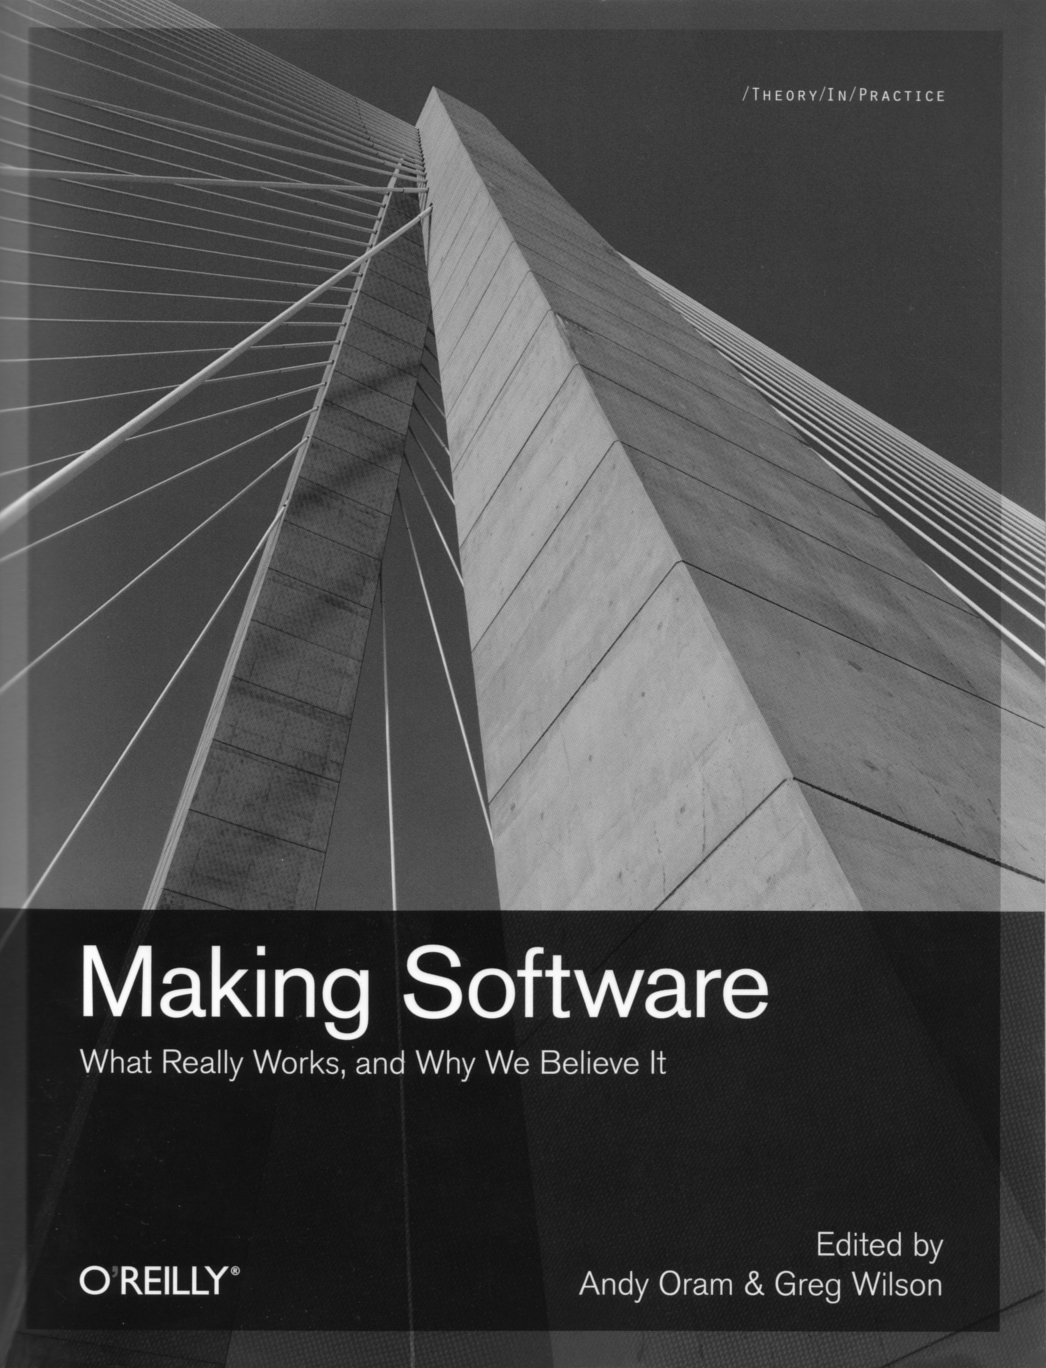
\includegraphics[width=250pt]{../images/backmatter/making.pdf}
\end{figure}

Many claims are made about how certain tools, technologies, and
practices improve software development. But which are true, and which
are merely wishful thinking? In \emph{Making Software}, leading
researchers and practitioners present chapter-length summaries of key
empirical findings in software engineering, and answer questions like:

\vspace{-0.1cm}

\begin{aosaitemize}

\item Are some programmers really ten times more productive than others?

\item Does writing tests first help you develop better code faster?

\item Can code metrics predict the number of bugs in a piece of software?

\item Does using design patterns actually make software better?

\item What effect does personality have on pair programming?

\item What matters more: how far apart people are geographically, or how far apart they are in the org chart?

\end{aosaitemize}

\vspace{-0.2cm}

\setlength{\parskip}{0.15cm}

\noindent As with \emph{The Architecture of Open Source Applications}, royalties
from \emph{Making Software} will be donated to Amnesty International.

\noindent \emph{Making Software: What Really Works, and Why We Believe It} \\
edited by Andy Oram and Greg Wilson \\
O'Reilly Media, 2010, 978-0596808327 \\
\url{http://oreilly.com/catalog/9780596808303}

\normalfont

\pagebreak
\thispagestyle{empty}


%% \begin{chapter}*{Colophon}
%% Based on EN-Revision r229
\begin{chapter}*{奥付}

%% The image on the cover is a photograph of Chris Denison's \emph{48
%% Free Street Mural} in Portland, Maine, taken by Peter Dutton.\\
表紙の画像はChris Denisonの\emph{48 Free Street Mural} in Portland, Maineからのもので、撮影者はPeter Duttonである。\\

\noindent
%% The cover font is Junction by Caroline Hadilaksono.  The text font is \TeX
%% Gyre Termes and the heading font is \TeX Gyre Heros, both by Bogus\l{}aw
%% Jackowski and Janusz M. Nowacki.  The code font is Inconsolata by Raph Levien.
表紙のフォントはCaroline HadilaksonoによるJunctionである。テキストのフォントは\TeX
Gyre Termesで見出しのフォントは\TeX Gyre Heros、どちらもBogus\l{}aw
JackowskiとJanusz M. Nowackiの作品だ。コードのフォントはRaph LevienによるInconsolataである。

\end{chapter}

% add a blank page at the end to satify Lulu's distribution requirements
\pagebreak
\thispagestyle{empty}
\mbox{}



\end{document}
